% Options for packages loaded elsewhere
\PassOptionsToPackage{unicode}{hyperref}
\PassOptionsToPackage{hyphens}{url}
%
\documentclass[
]{book}
\usepackage{amsmath,amssymb}
\usepackage{lmodern}
\usepackage{iftex}
\ifPDFTeX
  \usepackage[T1]{fontenc}
  \usepackage[utf8]{inputenc}
  \usepackage{textcomp} % provide euro and other symbols
\else % if luatex or xetex
  \usepackage{unicode-math}
  \defaultfontfeatures{Scale=MatchLowercase}
  \defaultfontfeatures[\rmfamily]{Ligatures=TeX,Scale=1}
\fi
% Use upquote if available, for straight quotes in verbatim environments
\IfFileExists{upquote.sty}{\usepackage{upquote}}{}
\IfFileExists{microtype.sty}{% use microtype if available
  \usepackage[]{microtype}
  \UseMicrotypeSet[protrusion]{basicmath} % disable protrusion for tt fonts
}{}
\makeatletter
\@ifundefined{KOMAClassName}{% if non-KOMA class
  \IfFileExists{parskip.sty}{%
    \usepackage{parskip}
  }{% else
    \setlength{\parindent}{0pt}
    \setlength{\parskip}{6pt plus 2pt minus 1pt}}
}{% if KOMA class
  \KOMAoptions{parskip=half}}
\makeatother
\usepackage{xcolor}
\usepackage{longtable,booktabs,array}
\usepackage{calc} % for calculating minipage widths
% Correct order of tables after \paragraph or \subparagraph
\usepackage{etoolbox}
\makeatletter
\patchcmd\longtable{\par}{\if@noskipsec\mbox{}\fi\par}{}{}
\makeatother
% Allow footnotes in longtable head/foot
\IfFileExists{footnotehyper.sty}{\usepackage{footnotehyper}}{\usepackage{footnote}}
\makesavenoteenv{longtable}
\usepackage{graphicx}
\makeatletter
\def\maxwidth{\ifdim\Gin@nat@width>\linewidth\linewidth\else\Gin@nat@width\fi}
\def\maxheight{\ifdim\Gin@nat@height>\textheight\textheight\else\Gin@nat@height\fi}
\makeatother
% Scale images if necessary, so that they will not overflow the page
% margins by default, and it is still possible to overwrite the defaults
% using explicit options in \includegraphics[width, height, ...]{}
\setkeys{Gin}{width=\maxwidth,height=\maxheight,keepaspectratio}
% Set default figure placement to htbp
\makeatletter
\def\fps@figure{htbp}
\makeatother
\usepackage[normalem]{ulem}
\setlength{\emergencystretch}{3em} % prevent overfull lines
\providecommand{\tightlist}{%
  \setlength{\itemsep}{0pt}\setlength{\parskip}{0pt}}
\setcounter{secnumdepth}{5}
\usepackage{booktabs}
\ifLuaTeX
  \usepackage{selnolig}  % disable illegal ligatures
\fi
\usepackage[]{natbib}
\bibliographystyle{plainnat}
\IfFileExists{bookmark.sty}{\usepackage{bookmark}}{\usepackage{hyperref}}
\IfFileExists{xurl.sty}{\usepackage{xurl}}{} % add URL line breaks if available
\urlstyle{same} % disable monospaced font for URLs
\hypersetup{
  pdftitle={Vascular Surgery Exam Prep},
  pdfauthor={Editors: Adam Johnson, MD, MPH; Matt Smith, MD, PhD; and Audible Bleeding},
  hidelinks,
  pdfcreator={LaTeX via pandoc}}

\title{Vascular Surgery Exam Prep}
\author{Editors: Adam Johnson, MD, MPH; Matt Smith, MD, PhD; and Audible Bleeding}
\date{DRAFT - 2022-08-09}

\begin{document}
\maketitle

{
\setcounter{tocdepth}{1}
\tableofcontents
}
\hypertarget{about}{%
\chapter{About}\label{about}}

This content was developed by the \href{https://www.audiblebleeding.com/about-1/}{Audible Bleeding Team} to accompany our board review podcast series.
Each chapter covers a key domain of vascular surgery, essential for board review preparation, and is associated with an Audible Bleeding episode which you can access through the link embeded into the text.

\hypertarget{usage}{%
\section{Usage}\label{usage}}

This e-book is not intended to be a comprehensive board review guide, but instead serves as an easily accessible resource, paired with our podcast content to help streamline exam preparation.

\hypertarget{comments-questions-or-contributions}{%
\section{Comments, Questions or Contributions}\label{comments-questions-or-contributions}}

Please visit our \href{https://github.com/adam-mdmph/VS-Board-Review}{github page} or \href{mailto:audiblebleeding@vascularsociety.org}{send us an email}.

\hypertarget{cerebrovascular}{%
\chapter{Cerebrovascular}\label{cerebrovascular}}

\textbf{07 Jan 2019:} \emph{Adam Johnson, MD, MPH; Nicole Rich, MD, MPH; Kevin
Kniery, MD, MPH}

\hypertarget{available-guidelines}{%
\section{Available Guidelines}\label{available-guidelines}}

\href{https://www.jvascsurg.org/article/S0741-5214(21)00893-4/fulltext}{Society for Vascular Surgery clinical practice guidelines for
management of extracranial cerebrovascular
disease}
\citep{aburahmaSocietyVascularSurgery2022}

\hypertarget{presentation-and-diagnosis}{%
\section{Presentation and Diagnosis}\label{presentation-and-diagnosis}}

\begin{enumerate}
\def\labelenumi{\arabic{enumi}.}
\item
  \textbf{What is the definition of crescendo TIAs?}

  Frequent repetitive neurological attacks without complete resolution
  of the deficit between the episodes, usually over a 24 hour period.
  The result of which is the same neurological deficit. If the patient
  exhibits progressive deterioration in neurological function between
  TIA episodes this is classified as a stroke in evolution not a
  crescendo TIA.
\item
  \textbf{Who needs to be screened for carotid disease?}

  Not everyone should be screened for carotid disease, however, as
  only 15\% of patients who have a stroke experience a warning TIA
  prior to their event, there is merit in screening high risk
  patients. The purpose of carotid bifurcation imaging is to detect
  ``stroke-prone'' carotid bifurcation plaque and identify a high-risk
  patient likely to benefit from therapy designed to reduce stroke
  risk.

  Traditionally, the clinical sign associated with carotid stenosis is
  the prescence of a neck bruit on auscultation. Focal ipsilateral
  carotid bruits in symptomatic patients has a sensitivity of 63\% and
  a specificity of 61\% for high-grade carotid stenosis (range,
  70\%-99\%). As these figures suggest the absence of carotid bruit does
  not absolutely exclude the presence of a significant carotid
  bifurcation lesion, therefore additional criteria are used to
  determine which patients would benefit from screening:

  \begin{itemize}
  \item
    Evidence of clinically significant peripheral vascular disease
    regardless of age
  \item
    Patients aged \textgreater65 years with a history of one or more of the
    following atherosclerotic risk factors:

    \begin{itemize}
    \item
      CAD
    \item
      Smoking
    \item
      Hypercholesterolemia
    \end{itemize}
  \item
    In general, the more risk factors present, the higher the yield
    of screening for the patient.
  \item
    The benefit of prophylactic treatment of high grade stenosis is
    estimated at a 1-2\% stroke reduction risk per year.
    \citep{naylorWhyManagementAsymptomatic2015}
  \item
    Keep in mind that intervention (CEA/CAS) has only demonstrated a
    benefit in asymptomatic patient with life expectancy greater
    than 3 years. \citep{bulbuliaAsymptomaticCarotidSurgery2017, halliday10yearStrokePrevention2010, rosenfieldRandomizedTrialStent2016}
  \end{itemize}
\item
  \textbf{Ultrasound Imaging}

  \begin{itemize}
  \item
    US is considered the best, least invasive, and cost effective
    method for detecting carotid stenosis on screening.
  \item
    50-69\% stenosis of ICA - US has a low sensitivity for 50-69\%
    stenosis. A negative ultrasound in symptomatic patients
    necessitates additional imaging. Typically on scanning if 50-69\%
    ICA stenosis is present:

    \begin{itemize}
    \tightlist
    \item
      PSV 125-229 cm/sec
    \item
      EDV 40-100
    \item
      Internal/Common Carotid PSV Ratio 2-4
    \end{itemize}
  \item
    70-99\% stenosis of ICA- Typically on scanning:

    \begin{itemize}
    \item
      PSV \textgreater/= 230 cm/sec
    \item
      EDV \textgreater100 (EDV \textgreater{} 140 cm/sec most sensitive for stenosis \textgreater80\%)
    \item
      Internal/Common Carotid PSV Ratio \textgreater{} 4
    \end{itemize}
  \item
    Velocity-based estimation of carotid artery stenosis may need to
    be adjusted in certain circumstances:

    \begin{itemize}
    \item
      Higher velocities in women than in men.
    \item
      Higher velocities in the presence of contralateral carotid
      artery occlusion.
    \end{itemize}
  \item
    High carotid bifurcation, severe arterial tortuosity, extensive
    vascular calcification, and obesity may also reduce the accuracy
    of US imaging.
  \end{itemize}
\item
  \textbf{Other Imaging Modalities}

  \begin{itemize}
  \item
    CTA

    \begin{itemize}
    \item
      Pro - fast, sub-millimeter spatial resolution, visualize
      surrounding structures.
    \item
      Con - cost, contrast exposure.
    \end{itemize}
  \item
    MRA

    \begin{itemize}
    \item
      Pro - no contrast administered; can analyze plaque
      morphology.
    \item
      Con - Does not visualize calcium in plaque; overestimates
      the degree of stenosis (False positive for 50-69\% to be read
      as \textgreater70\%).
    \end{itemize}
  \item
    Catheter-based digital subtraction imaging (DSA)

    \begin{itemize}
    \item
      Still considered by many the gold-standard imaging modality.
    \item
      Reserved for individuals with conflicting less-invasive
      imaging or those considered for CAS.
    \item
      Con - cost, contrast, and risk of stroke.
    \end{itemize}
  \end{itemize}
\end{enumerate}

\hypertarget{management}{%
\section{Management}\label{management}}

\hypertarget{optimal-medical-therapy}{%
\subsection{Optimal medical therapy}\label{optimal-medical-therapy}}

First line management for asymptomatic patients with carotid stenosis is
medical optimisation of risk factors.

\textbf{Hypertension}

\begin{itemize}
\item
  Blood pressure reduction, with a target of \textless140/90 mmHg through
  lifestyle interventions and anti-hypertensive treatment is
  recommended in individuals who have hypertension with asymptomatic
  carotid atherosclerosis or those with TIA or stroke after the
  hyper-acute period.
\item
  Each 10-mm Hg reduction in blood pressure among hypertensive
  patients decreases the risk of stroke by 33\%.
\end{itemize}

\textbf{Diabetes}

\begin{itemize}
\tightlist
\item
  In diabetic patients glycaemic control to nearly normoglycemic
  levels (target hemoglobin A1C \textless7\%) is recommended to reduce
  microvascular complications and, with a smaller evidence base,
  macrovascular complications other than stroke.
\end{itemize}

\textbf{Hypercholesterolaemia}

\begin{itemize}
\item
  Risk of stroke decreased by \textgreater15\% for every 10\% reduction in serum
  LDL in patients with known coronary or other atherosclerosis.
\item
  Statin agents are recommended targetting LDL of 100 mg/dL, for those
  with coronary heart disease or symptomatic atherosclerotic disease,
  and LDL of 70 mg/dL for very high-risk persons with multiple risk
  factors.
\item
  High dose statin therapy in patients with TIA/stroke reduce future
  rates of stroke or cardiovascular events but not overall mortality
  at 5 years. \citep{karamHighDoseAtorvastatinStroke2008}
\end{itemize}

\textbf{Smoking Cessation} - Encouraging smoking cessation is paramount for
these patients. Physician counseling is an important and effective
intervention that reduces smoking in patients by 10\% to 20\%. (REF)

\textbf{Antithrombotic therapy} - Aspirin is the only antiplatelet agent that
has demonstrated improved benefit in asymptomatic patients with carotid
atherosclerosis.

\hypertarget{carotid-endarterectomy}{%
\subsection{Carotid endarterectomy}\label{carotid-endarterectomy}}

\textbf{Indications for Surgical Intervention}

\begin{itemize}
\item
  Recommendations on when to operate after a TIA/stroke.

  \begin{itemize}
  \item
    Acute stroke with a fixed neurologic deficit of \textgreater6h duration -
    When the patient is medically stable, intervention in 14 days or
    less after stroke is preferable.
    \citep{rothwellEndarterectomySymptomaticCarotid2004, meershoekTimingCarotidIntervention2018}
  \item
    Consider urgent intervention in a medically stable patient with
    mild-moderate neurologic deficit, if there is a significant area
    of ischemic penumbra at risk for progression on imaging that is
    contributing to the patient's presentation.
  \item
    Stroke in evolution (fluctuating / evolving neurological
    deficit) or crescendo TIA (repetitive transient ischemia with
    improvement between events) - If the patient's neurological
    status is not stabilized by medical intervention then an urgent
    CEA should be considered.
  \item
    In this clinical context CEA is preferred to CAS based on an
    increased embolic potential of carotid lesions.
    \citep{rantnerEarlyEndarterectomyCarries2017}
  \item
    Management of acute stroke \citep{powers2018GuidelinesEarly2018}

    \begin{itemize}
    \item
      \textless4.5hrs from onset of symptoms - medical thrombolysis with
      tPA unless contraindicated.

      \begin{itemize}
      \item
        Patient age \textgreater80 and diabetes are contraindications to
        tPA administration after 3hrs.
      \item
        Other contraindications include - hypertension,
        intracranial hemorrhage, recent stroke or cranial
        trauma, spine/brain surgery within 3 months, GI bleed
        within 21 days.
      \end{itemize}
    \item
      \textless6hr from onset of symptoms - catheter directed therapy
    \end{itemize}
  \end{itemize}
\item
  What is the only emergent indication for CEA?

  \begin{itemize}
  \tightlist
  \item
    Crescendo TIAs or a stroke in evolution with a surgically
    correctable lesion identified on imaging.
  \end{itemize}
\end{itemize}

\textbf{CEA Intraoperative Techniques}

\begin{itemize}
\item
  General concepts

  \begin{itemize}
  \tightlist
  \item
    Patch angioplasty or eversion endarterectomy are recommended
    over primary arterial closure to reduce early and late
    complications of CEA (GRADE 1, Level of Evidence A). \# Add
    Reference
  \end{itemize}
\item
  Neuromonitoring/Shunting options during a carotid endarterectomy

  \begin{itemize}
  \item
    Procedure performed under local/regional anesthesia with direct
    neurological monitoring - the benefit being that the patient is
    awake and moving to command throughout the case. Improved
    neuromonitoring, however, has not been shown to reduce MI
    (myocardial infarction?) rate with CEA.
  \item
    Determining shunt use using stump pressure- Clamp the inflow and
    place a butterfly attached to a-line tubing into the internal
    carotid atery. If the stump pressure is \textgreater{} 40 mmHg the surgeon
    can chose to proceed without shunt placement, if \textless{} 40mmHg then
    a shunt should be placed prior to proceeding.
  \item
    EEG Neuromonitoring - EEG tech places neuromonitoring, monitored
    by the technician and neurologist remotely intraoperatively.
    Generally the surgeon should clamp the ICA for 3 minutes before
    proceeding, if the patient develops neurological deficit/EEG
    abnormalities then unclamp, await normalization of EEG, then
    proceed.
  \item
    Non-selective shunting - the surgeon uses a shunt for all CEAs
    as standard practice, this is often done for all CEAs performed
    under general anaesthesia.
  \end{itemize}
\item
  Techniques to reach high internal carotid lesions?

  \begin{itemize}
  \item
    A good knowledge of the available imaging while preparing for
    the procedure is essential when considering the level of the
    carotid bifurcation.
  \item
    Nasotracheal intubation will allow for jaw closure and neck
    extension to facilitate exposure of higher lesions.
  \item
    Division of the posterior belly of the digastric muscle can be
    performed to improve exposure of a high bifurcation. Care should
    be taken to identify and preserve the glossopharyngeal nerve.
  \item
    Styloidectomy.
  \item
    ENT surgeon assisted mandible subluxation with assistance if
    previous techniques fail.
  \end{itemize}
\item
  What is the best technique for a patient with an anatomically kinked
  internal carotid artery?

  \begin{itemize}
  \item
    Eversion carotid endarterectomy (only indication for selection
    for this technique over patch endarterectomy), transection
    allows for reduction of redundancy at re-anastamosis.
  \item
    Otherwise, no advantage has been shown between eversion or
    patch, both can be shunted.
  \end{itemize}
\item
  Nerve Injuries -- where you would encounter these and, if injured,
  what deficit would be seen?

  \begin{itemize}
  \item
    Hypoglossal: Most commonly injured. Usually passes above the
    bifurcation of the carotid artery. If injured the tongue will
    deviate toward the side of injury on protrusion.
  \item
    Glossopharyngeal: Commonly injured during high dissections.
    Found under the posterior digastric muscle. Injury can be
    devastating for patients resulting in difficulty swallowing and
    high aspiration risk.
  \item
    Vagus: Usually found adjacent and lateral to the common carotid.
    Injury can occur with carotid clamping. Patients develop
    hoarseness due to innervation of the laryngeal muscles from the
    recurrent laryngeal nerve which is a branch of the vagus.
  \item
    Marginal Mandibular: Branch of the facial nerve. Runs inferiorly
    to the angle of the mandible. Commonly a retraction injury
    during high dissections leading to the corner of the ipsilateral
    lip drooping, can be confused with a significant neurological
    deficit following the case.
  \end{itemize}
\end{itemize}

\textbf{Postoperative Complications}

\begin{itemize}
\item
  What to do if the patient develops neuro deficits following carotid
  endarterectomy: Two main concerns- an intimal flap causing
  thrombosis or an embolic event resulting in a stroke. Perform a
  thorough neurological exam to confirm in operated corotid territory.

  \begin{itemize}
  \item
    If in OR -- perform duplex, if normal open wound and perform a
    cerebral angiogram.
  \item
    If in Recovery or on the floor -- many would consider CTA first
    line vs duplex to look for thrombosis.
  \end{itemize}
\item
  Risk factors and how to manage hyperperfusion syndrome?

  \begin{itemize}
  \item
    Defined as an ipsilateral headache, hypertension, seizures, and
    focal neurological deficits likely in distribution of the
    carotid. Can present 2-3 days post surgery.
  \item
    Patients with uncontrolled hypertension are at risk for
    hyperperfusion syndrome, clinical practice guidelines from SVS
    recommend strict BP control following CEA, with target pressure
    being less than 140/80mmHg.
  \end{itemize}
\item
  High risk groups

  \begin{itemize}
  \tightlist
  \item
    ESRD patients have higher rates of perioperative stroke, but
    also have higher rates of stroke if not revascularized.
    \citep{klarinPerioperativeLongtermImpact2016}
  \end{itemize}
\end{itemize}

\textbf{Long term complications and follow up}

\begin{itemize}
\item
  Recommend f/u US duplex of bilateral carotids at \textless/=30 days. \textgreater/=
  50\% stenosis further imaging is indicated.
\item
  Contralateral stenosis:

  \begin{itemize}
  \item
    The risk of progression for moderate stenosis at the initial
    surveillance to severe stenosis in the contralateral artery can
    be as high as 5 times.
  \item
    Requires post-operative surveillance.
  \end{itemize}
\end{itemize}

\hypertarget{carotid-artery-stenting}{%
\subsection{Carotid Artery Stenting}\label{carotid-artery-stenting}}

\begin{itemize}
\item
  In patients aged \textgreater70 the risk of intra- or post procedure stroke was
  the highest, if undergoing CAS, presumably due to calcified disease
  in the arch.

  \begin{itemize}
  \item
    Lesion-specific characteristics are thought to increase the risk
    of cerebral vascular events after CAS and include a ``soft''
    lipid-rich plaque identified on noninvasive imaging, extensive
    (15 mm or more) disease, a pre-occlusive lesion, and
    circumferential heavy calcification.
  \item
    This risk can be reduced, but not eliminated, by using
    flow-reversal embolic protection rather than distal filter
    protection.
  \end{itemize}
\item
  Limited data is available on CAS in asymptomatic patients -
  currently is not supported by guidelines or considered reimbursable.
\item
  Consider CAS in symptomatic patients with \textgreater50\% stenosis who are poor
  candidates for CEA due to severe uncorrectable medical comorbidities
  and/or anatomic considerations:

  \begin{itemize}
  \item
    Ipsilateral neck dissection or XRT - equivalent periprocedural
    stroke rate to CEA, but increased later stroke rate. CEA higher
    rates of cranial nerve damage (9\%).
    \citep{giannopoulosRevascularizationRadiationinducedCarotid2018}
  \item
    Contralateral vocal cord paralysis.
  \item
    Lesions that extend proximally to the clavicle or distal to C2.
  \end{itemize}
\item
  Transfemoral Approach vs Transcarotid approach

  \begin{itemize}
  \tightlist
  \item
    ROADSTER Trial - single arm study with flow reversal for
    cerebral protection. Suggested lower rates of post-op stroke in
    patients undergoing TCAR.
  \end{itemize}
\item
  Post-CAS follow up - Dual-platelet therapy should be continued for 1
  month after the procedure, and aspirin should be continued
  indefinitely.

  \begin{itemize}
  \tightlist
  \item
    In stent restenosis (\textgreater50\%) - repeat angioplasty or stent have
    low incidence of periprocedural stroke but failed to improve
    long term stroke/death/MI or patency rates.
    \citep{chungPercutaneousInterventionCarotid2016a}
  \end{itemize}
\end{itemize}

\hypertarget{management-of-uncommon-disease-presentations}{%
\subsection{Management of Uncommon Disease Presentations}\label{management-of-uncommon-disease-presentations}}

\begin{itemize}
\item
  Occluded Carotid: What is the management of an occluded carotid?

  \begin{itemize}
  \tightlist
  \item
    Leave it alone.
  \end{itemize}
\item
  What if an occluded carotid on imaging is still causing TIAs?

  \begin{itemize}
  \item
    External carotid endarterectomy and ligation of the internal
    carotid.
  \item
    The addition of oral anticoagulation is likely to reduce the
    rate of recurrent stroke.
  \end{itemize}
\item
  What if the patient has severe vertebrobasilar insufficiency and
  carotid artery disease?

  \begin{itemize}
  \tightlist
  \item
    Should undergo carotid revascularization first to improve flow.
    Then reassess for vertebrobasilar insufficency.
  \item
    Vertebrobasilar insufficiency characterized by dizziness,
    ataxia, nausea, vertigo and bilateral weakness.
    \citep{limanetoPathophysiologyDiagnosisVertebrobasilar2017}
  \end{itemize}
\item
  What about tandem lesions in the carotid in a symptomatic patient,
  carotid bulb and carotid siphon lesion (high ICA)? How should you
  treat this?

  \begin{itemize}
  \tightlist
  \item
    Treat carotid bulb first, likely to be the embolic source.
  \end{itemize}
\item
  Carotid artery dissection

  \begin{itemize}
  \item
    Patients with carotid dissection should be initially treated
    with antithrombotic therapy (antiplatelet agents or
    anticoagulation) (GRADE 1, Level of Evidence C).
  \item
    Indications for endovascular treatment of carotid artery
    dissection \citep{cohenSinglecenterExperienceEndovascular2012, markusAntiplateletTherapyVs2019a, phamEndovascularStentingExtracranial2011}

    \begin{itemize}
    \item
      Ongoing symptoms on best medical therapy
    \item
      Contraindication to antithrombotics
    \item
      Pseudoaneurysm
    \end{itemize}
  \end{itemize}
\item
  Simultaneous coronary and carotid disease

  \begin{itemize}
  \item
    Patients with symptomatic carotid stenosis will benefit from CEA
    before or concomitant with CABG. The timing of the intervention
    depends on the clinical presentation and institutional
    experience (GRADE 1, Level of Evidence B).
  \item
    Patients with severe bilateral asymptomatic carotid stenosis,
    including stenosis and contralateral occlusion, should be
    considered for CEA before or concomitant with CABG (GRADE 2,
    Level of Evidence B).
  \item
    Patients undergoing simultaneous CEA/CABG demonstrate highest
    mortality. \citep{naylorSystematicReviewOutcomes2003}
  \end{itemize}
\end{itemize}

\hypertarget{prospective-trials---must-reads}{%
\section{Prospective Trials - MUST READS}\label{prospective-trials---must-reads}}

\begin{enumerate}
\def\labelenumi{\arabic{enumi}.}
\item
  Asymptomatic Carotid Atherosclerosis Study (ACAS)

  \begin{itemize}
  \item
    Compared medical management with CEA in asymptomatic patients
    with \textgreater{} 60\% stenosis.
  \item
    5-year stroke and death rate was 5.1\% vs 11\%.
  \item
    In women, the benefit of CEA was not as certain as 5y stroke and
    death rates were 7.3\% vs.~8.7\%.
  \item
    This trial was conducted pre-statin and clopidogrel era.
  \end{itemize}
\item
  North American Symptomatic Carotid Endarterectomy Trial (NASCET)
  \citep{northamericansymptomaticcarotidendarterectomytrialcollaboratorsBeneficialEffectCarotid1991}

  \begin{itemize}
  \item
    Compared medical management vs CEA for symptomatic patients with
    moderate (50-69\%) and severe stenosis (\textgreater70\%)
  \item
    Only moderate impact for patients with moderate stenosis
    (50-69\%)
  \item
    Symptomatic patients with \textgreater70 \% stenosis benefited from CEA, at
    18 months 7\% major stroke in surgical arm, and a 24\% stroke rate
    in medical arm. 29\% reduction in 5-year risk of stroke or death.

    \begin{itemize}
    \tightlist
    \item
      Patients with severe \textgreater70\% stenosis had such a dramatic
      effect the trial was stopped early for this subset and all
      referred for endarterectomy.
    \end{itemize}
  \item
    No benefit is shown in symptomatic patients with \textless{} 50\% stenosis
  \item
    European studies have shown similar results

    \begin{itemize}
    \item
      ACST = ACAS
    \item
      ECST = NASCET.
    \end{itemize}
  \item
    \textbf{Take a listen!} \href{https://www.audiblebleeding.com/2021/09/29/landmark-papers-nascet/}{Click hear to listen to Dr.~William Jordan
    discuss this landmark
    paper!}
  \end{itemize}
\item
  Carotid Revascularization Endarterectomy versus Stenting Trial
  (CREST).

  \begin{itemize}
  \item
    Compared CEA vs.~CAS in both symptomatic and asymptomatic
    patients.
  \item
    Composite endpoint of 30-day stroke, MI, death equivalent
    between CEA and CAS.
  \item
    CAS had a significantly higher incidence of stroke and death
    than CEA and CEA higher incidence of MI.

    \begin{itemize}
    \tightlist
    \item
      Follow up at 10 years demonstrated no difference in
      composite stroke/MI/death but increased rate of stroke/death
      in stented patients likely attributable to increased
      periprocedural stroke. \citep{brottLongTermResultsStenting2016b}
    \end{itemize}
  \item
    Subanalyses identified that older patients (\textgreater70y) had better
    outcomes after CEA than CAS, the QOL impact of stroke was more
    significant than that of MI, and anatomic characteristics of
    carotid lesions (longer, sequential, remote) were predictive of
    increased stroke and death after CAS.
  \item
    Unfortunately, this study provides a benchmark to strive for,
    but no other large trials have achieved these results.
  \end{itemize}
\item
  ROADSTER

  \begin{itemize}
  \item
    Single arm feasibility trial of transcarotid carotid stenting.
  \item
    The results of the ROADSTER trial demonstrate that the use of
    the ENROUTE Transcarotid NPS is safe and effective at preventing
    stroke during CAS. The overall stroke rate of 1.4\% is the lowest
    reported to date for any prospective, multicenter clinical trial
    of CAS.
  \end{itemize}
\item
  Trials to look out for in the next few years:

  \begin{itemize}
  \item
    CREST-2 - a multicenter, randomized controlled trial underway
    evaluating revascularization against modern intensive medical
    management.
  \item
    ACT-1 and ACST-2- the role of intervention in asymptomatic
    patients, designed to compare the early and long-term results of
    CEA vs CAS and best medical management.
  \item
    ROADSTER-2 - TCAR.
  \end{itemize}
\end{enumerate}

\hypertarget{upper-extremity-and-thoracic-outlet}{%
\chapter{Upper Extremity and Thoracic Outlet}\label{upper-extremity-and-thoracic-outlet}}

\textbf{21 Jan 2021}: \emph{Kush Sharma, MD and Ashraf Mansour, MD}

\hypertarget{anatomy-exposure-of-vessels}{%
\section{Anatomy/ Exposure of Vessels}\label{anatomy-exposure-of-vessels}}

\textbf{What are the zones of the upper extremity?}
\citep{illig57UpperExtremity2019, illig57UpperExtremity2019}

Division of the upper extremity into three zones:

\textbf{1. Intrathoracic Zone:} Inclusive of the aortic arch and its
branches, innominate artery (dividing into right subclavian and right
common carotid), left subclavian artery and left common carotid artery,
as well as the innominate veins, and SVC.

\textbf{2. Thoracic Outlet:} Extends from the base of neck to the axila.
Includes the subclavian, proximal vertebral, and proximal axillary
arteries, as well as the corresponding veins).

\textbf{3. Axilla to Fingers:} The arm.

\textbf{What are some common exposures for major upper extremity arteries?}

\textbf{Right Subclavian Artery:} For proximal artery exposure a medial
sternotomy is required, for the mid-distal artery a right
supraclavicular approach is needed.

\textbf{Left Subclavian Artery:} An anterolateral thoracotomy is required in
emergent settings for proximal left subclavian artery control. For
proximal, mid and distal exposure is required a ``trap door'' exposure is
used: anterolateral thoracotomy, third space sternotomy, and left
supraclavicular incision.

\textbf{Supraclavicular Incision:} After division of the platysma and
clavicular head of the SCM, a fat pat of varying thickness is
encourntered which contains the omohyoid muscle. This should be divided
and placed supero-laterally. At this point, the anterior scalene muscle
is exposed medially with the phrenic nerve running in a lateral to
medial direction, which should be identfied and preseved. In a
carotid/subclavian bypass division of the anterior scalene should be
performed as close to the first rib as possible. Once divided the
subclavian artery is exposed.

\textbf{Axillary Artery:} Exposure is gained through an infraclavicular
inicision, below the middle third of the clavicle. Pectoralis major is
divided and pectoralis minor is freed at the lateral margin of the
wound. The axillary vein should be identified and followed supero-deeply
to identify and expose the artery.

Anatomically bound by the first rib proximally and the lateral edge of
the teres major muscle distally. For exposure of the first part of the
axillary artery, the ipsilateral arm is abducted approximately 90
degrees and a horizontal skin incision 2 cm below the middle third of
the clavicle should be made. The underlying pectoralis major is split by
bluntly separating the fibers, exposing the tough clavipectoral fascia.
At the lateral wound margin, the pectoralis minor can be freed and
laterally retracted. The axillary vein is the first structure to be
encountered in the fascia and the artery lies just superior and deep to
the vein. Make sure to protect the nerves of the brachial plexus which
lie deep to the first part of axillary artery and are at risk of injury
during blind placement of occluding arterial clamps.
\citep{garygwindAnatomicExposuresVascular2013}

\textbf{What steps are involved for brachial, radial and ulnar artery
exposure?}

\textbf{Brachial Artery, Upper Arm:} The brachial artery's superficial
location makes it vulnerable to injury and accounts for most vascular
injuries of the upper extremities. Brachial artery exposure involves a
5-8 cm longitudinal incision in the groove between the biceps/triceps
muscles on the medial aspect of the arm. In the lower half of the arm,
take care to avoid basilic vein damage as it runs in the subcutaneous
tissue. The neurovascular bundle is exposed by incising the deep fascia
at the medial border of the biceps muscle, which then should be
retracted anteriorly. The basilic vein should be indetified and
retracted into the posterior wound. On opening the brachial sheath the
median nerve is the most superficial structure and should be identified,
protected and retracted. The brachial artery lies deep to the median
nerve and is flanked by two brachial veins. Be midful that the ulnar
nerve lies posteriorly.

\textbf{Brachial Artery, Antecubital Fossa:} Exposure of the brachial artery
in the antecubital fossa requires a transverse skin incision 1 cm distal
to the midpoint of the antecubital crease. After deepening, mobilize the
basilic vein medially to avoid injury. The medial antebrachial cutaneous
nerve should be identified and protected. The bicipital aponeurosis
should be divided to exposure the brachial artery, which is flanked by
two deep veins crossing tributaries. To isolate the brachial artery
ligation and division of these tributaries is required.

The brachial artery bifurcates at the radial tuberosity into its radial
and ulnar branches. Immediately after the ulnar artery arises from the
bifurcation origin, it gives off a short common interosseous branch,
which bifurcates at the hiatus in the proximal interosseous membrane.

\textbf{Radial Artery at the Wrist:} This requires a 2-3 cm longitudinal
incision generally between the palpable radial artery and cephalic vein.
Incision of the antebrachial fascia medially to the radius should expose
the radial artery. Two veins accompany the artery and should be
dissected away to isolate the artery. The superficial radial nerve and
its medial/lateral branches course between the cephalic vein and radial
artery in this area.

\textbf{Ulnar Artery:} The ulnar artery courses beneath the superficial
flexor muscles of the proximal forearm, emerging near the ulnar border
at the midpoint between the elbow and the wrist. In the distal forearm,
the ulnar artery runs just deep to the antebrachial fascia and is easily
exposed through a longitudinal incision placed radially to the flexor
carpi ulnaris. The palmar branch of the ulnar nerve courses
superficially to the antebrachial fascia and should be preserved during
arterial exposure to avoid injury.

\textbf{What common aberrant upper extremity/arch anatomy is important to be
aware of?}

\begin{itemize}
\item
  \textbf{Bovine Arch:} Where the inominate and left common carotid
  arteries share a common origin.
\item
  \textbf{Abberant Vertebral Artery:} Where the vertebral artery arises
  directly from the aortic arch.
\item
  \textbf{Aberrant Right Subclavian Artery:} Where there is no innominate
  artery and instead the right common carotid arises directly from the
  aorta. Confusingly the right subclavian artery, then orginates from
  the aortic arch distal to the left subclavian artery. To supply the
  right arm it therefore, needs to pass behind the eosophagus.
  (Dysphagia Lusoria)
\end{itemize}

\hypertarget{epidemiology-etiology-and-diagnostic-evaluation}{%
\section{Epidemiology, Etiology, and Diagnostic Evaluation}\label{epidemiology-etiology-and-diagnostic-evaluation}}

\textbf{How does evaluation of upper extremity ischemia differentiate from
lower extremity ischemia?} \citep{shuja117UpperExtremity}

\begin{itemize}
\item
  Upper extremity ischemia \textless5\% of patients with limb ischemia and in
  contrast to lower extremity, atherosclerosis is not a major
  contributor to upper extremity ischemia
\item
  Vast majority of cases caused by autoimmune/connective tissue
  disorders
\end{itemize}

\textbf{How can upper extremity disease be classified?}

Anatomic Location:

\begin{itemize}
\tightlist
\item
  Large vs.~Small Vessel
\end{itemize}

Disease Process:

\begin{itemize}
\tightlist
\item
  Vasospastic or occlusive. Vasospastic disease is more responsive to
  pharmacologic management while occlusive requiring
  endovascular/surgical management.
\end{itemize}

\textbf{How should patients be evaluated who have concern for upper extremity
disease?}

Diagnostic Evaluation

\begin{enumerate}
\def\labelenumi{\arabic{enumi}.}
\item
  Detailed H+P evaluation (pulse palpation, auscultation at
  supraclavicular/infraclavicular fossa may reaveal a bruit concerning
  for subclavian artery stenosis, upper extremity neurovascular/skin
  exam)
\item
  Brachial/forearm blood pressures and if suspected claudication,
  measured at rest and 2-5 minutes after exercise. Look for a gradient
  of \textgreater20 mmHg is considered significant
\item
  Some or all of 6 P's of acute limb ischemia with symptoms occurring
  within 14 days are deemed acute
\item
  Doppler insonation of radial, ulnar, palmar, and digital arteries
\item
  Vascular Lab Evaluation

  \begin{enumerate}
  \def\labelenumii{\arabic{enumii}.}
  \item
    Segmental Pressure Measurements
  \item
    Duplex Ultrasound (look for large vessel occlusive disease)
  \end{enumerate}
\item
  Other Imaging

  \begin{enumerate}
  \def\labelenumii{\arabic{enumii}.}
  \tightlist
  \item
    CTA/MRA
  \end{enumerate}
\item
  Clinical Lab tests

  \begin{enumerate}
  \def\labelenumii{\arabic{enumii}.}
  \item
    Inflammatory disorders-CBC, ESR, ANA, RF
  \item
    Hypercoagulable screening
  \end{enumerate}
\end{enumerate}

\hypertarget{operationsprocedures}{%
\section{Operations/Procedures}\label{operationsprocedures}}

\textbf{What are some indications for carotid-subclavian bypass?}

\begin{enumerate}
\def\labelenumi{\arabic{enumi}.}
\item
  Atherosclerosis
\item
  Staged revascularization prior to TEVAR for aneurysmal disease
  requiring coverage of the LSA
\end{enumerate}

\textbf{How does the exposure differentiate in transposition vs bypass?}

Exposure (Transposition vs Bypass)

\begin{itemize}
\item
  Arterial transposition via a short, transverse cervical incision
  above the clavicle between two heads of SCM (bypass is lateral to
  entire SCM)
\item
  Sub-platysmal flaps created and avoid EJ vein damage
\item
  Omohypoid divided between heads of SCM and IJ mobilized laterally
  (bypass IJ is mobilized medially to expose CCA and care must be
  taken to avoid phrenic nerve in more lateral approach)
\item
  CCA is reflected medially with vagus nerve~
\item
  On the left side, the thoracic duct is identifiable and divided
  followed by dividing the vertebral vein
\item
  Subclavian artery and proximal branches identified (anterior scalene
  is in lateral dissection)
\end{itemize}

\textbf{What are some common complications after carotid subclavian bypass in
order of highest to lowest incidence?}

Complications \citep{voigtOutcomesCarotidsubclavianBypass2019}

\begin{enumerate}
\def\labelenumi{\arabic{enumi}.}
\item
  Phrenic nerve palsy (most common) - most often managed
  conservatively.
\item
  Recurrent laryngeal palsy
\item
  Lymphatic leak
\item
  Neck hematoma
\end{enumerate}

\textbf{When carotid-subclavian bypass compared to transposition?}

\begin{enumerate}
\def\labelenumi{\arabic{enumi}.}
\item
  Vertebral artery takes origin from the subclavian artery in a very
  proximal position or is dominant over the contralateral side, then
  bypass preferred. \citep{moraschTechniqueSubclavianCarotid2009d}
\item
  For coronary-subclavian steal with patent internal mammary artery to
  coronary artery bypass graft, then Bypass (a carotid-subclavian
  transposition requires a more proximal clamp with occlusion of
  inline antegrade flow to the coronary bypass during the procedure)
  \citep{cuaReviewCoronarySubclavian2017}
\end{enumerate}

\hypertarget{vaso-occlusive-disease}{%
\section{Vaso-occlusive disease}\label{vaso-occlusive-disease}}

\textbf{What are causes and symptoms associated with subclavian/axillary
occlusive disease?} \citep{jacklcronenwettVascularDecisionMaking2020}

\begin{itemize}
\item
  Etiology: Atherosclerosis is the most common cause of
  subclavian/axillary occlusive disease. Left SCA \textgreater{} Right involvement.
  Less common causes include Takayasu disease, giant cell arteritis,
  or arterial TOS
\item
  Symptoms: Upper extremity arm/hand ischemia or neurologic symptoms
  due to subclavian-vertebral steal. Because significant collaterals,
  minimal pain on exertion even with subclavian occlusion
\end{itemize}

\textbf{What are causes and symptoms associated with brachial/forearm
occlusive disease?}

\begin{itemize}
\item
  Etiology: MCC of brachial artery occlusion is cardiac origin
  embolus. Atherosclerosis RARELY affects the brachial artery. Distal
  axillary/proximal brachial stenosis can be from repetitive trauma
  from crutch use.~
\item
  Forearm occlusive disease can be seen in advanced ESRD/DM where
  calcific atherosclerosis of radial/ulnar arteries is present. Less
  common causes include Beurger disease or Raynaud Phenomenon
\end{itemize}

\textbf{How/when is upper extremity occlusive disease treated?}

\begin{itemize}
\item
  SCA Occlusive Disease

  \begin{itemize}
  \item
    Endovascular with balloon expandable stent via femoral or
    ipsilateral brachial artery.
    \citep{chatterjeeAngioplastyAloneAngioplasty2013, bradaricEndovascularTherapyStenoOcclusive2015, sahaSubclavianArteryDisease2017} Preferred in:

    \begin{itemize}
    \item
      Short segment or ostial disease with adequate distance to
      the vertebral artery origin.
    \item
      History of neck surgery or radiation.
    \end{itemize}
  \item
    Surgery:

    \begin{itemize}
    \item
      Bypass from aortic arch through median sternotomy~
    \item
      Ipsilateral CCA to subclavian artery (bypass or
      transposition)~
    \item
      Contralateral CCA (anterior or retropharyngeal)
    \end{itemize}
  \end{itemize}
\item
  Brachial/forearm Occlusive disease~

  \begin{itemize}
  \item
    Endovascular: PTA evidence is anecdotal with stents for lesions
    unresponsive to PTA or dissection following angioplasty~
  \item
    Surgery:~

    \begin{itemize}
    \tightlist
    \item
      GSV vein bypass remains standard for revascularization with
      bypasses to superficial or deep palmar arch have good
      patency rates. Tunneling is subcutaneous if to distal ulnar
      or superficial palmar arch whereas anatomical to distal
      radial artery over the anatomic snuffbox~
    \end{itemize}
  \end{itemize}
\end{itemize}

\hypertarget{vasospastic-disorders}{%
\section{Vasospastic Disorders}\label{vasospastic-disorders}}

\textbf{What is Raynaud's and what causes it?} \citep{shuja117UpperExtremity, landry141RaynaudPhenomenon2019}

\begin{itemize}
\tightlist
\item
  Exaggeration of normal physiologic response with episodic pallor or
  cyanosis of the fingers caused by small digital artery
  vasoconstriction occurring in response to cold or emotional stress.
  There is an abnormality with sympathetic nervous system, resulting
  in a multifactorial problem involving a combination of vascular,
  neural, and humoral factors.
\end{itemize}

\textbf{What are the subtypes of Raynaud's phenomenon and what is the
underlying pathology?}

\begin{itemize}
\item
  Primary: Raynaud's disease-idiopathic form that is a benign process
  not associated with structural vascular change. Triggers include
  (cold, emotional stress, caffeine) resulting in digital smooth
  muscle contraction and temporary digital hypoperfusion.
\item
  Secondary: Fixed vascular obstruction to blood flow decreasing
  threshold for cold induced vasospasm or progress to tissue loss.
  Diseases associated include mixed connective tissue disease, SLE,
  and rheumatoid arthritis, and scleroderma (accounts for 80-90\% of
  cases). In setting of lower digital blood pressure, symptomatic
  digital ischemia or tissue loss under low stress conditions. With
  cold/emotional stress, vasoconstrictive response of digital artery
  smooth muscle further causes arterial closure and resultant symptoms
\end{itemize}

\textbf{What are diagnostic criteria for Raynaud's?}

\begin{itemize}
\item
  Clinical (Progression of ischemia with white -\textgreater{} blue -\textgreater{} red finger
  discoloration. Episodes can be self-limited and may last from less
  than a minute, but generally not longer than 10-20 minutes~
\item
  Qualitative testing for severity of cold sensitivity in Raynaud's
  syndrome can be useful. Most basic test is cold sensitivity and
  recovery after ice water immersion. \textgreater10 minutes return to baseline
  pressure concerning for Raynaud's
\item
  Segmental pressures with finger systolic blood pressure can
  differentiate purely vasospastic vs occlusive disease. Difference of
  more than 15 mm Hg between fingers or absolute finger pressure \textless70
  mm Hg may indicate occlusive disease
\item
  Serologic evaluation (ANA/RF)
\end{itemize}

\textbf{What are appropriate treatments for Raynaud's phenomenon?}

\begin{enumerate}
\def\labelenumi{\arabic{enumi}.}
\item
  Medical-cold/tobacco avoidance. Calcium channel blocker (nifedipine)
  has been the most effective and losartan has also been beneficial.
  Fluoxetine (SSRI). Other drugs include alpha blocker, sildenafil,
  reserpine, cilostazol, captopril. NOT GOOD OUTCOMES IN PATIENTS WITH
  ARTERIAL OBSTRUCTION~
\item
  Surgical-thoracic sympathectomy (used for treatment of digital
  artery vasospasm/digital ischemic ulceration). For vasospasm,
  thoracic sympathetcomy is initially successful, but symptoms return
  generally within 3-6 months.~
\item
  Immunosuppression/immunomodulation for connective tissue disorders
  associated with secondary Raynaud phenomenon
\end{enumerate}

\hypertarget{ergotism}{%
\subsection{\texorpdfstring{\textbf{Ergotism}}{Ergotism}}\label{ergotism}}

\textbf{What is Ergotism?} \citep{jamescstanleyCurrentTherapyVascular2014}

\begin{itemize}
\item
  Etiology: Ergot is a parasitic fungal disease that has a particular
  prevalence for infecting rye plants and ergot alkaloids have been
  linked to epidemic poisonings that manifested as ergotism from
  consumption of rye~
\item
  Modern day is rare
\end{itemize}

\textbf{What causes Ergotism and how do patients present?}

\begin{itemize}
\item
  Ergotamine is chemically like endogenous catecholamines/indolamines
  and when applied clinically, it behaves as an agonist to
  alpha-adrenergic, sertoninergic, and dopaminergic receptors. Despite
  limited bioavailability, vasocontrictive effects have been reported
  to last for 24 hours or longer~
\item
  Gangrenous-mild limb pain followed by burning pain/shooting and~
\item
  Convulsive-heaviness in limbs and head associated with diarrhea.
  Could result in tonic-clonic spasms~
\end{itemize}

\textbf{How can you diagnose Ergotism and what is the process for treating
this disease?}

Upper extremity ischemia (i.e.~digital ulceration) in the setting of
ergot alkaloid use (typically for migraines)~

Treatment:~

\begin{itemize}
\item
  Volume expansion and IV heparin as anticoagulation~
\item
  IV infusion of nitroprusside, nitroglycerin, ilioprost or
  combination
\item
  Infusion of Ca 2+ channel blockers~
\item
  Surgical: for thrombosis, consider thrombolysis~
\end{itemize}

\hypertarget{buergers-disease}{%
\subsection{\texorpdfstring{\textbf{Buerger's Disease}}{Buerger's Disease}}\label{buergers-disease}}

\textbf{How is Buerger's disease categorized?}
\citep{jacklcronenwettVascularDecisionMaking2020}

\begin{itemize}
\tightlist
\item
  Non-atherosclerotic, segmental, inflammatory disease of small/medium
  sized arteries in distal extremities of tobacco users distinct from
  either atherosclerosis of immune arteritis
\end{itemize}

\textbf{What clinical criteria can help diagnose Buerger's?}

\begin{itemize}
\tightlist
\item
  Smoking history, onset before 50 years, infrapopliteal arterial
  occlusions, upper limb involvement, absence of atherosclerotic risk
  factors besides smoking
\end{itemize}

\textbf{What is important about diagnosing Buerger's}

\begin{itemize}
\item
  Typically a diagnosis of exclusion
\item
  Must rule out proximal embolic source, trauma, local lesions (eg pop
  entrapment or cystic adventitial disease), autoimmune disease,
  hypercoagulable status, atherosclerosis
\end{itemize}

\textbf{What physical exam and non-invasive/invasive imaging findings of
Buerger's?}

\begin{itemize}
\item
  Distal, but not proximal arterial disease (palpable
  brachial/popliteal but absent/reduced at ankle or wrist)
\item
  DBI\textless0.6 and flat/reduced digital waveforms
\item
  CTA/MRA/DSA-characteristic corkscrew collateral
\end{itemize}

\textbf{What is the mainstay treatment in Buerger's disease?}

\begin{enumerate}
\def\labelenumi{\arabic{enumi}.}
\item
  Smoking cessation! Only treatment to improve symptoms and reduce
  amputation risk if achieved before onset of gangrene or tissue loss.
  Important to remember following treatments will likely fail without
  smoking cessation.
\item
  If smoking cessation does not improve, medical management with
  antiplatelet agents, immunomodulators, vasodilators, anticoagulants~
\item
  Endovascular-distal small vessel intervention
\item
  Surgical-upper extremity autogenous vein bypass-limited success due
  to poor outflow~
\item
  Sometimes can consider upper extremity sympathectomy, but unproven
  benefit~
\item
  Amputation-reported in 30-40\% who are followed longer than 5 years~
\end{enumerate}

\hypertarget{large-artery-vasculitis}{%
\subsection{\texorpdfstring{\textbf{Large Artery Vasculitis}}{Large Artery Vasculitis}}\label{large-artery-vasculitis}}

\textbf{What are common characteristics for patients who are suspected to have
a large vessel vasculitis?} \citep{shanmugam137VasculitisOther2019}

\begin{itemize}
\item
  Affect aorta and major branches
\item
  Present with non-specific heterogenous symptoms making the diagnosis
  challenging. Most commonly, they present with systemic or
  constitutional symptoms (fatigue, fever, weight loss, arthralgias)
\item
  Frequently, diagnosis made with presence of constitutional symptoms,
  elevated inflammatory markers, and dedicated imaging (MRA, CTA, DUS,
  or PET)
\end{itemize}

\textbf{How can you differentiate takayasu arteritis vs giant cell
arteritis?}

\begin{enumerate}
\def\labelenumi{\arabic{enumi}.}
\item
  Takayasu arteritis

  \begin{enumerate}
  \def\labelenumii{\arabic{enumii}.}
  \item
    Aorta and primary
  \item
    Young patients \textless20 years and female in 80-90\% of cases, Asian
    populations
  \item
    Criteria (ACR)

    \begin{enumerate}
    \def\labelenumiii{\arabic{enumiii}.}
    \item
      Onset \textless40 years
    \item
      Claudication of an extremity~
    \item
      Decreased brachial pulse~
    \item
      \textgreater10 mmHg SBP between arms
    \item
      Bruit over subclavian arteries or aorta
    \item
      Arteriographic evidence of narrowing/occlusion in
      aorta/primary branches/or large upper/lower extremity
      arteries
    \end{enumerate}
  \end{enumerate}
\item
  Giant cell arteritis~

  \begin{enumerate}
  \def\labelenumii{\arabic{enumii}.}
  \item
    Aorta and main branches, but pre-dilection for carotid artery
    branches
  \item
    Diagnosis:~

    \begin{enumerate}
    \def\labelenumiii{\arabic{enumiii}.}
    \item
      Age at disease onset \textgreater{} 50 years~
    \item
      New headache
    \item
      Temporal artery abnormality~
    \item
      Elevated ESR (\textgreater50)~
    \item
      Abnormal artery biopsy (gold standard test)
    \end{enumerate}
  \item
    Other symptoms include jaw pain with mastication or visual
    changes
  \item
    Associated with Polymyalgia rheumatic, characterized by morning
    stiffness in shoulders/hips occurring in 40-50\% of patients~
  \item
    Arteriography/MRA/CTA/PET may be used to assess large vessel
    involvement
  \end{enumerate}
\end{enumerate}

\textbf{How should patients be monitored with active large artery
vasculitis?}

\begin{itemize}
\item
  Lab data tracked at least monthly for 6 months with close follow-up
  to ensure appropriate response to medical treatment and enable
  physicians to assess for adverse effects of medical treatment
\item
  Repeat tests after remission reached and imaging choice to evaluate
  large vessels (DUS/CTA/MRA)
\end{itemize}

\textbf{What is the medical treatment for GCA and when do you consider
surgical treatment?}

\begin{itemize}
\item
  Medical-steroid therapy. In as many as 50\% of patients who have a
  large vessel vasculitis refractory to glucocorticoid therapy alone,
  patients will trial immunomodulators or cytotoxic truxs (ie
  methotrexate, azathioprine, mycophenolate, tocilizumab, or
  leflunomide)~
\item
  Intervention-once remission, treatment of symptomatic arterial
  lesions should be considered and as many as 50-70\% with large vessel
  vasculitis will require intervention.~

  \begin{itemize}
  \item
    Endovascular-angioplasty/stent/stent graft for large vessel
    vasculitis have all been described, however higher restenosis in
    endovascular compared to open treatment
  \item
    Open Surgery (gold standard)-lesions are long, fibrotic and
    therefore less amenable to endovascular treatment. Bypass grafts
    from aorta-CCA are the most common (CEA should be avoid due to
    pathology involved)

    \begin{itemize}
    \item
      Upper extremity bypass with autogenous vein to the brachial
      artery
    \item
      Aortic aneurysms should be managed with open surgery~
    \end{itemize}
  \end{itemize}
\end{itemize}

\hypertarget{aneurysmal-disease}{%
\section{Aneurysmal Disease}\label{aneurysmal-disease}}

\textbf{How are subclavian aneurysms caused and how can they present?}
\citep{baig84UpperExtremity2019}

Etiology/Pathology:

\begin{itemize}
\item
  Degenerative (atherosclerotic or due to aberrant right subclavian
  with degenerative changes in proximal subclavian known as ``Kommerell
  diverticulum'')
\item
  Traumatic (blunt, penetrating, iatrogenic with attempted catheter
  placement)~
\item
  Thoracic outlet obstruction
\end{itemize}

Presentation

\begin{itemize}
\tightlist
\item
  Exam-pulsatile supraclavicular mass or bruit, absent/diminished
  pulses, signs of microembolization (``blue finger'')
\item
  Most discovered incidentally, however referred chest, neck, shoulder
  pain, upper extremity ischemia due to thromboembolic phenomenon,
  brachial plexus compression, hoarseness from right recurrent
  laryngeal nerve compression
\item
  Dysphagia from esophageal compression in aberrant right subclavian
  artery
\end{itemize}

\textbf{What are diagnostic studies and treatment modalities for subclavian
aneurysms?}

\begin{itemize}
\item
  CXR-mediastinal mass may suggest neoplasm
\item
  MRA/CTA important to delineate extent of aneurysm and proximity to
  ipsilateral vertebral artery~
\end{itemize}

Treatment:~

\begin{itemize}
\item
  Open Repair-resection/endoaneurysmorrhaphy with end to end (small
  aneurysms) or interposition prosthetic graft~

  \begin{itemize}
  \item
    Proximal-median sternotomy with supraclavicular fossa extension
    for adequate proximal control for right side, however
    supraclavicular with left anterolateral thoracotomy for left
    subclavian aneurysm~
  \item
    Mid-Distal-supraclavicular/infraclavicular generally adequate
    for control where again resection of the clavicle may be needed~
  \end{itemize}
\item
  Endovascular Repair-transbrachial/transfemoral approach with covered
  stent~

  \begin{itemize}
  \tightlist
  \item
    Must consider vertebral artery origin. Can cover vertebral
    artery if contralateral vertebral artery is patent and of
    adequate size, however posterior circulation stroke may occur
    when the contralateral vertebral artery is highly stenotic,
    hypoplastic or occluded.
  \end{itemize}
\item
  Hybrid Repair-embolization/coils of proximal subclavian artery
  combined with subclavian transposition or carotid-subclavian bypass
\item
  For aberrant subclavian artery aneurysm, resection or exclusion of
  the aneurysmal artery with vascular reconstruction of the subclavian
  artery is recommended. Especially in the setting of dysphagia
  lusoria, subclavian artery reconstructed by interposition graft
  where proximal anastomosis is on ascending aorta. Alternatively,
  left posterolateral thoracotomy for proximal aneurysm resection and
  right supraclavicular incision for reconstruction of subclavian
  artery by end to side to the right CCA has been reported.
\end{itemize}

\textbf{How are axillary aneurysms caused and how can they present?}

Etiology/Pathology:~

\begin{itemize}
\item
  Blunt/penetrating trauma
\item
  Congenital (infrequently reported)
\item
  Post-traumatic axillary aneurysms (repeated abduction/external
  rotation downward toward humeral head in baseball pitchers)~
\end{itemize}

Presentation:~

\begin{itemize}
\tightlist
\item
  Exam-pulsatile supraclavicular mass or bruit, absent/diminished
  pulses, signs of microembolization (``blue finger'')
\end{itemize}

\textbf{What are diagnostic studies and treatment modalities for axillary
aneurysms?}

Diagnosis:~

\begin{itemize}
\item
  Ultrasound
\item
  CTA/MRA of upper extremity
\end{itemize}

Treatment:~

\begin{itemize}
\item
  Open Repair-resection with interposition vein grafting or prosthetic
  if inadequate vein is present.~
\item
  Endovascular repair-covered stent graft can be placed with
  occasional embolization with micro coils to isolate sac and prevent
  retrograde endoleaks
\end{itemize}

\textbf{How are brachial aneurysms caused and how can they present?}

Etiology/Pathology:~

\begin{itemize}
\item
  False aneurysms secondary to repetitive trauma
\item
  Iatrogenic complications~
\item
  IV drug abuse (infected pseudoaneurysms in antecubital fossa)~
\item
  Connective tissue disorders (ex. type IV Ehlers danlos)
\end{itemize}

Presentation:~

\begin{itemize}
\item
  Exam: pulsatile mass~
\item
  Local pain or symptoms of median nerve compressions
\item
  Hand/digital ischemia from thrombosis/distal embolization
\end{itemize}

\textbf{What are diagnostic studies and treatment modalities for brachial
aneurysms?}

Diagnosis:~

\begin{itemize}
\item
  Duplex Ultrasound
\item
  CTA/MRA of upper extremity may be needed to delineate extent of
  aneurysm~
\end{itemize}

Treatment:~

\begin{itemize}
\item
  Open Repair (preferred)-resection with patch or interposition vein
  grafting~~
\item
  Endovascular repair-rare and generally in a traumatic setting
\item
  Iatrogenic injuries-due to access and nonoperative treatment for
  small/asymptomatic pseudoaneurysms that are likely to thrombose
  spontaneously. Direct suture repair with evacuation of hematoma is
  possible. Thrombin injection is less favorable due to location and
  short neck.~
\end{itemize}

\hypertarget{occupational-vascular-disease}{%
\section{Occupational Vascular Disease}\label{occupational-vascular-disease}}

\textbf{There are some occupational vascular disorders than contribute to
vascular disease in the upper extremity. Hand arm vibration syndrome and
hypothenar hammer are of particular importance. Can you talk to us about
the key information from these syndromes?}
\citep{eskandari185ConditionsArising2020}

\hypertarget{hand-arm-vibration-syndrome}{%
\subsection{Hand-Arm Vibration Syndrome~}\label{hand-arm-vibration-syndrome}}

Etiology:

\begin{itemize}
\item
  Vibrating handheld machines (eg pneumatic hammers and drills,
  grinders, and chain saws)~
\item
  Linear relationship between exposure over years and onset of this
  syndrome~
\item
  Exact mechanism unknown, but thought that endothelial damage with
  sympathetic hyperactivity -\textgreater{} finger blanching attack~
\end{itemize}

Presentation:

\begin{itemize}
\item
  Various stages seen where early results in slight tingling/numbness
  and lateral, the tips of one or more fingers experience attacks of
  blanching that is usually precipitated by cold~
\item
  Blanching typically lasts 1 hour and terminates with reactive
  hyperemia, but prolonged exposure can cause bluish black cyanosis of
  fingers~
\end{itemize}

Diagnosis~

\begin{itemize}
\item
  Detailed history with use of vibrating tools/symptoms of Raynaud
  phenomenon~
\item
  Objectively: cold induced ischemia with recording time until digital
  temperature recovers
\item
  Digital occlusion with noninvasive digit pressures or duplex
  scanning
\end{itemize}

Treatment

\begin{itemize}
\item
  Avoidance of vibratory tools
\item
  Nifedipine (Ca2+ channel blocker) in advanced cases~
\item
  IV prostanoid (ie prostacyclin) for digital gangrene~
\item
  Surgery-cervical sympathetectomy or digital sympathectomy rarely
  needed\\
\end{itemize}

\hypertarget{hypothenar-hammer-syndrome}{%
\subsection{Hypothenar hammer syndrome}\label{hypothenar-hammer-syndrome}}

Etiology:~

\begin{itemize}
\item
  Repetitive use of palm of hand in activities that involve pushing,
  pounding, twisting
\item
  Name comes from reports of mechanics, factory workers, carpenters or
  laborers who habitually use there hands as a hammer are ad risk for
  disease~
\item
  Repetitive trauma leads to thrombotic occlusion, aneurysm formation
  or both
\end{itemize}

Presentation:~

\begin{itemize}
\item
  Asymmetrical distribution involving dominant upper extremity where
  cyanosis and pallor can occur and digits affected are ulnar
  distribution in nature~
\item
  Cool/mottled digits or severe cases with ischemic ulcers
\end{itemize}

Diagnosis:~

\begin{itemize}
\item
  Duplex ultrasound~
\item
  CTA or MRA~
\item
  Arteriography (gold standard) with corkscrew pattern typically in
  affected vessels
\end{itemize}

Treatment~

\begin{itemize}
\item
  Conservative-smoking cessation/hand protection/cold avoidance~
\item
  Medical-calcium channel blockers/antiplatelet
\item
  Surgical (severe digital ischemia/aneurysm)-ligation if adequate
  collateral or interposition vein graft
\end{itemize}

\hypertarget{environmental-exposures}{%
\subsection{Environmental Exposures}\label{environmental-exposures}}

\textbf{Exposure to what environmental agents can result in upper extremity
ischemia?}

Acrosteolysis

\begin{itemize}
\item
  Exposure to polyvinyl chloride can result in ischemic hand symptoms
  similar to those of Raynaud syndrome~
\item
  Angiography-damage to digital arteries with multiple
  stenosis/occlusions or hyper vascularity adjacent to areas of bone
  resorption~
\item
  Treatment-supportive
\end{itemize}

Electrical burns

\begin{itemize}
\item
  \textless1000 V cause injuries limited to immediate skin/soft tissue,
  however \textgreater1000 V cause damage from entry to exit point~
\item
  Results in arterial necrosis with thrombus or bleeding and gangrene
  of digits develop~
\item
  Initially can be occlusion/thrombosis or spasm, however later damage
  can cause aneurysmal degeneration~
\item
  Treatment-dependent on soft tissue/bone injuries as well. Can have
  reconstruction with free flap due to local vascular damage or
  occlusion of major artery requiring bypass grafting
\end{itemize}

Extreme thermal injuries

\begin{itemize}
\item
  Workers at risk with chronic exposure to cold (slaughterhouse,
  canning factory, and fisheries)
\item
  Raynaud syndrome symptoms due to vasomotor disturbances in the hands
  when exposed to extreme chronic thermal trauma
\item
  Treatment-Supportive~
\end{itemize}

\hypertarget{sports-medicine}{%
\subsection{Sports Medicine}\label{sports-medicine}}

\textbf{How can athletes specifically be affected by upper extremity
ischemia?}

Overview

\begin{itemize}
\tightlist
\item
  Athletes who engage in strenuous or exaggerated hand/shoulder
  activity may be susceptible to upper extremity ischemia from
  arterial injury manifested by Raynaud syndrome, symptoms of sudden
  arterial occlusion or digital embolization
\end{itemize}

\hypertarget{vascular-trauma-upper-extremity}{%
\section{Vascular Trauma-Upper Extremity}\label{vascular-trauma-upper-extremity}}

\textbf{This is discussed in detail here:} \ref{vascular-trauma}, \textbf{so we
will go over some important specifics for upper extremity vascular
injury.} \citep{kauvar184VascularTrauma2020}

\textbf{What is the mechanism and management of upper extremity axillary
artery trauma?}

Mechanism and Pattern

\begin{itemize}
\tightlist
\item
  Predominantly in penetrating trauma with equal incidence in
  proximal/middle/distal divisions and brachial plexus injury
  in \textgreater1/3rd of arterial injury
\end{itemize}

Diagnostic Considerations

\begin{itemize}
\item
  Physical exam with deficiencies in upper extremity pulses/ischemic
  changes, but may not be present given collateral flow from axillary
  artery to upper extremity~
\item
  High index of suspicion with location of injury proximity to course
  of axillary artery
\item
  Upper extremity Doppler or CTA if patient is stable for diagnosis
\end{itemize}

Surgical Considerations~

\begin{itemize}
\item
  Primary repair or treated with interposition graft~
\item
  If hemodynamically stable, can consider covered stent based on
  location to thoracic outlet via femoral/brachial approach
\end{itemize}

\textbf{What is the mechanism and management of upper extremity brachial
artery trauma?}

Mechanism and Pattern

\begin{itemize}
\item
  Frequently associated with humerus fractures/elbow dislocation
\item
  Penetrating trauma
\end{itemize}

Diagnostic Considerations

\begin{itemize}
\item
  Pulse deficit in majority (\textgreater75\% of cases)
\item
  Upper extremity Doppler of CTA
\end{itemize}

Surgical Considerations~

\begin{itemize}
\tightlist
\item
  Given course, can be extensively mobilized and repaired in
  end-to-end fashion in 50\% of cases. Otherwise, treatment with an
  interposition graft
\end{itemize}

\textbf{What is the mechanism and management of upper extremity radial/ulnar
artery trauma?}

Mechanism and Pattern

\begin{itemize}
\tightlist
\item
  Associated with significant soft tissue pattern
\end{itemize}

Diagnostic Considerations

\begin{itemize}
\item
  Pulse deficit in \textgreater80\% of patients~
\item
  Doppler based Allen test-confirm radial/ulnar contribution to palmar
  arch
\end{itemize}

Surgical Considerations~

\begin{itemize}
\item
  If Allen test reveals a patent palmar arch, the injured artery can
  be ligated~
\item
  If palmar arch is not patent in the absence of contribution of the
  injured artery, it should be repaired
\item
  If both are damaged, preference to ulnar artery as dominant
  contribution to hand~
\item
  Generally, repair can be done in an end to end fashion given
  mobility of the vessel
\end{itemize}

\hypertarget{compression-syndromes}{%
\section{Compression Syndromes}\label{compression-syndromes}}

\textbf{The} \textbf{main syndromes are quadrilateral space syndrome and humeral
compression of the axillary artery. What important information here do
our listeners need to know?}

\hypertarget{quadrilateral-space-syndrome}{%
\subsection{Quadrilateral space syndrome}\label{quadrilateral-space-syndrome}}

Anatomy:

\begin{itemize}
\item
  Bordered by teres minor superiorly, humeral shaft laterally, and
  teres major inferiorly, and long head of triceps muscle medially
\item
  Posterior humeral circumflex artery and axillary nerve in space
\end{itemize}

Pathophysiology

\begin{itemize}
\item
  Compression of posterior humeral circumflex occurs with
  abduction/external rotation~
\item
  Typically seen with chronic overhand motion athletes
  (pitchers/volleyball players)
\item
  Vascular-repetitive mechanical trauma to posterior circumflex
  humeral artery~
\item
  Neurogenic-fixed structural impaction of quadrilateral space by
  fibrous bands or space-occupying lesions
\end{itemize}

Presentation

\begin{itemize}
\tightlist
\item
  Muscle atrophy, paresthesias, poorly localized shoulder pain and
  pain in quadrilateral space
\end{itemize}

Treatment

\begin{itemize}
\item
  Medical: Oral anti-inflammatory medications, PT, limitation of
  activities
\item
  Surgery: decompression with neurolysis/excision of fibrous bands or
  other space occupying lesions~
\end{itemize}

\hypertarget{humeral-head-compression-of-axillary-artery}{%
\subsection{Humeral head compression of axillary artery}\label{humeral-head-compression-of-axillary-artery}}

Anatomy:

\begin{itemize}
\tightlist
\item
  3rd portion of axillary artery compressed by head of humerus
\end{itemize}

Etiology/Pathophysiology:

\begin{itemize}
\tightlist
\item
  Arm is abducted and externally rotated with downward compression of
  humeral head to axillary artery
\end{itemize}

Presentation:

\begin{itemize}
\tightlist
\item
  Arm fatigue, loss of pitch velocity, finger numbness, Raynaud,
  cutaneous embolization
\end{itemize}

Diagnosis:

\begin{itemize}
\item
  Provocative maneuvers with impedance of flow through axillary artery
  on ultrasonography
\item
  Arteriography with rest and provocative position
\end{itemize}

Treatment:

\begin{itemize}
\item
  Supportive with avoidance of throwing motion
\item
  Surgical-saphenous vein patch for no improvement or structural
  injury may require resection with saphenous vein bypass anatomically
  or extra-anatomic tunneling above pec minor
\end{itemize}

\hypertarget{thoracic-outlet-syndrome}{%
\section{Thoracic Outlet Syndrome}\label{thoracic-outlet-syndrome}}

\textbf{27 Nov 2019:} \emph{Nedal Katib, Prince of Wales, Sydney Australia}

Thoracic Outlet Syndrome = A constellation of signs and symptoms
relating to the compression of the neurovascular structures that occurs
as these structures travel between the thoracic aperture and the upper
limb.

Types: Neurogenic, Venous and Arterial~

\begin{itemize}
\item
  vTOS -- 2-3\%
\item
  aTOS -- 1\%
\item
  nTOS --~ \textgreater95\% \citep{humphries124ThoracicOutlet2019}
\end{itemize}

\hypertarget{anatomy}{%
\subsection{Anatomy}\label{anatomy}}

Understanding the anatomy of what is collectively referred to as the
thoracic outlet is the best way to thoroughly appreciate this topic.

Anatomy from anterior to posterior

\begin{itemize}
\item
  Subclavian vein
\item
  Phrenic nerve
\item
  Anterior scalene muscle attachment to the first rib
\item
  The subclavian artery
\item
  The brachial plexus
\item
  The middle scalene muscle.
\end{itemize}

Three spaces where the neurovascular structures are at risk of
compression:

\begin{enumerate}
\def\labelenumi{\arabic{enumi}.}
\item
  Interscalene Triangle~
\item
  Costoclavicular Passage~\citep{garygwindAnatomicExposuresVascular2013}
\item
  Subcoracoid Space \citep{garygwindAnatomicExposuresVascular2013}
\end{enumerate}

\textbf{Interscalene Triangle:}

Appreciating the attachments of the Anterior and Middle Scalene Muscles
on the first rib becomes important in the diagnosis of the various types
and also the ultimate surgical management of the compression.

\textbf{Anterior Scalene:}

Attachments: Anterior Tubercles of the four `typical' cervical vertebrae
(3-6) AND the scalene tubercle on the upper surface of the first rib.

\begin{itemize}
\tightlist
\item
  Phrenic nerve runs along anterior scalene muscle and injury can
  cause ipsilateral diaphragm paralysis.
\end{itemize}

\textbf{Middle Scalene:}

Attachments: The posterior tubercles and intertubercular lamellae of all
the cervical vertebrae AND the Quadrangular area between the neck and
subclavian groove of the first rib. \citep{mcminnLastAnatomyRegional2019}

\begin{itemize}
\tightlist
\item
  Long thoracic nerve runs along middle scalene muscle and injury can
  cause winged scapula.
\end{itemize}

\textbf{The First Rib:}~

\begin{itemize}
\item
  The broadest and flattest of the ribs and is an `Atypical Rib'.~
\item
  The upper surface of the first rib has the scalene and quadrangular
  tubercles for attachments of the anterior and middle scalene muscles
  respectively. There are also three grooves for the Subclavian Vein,
  artery and the Lower Trunk of the Brachial Plexus.~
\item
  The Inferior Surface is smooth and inferior and medially has an
  attachment for the suprapleural membrane, Sibson's fascia AKA
  scalenus minimus, which is tethered to the C7 vertebrae.~
\item
  This is the passage of the subclavian vein largely as it emerges
  through the tight space created by the clavicle, the subclavius
  muscle and the costoclavicular ligament and also more posteriorly
  this can also compress the artery and nerves as the space can also
  be narrow in relation with the scapula and subscapularis.
  \citep{garygwindAnatomicExposuresVascular2013}
\end{itemize}

\textbf{Subclavius Muscle:}

\begin{itemize}
\item
  Attached to the costochondral junction of the first rib and is
  inserted into the subclavian groove on the inferior surface of the
  clavicle. \citep{mcminnLastAnatomyRegional2019}
\item
  This space is best appreciated by intimate knowledge of three
  things:

  \begin{itemize}
  \item
    The Coracoid Process and its attachments
  \item
    The Pectoralis Minor Muscle
  \item
    The Clavipectoral Fascia
  \end{itemize}
\end{itemize}

\textbf{The Coracoid Process:}~

\begin{itemize}
\item
  Arising from the Scapula as a `process', this broad-based bony
  landmark offers attachment to muscles and ligaments.
\item
  The relevant attachments being the pectoralis minor muscle occupying
  the medial border for about 2cm behind its tip. The tip itself
  having a medial and lateral facet for the short head of biceps and
  the coracobrachialis muscles respectively.
\end{itemize}

\textbf{Pectoralis Minor Muscle:}

Attached to the bone of the third, fourth and fifth ribs AND the medial
border of the coracoid process.~

\textbf{Clavipectoral Fascia:}

A sheet of fascial membrane that fills the space between the clavicle
and pectoralis minor splitting and encompassing the subclavius muscle.
Its superior portion is what can be thickened and become a tight band
referred to as the costocoracoid ligament.~

\textbf{Phrenic Nerve Anomaly:}

The Phrenic Nerve normally runs anterior to the Subclavian Vein. A rare
anomaly is the nerve compressing the vein anteriorly and in very rare
circumstances due to the timing of development can run through the vein
itself.

Anomalous anatomy can also cause TOS especially when patients have a
Cervical Rib and anomalous first ribs or a congenital band attaching to
the first rib.

\begin{itemize}
\item
  Incidence of anomalous first ribs and cervical ribs is 0.76\% and
  0.75\% respectively.~
\item
  Incidence of bands are as high as 63\% in the general population.
  \citep{humphries124ThoracicOutlet2019}
\end{itemize}

nTOS~~

\begin{itemize}
\item
  Scalene Triangle compression -- most common cause of brachial plexus
  and neurogenic TOS
\item
  Cervical Rib and Anomalous First Rib
\end{itemize}

aTOS

\begin{itemize}
\item
  Cervical Rib and Anomalous First Rib
\item
  Scalene Triangle compression
\end{itemize}

vTOS

\begin{itemize}
\item
  Costoclavicular Passage
\item
  Subcoracoid Space
\end{itemize}

\hypertarget{diagnosis-and-evaluation}{%
\subsection{Diagnosis and Evaluation}\label{diagnosis-and-evaluation}}

\hypertarget{patient-history}{%
\subsubsection{Patient History}\label{patient-history}}

\begin{itemize}
\item
  Identify symptoms and thoroughly interrogate timing
\item
  Exclude history of trauma
\item
  Associated symptoms like headache, visual disturbance, neurology in
  the upper limb
\item
  Exclude Carpal Tunnel and Antecubital Tunnel Syndromes if symptoms
  are isolated to the arm or forearm or hand
\item
  Patients with vTOS may present acutely and have acute or subacute
  Upper Limb DVT
\item
  Patients with aTOS need to be investigated and assessed urgently
  given risk of ischemia.~
\end{itemize}

\hypertarget{clinical-examination}{%
\subsubsection{Clinical Examination}\label{clinical-examination}}

Provocative maneuvers are largely used for nTOS. While these are
described and mentioned in most texts their utility largely is beyond
the scope of a vascular surgeon's assessment and diagnosis of nTOS.

\textbf{Adson Test}

\begin{itemize}
\item
  Extended abducted and externally rotated arm -- palpate radial pulse
\item
  Rotate and laterally flex the neck to the ipsilateral side while
  inhaling deeply.
\item
  A positive test results in reduction or complete obliteration of
  radial pulse
\end{itemize}

\textbf{Roos Test / EAST test}

\begin{itemize}
\item
  Patient seated and both arms abducted 90 degrees and externally
  rotated and elbows flexed at 90 degrees.~
\item
  Open and close hands for 3 minutes or until pain or paraesthesia
  sets in.
\end{itemize}

\textbf{Elveys Test}

\begin{itemize}
\item
  Abduct both arms to 90 degrees with elbows extended and dorsiflex
  both wrists.
\item
  If pain is elicited as wrists dorsiflexed then test is positive.
\item
  A further manoeuvre is then performed, laterally flex the head on
  each side, if pain is elicited on the contralateral side to which
  the head is flexed then test is positive.
  \citep{humphries124ThoracicOutlet2019}
\end{itemize}

\hypertarget{non-invasive-imaging-or-vascular-lab-studies}{%
\subsubsection{Non-invasive imaging or vascular lab studies}\label{non-invasive-imaging-or-vascular-lab-studies}}

\begin{itemize}
\item
  DBI
\item
  Arterial Duplex
\item
  Venous Duplex~
\item
  CT -- CTV commonly performed in acute upper limb DVT and suspicion
  of vTOS
\item
  CTA for the evaluation of aTOS and excluding other causes of
  embolisation
\item
  MRI -- for further evaluation of the anatomy and related
  neurovascular compression
\item
  Electromyography and Nerve Conduction Studies for nTOS
\end{itemize}

\textbf{Paget Schroetter Syndrome}

\begin{itemize}
\item
  First defined by Hughes in 1949 in reference to Sir James Paget who
  in a hundred years earlier defined acute arm swelling and pain as
  possibly related to vasospasm and then von Schroetter who in 1884
  attributed to the presentation to subclavian and axillary vein
  thrombosis. \citep{humphries123ThoracicOutlet2019}
\item
  Now vTOS and Paget Schroetter Syndrome are used synonymously.
\item
  Paget Schroetter Syndrome accounts for 10-20\% of all upper extremity
  deep vein thrombosis. \citep{sekharYearbookVascularEndovascular2018}
\end{itemize}

\hypertarget{rib-resection-approaches}{%
\subsection{Rib Resection approaches}\label{rib-resection-approaches}}

\begin{longtable}[]{@{}
  >{\raggedright\arraybackslash}p{(\columnwidth - 4\tabcolsep) * \real{0.2361}}
  >{\raggedright\arraybackslash}p{(\columnwidth - 4\tabcolsep) * \real{0.2917}}
  >{\raggedright\arraybackslash}p{(\columnwidth - 4\tabcolsep) * \real{0.3333}}@{}}
\toprule()
\begin{minipage}[b]{\linewidth}\raggedright
\end{minipage} & \begin{minipage}[b]{\linewidth}\raggedright
Advantages
\end{minipage} & \begin{minipage}[b]{\linewidth}\raggedright
Disadvantages
\end{minipage} \\
\midrule()
\endhead
Tran saxillary & Cosmetically more
appealing as it
has a limited
hidden scar & \begin{minipage}[t]{\linewidth}\raggedright
\begin{itemize}
\item
  Difficult to
  visualize the
  anatomy,
  dependent on good
  assistance
\item
  Risk of injury to
  T1 nerve root,
  phrenic nerve,
  long thoracic,
  brachial plexus ,
  subclavian vein
  and arterial with
  limited exposure
  to repair
\item
  Not able to
  approach cervical
  ribs, scalene
  triangle or patch
  vein.
\end{itemize}
\end{minipage} \\
Suprac
lavicular & \begin{minipage}[t]{\linewidth}\raggedright
\begin{itemize}
\item
  Good for
  scalene
  triangle
  access and
  debulking and
  cervical rib
  resection
\item
  Required for
  aTOS if
  arterial
  reconstruction
  necessary
\end{itemize}
\end{minipage} & \begin{minipage}[t]{\linewidth}\raggedright
\begin{itemize}
\item
  Unable to
  decompress venous
  compression or
  visualize vein
  adequately
\item
  Cosmetically less
  appealing
\end{itemize}
\end{minipage} \\
Infrac
lavicular {[}@
siracuseI
nfraclavi
cularFirs
tRib2015{]} & \begin{minipage}[t]{\linewidth}\raggedright
\begin{itemize}
\item
  Good access
  for venous
  decompression
\item
  Allows for
  excision of
  subclavius
  muscle and
\end{itemize}

costoclavicular
ligament
\end{minipage} & \begin{minipage}[t]{\linewidth}\raggedright
\begin{itemize}
\item
  Unable to expose
  subclavian artery
  or decompress
  brachial plexus.
\item
  Difficult to
  access most
  posterior aspect
  of rib
\item
  Cosmetically less
  appealing
\end{itemize}
\end{minipage} \\
Parac
lavicular & \begin{minipage}[t]{\linewidth}\raggedright
\begin{itemize}
\tightlist
\item
  Useful if
  mixed etiology
  TOS to
  adequately
  decompression
  all
  neurovascular
  structures
\end{itemize}
\end{minipage} & \begin{minipage}[t]{\linewidth}\raggedright
\begin{itemize}
\tightlist
\item
  Requires two
  incisions one
  above and below
  the clavicle
\end{itemize}
\end{minipage} \\
\bottomrule()
\end{longtable}

\hypertarget{post-operative-complications}{%
\subsubsection{Post operative complications}\label{post-operative-complications}}

\begin{itemize}
\item
  Post operative patients with hemodynamic instability and ipsilateral
  effusion on xray should go back to OR for exploration and hemorrhage
  control. \citet{rinehardtCurrentPracticeThoracic2017}
\item
  Chyle leak often managed with adequate drainage and medium chain
  fatty acid diet.
\end{itemize}

\hypertarget{vtos}{%
\subsection{vTOS}\label{vtos}}

\hypertarget{demographics}{%
\subsubsection{Demographics}\label{demographics}}

\begin{itemize}
\item
  Incidence: 2/100,000 persons
\item
  Age: 18 years to 30 years
  \citep{illigComprehensiveReviewPagetSchroetter2010}
\item
  M\textgreater F
\end{itemize}

\hypertarget{presentation}{%
\subsubsection{Presentation}\label{presentation}}

\begin{itemize}
\item
  Upper Limb edema, pain and cyanosis. Edema affects the shoulder, arm
  and hand and characteristically non pitting.
\item
  Collateral vein dilatation over the shoulder, neck and anterior
  chest wall to accommodate for the increased venous hypertension.
  \citep{humphries123ThoracicOutlet2019}
\item
  Pain on exertion of the upper limb described as stabbing, aching or
  tightness.
\item
  The reported incidence of PE following Upper Limb DVT is \textless12\%.
  \citep{humphries123ThoracicOutlet2019}
\end{itemize}

\hypertarget{history}{%
\subsubsection{History}\label{history}}

\begin{itemize}
\item
  A differential diagnosis for Upper Limb DVT

  \begin{itemize}
  \item
    vTOS
  \item
    Congenital Phrenic Nerve anomaly
  \item
    History of Fracture, Clavicular Fracture and malunion
  \item
    Repetitive arm provocative manoeuvres, check occupation and
    history of body-building

    \begin{itemize}
    \tightlist
    \item
      Pectoralis Minor Hypertrophy.
    \end{itemize}
  \end{itemize}
\item
  Exclude Pulmonary Embolism~
\item
  Exclude Venous Gangrene and Phlegmasia of the upper limb
\end{itemize}

\hypertarget{goals-of-therapy-for-vtos}{%
\subsubsection{Goals of therapy for vTOS}\label{goals-of-therapy-for-vtos}}

Limited evidence due to lack of RCT's. Majority of evidence based on
retrospective studies.~

\begin{itemize}
\item
  Prevent immediate risk~
\item
  Return patient to unrestricted use of the affected extremity
\item
  Prevent recurrence of thrombosis without the need of long-term
  anticoagulation
\item
  Prevent long term Post Phlebitic Limb Syndrome
\end{itemize}

\hypertarget{initial-management-strategy}{%
\subsubsection{Initial management strategy}\label{initial-management-strategy}}

\begin{itemize}
\item
  As per ACCP Guidelines: Initial management is anticoagulation
  regardless of etiology. \citep{kearonAntithromboticTherapyVTE2016}

  \begin{itemize}
  \item
    The limitations of anticoagulation alone are that the slow
    recanalization of the thrombus may lead to eventual valvular
    damage and intravenous scarring.
    \citep{sekharYearbookVascularEndovascular2018}
  \item
    Thrombolysis has been considered superior to anticoagulation
    alone in minimizing valvular damage due to residual clot.
    \citep{urschelSurgeryRemainsMost2008}
  \item
    Systemic Lysis -- non favored due to risk of intracranial
    hemorrhage. \citep{grunwaldCatheterDirectedThrombolysisTreatment2004}
  \item
    Catheter Directed Lysis (CDT) -- carries a lower risk of
    intracranial hemorrhage.
  \item
    Patient should be maintained in a compression sleeve until
    definitive decompression can be performed.
  \end{itemize}
\item
  Optimal timing of CDT

  \begin{itemize}
  \tightlist
  \item
    Within 14 days of onset of thrombosis. Excellent results have
    been reported following CDT if initiated before 14 days.
    \citep{wilsonFibrinolyticTherapyIdiopathic1990}
  \end{itemize}
\item
  Surgical indications for vTOS

  \begin{itemize}
  \item
    After initial management patients are generally divided into two
    groups, unsuccessful or successful thrombolysis.
  \item
    Persistent stenosis or signs of extrinsic compression, on
    venography, has generally been perceived as a significant risk
    of recurrent thrombosis.
  \item
    Surgery for vTOS remains to be mainly Rib Resection and
    decompression of the subclavian vein with or without venolysis
    and patch plasty either surgical or endovenous.
  \item
    Surgical treatment of severe resistant subclavian vein stenosis
    in the setting of vTOS is rib resection by paraclavicular
    approach and vein patch plasty.
    \citep{melbyComprehensiveSurgicalManagement2008}
  \item
    Venous occlusion in vTOS may be treated with jugular turn down
    or venous bypass to IJ of SVC if patients remain symptomatic.
    \citep{vemuriDiagnosisTreatmentEffortinduced2016}
  \end{itemize}
\end{itemize}

\hypertarget{controversy-around-vtos}{%
\subsubsection{Controversy around vTOS}\label{controversy-around-vtos}}

\begin{itemize}
\item
  There is a lack of consensus around the necessity of surgical rib
  resection, the timing and the requirement for vein patch plasty.
\item
  Options post recanalization:

  \begin{itemize}
  \item
    Deferring surgical decompression for 1-3 months after
    thrombolysis to allow for healing of the venous endothelium and
    resolution of the acute inflammatory process.
    \citep{humphries123ThoracicOutlet2019}
  \item
    Decompression during the same admission, as the thrombolysis,
    with the main benefit being to reduce the risk of re-occlusion.
    \citep{humphries123ThoracicOutlet2019, molinaPagetSchroetterSyndromeTreated2007}
  \item
    Post decompression venography and treatment 2 weeks post rib
    resection may help to prevent recurrence and long term vein
    patency. \citep{changRoutineVenographyFollowing2012}
  \end{itemize}
\end{itemize}

\hypertarget{landmark-papers-regarding-vtos-and-what-are-the-take-home-messages}{%
\subsubsection{Landmark papers regarding vTOS and what are the take home messages}\label{landmark-papers-regarding-vtos-and-what-are-the-take-home-messages}}

\begin{enumerate}
\def\labelenumi{\arabic{enumi}.}
\item
  Lugo J et al -- Acute Paget Schroetter syndrome: does the first rib
  routinely need to be removed after thrombolysis? Annals of Vascular
  Surgery 2015 \citep{lugoAcutePagetSchroetter2015}

  \begin{enumerate}
  \def\labelenumii{\arabic{enumii}.}
  \item
    Systematic literature review analysis. Patients divided into
    three groups

    \begin{enumerate}
    \def\labelenumiii{\arabic{enumiii}.}
    \item
      First Rib resection (FRR) -- n=448
    \item
      First Rib resection and endovenous venoplasty (FRR and
      PLASTY) n=68
    \item
      No further intervention after Thrombolysis n=168
    \end{enumerate}
  \item
    Symptom relief after initial follow up more likely in FRR (95\%)
    and FRR and PLASTY (93\%) compared to no rib removed (54\%) --
    p\textless0.0001
  \item
    Results showed superior patency with FRR and PLASTY and FRR
    compared to anticoagulation alone.~
  \item
    Conclusion was that patients are more likely to experience
    greater long-term results with FRR compared to no FRR.~
  \end{enumerate}
\item
  Sajid MS et al -- Upper limb vein thrombosis: a literature review to
  streamline the protocol for management. Acta Haematology 2007
  \citep{sajidUpperLimbDeep2007}

  \begin{enumerate}
  \def\labelenumii{\arabic{enumii}.}
  \tightlist
  \item
    a comprehensive review identifying the key papers on this topic
    and allows for a clear view of the best management strategy.
  \end{enumerate}
\item
  Vemuri, C., Salehi, P., Benarroch-Gampel, J., McLaughlin, L. N., \&
  Thompson, R. W. (2016). Diagnosis and treatment of effort-induced
  thrombosis of the axillary subclavian vein due to venous thoracic
  outlet syndrome. \emph{Journal of Vascular Surgery: Venous and Lymphatic
  Disorders}, \emph{4}(4), 485--500.
  \citep{vemuriDiagnosisTreatmentEffortinduced2016}

  \begin{enumerate}
  \def\labelenumii{\arabic{enumii}.}
  \tightlist
  \item
    Comprehensive summary of management strategy for effort induced
    thrombosis.
  \end{enumerate}
\end{enumerate}

\hypertarget{atos}{%
\subsection{aTOS}\label{atos}}

\hypertarget{presentation-1}{%
\subsubsection{Presentation}\label{presentation-1}}

\begin{itemize}
\item
  Most common: Hand ischemia due to arterial compression or
  microembolization with subclavian artery aneurysm and pulsatile
  supraclavicular mass \citep{boll122ThoracicOutlet2019}
\item
  Less common: Exertional pain, unilateral Raynaud's Phenomena,
  retrograde embolisation and neurological symptoms~
\item
  Clinical Examination

  \begin{itemize}
  \item
    Audible Bruit / Palpable thrill over the supraclavicular fossa
  \item
    Pulsatile mass
  \item
    Distal ischemic lesions in the distal hand -- Splinter
    hemorrhages
  \item
    Positive Adson Test
  \end{itemize}
\item
  Differential Diagnosis

  \begin{itemize}
  \item
    Trauma
  \item
    Primary and Secondary Raynaud's Phenomena
  \item
    Small Vessel Vasculitis
  \item
    Connective Tissue Disorders
  \item
    Thromboangiitis Obliterans
  \item
    Arterial Embolisation -- Aortic or Central Source
  \item
    Radiation Arteritis
  \item
    Atherosclerotic / Dissection causes
  \end{itemize}
\item
  The different anatomical abnormalities causing aTOS
  \citep{boll122ThoracicOutlet2019}

  \begin{itemize}
  \item
    Cervical Rib (60\%)
  \item
    Anomalous First Rib (18\%)
  \item
    Fibrocartilaginous band (15\%)
  \item
    Clavicular Fracture (6\%)
  \item
    Enlarged C7 transverse process (1\%)
  \end{itemize}
\end{itemize}

\hypertarget{scher-staging-of-atos}{%
\subsubsection{Scher Staging of aTOS}\label{scher-staging-of-atos}}

\begin{itemize}
\item
  Stage 0: Asymptomatic
\item
  Stage 1: Stenosis of Subclavian Artery with minor post stenotic
  dilatation with no intimal disruption
\item
  Stage 2: Subclavian artery aneurysm with intimal damage and mural
  thrombus
\item
  Stage 3: Distal embolisation from subclavian artery disease
\end{itemize}

\hypertarget{diagnosis}{%
\subsubsection{Diagnosis}\label{diagnosis}}

Most useful studies are pulse volume recordings (PVR) and duplex to
identify aneurysm or sites of embolization. Stress test is not reliable
for diagnosis. \citep{vemuriClinicalPresentationManagement2017, criadoSpectrumArterialCompression2010}

\hypertarget{management-considerations-with-atos}{%
\subsubsection{Management considerations with aTOS}\label{management-considerations-with-atos}}

\begin{itemize}
\item
  Symptomatic patients are generally indicated for treatment. Unlike
  asymptomatic patients in whom it may be appropriate to manage
  conservatively. \citep{boll122ThoracicOutlet2019}
\item
  Supraclavicular rib resection is the most suitable for adequate
  arterial reconstruction. Transaxillary has been argued to offer more
  complete rib resection however arterial repair is not possible in
  this approach.
\item
  Subclavian artery repair is necessary in Scher Stages 2 and 3 and in
  some cases 1. Arterial repair with conduit either GSV, Femoral Vein
  or prosthetic have been described. Ringed PTFE offers good patency
  and resistance to kinking in this functional anatomical location.~
\end{itemize}

\hypertarget{ntos}{%
\subsection{nTOS}\label{ntos}}

\hypertarget{demographics-1}{%
\subsubsection{Demographics}\label{demographics-1}}

Neurogenic TOS is largely a clinical diagnosis with symptoms and signs
pertaining to nerve compression most commonly the lower trunk of the
brachial plexus.~

\begin{itemize}
\item
  F\textgreater M -- 70\% Female
\item
  Ages 20-40
\item
  Occupational Exposure
\item
  Trauma history
\end{itemize}

\hypertarget{presentation-of-ntos}{%
\subsubsection{Presentation of nTOS}\label{presentation-of-ntos}}

\begin{itemize}
\item
  Symptoms \citep{sadeghi-azandaryaniThoracicOutletSyndrome2009, sandersDiagnosisThoracicOutlet2007}

  \begin{itemize}
  \item
    Paraesthesia (98\%)
  \item
    Trapezius pain (92\%)
  \item
    Neck, shoulder or arm pain (88\%)
  \item
    Supraclavicular pain with or without occipital headache (76\%)
  \item
    Chest pain (72\%)
  \item
    Weakness
  \item
    Swelling
  \end{itemize}
\item
  Positional Effects

  \begin{itemize}
  \item
    Reproducible exacerbation of symptoms
  \item
    Lying supine with arms overhead
  \item
    Overhead activities -occupational or recreational
  \end{itemize}
\item
  Weakness and Muscle Atrophy

  \begin{itemize}
  \item
    Hypothenar atrophy
  \item
    Drop-off in athletic performance
  \item
    Inability to carry out activities of daily living~
  \end{itemize}
\end{itemize}

\hypertarget{the-role-of-the-vascular-surgeon-with-ntos}{%
\subsubsection{The role of the Vascular Surgeon with nTOS}\label{the-role-of-the-vascular-surgeon-with-ntos}}

Often these patients have already seen multiple specialists and
physiotherapists.

\begin{itemize}
\item
  Exclude other causes
\item
  Confirm diagnosis -- Neurophysiologic Tests (EMG and NCS)
\item
  Seek alternate opinion
\item
  Trial of Physiotherapy and non-operative management - patients
  should be evaluated and undergo a 6 week course of physical therapy.
  This physical therapy focuses on scalene and pectoralis stretching
  improving mobility of the shoulder and strengthening the arm. Many
  improve with physical therapy.
  \citep{baldermanPhysicalTherapyManagement2019}
\item
  Anterior scalene lidocaine block may provide temporary symptom
  relief (\textasciitilde7 days) and may help identify those patients most likely
  to benefit from surgical decompression.
  \citep{salhanPC214UltrasoundGuidedAnesthetic2016, lumImpactAnteriorScalene2012}
\item
  Botulinum injection may give an average of 6 weeks of relief.
  \citep{salhanPC214UltrasoundGuidedAnesthetic2016}
\item
  Be selective in patients who may require surgery
\end{itemize}

Surgery with Rib resection often is accomplished with transaxillary or
supraclavicular approach, particularly if scalenectomy or cervical rib
resection is necessary.

\hypertarget{abdominal-aneurysms}{%
\chapter{Abdominal Aneurysms}\label{abdominal-aneurysms}}

\textbf{30 Mar 2021:} \emph{Mia Miller, MD and Julie Duke, MD; University of
Minnesota}

\hypertarget{pathogenesis-presentation-and-risk-factors}{%
\section{Pathogenesis, presentation and risk factors}\label{pathogenesis-presentation-and-risk-factors}}

\textbf{What is an abdominal aortic aneurysm (AAA)?}
\citep{mooreVascularEndovascularSurgery2019}

\begin{itemize}
\item
  Defined as a localized dilation of an artery to a diameter greater
  than 50\% (1.5x) of its normal diameter. It is generally accepted
  that \textgreater3cm in adults is considered aneurysmal for the abdominal
  aorta.
\item
  AAAs can be described as:

  \begin{itemize}
  \item
    Infrarenal -- distal to the renal arteries with normal aorta
    between the renal arteries and the aneurysm origin.
  \item
    Juxtarenal -- aneurysm extends to the renal arteries but does
    not involve them
  \item
    Pararenal -- aneurysm involving the origin of at least one of
    the renal arteries
  \end{itemize}
\item
  Estimated 1.1 million Americans have AAAs, which equates to a
  prevalence of 1.4\% in 50-84 year old general population.
\item
  AAAs are 3-7x more prevalent than thoracic aortic aneurysms and can
  co-exist with other aneurysms throughout the arterial vascular
  system like popliteal artery aneurysms.

  \begin{itemize}
  \item
    In a 10-year review originating from Ireland, 50\% of patients
    that presented with unilateral popliteal artery aneurysms had
    associated AAA. In patients with bilateral popliteal aneurysms,
    63\% of those had associated AAA.
    \citep{duffyPoplitealAneurysms10year1998}
  \item
    Patients with femoral aneurysms have an 85\% chance of an
    associated AAA. \citep{diwanIncidenceFemoralPopliteal2000}
  \item
    Conversely, if a patient is first found to have a AAA, there is
    an 11\% chance of having associated popliteal artery
    aneurysms \textgreater15mm. \citep{tuvesonPatientsAbdominalAortic2016}
  \item
    Another study showed a rate of femoral-popliteal aneurysms in
    AAA patients is approximately 14\%.
    \citep{diwanIncidenceFemoralPopliteal2000}
  \item
    This association stresses the importance of a good physical exam
    when evaluating a patient with a AAA and is commonly tested on
    exams.
  \end{itemize}
\end{itemize}

\textbf{What is the pathogenesis of an abdominal aortic aneurysm?}
\citep{mooreVascularEndovascularSurgery2019}

\begin{itemize}
\item
  More than 90\% of AAAs are associated with atherosclerosis.
\item
  Other causes include cystic medial necrosis, dissection, Marfan's
  syndrome, Ehler's-Danlos syndrome, HIV and syphilis.
\item
  Elastin and collagen are the major structural proteins responsible
  for the integrity of the aortic wall and defects in these cause
  degeneration and further aneurysmal change.
\item
  For example, a mutation in fibrillin in Marfan's syndrome causes
  elastin fragmentation and pathological remodeling of the wall of the
  artery to form cystic medial degeneration.
\item
  Several investigations have also shown that upregulations of
  metalloproteinase activity, specifically MMP-2 and MMP-9, have an
  essential role in aneurysm formation. Imbalances between aortic wall
  proteases and antiproteases cause degradation of the extracellular
  matrix and loss of structural integrity of the aortic wall.
\item
  Increased thrombus burden is associated with wall thinning, medial
  loss of smooth muscle cells, elastin degradation, adventitial
  inflammation and aortic wall hypoxia which all increase the rate of
  AAA growth.
\end{itemize}

\textbf{What are the risk factors for AAA occurrence and growth?}
\citep{mooreVascularEndovascularSurgery2019}

\begin{itemize}
\item
  Risk factors for AAAs are similar to the risk factors for occlusive
  atherosclerosis and include age, tobacco use, hypertension, male
  gender and hypercholesterolemia.
\item
  It has been found that diabetes is protective for AAA progression
  and rupture.
\item
  Cigarette smoking is the single most important modifiable risk
  factor to prevent occurrence and growth of AAAs. Smoking increases
  the rate of growth by 35\% for abdominal aortic aneurysms.
\item
  Medical therapy has been studied with disappointing results.
  Beta-blockers and ACE/ARB inhibitors have been studied but have not
  shown any effect on growth of AAAs.
\item
  Men more likely to have AAA, but women develop at a later age with
  more aggressive growth and risk for rupture.
  \citep{loAbdominalAorticAneurysms2016}

  \begin{itemize}
  \item
    Stronger association with smoking in women.
  \item
    Women have same outcomes from endo repair, higher complications
    from open repair due to poorly managemend CV risk factors.
  \end{itemize}
\item
  Fluoroquinolones

  \begin{itemize}
  \item
    In a recent study just published in JAMA Surgery this January,
    the group at UNC showed an increased short-term risk of
    developing an aortic aneurysm with fluoroquinolone use.
    \citep{newtonAssociationFluoroquinoloneUse2021a}
  \item
    They reviewed all prescription fills for fluoroquinolones or
    comparative antibiotics from 2005-2017.
  \item
    This included \textgreater27 million US Adults aged 18-64 years old with no
    history of aneurysms.
  \item
    18\% of the prescriptions were fluoroquinolones.
  \item
    Fluoroquinolones were associated with increased incidence of
    aortic aneurysms. Compared to the other antibiotics,
    fluoroquinolones were associated with a higher 90-day incidence
    of AAA and iliac aneurysms as well as more likely to undergo
    aneurysm repair.
  \item
    They recommended that fluoroquinolone use should be pursued with
    caution in all adults, not just high risk individuals, and they
    recommended broadening of the warnings from the FDA.
  \end{itemize}
\item
  Fluoroquinolones playing a role in dissections and aneurysm
  formation is often a highly tested question
\end{itemize}

\textbf{What is the dreaded complication of AAA?}
\citep{mooreVascularEndovascularSurgery2019}

\begin{itemize}
\item
  Aneurysm rupture is the fear with a diagnosis of AAA. The risk of
  rupture increases yearly as the aneurysm expands. Once an aneurysm
  develops, it tends to enlarge gradually yet progressively. This is
  an important concept to grasp for testing.
\item
  Growth rate

  \begin{itemize}
  \item
    For smaller aneurysms (3-5cm in size), the growth rate is
    approximately 2-3mm/year
  \item
    For larger aneurysms (\textgreater5cm), the growth rate is higher at
    3-5mm/year.
  \end{itemize}
\item
  Rupture risk (historically):

  \begin{itemize}
  \item
    4 - 5.4cm -\textgreater{} 0.5-1\%.
  \item
    6 - 7cm -\textgreater{} 10\%
  \item
    7 -- 8cm -\textgreater{} 19-35\%
  \end{itemize}
\item
  Newer data suggests the true rupture risk per year is decreasing
  with time.
\item
  In a study from the UK published in JVS in 2015, the rupture risks
  were far lower than previously reported and what is documented in
  most textbooks. \citep{parkinsonRuptureRatesUntreated2015}

  \begin{itemize}
  \item
    This systematic review of more recently published data mostly
    from 1995 to 2014 included a total of 11 studies reviewing 1514
    patients. The cumulative yearly rupture risks identified in this
    study were as follows:

    \begin{itemize}
    \item
      5.5 - 6 cm -\textgreater{} 3.5\%
    \item
      6.1 - 7 cm -\textgreater{} 4.1\%
    \item
      \textgreater7 cm -\textgreater{} 6.3\%
    \end{itemize}
  \item
    Previously published data with meta-analyses from 1970s-1990s
    reported rupture rates of 3.3\%, 9.4\% and 24\%, respectively,
    compared to 3.5\%, 4.1\% and 6.3\% in the most recent data.
  \end{itemize}
\item
  Factors that increase the risk of rupture other than the size of the
  aneurysm are smoking, COPD, hypertension, transplant recipient, and
  rapid enlargement (defined as 1\,cm/year or more).
\end{itemize}

\hypertarget{evaluation-and-diagnosis}{%
\section{Evaluation and Diagnosis}\label{evaluation-and-diagnosis}}

\textbf{What is the work up for a AAA?}
\citep{mooreVascularEndovascularSurgery2019}

\begin{itemize}
\item
  75\% of all infrarenal AAAs are asymptomatic when first detected and
  often incidentally discovered on unrelated imaging.
\item
  Symptoms - Some patients may report symptoms such as abdominal,
  flank or back pain from pressure on adjacent somatic sensory nerves
  or overlying peritoneum. Tenderness by itself is not a reliable
  indicator of impending rupture. Other symptoms include thrombosis
  and distal embolization.
\end{itemize}

\hypertarget{imaging}{%
\subsection{Imaging}\label{imaging}}

\begin{itemize}
\item
  Ultrasound, when feasible, is the preferred imaging modality for
  aneurysm screening and surveillance.

  \begin{itemize}
  \tightlist
  \item
    The Society for Vascular Surgery (SVS) recommends a one-time
    ultrasound screening in men and women ages 65 to 75 years with
    either a history of smoking or a family history of AAA, as well
    as men and women over the age of 75 with a smoking history in
    otherwise good health who have not previously undergone
    screening. \citep{chaikofSocietyVascularSurgery2018a}
  \end{itemize}
\end{itemize}

\begin{longtable}[]{@{}cc@{}}
\caption{Recommended Intervals for AAA Surveillance}\tabularnewline
\toprule()
Size on Imaging & Surveillance Interval \\
\midrule()
\endfirsthead
\toprule()
Size on Imaging & Surveillance Interval \\
\midrule()
\endhead
2.5 -- 2.9 cm & 10 years \\
3 - 3.9 cm & 3 years \\
4 - 4.9 cm & 1 year \\
5 - 5.4cm & 6 months \\
\bottomrule()
\end{longtable}

\begin{itemize}
\item
  It is important to note that these screening guidelines are Level 2,
  Grade C evidence from the SVS.
\item
  Traditionally, once duplex reveals an aneurysm 5cm in size, an
  initial CTA is performed and patients are followed with additional
  CT scans to assist with operative planning.
\item
  CT Angiograms are helpful in operative planning and determining
  candidacy for EVAR. You can assess the relationship of the aneurysm
  to the renal arteries, assess the access vessels, and measure seal
  zones

  \begin{itemize}
  \tightlist
  \item
    The maximum aneurysm diameter derived from the CTA should be
    based on outer wall to outer wall measurement perpendicular to
    the path of the aorta (the centerline of the aneurysm).
  \end{itemize}
\item
  MRA is recommended for patients with renal insufficiency who cannot
  tolerate iodinated contrast.
\end{itemize}

\hypertarget{management-1}{%
\section{Management}\label{management-1}}

\textbf{What are the indications for repair?}
\citep{mooreVascularEndovascularSurgery2019}

\begin{itemize}
\item
  The current recommendation to repair a fusiform aneurysm is 5.5cm
  for men (Level 1, Grade A evidence), 5.0cm for women as they have a
  higher risk for rupture, and rapid growth (\textgreater5mm over 6 months).
  \citep{chaikofSocietyVascularSurgery2018a}
\item
  For saccular aneurysms, the SVS practice guidelines recommend
  elective repair (Level 2, Grade C evidence).
  \citep{chaikofSocietyVascularSurgery2018a}

  \begin{itemize}
  \item
    Studies show equivalent wall stress in saccular aneurysms at
    much smaller sizes when compared to fusiform aneurysms. This has
    led to the notion that they have a higher rupture risk at
    smaller sizes.
  \item
    A study published in Annals of Vascular Surgery in 2016 showed a
    significant portion of ruptures \textless55mm in size were saccular in
    nature. \citep{kristmundssonMorphologySmallAbdominal2016}

    \begin{itemize}
    \tightlist
    \item
      Specific size guidelines for repair are currently lacking
      because of their infrequent presentation.
    \end{itemize}
  \end{itemize}
\end{itemize}

\textbf{What are the options for repair, and how do you choose?}
\citep{mooreVascularEndovascularSurgery2019, fairman72AortoiliacAneurysms2019}

\begin{itemize}
\item
  Two options: open repair and endovascular aortic aneurysm repair
  (EVAR).

  \begin{itemize}
  \tightlist
  \item
    When attempting to decide between the two, one must consider the
    patient's perioperative risk as well as the patient's anatomy,
    which will be reviewed further here.
  \end{itemize}
\item
  When reviewing the patient's risk for surgery, there are many tools
  to assist, which are outlined in the Society for Vascular Surgery's
  practice guidelines.
\item
  The VSGNE or Vascular Study Group of New England developed a risk
  prediction model for mortality which can assist in your decision
  making. This is endorsed by both SVS and the Vascular Quality
  Initiative.

  \begin{itemize}
  \item
    This risk model looks at open vs endovascular repair and further
    delineates infrarenal vs suprarenal clamps
  \item
    It includes aneurysm sizes with 6.5cm as the cut off.
  \item
    It includes age above or below 75yo.
  \item
    Gender and comorbidities are included like heart disease,
    cerebrovascular disease and COPD.
  \item
    An important risk factor is also renal function which is
    delineated by creatinine at 1.5-2 or \textgreater2.
  \item
    Each of these risk factors is assigned a point grading.
  \item
    These points are added together and they place the patient on a
    spectrum of mortality risk. Depending on the amount of points
    accumulated, the risk is divided into low, medium, high or
    prohibitively high-risk groups
  \item
    This is something that can help both the patient and physician
    in deciding on surgery and how to proceed.
  \end{itemize}
\item
  Recent studies have shown that decreased aerobic fitness and high
  frailty score predicted increased morbidity and mortality after open
  aneurysm repair.
\item
  High-risk patients are defined by the following in the SVS
  guidelines:

  \begin{itemize}
  \item
    Unstable angina or angina at rest
  \item
    Congestive heart failure with EF \textless{} 25-30\%
  \item
    Serum creatinine level \textgreater{} 3\,mg/dL
  \item
    Pulmonary disease manifested by room air PaO2 \textless{} 50\,mmHg,
    elevated PCO2, or both.
  \end{itemize}
\item
  To help delineate a patient's risk, a preoperative workup is
  necessary. The SVS practice guidelines recommend the following:
  \citep{chaikofSocietyVascularSurgery2018a}

  \begin{itemize}
  \item
    Determine if the patient has an active cardiovascular condition.
    Coronary artery disease is responsible for at least 50\% to 60\%
    of perioperative and late deaths after operations on the
    abdominal aorta, therefore, it is important for patients to
    undergo cardiac evaluation prior to surgery.

    \begin{itemize}
    \item
      Unstable angina, decompensated heart failure, severe
      valvular disease, significant arrythmia -\textgreater{} Cardiology
      consultation (Level 1, Grade B)
    \item
      Significant clinical risk factors such as coronary artery
      disease, congestive heart failure, stroke, diabetes
      mellitus, and chronic kidney disease -\textgreater{} Stress test (Level
      2, Grade B)
    \item
      Worsening dyspnea -\textgreater{} Echocardiogram (Level 1, Grade A)
    \item
      All patients undergoing EVAR or open repair require EKG
    \item
      In patients capable of moderate physical activities, such as
      climbing two flights of stairs or running a short distance
      (MET \textgreater= 4), there is no benefit in further testing.
    \item
      If coronary intervention is required, this takes precedence
      over aneurysm repair.
    \end{itemize}
  \item
    History of COPD

    \begin{itemize}
    \item
      Pulmonary function test with ABG (Level 2, Grade C)
    \item
      Smoking cessation for at least 2 weeks prior (Level 1,
      Grade C)
    \item
      Pulmonary bronchodilators at least 2 weeks before aneurysm
      repair (Level 2, Grade C)
    \end{itemize}
  \end{itemize}
\item
  In patients who are deemed high risk, EVAR is the most attractive
  option in anatomically suitable patients
\item
  Morbidity and mortality rates are lower for EVAR than open repair in
  the short term. This is illustrated in multiple studies.

  \begin{itemize}
  \item
    The EVAR-1 trial, a randomized prospective UK study including
    1082 patients, compared EVAR with open AAA repair in patients
    who were fit enough to undergo open surgical repair from
    1999-2003. The 30-day mortality rate was reduced in the EVAR
    group (1.7\% vs 4.7\%), although secondary interventions were more
    common in the EVAR group (9.8\% vs.~5.8\%).
    \citep{greenhalghComparisonEndovascularAneurysm2004}
  \item
    The DREAM trial, a multicenter randomized trial from 2000-2003,
    compared open repair with EVAR in 345 patients with a reduction
    in operative mortality (4.7\% vs 9.8\%) with the majority of
    complications accounted for by pulmonary issues.
    \citep{prinssenRandomizedTrialComparing2004}
  \end{itemize}
\item
  This early survival benefit with EVAR over open repair disappears by
  the third postoperative year.

  \begin{itemize}
  \item
    The Open vs Endovascular Repair (OVER) trial included 881
    patients from 42 VA centers randomized to either EVAR or open
    repair. This demonstrated that perioperative mortality was
    improved in the EVAR group (0.5\% vs 3.0\%), yet no statistically
    significant difference was seen in mortality at 2 years (7.0\% vs
    9.8\%). \citep{lederleOpenEndovascularRepair2019}
  \item
    Late mortality seems to be higher in EVAR due to ruptures from
    endoleaks that do not occur in open repair.
    \citep{rajendranLateRuptureAbdominal2017}
  \end{itemize}
\item
  Reviewing the anatomic criteria for traditional EVAR may rule out
  EVAR as an option in some patients. These criteria vary slightly
  depending on the particular device being used.

  \begin{itemize}
  \item
    Neck

    \begin{itemize}
    \item
      A neck length of at least 10-15mm from the renal arteries to
      the aneurysm start with a diameter of 18-32mm.
    \item
      It is important that the neck is relatively free of thrombus
      or calcification to decrease the risk of endoleaks.
    \item
      Infrarenal necks 4-15mm would require fenestrated
      endovascular repair. The only FDA approved device for
      fenestrated repairs is the Cook Z-Fen
      device.\citep{oderichResultsUnitedStates2014}

      \begin{itemize}
      \item
        Z-fen requires diameter 19-31mm, angle \textless45deg angle to
        long axis of aneurysm, ipsilateral iliac fixation \textgreater30mm
        and 9-21mm in diam, contralateral iliac \textgreater30mm and 7-21mm
        diam. Multiple or early branching renal arteries can
        limit this reapir as well.
        \citep{oderichTechnicalAspectsRepair2014}
      \item
        Parallel grafts for short necks (i.e.~snorkel or
        chimney) require 20mm seal for good outcomes.
        \citep{donasCollectedWorldExperience2015}
      \end{itemize}
    \end{itemize}
  \item
    Angulation

    \begin{itemize}
    \tightlist
    \item
      Neck angulation should be \textless{} 60 degrees for current devices
    \end{itemize}
  \item
    Access vessels

    \begin{itemize}
    \tightlist
    \item
      Access vessels must be adequate for delivery of the device
      depending on the sheath size required (6-8mm)
    \end{itemize}
  \item
    Aortic bifurcation

    \begin{itemize}
    \tightlist
    \item
      The aortic bifurcation must be \textgreater20mm in size to accommodate
      the graft opening to full caliber
    \end{itemize}
  \item
    Iliac landing zone

    \begin{itemize}
    \item
      Adequate seal zone in the distal common iliac arteries of
      10-15mm in length and diameter of 7.5-25mm.
    \item
      If covering the hypogastric arteries is necessary
      unilaterally to obtain a seal, you can embolize the
      hypogastric artery (to prevent retrograde flow) and extend
      the graft into the external iliac artery.
    \item
      If this is an issue bilaterally, an iliac branch device can
      assist in maintaining perfusion into the hypogastric
      arteries.
    \end{itemize}
  \end{itemize}
\end{itemize}

\hypertarget{evar}{%
\subsection{EVAR}\label{evar}}

\textbf{Can you briefly go over the steps of an EVAR?}
\citep{mooreVascularEndovascularSurgery2019}

\begin{itemize}
\item
  EVAR now accounts for approximately 70-80\% of elective abdominal
  aortic aneurysm repairs and 65\% of iliac aneurysm repairs in the
  United States and many other countries.
\item
  Performed in the operating room or IR suite with a fixed or portable
  C-arm
\item
  Anesthesia

  \begin{itemize}
  \tightlist
  \item
    Regional block, local anesthesia or general anesthesia depending
    on surgeon preference and patient risk
  \end{itemize}
\item
  Groin access and short sheath placement

  \begin{itemize}
  \item
    Percutaneous - Closure devices are introduced prior to inserting
    the large sheaths containing the stent-grafts
  \item
    Cut-down
  \end{itemize}
\item
  Pigtail catheter is used to perform an aortogram of the abdominal
  aorta and iliac arteries
\item
  The renal artery orifices are marked. If there is any concern about
  good visualization, IVUS (intravascular ultrasound) can be used to
  assist.
\item
  Systemic heparin is given
\item
  Bilateral femoral sheaths are exchanged over a stiff wire for the
  necessary sheaths required for the device size chosen.

  \begin{itemize}
  \item
    Main trunk and ipsilateral limb sheath on one side
  \item
    Contralateral limb sheath on the other side
  \end{itemize}
\item
  The main body is positioned in the proximal neck and a repeat
  angiogram is commonly performed to confirm the positioning of the
  device at the desired level just below the lowest renal artery. It
  is best to position the main body so that the gate is directed at
  the simplest angle to cannulate.
\item
  The main body is deployed to the point where the gate is opened
\item
  Contralateral limb gate cannulation is performed using a wire and
  directional catheter.
\item
  Once in the gate, a pigtail catheter is formed within the main body
  and must be able to spin freely 360 degrees to confirm placement
  within the endograft
\item
  The contralateral limb is introduced and deployed taking care to
  preserve flow to the internal iliac artery.
\item
  The remainder of the main body is deployed and iliac extensions
  deployed if required.
\item
  The stent graft is ballooned at the neck, within the gate, at the
  bifurcation, and distal iliac seal zones.
\item
  An aortogram, usually multiple in different views, is performed to
  exclude any endoleaks.
\item
  The sheaths are removed, and the groin sites are closed using
  Perclose devices if performed percutaneously, or primary repair if
  open cutdown performed.
\item
  Check pedal signals at the end of the case to ensure no
  thromboembolic events or femoral artery access injuries have
  occurred. If there is concern, an ultrasound duplex can be performed
  intraoperatively.
\end{itemize}

\textbf{You mentioned endoleaks, can you discuss the complications specific to
EVAR and the management?} \citep{mooreVascularEndovascularSurgery2019}

\begin{itemize}
\item
  15 year follow up from EVAR-1 shows inferior late survival and
  higher re-intervention in EVAR patients when compared with open
  repair. \citep{patelEndovascularOpenRepair2016}
\item
  Many of the cardiopulmonary complications inherent with open repair
  do not occur with EVAR as there is no aortic cross clamping.

  \begin{itemize}
  \tightlist
  \item
    In a study from Mayo clinic evaluating elective infrarenal AAA
    repairs from 1999 to 2001, Elkouri et al found that cardiac and
    pulmonary morbidity after EVAR was drastically reduced compared
    to open repair (11\% vs 22\% and 3\% vs 16\%, respectively).
    \citep{elkouriPerioperativeComplicationsEarly2004}
  \end{itemize}
\item
  Risk of ischemic colitis remains as the IMA is covered with EVAR. It
  is lower than with open repair but remains 1-2\%.
\item
  Renal insufficiency may occur secondary to contrast administration
  in a patient with underlying chronic kidney disease. Thromboembolic
  events may occur from thrombus-laden aortic necks with wire and
  device manipulation to the renal arteries as well.
\end{itemize}

\hypertarget{endoleaks}{%
\subsubsection{Endoleaks}\label{endoleaks}}

Defined as persistent blood flow within the aneurysm sac following EVAR.

\begin{enumerate}
\def\labelenumi{\arabic{enumi}.}
\item
  Type I

  \begin{itemize}
  \item
    A leak at the graft ends secondary to inadequate seal proximally
    (1a) or distally (1b)
  \item
    If identified intraoperatively, Type I endoleaks require
    attention with further balloon angioplasty, proximal or distal
    extension, or endoanchors.
  \item
    If seen in follow up surveillance, intervention is necessary.
  \end{itemize}
\item
  Type II

  \begin{itemize}
  \item
    Sac filling secondary to retrograde filling via a branch vessel
    off of the aneurysm sac such as a lumbar artery or the IMA
  \item
    If identified intraoperatively, this typically does not need to
    be addressed in the OR.
  \item
    Typically, type II endoleaks spontaneously thrombose and
    therefore can be observed.
  \item
    If the leak persists for \textgreater{} 6 months with sac enlargement \textgreater5mm,
    intervention is recommended. Several techniques exist to
    eliminate type II endoleaks, most frequently embolization.
  \item
    It is common to continue monitoring even if there is persistent
    flow as long as there is no aneurysm sac growth.
  \end{itemize}
\item
  Type III

  \begin{itemize}
  \item
    Separation of graft components
  \item
    Usually identified in follow-up surveillance and necessitates
    intervention.
  \end{itemize}
\item
  Type IV

  \begin{itemize}
  \tightlist
  \item
    Secondary to a porous graft which typically does not occur any
    longer as endograft material and devices have improved. If seen,
    no intervention is needed at the time, and they usually
    thrombose on their own.
  \end{itemize}
\item
  Type V

  \begin{itemize}
  \item
    Increasing aneurysm sac size with no identifiable endoleak.
    Commonly referred to as endotension.
  \item
    Usually necessitates graft explantation and open repair or
    re-lining of the graft.
  \end{itemize}
\end{enumerate}

\hypertarget{open-repair}{%
\subsection{Open Repair}\label{open-repair}}

\textbf{Now we can move onto open repair. Describe an open infrarenal aneurysm
repair.} \citep{mooreVascularEndovascularSurgery2019, garygwindAnatomicExposuresVascular2013}

\begin{itemize}
\item
  After thorough preoperative evaluation and clearance, the patient is
  taken back to the operating room. An epidural may be placed
  preoperatively depending on institutional preference. The patient is
  intubated, and arterial and central venous catheters are placed.~
  The abdomen is prepped from chest to bilateral thighs.
\item
  A cell-saver should be available to optimize resuscitation during
  the procedure due to expected large amounts of blood loss. Balanced
  resuscitation to prevent coagulopathy is important with significant
  blood loss.
\item
  Exposure

  \begin{itemize}
  \tightlist
  \item
    Trans-peritoneal or retro-peritoneal. First we will describe the
    most common approach: trans-peritoneal.
  \end{itemize}
\item
  Surgical steps

  \begin{enumerate}
  \def\labelenumi{\arabic{enumi}.}
  \item
    Mid-line laparotomy, transverse or chevron-style incision
  \item
    A retractor system such as an Omni, Bookwalter or Balfour
    retractor is used to assist in exposure depending on physician
    preference.
  \item
    The transverse colon is retracted cephalad, and the small bowel
    is retracted to the patient's right to expose the aorta. The
    duodenum is mobilized and the ligament of Treitz is divided. The
    posterior peritoneum is opened along the anterior wall of the
    aorta.
  \item
    The aneurysm sac is now in view and careful dissection
    proximally for clamp site is achieved. Identification of the
    left renal vein crossing the aorta is key and can be divided if
    necessary.
  \item
    Identification of the renal arteries proximally is required if
    there is a plan for suprarenal clamping.
  \item
    Isolate bilateral common iliac arteries for distal clamp site.
    Use caution when dissecting the fibro-areolar tissue overlying
    the left common iliac artery as it contains nerves that control
    sexual function. Damage can result in retrograde ejaculation.

    \begin{itemize}
    \item
      You can avoid nerve injury with mobilization of the sigmoid
      colon medially and identifying the iliac bifurcation
      distally, thus avoiding transecting the tissue overlying the
      left common iliac artery.
    \item
      If the iliac arteries are severely calcified and pose risk
      for injury with clamping, intraluminal balloon catheters can
      be inserted for distal control instead.
    \item
      Also, you must be cognizant of the location of the ureters
      crossing over the iliac bifurcation to prevent injury.
    \end{itemize}
  \item
    After proximal and distal clamp sites have been identified,
    systemic heparin is administered by anesthesia.
  \item
    Clamp the distal vessels first to prevent distal embolization.
  \item
    Open the aneurysm sac in a longitudinal fashion toward the
    patient's right to avoid the IMA and clear the sac of thrombus.
    Extend proximally to normal aorta and then t off the incision on
    the aortic wall.

    \begin{itemize}
    \tightlist
    \item
      Some physicians prefer to transect the aortic wall as
      opposed to leaving the posterior wall intact for the
      anastomosis.~
    \end{itemize}
  \item
    Lumbar arteries on the posterior wall are ligated using
    figure-of-eight sutures.

    \begin{itemize}
    \tightlist
    \item
      Back-bleeding lumbar vessels can be the source of
      significant blood loss.
    \end{itemize}
  \item
    Graft

    \begin{itemize}
    \item
      A tube graft or bifurcated graft depending on the patient's
      anatomy and aortic diameter is chosen. Dacron or PTFE grafts
      are most common, and the choice depends on physician
      preference. This is anastomosed proximally in a continuous
      fashion.
    \item
      Once complete, the graft is flushed forward to flush out any
      thrombus. The graft is then clamped and the aortic clamp
      removed to test the anastomosis. Repair if needed.
    \item
      The distal anastomosis is completed to the aorta or
      bilateral iliac arteries depending on extent of the
      aneurysm.
    \item
      The graft is flushed forward prior to completion to remove
      any thrombus within the graft. The anastomosis is completed
      and clamps removed.~
    \end{itemize}
  \item
    Hypotension may occur at this point from re-perfusion of the
    lower extremities and pelvis. Anesthesia should be notified that
    unclamping will occur soon prior to completion of the distal
    anastomosis to allow for fluid resuscitation in preparation.

    \begin{itemize}
    \tightlist
    \item
      The graft can be slowly unclamped or partially clamped to
      assist with blood pressure management during this time. You
      can also place manual pressure on the iliac arteries or
      femoral arteries to slowly release flow and avoid
      significant hypotension.
    \end{itemize}
  \item
    Next, the IMA must be addressed. The IMA orifice is identified
    within the aneurysm sac.~

    \begin{itemize}
    \item
      Chronically occluded or pulsatile back bleeding -\textgreater{} ligate.
    \item
      Anything between occlusion and strong pulsatile back
      bleeding requires further evaluation. This should be
      performed at the end of the case after the internal iliacs
      have been reperfused. Methods to measure perfusion:

      \begin{itemize}
      \item
        Place vessel loops or micro bulldog on IMA and assess
        the sigmoid colon. If there is a poor doppler signal on
        the antimesenteric border of the sigmoid colon, the IMA
        should be reimplanted.
      \item
        Insert blunt-tip needle through the IMA orifice and pull
        vessel loop around needle to secure and connect to a
        transducer. Pressure less than 35 mmHg requires
        reimplantation. \citep{hoballahInferiorMesentericArtery2021}
      \end{itemize}
    \item
      The Carrel patch technique involves excising a circular
      button of the aortic wall around the IMA and anastomosing it
      to the graft wall.
    \item
      Newer studies have shown that IMA reimplantation does not
      eliminate the risk of ischemic colitis after open AAA
      repair. In a study out of George Washington University in DC
      published in JVS in 2019, there was still significant risk
      of ischemic colitis rates with IMA reimplantation.
      \citep{leeInferiorMesentericArtery2019}

      \begin{itemize}
      \item
        Using NSQIP data collected prospectively and studied
        retrospectively
      \item
        Out of 2397 patients undergoing AAA from 2012-2015, 135
        patients (5.6\%) had ischemic colitis.
      \item
        672 patients were evaluated further after exclusion
        criteria applied (suprarenal clamp, emergent or
        ruptured, occluded mesenteric vessels)
      \item
        Of these, 637 patients had IMA ligation, 35 had IMA
        reimplantation
      \item
        Reimplantation was associated with - More frequent
        return to the OR (20\% vs 7.2\%), Higher rates of wound
        complications (17.1\% vs 3\%), Higher rates of ischemic
        colitis (8.6\% vs 2.4\%)
      \end{itemize}
    \item
      Difficult to interpret impact of revascularization of IMA on
      ischemic colitis rates, due to selection bias, but should be
      noted that patients who require revascularization still may
      experience colon ischemia.
    \end{itemize}
  \item
    To finish, the aneurysm sac is then closed over the graft to
    protect the viscera, and the retro-peritoneum is reapproximated.
    Occasionally, a vascularized omental pedicle flap may be used to
    separate the graft from the duodenum to prevent an aorto-enteric
    fistula if the peritoneum cannot be closed securely.
  \end{enumerate}
\item
  Steps for the retro-peritoneal approach:

  \begin{itemize}
  \item
    Positioned semi-lateral with the left side up with bilateral
    groins exposed for femoral artery access. This is done in a lazy
    lateral position where the patients upper body is near complete
    lateral but the hips are rotated to the patient's left in
    attempt to keep both groins in the field in case they need to be
    accessed.
  \item
    An oblique incision extends from the left 11th intercostal space
    or tip of the 12th rib to the edge of the rectus abdominus
    muscle, through the external and internal oblique muscles,
    transversalis fascia until you are just superficial to the
    peritoneum. Using blunt finger dissection, the peritoneum is
    dissected from the abdominal wall posteriorly over the psoas
    muscle until the aorta is reached.

    \begin{itemize}
    \item
      Benefits include less postoperative ileus, less
      intraoperative hypothermia, lower IV fluid requirements, and
      less post-op respiratory compromise.
    \item
      A disadvantage is the difficulty addressing the right iliac
      artery from this approach.
    \end{itemize}
  \end{itemize}
\end{itemize}

\hypertarget{complications}{%
\subsubsection{Complications}\label{complications}}

\textbf{What are some of the complications with open aortic aneurysm repair?}
\citep{mooreVascularEndovascularSurgery2019}

\begin{itemize}
\item
  Recent studies have demonstrated equivalent outcomes in younger
  healthy patients undergoing endovascular and open repair.
  \citep{liangComparablePerioperativeMortality2018}
\item
  Myocardial dysfunction which is usually secondary to cardiac
  ischemia or hemorrhage.
\item
  Abdominal compartment syndrome secondary to coagulopathic bleeding
  postoperatively or third spacing of fluids can cause abdominal
  compartment syndrome requiring emergent laparotomy. Unexplained
  oliguria, difficulty maintaining adequate ventilation, and
  hypotension with significant abdominal distension is concerning for
  abdominal compartment syndrome. A sustained bladder pressure \textgreater{} 20
  mmHg with associated organ dysfunction (elevated peak airway
  pressures, new onset acute renal failure) is indicative of abdominal
  compartment syndrome.

  \begin{itemize}
  \item
    Abdominal compartment syndrome can still occur after EVAR during
    an aortic rupture, therefore, one must keep a heightened
    suspicion for this in the post-operative period.
  \item
    It is important to note that a patient with a soft abdominal
    exam can still have abdominal compartment syndrome particularly
    with an enlarged body habitus.
  \end{itemize}
\item
  Renal failure can occur due to suprarenal aortic clamping,
  atheromatous embolization or hypotension causing acute tubular
  necrosis (ATN).
\item
  Postoperative ileus is common. Duodenal obstruction from dissection
  of the ligament of Treitz can mimic a gastric outlet obstruction.
\item
  Ischemic colitis of the left colon and rectum is the most serious
  gastrointestinal complication, and the incidence ranges from 0.2 -
  10\%.

  \begin{itemize}
  \item
    3-4x more common after operations for occlusive disease than
    aneurysmal disease.
  \item
    It is important to study the collateral pathways on the
    preoperative CT scan and the patient's history to assist in
    surgical decisions regarding IMA reimplantation including:

    \begin{itemize}
    \item
      Stenosis/occlusion of the SMA
    \item
      Previous colectomy
    \item
      Hypogastric artery occlusion
    \end{itemize}
  \item
    Earliest manifestation is postoperative diarrhea, especially
    bloody diarrhea.
  \item
    Sigmoidoscopy is needed for diagnosis.

    \begin{itemize}
    \item
      Mild colon ischemia with patchy mucosal involvement should
      be treated with bowel rest, fluid resuscitation and
      antibiotics. Transmural necrosis requires emergent operation
      with colon resection. Patients can be left in discontinuity
      or an end colostomy performed depending on stability.
    \item
      The mortality rate with colon ischemia after aneurysm
      surgery is about 25\% but reaches over 50\% if bowel resection
      is required.\citep{brewsterIntestinalIschemiaComplicating1991}
      This is a very heavily tested topic for both general surgery
      and vascular surgery boards.
    \end{itemize}
  \end{itemize}
\item
  Distal ischemia from embolization downstream can lodge in larger
  vessels or cause microembolization, colloquially known as ``trash
  foot''.
\item
  Infection is rare but can be associated with graft-enteric fistula
  which is another highly tested topic.
\end{itemize}

\hypertarget{postoperative-surveillance}{%
\subsubsection{Postoperative Surveillance}\label{postoperative-surveillance}}

\textbf{What is the post-operative surveillance required for open and
endovascular approach, and how do they differ?}
\citep{mooreVascularEndovascularSurgery2019}

\begin{itemize}
\item
  That is a great question because it highlights why open repair has
  continued to be so important, especially for young, healthy
  patients.
\item
  Post-operative surveillance is necessary in the immediate
  post-operative period for open repair to evaluate incisions.
  Follow-up is only needed every 5-10 years, unless the patient
  becomes symptomatic.
\item
  In contrast, EVAR patients require a strict postoperative
  surveillance regimen to allow for detection of endoleaks, aneurysm
  sac expansion, stent fracture, limb kinking and material fatigue.

  \begin{itemize}
  \item
    CT scans at 1-, 6- and 12-month intervals initially then
    annually are recommended which raises concerns related to cost,
    cumulative radiation exposure, and contrast administration.
  \item
    Some physicians may elect to use ultrasound for surveillance
    with CTA prompted if an endoleak is identified or the sac is
    enlarged, particularly in patients with stable aneurysms.
  \item
    The long-term follow-up is often inconsistent and a study of
    19,962 Medicare beneficiaries undergoing EVAR from 2001 to 2008
    showed that 50\% of patients were lost to annual imaging
    follow-up at 5 years after
    surgery.\citep{schanzerFollowUpComplianceEndovascular2015}
  \end{itemize}
\item
  Some patients will elect for open repair to avoid frequent
  surveillance if they are a candidate for both, while other patients
  will select endovascular management to avoid the short-term effects
  like longer hospitalizations, post-operative pain, and longer
  recovery time to baseline functioning in open surgery.
\end{itemize}

\hypertarget{ruptured-aneurysms}{%
\subsection{Ruptured Aneurysms}\label{ruptured-aneurysms}}

\textbf{Although elective repair is important, can you touch on the management
of a ruptured AAA (RAAA) as our last topic of the session?}
\citep{mooreVascularEndovascularSurgery2019, lindsayChapter74Ruptured2019}

\begin{itemize}
\item
  Ruptured AAAs have declined secondary to improved medical
  management, decreased rates of smoking and superior diagnostic
  imaging and surveillance.
\item
  Traditionally, it has been taught that 50\% of ruptured AAAs die in
  the field and of those remaining, 50\% will die in the hospital. With
  time, the in-hospital mortality rate has decreased.

  \begin{itemize}
  \tightlist
  \item
    In one study out of Finland, of 712 patients with ruptured AAAs
    from 2003-2013, 52\% died prior to arrival to the hospital. Of
    those that were offered surgery, 67\% of patients were alive at
    30 days indicating a mortality rate of 33\%.
    \citep{lainePopulationbasedStudyRuptured2016}
  \end{itemize}
\item
  Diagnostic triad on presentation:

  \begin{itemize}
  \tightlist
  \item
    Pain, syncope and known or palpable AAA.
  \end{itemize}
\item
  When a ruptured AAA is suspected or diagnosed, permissive
  hypotension is key in the initial management before surgery.

  \begin{itemize}
  \item
    Allowing systolic arterial pressures of 50-70\,mmHg as long as
    the patient is mentating appropriately.
  \item
    Limits internal bleeding which further limits loss of platelets
    and clotting factors.
  \end{itemize}
\item
  Initial management involves many considerations like patient
  stability, patient's anatomy and the surgeon's experience with
  either open or endovascular repair.
\item
  Due to the developments of endovascular techniques, it is ideal to
  have a CTA prior to the operating room to determine if the patient
  is a candidate for an EVAR.
\item
  There are two options for expedient aortic control in an unstable
  patient with a ruptured aneurysm.

  \begin{itemize}
  \item
    Open supraceliac aortic clamping

    \begin{itemize}
    \item
      Achieved by retracting the stomach caudally, entering and
      dividing a portion of the gastrohepatic ligament, reaching
      under and medial to the caudate lobe, dividing the pars
      flaccida, and identifying the spine. The aorta lies to the
      patient's left of the spine and is bluntly dissected
      anteriorly and laterally for aortic clamp placement.
    \item
      Another method of supraceliac exposure and control is to
      mobilize and reflect the left lobe of the liver, sweep the
      esophagus to the patient's left, divide the right crus of
      the diaphragm and bluntly dissect both sides of the aorta
      then apply the clamp.
    \item
      A nasogastric tube can help identify the esophagus when
      placing this clamp to ensure the esophagus has been swept to
      the patient's left and protected.
    \item
      The clamp should be moved down to the desired position for
      repair (supra or infrarenal depending on anatomy of the
      aneurysm neck) to decrease ischemia time to visceral vessels
      as soon as possible.
    \end{itemize}
  \item
    Percutaneous occlusive aortic balloon

    \begin{itemize}
    \tightlist
    \item
      Gain percutaneous access and place an occlusive aortic
      balloon for stabilization in the distal thoracic aorta. This
      will require a long support sheath, usually 12fr in size, to
      prevent distal migration of the occlusive balloon.
    \end{itemize}
  \end{itemize}
\item
  EVAR has been used increasingly to treat ruptured AAAs and offers
  many theoretical advantages over open repair.
\item
  Less invasive, eliminates risk of damage to periaortic and abdominal
  structures, decreases bleeding from surgical dissection, minimizes
  hypothermia and third space losses, and lessens the requirement for
  deep anesthesia.
\item
  EVAR has been deemed superior to open repair for the treatment of
  RAAA in many studies.

  \begin{itemize}
  \item
    In a study out of UVA published in JVS in August 2020, they
    looked at ruptures in the VQI database from 2003-2018. This
    resulted in 724 pairs of open and endovascular pairs after
    propensity matching. \citep{wangEndovascularRepairRuptured2020a}

    \begin{itemize}
    \item
      There was a clear advantage of endovascular compared to open
      repair in patient's with suitable anatomy.
    \item
      Length of stay was decreased with 5 vs 10 days in open. 30
      day mortality was much lower at 18\% vs 32\%. Major adverse
      events like MI, Renal failure, leg ischemia, mesenteric
      ischemia, respiratory complications were much lower in the
      EVAR group at 35\% vs 68\% in the open group.
    \item
      All cause 1 year survival was much higher with EVAR at 73\%
      vs 59\% in the open group.
    \end{itemize}
  \end{itemize}
\item
  Despite improved RAAA results with EVAR, conversion from EVAR to
  open AAA repair appears to have the most unfavorable outcomes in
  terms of mortality.

  \begin{itemize}
  \item
    Conversions can be early or late and are due to access-related
    problems, errors in endograft deployment, graft migration,
    persistent endoleak, graft thrombosis, or infection.
  \item
    In a study evaluating 32,164 patients from NSQIP with 300
    conversions (7,188 standard open repairs and 24,676 EVARs),
    conversion to open repair was associated with a significantly
    higher 30-day mortality than standard open repair (10\% vs 4.2\%)
    and EVAR (10\% vs 1.7\%). In addition, conversion patients
    compared to standard open patients were more likely to undergo
    new dialysis (6.0\% vs.~3.5\%), cardiopulmonary resuscitation
    (5.3\% vs.~1.9\%), postoperative blood transfusion (42.3\% vs.
    31.6\%), and have a myocardial infarction (5.0\% vs.~2.2\%).
    \citep{ulteeConversionEVAROpen2016}
  \item
    A more recent systematic review and meta-analysis found the
    elective late open conversion has comparable outcomes to primary
    open aneurysm repair. 36\% are able to complete with infrarenal
    clamp alone. Highest complication rate in urgent setting (10x
    higher mortality).
    \citep{goudekettingSystematicReviewMetaanalysis2019}
  \end{itemize}
\end{itemize}

\hypertarget{iliacperipheral-aneurysms}{%
\chapter{Iliac/Peripheral Aneurysms}\label{iliacperipheral-aneurysms}}

Treatment threshold for CIAA is often accepted at 3.5cm.

\hypertarget{lower-extremity-occlusive-disease}{%
\chapter{Lower Extremity Occlusive Disease}\label{lower-extremity-occlusive-disease}}

\hypertarget{pathophysiology}{%
\section{Pathophysiology}\label{pathophysiology}}

24 Aug 2020: Nedal Katib and Danielle Bajakian

\textbf{What is Peripheral Arterial Disease (PAD) and what does it
encompass?}

Peripheral Arterial Disease encompasses extremity arterial disease but
generally is used to describe lower limb arterial occlusive disease.
PAOD is a more specific term and this encompasses atherosclerotic
disease of the lower limb arteries.

The disease has various presentations on a spectrum of asymptomatic
disease to intermittent claudication and finally chronic limb
threatening ischemia (CLTI) formerly known as Critical Limb Ischemia
(CLI) \citep{aboyans2017ESCGuidelines2018}

\textbf{What is the underlying pathophysiology of PAOD?}

The underlying pathophysiology which results in occlusive arterial
disease of the lower limb has somewhat evolved over the last 50 years.
While atherosclerosis remains, the main pathological process resulting
in occlusive disease, smoking related atherosclerosis has in the last 30
years been confounded with the rising incidence of diabetes and in
addition an aging population with progressive arterial disease.

Atherosclerosis, in summary, begins with an injury to the intimal lining
of the arterial wall, which can result from smoking, hypertension or
advanced age and ultimately a chronic inflammatory reaction resulting in
plaque build up and calcification that may result in progressive
stenosis and occlusion or plaque rupture with acute occlusion.

\textbf{What are the risk factors for atherosclerosis?}

Modifiable:

\begin{enumerate}
\def\labelenumi{\arabic{enumi}.}
\item
  \textbf{\emph{Smoking}}

  \begin{itemize}
  \item
    The \textbf{most significant modifiable risk factor} for developing
    peripheral arterial disease
  \item
    Causes Endothelial dysfunction by reducing nitric oxide and
    triggering reactive-oxygen species
    \citep{unitedstatessurgeongeneralHealthConsequencesSmoking2014}
  \item
    Causes a prothrombotic environment by causing an increase in
    thromboxane A2 and decreasing Prostacyclin thus overall
    resulting in an increased prothrombotic environment for
    platelets.
  \item
    Smoking has a stronger association with Intermittent
    claudication than with Coronary Artery Disease!
    \citep{gordonPredispositionAtherosclerosisHead1972}
  \end{itemize}
\item
  \textbf{\emph{Diabetes , Metabolic Syndrome and Insulin Resistance}}

  \begin{itemize}
  \item
    Diabetes Mellitus, after smoking, is the most significant
    modifiable risk factor for developing peripheral arterial
    disease. Both insulin resistance and hyperinsulinemia are
    independent risk factors for developing peripheral arterial
    disease.
  \item
    The Odds Risk for developing PAD in patients with DM ranges from
    1.89 to 4.05.
  \item
    An increase in HbA1C by 1\% correlates with a 28\% increase risk
    of developing PAD. \citep{adlerUKPDS59Hyperglycemia2002}
  \end{itemize}
\item
  \textbf{\emph{Hypertension}}

  \begin{itemize}
  \item
    The \textbf{most common} cardiovascular risk factor worldwide.
  \item
    The Incidence of PAD increases to 2.5-fold in patients with
    Hypertension. \citep{kannelUpdateEpidemiologicFeatures1985}
  \end{itemize}
\item
  \textbf{\emph{Dyslipidemia}}

  \begin{itemize}
  \item
    A strong association has long been identified as a risk factor
    for cardiovascular disease.
  \item
    25\% cardiovascular event reduction for each 39 mg/dL (1mmol/L)
    reduction in LDL.
    \citep{heartprotectionstudycollaborativegroupRandomizedTrialEffects2007}
  \end{itemize}
\end{enumerate}

Non Modifiable:

\begin{enumerate}
\def\labelenumi{\arabic{enumi}.}
\item
  \textbf{Age}

  \begin{itemize}
  \item
    Age is identified as a risk factor for PAD regardless of gender.
  \item
    Prevalence of PAD increases with age: 15\% \textgreater{} 70 years of age.
  \end{itemize}
\item
  \textbf{Gender}

  \begin{itemize}
  \tightlist
  \item
    The Framingham Study has found that the risk of developing PAD
    is doubled in men.
  \end{itemize}
\item
  \textbf{Ethnicity}

  \begin{itemize}
  \item
    The MESA study showed a higher prevalence of PAD (ABPI \textless0.9) in
    African Americans compared to Whites. 7.2\% versus 3.6\%.
    \citep{bildMultiEthnicStudyAtherosclerosis2002}
  \item
    Cross Sectional analysis 6653 subjects all with ABPI assessment
    revealed a prevalence of PAD (\textless0.9) of 4\%. Non-Hispanic Whites:
    3.6\%, Asian: 2\%, African American: 7.2\% and Hispanic: 2.4\%.
    (p\textless0.01) \citep{allisonEffectNovelCardiovascular2006}
  \end{itemize}
\end{enumerate}

\textbf{What are the some of the major population-based trials looking at the
natural history?}

\begin{enumerate}
\def\labelenumi{\arabic{enumi}.}
\item
  The Framingham Heart Study: The original Cohort from the town of
  Framingham, n=5183 patients followed over time for over 30 years.
  There have been multiple subsequent recruited populations since. The
  majority of information we have about risk factors related to
  cardiovascular health comes from this study.
  \citep{mahmoodFraminghamHeartStudy2014}
\item
  The Rotterdam Study: 1990, Longitudinal Study, \textgreater7000 particpants.
\item
  CVHS -- 1989-1999 Longitudinal Study : n\textgreater5000 Multicentre Study.
\item
  MESA -- Cross Sectional analysis 6653 subjects all with ABPI
  assessment revealed a prevalence of PAD (\textless0.9) of 4\%. Non-Hispanic
  Whites: 3.6\%, Asian: 2\%, African American: 7.2\% and Hispanic: 2.4\%.
  (p\textless0.01) \citep{allisonEffectNovelCardiovascular2006}
\item
  The Edinburgh Study: The EAS began as a cross sectional study of
  1592 men and women in Edinburgh with the goal of examining the
  frequency of risk factors for peripheral arterial disease. The
  subjects were followed over 20 years.
  \citep{fowkesEdinburghArteryStudy1991}
\end{enumerate}

\textbf{How does Diabetes confound the clinical picture of PAOD?}

\begin{itemize}
\item
  Increasing Incidence of Diabetes world-wide.
  \citep{boultonGlobalBurdenDiabetic2005}

  \begin{itemize}
  \item
    2.8\% in 2000, 4.4\% in 2030
  \item
    25\% of patients with diabetes develop a DFU at some stage in
    their lives
  \item
    Limb Loss every 20 seconds world-wide to Diabetes
  \end{itemize}
\end{itemize}

\textbf{What's the pathophysiology of Diabetes and PAOD}
\citep{armstrong26PathophysiologyPrinciplesManagement2012}

\begin{itemize}
\item
  Sensory Neuropathy, Motor Neuropathy and Autonomic Neuropathy
\item
  Structural and Gait abnormalities
\item
  Arterial disease

  \begin{itemize}
  \item
    Large Vessel
  \item
    Small Vessel
  \item
    Both
  \end{itemize}
\item
  Foot infection\citep{bandyk2018, kayssi2019, lepäntalo2011}
\end{itemize}

Given this diverse and confounding pathology the normal progressive
history of PAD is somewhat different. What's most concerning is the
neuropathy resulting in initial presentation being ulceration. This
results in a lack of a `safety net' where presenting with progressive
claudication allows for a period of detection, management and and risk
factor modification before they develop tissue loss and are at risk of
amputation.

Since 2014 and the publication of WIfI a lot has changed in the way we
view PAD leading up to last years new Global Vascular Guidelines on
CLTI, which as a term has replaced CLI.
\citep{millsSocietyVascularSurgery2014a, conteGlobalVascularGuidelines2019a}

\hypertarget{intermittent-claudication}{%
\section{Intermittent Claudication}\label{intermittent-claudication}}

\textbf{What is Intermittent Claudication and the classic patient
presentation?}

The original population studies we mentioned determined the epidemiology
and natural history of Intermittent Claudication based on historically
validated and widely accepted questionnaires, namely the Rose
\citep{roseDiagnosisIschaemicHeart1962} (which later was adopted by the WHO)
and subsequently the Edinburgh questionnaire
\citep{lendEdinburghClaudicationQuestionnaire1992}.

All questionnaires are based on a number of key diagnostic clinical
factors that define claudication, they are:

\begin{itemize}
\item
  Onset
\item
  Calf involvement
\item
  Reproducibility
\item
  Relief with Rest
\item
  Not occurring at Rest
\end{itemize}

The progression historically graded by Fontaine (1954)
\citep{fontaineSurgicalTreatmentPeripheral1954} followed by the Rutherford
Grading System (1986, Revised 1997)
\citep{rutherfordRecommendedStandardsReports1997}

Rutherford et al.~Ad Hoc Committee on Reporting Standards, SVS/North
American Chapter ISCVS:

\begin{longtable}[]{@{}
  >{\raggedright\arraybackslash}p{(\columnwidth - 2\tabcolsep) * \real{0.2222}}
  >{\raggedright\arraybackslash}p{(\columnwidth - 2\tabcolsep) * \real{0.7222}}@{}}
\toprule()
\begin{minipage}[b]{\linewidth}\raggedright
G
rade/Category
\end{minipage} & \begin{minipage}[b]{\linewidth}\raggedright
Clinical Description
\end{minipage} \\
\midrule()
\endhead
0/0 & Asymptomatic -no haemodynamic significant
occlusive disease \\
I/1 & Mild Claudication \\
I/2 & Moderate Claudication \\
I/3 & Severe Claudication \\
II/4 & Ischaemic Rest Pain \\
III/5 & Minor Tissue Loss \\
III/6 & Major Tissue Loss \\
\bottomrule()
\end{longtable}

Leriche syndrome - Triad of claudication (buttock, thigh, and calf),
impotence and decreased pulses signifies aortoiliac occlusive disease.
\citep{frederick2010, leriche1948, setacci2012}

Differentiating neurogenic claudication from vasculogenic claudication
can be difficult. Vasculogenic claudication is releived by cessation of
ambulation and mostly affects a unilateral calf. Neurogenic improves
with postural changes, more often bilateral and affects the thighs.
\citep{nadeauReliabilityDifferentiatingNeurogenic2013}

\textbf{What is involved in the work up of patients with PAOD/Intermittent
Claudication?}

\hypertarget{history-clinical-examination}{%
\subsection{History / Clinical Examination}\label{history-clinical-examination}}

SVS Guidelines:

``We recommend using ABI as the first-line non-invasive test to establish
a diagnosis of PAD in individuals with symptoms or signs suggestive of
disease. When the ABI is borderline or normal (\textgreater0.9) and symptoms of
claudication are suggestive, we recommend an exercise ABI.''

\emph{Grade 1 Level of Evidence A}

\begin{itemize}
\item
  ABPI
\item
  Exercise ABPI
\item
  Ultrasound
\end{itemize}

\textbf{What is an ABPI and how is it measured?}

The AHA came out with guidelines on how to perform an ABI and to
standardise the method to allow for more comparable results from
studies.

Divide the higher of the PT or DP pressure by the higher of the right or
left Brachial SBP \emph{(Class 1 Level of Evidence A)}
\citep{aboyansMeasurementInterpretationAnkleBrachial2012}

Sensitivity and Specificity both \textgreater95\% (when ABPI cut off \textless/=0.9 -- in
detecting \textgreater/= 50\% stenosis) \citep{yaoAnkleSystolicPressure2005, ourielCriticalEvaluationStress1982}

\begin{longtable}[]{@{}l@{}}
\toprule()
\textbf{Interpreting ABPI} \\
\midrule()
\endhead
\textgreater1.4 \\
\textgreater0.9-1.39 \\
0.5-0.9 \\
0.0-0.5 \\
\bottomrule()
\end{longtable}

\textbf{What is Exercise ABPI studies?}

Constant Load Testing -- (unlike the Graded Test -- Bruce Protocol).

The mechanism for changes in ABPI are related to the fact that exercise
increases SBP and decreases SVR and therefore will affect flow across a
stenosis making it more physiologically relevant during exercise.
\citep{nicolaiReliabilityTreadmillTesting2009, alqahtaniPredictorsChangeAnkleBrachial2018}

Walking distance has been shown to correlate with level and severity of
POAD. \citep{strandnessHemodynamicsSurgeons1975a}

Patients with single level iliac disease may present with buttock/thigh
claudication with preserved pulses. Exercise treadmill ABI particularly
useful in determining the severity of disease in these patients.
\citep{aboyansGeneralPrognosisPatients2010}

\textbf{What is the ultrasound duplex criteria for defining PAOD?}

\begin{longtable}[]{@{}
  >{\raggedright\arraybackslash}p{(\columnwidth - 6\tabcolsep) * \real{0.2222}}
  >{\raggedright\arraybackslash}p{(\columnwidth - 6\tabcolsep) * \real{0.2222}}
  >{\raggedright\arraybackslash}p{(\columnwidth - 6\tabcolsep) * \real{0.2222}}
  >{\raggedright\arraybackslash}p{(\columnwidth - 6\tabcolsep) * \real{0.2222}}@{}}
\toprule()
\begin{minipage}[b]{\linewidth}\raggedright
Stenosis
Category
\end{minipage} & \begin{minipage}[b]{\linewidth}\raggedright
Peak Systolic
Velocity
\end{minipage} & \begin{minipage}[b]{\linewidth}\raggedright
Velocity
Ratio
\end{minipage} & \begin{minipage}[b]{\linewidth}\raggedright
Distal Artery
Spectral
Waveform
\end{minipage} \\
\midrule()
\endhead
Normal & \textless150 & \textless1.5 & Triphasic,
Normal PSV \\
30-49\% & 150-200 & 1.5-2 & Triphasic,
Normal PSV \\
50-75\% & 200-400 & 2-4 & M onophasic,
reduced PSV \\
\textgreater75\% & \textgreater400 & \textgreater4 & Damped, m
onophasic,
reduced PSV \\
Occlusion & No Flow -- B
-mode,
Terminal
Thump & & \\
\bottomrule()
\end{longtable}

Adapted from \citep{stone21VascularLaboratory2019}

\textbf{What Guidelines are there pertaining to PAD Management.}

SVS Guidelines (2015)

\begin{itemize}
\tightlist
\item
  The SVS published the SVS practice guidelines for atherosclerotic
  occlusive disease of the lower extremities:\textbf{Management of
  asymptomatic disease and claudication}. \emph{Conte and Pomposelli et
  al.~JVS 2015} \citep{conteSocietyVascularSurgery2015}
\end{itemize}

Other Guidelines:

\begin{itemize}
\item
  TASC 1 -2
\item
  European Guidelines (2017)
\item
  AHA Guidelines (last update 2016)
\end{itemize}

\textbf{What is the initial management of Asymptomatic Patients with PAD?}

\begin{enumerate}
\def\labelenumi{\arabic{enumi}.}
\tightlist
\item
  Smoking Cessation -- Multidisciplinary comprehensive smoking
  cessation interventions -- repeatedly until tobacco use has stopped
  (Grade A -- 1)
\item
  Intervention is not only not recommended, but invasive treatment is
  recommended against, in the absence of symptoms (Grade A -1)
\end{enumerate}

\textbf{How can we medically (non-invasively) manage Asymptomatic PAOD based
on the SVS Guidelines?}

\begin{itemize}
\item
  Anti-platelet Therapy

  \begin{itemize}
  \tightlist
  \item
    The Aspirin for Asymptomatic Atherosclerosis Trial -- n=3350,
    aspirin versus placebo. 8 years follow up no difference in
    events \citep{fowkesAspirinPreventionCardiovascular2010} -- therefore
    benefit unknown
  \end{itemize}
\item
  Statin Therapy

  \begin{itemize}
  \item
    The Heart Protection Study
    \citep{heartprotectionstudycollaborativegroupRandomizedTrialEffects2007} -
    this study looked at Statins in patients with PAD but not
    completely asymptomatic, they had other risk factors such as
    diabetes, IHD, cerebral disease or hypertension. Without these
    risk factors Statin therapy benefit unsure.
  \item
    However, the AHA from the Framingham Study does recommend using
    Statins if 10-year risk based on risk calculators \textgreater7.5\% (which
    would be positive if PAD present).
  \end{itemize}
\item
  Exercise and Limb Function

  \begin{itemize}
  \tightlist
  \item
    No clear evidence that physical therapy improves QoL
  \end{itemize}
\item
  Surveillance

  \begin{itemize}
  \tightlist
  \item
    No benefit from US surveillance, unclear benefit of ABPI
    surveillance.
  \end{itemize}
\end{itemize}

\hypertarget{management-2}{%
\subsection{Management}\label{management-2}}

\textbf{How can we medically manage Intermittent Claudication based on the SVS
Guidelines?}

\begin{itemize}
\item
  Smoking Cessation -- Multidisciplinary comprehensive smoking
  cessation interventions -- repeatedly until tobacco use has stopped
  (Grade A -- 1)
\item
  Dyslipidaemia: Statin Therapy Recommended -- most recent evidence on
  lipid therapy has suggested focusing on reducing 10-year
  cardiovascular event risk rather than specifically reducing lipid
  levels. (Grade 1-A)
\item
  Statin Therapy -- Aspirin therapy (75-325mg daily) is recommended to
  reduce cardiovascular events in patients with PAD (Grade 1-Level A)
  \citep{collaborationCollaborativeMetaanalysisRandomised2002}

  \begin{itemize}
  \tightlist
  \item
    There is evidence that Clopidogrel 75mg compared to Aspirin is
    better in event reduction
    (CAPRIE)\citep{capriesteeringcommitteeRandomisedBlindedTrial1996}--
    replacing Aspirin with Clopidogrel Grade 1-Level B)
  \end{itemize}
\item
  Diabetes Mellitus -- Optimization of HbA1C \textless{} 7\% (Grade 1-Level B)
\item
  Hypertension -- Indicated B-Blockers for hypertension (Grade 1-Level

  \begin{enumerate}
  \def\labelenumi{\Alph{enumi})}
  \setcounter{enumi}{1}
  \tightlist
  \item
    (there's no evidence that Beta Blockers worsens IC)
  \end{enumerate}
\item
  Homocysteine -- Recommendation against Folic Acid and Vit B12 (
  Grade 2 -- C)
\end{itemize}

\textbf{To improve Limb Function in patients with IC:}

\begin{itemize}
\item
  Cilostozol use -- IC without CHF -- 3-month Trial (Grade 2 - A)

  \begin{itemize}
  \item
    If unable to tolerate Cilostozol -- Pentoxifylline (400mg TDS)
    (Grade 2 -- B)
  \item
    Based on Meta-analysis 26 trials
    \citep{stevensSystematicReviewEfficacy2012}
  \end{itemize}
\item
  Exercise Therapy

  \begin{itemize}
  \item
    First Line Therapy recommended SEP: minimum three times / week
    (30-60 min/session) for at least 12 weeks (Grade 1 Level A)
  \item
    Meta-analysis of 32 RCT's: Placebo versus exercise: Walking
    Time, Walking Ability, Pain Free Walking and maximum walking
    distance improves. BUT no difference in ABPI, Mortality or
    amputation. \citep{laneExerciseIntermittentClaudication2017}
  \item
    Meta- Analysis of 14RCT's: SEP better than Non-Supervised
    Programs. \citep{hagemanSupervisedExerciseTherapy2018}
  \end{itemize}
\end{itemize}

\textbf{What is the management for patients with Intermittent Claudication?}

\begin{itemize}
\item
  With appropriate medical management and risk modification, 25\% of
  patients will improve, 50\% will remain stable and 25\% will progress
  and requiring intervention. \citep{conte2015, norgren2007}
\item
  \textbf{Patient Selection for Intervention:}

  \begin{itemize}
  \item
    20-30\% of patients with IC who adhere to risk factor
    modification will have progressive symptoms that will eventually
    be treated with intervention.
  \item
    Patient selection should be based on QoL and functional
    impairment in an active person (loss of ability to perform
    occupation or that limits basic activities of daily living)
    rather than haemodynamic (ABPI or US) or anatomical disease
    progression/severity.
  \end{itemize}
\item
  \textbf{Always remember multifactorial causes of immobility --
  particularly in the elderly.}

  \begin{itemize}
  \tightlist
  \item
    SVS recommends that invasive therapy for IC have a \textgreater50\%
    likelihood of sustained clinical improvement for at least 2
    years.
  \end{itemize}
\item
  \textbf{Anatomical Selection:}

  \begin{itemize}
  \item
    Aortoiliac Disease:

    \begin{itemize}
    \item
      Previous TASC Classification has attempted to categorise
      anatomy of disease and subsequent recommendation of
      Endovascular versus open surgery. But as the authors of the
      SVS guidelines highlight, ``improvements in technology and
      endovascular techniques have resulted in EVT replacing open
      surgical bypass as a primary treatment for both focal and
      advanced AIOD in many cases.''
    \item
      The majority of evidence is non randomized and meta analyses
      of non-randomized series.
    \item
      Endovascular procedures over open surgery for focal AIOD
      causing IC. (Grade 1 Evidence B)
    \item
      Endovascular interventions as first line for CIA or EIZ
      occlusive disease-causing IC. (Grade 1 Level B)
    \item
      Hybrid recommended for Iliac disease involving CFA. (Grade 1
      Level B)
    \item
      Direct Surgical reconstruction (bypass, endarterectomy) in
      patients with reasonable surgical risk and diffuse AIOD not
      amenable to endovascular approach, after one or more failed
      attempts at EVT, or combined occlusive and aneurysmal
      disease. (Grade 1 Evidence B)
    \end{itemize}
  \item
    Infrainguinal Disease:

    \begin{itemize}
    \item
      When you look at the historical data comparing all EVT
      together they are less durable than surgical bypass,
      especially when there's diffuse or long segments of
      occlusion/multilevel infra inguinal disease.
    \item
      Most recommendations are based on low level evidence when
      comparing EVT versus Open Surgery
    \item
      Focal + Not involving SFA origin = EVT (Grade 1 Level C)
    \item
      SFA 5-15cm, self-expanding stent (with or without
      paclitaxel) (Grade 1 Level B) -- NB: (This was in 2015 pre
      Katsanos Paper)
    \item
      Recommend against infrapopliteal treatment for IC (Grade 1
      Level C)
    \item
      Initial Surgical Bypass (with vein: Grade 1 Level a): If

      \begin{itemize}
      \item
        Diffuse FP disease
      \item
        Small Calibre \textless5mm
      \item
        Extensive calcification in SFA
      \item
        Average or low operative risk (Grade 1 Level B)
      \end{itemize}
    \end{itemize}
  \end{itemize}
\end{itemize}

\hypertarget{chronic-limb-threatening-ischemia}{%
\section{Chronic Limb Threatening Ischemia}\label{chronic-limb-threatening-ischemia}}

\textbf{03 Jan 2021: \emph{Nedal Katib and Danielle Bajakian}}

\hypertarget{etiology-and-presentation}{%
\subsection{Etiology and Presentation}\label{etiology-and-presentation}}

\textbf{Since Our previous discussion of PAD how does this pathology then
progress clinically into the more advanced stages?}

The latter stages of both the Rutherford and Fontaine Classification
systems highlight this progression, with the Rutherford classification
of Stage 5 being specifically minor tissue loss with focal gangrene, and
stage 6 as major tissue loss identified by speeding of gangrene beyond
the Trans metatarsal level.

Rutherford et al.~Ad Hoc Committee on Reporting Standards, SVS/North
American Chapter ISCVS:

\begin{longtable}[]{@{}
  >{\raggedright\arraybackslash}p{(\columnwidth - 2\tabcolsep) * \real{0.2222}}
  >{\raggedright\arraybackslash}p{(\columnwidth - 2\tabcolsep) * \real{0.7222}}@{}}
\toprule()
\begin{minipage}[b]{\linewidth}\raggedright
G
rade/Category
\end{minipage} & \begin{minipage}[b]{\linewidth}\raggedright
Clinical Description
\end{minipage} \\
\midrule()
\endhead
0/0 & Asymptomatic -no haemodynamic significant
occlusive disease \\
I/1 & Mild Claudication \\
I/2 & Moderate Claudication \\
I/3 & Severe Claudication \\
II/4 & Ischaemic Rest Pain \\
III/5 & Minor Tissue Loss \\
III/6 & Major Tissue Loss \\
\bottomrule()
\end{longtable}

\textbf{What is Chrinc Limb Threatening Ischemia (CLTI), sometimes previously
call Critical Limb Ischemia (CLI)?}

In the last decade leading up to the recent Global Vascular Guidelines
(GVG) published last year, the term (Chronic Limb threatening Ischaemia)
CLTI has been gradually replacing CLI. The GVG mentions that their
``promotion'' of the term CLTI is partly due to terms such as ``critical or
severe limb ischemia'' failing to ``recognize the full spectrum and
inter-relatedness of components beyond ischemia that contribute to major
limb amputation\ldots{}''

\textbf{What was the original definition and threshold for CLI and how can we
make sure we elicit the right symptoms from the patient?}

John Cranley back in his publication in 1969 defined Ischemic Rest Pain
as,

``\ldots pain that occurs in the toes or in the area of the metatarsal heads.
Occasionally\ldots in the foot proximal to the metatarsal heads. Elevation
of the limb above or at the horizontal position aggravates the pain and
pendency\ldots brings relief\ldots{}'' \citep{cranleyIschemicRestPain1969}

Nocturnal Rest Pain: Worse due to horizontal positioning and systolic BP
drop during sleep.

\hypertarget{evaluation}{%
\subsection{Evaluation}\label{evaluation}}

\textbf{What aspects of the clinical assessment is important?}

Clinical Assessment involves a full history (the differential mentioned
above) and examination.

\begin{itemize}
\item
  Clinical Examination:

  \begin{itemize}
  \item
    Bergers Test (Beurger 1908) / AKA Ratschows Test
    (Max-Ratschow-Klinic) identifies when there is critical ischemia
    without necrosis yet or gangrene, and is characterised by pallor
    when the leg is elevated above the level of the heart, which
    then turns red when hanging down over the edge of the bed. This
    redness is referred to as ``Sunset appearance'' and its due to
    abnormal autoregulation. Its been described that normally only a
    third of the capillary bed is open at any time but in a state of
    critical ischaemia because of the autoregulation being paralyzed
    a significantly higher portion of the capillaries open up.
  \item
    The ischaemic Angle: A refinement to Berger's Test: The angle of
    elevation from the horizontal at which the Doppler Signal of the
    PT or DP disappears. This is also referred to as the `pole
    test', whereby the foot is raised alongside a calibrated pole
    marked in mmHg.
  \end{itemize}
\item
  Tissue Loss:

  \begin{itemize}
  \item
    Gangrene Dry or Wet (infection)
  \item
    Level of tissue Loss
  \item
    Probing To Bone/ Exposed structures: Tendons, Soft Tissue, bone,
    Joint Capsule.
  \item
    Examination of an Ulcer (may have many aetiologies) -- important
    not only to identify extent of disease but also to exclude other
    aetiologies:

    \begin{itemize}
    \tightlist
    \item
      Such as Venous, Mixed, infective, autoimmune, inflammatory,
      malignancy or trauma.
    \end{itemize}
  \end{itemize}
\item
  Foot Infection - Signs of infection, erythema, rubor, cellulitis,
  tenderness or unexplained hyperglycemia in diabetic patients should
  prompt urgent referal.\citep{kalish2010}
\end{itemize}

\textbf{What is the natural history of CLI and what do we know about its
prognosis?}

Fortunately, only a small portion of patients with Intermittent
Claudication will go on to develop rest pain or tissue loss. Its
estimated that anywhere between 5\% -29\% of patients with PAD or IC go on
to develop CLTI over 5 years.

However, those that do develop CLTI, have a high risk of limb loss
(greater than 20\% annual risk) and a high mortality (10-15\% annual
risk), the majority of terminal events being related to cardiovascular
events. Limb loss or mortality may reach as high as 50\% in 1 year.
\citep{adam2005, norgren2007}

\textbf{What has changed in the last few decades?}

Prevalence of smokers-Ex and Current (decrease) and patients with
diabetes(increase).

Estimated 4.4\% of the world will have diabetes by 2030. 25\% of patients
with Diabetes will develop a foot ulcer.

\textbf{Briefly outline the underlying pathophysiology associated with
peripheral neuropathy in Diabetes?}

The loss of the basic nociceptive mechanisms in the foot amongst
diabetics, presents as a loss of protective sensation (LOPS).

Neuropathy can be divided into three types:

\begin{enumerate}
\def\labelenumi{\arabic{enumi}.}
\item
  Sensory: ``stocking-glove'' distribution
\item
  Motor: Intrinsic muscle wasting -- resulting in deformities
\item
  Autonomic: Sympathetic nervous system pathology
\end{enumerate}

Along with Neuropathy, Diabetic Patients also have Structural
deformities and Gait disturbances in addition to Angiopathy or small
vessel disease.

There is often an overlap in the pathological processes in patients with
CLTI or CLI.

Diabetic foot ulcers have a very high rate of recurrence with 40\% of
patients developing a new ulcer within 12 months of healing a previous
ulcer. \citep{armstrong2017}

\textbf{What is the WIFI Classification?} \citep{millsSocietyVascularSurgery2014a}

Interestingly in the original article by Bob Rutherford regarding
Diabetes and PAD:

- ``It was generally agreed that diabetic patients who have a varied
clinical picture of neuropathy, ischemia and sepsis make the definition
even more difficult and it is desirable that these patients be
excluded\ldots diabetic patients should be clearly defined as a separate
category or should be clearly defined as a separate category.''

Since then, the SVS, while acknowledging that we can no longer exclude
these patients and treat them separately given the overlap, have decided
that a new classification system is necessary, as one of the key authors
(Joseph Mills) states:

\begin{itemize}
\tightlist
\item
  ``We classify things into groups to differentiate, remember and
  compare, observe and predict their behaviour over time.'' --Joseph
  Mills
\end{itemize}

WIfI stands for: Wound, Ischemia and foot Infection. Most of the
existing Vascular and non-Vascular classification systems don't include
all three components or fail to stratify the degree of ischemia and
presence of gangrene.

Principles of WIfI:

\begin{enumerate}
\def\labelenumi{\arabic{enumi}.}
\item
  Grades, Classes and Stages -- Each of the three categories (WIfI)
  have Grades 0,1,2,3: Resulting in 64 Classes.
\item
  Delphi Consensus -- Clinical Stages 1 (Very Low),2 (Low), 3
  (Moderate), 4 (High Risk/Benefit).

  \begin{enumerate}
  \def\labelenumii{\arabic{enumii}.}
  \item
    What is the one-year risk of amputation with medical therapy
    alone?
  \item
    What is the potential benefit from successful revascularization?
  \end{enumerate}
\item
  Analogous to TNM Staging
\end{enumerate}

``It is intended to be an iterative process with the goal of more
precisely stratifying patients according to their initial disease
burden, analogous to TNM cancer staging, but not to dictate therapy.''

\textbf{What about a differential diagnosis or other causes of similar pain as
rest pain?}

Acute Lower Limb ischemia is a different clinical picture, but there may
some overlap with Acute on Chronic disease such as in the case of in
situ thrombosis in the lower limb arterial system.

Other causes of ischemic pain include:

\begin{itemize}
\item
  Buergers Disease, or Thromboangiitis obliterans
\item
  Scleroderma
\item
  Fibromuscular dysplasia
\item
  Popliteal Artery Entrapment
\item
  Cystic Adventitial Disease
\item
  Persistent Sciatic Artery Disease
\end{itemize}

\textbf{What is the Rutherford Acute Ischemia Grading System?}

Although Acute Ischemia is very different from chronic ischemia,
patients with progressive chronic PAD can develop an acute picture
whether from embolism or in-situ thrombosis secondary to plaque rupture.
See \ref{acute-limb-ischemia} for more.

\textbf{What are the recent CLTI Guidelines?}

In 2019 the SVS, the ESVS and the World federation of Vascular Societies
(WFVS) joined forces to put together the structure and funding of the
Global Vascular Guidelines Initiative (GVG). Importantly all sponsorship
was directly from the societies and any direct industry sponsorship or
external sources were excluded. They put together a steering committee
responsible for recruiting a large and diverse writing group and
outlined the scope and developed the section briefs of the guideline.

They determined that:

``The term''critical limb ischemia'' (CLI) is outdated and fails to
encompass the full spectrum of patients who are evaluated and treated
for limb-threatening ischemia in modern practice.''

CLTI was promoted as the term of choice and was defined by the target
population

The target population were:

\begin{enumerate}
\def\labelenumi{\arabic{enumi}.}
\item
  Ischemic Rest Pain with confirmatory hemodynamic studies
\item
  Diabetic Foot Ulcer or any lower limb ulceration present for at
  least 2 weeks
\item
  Gangrene involving any portion of the lower limb or foot
\end{enumerate}

Exclusion from the population:

\begin{enumerate}
\def\labelenumi{\arabic{enumi}.}
\item
  Purely venous ulcers
\item
  Acute Limb Ischemia/acute trash foot/ischemia due to emboli
\item
  Acute Trauma or mangled extremity
\item
  Wounds secondary to non-atherosclerotic conditions
\end{enumerate}

Methodology of the guidelines utilised the structure of GRADE.

They Highlighted particular important sections in the evaluation and
management of patients with CLTI: namely Patient Risk stratification,
Limb Assessment and Severity of Limb Threat and the development of a
specific evidence-based revascularisation guideline in CLTI.

One think to notice (which the authors also highlight in the text body)
is compared to most guidelines, unfortunately in this area, particularly
when it comes to revascularisation, the level of evidence is generally
LOW. Again, highlighting the importance of these guidelines in
developing a standard approach and appropriately stratifying patients in
not only management but ongoing research.

\textbf{What clinical evaluation is necessary for the patient with CLTI?}

In addition to the History and Examination, and the WIfI assessment
mentioned above. For patients with diabetes and an ulcer a full
assessment of neuropathy and a ``probe to bone'' test for any open ulcers
is recommended as part of good practice.

We mentioned in our previous discussion the non-invasive methods of
assessment for these patients. One additional point to make is the
importance of TP and TBI in these patients.

It's been shown that, healing of an ulcer or tissue loss is unlikely if
a patient's toe pressures are less than 55mmHg. And Toe Pressures have
been validated in multiple studies to correlate with Amputation free
survival and wound healing: Amputation Free Survival TP \textless30mmHg 2.13 HR
(1.52-2.98). \citep{wickström2017, hicks2018}

Patients with ESRD or DM develop medial calcification and often have
elevated ABI (\textgreater1.3) - which is associated with an elevated risk of
cardiovascular mortality. Toe pressures are particularly important in
this scenario. \citep{resnick2004, vitti1994}

Non-invasive assessment for wound healing, tcPO2 greater than 40mmHg has
the greatest correlation with amputation stump healing.\citep{malone1987}

\hypertarget{management-3}{%
\subsection{Management}\label{management-3}}

\textbf{What are the recommendations for patients with CLTI when it comes to
Medical Therapy and Risk Factor Modification?}

\begin{itemize}
\item
  Treat all patients with CLTI with an Antiplatelet agent (Grade 1
  Level A)
\item
  Consider Clopidogrel as the single agent (\textbf{Grade 2 Level B}) --
  CAPRIE
\item
  High-intensity statin therapy to reduce all-cause and cardiovascular
  mortality - Atorvastatin 80mg or rosuvastatin 40mg (\textbf{Grade 1 Level
  A}) \citep{arya2018, 2013acc}
\item
  Control Hypertension to BP target \textless140mm Hg systolic and \textless90mm Hg
  diastolic in patients with CLTI (\textbf{Grade 1 Level B})
\item
  Offer Smoking Cessation interventions and ask all smokers or former
  smokers about status of tobacco use every visit (\textbf{Grade 1 Level
  A})
\item
  Diabetic foot wounds wiht signs of infection, erythema, swelling,
  pain and foul smelling drainage should be treated with IV abx, plain
  radiography, ESR, CRP and cultures. Signs of systemic sepsis, such
  as fevers, tachycardia or shock, such as hypotension, should warrent
  urgent debridement and drainage, regardless of vascular status.
\end{itemize}

\textbf{What imaging assessment is required?}

The CLTI Guidelines outlines an algorithm of attaining Arterial Anatomy
Imaging. Starting with US and then depending on the information
required, CTA, MRA or eventually digital subtraction angiography. They
emphasize the importance of obtaining good quality imaging to
appropriately stage and be able to compare the level and degree of
disease.

For wounds with concern for underlying osteomyelitis - initial workup is
with plain radiography, which can identify soft tissue emphysema,
evidence of osteomyelitis or presence of a foreign body. High suspicion
of early osteomyelitis with negative x-ray may warrent an MRI to
detect.\citep{giurato2017}

\textbf{What is the Global Limb Anatomic Staging System (GLASS)?}
\citep{conteGlobalVascularGuidelines2019a}

Because the existing arterial anatomical staging of disease is very
vague, and are ``lesion focussed'' and not all encompassing (beyond the
concept of `in-line pulsatile flow to the foot'), GLASS attempts to
incorporate all aspects in its staging to improve vascular care and
evidence-based revascularisation (EBR) outcomes.~

GLASS incorporates two novel and important concepts: The Target Arterial
Path (TAP) and the estimated Limb-Based Patency (LBP) and it's a grading
system based on anatomical and subjective assessment of calcification.

GLASS focusses on Infrainguinal disease, with the Aorto Iliac (AI)
segment considered the inflow disease which includes the Common Femoral
Artery and the Profunda Artery. Therefore, the GLASS grades assume the
inflow vessels are treated and adequately `dealt with'.~

Infrainguinal disease assessment for Femoropoliteal (FP) and
Infrapopliteal (IP) is based on length of disease and the extent of
CTO's. The FP and IP GLASS Grades are then combined into Stages 1-3.~

The calcification scale is a dichotomous subjective assessment of the
degree of calcification and if there is \textgreater50\% circumference of
calcification, diffuse or bulky calcification or ``coral reef'' plaques,
then there is an increase in the within-segment grade by one numerical
value.

There is also mention of the Inframaleolar (IM) degree of disease (PO,
P1-absent arch, P2-no target artery crossing into foot) which is not
included in the GLASS staging given little evidence on the outcomes this
difference makes on overall patency and limb salvage.

Once the GRADES (0-4) of FP and IP disease are determined then staging
(1-3) can be performed based on the matrix or grid that is provided.
Staging then allows for estimated Peripheral endo-Vascular Intervention
outcomes (PVI) to be predicted, Immediate Technical Failure (ITF - \textless10\%
or \textless{} 20\% or \textgreater{} 20\%)) and 1-year Limb Based Patency (LBP - \textgreater70\%, 50-75\%
or \textless50\%).~

\textbf{What is the Target Arterial Path (TAP)?}

``The selected continuous route of in-line flow from groin to ankle. The
TAP typically involves the least diseased IP artery but may be angiosome
based.''

\textbf{What revascularisation management strategies exist for CLTI?}

The mainstay of management for patients with CLI or CLTI has always been
based on the fundamental principle of limb salvage and given the high
risk of limb loss in these patients there's been a low threshold to
revascularize these patients if they have occlusive disease that is
treatable. But strategy has varied significantly.

The CLTI Guidelines provide an approach to dealing with this complex
condition on planning three aspects to each case:

\begin{enumerate}
\def\labelenumi{\arabic{enumi}.}
\item
  Patient Risk Estimation
\item
  Limb Staging
\item
  Anatomic Pattern of Disease
\end{enumerate}

\textbf{What is involved with the Patient Risk Estimation?}

Good Practice Statements (Recommendations section 6)

``Refer all patients with suspected CLTI to a vascular specialist for
consideration of limb salvage, unless major amputation is considered
medically urgent.''

``Offer primary amputation or palliation to patients with limited life
expectancy, poor functional status (e.g.~non ambulatory), or an
unsalvageable limb after shared decision-making.''

Recommendation 6.3:

\begin{itemize}
\item
  Estimate periprocedural risk and life expectancy in patients with
  CLTI who are candidates for revascularization. \textbf{Grade 1 (Strong)
  Level of Evidence C (Low)}
\item
  Average Surgical Risk: \textbackslash\textless5\% operative mortality and 2-year
  survival \textgreater50\%
\item
  Severe Surgical Risk: \textbackslash\textgreater/= 5\% operative mortality and 2-year
  survival \textless/=50\%
\end{itemize}

Understanding disparities is important when interpreting risk for
amputation. Observational studies have found certain populations to be
at higher risk of amputation regardless of disease severity, these
include African Americans, lowest median income, medicaid insurance,
uninsured, or those from regions with less access to vascular
surgeons.\citep{hughes2019, ho2005, eslami2007}

\textbf{What is involved and recommended with the Limb Staging and
recommendation for Management?}

Use an integrated threatened limb classification system (such as WIfI)
to stage all CLTI patients who are candidates for limb salvage. \textbf{Grade
1 (Strong) Level of Evidence C (Low)}

Perform urgent surgical drainage and debridement (including minor
amputation if needed) and commence antibiotic treatment in all patients
with suspected CLTI who present with deep space foot infection or wet
gangrene. (Good Practice Statement)

Offer Revascularisation to all ``average surgical risk patients'' (\textbackslash\textless5\%
operative mortality and 2-year survival \textgreater50\%)~ with advanced
limb-threatening conditions (e.g.~WIfI stage 4) and significant
perfusion deficits (e.g.~ischemia grades 2 and 3). Particularly if they
have good saphenous vein. \textbf{Grade 1 (Strong) Level of Evidence C (Low)}
\citep{adam2005, norgren2007}

\textbf{What is involved in the Planning of the Anatomic pattern of disease
and its effects of revascularisation strategy?}

The overall pattern of arterial occlusive disease is a dominant factor
in guiding type of revascularisation and timing of such.

\textbf{Do all patients require direct in-line flow to the foot as a primary
technical outcome with revascularisation?}

One important patient population to identify that do not necessarily
require direct in line flow are those with rest pain ``for which
correction of inflow disease alone or treatment of FP disease even
without continuous tibial runoff to the foot may provide relief of
symptoms. This may also be the case in patients presenting with minor
degrees of tissue loss.''

\textbf{What are some essential Key Factors to consider before deciding Open
versus Endovascular according to the CLTI guidelines?}

\begin{enumerate}
\def\labelenumi{\arabic{enumi}.}
\item
  \textbf{The ``availability of and quality of autogenous vein conduit''7}
\item
  \textbf{Patient overall risk (as mentioned above) and Limb Staging}
\item
  \textbf{The Target EndoVascular Intervention (TVI) outcomes}
\end{enumerate}

\textbf{What evidence do we have for deciding between Endo and Open? What is
the BASIL trial?}

The evidence is largely retrospective or non-controlled, industry
sponsored and in overall quality poor. BASIL (Bypass versus Angioplasty
in Severe Ischemia of the Leg) remains the only multicentre RCT (BASIL
-2 and 3 underway) directly comparing an endo versus open strategy in
CLTI and Infra-inguinal occlusive disease.~

BASIL compared POBA and Bypass across multiple centres (27 centres,
n=452, 1999-2004) in the UK. Primary endpoint was amputation-free
survival. \citep{bradburyBypassAngioplastySevere2005}

Major Findings:

\begin{enumerate}
\def\labelenumi{\arabic{enumi}.}
\item
  At 6-months follow up: no difference in AFS.
\item
  Intention-To-Treat Analysis of overall follow up showed no
  significant difference in AFS and overall survival.
\item
  Among patients who survived \textgreater2 years, overall survival was better
  for those treated with Bypass as a first approach
\item
  Analysis to treat:~

  \begin{enumerate}
  \def\labelenumii{\arabic{enumii}.}
  \item
    Prosthetic Bypass Patients did very poorly (even compared to
    POBA)~~
  \item
    Patients who had bypass after failed POBA had significantly
    worse AFS compared to those treated with a bypass as initial
    treatment
  \end{enumerate}
\end{enumerate}

Criticism:

\begin{enumerate}
\def\labelenumi{\arabic{enumi}.}
\item
  Majority had POBA alone (not currently best endovascular option)
\item
  25 \% of Open Bypass were Prosthetic
\item
  The Technology and Technical Skill with growing operator experience
  in Endovascular has improved.
\end{enumerate}

For isolated tibial disease, first line endovascular treatment of choice
is transluminal or subintimal angioplasty. Atherectomy, stenting, and
drug coated balloons are often used, but should not be considered first
line at this time, but this data is rapidly evolving. Patency is often
poor but limb salvage is reasonable.\citep{popplewell2019, kayssi2016, mustapha2016}

\textbf{What is new with the future management guidance for CTLI? What is
BASIL 2 and 3 and BEST-CLI?}

BASIL 2: Infrapopliteal Disease: Vein Bypass First vs.~Best Endovascular
Treatment first

BASIL 3: PBA +/- BMS vs.~DCB +/- BMS vs.~DES

(Both Follow up 24-60 months, Primary Endpoint AFS)

BEST-CLI:~ Open Bypass versus Endovascular Intervention, Primary
Endpoint: MALE-Free Survival.~ Major Above-the-Ankle Amputation, Major
Bypass or Jump/interposition graft revision or the need for thrombectomy
or thrombolysis (MALE).

\textbf{Some important take away lessons for unique scenarios in operative
planning for CLTI based on anatomy and conduit.}

\begin{itemize}
\item
  Single segment GSV best conduit for infrageniculate bypass.
  \citep{arvela2010, avgerinos2015, moreira2016}
\item
  Fem-AK pop bypass with prosthetic may be preferred to contralateral
  GSV. \citep{moreira2016}
\item
  Bilateral external iliac occlusion may be best treated with end to
  side aorto-bifemoral bypass to allow for continued perfusion of the
  pelvis. \citep{jaquinandi2008, vandenakker1992, brewster1978}
\item
  Profunda-popliteal collateral index (Segmental pressures AK-BK/AK)
  of less than 0.25 may suggest that there is sufficient collateral
  network between profunda and popliteal that SFA treatment may not be
  necessary. \citep{boren1980, mawatari2000}
\item
  Mal perforans ulcer over the R first metatarsel head with long
  occlusion of BK pop, PT and AT with reconstitution of the DP and PT
  should have an AK pop to DP bypass to perfuse the appropriate
  angiosome with the shortest bypass.\citep{hingorani2016, jongsma2017}
\end{itemize}

\textbf{Some important things to keep in mind when considering amputations}

\begin{itemize}
\tightlist
\item
  Transmetatersal amputation is performed with transection of the
  metatarsal bones just distal to the heads. Best to transect in a
  graduated parabola with the 5th metatarsal most proximal. Patients
  may benefit from concomitant achilles tendon lengthening to prevent
  equinous deformity that can result in ulceration of the medial
  aspect of the TMA.\citep{eidt2019}
\end{itemize}

\hypertarget{acute-limb-ischemia}{%
\section{Acute Limb Ischemia}\label{acute-limb-ischemia}}

\textbf{17 Oct 2020:} \emph{Alex Forsyth and Sarah Carlson; Boston Univeristy}

\textbf{What is acute limb ischemia and what does it encompass?}

Acute limb ischemia is defined as any process that leads to an abrupt
cessation of blood flow to a limb resulting in ischemia. There are a few
causes, but the most common two are embolic and thrombotic.

\begin{itemize}
\item
  Embolic

  \begin{itemize}
  \item
    Cardiac

    \begin{itemize}
    \item
      Typically due to a fib
    \item
      Arm ischemia is most commonly due to cardiac embolism~
    \item
      Endocarditis -- as seen in IV drug users or patients with
      bacteremia from other causes
    \item
      Cardiac tumors -- such as atrial myxoma
    \end{itemize}
  \item
    Atherosclerotic (e.g.~iliac disease embolizing downstream to the
    lower leg)
  \item
    Paradoxical embolism (Thromboembolic venous system with PFO)~
  \item
    Aneurysm (e.g.~thrombus from within an aortic aneurysm
    embolizing downstream to the leg)
  \end{itemize}
\item
  Thrombosis

  \begin{itemize}
  \item
    Aneurysm
  \item
    Bypass graft
  \item
    Acute on chronic progression of atherosclerosis
  \end{itemize}
\item
  Dissection
\item
  Thoracic outlet syndrome (in the upper extremity)
\item
  Vasospasm (severe)
\end{itemize}

For clarification: (1) Acute on chronic progression of atherosclerosis:~
-- e.g.~once a chronic stenosis becomes critically tight, platelet
thrombus can develop leading to an acute occlusion; or unstable plaque
can ``rupture'' leading to an acute occlusion of a chronic lesion.~ And
(2) Regarding aneurysms -- especially small aneurysms (such as
popliteal) -- these are less likely to rupture, but more likely to
thrombose and cause an acute limb ischemic event.

\hypertarget{presentation-and-diagnosis-1}{%
\subsection{Presentation and Diagnosis}\label{presentation-and-diagnosis-1}}

\textbf{What is the patient presentation of ALI? Are there any differences for
upper vs.~lower extremity presentations?}

Classically remembered by the 5 or 6 Ps depending on who you ask

\begin{itemize}
\item
  Pain: usually located distal to the occlusion and gradually
  increases in severity as the duration of ischemia continues. The
  pain may also decrease after a time due to ischemic sensory loss
\item
  Pallor: the limb appears pale compared to the non ischemic limb.
  There is delayed capillary refill as well
\item
  Poikiolothermia: (just a way to make ``cold'' into a ``P'' -- really
  means cold limb) means literally the inability to regulate one's
  body temperature, or dependent on ambient temperature as cold
  blooded animals are. If there is no perfusion of warm blood to the
  limb, it acclimates to the ambient temperature.~
\item
  Pulseless: self explanatory, but a good thing to think about is if
  the contralateral limb has normal pulses, it suggests the absence of
  chronic limb ischemia and that an embolus or other cause of ALI.~
\item
  Paresthesia and Paralysis are the last two Ps. Paresthesias are an
  earlier sign of ischemic nerve dysfunction and paralysis is a later
  sign. In the lower extremity, ischemic changes often affect the
  anterior compartment first, and sensory loss over the dorsum of the
  foot is one of the earlier neurologic deficits in ALI
\end{itemize}

This is why a thorough physical exam is key; comparison of both limbs
and a good pulse exam including handheld doppler exam.~ It can be
difficult for a junior resident to tell whether a limb is acutely
threatened, especially in patients with chronic disease where the
presentation of an acute change can be more subtle.~ This is why the
attending surgeon will always ask the consult resident ``how is the motor
and sensory function'' in addition to the pulse exam\ldots this helps us
gauge the chronicity and therefore the urgency of intervention.

Acute paralysis, mottling of bilateral lower extremities and absent
femoral pulses should raise concern for aortic occlusion.\citep{wang2016}

\textbf{How is ALI classified?}

From Rutherford RB, Baker JD, Ernst C, et \,al.~Recommended standards for
reports dealing with lower extremity ischemia: revised version. J Vasc
Surg. 1997;26:517--538. \citep{rutherfordRecommendedStandardsReports1997}

\begin{longtable}[]{@{}
  >{\raggedright\arraybackslash}p{(\columnwidth - 10\tabcolsep) * \real{0.1111}}
  >{\raggedright\arraybackslash}p{(\columnwidth - 10\tabcolsep) * \real{0.1111}}
  >{\raggedright\arraybackslash}p{(\columnwidth - 10\tabcolsep) * \real{0.1111}}
  >{\raggedright\arraybackslash}p{(\columnwidth - 10\tabcolsep) * \real{0.1111}}
  >{\raggedright\arraybackslash}p{(\columnwidth - 10\tabcolsep) * \real{0.1111}}
  >{\raggedright\arraybackslash}p{(\columnwidth - 10\tabcolsep) * \real{0.1111}}@{}}
\toprule()
\begin{minipage}[b]{\linewidth}\raggedright
Clas
sific
ation
\end{minipage} & \begin{minipage}[b]{\linewidth}\raggedright
\textbf{P
rogno
sis}
\end{minipage} & \begin{minipage}[b]{\linewidth}\raggedright
Se
nsory
Loss
\end{minipage} & \begin{minipage}[b]{\linewidth}\raggedright
\begin{itemize}
\tightlist
\item
  *
\end{itemize}

M
uscle
We a

kne
s
s**
\end{minipage} & \begin{minipage}[b]{\linewidth}\raggedright
Arte
rial
Si
gnal
\end{minipage} & \begin{minipage}[b]{\linewidth}\raggedright
Ve
nous
Si
gnal
\end{minipage} \\
\midrule()
\endhead
\begin{minipage}[t]{\linewidth}\raggedright
\begin{enumerate}
\def\labelenumi{\Roman{enumi}.}
\tightlist
\item
  V
  iable
\end{enumerate}
\end{minipage} & Not
imm e
d
i
ately
th r
e
a
tened & None & None & ++ & ++ \\
II.
T h r
e
a
tened & \begin{minipage}[t]{\linewidth}\raggedright
\hfill\break
\strut
\end{minipage} & \begin{minipage}[t]{\linewidth}\raggedright
\hfill\break
\strut
\end{minipage} & \begin{minipage}[t]{\linewidth}\raggedright
\hfill\break
\strut
\end{minipage} & & \\
a. M
a r g
i
nally & Sal v
a
g
eable
if p
r
o
mptly
t
r
eated & M
i
nimal
(
toes)
or
none & None & +/- & + \\
b.
Im m
e d
i
ately & Sal v
a
g
eable
with
i m m
e
diate
rev
a
scula
r i
z
ation & More
than
toes,
as s
o
c
iated
with
rest
pain & Mild,
m o
d
erate & +/- & + \\
\begin{minipage}[t]{\linewidth}\raggedright
\begin{enumerate}
\def\labelenumi{\Roman{enumi}.}
\setcounter{enumi}{2}
\tightlist
\item
\end{enumerate}

\textbar{}

Irr

\begin{verbatim}
e

v

e

r
\end{verbatim}

sible
\end{minipage} & Major
\textbar{}
t
issue
loss
or p
e r
m
anent
nerve
d a
m
age\textbar{}
ine v
i
i
table
\textbar cya
nosis
may
be
pr
esent & \begin{minipage}[t]{\linewidth}\raggedright
P r o
\textbar{}
f
ound,
an e
s
t
hetic

\begin{verbatim}
|


|
\end{verbatim}

\textbar{}

\begin{verbatim}
|
\end{verbatim}
\end{minipage} & P r o
\textbar{}
f
ound,
p a r
a
lysis
()
r
igor)
\textbar{}

\textbar{} & \begin{minipage}[t]{\linewidth}\raggedright
- \textbar{}

\begin{verbatim}
|
\end{verbatim}

\textbar{}

C \textbar{}
\end{minipage} & -

\textbar{} v

\textbar{} \\
\bottomrule()
\end{longtable}

\textbf{What does the work up for an acute limb entail? How is the diagnosis
made?}

\begin{itemize}
\item
  The diagnosis can often be made on history, physical exam, and
  bilateral ABIs. Imaging can be done in patients in who the diagnosis
  is uncertain
\item
  As with most urgent cases, the type of imaging done depends on the
  availability of at your institution, but generally imaging, such as
  a CT angiography or arteriography should be done on viable and
  marginally threatened limbs. Arteriography often can distinguish
  between embolic vs arterial thrombosis which may help to direct
  therapy.
\end{itemize}

The situation varies depending on how severe the presentation is and how
quickly you can obtain imaging.~ Also depends on renal function and
whether you want accept two contrast loads (CT followed by endovascular
intervention).~ As a rule of thumb, if I can feel femoral pulses I would
typically be more inclined to proceed with on-table angiogram without a
CT scan.~ If femoral pulses are absent I would be more concerned about
aortoiliac disease and I would prefer to have a CT scan so I know what
I'm getting into in the operating room and can have a better plan.

In patients with severe renal insufficiency, MRA or MR time-of-flight
can be helpful, but these studies usually take a little longer to obtain
and may not be quickly available in an acute threatened limb situation.
Consider going straight to angiography, as to get the most immediate and
best imaging of the tibial vessels. \citep{creagerClinicalPracticeAcute2012, earnshaw100AcuteLimb2019}

Bedside ultrasound can also be very helpful even if you're not a
certified ultrasonographer yourself, if you have access to color flow
doppler US it can be very helpful.

\hypertarget{management-4}{%
\subsection{Management}\label{management-4}}

\textbf{What is normally done in the initial management of ALI?}

\begin{itemize}
\item
  Anticoagulation - IV unfractionated heparin is immediately
  administered to prevent proximal and distal progression of secondary
  thrombus as long as heparin is not contraindicated. The dose should
  be titrated to maintain activated partial thromboplastin time
  between 50 and 80 seconds (2-3 times normal values)
\item
  Supportive care (IV fluids)
\item
  A full set of labs including serum chemistry panel with BUN and Cr,
  CBC, baseline coagulation studies should be obtained. Baseline
  plasma CPK can be helpful to follow for evidence of rhabdomyolysis
  after reperfusion
\end{itemize}

A good rule of thumb for IV heparin is to start with a bolus of 80-100
units/kg, and then drop at 18units/kg/hr -- titrating to PTT at 2-3x
normal

\textbf{What are some of the options for treatment of ALI?}

\begin{itemize}
\item
  Medical primarily with anticoagulation using heparin or a direct Xa
  inhibitor
\item
  Acute on chronic limb ischemia may be more technically challenging
  and require more complex reconstruction with a combination of
  endovascular and open techniques. \citep{dedonatoAcuteChronicLimb2018, creagerClinicalPracticeAcute2012}
\item
  Open

  \begin{itemize}
  \item
    Thrombectomy -- balloon catheter based (Fogarty embolectomy
    balloon -- Dr.~Fogarty invented this while he was a medical
    student)

    \begin{itemize}
    \tightlist
    \item
      Patients with acute limb ischemia, neuro deficit and distal
      pop embolism may be best treated with popliteal exposure and
      open thrombectomy. \citep{darwoodSurgeryThrombolysisInitial2018, kempeResultsSurgicalManagement2014}
    \end{itemize}
  \item
    Bypass

    \begin{itemize}
    \tightlist
    \item
      Patients with aortic occlusion and significant
      comorbidities, and significant aortoiliac baseline disease
      may likely benefit from primary axillo-bifemoral bypass.
      \citep{mohapatraRiskFactorsPerioperative2018}
    \end{itemize}
  \item
    Endarterectomy -- not usually the go to but might be used for
    the common femoral~
  \end{itemize}
\item
  Endovascular~

  \begin{itemize}
  \item
    Pharmacologic catheter directed thrombolysis

    \begin{itemize}
    \item
      Absolute contraindications include active bleeding disorder,
      CVA (\textless6mo), CNS injury or head injury (\textless3mo), or GI bleed
      (\textless10d).
    \item
      Relative contraindications include recent major surgery,
      uncontrolled hypertension, intracranial tumor, pregnancy,
      recent eye surgery, hepatic failure, CPR (\textless10d), or
      bacterial endocarditis.
    \item
      1-2\% risk of hemorrhagic stroke. If neurologic deficit
      develops during thrombolysis, stop lysis and perform
      immediate head CT.
      \citep{ourielComparisonRecombinantUrokinase1998}
    \end{itemize}
  \item
    Percutaneous thrombus aspiration -- useful for small fresh
    thrombi such as after angioplasty, as distal diameter of the
    catheter tip limits the size of the thrombus that can be
    removed.~
  \item
    Mechanical thrombolysis and aspiration are also useful for
    patients with contraindications for thrombolytic therapy, and
    also may allow for a lower dose of a thrombolytic agent, but
    risk damage to the arterial wall
  \end{itemize}
\end{itemize}

\textbf{Who gets which kinds of treatment? Who needs emergent treatment?}

\begin{itemize}
\item
  Class I might just need medical therapy like anticoagulation and
  revascularization can be elective.~
\item
  Class IIb patients do not need immediate revascularization

  \begin{itemize}
  \item
    If symptoms have been present for less than 2 weeks endovascular
    therapy is preferred
  \item
    If more than 2 weeks or lytic therapy has failed then surgical
    intervention is preferred~
  \end{itemize}
\item
  Class IIb need immediate revascularization. Historically surgical
  revascularization has been preferred because of its immediacy, but
  catheter directed thrombolysis and percutaneous mechanical
  thrombectomy have shortened time to revascularization.~
\item
  Studies:

  \begin{itemize}
  \item
    STILE trial -- one of the first large RCTs comparing catheter
    thrombolysis with open surgery; overall the study showed some
    short term benefit to open surgery however this can probably be
    attributed to a couple things: (1) in 28\% of patients randomized
    to CDT they weren't able to get a catheter in place so these
    patients were considered treatment failures and crossed over to
    the surgery arm, and (2) patients with very long durations of
    ischemia -- up to 6 months) were randomized, and when they
    looked at patients who had been symptomatic for less than 2
    weeks, the thrombolysis patients actually did better.
    \citep{thestileinvestigatorsResultsProspectiveRandomized1994}
  \item
    TOPAS trial -- larger RCT which enrolled patients who had an
    acute arterial occlusion of less than 14 days; this showed no
    difference in mortality or amputation-free survival but higher
    major bleeding in the CDT group.
    \citep{ourielComparisonRecombinantUrokinase1998}
  \item
    Meta analysis released originally published in 2002 but updated
    in 2013 and 2018 demonstrated no difference in mortality or limb
    salvage between surgical and thrombolytic therapy, but
    endovascular demonstrated higher rates of complications
    including ongoing limb ischemia and bleeding within 30 days of
    treatment. Previously they had reported higher rates of stroke
    in the thrombolysis category but the most recent update is
    unable to support this finding
    \citep{darwoodSurgeryThrombolysisInitial2018}

    \begin{itemize}
    \item
      All this to say, it is very reasonable to think about a
      cathter-directed therapy especially if the presentation is
      acute, less than 2 weeks or so.~ That said, there are
      certain anatomical locations that most surgeons would favor
      a simple open procedure -- e.g.~embolism to the common
      femoral or brachial arteries -- these are typically pretty
      simple to treat with a cut down and balloon thrombectomy.~~
    \item
      One thing it is important to consider when doing a
      therapeutic infusion is that you might place a tPA infusion
      catheter at time zero and then bring the patient back 24
      hours later; patient needs to be advised that they'll need
      to lie flat for a day or even two days.~ Setting
      expectations with patients is important.
    \end{itemize}
  \end{itemize}
\item
  Class III is usually treated with primary amputation because
  revascularization is unlikely to restore function to the limb and
  restoring bloodflow can cause the patient serious harm.~
\end{itemize}

\textbf{What are the risks of revascularization for a class III or prolonged
ischemia?}

\begin{itemize}
\tightlist
\item
  Myonephropathic metabolic syndrome: muscle cells undergo
  liquefactive necrosis due to ischemia. Potassium, myoglobin, lactic
  acid, and superoxide accumulate and can perfuse through the body or
  can have a sudden increase in the event of revascularization which
  leads to hyperkalemia, arrhythmias, pulmonary edema, metabolic
  acidosis, myoglobinuria, and can even cause sudden death from heart
  and/or renal failure. \citep{obaraAcuteLimbIschemia2018} Treatment of
  this is largely supportive with fluids
\end{itemize}

\hypertarget{compartment-syndrome}{%
\subsection{Compartment Syndrome}\label{compartment-syndrome}}

\textbf{What is the pathophysiology and manifestations of compartment
syndrome?}

\begin{itemize}
\item
  Increased intramuscular compartment pressure results from increases
  in capillary permeability due to ischemic reperfusion. The increase
  in pressure leads to neuromuscular dysfunction and interferes with
  circulation. Irreversible damage occurs when pressures exceed 30mmHg
  in each compartment~~
\item
  Ischemia reperfusion causes increased capillary permeability due to
  free oxygen radicals, neutrophils and endothelial factors that
  collect during ischemia. Severity depends on time to reperfusion,
  muscle mass, and flow pattern (i.e.~direct or collateral). Symptoms
  often develop within 6hr of reperfusion. \citep{vonkeudell2015}
\item
  The pathophysiology underlying acute extremity compartment syndrome
  is related to the arteriovenous pressure gradient theory. Increased
  compartment pressure reduces the gradient -- reduces arterial
  pressure and increases venous pressure.\citep{frink2010, mcqueen1996, elliott2003, papalambros1989}
\item
  Clinically they can have neurological dysfunction with sensory motor
  deficits, but the most common presentation is a tense extremity with
  pain on passive movement of the muscles in the compartment, which is
  often dorsiflexion/plantar flexion of the ankle. A sensitive
  indicator is loss of two point discrimination
\end{itemize}

\textbf{How do you diagnose a compartment syndrome?}

\begin{itemize}
\item
  Physical exam (tenderness, especially over anterior compartment),
  paresthesias, especially between first and second toes

  \begin{itemize}
  \item
    Anterior compartment: deep peroneal nerve (this is a VSITE
    favorite)
  \item
    Deep posterior compartment: tibial nerve\citep{velmahos2002}
  \end{itemize}
\item
  Compartment pressures:~ how do you do this?

  \begin{itemize}
  \item
    Need a needle to access the compartment and a pressure
    monitoring system (can be handheld Stryker kit, or just a hollow
    bore needle connected to an arterial pressure bag).
  \item
    Normal compartment pressure is \textless10-20mmHg; greater than 30 is
    highly concerning.~ Probably even more accurate than an absolute
    number is comparing the compartment pressure to the mean
    arterial pressure or diastolic pressure.~ If the compartment
    pressure is within 40mmHg of the MAP (for example, MAP is 60 and
    compartment pressure is 25 -- this is concerning) -- OR -- if
    the difference between compartment pressure and diastolic
    pressure is less than 10 (for example, diastolic pressure is low
    at 30, and compartment pressure is 22).
  \end{itemize}
\end{itemize}

If clinical suspicion of compartment syndrome is high, I tend not to be
reassured by ``normal'' compartment pressures.~ It's relatively low risk
to do fasciotomies, but the risk of limb loss is so high for a missed
compartment syndrome\ldots I would much rather err on the side of caution if
there's any question.

\textbf{Treatment is a fasciotomy -- can you tell us a little about the types
of fasciotomies?}

\begin{itemize}
\item
  Forearm and upper arm fasciotomies are often performed by orthopedic
  or hand surgeons. The forearm fasciotomy includes dorsal and volar
  incisions to release the dorsal and volar compartment, and mobile
  wad while avoiding numerous superficial cutaneous nerves. The arm
  fasciotomy releases the medial, lateral, and deltoid compartments
  through medial lateral incisions~
\item
  Fasciotomies can be done in the thigh as well with a medial and
  lateral incision to release the lateral, medial and posterior
  compartment
\item
  The most common type is a lower leg 4 compartment fasciotomy~
\end{itemize}

\textbf{How is a lower leg 4 compartment fasciotomy for the lower extremity
performed?}

\begin{enumerate}
\def\labelenumi{\arabic{enumi}.}
\item
  A longitudinal incision is created between the fibular shaft and the
  crest of the tibia over the intermuscular septum and the anterior
  and lateral compartments are opened. If tissues are swollen
  occluding the view of the intermuscular septum, the perforating
  vessels can be followed down to it. Nerves including the peroneal
  nerve are most at risk near the fibular head
\item
  A second incision is created on the medial surface of the lower leg
  approx. 1cm posterior to the edge of the tibia to avoid the greater
  saphenous vein. The superficial posterior compartment is incised.
  The gastrocnemius-soleus complex is taken down from its attachments
  to the tibia in order to access the deep posterior compartment.~
\item
  The incisions are made generously -- sometimes the skin incision can
  be a little short of the fascial incision, but they should be nice
  and long in order to fully release the compartments
\item
  After hemostasis be sure to apply loose dressings, and the leg
  should be elevated to reduce edema that can complicate closure.
  Closure can be done in 48-72 hours but may be delayed and dressed
  with wound vacs to attempt primary closure. If primary closure is
  not possible, a split thickness skin graft can be used for closure~
\end{enumerate}

\textbf{Who should a prophylactic fasciotomy be performed on?}

\begin{itemize}
\item
  Patients with high occlusion and extensive ischemia,~
\item
  Acute ischemia of greater than 6 hours with few collaterals
\item
  Patients with combined arterial and venous injury
\item
  Patients who are obtunded making serial examination difficult
\end{itemize}

\textbf{What is the prognosis for a patient with ALI? What are some patient
factors that lead to a poor prognosis?}

Amputation rates after acute limb ischemia are typically described in
the 10-20\% range, and mortality is also in the 10-25\% range whether
you're talking about surgery or catheter-directed procedures (that's
excluding the patients who present with Rutherford class III and by
definition have an unsalvageable limb).~ Many factors determine
likelihood of amputation; typically, patients with more medical comorbid
conditions tend to do worse as you might expect:~ baseline CAD, kidney
disease and smoking are predictive of worse outcomes.~ There is a trend
toward improved limb salvage rates (decreased amputation rate) over
time, and I think this speaks to wider availability of different limb
salvage techniques among vascular surgeons across the globe.

\hypertarget{blue-toe-syndrome}{%
\section{Blue Toe Syndrome}\label{blue-toe-syndrome}}

\hypertarget{etiology-and-presentation-1}{%
\subsection{Etiology and Presentation}\label{etiology-and-presentation-1}}

Blue toe syndrome is characterized as a painful discolored toe in the
setting of a normal vascular examination or palpable pulses.

Acute onset of blue toe after MI - consider cholesterol embolization
from wire manipulation in the aorta.
\citep{saricAorticAtherosclerosisEmbolic2012}

\hypertarget{evaluation-1}{%
\subsection{Evaluation}\label{evaluation-1}}

Patients should have a work up for an embolic source. Patients without a
clear recent source of embolization on history or physical, should
undergo CTA of chest/abdomen/pelvis to look for an arterial lesion,
echocardiogram to identify a cardiac source, and a Holter monitor to
evaluate for an underlying arrhythmias.

If no obvious source of embolism can be identified, further evaluation
for underlying cancer may lead to a prothrombotic state.

\hypertarget{management-5}{%
\subsection{Management}\label{management-5}}

Treatment of blue toe from cholesterol embolization best with single
antiplatelet and statin. Anticoagulation may precipitate further
embolization. \citep{ghahramaniPostproceduralBlueToes2016, quinonesCholesterolEmboliSyndrome2013}

Treatment of blue toe from a specific thrombogenic arterial lesion may
be best with anticoagulation. Recurrent symptoms on anticoagulation may
require stent coverage or, in a young patient, may require thrombectomy.
\citep{reyesvaldiviaAnticoagulationAloneAortic2017, jeyabalanEndovascularStrategiesTreatment2014, vermaContemporaryManagementSymptomatic2014}

\hypertarget{non-atheromatous-popliteal-artery-disease}{%
\section{Non-atheromatous Popliteal Artery Disease}\label{non-atheromatous-popliteal-artery-disease}}

\hypertarget{popliteal-artery-entrapment-syndrome-paes}{%
\subsection{Popliteal Artery Entrapment Syndrome (PAES)}\label{popliteal-artery-entrapment-syndrome-paes}}

\hypertarget{etiology-and-presentation-2}{%
\subsubsection{Etiology and Presentation}\label{etiology-and-presentation-2}}

Most often seen in young healthy patients (often athletes) who present
with claudication.

Etiology from embryologically abnormal lateral attachment of medial head
of the gastrocnemius muscle.\citep{gokkus2014, lejay2014} Type IV PAES
caused by compression with popliteus muscle.

\hypertarget{evaluation-2}{%
\subsubsection{Evaluation}\label{evaluation-2}}

Physical examination finding will be loss of pedal pulse on active
plantarflexion or passive dorsiflexion of the foot.\citep{gokkus2014, lejay2014}

Best diagnosed with axial cross-sectional imaging from the MRA to
identify the abnormal muscle course and insertion. \citep{sinha2012, lejay2014}

\hypertarget{management-6}{%
\subsubsection{Management}\label{management-6}}

Symptomatic PAES should be treated, even if presenting with mild or
moderate claudication, due to risk of progression and thrombosis from
scaring.\citep{forbes2019}

\hypertarget{cystic-adventitial-disease}{%
\subsection{Cystic Adventitial Disease}\label{cystic-adventitial-disease}}

\hypertarget{etiology-and-presentation-3}{%
\subsubsection{Etiology and Presentation}\label{etiology-and-presentation-3}}

Controversial etiology, often considered related to repeated popliteal
trauma due to knee flexion, causeing fluid to collect between the
adventia and media layers of the artery wall. Presentation overlaps with
atherosclerotic lesions of the popliteal segment, but in patients
without traditional risk factors.

\hypertarget{evaluation-3}{%
\subsubsection{Evaluation}\label{evaluation-3}}

Often diagnosed on duplex ultrasound or CTA.

\hypertarget{management-7}{%
\subsubsection{Management}\label{management-7}}

Compression can sometimes be relieved by percutaneous drainage of large
cystic portion that is causing luminal compression. PTA and stenting
should be avoided as often poor durability. Operative resection and
reconstruction with interposition can be effective but is a final
option.\citep{li2017}

\hypertarget{mesenteric-disease}{%
\chapter{Mesenteric Disease}\label{mesenteric-disease}}

\textbf{09 Apr 2020}: \emph{Matt Chia, MD and Nick Mouawad, MD}

Mesenteric vascular disease can be broken down into three disease states
that we'll cover today. There's the arterial disease, which is clearly
separated into acute mesenteric ischemia and chronic mesenteric
ischemia. Then there is venous disease, which we'll touch on briefly.
There are also a handful of somewhat related diseases that we'll also
sprinkle into these discussions, like median arcuate ligament syndrome
and SMA syndrome, but that's overall where we're headed.

Mesenteric collatorals are important for protecting against mesenteric
ischemia. The gastroduodenal and pacreaticoduodenal arteries connect the
celiac and SMA. The meandering artery (arc of riolan) and marginal
artery of Drummond connect IMA and SMA. Hemorrhoidal branches connect
internal iliacs and IMA. \citep{chandraChronicMesentericIschemia2010, vangulikAnastomosisRiolanRevisited2005}

\hypertarget{acute-mesenteric-ischemia}{%
\section{Acute Mesenteric Ischemia}\label{acute-mesenteric-ischemia}}

\hypertarget{presentation-and-diagnosis-2}{%
\subsection{Presentation and diagnosis}\label{presentation-and-diagnosis-2}}

\textbf{Can you tell me about the classic presentation and approach to
patients presenting with acute mesenteric ischemia?}

These patients present with the sudden onset of abdominal pain. Nausea,
vomiting, distention, and diarrhea (possibly bloody, described as
``sudden and forceful evacuation'') are the common symptoms. Pain out of
proportion is the classic buzzword, and can be hidden on multiple choice
tests with a pain score of 10/10 with only mild abdominal tenderness on
physical exam.

Etiology most often from acute embolism (40-50\%), which is often
secondary to cardiac source (atrial fibrillation or recent
MI).\citep{wyersmarkcandmartin133AcuteMesenteric2019}

Vitals typically normal, possible tachycardia.

Lab evaluation typically unremarkable. Leukocytosis, hemoconcentration,
and acidosis (high anion gap) all are frequently found, but the absence
of these definitely does~\textbf{not}~rule out acute mesenteric ischemia.

D-dimer has been proposed as a reasonable rule-out test for acute
mesenteric ischemia.

\textbf{How about radiology studies?}

\uline{Plain film:}

Frequently normal, may show ileus in the early stages. In late stage
acute mesenteric ischemia, findings on plain film can include bowel wall
edema (thumbprinting) or pneumatosis.

\uline{CT angio:}

Probably represents the most common diagnostic modality to diagnose
acute mesenteric ischemia. CTA has the advantages of speed,
availability, and noninvasiveness when compared to conventional
angiography, and also allows for some assessment of the degree of bowel
involvement.~

Preferentially, a ``negative'' oral contrast agent would help prevent oral
contrast from causing artifact or obscuring evaluation of the vessels,
although the availability of these agents may limit their use.

\textbf{How about mesenteric duplex (vascular lab studies)?}

Mesenteric duplex has the advantage of being able to see the velocity of
flow across a stenosis, giving you a good method of quantifying the
significance of a stenosis. However, bowel gas often limits the acoustic
windows for visualizing the mesenteric arteries, and so we usually will
have patients fast for several hours before a study. Also, duplex is
more sensitive for proximal disease rather than distal mesenteric
involvement. For these reasons, mesenteric duplex is considered the gold
standard for evaluating chronic mesenteric ischemia, but has no real
role in the evaluation of acute mesenteric ischemia. Can you imagine,
having a tech mash a transducer into a patient with acute abdominal
pain?\uline{!}~

\hypertarget{management-8}{%
\subsection{Management}\label{management-8}}

\textbf{What's your approach to the initial management of the patient?}

\begin{enumerate}
\def\labelenumi{\arabic{enumi}.}
\item
  \uline{Resuscitation}. Fluids, fluids, fluids. These patients
  are really volume down, and are headed towards a profound
  distributive shock that will be worsened by your eventual plan for
  revascularization (think ischemia-reperfusion injury). Also look for
  electrolyte imbalances and correct those early.
\item
  \uline{Antibiotics}. These patients are not usually septic on
  initial presentation, but are at high-risk, so broad-spectrum
  antibiotics with gut coverage (Gram negative and anaerobes) are
  standard of care.
\item
  \uline{Heparin}. In the absence of a clinical
  contraindication, these patients should be systemically heparinized,
  with a bolus, as soon as the diagnosis is made.~
\end{enumerate}

\textbf{Which blood vessel does acute mesenteric ischemia typically involve?}

The SMA. This makes sense if you think of each mesenteric distribution.
The celiac distribution has organs that have redundant blood supply
(like liver and stomach). The IMA is frequently occluded in patients
with AAA, but the patients are rarely ever symptomatic due to collateral
flow. The hypogastrics (which ARE mesenteric vessels, especially in the
situation of an occluded IMA) principally supply the rectum from a
mesenteric standpoint.

For embolic pathology, the acute angle of the SMA seems to predispose it
to capture emboli from above, but this is more theoretical than proven.
The embolism is often lodged distal to middle colic
vessel.\citep{wyersmarkcandmartin133AcuteMesenteric2019, kazmersOperativeManagementAcute1998}

\textbf{Tell me about the two main pathologies, and how they would differ in
terms of the anatomy and operative findings.}

So the two most common etiologies of acute mesenteric ischemia are
embolism and thrombosis.~

Embolism is the more common, where preexisting thrombus (think atrial
fibrillation, mural thrombus from thoracic aneurysm, etc.) or plaques
from atherosclerotic disease break off and lodge in the SMA. The classic
operative finding is that an embolism lodges just distal to the middle
colic artery, where there is a significant caliber change in the SMA.
This is distal to the first few jejunal branches off of the SMA, leading
to the classic sparing of the proximal jejunum and transverse colon. In
other words, the mid to distal jejunum and all of the ileum will be
ischemic, but other areas of the SMA territory are spared.
Atherosclerotic debris is typically smaller, and results in smaller,
more patchy areas of ischemia.

Thrombosis occurs primarily as a plaque rupture of preexisting
atherosclerotic disease, resulting in acute thrombosis at the site of
the disease. Thus the patients will often present with an
acute-on-chronic symptomatology, having classic symptoms of postprandial
abdominal pain, food fear, and weight loss, but with a sudden onset of
severe symptoms. This frequently allows for the development of
mesenteric collaterals, which may make the onset of acute symptoms more
insidious than for embolic pathology. In the majority of situations, the
atherosclerotic disease is most severe right at the origin (consistent
with what we know about shear stress and branch points in blood
vessels). This means that when the plaque ruptures, the entirety of the
SMA occludes, leading to ischemia of the entire territory, as opposed to
the jejunal-sparing distribution seen in embolic disease.

\textbf{Describe the operative steps to getting exposure of the supraceliac
aorta (or the celiac artery).}

\begin{enumerate}
\def\labelenumi{\arabic{enumi}.}
\item
  Divide triangular ligament to mobilize left lobe of liver
\item
  Divide gastrohepatic ligament to enter the lesser sac~
\item
  Retract liver to right with a self-retaining retractor
\item
  Push esophagus left (use NGT to assist with identification)
\item
  Divide peritoneum overlying crura to identify celiac vessels
\item
  Typically trace common hepatic artery backwards to identify celiac
  artery

  \begin{itemize}
  \item
    Watch out for the left gastric vein as it crosses the celiac
    artery as it drains the lesser curve of the stomach into the
    portal vein.
  \item
    About half of the time, the phrenic artery takes an origin from
    the celiac artery and must be controlled during exposure.
  \end{itemize}
\item
  To expose the supraceliac aorta, divide the median arcuate ligament
  and separate the left and right crura from each other.
\end{enumerate}

\textbf{So through this kind of exposure, what mesenteric vessels do you get
access to?}

You can trace most of the proximal celiac distribution right at the
origin, and through this exposure you get access to the origin of the
SMA if you mobilize the superior border of the pancreas. The neck of the
pancreas and the splenic vein cross the anterior of the SMA, obscuring
the rest of the mid and distal SMA from the superior approach.

\textbf{How about getting to the rest of the SMA?}

There are a couple of places you can get exposure to the SMA.~

Most commonly you'll hear it described at ``root of the mesentery.''
Specifically, lifting up the transverse colon will stretch out its
mesentery (i.e.~transverse mesocolon). At the bottom, or ``root'' of the
transverse mesocolon, a transverse incision is made. If the middle colic
artery is palpable in the mesocolon, the incision can be made around it,
and you can trace the middle colic backwards to the SMA. Usually you'll
find the SMV first, and the SMA will be just to the left of it. Be sure
to identify and preserve small jejunal branches during the dissection.
If needed, careful dissection superiorly, going behind the inferior
border of the pancreas can get a little more proximal exposure.
Embolectomy through a transverse arteriotomy in the SMA is the best
approach.\citep{kazmersOperativeManagementAcute1998}

Alternatively, you can get to the SMA from a lateral approach,
specifically from the left side. Begin by dividing the ligament of
Treitz and mobilizing the 4th portion of the duodenum. The SMA is found
in the tissues just cephalad to the duodenum. You can also improve your
proximal exposure if needed by retracting the inferior border of the
pancreas cephalad to the level of the left renal vein.

Other options include a retroperitoneal exposure, like you were
preparing to treat a thoracoabdominal aneurysm. Additionally, the more
distal SMA can just be identified in the small bowel mesentery.

\textbf{So for the operative strategy for acute mesenteric ischemia, tell me
about the general approach to the patient.}

\begin{enumerate}
\def\labelenumi{\arabic{enumi}.}
\item
  \uline{Resect frankly necrotic bowel and contain gross
  spillage}. Once you revascularize the bowel,
  compromised-appearing bowel may improve and not need immediate
  resection. Thus the first step is only damage control, to remove
  anything completely unsalvageable that is making the patient sick,
  or anything causing gross contamination of the operative field. The
  key is you're not doing anything definitive with the bowel as your
  first step.
\item
  \uline{Revascularization}. SMA embolectomy is the initial
  management of choice for embolic disease. Thrombotic disease, on the
  other hand, may be more challenging to treat by embolectomy alone,
  and frequently are treated with a bypass. (More to come on these
  procedures).
\item
  \uline{Re-assess bowel viability}. Clinical status permitting,
  20-30 minutes should be taken to fully assess the results of the
  revascularization before proceeding with resection. Perfusion can be
  assessed by many methods, including clinically, by Doppler, pulse
  oximetry (a.k.a. photoplethysmography), fluorescein fluorescence,
  etc. The take home is to give the bowel enough time to be perfused
  before going ahead with resection.
\item
  \uline{Proceed with temporizing or definitive bowel repair}.
  Resection, leaving in discontinuity, primary anastomosis, diversion,
  etc. All of these are options on the table, but the key here is that
  all of the previous steps occur before addressing the bowel.~
\item
  \uline{Consider second-look laparotomy.}~Many times, bowel may
  look questionable even after revascularization and thorough
  re-assessment. To preserve the most bowel length, it may be
  reasonable to leave borderline bowel alone at the index operation
  and do a ``second look'' to fully reassess the bowel, especially after
  the patient has benefitted from aggressive resuscitation in the ICU.
\end{enumerate}

\textbf{Let's talk a little about the steps for an SMA embolectomy.}

Typically, you'll expose at the root of the transverse mesocolon. After
obtaining proximal and distal control, an arteriotomy is made, and
embolectomy can be performed by passing Fogarty catheters in both a
retrograde and antegrade fashion. The arteriotomy can be made
transversely for an embolectomy, and thus could be closed primarily. A
longitudinal arteriotomy may be advisable if you have a high suspicion
that you'll need to do a bypass, and if not, may be closed with vein
patch angioplasty (remember that the field is contaminated or dirty in
many situations).

\textbf{So if I'm gonna do a bypass, what are my options for conduit?}

Yeah, so again, because the field is frequently contaminated or dirty, a
good conduit is saphenous, followed by femoral vein. Thus every patient
undergoing surgery for acute mesenteric ischemia should have both legs
prepped out in the field. Prosthetic conduit has the advantages of being
more resistant to kinking (externally reinforced), likely better patency
than vein (although data are a little mixed), but in the situation of
gross contamination may be less preferred than vein. Other less common
options include cryo-preserved cadaveric homograft, or rifampin-soaked
prosthetic.

\textbf{And what are some of my options for constructing a bypass?}

\uline{Short retrograde aorto-SMA bypass:}

This bypass takes is origin off of the aorta just below the SMA,
anastomosing typically end-side onto the SMA just below its origin in
order to bypass ostial or very proximal disease. This is a relatively
quick bypass, with only one field of dissection directly from the aorta
below the SMA onto the proximal-mid SMA. The length of the bypass is
very short, limiting concerns with kinking or twisting of the bypass.
However, this may not always be feasible, as SMA disease often coexists
with significant aortic disease. Additionally, the other bypasses
described have better reported patency.

\uline{Long retrograde R iliac-SMA bypass (``C-loop''):}

This bypass originates from the right common iliac artery, which
presents a number of distinct advantages over an aorto-mesenteric
bypass. First, using the iliacs avoids the hemodynamic consequences of
an aortic cross-clamp, which may be contraindicated depending on your
patient's medical condition. Second, you can avoid showering, causing
dissection, or otherwise injuring your clamp sites if you have
significant disease in the mesenteric segment of the aorta, which is
common in patients with chronic mesenteric ischemia. The graft should be
tunneled in a gentle C-loop towards the SMA to avoid kinging or
twisting. The proximal anastomosis is performed end-side on the iliac
artery, and the distal can be performed either end-end or end-side
depending on the anatomy of the disease. Especially when using
prosthetic in a contaminated field, you can consider taking an omental
flap to wrap or cover the prosthetic.

\uline{Antegrade supraceliac aorta-SMA bypass:}

This bypass originates from the supraceliac aorta. If revascularization
of both celiac and SMA is planned, a bifurcated graft can be selected. A
side-biting aortic clamp can be used to mitigate the hemodynamic effect
of an aortic cross-clamp. The tunnel to the SMA is created with gentle
finger dissection in a retropancreatic plane, taking care to avoid
injury to the SMV.

\textbf{What other options have been described for treatment of acute
mesenteric ischemia?}

\uline{Retrograde open mesenteric stenting (ROMS)}

So ROMS is a hybrid procedure involving an upper midline laparotomy that
is used to evaluate the bowel. Through this incision, SMA exposure is
obtained just as in a traditional open fashion at the root of the
mesentery. The mid-SMA is then punctured under direct vision, and the
area of disease is attempted to be treated from a retrograde approach
back into the aorta. If bowel ischemia is found, the upper midline is
easily lengthened into a traditional vertical laparotomy incision.

\uline{Endovascular treatment (percutaneous thrombectomy / thrombolysis /
pharmacomechanical thrombectomy)}

Some authors have described completely endovascular approaches to
treatment of acute mesenteric ischemia. However, the major limitation is
the inability to assess the bowel. These patients are frequently those
who are deemed to be lower-risk for frank bowel ischemia or perforation,
but the rates of laparotomy and bowel resection after these treatments
have been described at over 20\%. Probably not your first answer for oral
boards.

\hypertarget{rare-etiologies}{%
\subsection{Rare Etiologies}\label{rare-etiologies}}

\textbf{What are some other, more rare etiologies of acute mesenteric
ischemia?}

Embolism is the most common etiology of acute mesenteric ischemia
(40-50\%), and thrombotic etiology composes another quarter to a third of
these populations. The other two etiologies to consider are
non-occlusive mesenteric ischemia and mesenteric venous thrombosis.

\textbf{Perfect, so how does a non-occlusive mesenteric ischemia (or NOMI)
patient differ from what we've been talking about?}

So NOMI patients typically do not have a focal lesion like you see with
embolism or thrombosis. What happens to these patients is that
classically they're pretty sick patients with some predisposing factors,
most commonly ESRD. On top of that, there was some clear inciting
hemodynamic event causing sustained hypotension, such as recently
getting a session of hemodialysis or undergoing cardiopulmonary bypass.
The presentation is more indolent and less obvious than embolic or
thrombotic acute mesenteric ischemia, and the imaging findings are more
consistent with a diffuse vasospasm and hypovolemia picture.

Treatment is primarily conservative, with the emphasis on resuscitation
and addressing whatever the underlying etiology is. Adjuncts to this
include placement of infusion catheters into the affected vessel with
infusions of vasodilators (most commonly papaverine at 30-60mg/hr) or
prostaglandin.\[@wyersmarkcandmartin133AcuteMesenteric2019;
@trompeterNonocclusiveMesentericIschemia2002\] NOMI with portal venous
gas, pneumatosis and free air often indicate need for laparotomy.

\textbf{How about mesenteric venous thrombosis?}

This is the most rare and most difficult to diagnose. They have a very
slow course, frequently with a lot of other workup already done. There's
a wide variety of causes that have been reported, and any of the things
that contribute to Virchow's triad have been reported (thrombophilia
from coagulopathy or malignancy, venous stasis from abdominal
hypertension or obesity, direct injury from trauma, surgery, or
inflammation). The diagnostic test of choice is a CT venogram, which
most commonly identifies thrombosis in the superior mesenteric vein (but
can also involve the IMV, portal vein, or splenic vein). The treatment
of choice is therapeutic anticoagulation.

\hypertarget{chronic-mesenteric-ischemia}{%
\section{Chronic Mesenteric Ischemia}\label{chronic-mesenteric-ischemia}}

\hypertarget{presentation-and-diagnosis-3}{%
\subsection{Presentation and Diagnosis}\label{presentation-and-diagnosis-3}}

\textbf{How does chronic mesenteric ischemia differ in its presentation?}

Chronic mesenteric ischemia is characterised by post-prandial abdominal
pain, typically 30-60 minutes after eating (think after gastric emptying
time). This pain is usually severe, crampy, and resolves after minutes
to hours of time. The pain leads to food fear and
eventual~\uline{unintentional}~weight loss.

The clinical presentation here is key. Chronic mesenteric ischemia is
pretty unlikely in patients who do not have this constellation of
clinical symptoms, and it's really common for patients to be referred
with imaging findings of elevated mesenteric velocities on duplex who
have none of the clinical findings, and thus do not benefit from any
intervention.

\textbf{What are the duplex criteria for chronic mesenteric ischemia?}

Yeah, so really the two vessels we're concerned with here are the celiac
artery and the SMA. It's pretty rare that stenosis of the IMA results in
clinically significant ischemia, and also pretty rare that isolated
disease of either the celiac or the SMA would be enough to cause
significant symptoms. Typically you see the classic symptomatology of
chronic mesenteric ischemia in patients with occlusive disease in both
the celiac and the SMA.

The key numbers to remember here are peak systolic velocities (that's
PSV) of 200 cm/s for the celiac artery, and 275 cm/s for the SMA. These
correspond to a stenosis of at least 70\%. Remember,
the~\textbf{superior}~mesenteric artery has~\textbf{higher}~velocity criteria, in
case you forget. These classic numbers come from a study done in 1993,
and many other studies have demonstrated other thresholds. Make sure to
check with your friendly neighborhood vascular technician to see what
the thresholds in your local lab are!

In addition to the PSV, you can also use the end diastolic velocity
(EDV) to predict stenosis. For the EDV values in the celiac and the SMA,
think approximately 50 cm/s predicts a stenosis of 50\% (easy to
remember,~\textbf{50-50}). This is known as Bowersox criteria, and is
actually \textgreater45, but 50 is easier to
remember.\citep{bowersoxDuplexUltrasonographyDiagnosis1991}

You can also predict a higher degree of stenosis with EDV values. This
is easy for the SMA, where an EDV of 70 cm/s predicts a stenosis of 70\%
(\textbf{70-70}). For the celiac, it's a bit higher, where an EDV of 100 cm/s
predicts that same 70\% stenosis.

So to review the numbers: \citep{monetaDuplexUltrasoundCriteria1991, monetaMesentericDuplexScanning1993, zwolakMesentericCeliacDuplex1998}

\begin{itemize}
\item
  PSVs: 200 in the celiac or 275 in the SMA gives you 70\% stenosis
\item
  EDVs: 50s in the celiac or 50s in the SMA gives you 50\% stenosis
\item
  EDV \#2: 100 in the celiac, or 70 in the SMA gives you 70\% stenosis.
\end{itemize}

Final thought. When the celiac artery is severely narrowed or occluded,
often you'll have retrograde flow coming from the SMA via collaterals
(these are your pancreaticoduodenal arcades via the GDA). You can see
this as backwards flow in the common hepatic artery, and this has 100\%
specificity for disease in the celiac
artery.\citep{warnckeSuperiorMesentericArtery2019}

\hypertarget{management-9}{%
\subsection{Management}\label{management-9}}

\textbf{What's next in the approach to these patients?}

Frequently they're going to get some kind of axial imaging, either CTA
or MRA, to help plan for their revascularization, although this isn't
strictly necessary. Often endovascular approaches are the mainstay of
treatment. Remember that the angle of the SMA frequently favors a
brachial approach, although you can also engage the SMA from a femoral
approach with preformed catheters (think Sos, Cobra, etc) or steerable
sheaths. Remember to watch out for median nerve compression from
brachial sheath hematomas if you've opted for a percutaneous brachial
approach, with a low threshold to evacuate the hematoma and perform
median nerve decompression if the patient develops and symptoms in the
median nerve distribution postoperatively. Also remember that a brachial
sheath hematoma will not be easily palpable or visible at the skin
level, so the neurologic exam postoperatively is key.

Single vessel SMA revascularization is widely accepted for chronic
mesenteric ischemia without necessarily needing to revascularize the
celiac axis. \citep{oderich132ChronicMesenteric2019, foleyRevascularizationSuperiorMesenteric2000}

\textbf{Any other technical tips for endo intervention on the mesenterics?}

The best view for diagnostic angiography in mesenteric ischemia is the
lateral view.

Most often balloon-expandable stents are selected for the mesenteric
circulation. The precision of deployment and the increased hoop strength
of a balloon expandable stent make them more favorable here over the
radial force of a self-expanding stent. You can also flare the proximal
end of a balloon-expandable stent into the aorta, making sure that
you've really treated any ostial disease. Some authors advocate for use
of embolic protection devices to prevent distal embolism, and other
authors also advocate for the use of covered stents for the mesenteric
circulation due to better patency.\citep{oderichComparisonCoveredStents2013, oderich132ChronicMesenteric2019}

\textbf{How about open revascularization?}

In most centers, up to 80\% of CMI is treated endovascularly. Open is
often reserved for those that fail endovascular
therapy.\citep{oderichOpenSurgicalTreatment2010, oderich132ChronicMesenteric2019}

So we talked a lot about open revascularization earlier in the acute
mesenteric ischemia segment. The techniques are broadly similar, with
the exception that often for chronic mesenteric ischemia, frequently
you'll be planning to revascularize both the celiac and the SMA. The
approach for this is with a bifurcated graft from the supraceliac aorta,
taking one limb down to the celiac artery, and the other limb tunneled
in a retropancreatic fashion to the mid-SMA. Remember that this approach
requires a supraceliac aortic cross clamp, which your patient may not be
able to tolerate. But single revascularization of SMA is often
acceptable with appropriate collaterals. Taking a retrograde bypass off
of the common iliac artery as we previously described may be a better
option for patients with significant comorbidities. A further option
that completely avoids a bypass is to go right for a trapdoor
endarterectomy of the celiac artery and the SMA, allowing you to address
coral reef or proximal/ostial disease (such as flush occlusions) that
are difficult to treat endovascularly.~

\hypertarget{mesenteric-aneurysms}{%
\section{Mesenteric Aneurysms}\label{mesenteric-aneurysms}}

\hypertarget{sma-aneurysm}{%
\subsection{SMA Aneurysm}\label{sma-aneurysm}}

If symptomatic, most SMA aneurysms are mycotic in nature and require
treatment. Treat with resection and saphenous vein interposition and 6
weeks antibiotic therapy based on intraoperative
cultures.\citep{leeInfectedMycoticAneurysms2008}

Asymptomatic aneurysms can be observed up to
2.5cm.\citep{kwong85SplanchnicArtery, stoneSuperiorMesentericArtery2002}

\hypertarget{splenic-aneurysm}{%
\subsection{Splenic Aneurysm}\label{splenic-aneurysm}}

Post splenic aneurysm embolization, L flank pain in stable patients
likely represents splenic infarction. Treat with hydration and
analgesia. Rates are lower in stented
patients.\citep{kwong85SplanchnicArtery, piffarettiSplenicArteryAneurysms2007, zhuEndovascularSurgicalManagement2019}

\hypertarget{median-arcuate-ligament-syndrome-mals}{%
\section{Median Arcuate Ligament Syndrome (MALS)}\label{median-arcuate-ligament-syndrome-mals}}

\textbf{Can you tell me about median arcuate ligament syndrome and how that
differs from chronic mesenteric ischemia?}

Sure, so median arcuate ligament syndrome (MALS), which has many names
(Dunbar syndrome, celiac axis compression syndrome, etc.) is a somewhat
controversial entity that occurs when repeated compression of the celiac
artery occurs against the median arcuate ligament during respiratory
variation. The thing you want to visualize here is that during full
exhalation, the lungs are completely emptied, and the diaphragm moves up
at a sharper angle. This angulation kinks off the celiac artery more
severely, so velocities in \textbf{exhalation} are \textbf{higher} in MALS.
However, these findings are common in asymptomatic patients, and so just
like chronic mesenteric ischemia, the clinical presentation is key.
They'll have a similar presentation as chronic mesenteric ischemia
patients, with post-prandial pain, food fear, and weight loss, but often
the symptomatology is a little more indolent in these patients. Because
of this, these patients have frequently gotten the million dollar workup
for nonspecific GI pain. Duplex ultrasound of shows celiac PSV \textgreater200 and
EDV \textgreater50, normalizes during deep inspiration, and post-stenotic spectral
broadening.\citep{zwolakMesentericCeliacDuplex1998}

The treatment of choice for suspected MALS is a laparoscopic median
arcuate ligament release, frequently performed by a MIS/foregut surgeon.
A key point here is that you don't want to be fooled into putting a
stent in these patients before they've gotten their median arcuate
ligament release, because the dynamic motion of the diaphragm is likely
to crimp or bend the stent if that hasn't been treated yet. It may be
that some patients benefit from endovascular treatment after release,
though, as some think that the chronic damage from MALS can result in
intimal damage/scarring that persists even after the extrinsic
compression is treated by the median arcuate ligament release.

\hypertarget{sma-syndrome}{%
\section{SMA Syndrome}\label{sma-syndrome}}

\textbf{What is SMA syndrome?}

So SMA syndrome, also called Wilkie's Syndrome is a rare entity where
the 3rd portion of the duodenum gets compressed between the SMA and the
aorta, causing a functional gastric outlet obstruction. Patients are
typically emaciated, having lost a significant amount of weight before
their symptom onset. What's happened is they've lost the retroperitoneal
fat pat that normally surrounds the SMA, and so the angle between the
SMA and the aorta becomes more acute, pinching off the duodenum.

Classic findings in fluoroscopic swallow in SMA syndrome are delayed
gastric emptying, a dilated duodenum, to and fro peristalsis in the
proximal duodenum and cutoff in the third portion. EGD can show
pulsation in the 3rd portion of the
duodenum.\citep{warnckeSuperiorMesentericArtery2019}

The treatment of choice here is enteral feeding with a nasojejunal tube
or other surgically placed tube and TPN, because what really will help
them here is weight gain. GJ bypass or duodenal mobilization is
sometimes needed for treatment, but is controversial. It's not really a
mesenteric vascular disease, but it sometimes shows up on exams as a
related entity.\citep{welschRecallingSuperiorMesenteric2007, merrettSuperiorMesentericArtery2009}

\hypertarget{uterine-fibroids}{%
\section{Uterine Fibroids}\label{uterine-fibroids}}

Symptomatic uterine fibroids are now often treated with uterine artery
embolization. Many patients require bilateral uterine artery
embolization (UAE), but may only need unilateral if blood supply is
unilateral. Infarcted tissue can be expelled or become infected even
years after initial embolization.
\citep{stepniakUterineArteryEmbolization2018}

\hypertarget{renal}{%
\chapter{Renal}\label{renal}}

\textbf{29 Jun 2020:} \emph{Dr.~Cullen McCarthy and Dr.~Matthew Edwards; Wake
Forest}

\hypertarget{pathophysiology-1}{%
\section{Pathophysiology}\label{pathophysiology-1}}

\textbf{What is renovascular hypertension?}

Hypertension as a result of progressive renal artery stenosis

\begin{itemize}
\tightlist
\item
  While renal artery stenosis is a relatively common finding in older
  patients with hypertension, it's relatively uncommon as the primary
  cause of hypertension.
\end{itemize}

\textbf{What is ischemic nephropathy?}

Decreased renal function and/or chronic kidney disease that results from
atherosclerotic renal artery stenosis due to a reduction in glomerular
filtration rate (GFR) and rise in creatine produced by any cause of
diminished renal blood flow. Primary mechanism is chronic hypoperfusion.
\citep{rickey125RenovascularDisease2019}

\textbf{Who is at risk for ischemic nephropathy?}

Renal injury can develop in anyone with a kidney or kidney region beyond
a critically stenotic artery

Now, this is usually in patients with atherosclerotic disease, but any
flow limiting lesion---such as coarctation of the aorta, mid-aortic
syndrome, or fibromuscular dyplasia-- can cause ischemic neuropathy OR
renovascular hypertension.

In terms of clinical practice, the prevalence of renovascular
hypertension is probably less than 1 \% in patients with mild
hypertension but may be as high as 10 to 40 \% in patients with acute
(even if superimposed on a preexisting elevation in blood pressure),
severe, or refractory hypertension.

\textbf{That's the best you can do, 10-40\%? That's a big window.}

Yes, and it illustrates the biggest issue we have with renovascular
disease. We know 5-22 \% of patients 50 years or older who have advanced
CKD have some degree of renal artery stenosis and 23 to 54\% of these
patients have bilateral renal artery disease.

\begin{itemize}
\item
  Bilateral renal arterial stenosis is associated with more widespread
  atherosclerotic disease, higher serum creatinine levels, and higher
  mortality than unilateral disease
\item
  Renal artery revascularization among patients in these studies
  infrequently produced a meaningful recovery of kidney function,
  which would have supported the diagnosis
\end{itemize}

\textbf{So not everyone with flow limitations to their renal vascular will get
renovascular hypertension or ischemic nephropathy?}

Not at all, actually. Flow limiting lesions may be an ``incidental''
finding in patients who have CKD or hypertension that is caused by a
separate disorder (eg, diabetic nephropathy and essential/primary
hypertension).

\begin{itemize}
\tightlist
\item
  Because of this, it can be very difficult to distinguish between
  patient whose disease is induced by renal artery stenosis and those
  who have alternative causes of CKD or renovascular hypertension.
\end{itemize}

\textbf{So you're telling me that we have no idea who has clinically
significant disease and who doesn't?}

No.~Fortunately there are clinical findings that suggest that
renovascular disease is an underlying cause:

\begin{itemize}
\item
  Recent or rapid development of severe hypertension.

  \begin{itemize}
  \tightlist
  \item
    Relatively specific for renovascular hypertension and is the
    strongest predictor of antihypertensive benefit from
    revascularization.
  \end{itemize}
\item
  Severe hypertension that may be treatment resistant.

  \begin{itemize}
  \tightlist
  \item
    Some patients with ischemic nephropathy are normotensive, which
    may be due in part to a reduced cardiac output
  \end{itemize}
\item
  Acute rise in serum creatinine following the administration of
  angiotensin-converting enzyme (ACE) inhibitors or angiotensin
  receptor blockers (ARBs).

  \begin{itemize}
  \item
    Rise in serum creatinine is more common with agents that block
    the renin-angiotensin system than with other antihypertensive
    drugs because glomerular filtration rate (GFR) often depends
    upon the efferent arteriolar actions of angiotensin II in this
    setting.
  \item
    More common with bilateral as compared with unilateral disease
    because there is hemodynamic compromise to the entire renal
    functional mass
  \item
    This usually resolves after withdrawal of the drug.
  \item
    Restoring the renal blood supply in such cases can recover the
    ability to use these drugs for blood pressure control.
  \end{itemize}
\item
  Significant variability of serum creatinine concentration that may
  be due to changes in volume status
\item
  A rapid rise in arterial pressure associated with sudden development
  of left ventricular failure (``flash pulmonary edema'').

  \begin{itemize}
  \tightlist
  \item
    This finding is more common with renal artery stenosis because
    bilateral disease is also associated with diuretic resistance
    and sympathetic adrenergic activation
  \end{itemize}
\item
  Deterioration of kidney function after placement of an endovascular
  aortic stent graft-- IATROGENIC

  \begin{itemize}
  \tightlist
  \item
    EVAR with isolated L renal coverage -\textgreater{} splenal renal bypass,
    ligate splenic artery distally and then perform end-to-end
    anastomosis to renal artery.
    \citep{benjamin126RenovascularDisease2019}
  \end{itemize}
\end{itemize}

\textbf{So it matters which kidney is affected or if it's one or both?}

Yes, effect of the stenosis may not be clinically apparent due to
compensatory function of the unaffected contralateral kidney

Most cases of renal artery stenosis affect one side much more than the
other; one kidney is affected with the second kidney being essentially
normal, hence the designation ``unilateral'' disease.

\begin{itemize}
\tightlist
\item
  In patients with unilateral renal artery stenosis, contralateral
  kidney is damaged by uncontrolled hypertension and circulating
  angiotensin II and aldosterone. \citep{rickey125RenovascularDisease2019}
\end{itemize}

Patients who are diagnosed with ischemic nephropathy usually have
high-grade stenosis of both renal arteries or stenosis to a solitary
functioning kidney.

\begin{itemize}
\tightlist
\item
  It is this subpopulation of the disease that merits specific
  consideration because of its additional contribution to fluid
  retention, loss of kidney function, and congestive heart failure.
\end{itemize}

\textbf{What are the pathophysiological mechanisms at play here?}

Like we said, first you need a flow limitation. We mentioned several,
but by in large There are two major causes of renal artery stenosis:

\begin{enumerate}
\def\labelenumi{\arabic{enumi}.}
\item
  Atherosclerosis -- you'll generally see this in patients over 45
  years old, likely with known PVD/CAD---though it can occur as an
  isolated renal lesion---usually involving the aortic orifice or the
  proximal main renal artery.
\item
  Fibromuscular dysplasia -- These patients are most often women under
  the age of 50 years and typically involves the mid- or distal main
  renal artery or the intrarenal branches.

  \begin{itemize}
  \tightlist
  \item
    Rarely iatrogenic from malposition or migration of endovascular
    aortic stent grafts over the renal orifices.
  \end{itemize}
\item
  Takayasu's arteritis - although a rare cause of renovascular
  hypertension, this is the most common presentation of Takayasu's
  arteritis (60\%). First line therapy is open revascularization.
  \citep{ehlert139TakayasuDisease2019, weaverRenalRevascularizationTakayasu2004, zhuTakayasuArteritisImaging2012}
\end{enumerate}

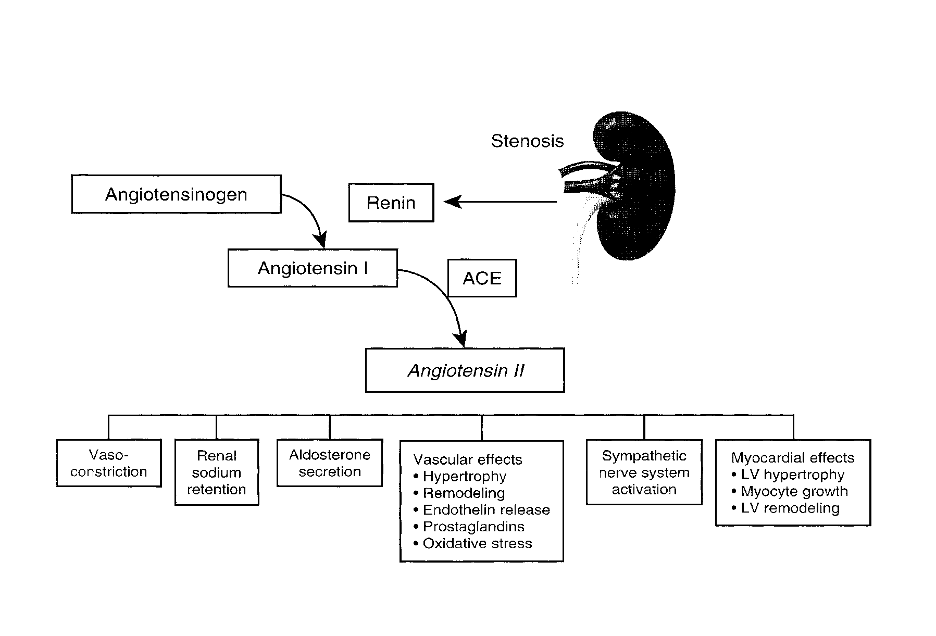
\includegraphics[width=13in]{images/renal1}

\textbf{I think the flow limitation part has been well established. What
next?}

Renal (especially bilateral) hypoperfusion induces activation of the
renin-angiotensin-aldosterone system which increases vascular tone and
impairs sodium excretion resulting in expansion of the extracellular
fluid volume.

\hypertarget{medical-management-and-evaluation}{%
\section{Medical Management and Evaluation}\label{medical-management-and-evaluation}}

\textbf{Can't we just treat their hypertension and give these patients an ACE
inhibitor at this point?}

Sure. And oftentimes we do. In fact, many of these patients can be
treated with medical therapy without loss of function or irreversible
fibrosis, sometimes for many years

\begin{itemize}
\item
  Studies in human subjects demonstrate that, despite a moderate
  reduction in renal perfusion pressure (up to 40 \%) and in renal
  blood flow (mean 30 \%), glomerular filtration is reduced but tissue
  oxygenation within the kidney cortex and medulla can adapt without
  the development of severe hypoxia.
\item
  But this only works to an extent.
\end{itemize}

\textbf{Explain that\ldots{}}

As the hypertension is treated, we're lowering the pressure gradient
across the stenosis and can actually increase the degree of renal
malperfusion and worsen the renal function.

\begin{itemize}
\tightlist
\item
  Oftentimes this loss of kidney function is a reversible consequence
  of antihypertensive therapy but it to some degree limits our ability
  to control the hypertension medically without causing further damage
  to the kidneys\ldots. And it can also reflect progressive narrowing of
  the renal arteries and/or progressive intrinsic kidney disease as
  more advanced vascular occlusion, corresponding to a 70 to 80\%
  narrowing of the renal artery, leads to demonstrable cortical
  hypoxia.
\end{itemize}

\textbf{Can we tell who has cortical hypoxia through diagnostic tests?}

A: To some degree. Cortical perfusion can be measured by blood oxygen
level dependent magnetic resonance (BOLD-MR). Additionally, inflammatory
markers sampled from renal veins of stenotic kidneys correlated strongly
with the degree of hypoxia (as measured by BOLD-MR), particularly after
correction of the stenosis with angioplasty

\textbf{So we have a patient with evidence of malperfused kidneys, either
through worsening renal function or uncontrolled hypertension, with
known discrete stenoses, and we even got a BOLD-MRI which confirms it.
Let's just revascularize them and be done with it?}

Not so fast. Although vascular stenosis or occlusion can initiate these
processes, long-standing ischemia causes parenchymal injury
characterized by inflammation and fibrosis which eventually becomes an
irreversible process. At some point, restoring renal blood flow provides
no recovery of kidney function or clinical benefit.

\textbf{So how can we determine who has CKD or hypertension due to
renovascular stenosis that we can actually help?}

This is probably the most important question since in this whole disease
process.

\begin{itemize}
\tightlist
\item
  To start, if a patient has the clinical manifestations of ischemic
  nephropathy or renovascular hypertension as we discussed above, a
  presumptive diagnosis of ischemic nephropathy can be made if there
  is radiologic documentation of significant stenosis (usually more
  than 70 \% luminal occlusion) of both renal arteries or of one renal
  artery to a solitary functioning kidney.
\end{itemize}

\textbf{But how do we know the vascular occlusive disease posing critical
hemodynamic limitation to kidney function?}

\begin{itemize}
\item
  Generally, luminal occlusion of at least 60 to 75 \% is required to
  limit blood flow and reduce perfusion pressure
\item
  This degree of stenosis is usually associated with a measurable
  translesional ``pull-back'' pressure gradient of 10 to 15 mmHg.
\item
  Doppler ultrasound criteria \citep{hoffmannRoleDuplexScanning1991, zierlerStrandnessDuplexScanning2016}

  \begin{itemize}
  \item
    Peak systolic velocities above \textgreater170 cm/sec with post stenotic
    turbulence to identify less than 60 \% luminal stenosis.
  \item
    Renal aortic ratio \textgreater3.5 required to diagnose greater than 60\%
    stenosis.
  \item
    Elevated velocities can be seen with tortuosity, but this should
    be able to be confirmed with B-mode.
  \end{itemize}
\item
  Identifiable levels of cortical hypoxia (measured by blood oxygen
  level dependent magnetic resonance BOLD-MR) are usually associated
  with translesional velocities above 385 cm/sec or reduction of
  single kidney glomerular filtration rate (GFR) in the range of 20 to
  25 mL/min.
\item
  MRA can be used for evaluation

  \begin{itemize}
  \item
    Pro - no radiation, good imaging of distal renal arteries, no
    degradation from ostial calcium.
  \item
    Cons - requires GAD -\textgreater{} interstitial fibrosis in CKD
    \[@galanNephrogenicSystemicFibrosis\] and degrades with motion
    and respiration
    \citep{nelsonGadoliniumenhancedBreathholdThreedimensional1999}
  \end{itemize}
\end{itemize}

\textbf{Most importantly: is the condition of the kidneys such that restoring
renal blood flow is likely to benefit function?}

Short answer, we still can't be certain.

Long answer, we can at least have some idea by considering the renal
resistive index, the six-month trajectory of kidney function, and the
size of the kidneys or by performing a kidney biopsy (which is not
usually done).

\begin{itemize}
\item
  None of these factors predict the outcome of revascularization with
  certainty.
\item
  \uline{Improved and validated methods to evaluate the salvageability of
  kidney function in this disorder are greatly needed and are the holy
  grail of this disease process.}
\end{itemize}

\textbf{Let's go through some of these:}

\uline{Renal Resistive index:}

Some studies indicate that elevated resistive indices in segmental
vessels (above 0.80) measured by duplex ultrasound denote poor prognosis
for renal recovery while a low resistive index is a favorable sign.

\uline{Trajectory of kidney function}

The most consistent predictor of good recovery of kidney function after
revascularization has been a recent deterioration of kidney function
(ie, in the prior six to twelve months).

\uline{Kidney size}

Very small kidneys (less than 7 cm in longest diameter) are usually
considered unlikely to recover after revascularization.

\uline{Kidney biopsy}

Previous studies suggest that biopsy demonstrating preexisting
atheroembolic changes and interstitial fibrosis indicate a limited
potential for recovery.

\begin{itemize}
\tightlist
\item
  Biopsies are not usually performed.
\end{itemize}

\uline{Comparison of kidney morphology with kidney function}

Some investigators have recommended assessing morphologic parameters,
such as renal parenchymal volume and cortical thickness with MRI, and
comparing these parameters with kidney function measured by radionuclide
scanning

\begin{itemize}
\tightlist
\item
  In a stenotic kidney, apparently normal morphology combined with
  reduced function may indicate a ``hibernating kidney'' that could be
  salvaged with revascularization.
\end{itemize}

\textbf{So how do we get a definitive diagnosis?}

A definitive diagnosis is not usually made before revascularization. In
practice, confirmation of the diagnosis is based upon stabilization or
improvement of the GFR after successful revascularization.

\hypertarget{operative-managment}{%
\section{Operative Managment}\label{operative-managment}}

\textbf{Now we think our patient's renal artery stenosis maybe is causing
hypertension or decline in renal function and we can possibly reverse
it\ldots{} how do we treat it?}

For starters, all of these patients should receive medical therapy to
control their hypertension in addition to routine CKD care and
surveillance. They need to be aggressively treated for secondary
prevention of cardiovascular morbidity with aspirin, statins, cessation
of smoking, and, in patients with diabetes, glycemic control.

\textbf{Second, once diagnosis has been made we have 2 therapeutic
alternatives\ldots{} Which are?}

First, medical therapy alone- this generally involves ACE-I or ARB and
as we discussed.

RAS can worsen ACE-I and ARB induced renal dysfunction due to systemic
hypotension, efferent arterial vasodilation, and reduced glomerular
hydrostatic pressure, in turn lowering GFR.
{[}\citep{rickey125RenovascularDisease2019, schoolwerthRenalConsiderationsAngiotensin2001}{]}

\textbf{Okay, in other words we can have chronic normalization of the systemic
pressure that might eventually lead to ischemic atrophy due to the
reduced renal perfusion pressure distal to the stenosis? Any other
concerns with medical management alone?}

\begin{itemize}
\tightlist
\item
  We're addressing or prevention progression of stenosis in those with
  atherosclerotic disease.
\end{itemize}

\textbf{Since this isn't a vascular medicine podcast, what's our other
option?}

Procedural intervention (open or endovascular) along with medical
therapy.

\textbf{Now you're talking. Who should we fix operatively?}

Some but not all patients should undergo revascularization, Patient
selection single most important factor.

Depends upon the hemodynamic severity and likely recoverability of
kidney function

\textbf{You mentioned recoverability before, can you once again touch on some
recoverability indicators?}

\begin{itemize}
\item
  A short duration of blood pressure elevation prior to the diagnosis
  of renovascular disease, since this is the strongest clinical
  predictor of a fall in blood pressure after renal revascularization
\item
  Failure of optimal medical therapy to control the blood pressure
\item
  Intolerance to optimal medical therapy (eg, deterioration of renal
  function during antihypertensive drug therapy)
\item
  Recurrent flash pulmonary edema and/or refractory heart failure
\item
  Otherwise unexplained progressive renal insufficiency, particularly
  if proteinuria is absent
\item
  CKD stage 3a and 3b most likely to benefit from revascularization.
  \citep{singerImpactBaselineRenal2009}

  \begin{itemize}
  \tightlist
  \item
    Lower GFR likely to progress to ESRD
  \end{itemize}
\item
  Degree of stenosis, age, pre-procedure BP control and meds are not
  assocaited with improvement.
  \citep{textorPercutaneousRevascularizationIschemic2013}
\end{itemize}

\textbf{But do we have any good data proving our interventions help?}

This is where things can get muddy.

Early on, observational studies demonstrated a high rate of procedural
success with percutaneous transluminal renal angioplasty (PTRA) and
stent placement (\textasciitilde85\%) in patients with ostial atherosclerotic disease,
as well as a high rate of clinical success measured by improvements in
blood pressure and kidney function in 50 to 75 \% of subjects.

\textbf{Anything better than observational studies?}

Unfortunately, randomized trials showed no additional benefit from
stenting when added to medical therapy with respect to blood pressure
control, renal function, cardiovascular events, and mortality. But these
studies have their own limitations.

\textbf{The one we keep hearing about is the CORAL trial. Tell me about
that.}

\begin{itemize}
\item
  CORAL trial \citep{cooperStentingMedicalTherapy2014}

  \begin{itemize}
  \item
    Cardiovascular Outcomes in Renal Atherosclerotic Lesions (CORAL)
    trial
  \item
    947 patients (80 \% had unilateral disease) who met the following
    two criteria:

    \begin{itemize}
    \item
      Unilateral or bilateral atherosclerotic renal artery
      stenosis \textgreater60 \% if diagnosed with conventional angiography,
      peak systolic velocity \textgreater300 cm/second if diagnosed by
      duplex Doppler ultrasonography, Luminal narrowing \textgreater80 \% if
      diagnosed with magnetic resonance angiography or
      computerized tomography angiography (or \textgreater70 \% with
      additional evidence of renal ischemia)
    \item
      Systolic hypertension despite two or more antihypertensive
      medications and/or an estimated glomerular filtration rate
      (eGFR) \textless60 mL/min/1.73 m2 that was presumably due to the
      stenosis.
    \item
      All patients received antiplatelet therapy plus best medical
      therapy including ARB
    \end{itemize}
  \item
    Revascularization had no additional effect on the primary
    outcome (a composite of cardiovascular or renal death, stroke,
    myocardial infarction, hospitalization for heart failure, a
    reduction in eGFR by more than 30 \%, or end-stage renal disease)
    as compared with medical therapy alone (35.1 versus 35.8 \%).
  \item
    No effect on any of the individual components of the primary
    outcome.
  \item
    Low procedural complication rate \textasciitilde2\%
  \item
    Similar findings in the ASTRAL trial
    \citep{astralinvestigatorsRevascularizationMedicalTherapy2009}
  \end{itemize}
\end{itemize}

\textbf{Well, that sounds pretty convincing.}

\begin{itemize}
\item
  Limitations on existing treatment data:

  \begin{itemize}
  \item
    \uline{Considerable selection bias} -- For the most part,
    the patients enrolled in these trials did \textbf{not} meet the
    criteria for selecting patients likely to benefit from
    intervention (eg, short duration of blood pressure elevation,
    hypertension resistant to medical therapy, recurrent flash
    pulmonary edema):

    \begin{itemize}
    \item
      CORAL \citep{cooperStentingMedicalTherapy2014}

      \begin{itemize}
      \item
        Patients hospitalized for heart failure within 30 days
        of screening for the trial were excluded, thereby
        limiting the number of trial participants with recurrent
        flash pulmonary edema.
      \item
        Mean number of antihypertensive medications used by
        CORAL participants at baseline was 2.1- many had not
        failed optimal medical therapy
      \item
        More than 25 \% had controlled blood pressure upon entry
        into the trial.
      \item
        Mortality and event rates lower than in most previous
        registries, suggesting that many high-risk patients were
        not enrolled.
      \end{itemize}
    \item
      ASTRAL
      \citep{astralinvestigatorsRevascularizationMedicalTherapy2009}

      \begin{itemize}
      \tightlist
      \item
        Large number of patients had stenoses that were probably
        not clinically significant (50 to 70 \%), and patients
        were excluded if their primary doctors felt that they
        ``definitely'' needed revascularization.
      \end{itemize}
    \end{itemize}
  \item
    \uline{Results of the trials differ substantially from observational
    reports of ``high-risk'' subsets}

    \begin{itemize}
    \tightlist
    \item
      For the most part, patients selected by their treating
      clinicians to undergo revascularization have derived greater
      benefit from revascularization than did patients enrolled in
      the trials who were randomly assigned to revascularization
    \end{itemize}
  \end{itemize}
\end{itemize}

\hypertarget{endovascular-therapy}{%
\subsection{Endovascular Therapy}\label{endovascular-therapy}}

\textbf{We've determined our patient is an appropriate candidate for
intervention, and we don't fully buy into CORAL, what can we do?}

\begin{itemize}
\item
  \uline{Percutaneous renal angioplasty/stenting}in addition to
  medical therapy

  \begin{itemize}
  \item
    Most commonly employed if technically feasible.
  \item
    Most amenable lesions to angioplasty are those producing
    incomplete occlusion in the main renal artery.

    \begin{itemize}
    \tightlist
    \item
      Total occlusions and ostial lesions extending into aorta
      generally do not respond well to angioplasty alone due to
      elastic recoil.
    \end{itemize}
  \item
    Quick results: maximum antihypertensive response is generally
    observed at 48 hours after the procedure

    \begin{itemize}
    \tightlist
    \item
      But BP levels and antihypertensive drug requirements often
      change over subsequent weeks
    \end{itemize}
  \item
    In general, the effects of revascularization on blood pressure
    were greater in bilateral disease, but effects on renal function
    and mortality did not differ in those with bilateral as compared
    with unilateral stenosis .
  \item
    Most atherosclerotic lesions are now treated with primary
    stenting to avoid rapid development of restenosis.

    \begin{itemize}
    \item
      A higher initial primary success rate, defined as less than
      50 \% stenosis (88 versus 57 \%).
    \item
      At six months, a higher patency rate (75 versus 29 \%) and a
      lower restenosis rate (14 versus 48 \%).
    \item
      Twelve patients assigned to PTRA alone underwent stenting
      because of treatment failure within six months. These
      patients had a similar blood pressure response as those
      initially treated with stenting.
    \end{itemize}
  \item
    Performing a renal angiogram
    \citep{edwards127RenovascularDisease2019}

    \begin{enumerate}
    \def\labelenumi{\arabic{enumi}.}
    \item
      Supine with arms overhead or straight out to the sides
    \item
      LAO 15-20deg
    \item
      Flush catheter placed just above the renals
    \item
      Breath hold, high frame rate and non-DSA due unavoidable
      patient movement
    \end{enumerate}
  \end{itemize}
\end{itemize}

\textbf{What about complications?}

\begin{itemize}
\item
  Complication rate with percutaneous transluminal renal angioplasty
  with or without stenting is between 5 and 15 \%

  \begin{itemize}
  \item
    Mostly minor: puncture site hematoma and renal artery
    dissection.
  \item
    Serious complications more rare: renal artery thrombosis or
    perforation, AKI 2/2 atheroembolic disease (\textasciitilde1\%)or
    radiocontrast agent injury.
  \item
    Mortality exceedingly rare
  \end{itemize}
\end{itemize}

\textbf{Outcomes data}

\begin{itemize}
\item
  In the correct patient population:

  \begin{itemize}
  \item
    Unilateral disease

    \begin{itemize}
    \item
      PTRA alone results in normalization of blood pressure
      (removal of antihypertensive drug therapy) \textasciitilde8-20\%
    \item
      Some improvement 50-60\%
    \item
      Failure rate \textasciitilde20-30\%
    \item
      Restenosis rate of 8 to 30 \% at two years (without stent)
    \item
      Better results with unilateral fibromuscular disease.
    \item
      Less consistent for patients with chronic hypertension
      compared with patients who have an acute elevation in blood
      pressure
    \end{itemize}
  \item
    Bilateral disease

    \begin{itemize}
    \item
      25-30\% will recover kidney function to a meaningful degree,
      sometimes avoiding progression to end-stage kidney disease
      (ESKD) and/or the need for renal replacement therapy.
    \item
      \textasciitilde50\% will have little immediate change in kidney function
      but will ``stabilize''
    \item
      \textasciitilde20\% will have a progressive deterioration of kidney
      function, sometimes related to the procedure
    \end{itemize}
  \end{itemize}
\end{itemize}

\textbf{Guidelines}

\begin{itemize}
\item
  2005 ACC/AHA guidelines on peripheral artery disease recommends that
  a stent be placed in patients undergoing PTRA for treatment of
  atherosclerotic renal artery stenosis \citep{hirschACCAHA20052006}

  \begin{itemize}
  \item
    PTRA without stent placement is rarely performed unless the
    anatomy precludes stenting.
  \item
    POBA without stenting is generally less successful and
    associated with more complications (eg atheroemboli)
  \end{itemize}
\end{itemize}

\textbf{How durable is PTA/stenting?}

\begin{itemize}
\item
  Restenosis

  \begin{itemize}
  \item
    \textasciitilde11-17\%

    \begin{itemize}
    \tightlist
    \item
      11-39\% during the first one to two years
    \end{itemize}
  \item
    Detected as a rise in blood pressure requiring more intensive
    therapy
  \item
    Angioplasty/stenting injures the vascular endothelium, which may
    result in restenosis.
  \item
    Symptomatic stenosis leading to a rise in blood pressure or a
    fall in GFR are less common and are reported in 10 to 20 \% of
    patients
  \end{itemize}
\end{itemize}

\textbf{How do you follow these patients after stenting?}

\begin{itemize}
\item
  Follow-up of patients who have had a renal artery stent should
  include serial measurements of blood pressure and estimation of GFR.

  \begin{itemize}
  \item
    Post-stent duplex ultrasound @2-4weeks with
  \item
    Repeated examinations on a quarterly basis (not much data)
  \item
    Patients who develop an increase in pressure or reduced GFR
    after stenting should undergo duplex ultrasonography to identify
    restenosis
  \item
    Retreatment with angioplasty with or without repeat stenting can
    be attempted, but the restenosis rate after repeat angioplasty
    is increased.

    \begin{itemize}
    \tightlist
    \item
      Surgical reconstruction may be pursued in patients with
      recurrent episodes of restenosis and loss of kidney
      function.
    \end{itemize}
  \end{itemize}
\end{itemize}

\hypertarget{open-surgery}{%
\subsection{Open Surgery}\label{open-surgery}}

\textbf{What about an open operation?}

\begin{itemize}
\item
  \uline{Surgical revascularization} used in addition to medical
  therapy

  \begin{itemize}
  \tightlist
  \item
    Less common since the widespread application of effective
    antihypertensive drug therapy and endovascular stents (mid 90s)
  \end{itemize}
\end{itemize}

\textbf{So who still gets open repair?} \citep{benjamin126RenovascularDisease2019}

\begin{itemize}
\tightlist
\item
  Younger patients
\item
  Unfavorable anatomy (i.e.~occlusion or branch disease)
\item
  Failures of endovascular therapy (i.e.~in stent restenosis)
\item
  Need for concomittent aortic revascularization.
\end{itemize}

\textbf{How do we do it?}

\begin{itemize}
\item
  Involves bypassing the stenotic segment or of removing a small
  atrophic kidney with nearly complete arterial occlusion.

  \begin{itemize}
  \item
    From the aorta or hepatorenal or splenorenal bypass to avoid
    diseased aorta.
  \item
    Bilateral: either bilateral repair or unilateral repair with
    contralateral nephrectomy of a nonfunctioning, atrophic kidney.
  \end{itemize}
\item
  Bilateral ostial disease in a young patient can be treated with
  transverse arteriotomy and bilateral renal endarterectomy. Close
  primarily or with PTFE/polyester patch. Second line is bilateral
  bypass with GVS. \citep{benjamin126RenovascularDisease2019}
\end{itemize}

\textbf{How do outcomes compare to PTA/stenting?}

\begin{itemize}
\item
  Equally or more effective than PTRA in the treatment of
  atherosclerotic disease, with cure of or improvement in the
  hypertension occurring in 80 to 95 \% of patients.

  \begin{itemize}
  \tightlist
  \item
    Cure of hypertension after surgery is most likely in patients
    who have been hypertensive for less than five years
  \end{itemize}
\item
  Lack of complete response was usually associated with one of two
  factors:

  \begin{itemize}
  \item
    Presence of underlying primary/essential hypertension
  \item
    Development of intrarenal vascular disease due to exposure of
    the contralateral kidney to the elevated blood pressure.
  \end{itemize}
\end{itemize}

\textbf{Guidelines recommendations?}

\begin{itemize}
\item
  2005 American College of Cardiology/American Heart Association
  (ACC/AHA) guidelines \citep{hirschACCAHA20052006}

  \begin{itemize}
  \tightlist
  \item
    Open surgery in patients with atherosclerotic renal artery
    stenosis largely restricted to those who have multiple small
    renal arteries, have early primary branching of the main renal
    artery, require aortic reconstruction near the renal arteries
    for other indications (eg, aneurysm repair or severe aortoiliac
    occlusive disease), or to avoid manipulation of a highly
    diseased aorta or failed endovascular stents (using specific
    surgical techniques, including splenorenal, ileorenal, or
    hepatorenal bypass procedures).
  \end{itemize}
\end{itemize}

\textbf{So why not do it instead of stent?}

\begin{itemize}
\item
  In-hospital mortality: \textasciitilde3-10 \% in high volume centers

  \begin{itemize}
  \item
    Risk factors diffuse atherosclerosis, advanced age, chronic
    kidney disease, heart failure, or chronic lung disease.
  \item
    No deaths in 105 procedures for fibromuscular dysplasia (FMD).
  \end{itemize}
\end{itemize}

\hypertarget{fibromuscular-dysplasia-fmd}{%
\section{Fibromuscular Dysplasia (FMD)}\label{fibromuscular-dysplasia-fmd}}

\textbf{You mentioned FMD as a cause of renovascular hypertension, tell me
more about that\ldots{}}

Fibromuscular dysplasia (FMD) is a noninflammatory, nonatherosclerotic
disorder that leads to arterial stenosis, occlusion, aneurysm,
dissection, and arterial tortuosity.

\begin{itemize}
\tightlist
\item
  Virtually always diagnosed radiographically -- formerly
  pathologically, but rarely sent for specimen in modern diagnosis or
  treatment
\end{itemize}

\textbf{How do we classify it?}

\begin{itemize}
\item
  Most commonly classified by angiographic appearance:

  \begin{itemize}
  \item
    Multifocal FMD (more common)

    \begin{itemize}
    \item
      angiographic appearance of a ``string of beads.''
    \item
      corresponds pathologically to medial fibroplasia, the most
      common histologic type, and to perimedial fibroplasia, which
      is less common.
    \end{itemize}
  \item
    Focal FMD (less common)

    \begin{itemize}
    \item
      angiographic appearance of a ``circumferential or tubular
      stenosis''
    \item
      corresponds pathologically to intimal fibroplasia but medial
      hyperplasia and periarterial hyperplasia may also have a
      focal appearance.
    \end{itemize}
  \item
    These two different angiographic subtypes of FMD (multifocal and
    focal) have different phenotypic presentations and natural
    history

    \begin{itemize}
    \tightlist
    \item
      Is FMD is, in fact, a single disease?
    \end{itemize}
  \end{itemize}
\end{itemize}

\textbf{Where does it occur?}

\begin{itemize}
\item
  Has been observed in nearly every arterial bed
\item
  Involvement of the renal arteries \textasciitilde75-80\%
\item
  Involvement of the extracranial cerebrovascular arteries (eg,
  carotid and vertebral arteries) \textasciitilde75\%

  \begin{itemize}
  \tightlist
  \item
    2/3 of patients have multiple arteries involved.
  \end{itemize}
\end{itemize}

\textbf{Who has FMD?}

\begin{itemize}
\item
  \textasciitilde90\% of cases in adults are in women.

  \begin{itemize}
  \tightlist
  \item
    No female predominance among children with FMD.
  \end{itemize}
\item
  Mean age at diagnosis was 52 years, with a range of 5 to 86 years

  \begin{itemize}
  \tightlist
  \item
    In the past, it was believed that FMD was a disease of young
    women. However, older now know to make up a large proportion of
    affected
  \end{itemize}
\item
  35-50\% of cases in children and 5-10\% of cases in adults under the
  age of 60 years with renovascular hypertension
\item
  Often an incidental finding:

  \begin{itemize}
  \item
    4.4\% of potential kidney donors had evidence of FMD.
  \item
    CORAL trial:

    \begin{itemize}
    \tightlist
    \item
      FMD was discovered in 5.7\% of the total study population
      (8.8\% of enrolled females)
    \end{itemize}
  \end{itemize}
\end{itemize}

\textbf{What causes FMD?}

The exact etiology of FMD remains unknown, but some mechanisms have been
proposed

\begin{itemize}
\item
  Most often results from medial fibroplasia (60-90\% of cases).
  Collagen deposits in the media result in elastic fibrils and
  fibromuscular ridges. \citep{olinFibromuscularDysplasiaState2014}
\item
  'Genetics may play an important role in development

  \begin{itemize}
  \item
    Some studies report autosomal mode of inheritance with variable
    penetrance
  \item
    Potential association with a single nucleotide variant in the
    phosphatase and actin regulator 1 gene (PHACTR1)
  \item
    Variant rs9349379 is also a risk locus for coronary artery
    disease, migraine headache, and cervical artery dissection.
  \end{itemize}
\item
  Predominance of young/childbearing age women hormonal influences are
  thought to play a role

  \begin{itemize}
  \tightlist
  \item
    Remains unproven.
  \end{itemize}
\item
  Mechanical factors such as stretch and trauma unproven.
\end{itemize}

\textbf{Does FMD present differently that the atherosclerotic renovascular
disease we talked about?}

\begin{itemize}
\item
  Varies widely depending on artery affected and as it results from:
\item
  Ischemia related to stenosis
\item
  Dissection and occlusion of major arteries (renal infarction,
  stroke, myocardial infarction)
\item
  Rupture of aneurysms
\item
  Embolization of intravascular thrombi from dissection or aneurysms
\end{itemize}

\textbf{What are the common presenting symptoms and signs}

\begin{itemize}
\item
  Manifestations of renal FMD (eg, hypertension, flank pain) are more
  likely to occur in men, as are arterial dissections and aneurysms.

  \begin{itemize}
  \item
    Most common presenting signs:
  \item
    Hypertension -- 67\% (66\% of women and 74 \% of men)
  \end{itemize}
\item
  But overall hypertension is the most common manifestation of renal
  artery FMD in both genders

  \begin{itemize}
  \tightlist
  \item
    Flank pain and abdominal pain can result from ischemia, aneurysm
    rupture, or dissection of renal and mesenteric arteries,
    respectively.
  \end{itemize}
\end{itemize}

\textbf{Are these dissections common?}

\begin{itemize}
\item
  High prevalence of aneurysm and/or dissection

  \begin{itemize}
  \item
    Aneurysm (22\%) and dissection (26\%).

    \begin{itemize}
    \item
      34\% of aneurysms were renal
    \item
      11\% of dissections were renal
    \end{itemize}
  \item
    42\% had an aneurysm and/or dissection.
  \end{itemize}
\end{itemize}

\textbf{So should we screen for these dissections in a patient with known
FMD?}

\begin{itemize}
\item
  Every patient diagnosed with FMD should have one-time,
  head-to-pelvic CTA (or MRA) is an alternative.

  \begin{itemize}
  \tightlist
  \item
    CTA of the neck and head on one day followed one week later by
    CTA of the chest, abdomen, and pelvis
  \end{itemize}
\end{itemize}

\textbf{When should we suspect FMD?}

\begin{itemize}
\item
  Hypertension (particularly in a woman under the age of 60 years)
  with findings that would prompt an evaluation for secondary
  hypertension:

  \begin{itemize}
  \item
    Severe or resistant hypertension.
  \item
    Onset of hypertension before the age of 35 years.
  \item
    A sudden rise in blood pressure over a previously stable
    baseline.
  \item
    A significant increase in the serum creatinine concentration
    after the institution of therapy with an angiotensin-converting
    enzyme (ACE) inhibitor or angiotensin receptor blocker (ARB) in
    the absence of an excessive reduction in blood pressure.
  \item
    An epigastric/abdominal bruit.
  \end{itemize}
\item
  Renal artery dissection (or carotid, vertebral, coronary)
\item
  Aneurysm in a visceral, carotid, vertebral, or intracranial vessel.
\item
  Renal infarction.
\end{itemize}

\textbf{How do we diagnose this and/or distinguish it from renovascular
atherosclerotic disease?}

\begin{itemize}
\item
  Confirmed by diagnostic imaging that reveals consistent findings
\item
  Noninvasive imaging test is usually performed first. This includes
  CTA, MRA, and Duplex ultrasound.
\end{itemize}

\textbf{Let talk about CTA\ldots{}}

\begin{itemize}
\item
  CTA is preferable due to higher spatial resolution than MRA, less
  dependence upon technical expertise, and a shorter scan time
\item
  Excellent diagnostic accuracy for FMD of the main renal arteries,
  although the sensitivity decreases when FMD is only present in the
  smaller branch renal arteries.
\item
  Multirow detector CT scanners, which offer more rapid image
  acquisition, variable section thickness, three-dimensional
  rendering, diminished helical artifacts, and smaller contrast
  requirements, may gain an increased role in the diagnosis and
  follow-up of renal artery FMD
\end{itemize}

\textbf{What about MRA?}

\begin{itemize}
\item
  Inconsistent detection of FMD and is performed if CTA is
  contraindicated
\item
  The spatial resolution in the branch vessels is not adequate, and
  artifact may occur, suggesting ``beading'' when none is present.
\item
  May miss mild FMD.
\item
  Can be useful for detecting aneurysms and dissections
\end{itemize}

\textbf{And finally, Duplex ultrasonography}

\begin{itemize}
\item
  Detects elevated blood flow velocities in the mid and distal
  portions of the renal artery, most common locations for FMD.
\item
  Increased peak systolic velocity, turbulent blood flow, and
  tortuosity of the mid and distal artery.

  \begin{itemize}
  \tightlist
  \item
    \% diameter stenosis reports less helpful and usually inaccurate
  \end{itemize}
\item
  lowest spatial resolution of all of the cross-sectional imaging
  modalities
\item
  most operator dependence
\item
  first choice only in high-volume centers with extensive expertise in
  this technique
\end{itemize}

\textbf{What about non invasive testing?}

\begin{itemize}
\item
  DSA is performed in patients if there is a high clinical suspicion
  of FMD, and treatment with revascularization is planned if a
  stenosis is found.

  \begin{itemize}
  \item
    Can improve visualization of the arteries by eliminating
    background soft tissue and bone and has higher spatial
    resolution than any of the other imaging modalities
  \item
    Can measure the pressure gradient across the stenosis

    \begin{itemize}
    \item
      Pressure decrease threshold of 10 \% or more of the mean
      pressure should be used to decide whether a lesion is
      hemodynamically significant
    \item
      IVUS and optical coherence tomography (OCT) can be helpful
      in determining if a dissection or intramural hematoma is
      present as well as help to determine if angioplasty has
      improved the stenosis.
    \end{itemize}
  \item
    Negative DSA excludes a diagnosis of FMD in the vascular bed
    that was imaged.
  \end{itemize}
\end{itemize}

\textbf{Any place for pathologic diagnosis in modern therapy?}

\begin{itemize}
\item
  Histopathology (and histologic classification) is \textbf{no longer} part
  of the diagnosis.

  \begin{itemize}
  \tightlist
  \item
    Only in the rare patient who requires surgical revascularization
    or resection of an aneurysm.
  \end{itemize}
\end{itemize}

\textbf{So how do we treat this, what warrants intervention and are those
interventions different than what we offer atherosclerotic disease of
the renal arteries?}

\begin{itemize}
\item
  All patients with FMD should be placed on antiplatelet therapy (ASA)
  unless otherwise contraindicated
\item
  \uline{Antihypertensive therapy}

  \begin{itemize}
  \item
    Most patients will require antihypertensive therapy, even if
    they undergo revascularization.
  \item
    Majority of patients with \textbf{focal} FMD have their blood
    pressure cured with angoplasty
  \end{itemize}
\end{itemize}

\textbf{But what about revascularization?}

\begin{itemize}
\item
  \uline{Revascularization} Goal: control of hypertension

  \begin{itemize}
  \item
    BP can be controlled in most adults with multifocal FMD with a
    mean of two antihypertensive medications
  \item
    Weigh risks and benefits in well controlled hypertension.
  \end{itemize}
\item
  \textbf{No} randomized trials comparing revascularization with medical
  therapy
\end{itemize}

\textbf{Well then who do we treat?}

\begin{itemize}
\item
  Recent-onset hypertension, with goal to cure hypertension.
\item
  Resistant hypertension despite compliance with an appropriate
  three-drug regimen.
\item
  Patients unable to tolerate antihypertensive medications or who are
  noncompliant with their medication regimen.
\item
  Adults with bilateral renal FMD, or unilateral renal FMD to a single
  functioning kidney, and unexplained progressive renal insufficiency
  thought to result from renal artery stenosis
\item
  Hypertensive children.
\item
  may be at higher risk than adults for progressive renal parenchymal
  loss, and therefore could benefit from revascularization even if
  their hypertension can be well-controlled with one or two
  antihypertensive medications.
\end{itemize}

\textbf{And what kind of results do we get with revascularization?}

\begin{itemize}
\item
  Hypertension is cured or improved following revascularization in a
  large proportion of patients with FMD.

  \begin{itemize}
  \item
    Much better than 2/2 atherosclerosis
  \item
    Varies considerably from study to study, although hypertension
    control improves in most patients and depends in large part upon
    the definition of cure.
  \item
    Not good data on stabilization of either GFR or renal size in
    patients with FMD.
  \end{itemize}
\end{itemize}

What options do we have in terms of revascularization?

\textbf{Angioplasty and open surgery}

Do we have good results treating FMD with these?

\begin{itemize}
\item
  Patients most often treated with angioplasty alone with good
  success. \citep{daviesLongtermOutcomesPercutaneous2008, jenkinsOutcomesHypertensivePatients2015}
\item
  Improvement in blood pressure (including those with and without
  cure) was similar with PTA as compared with surgery (86 versus 88
  \%).
\item
  Older age and longer duration of hypertension prior to
  revascularization were significantly associated with a lower cure
  rate.
\end{itemize}

\textbf{How do these compare?}

\begin{itemize}
\item
  PTA achieves similar technical success and is associated with a
  lower risk of adverse events in observational studies
\item
  Most patients with FMD who are selected for renal revascularization
  have PTA rather than surgery
\item
  Major adverse events were more frequent with surgery (15 versus 6
  \%).
\end{itemize}

\textbf{So why choose open surgery?}

\begin{itemize}
\item
  Cure rates were higher with surgery (54 versus 36 \%).
\item
  Surgery rather than PTA if PTA fails or if the arterial anatomy is
  not amenable to PTA

  \begin{itemize}
  \tightlist
  \item
    Patients with small renal arteries (\textless4 mm), with branch renal
    artery disease, or with extensive intimal fibroplasia.
  \end{itemize}
\end{itemize}

\textbf{So how do we perform Percutaneous transluminal angioplasty} for FMD?

\begin{itemize}
\tightlist
\item
  \uline{Without} stent placement\ldots{} unlike PTA for
  atherosclerotic RAS
\end{itemize}

\textbf{Why not place a stent?}

\begin{itemize}
\item
  Patients do very well with angioplasty alone, no reason to place a
  stent.

  \begin{itemize}
  \item
    Lesion is so fibrotic that the pressure gradient cannot be
    obliterated with an angioplasty, a stent will not correct this
    problem

    \begin{itemize}
    \tightlist
    \item
      Such patients should be referred for surgery.
    \end{itemize}
  \end{itemize}
\item
  Usually have stenoses in the mid and distal portions of the artery
  rather than at the ostium or proximal portion (as occurs with
  atherosclerosis).

  \begin{itemize}
  \tightlist
  \item
    Should surgical revascularization become necessary due, for
    example, to in-stent restenosis, patients may require more
    complex branch repair to bypass the occluded stent since the
    stent often covers the renal artery up to the point of the first
    intrarenal branch.
  \end{itemize}
\end{itemize}

\textbf{Do we ever place stents?}

\begin{itemize}
\tightlist
\item
  Stents placed when a dissection results from the performance of PTA
  or in the rare instance in which a perforation of the renal artery
  occurs during angioplasty.
\end{itemize}

\textbf{And we're getting good outcomes with PTA alone?}

\begin{itemize}
\item
  Technical (angiographic) success rates for PTA 83-100
\item
  Rate of restenosis 12-34\% over follow-up intervals of six months to
  two years

  \begin{itemize}
  \item
    Difficult to determine if patients with FMD develop restenosis,
    or if the lesion was not completely treated correctly the first
    time.
  \item
    Not necessarily associated with recurrent hypertension.
  \end{itemize}
\end{itemize}

\textbf{But generally we can achieve significant and sustained reductions in
systolic blood pressure, diastolic blood pressure, serum creatinine, and
number of antihypertensive agents.}

\begin{itemize}
\tightlist
\item
  Systolic blood pressure response was better in patients with FMD
  affecting the main renal artery than in patients with branch vessel
  involvement.
\end{itemize}

\textbf{Any specific technical tips?}

\begin{itemize}
\item
  Cutting balloon angioplasty should be avoided

  \begin{itemize}
  \tightlist
  \item
    Increased risk of rupture
  \end{itemize}
\item
  Post angioplasty visual inspection alone is \textbf{not} accurate.

  \begin{itemize}
  \item
    Measure pressure differential using a pressure guidewire, with a
    mean gradient of \textless5 mmHg across the treated segment suggesting
    a satisfactory result

    \begin{itemize}
    \tightlist
    \item
      Measure before and after angioplasty
    \end{itemize}
  \item
    Post-procedure renal duplex scanning

    \begin{itemize}
    \tightlist
    \item
      Degree of turbulence is less prominent, and velocity
      elevation in the mid-distal renal artery returns to normal.
    \end{itemize}
  \item
    Intravascular ultrasound or optical coherence tomography (OCT)
    is occasionally used to evaluate the elimination or reduction of
    various endoluminal defects.
  \end{itemize}
\end{itemize}

\textbf{What should we do if it doesn't work?}

\begin{itemize}
\item
  If either has no improvement in blood pressure or an initial
  improvement followed by recurrence, repeat angiogram and PTA.

  \begin{itemize}
  \tightlist
  \item
    Restenosis may actually represent inadequate angioplasty during
    the first procedure
  \end{itemize}
\item
  Persistent HTN despite technically successful PTA suggests that the
  cause of hypertension is unrelated to fibromuscular disease or is
  related to small vessel disease within the kidney (nephrosclerosis)
  due to longstanding hypertension.
\end{itemize}

\textbf{What kind of complications do we see after this?}

\begin{itemize}
\item
  Mostly related to vascular access
\item
  Rarely: renal artery perforation, dissection, or segmental renal
  infarction may occur.
\item
  Decreasing over time- 16 \% in 1998 to 3 \% in 2001
\end{itemize}

\textbf{Ok, lets switch gears to open revascularization?}

\begin{itemize}
\item
  Aortorenal bypass with a saphenous vein graft is the most common
  technique

  \begin{itemize}
  \tightlist
  \item
    Artificial graft material used occasionally
  \end{itemize}
\end{itemize}

\textbf{For everyone? What about for pediatric patients?}

\begin{itemize}
\tightlist
\item
  Pediatric patients: hypogastric artery grafts are used or else
  aortic reimplantation of the renal artery is performed because vein
  grafts become aneurysmal
\end{itemize}

\textbf{How does this compare again to PTA?}

\begin{itemize}
\item
  Similar success rates compared to PTA (82-89\% patency) but with
  higher morbidity.

  \begin{itemize}
  \item
    Perioperative mortality appears to be very low (\textasciitilde1.2\%)
  \item
    Usually limited to complex cases so success and complication
    would probably be higher if simpler cases were included.
  \end{itemize}
\end{itemize}

\textbf{What's Monitoring and follow-up look like for these patients?}

\begin{itemize}
\item
  Medical management only:

  \begin{itemize}
  \item
    Renal artery stenosis and kidney dysfunction may progress
    despite good blood pressure control

    \begin{itemize}
    \tightlist
    \item
      Mostly in patients with focal FMD and intimal fibroplasia
    \end{itemize}
  \item
    Every patient with FMD should have measurement of serum
    creatinine and renal artery duplex ultrasound every 12 months.
  \end{itemize}
\end{itemize}

\textbf{And After revascularization}?

\begin{itemize}
\item
  Duplex ultrasonography and serum creatinine measurements performed
  on the first office visit post procedure, then every six months for
  two years, and then yearly, if stable.
\item
  With worsening on new hypertension, or unexplained increase in the
  serum creatinine, he or she should be imaged at that time with
  duplex ultrasound (or CTA if the ultrasound is equivocal or poor
  quality).
\end{itemize}

\hypertarget{renal-artery-aneurysms}{%
\section{Renal Artery Aneurysms}\label{renal-artery-aneurysms}}

\textbf{Ok, that's a pretty good review, but let's switch gears and talk about
renal artery aneurysms}

\hypertarget{demographics-2}{%
\subsection{Demographics}\label{demographics-2}}

\begin{itemize}
\item
  Renal artery aneurysms are rare - Autopsy studies have revealed an
  incidence of 0.01\% to 0.09\%.
\item
  Females \textgreater{} males, although females = males with FMD excluded
\item
  Although arteriosclerotic changes have been identified in most
  aneurysms in patients with multiple lesions, this is not a uniform
  finding, suggesting that arteriosclerosis may not be the most
  important factor in the genesis of renal artery aneurysms.
\item
  More likely due to a congenital medial degenerative process with
  weakness of the elastic lamina.
\item
  Fibromuscular dysplasia (FMD) is often a direct contributor to the
  development of an aneurysm.

  \begin{itemize}
  \item
    Medial fibroplasia is typically associated with multiple
    stenoses and post-stenotic dilatation of the distal two thirds
    of the renal artery.
  \item
    Renal artery aneurysms in association with FMD are generally
    only a few millimeters in diameter.
  \item
    The typical angiographic appearance of a renal artery involved
    with medial fibroplasia is a ``string of beads.''
  \end{itemize}
\item
  A rare cause of renal artery aneurysms is Ehlers-Danlos' syndrome.

  \begin{itemize}
  \tightlist
  \item
    This disorder is associated with extreme arterial fragility and
    spontaneous rupture.
  \end{itemize}
\end{itemize}

\hypertarget{anatomy-1}{%
\subsection{Anatomy}\label{anatomy-1}}

\begin{itemize}
\item
  Most frequent site of involvement is primary bifurcation,
  intraparenchymal (\textless10\%)
\item
  Most are saccular
\item
  Right slightly more common than left, bilateral 10\%
\item
  90\% are extraparenchymal
\end{itemize}

\hypertarget{presentation-2}{%
\subsection{Presentation}\label{presentation-2}}

\begin{itemize}
\item
  Majority are associated with hypertension (70\%)
  \citep{colemanRenalArteryAneurysms2015}
\item
  10\% mortality
\item
  90\% risk of kidney loss
\item
  Less than 3\% rupture.
\end{itemize}

\hypertarget{management-10}{%
\subsection{Management}\label{management-10}}

\textbf{Size criteria currently controversial*}

\begin{itemize}
\item
  Uncontrolled hypertension is an indication for repair when smaller
  than 2.5cm. \citep{colemanRenalArteryAneurysms2015}
\item
  VLFDC recently proposed a 3cm threshold for asymptomatic renal
  artery aneurysm. \citep{klausnerContemporaryManagementRenal2015}
\item
  Many aneurysms with circumferential calcification which could offer
  protection against rupture
\end{itemize}

In an elderly patient, observation of this aneurysm with Duplex
surveillance is the appropriate treatment.

For larger aneurysms in younger patients, aneurysmorrhaphy with primary
repair or patching, interposition grafting, or bypass can be performed
with low mortality. \citep{colemanRenalArteryAneurysms2015}

\begin{itemize}
\tightlist
\item
  Comparison of ex vivo or insitu renal artery reconstruction have
  shown no difference in mortality, morbidity, LOS or reoperation.
\end{itemize}

Endovascular techniques such as coiling have been reported to be
successful in treating these saccular aneurysms; however, most aneurysms
occur at branch points making covered stent placement difficult.
\citep{colemanRenalArteryAneurysms2015}

\begin{itemize}
\tightlist
\item
  Renal artery dissection caused by guide wires or catheters can
  occur, but is rare.
\end{itemize}

\hypertarget{renal-artery-dissection}{%
\section{Renal Artery Dissection}\label{renal-artery-dissection}}

Renal ischemia if patient has new hypertension, flank pain, hematuria
and proteinuria. \citep{mullerSurgicalTreatmentRenal2003}

Endo avoided if branch involvement.

Bypass, in situ repair, auto-transplant if renal branch involvement and
possibility of renal salvage.

Nephrectomy required in uncontrolled hypertension, extensive dissection
and irreversable ischemia.

\hypertarget{renal-vein-thrombosis}{%
\section{Renal Vein Thrombosis}\label{renal-vein-thrombosis}}

\hypertarget{diagnosis-1}{%
\subsection{Diagnosis}\label{diagnosis-1}}

CT scan is best. Difficult to visualize native renal vein on duplex
imaging. \citep{asgharRenalVeinThrombosis2007, velazquez-ramirez129RenovascularDisease2019}

\hypertarget{management-11}{%
\subsection{Management}\label{management-11}}

\begin{itemize}
\item
  Renal vein thrombosis initially managed with heparin, then warfarin
  for 6mo. {[}\citep{asgharRenalVeinThrombosis2007, velazquez-ramirez129RenovascularDisease2019}{]}
\item
  Thrombectomy or thrombolysis reserved for acutely threatened kidney
  in young patient, complication of AC or thrombosis of solitary
  kidney with renal failure.
\item
  Nephrectomy for post-infarct hemorrhage.
\item
  Thrombolysis requires areterial and venous access - venous access to
  debulk and arterial access to drip and clear small intra-paranchymal
  veins.
\end{itemize}

\hypertarget{renal-arteriovenous-fistula}{%
\section{Renal Arteriovenous Fistula}\label{renal-arteriovenous-fistula}}

Relatively common complication of renal biopsy (9-18\%).
\citep{schwarzCourseRelevanceArteriovenous2008}

Presentation - bruit over kidney, renal impairment, varicocele,
hematuria and abdominal pain. \citep{hunter174AcquiredArteriovenous2019}

Diagnose with duplex, CTA or MRA.

\begin{itemize}
\tightlist
\item
  Duplex will show marked turbulence, elevated PSV and high end
  diastolic flow, low resistive index.
  \citep{ozbekImagedirectedColorDoppler1995}
\end{itemize}

Management

\begin{itemize}
\item
  Indications for treatment \citep{merkusHighIncidenceArteriovenous2005, morimotoUniqueCaseRenovascular1995}

  \begin{itemize}
  \item
    Gross hematuria requiring blood transfusion
  \item
    High output cardiac failure
  \item
    Worsening hypertension or renal failure
  \item
    Persistance at \textgreater1yr
  \end{itemize}
\item
  Treated most often with angiogram, covered stent or highly selective
  micro-coil embolization. \citep{ginatTranscatheterRenalArtery2009, saliouIdiopathicRenalArteriovenous1998}
\end{itemize}

\hypertarget{thoracic-aorta}{%
\chapter{Thoracic Aorta}\label{thoracic-aorta}}

\hypertarget{aortic-dissection}{%
\section{Aortic Dissection}\label{aortic-dissection}}

\textbf{01 Nov 2021:} \emph{Matt Spreadbury, MD; Adham Elmously, MD; Einar Brevik,
MD and Joseph Lombardi, MD}

\textbf{What~is an aortic dissection?}

It's when a tear occurs in the intima that results in separation of
layers of the intima and media and allows blood to flow through the
false lumen.

\textbf{How common are they and how serious are they?}

Acute dissections occur around 3/100000 - 2-3x more common than ruptured
aortic aneurysm. For Type A dissections, early mortality 1-2\% per hour -
if untreated,~20\% die within 6 hours, 50\% within 24 hours, 70\% first
week.~

Main cause of death in type A is aortic rupture into the pericardium,
acute aortic regurgitation, and coronary ostia compromise. While
patients with descending thoracic aortic dissections are more likely to
die from end organ compromise due to obstruction of visceral or
extremity vessels in the acute phase of the disease.~

\textbf{The time frame is also important.}

\begin{itemize}
\item
  Hyperacute \textless24 hours~
\item
  Acute~ \textless{} 2 weeks ~
\item
  Subacute 2 weeks -- 3 months -\textgreater{} TEVAR
\item
  Chronic \textgreater3 months~ -\textgreater{} Chronic aneurysmal degeneration/ partial
  false lumen thrombosis (highest risk) = operative treatment
\end{itemize}

\textbf{When we think about aortic dissections there are a few
classifications, how can we break it down?}

Historically, there are the Stanford and Debakey Criteria.

Anatomical Stanford

\begin{itemize}
\item
  ~Type~ A - involves the ascending aorta, 2/3 (most common)
\item
  ~Type~ B - arises from distal to L subclavian, 1/3
\end{itemize}

Debakey

\begin{itemize}
\item
  A

  \begin{itemize}
  \item
    1 - ascending + descending
  \item
    2 - ascending only
  \end{itemize}
\item
  B - distal or at the LSCA.

  \begin{itemize}
  \item
    3a - Descending aorta above diaphragm
  \item
    3b - Descending aorta above and below diaphragm
  \end{itemize}
\end{itemize}

\textbf{How about the new system proposed by Dr Lombardi, the SVS-STS
classification system?}

The new system published in 2020 keeps A and B and adds a number system
which divides the aorta into zones from 0 proximaly to 12 distally in
the mid SFA. \citep{lombardiSocietyVascularSurgery2020}

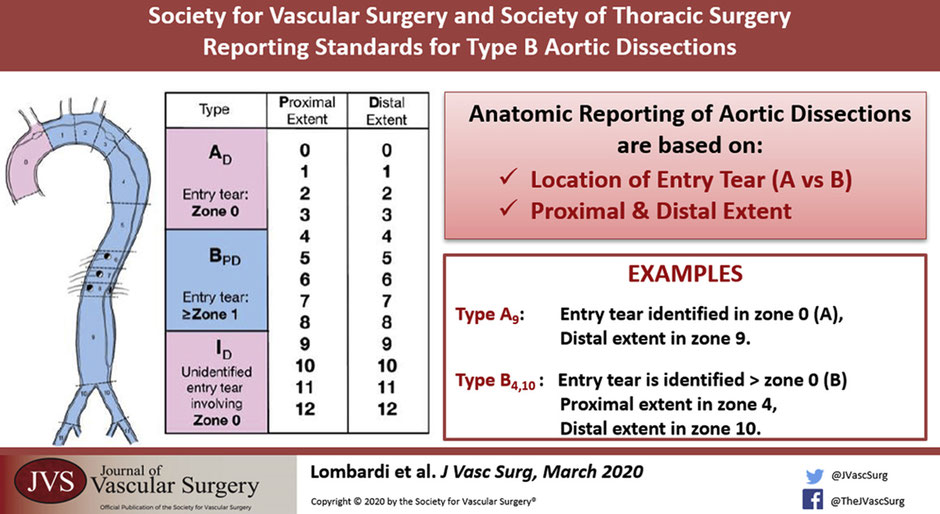
\includegraphics[width=13.06in]{images/thoracic_dissection1}

\begin{itemize}
\item
  Type A is now JUST the ascending aorta to the innominate, also
  called Zone 0.~
\item
  Type B is now~an entry tear in Zone 1 or greater~and distally to
  whichever zone the dissection lands in.
\end{itemize}

\textbf{This anatomical}~\textbf{classification~is based on reading the CT angio.
What else could we see on a CT angio that we have to know about?}

So aside from the aortic dissection its self, you could see a bleb of
contrast sticking out. That could be an penetrating aortic ulcer. That
is an atherosclerotic lesion that penetrates the internal elastic lamina
of the aortic wall.

Another key finding can be an intramural hematoma which is a hyperdense
crescent shaped hemorrhage within the aortic wall. There is no
identifiable direct communication between the true and false lumen. IMH
are classified in the same way but with the abbreviation IMH p-d zones.

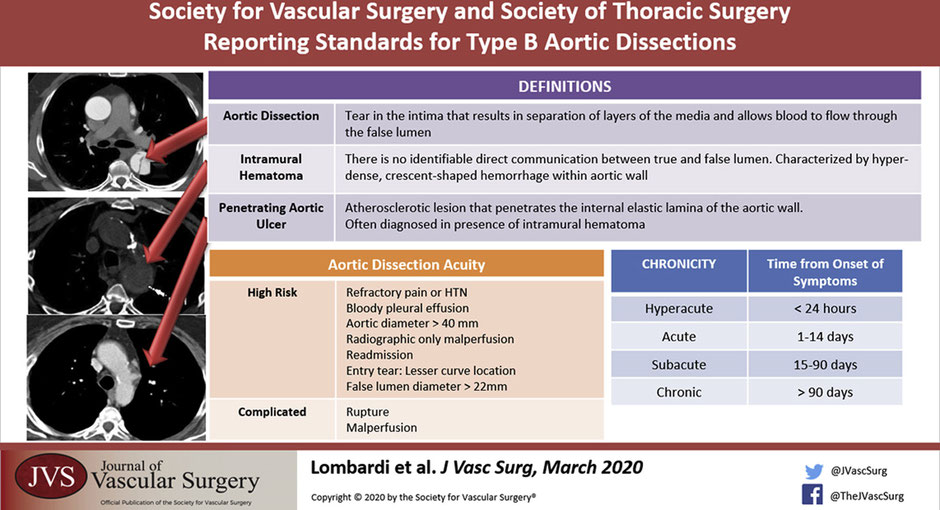
\includegraphics[width=13.06in]{images/thoracic_dissection2}

\textbf{Whats the significance of these two in combination?}

There is a higher chance of aortic rupture if a penetrating aortic ulcer
is seen with intramural hematoma.

\textbf{When a patient presents with an aortic dissection how can we classify
them clinically?}

\begin{itemize}
\item
  Uncomplicated~

  \begin{itemize}
  \item
    Stable hemodynamics~
  \item
    No evidence of malperfusion
  \item
    Pain controlled~
  \end{itemize}
\item
  Complicated~

  \begin{itemize}
  \item
    End organ ischemia / malperfusjon
  \item
    Rupture or impending rupture
  \end{itemize}
\item
  High risk~

  \begin{itemize}
  \item
    Uncontrollable pain / hypertension~
  \item
    Bloody pleural effusion
  \item
    Aortic diameter \textgreater40mm / False lumen diameter \textgreater{} 22mm
  \item
    Readmission
  \item
    Radiographic only malperfusion~
  \item
    Entry tear on the lesser curve
  \end{itemize}
\end{itemize}

\textbf{What is the danger of a false lumen? How does it lead to symptoms and
malperfusion? Likewise which arteries commonly branch off the true
lumen?}

The false lumen can lead to end organ ischemia as the intimal flap can
cover the ostia of branching vessels. This can be a static or a dynamic
obstruction.

Likewise it also leads to weakening in the wall of the aorta which can
become a threatened rupture or rupture if the diameter of the false
lumen is larger than 22mm.~

The celiac trunk, SMA, right renal typicaly come of the true lumen. Left
renal comes off the false.~

Also the dissection most commonly goes down into the left common illiac
rather than the right. You might be able to detect down stream effects
of this on clinical exam with reduced left sided groin pulse.

\textbf{What kind of patients get aortic dissections?}

Hypertension (older patients) / cocaine or Meth (younger patients)~

Marfans, loeys-Dietz, Ehlers danlos Type 4, Turners, Arteritis, Bicuspid
aortic valve.

We also have a traumatic cause of aortic dissections. That being called
blunt thoracic aortic injury:

\begin{itemize}
\item
  Grade 1: intima tear
\item
  Grade 2: IMH
\item
  Grade 3: Pseudo aneurysm
\item
  Grade 4: Aortic rupture.
\end{itemize}

\textbf{How do these patients present?}

Signs and symptoms --~Chest pain 90\% tearing pain radiating between the
shoulder blades.~

Chest pain extending to the abdomen abdomen? Think mesenteric ischemia
or aortic tear

Type A - Stroke 5-10\%,~Syncope 15\%, tamponade, carotid dissection,
paralysis.~

Others: MI -- Hypovolemic shock -- leg ischemia

\textbf{What is the~workup?}

Physical Exam --~Asymmetric pulses / blood pressure differences /
Diastolic murmur,

Investigations - CXR, EKG, D-dimer + Troponin, CTA, ECHO for type A.~

The big distinction is to find out if this is a type A or type B because
the treatment strategy is completely different.

\begin{itemize}
\item
  Type A need an emergent operation
\item
  Type B starts with medical management, follow up~CT angio~ +/- Trans
  esophageal echo in the OR. Reevaluate at 24 hours.~
\end{itemize}

\textbf{What are the details of Type A treatment?}

Operative treatment. 30\% op mortality. Cardiothoracics take the lead on
this one. However vascular surgeons should be involved in the management
of type A as after the repair, a type A can become a functional type B.

Type B is in the realm of vascular surgery. What is the first management
step after we have diagnosed a type B dissection?

Invasive impulse therapy. That means redusing the force of transmitted
impulse down the aorta. Blood pressure goals of 100-120mmHg. Hr \textless{}
60bpm.~

\textbf{How would you achieve that?}~

Start with a beta-blocker (esmolol or labetalol) first then a
vasodilator (nitroprusside). This is to stop the sympathetic surge after
vasodialation that could increase pressure and thus tearing forces
inside the aorta worsening the dissection.~

Initial CT, 72 hours, 3 months x 4, q6 months x2, q12 month. (Descending
thoracic aorta that dialates first.)~

\textbf{Why isnt open surgery indicated for type B dissections?}

Open surgery is not recommended due to the high mortality 30\% if \textless{} 48
hours. 18\% if \textgreater{} 49 hours.~

In the acute setting mortality can be up to 50\% with a 20\% paraplegia
risk. Its been described as sowing tissue paper.

\textbf{What is the management plan for a complicated Type B aortic
dissection?}

Start with invasive medical management and plan for TEVAR.~The goal with
TEVAR being to direct the blood flow into the true lumen and seal the
entry tear.~ If there was a dynamic obstruction (flap occludes branching
vessels.) Then TEVAR would reestablish the true lumen hence removing the
dynamic obstruction. Endovascular fenestration can also equalise the
pressure in the true and false lumen. \citep{lombardiSTABLEIIClinical2020}

For a static occlusion there could be a thrombus or stenosis in the
branched vessel so a stent might be indicated.~

\textbf{What are the major risks of TEVAR in the management of Type B aortic
dissections?}

Retrograde type A (reported 2\% in literature however it can be around
20\% in some experiences), 5\% paraplegia, and stent induced new entry.

\textbf{Is there a role for TEVAR in uncomplicated type B dissections?}

The INSTEAD and INSTEAD XL trials looked at uncomplicated Type B
dissections. There was NO statistical difference at 2 years comparing
OMT vs TEVAR but at 5 years there was good aortic remodelling and better
long term survival in patients treated in the subacute stage.~

Timing for TEVAR is a difficult choice. In chronic dissections the
septum thickens leading to a potentially difficult TEVAR. ~Anecdotally
TEVAR is best at 2w-3m.

\hypertarget{thoracoabdominal-aneurysms-taaa}{%
\section{Thoracoabdominal Aneurysms (TAAA)}\label{thoracoabdominal-aneurysms-taaa}}

02 Dec 2021: Mr.~Mohamed Barkat, Mr.~Nick Greaves, and Mr.~Michael
Jenkins

Resources

\begin{itemize}
\item
  \href{https://pubmed.ncbi.nlm.nih.gov/3951025/}{Crawford
  Classification}
\item
  \href{https://www.esvs.org/wp-content/uploads/2015/12/Consensus-document-ESVS-EATCS-Aortic-Arch.pdf}{ESVS recommendation of management of Thoracic aortic
  pathologies}
\item
  \href{https://www.optechtcs.com/article/S1522-2942(18)30073-4/fulltext}{Open Repair of Thoracoabdominal Aortic Aneurysm:
  Step-by-Step}
\item
  \href{https://www.circulationfoundation.org.uk/}{\textless https://www.circulationfoundation.org.uk\textgreater{}}
\item
  \href{https://www.bset.co.uk/}{\textless https://www.bset.co.uk/\textgreater{}}
\item
  \href{https://www.vascularsociety.org.uk/}{\textless https://www.vascularsociety.org.uk/\textgreater{}}
\end{itemize}

\textbf{Barkat:} {[}00:00:00{]} Welcome to another ruler club podcast in
association with audible bleeding. Today's guest is Mr.~Michael Jenkins,
a consultant Pasco surgeon, a summit, his hospital in Peter college,
healthcare NHS trust in London, Mr.~Jenkins, Trent at the Middlesex
hospital, London and a qualified in 1989. He trained in surgery at
Charing cross university college.

The Royal prompting, the Royal free hospital and was awarded the gold
medal at the FRCs exam. He was appointed as a Bhaskar consultant to
submit his and Chelsea and Westminster hospital in 2001, he was the
director of AAA screening in north west London from {[}00:01:00{]} 2011,
till 2018. He is currently the president of the vascular society of
great Britain and Ireland.

And he was chair of the circulation foundation between 2016 and 18. he
was the past president of the British society of endovascular therapy.
he was the director of the major trauma center as submit his hospital
between 2010 and 2016. He developed both a local and national tertiary
referral practice for thoracoabdominal Arctic aneurism and died.

My name is Hamad Barkat. I am a BASCA surgical trainee currently working
at Manchester of center. I am the Bosco society. I feel yet
representative of the rule of club.

\textbf{Greaves:} And my name is Nick grieves. I'm a year two consultants at
Manchester Royal infirmary, and I've got a specialist interest in open
aortic aneurysm repair. So this is particularly pertinent for me.
\textasciitilde\textasciitilde Um, \textasciitilde\textasciitilde thank you for joining us on this podcast, Mr.~Jenkins, a
very kind of you to share your time with this.

Good evening. During this episode, we hope to discuss the {[}00:02:00{]}
topic of thoracoabdominal aortic aneurysms with a view to providing
information that is relevant to those sitting, post-graduate exams, such
as the FRCs in the UK and V sites in the U S so we just want to break
this down into different areas, because it's a big topic.

firstly, just to kick us off a bit of sort of general background, you
tell us about your experience with thoracoabdominal aneurysms and how
you got into it? Any mentors you may have had.

\textbf{Jenkins:} So, as a trainee, I did do some work at the Brompton,\textasciitilde\textasciitilde{}
um,\textasciitilde\textasciitilde{} which was mainly tack. And I realized actually the majority of
cardiac surgeons, certainly in the UK are divided into coronary surgeons
and valve surgeons or thoracic, and very few. And she took on a Arctic
work.\textasciitilde\textasciitilde{} Um,\textasciitilde\textasciitilde{} during my training, then I was worked at all
three,\textasciitilde\textasciitilde{} uh,\textasciitilde\textasciitilde{} with George Hamilton and we did do some small cup
Donal aneurysms there.

And it was really only when I got appointed,\textasciitilde\textasciitilde{} um,\textasciitilde\textasciitilde{} I went to
Mary's because of the referral practice to Mary's and my interest and
{[}00:03:00{]} John Wolf was an established consultant there.\textasciitilde\textasciitilde{} Um,\textasciitilde\textasciitilde{}
and through referrals coming to the hospital, I just got involved and
took more and more along. And I think it's,\textasciitilde\textasciitilde{} um, you know,\textasciitilde\textasciitilde{} part
of your referral practice comes from people.

If you send the patients back alive, they send you more. So it's paying
attention to details, try and give a good outcome for

patients. And then I did go out to

Houston to, Visit has him Saffy for awhile. And has he is that Diane of
folk abdominal aneurysms. And it was very interesting and enlightening
to see how the system worked at Houston.

And we bought back some of those,\textasciitilde\textasciitilde{} um,\textasciitilde\textasciitilde{} skills and methods back to
Mary's after going out with one of our needs tests and you can't
underestimate the importance of a specialist in these statistics with
this work, which I'm sure we'll get to

later.

\textbf{Greaves:} Sydney.

\textbf{Barkat:} Mr.~Drinkers, let's start with some of the basics. Can you
take us through the Crawford classification {[}00:04:00{]} of truck off?
Don't overthink.

\textbf{Jenkins:} Yeah, so the COVID classification is relatively recent, to
be honest it was 1986. And I think it was really important because it's
very practical,\textasciitilde\textasciitilde{} um,\textasciitilde\textasciitilde{} classification really, depending on,\textasciitilde\textasciitilde{}
uh,\textasciitilde\textasciitilde{} cavity and how to get to an aneurysm.\textasciitilde\textasciitilde{} Um,\textasciitilde\textasciitilde{} it's a bit old
in terms of a terminology because they don't really follow a pattern\textasciitilde\textasciitilde{}
of, uh,\textasciitilde\textasciitilde{} one would expect\textasciitilde\textasciitilde{} sort of\textasciitilde\textasciitilde{} going one to four would be
getting either more extensive or less extensive.

And it's not quite like that. So type one is from the left subclavian
down to just below the diaphragm. And that's crucial because that
distinguishes it from a thoracic aneurysm, which you can get to just
from the chest and from a practical surgical approach. That's a very
important differentiating marker, but you have to go into a second
cavity,\textasciitilde\textasciitilde{} um,\textasciitilde\textasciitilde{} type two is the biggie.

So this is from the left sub clave all the way down to your tic
{[}00:05:00{]} bifurcation. So both dominal and so ACIC exposure, all the
visceral and Whelan, all trees and a lot of intercostal and numbers. So
big impact for cord supply, et cetera. So three is for mid chest down to
and involving the viscera renals and Dante or bifurcation.

And that's the one, which really is I suppose, the differentiator
between whether you go\textasciitilde\textasciitilde{} for,\textasciitilde\textasciitilde{} for the full support that's needed
in a type two, or whether you can whisk a clamp and go approach.\textasciitilde\textasciitilde{}
Um,\textasciitilde\textasciitilde{} and type four is characterized by being in most patients
accessible from the abdomen. I say in most patients, because there are
some anatomical, uh, situations with body habitus, which means that
going into the left chest is useful even for type four aneurism and then
type five. It w it was an additional classification that came in later,
which is a bit like a type three at the {[}00:06:00{]} top of the type one
at the bottom effectively.\textasciitilde\textasciitilde{} Um,\textasciitilde\textasciitilde{} but not everyone uses that.

\textbf{Greaves:} Okay. there appears to have been an increase in the
incidence of thoracoabdominal aneurysms. I mean, do you think it's a
true increase or does this relate to having scans for other reasons
picked up by accident and then going on from that? Just sort of many
referrals do you get in a year and what's your turn down?

Right? How many numbers are you actually doing in your practice year on
year?

\textbf{Jenkins:} So that's interesting because,\textasciitilde\textasciitilde{} um,\textasciitilde\textasciitilde{} the overall
instance of infrarenal atherosclerotic squat, again, isms is going down
and pre COVID every year in the national vascular registry, there was a
slight reduction in numbers. And I suppose that is a legacy of the end
of smoking for a big group of patients.\textasciitilde\textasciitilde{} Um,\textasciitilde\textasciitilde{} I think folk
abdominals are going up partly because we all now imaging more and more
people. and therefore we are imaging the chest and seeing them, which
perhaps wasn't the case. previously. So that's an {[}00:07:00{]} artificial
increase in instance, but also the weight of aortic dissection is on the
why's. So chronic,\textasciitilde\textasciitilde{} uh,\textasciitilde\textasciitilde{} post dissection aneurysms are

increasing.\textasciitilde\textasciitilde{} Um,\textasciitilde\textasciitilde{} and I think it's a small group, but there is
more knowledge about connective tissue disease and genetic studies and
family screening.\textasciitilde\textasciitilde{} Um,\textasciitilde\textasciitilde{} and that perhaps is also a small part of
Andover or increase. So over the next,\textasciitilde\textasciitilde{} you know,\textasciitilde\textasciitilde{} 10, 20 years,
certainly aneurysms are not going to go away.\textasciitilde\textasciitilde{} Um,\textasciitilde\textasciitilde{} and that group
of patients that have been affected are still around and there is a huge
number now within the NASP screening program under surveillance,\textasciitilde\textasciitilde{}
um,\textasciitilde\textasciitilde{} for small animism.

So it will come to fruition.

\textbf{Barkat:} you've just touched on a bit of difference in the geology
between thoracoabdominal aneurysms and abdominal aortic aneurysm.

So is there's a huge difference in the ecology between these two type of
aneurysm from your extreme.

\textbf{Jenkins:} \textasciitilde\textasciitilde Um, \sout{I don't think it's a huge difference. I think
{[}00:08:00{]} in terms of,} um,\textasciitilde\textasciitilde{} presentation,\textasciitilde\textasciitilde{} um,\textasciitilde\textasciitilde{} effectively,
the majority of aneurysms are asymptomatic. So they're found
incidentally. It is. rare that you get a symptomatic aneurysm? Yes. Some
can get tender as they perhaps approach a time when the wall perhaps is
going to breach pre rupture.\textasciitilde\textasciitilde{} Um,\textasciitilde\textasciitilde{} I think thoracoabdominal
aneurysms perhaps tend to be a bit more symptomatic and infrarenal. And
these are ones that perhaps affect go into the arch and past present
with hoarseness tension. Some of them can cause long kill
compression.\textasciitilde\textasciitilde{} Um,\textasciitilde\textasciitilde{} and there is a group that caused dark station
of the cross.

And it's,\textasciitilde\textasciitilde{} you know,\textasciitilde\textasciitilde{} you know, I've seen,\textasciitilde\textasciitilde{} uh,\textasciitilde\textasciitilde{} over the
years, the actual cross of a die from acts like an extrinsic lap and\textasciitilde\textasciitilde{}
it,\textasciitilde\textasciitilde{} it, can be extremely tight at that point. And there was a group
of patients that present with excruciating {[}00:09:00{]} pain, radiating
around their cost of margin. And this is tension on the cross and it's
often not thought of as a sign of a, of an aneurysm, but I think in that
group, it is, and the larger, the extent of aneurysm, I think. Things
like weight loss general,\textasciitilde\textasciitilde{} uh,\textasciitilde\textasciitilde{} poor health begins to become
increasingly seen in that group with chronic

aneurysms. So there are some subtle differences. The

The, other group that tends to occur, not in informing lack of isms is
the post dissection aneurysms, and the majority of those all known
about. But there was a time when type a dissections,\textasciitilde\textasciitilde{} um,\textasciitilde\textasciitilde{} as in
sort of DeBakey type one or a Stanford type one, which went all the way
down.

We're only monitored really with echo and the east ending. And the rest
was forgotten about, they got lost between two stools, between Claudia.
Fantastic. Follow-up that group,\textasciitilde\textasciitilde{} um,\textasciitilde\textasciitilde{} is a different group Cause
w we {[}00:10:00{]} already know they've got an aneurysm, so there are
subtle differences. And then the connective tissue group, I suppose, is
a bit different.

because they tend to have more extensive aneurysms rather than just
confined to the infrarenal sacrament, which is by far, in the way, the
most common for abdominal aneurysms.

\textbf{Greaves:} So you've mentioned quite a few different ideologies there.
And moving on to specifically thoracic aneurysms, know that as you said,
a quarter of these are associated with dissection in the past, as small
players will have underlying connective tissue disease, do you think
these patients will have a different threshold for intervention compared
to the non-connected tissue disorder?

\textbf{Jenkins:} Yeah, I think it's well established that,\textasciitilde\textasciitilde{} um,\textasciitilde\textasciitilde{} the
risk of rupture in any connective tissue disease. And I think we've
gotta be aware that the ones we talk about more family

states,\textasciitilde\textasciitilde{} uh,\textasciitilde\textasciitilde{} vascular stem loss. These are ones that are probably
the tip of the iceberg of a number {[}00:11:00{]} of other. Cases that we
don't know the genetic sequencing for, but behave differently. But data
from a I mentioned point of view is not quite as robust as one would
hope, but\textasciitilde\textasciitilde{} the\textasciitilde\textasciitilde{} threshold that most people would agree\textasciitilde\textasciitilde{}
for,\textasciitilde\textasciitilde{} for, non connective tissue disorders\textasciitilde\textasciitilde{} \sout{would be about six
centimeters. And that takes into account} the,\textasciitilde\textasciitilde{} the increased risks
of operating both in the chest and the Thor abdominal segment. I think
most people would agree that five centimeters is a better cutoff for
connective tissue patients. Some cardiac surgeons would do a young more
funny sending at four and a half centimeters. It does vary a little bit
geographically, a bit like the threshold for infer in Lanny wisdoms,
which varies from you have the states in UK. So you've got to look at
the patient in front of you and make a decision. and. I would certainly
upper {[}00:12:00{]} threshold for someone who was not so fit and perhaps
lower it a bit for a younger patient, and also be aware of it's
something all down atomically, a saccular bulge, something where you
think there could be a, my Kotick element.

Those are all very different to knee. You can't be reassured by a
dimension in an axial plane\textasciitilde\textasciitilde{} that\textasciitilde\textasciitilde{} that is safe. Savannah ups the
ante, in terms of,\textasciitilde\textasciitilde{} um,\textasciitilde\textasciitilde{} whether you would pair at an earlier
threshold and I'd include, they have a blowout for an eccentric Pau or
anything like that. It is not a conventional fusiform any wisdom.

\textbf{Barkat:} So Mr.

Dinkins, can you talk us through the issue zones of that water and why
do we need to know about these?

\textbf{Jenkins:} so is Mo was one of those useful classifications, you know,
there's lots of classifications in medicine,\textasciitilde\textasciitilde{} um,\textasciitilde\textasciitilde{} but it's nice
to find one that's actually got a use. And what this did is make sure
that everyone was on the same {[}00:13:00{]} page when you are
reporting,\textasciitilde\textasciitilde{} um,\textasciitilde\textasciitilde{} zones or seals zones for thoracic devices. So
that is important for two reasons.

One the extent of coverage and two, the complications increased, the
more proximally you go. And the main complication for that is stroke. So
issue Marla decided. to. Classifies zones. So zone zero, which is the
first most proximal zone is the sending a water up to and including the
brachiocephalic trunk, then between the brachiocephalic trunk and the
left common carotid artery is zone one between the left common carotid
artery and the left subclavian artery to zoom, to distill to the
subclavian artery then is zone three.

And in some people add in a sort of zone for distal to T4 level, which
is much lower down the thoracic air, water, and most thoracic stenting
will go really to zoom two or perhaps in,\textasciitilde\textasciitilde{} into, uh,\textasciitilde\textasciitilde{} into zone
three or {[}00:14:00{]} perhaps into zone two, The more proximal you go,
obviously yeah. more work needs to be done in terms of either extra
anatomical, deep bond Xing or using some form of fenestrated or launched
arch device with an increase in stroke

risk. But what this allowed people to do is compare different series. So
you're not just saying,\textasciitilde\textasciitilde{} well,\textasciitilde\textasciitilde{} these were a group of TIVA
patients. You could define exactly how

proximally they, they go. And the same, I I suppose, applies for the
corporate classification. It allows us,\textasciitilde\textasciitilde{} um,\textasciitilde\textasciitilde{} comparison within
thoracoabdominal groups.

And that's important with both survival and complication rates, because
if your series is mainly\textasciitilde\textasciitilde{} a\textasciitilde\textasciitilde{} type two or extend to dominoes,
you're going to have a very different outcomes from someone who's got
mainly type four. So of dominoes,\textasciitilde\textasciitilde{} um,\textasciitilde\textasciitilde{} and both glass patients
allow you to look at and {[}00:15:00{]} data between units.

\textbf{Greaves:} So if a patient has a thoracic aneurysm that affects their
ascending aorta, we obviously involve the cardiac surgeons. The patient
may require an elephant trunk procedure prior to intervention on the
descending aorta. Can you briefly summarize the difference between a
conventional elephant trunk and a frozen elephant trunk, and when to use
one over.

\textbf{Jenkins:} so,\textasciitilde\textasciitilde{} so, um, \sout{the vast majority of this I suppose, is
particularly pertinent to the section. So} \sout{we have to accept a little
of, is also more elective aneurysmal disease, but the main purpose}
in,\textasciitilde\textasciitilde{} in a type a or LT section is actually to protect the heart. So
people die of either for pericardium or stripping the colony osteo off
and getting ischemia.\textasciitilde\textasciitilde{} Um,\textasciitilde\textasciitilde{} the. purpose. All the time a repair is
to protect the heart. And to some extent for,\textasciitilde\textasciitilde{} uh, uh,\textasciitilde\textasciitilde{} uh, type
one, erotic, the is to then {[}00:16:00{]} ensure a true lumen flow
distally.\textasciitilde\textasciitilde{} Um,\textasciitilde\textasciitilde{} and so it was very popular because it was probably
the least invasive to do a short into position, a sending repair, but
that's really problems for later.

And as people became more adapt and better conjure protection and bring
protection\textasciitilde\textasciitilde{} um,\textasciitilde\textasciitilde{} it became more popular to do a more extensive
repair. The first sitting and this involves an

arch repair.\textasciitilde\textasciitilde{} Um,\textasciitilde\textasciitilde{} and then an acceptance that eventually the
descending thoracic aorta will still need to be repaired, but at a later
stage, Now you have to be aware that the ACE sending an arch is done
from a median sternotomy, and it's really difficult to get beyond the
left sub clave and form that,\textasciitilde\textasciitilde{} um,\textasciitilde\textasciitilde{} position.

So when the arch was done, it was felt that the elephant trunk came from
leaving,\textasciitilde\textasciitilde{} uh,\textasciitilde\textasciitilde{} an extra piece of {[}00:17:00{]} one within the
descending thoracic aorta in the two lumen of it during a section or in
the main lumen of a, of an aneurysm by a double sewing technique on the
distal and Estimote says and an inverting it, and it, would be left
free,\textasciitilde\textasciitilde{} um,\textasciitilde\textasciitilde{} perfused in the descending, thoracic aorta.

And the benefit of that was when one came back to then do the descending
thoracic segment,\textasciitilde\textasciitilde{} um,\textasciitilde\textasciitilde{} via left thoracotomy, You could very
quickly open the altar and clamp

that,\textasciitilde\textasciitilde{} um,\textasciitilde\textasciitilde{} deck on. And then you've got a ready, made an estimate
SIS to D to do your segment, which was much easier. And it meant you
didn't have to grow up and dissect to the left, to play in whether it be
scar tissue\textasciitilde\textasciitilde{} in a,\textasciitilde\textasciitilde{} in a, previous, in estimate basis. Now,
what\textasciitilde\textasciitilde{} um,\textasciitilde\textasciitilde{} realized is that they could help with this procedure by
actually facilitating a device which had four blond shares or three or
{[}00:18:00{]} four,\textasciitilde\textasciitilde{} um,\textasciitilde\textasciitilde{} bond shares on a piece of Dacron, which was
sized to be a, an arch replacement. And these were ready. So norm survey
took 10 millimeter bunches to allow an extra pipe for rewarming. And
these could then be sewn to be a nominate, carotid and subclavian and
attached to, and piece of Dacron was then a stint graft, which could
then be placed distally in, lieu of what was previously a floppy piece
of that cone.

And two manufacturers really geo-tech and two-way Alltech,\textasciitilde\textasciitilde{} uh,\textasciitilde\textasciitilde{}
have made these devices, which just facilitate and make things much easy
and so-called FET or frozen elephant trunk,\textasciitilde\textasciitilde{} um,\textasciitilde\textasciitilde{} has now become
quite popular. I don't quite know why it's called frozen, but I think it
perhaps means that the thoracic eight segment is,\textasciitilde\textasciitilde{} uh,\textasciitilde\textasciitilde{} is, stiff
as in a supported evolve rather than just a floppy deck on

segment.

\textbf{Barkat:} {[}00:19:00{]} So if we look at it at the isolated,\textasciitilde\textasciitilde{} uh,\textasciitilde\textasciitilde{}
thoracic aneurysm, Mr.~Jenkins, can you tell us briefly about the
principle of T VAR and what's the optimal landing zone and in your
opinion is rapid ventricular pacing required when deploying these
stents.

\textbf{Jenkins:} So I think the isolated, thoracic aneurysm is a perfect
treatment,\textasciitilde\textasciitilde{} um,\textasciitilde\textasciitilde{} for TIVA because\textasciitilde\textasciitilde{} \sout{it actually, it, it
fulfills all those minimally invasive credentials in that you can do, an
endoluminal approach. And if you can get a good seal zone, proximally
and distally,} it\textasciitilde\textasciitilde{} saves us a lot to me. And it's a massive
difference for the patients,\textasciitilde\textasciitilde{} you know,\textasciitilde\textasciitilde{} unfortunately I suppose
those cartoons you see on the industry and for it's so vanishingly rare
when you've got a perfect proximal and distal landing zone and have
really straight . um, I think for the majority of cases you still needed
to send to me to seal zone proximally and distally. And I think if
you've got a very {[}00:20:00{]} torturous aorta, you've got to think about
a longer, seal zone you want to land,\textasciitilde\textasciitilde{} um,\textasciitilde\textasciitilde{} in an area where there
is a good power level walled segment. And you've got to be careful of
so-called bird beaking when they, when a stiff, less conformable
device,\textasciitilde\textasciitilde{} um,\textasciitilde\textasciitilde{} lands perfectly on the outer curve, but holds off on
the inner curve.

So as you've got a lip, which protrudes and that's going, to allow blood
to get under that and cause sense, graph crushing, I think modern
devices have been now much more conformable. We've learned the lessons
of oversizing and the problems associated with oversizing. We've learned
how to tape a stent grafts when there's mismatch between proximal and
distal. and we've also got customed taper devices now. So these have all
significantly improved things, but there's still no getting away from
the fact that some anatomy is {[}00:21:00{]} not well adjusted to the
currently available stent, grafts

and Gothic arches, a particular problem.

I've already mentioned vape torturous and beta launch sacks, which allow
a stench graph to move away from the wasting line to the out to curve.

And as they affect sectors and shrink, you can imagine that draws on
both the proximal and distal seals zone and reduces them.\textasciitilde\textasciitilde{} So,
um,\textasciitilde\textasciitilde{} I think you can sometimes get away with a shorter lending zone.
If, for example, you're doing a post traumatic aneurysm where it's only
on one segment VNO the outer wall where there's a problem. Um, but for
the vast majority of two aneurysms, you need that seal zone and you do
need to oversize

to achieve that.\textasciitilde\textasciitilde{} Um,\textasciitilde\textasciitilde{} you can, of course go more proximately. And
I think the majority of aneurysms app left some in area, you can just
drop them {[}00:22:00{]} blood pressure to a systolic of 70 or 80
pharmacologically.

Once you go more proximal to that, especially if you've got a custom
device where with a scallop or bond device where you need an absolutely
critical lending zone,

you then really need to achieve a short transient period of circulatory
arrest either with the dentist's scene, which is perhaps sometimes a bit
unreliable. Or\textasciitilde\textasciitilde{} rapid ACEing\textasciitilde\textasciitilde{} rapid pacing does come with
complications though. And,\textasciitilde\textasciitilde{} you know,\textasciitilde\textasciitilde{} you

can get ventricular puncture from rapid pacing,\textasciitilde\textasciitilde{} um,\textasciitilde\textasciitilde{} and it can
be difficult. There are some newer techniques in terms of Keval,
occlusion, balloons as well, which basically stop venous blood returning
to the heart with a reduction in outputs. those are gaining popularity
certainly in Germany. And they can be quite effective for that.\textasciitilde\textasciitilde{}
Um,\textasciitilde\textasciitilde{} I think,\textasciitilde\textasciitilde{} you know,\textasciitilde\textasciitilde{} having. Tip capture on devices and
better, more accurate {[}00:23:00{]} deployment and better imaging does
allow you\textasciitilde\textasciitilde{} to,\textasciitilde\textasciitilde{} to, actually be more accurate in deployment, but
there are still problems.

These devices have been inserted to very torturous IDX systems
sometimes, and they retain some energy. And when you deliver them by
removing that sheath, sometimes that energy is still and they can jump
forward as well as back.\textasciitilde\textasciitilde{} Um,\textasciitilde\textasciitilde{} and that can cause problems because
you end up covering a vessel that you didn't intend to So you've just
explained in detail at T virus is a great option and a lot of cases, but
I presume you still believe there is a place for open repair in
isolated, thoracic aneurysms, and why.

Yeah, I'm not so sure in isolated, thoracic aneurysms, unless for some
reason that they're not suitable\textasciitilde\textasciitilde{} for\textasciitilde\textasciitilde{} for TIVA,\textasciitilde\textasciitilde{} um,\textasciitilde\textasciitilde{} I
think if you've got problems with,\textasciitilde\textasciitilde{} um,\textasciitilde\textasciitilde{} a mycotic aneurysm or a
fistula in for Blanca sore, Fergus, the, these are our big problems with
high mortality {[}00:24:00{]} and your duty bound to go.

And certainly with connective tissue

patients,\textasciitilde\textasciitilde{} um,\textasciitilde\textasciitilde{} again, open has advantages, but you all, and it is
possible sometimes to bridge between repairs. So I, I think in some of
the younger connective tissue patients, they will end up having certain
segments were paired at different stages of their life. And although
it's probably now accepted that all endovascular is not a good option
for these patients. If you've got. Dotcom proximally and deck on
distally already. Well then bridging those segments,\textasciitilde\textasciitilde{} whether\textasciitilde\textasciitilde{}
with a, an endovascular device actually works very well because although
the Dacron will slowly dilate it, won't out laters as much as, normally
all tick tissue. So there are options, but I think in reality, isolated,
thoracic aneurysms on Weasley where, and probably {[}00:25:00{]} VAR can

be used for the majority

of

them.

\textbf{Barkat:} So Mr.~Dink is

moving on to throw up domino aneurysm now. \sout{So} we earlier used the
Crawford classification to describe the anatomical extent of the
thoracoabdominal aneurysm. So let's talk firstly, about type 1, 2, 3,
and five, which involved the thoracic of water to a greater or lesser
extent as well as Daptone award.

And we'll come back to type four later on in this podcast. So type two
open throttle. Aneurysm is arguably the most invasive operation a
patient can undergo and carries 30 day mortality in excess of \sout{15 to 20
to} 10 to 15\%. What is the sash position for type two that you
currently use in your practice?

And is \textasciitilde\textasciitilde there \textasciitilde\textasciitilde there's any strong evidence?

\textbf{Jenkins:} \textasciitilde\textasciitilde So, \sout{as I suggested earlier,} the,\textasciitilde\textasciitilde{} the, evidence
is that it's a bit historical and most people would actually say about
six centimeters. I think that can be brought down a little bit for
connective tissue patients {[}00:26:00{]} and can go up a little bit for
atheroma to see patients. But in general, you're talking about a younger
segment You know, This is not an operation for people in their
eighties.\textasciitilde\textasciitilde{} Um,\textasciitilde\textasciitilde{} and they've got to be pretty physiologically in
really good shape\textasciitilde\textasciitilde{} to get\textasciitilde\textasciitilde{} to get to this because it is a. A big
onslaught physiologically on them and it's not just getting them off the
table.\textasciitilde\textasciitilde{} It's,\textasciitilde\textasciitilde{} It's, getting them then out of ITU and out of
hospital and to recover back to their baseline.

And I think that's one of the things that

can be really difficult. You are taking patients who are effectively
functioning quite well, and they're often rather to be asymptomatic and
you're putting them through a proof or lactic operation to\textasciitilde\textasciitilde{} try,\textasciitilde\textasciitilde{}
try and prevent something, which no one quite knows if will happen or
when it'll happen.

\textbf{Greaves:} So to that end, can you talk us through the decision making
process when you're assessing {[}00:27:00{]} a patient with a thoraco
abdominal aneurysm 1, 2, 3, or five.

\textbf{Jenkins:} Yeah. I think,\textasciitilde\textasciitilde{} you know,\textasciitilde\textasciitilde{} it is really,\textasciitilde\textasciitilde{} um,\textasciitilde\textasciitilde{}
Dependent on anatomy, physiology and the patient in front of you. And it
is this a bespoke assessment for an individual patient. So firstly, I
think you have got to look at what are the options for that patient. And
then it goes from conservative to endovascular, to open surgery.

And,\textasciitilde\textasciitilde{} you know,\textasciitilde\textasciitilde{} the endovascular domain has changed hugely now
with the availability of bondage devices. when I started there weren't
custom devices like that. Yes, fever was just coming out, but, and we
did use long covered stents going through devices with TIVA above.
But,\textasciitilde\textasciitilde{} um,\textasciitilde\textasciitilde{} there wasn't the

option\textasciitilde\textasciitilde{} for,\textasciitilde\textasciitilde{} for what we've now got from an endovascular
perspective. So I think you've got to choose the patients that. have
either. Unsuitable for endovascular, or {[}00:28:00{]} are we really going
to benefit from a doability of an open approach?

So those are the

two big differences,\textasciitilde\textasciitilde{} I suppose.\textasciitilde\textasciitilde{} And they all are because one
you're going for gold standard approach because you think they're life
expectancy warrants that the one is a bit hops in this because they
haven't got another endovascular option. And these range from people
with very tortuous anatomy to difficult renals with four perhaps
difficult renos, renal arteries, or early divisions or ones that aren't
suitable as target vessels,\textasciitilde\textasciitilde{} um,\textasciitilde\textasciitilde{} Y to, to sometimes complex
dissections, which. On suitable for an endovascular approach. So it is
very variable, but I suppose the first thing when you're considering it
is, is, the patient going to get through this and get out of hospital.
And that really is,\textasciitilde\textasciitilde{} uh,\textasciitilde\textasciitilde{} looking at them in the eye. What's their
quality of \textasciitilde\textasciitilde{} Like\textasciitilde\textasciitilde{} what's their family support,\textasciitilde\textasciitilde{} like,\textasciitilde\textasciitilde{} are

they

up for {[}00:29:00{]} this?\textasciitilde\textasciitilde{} Um,\textasciitilde\textasciitilde{} and the second one then is
anatomical difficulties. Is there a Shanghai auto? Is there a lot of our
bathroom, which is diseases? A lot of calcification of a target vessel
is difficult. Um, that sort of thing. And it comes down to them. It's
rare that there's a hundred percent or 0\% decision. It's building up
relative contraindications. And some of them are pretty simple, like
access problems for endovascular. And\textasciitilde\textasciitilde{} it's,\textasciitilde\textasciitilde{} it's, a combination
of those which then will sway you in one way or the other. And if
anything, that decision-making is probably more pertinent for type three
and type four, where there really is a different option. And these
patients are perhaps in their sixties and seventies with classic Latham,
which is disease. The really young fit non connective tissue patient
with a type two is aware beast.

\textbf{Barkat:} So Mr.~Has {[}00:30:00{]} some textbook specifically for
connective tissue disease. We'll always prefer an open approach for them
rather than in the vascular approach.

Do you still agree with this.

\textbf{Jenkins:} Yeah, I do.\textasciitilde\textasciitilde{} Um,\textasciitilde\textasciitilde{} I think certainly,\textasciitilde\textasciitilde{} um,\textasciitilde\textasciitilde{} what
were you know about,\textasciitilde\textasciitilde{} um,\textasciitilde\textasciitilde{} patients who've had endovascular,\textasciitilde\textasciitilde{} I
mean,\textasciitilde\textasciitilde{} total endovascular approaches connective tissue diseases. They
don't last.\textasciitilde\textasciitilde{} so, uh,\textasciitilde\textasciitilde{} they may last five years or and then get
progressive,\textasciitilde\textasciitilde{} uh,\textasciitilde\textasciitilde{} aortic dilatation and,\textasciitilde\textasciitilde{} um,\textasciitilde\textasciitilde{} loss of
those seals zones,\textasciitilde\textasciitilde{} uh,\textasciitilde\textasciitilde{} whether that is the natural history of
the native disease or whether it is regional force hooks, bobs, whatever
the device is unclear.

But when you, so these pensions and just touching the back end of a
needle on the anterior wall will create a massive problem or just being
a little bit clumsy and you get a regional town. It's very clear that a
stiff device sitting in those for many years were with 60 beats, 70
beats per minute, {[}00:31:00{]} going through it and often

hypertension isn't going last.

So I think we now know that, but there are some caveats, as I mentioned
earlier, bridging between previous prosthetic open repairs is a
possibility and sometimes lifesaving situation. When someone is
presented with a rupture, you may have to use an endovascular
approach,\textasciitilde\textasciitilde{} um,\textasciitilde\textasciitilde{} and that's reasonable.\textasciitilde\textasciitilde{} Um,\textasciitilde\textasciitilde{} but sometimes
be prepared then to treat that as a bridge and go back to do a
definitive repair when have calmed down and in the cold light of day.

\textbf{Greaves:} So we don't really have the scope to dive into complex
endovascular repair in this episode, but can you describe sort of the
broad principles of your operative approach to open thoracoabdominal
aneurysm repair, type two, because it's the most extensive.

\textbf{Jenkins:} Yeah. \sout{So, um,} in general, in terms of the patient,\textasciitilde\textasciitilde{}
um,\textasciitilde\textasciitilde{} for anything juxta renal or type four, I tend to have a patient
supine on the {[}00:32:00{]} back, but with a break in the table at the
level of the, between the costal margin and the anterior superior iliac
spine, and by breaking the table at that level, you can massively
increase the,\textasciitilde\textasciitilde{} um,\textasciitilde\textasciitilde{} exposure to that segment.

As I suggested earlier,\textasciitilde\textasciitilde{} um,\textasciitilde\textasciitilde{} there are some patients even with a
type four approach. that. Demand a thoracoabdominal and this is a left
dog, abdominal, and for a type four, if you're doing a left sock
abdominal, it's usually for someone with a very narrow costal margin,
have a cute angle on that. Sometimes a more petite frame female
patient,\textasciitilde\textasciitilde{} um,\textasciitilde\textasciitilde{} or sometimes a patient that\textasciitilde\textasciitilde{} has, um,\textasciitilde\textasciitilde{}

\sout{the,} the class is very high on the aorta.

And if you look at CT scans is something I've realized over many years
that not everyone is the same. So where the celiac Lancaster male can be
in a different proportion, depending on\textasciitilde\textasciitilde{} their,\textasciitilde\textasciitilde{} where the cost of
marching and the skeleton is, {[}00:33:00{]} which can make them easier or
hard\textasciitilde\textasciitilde{} to,\textasciitilde\textasciitilde{} to. get to. And certainly in a situation, if there is a
rupture within the left side of the abdomen, you wouldn't really want to
go into that without getting proximal control, because as you do the
visual rotation, you, you could have catastrophic bleeding.

So under those circumstances, I'd also go into the left chest with a
reasonably low segment so that you've got it. You can place a clamp
ready before doing the vessel

rotation. So for type four the one above then the higher you go, the
higher or thoracotomy and the more,\textasciitilde\textasciitilde{} um,\textasciitilde\textasciitilde{} tipped over you need the
patient. So for a type two, you're going probably fifth space and the
shoulders are at 90 degrees and the pelvis is 60 degrees for type three.
You're slightly further over. So you're down to about 60 degrees and
you're perhaps in the seventh intercostal space. So the more and the
lower you go, then light up to {[}00:34:00{]} being pretty much suited. The
left arm is put over

top. You mark

the scapular,\textasciitilde\textasciitilde{} um,\textasciitilde\textasciitilde{} and \sout{you, you go into,} you go into the
chest and abdomen. I tend to go into parents and early into the abdomen,
so I can see the bowel of all people who do a retroperitoneal

approach.\textasciitilde\textasciitilde{} Um,\textasciitilde\textasciitilde{} I tend to divide the diaphragm down to the central
ligament and mark that.\textasciitilde\textasciitilde{} Um,\textasciitilde\textasciitilde{} and then effectively you are looking
at\textasciitilde\textasciitilde{} \sout{your clamp soon. So your dissect around your, your Klemp
zone,} um,\textasciitilde\textasciitilde{} both proximally and distally.\textasciitilde\textasciitilde{} Um,\textasciitilde\textasciitilde{} we don't tend
to expose the celiac and SMA in between kill all the white renal. The
left renal It's important\textasciitilde\textasciitilde{} to find,\textasciitilde\textasciitilde{} to find the left artery.\textasciitilde\textasciitilde{}
Um,\textasciitilde\textasciitilde{} visceral rotation is effectively you. Extend the left colon up,
find the white line and get under that and get blight on just so our
secures to get right down on so as early on, and then it is a relatively
bloodless field. Everything is taken {[}00:35:00{]} me to leave The, you
were to answer the way I always take for left kidney up. You will see in
the textbooks and some of your bland advocate,\textasciitilde\textasciitilde{} um,\textasciitilde\textasciitilde{} keeping the
left kidney down.\textasciitilde\textasciitilde{} Uh,\textasciitilde\textasciitilde{} I that's up to madness to be honest.\textasciitilde\textasciitilde{}
Um,\textasciitilde\textasciitilde{} I can't see any point in it, so everything rotates up then out
for way. And it it looks a bit strange. It looks a bit like a
post-mortem it looks very odd to see the whole left side of cavity with
all you've got is diaphragm muscle, so ass and nothing else left.\textasciitilde\textasciitilde{}
Um,\textasciitilde\textasciitilde{} it does give you a very safe exposure then\textasciitilde\textasciitilde{} to,\textasciitilde\textasciitilde{} to, Vail.
to. I don't tend to go round with slings.\textasciitilde\textasciitilde{} Um,\textasciitilde\textasciitilde{} Avandale, which I
think that can cause problems, uh, tend to go around,\textasciitilde\textasciitilde{} um,\textasciitilde\textasciitilde{} with
my fingers and be very aware of,\textasciitilde\textasciitilde{} uh,\textasciitilde\textasciitilde{} the light sided lumbers or
intercostals because you really don't

want to cause a problem there because you easily get into the white
chest from exposure.

So you have to be a bit careful as soon as you can see exactly\textasciitilde\textasciitilde{}
where,\textasciitilde\textasciitilde{} where, you're

getting round {[}00:36:00{]}

\textbf{Barkat:} So in specifically in type two,\textasciitilde\textasciitilde{} uh, uh, \textasciitilde\textasciitilde people, a
lot of people establish a left heart bypass. Do you always operate in
that way? And do you use a cardiac surgeon and the setting, or how do
you approach type two in terms to reduce the pressure in the left heart

\textbf{Jenkins:} \sout{So, um,} I think type two, now you are mandated to have
some sort of. Adjunct to keep the rest of the body perfused while you're
doing the proximal anastomosis. I think in an elective setting,\textasciitilde\textasciitilde{}
um,\textasciitilde\textasciitilde{} left heart bypass is the mind's way forward,\textasciitilde\textasciitilde{} um,\textasciitilde\textasciitilde{} because
it does give you more flexibility and it allows you then to sequentially
clamp and keep the legs, the vessel or the kidneys perfused. There are
some negative aspects to laptop bypass though, in terms of needing a
much higher ECT and bleeding is the enemy here. So the more you
anti-coagulate, the more problems you've got, it's also not pulsatile
flow.\textasciitilde\textasciitilde{} Um,\textasciitilde\textasciitilde{} and you're putting all your, your, cells {[}00:37:00{]}
through a pump.\textasciitilde\textasciitilde{} Um,\textasciitilde\textasciitilde{} and you've got to be aware of it, increased
problems around stroke and everything else that goes with that. I think
it's,\textasciitilde\textasciitilde{} um,\textasciitilde\textasciitilde{} It is very convenient for that set up because you can
get to in for your problem, move in quite easily.\textasciitilde\textasciitilde{} Um,\textasciitilde\textasciitilde{} femoral
cannulation is quite easy for you to return.

like,\textasciitilde\textasciitilde{} Um,\textasciitilde\textasciitilde{} and then you've got the option then of individually
calculating,\textasciitilde\textasciitilde{} uh,\textasciitilde\textasciitilde{} celiac SME,\textasciitilde\textasciitilde{} uh,\textasciitilde\textasciitilde{} for perfusion. Usually
wrinkles are cooled down.

If you've got a perfusionist as well, you can get cold, profuse for the
renals. So it gives you more flexibility. And if things go wrong, you've
then got an option to switch to,\textasciitilde\textasciitilde{} um,\textasciitilde\textasciitilde{} conventional bypass if
needed or eval drain out and go to circulate Triovest and cool-down
things go very wrong. So it does give you. you. More options, however,
in a more emergency setting and approach, should I really like and tends
to work quite well for us is to do what I {[}00:38:00{]} call an ax fem
approach. So you would\textasciitilde\textasciitilde{} put, uh,\textasciitilde\textasciitilde{} use an XM graft onto the light
subclavian lots, obviously tunneled outside of a body onto the white
wall and use the other limb.

Then\textasciitilde\textasciitilde{} as,\textasciitilde\textasciitilde{} as, a single cannular, usually for estimate, cause SMA
is the king vessel with all of us. Most of the other things can go. If
you lose the SMA, you've got a dead patient. And that allows you to do
perhaps an emergency procedure, perhaps a amid type three approach
without some of the problems associated with left heart bypass. It
allows you to have a lower act. It gives you pulse style flow. You're
not smashing all your cells up all the time. It's relatively quick and
straightforward to do.\textasciitilde\textasciitilde{} Um,\textasciitilde\textasciitilde{} you don't have to move. Ally's a
perfusionist and everything else that goes with that.\textasciitilde\textasciitilde{} Um,\textasciitilde\textasciitilde{} and
it's worked well for us in emergency settings.\textasciitilde\textasciitilde{} Um,\textasciitilde\textasciitilde{} and it's
better than a clamp and go approach because with a clamp and go
approach, the type of three you need sort of {[}00:39:00{]} in 15 minutes
for you, inlay and estimates of the top, the clock is already on. If you
get down to the visceral segment and

it's not looking very attractive, and you've got to do some removal of
formless and a bit of what I call gardening to get your Corolla patch on
them.

And if you've got to reimplant the left kidney separately,\textasciitilde\textasciitilde{} it's,\textasciitilde\textasciitilde{}
it's a old time pressure and there's no for something to wrong
there.\textasciitilde\textasciitilde{} Um,\textasciitilde\textasciitilde{} and that's where this gives you a bit more breathing
space that you've got the lower body profused while you're doing your
POCs on an estimate basis.

\textbf{Greaves:} So, as you've mentioned, open repair is clearly a high
tariff, high risk operation apart from death. Are there any specific
complications to the open approach?

\textbf{Jenkins:} Yeah, I think,\textasciitilde\textasciitilde{} um,\textasciitilde\textasciitilde{} yeah,\textasciitilde\textasciitilde{} the, the,\textasciitilde\textasciitilde{} the big
problem is bleeding.\textasciitilde\textasciitilde{} So, you know,\textasciitilde\textasciitilde{} bleeding is and clamp times,
those are the things that, that,\textasciitilde\textasciitilde{} um,\textasciitilde\textasciitilde{} cause problems for those
patients who survive. So problems with launch transfusion,\textasciitilde\textasciitilde{} um,\textasciitilde\textasciitilde{}
and cause problems with {[}00:40:00{]} then ventilation afterwards.\textasciitilde\textasciitilde{}
Um,\textasciitilde\textasciitilde{} renal ischemia,\textasciitilde\textasciitilde{} um,\textasciitilde\textasciitilde{} is an issue of people will quote a
40 to 50 minutes,\textasciitilde\textasciitilde{} um,\textasciitilde\textasciitilde{} enlist schemic time, a warm ischemic time.
You can actually get away for longer than that. The kidney probably
some. Extra blood supply, but it, once beyond that, you are then getting
increasing problems\textasciitilde\textasciitilde{} with,\textasciitilde\textasciitilde{} with likely failure. Now, yes, they
may need a bit of, to go on the hemofilter for temporary support.\textasciitilde\textasciitilde{}
Um,\textasciitilde\textasciitilde{} but a lot of these patients who already lost a lot of nephrons,
so they, haven't got a huge amount of capacity to lose more. And that's
the problem. And that's why EGF or high creatinine is a really important
prognostic marker of outcome in this patients. I think\textasciitilde\textasciitilde{} it's,
\textasciitilde\textasciitilde it's

like a bolometer\textasciitilde\textasciitilde{} on their,\textasciitilde\textasciitilde{} on their, microcirculation. the big
one, of course, the Achilles heel of these approaches, whether it's end
all work from is called {[}00:41:00{]} ischemia.\textasciitilde\textasciitilde{} Uh,\textasciitilde\textasciitilde{} and that is
because the segment of blood supply to the cord comes from all the
intercostals and lumbers. and if you've got that aneurysm extending both
proximally and distally involving the internal ex and the left, some
clave in you're taking out

your crucial collateral supply, which helps with

cord supply as well. And that is why trying to,\textasciitilde\textasciitilde{} \textasciitilde\textasciitilde{} Maintain a
blood supply,\textasciitilde\textasciitilde{} um,\textasciitilde\textasciitilde{} and getting, for example, getting the lengths
back in circuit early, whether that's,\textasciitilde\textasciitilde{} um,\textasciitilde\textasciitilde{} with large sheets,
during a long blanched approach or, and we're moving machines or getting
the leg supply earlier in an open approach,\textasciitilde\textasciitilde{} um,\textasciitilde\textasciitilde{} and keeping the
lefts of caving in circuit, these are all other important things and
having paying attention to the mean arterial pressure in theater have a
spinal dreams working.

All of that is crucial in terms of trying to protect the cord

as much as

{[}00:42:00{]} possible.

\textbf{Barkat:} So the major issue is the spinal cord ischemia, and we
mentioned briefly the plot supply of the spinal cord for the sake of the
exam. Can you just \textasciitilde\textasciitilde recap, \textasciitilde\textasciitilde recap for us the blood supply of the
spinal cord for the audience who's going for the.

\textbf{Jenkins:} So

\textbf{Barkat:} exam

\textbf{Jenkins:} it's complicated actually. Yeah. Yes, sir. and posterior
spinal arteries. But I think depending on what level you are in the
court, they get a blood supplier from a more dominant,\textasciitilde\textasciitilde{} um,\textasciitilde\textasciitilde{}
approach. So higher up in the cord, survival, higher thoracic vertebral
arteries are important to there. so hence the importance of a left to
play in the lower you go there and they can have to become a bit less
important.

And the actual segmental arteries intercostals,\textasciitilde\textasciitilde{} uh,\textasciitilde\textasciitilde{} become
dominant much as it's talked about the archery of a dam. Kovich I
think,\textasciitilde\textasciitilde{} you know,\textasciitilde\textasciitilde{} yes, there may be a dominant vessel at about
that level, but it's. It's rarely

one, absolutely single {[}00:43:00{]} one. That if you think that you've got
that the rest and matter, I think they all matter.

And then the more distally you go launches coming in collateral supply
from internal lilacs meeting say cool, all those contribute to a
collateral circulation that should be seen in some ways, all connected.
And that is why,\textasciitilde\textasciitilde{} um,\textasciitilde\textasciitilde{} more recently in endovascular,\textasciitilde\textasciitilde{} uh,\textasciitilde\textasciitilde{}
purchase staging repair is really useful because you can not allow the
surviving arteries then to remodel and increase flow.

And it's why doing a type two repair. When you get the whole lay auto,
it's very important. to.

Block the intercostals early either by sewing them off or putting big 10
for a little Pruitt ballooning,\textasciitilde\textasciitilde{} um,\textasciitilde\textasciitilde{} to stop you,\textasciitilde\textasciitilde{} uh,\textasciitilde\textasciitilde{}
losing blood from that collateral,\textasciitilde\textasciitilde{} uh,\textasciitilde\textasciitilde{} supply. And it keeps the
pressure in, in, in the spinal cord.\textasciitilde\textasciitilde{} Um,\textasciitilde\textasciitilde{} and that's why, of
course the {[}00:44:00{]} differential position of that blood supply is why
patients then get a particular form of problem with,\textasciitilde\textasciitilde{} um,\textasciitilde\textasciitilde{}
motor,\textasciitilde\textasciitilde{} um,\textasciitilde\textasciitilde{} problems and sometimes preservation of sensation

\textbf{Greaves:} So purely for exam purposes and a bit of physiology. Can
you remind us how to calculate the spinal cord profusion?

\textbf{Jenkins:} all that is really is map minus the CSF pressure. So it's
your mean arterial pressure Take out the CSF pressure and that's what
you've got perfusing it. And that really is a useful equation to
remember because it actually,\textasciitilde\textasciitilde{} uh,\textasciitilde\textasciitilde{} allows you to decide what's
the way to enhance that as much as possible.

And that of course is to increase

map,\textasciitilde\textasciitilde{} um,\textasciitilde\textasciitilde{} and decrease your CSF pressure. And we do that by
enhancing the mean arterial as much as

possible, and actually draining off CSF with a spinal drain to reduce
your CSF pressure, to allow more blood {[}00:45:00{]} into\textasciitilde\textasciitilde{} the\textasciitilde\textasciitilde{} the
cord. I think people perhaps get a bit hung up on,\textasciitilde\textasciitilde{} um,\textasciitilde\textasciitilde{} spinal
yeah.

Image and it's important.

It is just as important to maintain oxygenation and hemoglobin over
hundreds and reduce blood loss. And. all those. Other things are as
crucial.\textasciitilde\textasciitilde{} Um,\textasciitilde\textasciitilde{} and it's an adjunct. It's not, it shouldn't be seen
in isolation. It's one of many adjuncts to try and help

with that.

\textbf{Barkat:} So if you're looking at the mechanism of the spinal cord
ischemia on the open throw cop dollar award, the Kennedys and repair, do
you think it's related the blood loss or a clamp or implantation of the
intercostal?

\textbf{Jenkins:} \textasciitilde\textasciitilde I think, \textasciitilde\textasciitilde{} I think it's multifactorial. So I think
the majority is due to,\textasciitilde\textasciitilde{} um,\textasciitilde\textasciitilde{} ischemia scheme in terms of a
watershed situation, segments of a cord, just not getting enough

blood. And the very reason,\textasciitilde\textasciitilde{} you know,\textasciitilde\textasciitilde{} {[}00:46:00{]} the more
typical area around\textasciitilde\textasciitilde{} sort of\textasciitilde\textasciitilde{} T 70, 89. to 10. Is, if you think
about it is in the middle between the virtual sub-line Interline like
apply and that's probably is a kin to,\textasciitilde\textasciitilde{} um, you know,\textasciitilde\textasciitilde{} a splenic
lecture of the colon or whatever it's between two territories.\textasciitilde\textasciitilde{}
Um,\textasciitilde\textasciitilde{} but there is also potentially problems with microemboli,\textasciitilde\textasciitilde{}
um,\textasciitilde\textasciitilde{} trashing of a spinal arteries and that can occur in some
patients.\textasciitilde\textasciitilde{} Um, it's,\textasciitilde\textasciitilde{} it's a slightly confusing situation, but I
think in terms of inter operatively, blood loss dumps in blood
pressure,\textasciitilde\textasciitilde{} um,\textasciitilde\textasciitilde{} with,\textasciitilde\textasciitilde{} uh,\textasciitilde\textasciitilde{} hypotensive episodes,\textasciitilde\textasciitilde{}
um,\textasciitilde\textasciitilde{} those lots of problems really don't help. When do you,\textasciitilde\textasciitilde{}
uh,\textasciitilde\textasciitilde{} we implant well that again is a confusing. Some people would
argue if there's massive blood back bleeding, you obviously don't need
to be implants cause they're getting {[}00:47:00{]} collapsible supply from
somewhere.\textasciitilde\textasciitilde{} Um,\textasciitilde\textasciitilde{} I think it will depend on how the case is
going.\textasciitilde\textasciitilde{} Um,\textasciitilde\textasciitilde{} would you use MVPs?\textasciitilde\textasciitilde{} Um,\textasciitilde\textasciitilde{} that's quite a
specialist situation and you're very reliant on,\textasciitilde\textasciitilde{} um,\textasciitilde\textasciitilde{} the
readings you get. They can be

confused by legacy and they can be confused by cooling down and a
DEMA.\textasciitilde\textasciitilde{} Um,\textasciitilde\textasciitilde{} but if you. And already got the legs back in circuits
and got the up and things weren't improving. and there was a sizable
intercostals that could be reimplanted well, then that's worth doing.
And that's why the technique of using Pruitt balloon occlusion methods
in pairs rather than line gating is good because you can then just,\textasciitilde\textasciitilde{}
um,\textasciitilde\textasciitilde{} we implant

those and if you don't need to implant them, you can just like eat them.
and remove them. Whereas if you've already like gated them,\textasciitilde\textasciitilde{} you,
you\textasciitilde\textasciitilde{} you've got a problem because you've already destroyed the
ostia{[}00:48:00{]} it can be difficult to do that. We tend to leave a
branch already attached in the mid thoracic aorta,\textasciitilde\textasciitilde{} um,\textasciitilde\textasciitilde{} to save
in an estimate, SIS, you can, if you've got really good, intercostals
fill it, that branch to open up. up. And so we don't like a long patch
longitudinally along the PAD intercostals and then plumb it back on the
other end. It's It's a circuit\textasciitilde\textasciitilde{} in,\textasciitilde\textasciitilde{} in series with your main
aortic graft. And that probably,\textasciitilde\textasciitilde{} um,\textasciitilde\textasciitilde{} decreases the resistance to
flow. And probably that remains PTEN for a bit longer, rather than
having a big sort of 10 millimeter

graft going into a single pair of with what are likely to have quite a
high resistance.

And they probably don't last as long

\textbf{Greaves:} So you think we're good at predicting preoperatively who
may get spinal cord ischemia and other certain risk factors? You
mentioned a {[}00:49:00{]} few already can predict who will or won't.
Post-operatively.

\textbf{Jenkins:} I think we're actually hopeless at it actually.

And,\textasciitilde\textasciitilde{} um, I,\textasciitilde\textasciitilde{} I really don't think that there's a good method.\textasciitilde\textasciitilde{}
You know,\textasciitilde\textasciitilde{} you can see people having an infrarenal a pair getting
paralysis and you can completely utterly,\textasciitilde\textasciitilde{} uh,\textasciitilde\textasciitilde{} replace the whole
available to for March down to IMAX with prosthetic and have people
walking around without a problem at all.

So I don't really understand it.\textasciitilde\textasciitilde{} Um,\textasciitilde\textasciitilde{} and I think that comes into
the business

about,\textasciitilde\textasciitilde{} you know,\textasciitilde\textasciitilde{} is it embolic?\textasciitilde\textasciitilde{} Is it \sout{is it flow? Is it
Carol actuals? I think it's a combination of things.} Um,\textasciitilde\textasciitilde{}

\sout{you know,} when people started embolizing intercostals preoperatively
prior to endo,\textasciitilde\textasciitilde{} um,\textasciitilde\textasciitilde{} appears people thought,\textasciitilde\textasciitilde{} well,\textasciitilde\textasciitilde{} this is
a man thing.

You, you want to keep them perfused surely.\textasciitilde\textasciitilde{} Um, uh,\textasciitilde\textasciitilde{} but I think
it does. Show the importance of maximizing the collateral supply. And I
think some people have a {[}00:50:00{]} better collateral supply than
others. And of course, what we do know is when you get down to the more
microscopic level of actual arterial supply at core level, what that is
like in an patient, which you can't see on imaging.\textasciitilde\textasciitilde{} Um,\textasciitilde\textasciitilde{} and if
that is already,\textasciitilde\textasciitilde{} um,\textasciitilde\textasciitilde{} compromised, suspect those patients are
more at risk

than\textasciitilde\textasciitilde{} of,\textasciitilde\textasciitilde{} of a macro,\textasciitilde\textasciitilde{} um,\textasciitilde\textasciitilde{} vascular problem. When,\textasciitilde\textasciitilde{}
uh,\textasciitilde\textasciitilde{} when things go wrong terms of hypotension or blood,

loss,

\textbf{Barkat:} Excellent. So, can we talk about hybrid thoracoabdominal
repair? \textasciitilde\textasciitilde Uh, \textasciitilde\textasciitilde I think Nick will have a question about that.

\textbf{Greaves:} Yeah. I mean, we haven't really touched on complex
endovascular repairs yet, but it's a big topic in itself. The option is
always there. \textasciitilde\textasciitilde Um, \textasciitilde\textasciitilde{} can you explain when you might choose a
hybrid approach to this thoracoabdominal aneurysm repair?

\textbf{Jenkins:} so visceral hybrid operation,\textasciitilde\textasciitilde{} um,\textasciitilde\textasciitilde{} came in really, I
suppose it was this a bridge between open surgery and endovascular, what
it was thought of as being {[}00:51:00{]} advantageous. And this,\textasciitilde\textasciitilde{} you
know,\textasciitilde\textasciitilde{} this, is dated now, this is before custom devices and really
we had so ACIC,\textasciitilde\textasciitilde{} um,\textasciitilde\textasciitilde{} stents at this time, this was a knee of the
talent stent, which,\textasciitilde\textasciitilde{} \sout{was a very early through ACIC device made by
Medtronic.} Um,\textasciitilde\textasciitilde{} perhaps not the perfect name because it wasn't a
particularly talented, it was a difficult thing to deploy, but it
actually got us into the semester water. And what we realized was that
if you could operate in one cavity IEV abdomen, but still excluding any
wisdom in the chest without costs camping and without rendering that
patient,\textasciitilde\textasciitilde{} um,\textasciitilde\textasciitilde{} is schemic over a large part of their body. They
could withstand that hit much better than open cavity surgery with cross
and massive reprofusion. So\textasciitilde\textasciitilde{} the,\textasciitilde\textasciitilde{} the concept of a visceral
height. {[}00:52:00{]} Mostly do an expanded Tomoko bypass of a salient SMA
in both renals for me, the display, or to have possible or the I lack
festivals. So they would only get sequential ischemia of one organ at a
time, say the light kidney or the celiac territory.

And during that 10 minutes and estimate versus the remainder of the body
and organs group refused. And at the end that, you could then put in a
thoracic device,\textasciitilde\textasciitilde{} um,\textasciitilde\textasciitilde{} really,\textasciitilde\textasciitilde{} uh,\textasciitilde\textasciitilde{} as a freebie, because
you'd already perfused the organs from distally. You'd\textasciitilde\textasciitilde{} like\textasciitilde\textasciitilde{}
gated those target vessels. And then you would just excluding the
aneurysm so that you were transferring blood\textasciitilde\textasciitilde{} from,\textasciitilde\textasciitilde{} from, above
the repair,\textasciitilde\textasciitilde{} uh,\textasciitilde\textasciitilde{} to below the repair and retro greatly perfusing
the vital organs.

So it was very attractive.\textasciitilde\textasciitilde{} Um,\textasciitilde\textasciitilde{} And we started doing it quite
early at St.~and initially we had some very good {[}00:53:00{]} results in
the first 30 saw patients. And as always,

then it's allowed you to think of, oh, can do older second patients.\textasciitilde\textasciitilde{}
Um,\textasciitilde\textasciitilde{} but it wasn't easy surgery. And actually I think because it was
doable in terms of,\textasciitilde\textasciitilde{} uh,\textasciitilde\textasciitilde{} just an abdominal approach and
relatively familiar territory for anyone who's done,\textasciitilde\textasciitilde{} um,\textasciitilde\textasciitilde{}
perhaps,\textasciitilde\textasciitilde{} uh,\textasciitilde\textasciitilde{} occlusive disease for the vessels or renals,\textasciitilde\textasciitilde{}
um,\textasciitilde\textasciitilde{} I think a number of centers started doing small numbers and not
getting so good results. And then when,\textasciitilde\textasciitilde{} um,\textasciitilde\textasciitilde{} Better custom made
devices came in. I think it's purpose became less and

less because why would you do, that? If you had an opportunity to
do,\textasciitilde\textasciitilde{} um,\textasciitilde\textasciitilde{} something which was even less invasive. So what we've
been left with now,\textasciitilde\textasciitilde{} uh,\textasciitilde\textasciitilde{} for, to consider a hybrid type approach
effectively {[}00:54:00{]} are those patients who are physiologically not
fit enough for an open approach and those patients who are anatomically
not suitable for a total endovascular approach.

So there's\textasciitilde\textasciitilde{} sort of\textasciitilde\textasciitilde{} worst of both worlds in that outcome group.
And so I don't think you'll ever be able to compare outcomes
legitimately with the fitter group having open. approach. And they
anatomically suitable patients having a total endovascular.\textasciitilde\textasciitilde{} Um,\textasciitilde\textasciitilde{}
but I must say we still see quite a lot in our MDT coming back.

Who've what surprises me is the doability of those,\textasciitilde\textasciitilde{} um,\textasciitilde\textasciitilde{} grafts
visceral, grafts were main,\textasciitilde\textasciitilde{} um,\textasciitilde\textasciitilde{} really well paid to do for\textasciitilde\textasciitilde{}
many,\textasciitilde\textasciitilde{} many years. Some of them are 15 years now.\textasciitilde\textasciitilde{} Um,\textasciitilde\textasciitilde{} yes,
occasionally there'll be an accessory weaned along a tree or a small
disease doing largely, and the renal golfed go, but the others have been
{[}00:55:00{]} extremely

doable.

And even though we've had to realign the stenting portion or extend
it,\textasciitilde\textasciitilde{} um,\textasciitilde\textasciitilde{}

\sout{the,} the grafts have maintained really well.\textasciitilde\textasciitilde{} um,\textasciitilde\textasciitilde{}

\textbf{Barkat:} So moving on to Ty for thoracoabdominal or take aneurism
repair. So these are, can obviously be repaired using endovascular or
open techniques. Can you talk us through your approach to open tie for
repair in terms of exposure and any tips such as how to try to minimize
the visceral ischemia?

\textbf{Jenkins:} So I think,\textasciitilde\textasciitilde{} um,\textasciitilde\textasciitilde{} I think an open time for, from a
subcostal approach is a\textasciitilde\textasciitilde{} really,\textasciitilde\textasciitilde{} really doable and really doable
procedure. And what I mean by that is that the hit to the patient is not
enormous. And we used me fit patient can get through that reasonably
well, you have to be. A little bit selective, but not super selective.

And in my first hundreds I had one 30 day death and one in hospital
death, which was someone at {[}00:56:00{]} about three months who just
didn't get better.\textasciitilde\textasciitilde{} Um, \textasciitilde\textasciitilde so

that puts it into perspective for that actually it's,\textasciitilde\textasciitilde{} uh,\textasciitilde\textasciitilde{} it's
an operation with a very good outcome. If you get it right at the

beginning, the approach I mentioned earlier, nothing too special.

This is a supine patient,\textasciitilde\textasciitilde{} uh,\textasciitilde\textasciitilde{} getting the bleak on the table in
the right position to allow you to extend. I'll just illustrate it. And
if you

can see that, so you basically,\textasciitilde\textasciitilde{} uh,\textasciitilde\textasciitilde{} lower both ends of a table
to break it, to open up that segment,\textasciitilde\textasciitilde{} um,\textasciitilde\textasciitilde{} to get back to
exposure.\textasciitilde\textasciitilde{} Um,\textasciitilde\textasciitilde{} I tend to do the vast majority,\textasciitilde\textasciitilde{} um,\textasciitilde\textasciitilde{} via
subcostal approach.\textasciitilde\textasciitilde{} Um,\textasciitilde\textasciitilde{} extending that subcostal approach.\textasciitilde\textasciitilde{}
Uh,\textasciitilde\textasciitilde{} some people would call it rooftop on the left side, down below
the costal margin a bit. And then you open up the abdomen a bit like a
certain note and,\textasciitilde\textasciitilde{} um,\textasciitilde\textasciitilde{} bring that lower segment of incision down
to the pubic synthesis area. And it gives you {[}00:57:00{]} really good
exposure.

even if you have to go down to the IAA.\textasciitilde\textasciitilde{} Um,\textasciitilde\textasciitilde{} it does. cause.

A bit more of a problem getting to the light bifurcation. The left is
easy, because it's

right there next to you. So that's an anti-IgE complication.\textasciitilde\textasciitilde{} Um,\textasciitilde\textasciitilde{}
the visceral rotation needs to be done carefully because what you do to
want is to create blood loss right at beginning. And as I mentioned
earlier, it's getting under the left colon along the white line onto so
S and then getting up under, so S and I always tell the registrars when
they're doing it, you've got to go as far as possible on, so ask from
below. And when you think you've gone, as far as possible, you've got to
Glen go another five centimeters. So you get right up to the diet. fam.
From below. And then you can get into verse, you have super colic
compartment around,\textasciitilde\textasciitilde{} um,\textasciitilde\textasciitilde{} the splenic lecture and that's Lena Rena
ligament and get your fingers {[}00:58:00{]} either side of that and take
that off the lateral and the posterior abdominal wall. And the more and
more you do, the more you are freeing.

And then the whole of the viscera,\textasciitilde\textasciitilde{} \textasciitilde\textasciitilde coming up

towards the right

side of a patient.\textasciitilde\textasciitilde{} Uh,\textasciitilde\textasciitilde{} and eventually they will up and you've
exposed. Then the whole of

that left wall available.\textasciitilde\textasciitilde{} Um,\textasciitilde\textasciitilde{} the first thing I then do is
ensure that I've got a camp soon, and I do that by dividing the class.
And sometimes that is really tense at that level. that is,\textasciitilde\textasciitilde{} uh,\textasciitilde\textasciitilde{}
an extrinsic lap around the dilate de water, to extent that there's a
sort of the dyslexia of across it's almost ligamentous and\textasciitilde\textasciitilde{} it's,\textasciitilde\textasciitilde{}
it's,\textasciitilde\textasciitilde{} um,\textasciitilde\textasciitilde{} causing a tight band. We oughta, and I tend to get my
finger underneath that before it with a diathermy and it, and then very
carefully choosing the camp's zone and getting my fingers liked round
that area.

So I know I've got a {[}00:59:00{]} camp soon. The next thing I then do is
look for the left renal artery, and I've already ended to make a
decision about what I'm going to do with the left renal artery. And that
depends on the number of things. So it depends on. To some extent, the
age of a patient wherever left renal is in terms of a clock face, severe
looking at an axial cut to the CT. If you're,\textasciitilde\textasciitilde{} um,\textasciitilde\textasciitilde{} if you think
of us,\textasciitilde\textasciitilde{} um,\textasciitilde\textasciitilde{} cook plan,\textasciitilde\textasciitilde{} the\textasciitilde\textasciitilde{} more the loft renal is
around\textasciitilde\textasciitilde{} sort of\textasciitilde\textasciitilde{} before three, o'clock up to two, o'clock the
easier it is to incorporate because you've got less aortic there. Once
you're beyond three 30, run to four o'clock,\textasciitilde\textasciitilde{} you know,\textasciitilde\textasciitilde{} it's
quite a long way away and it's quite post Steria on the sidewall VA
water.

And what that means is then it's a long way away from the light we're in
lottery, which means you're going be leaving a a patch available to
them, which is usually bad news, unless got perhaps a more elderly
patient.\textasciitilde\textasciitilde{} Um,\textasciitilde\textasciitilde{} also,{[}01:00:00{]} for distill left renal is,\textasciitilde\textasciitilde{}
um,\textasciitilde\textasciitilde{} compared to the white renal and all these.

things. You're making this decision about whether you're going to try
and incorporate the left renal artery into a big patch or whether you're
going to actually stay well. No, we're going to do it separately.\textasciitilde\textasciitilde{}
Um,\textasciitilde\textasciitilde{} and so you've already thought about that, but it's crucial to
find the left renal because when you've clamped and you've done your
left or tatami, you've got to get that day or talk to me underneath
posterior to the renal artery.

Um, so that\textasciitilde\textasciitilde{} the,\textasciitilde\textasciitilde{} the, older face goes up with

that segment, very water.\textasciitilde\textasciitilde{} Um,\textasciitilde\textasciitilde{} and

then I tend to get the Ilex out and the left is easy. It's there. I have
no qualms or the white by going back over the other side of it in Japan,
newly to find the right renal artery to expose that,\textasciitilde\textasciitilde{} \textasciitilde\textasciitilde{} I don't go
around of them.

I just find a very discrete camp zone. You don't need much just
literally to put a cap on.\textasciitilde\textasciitilde{} Um,\textasciitilde\textasciitilde{} and then I tend to take off all
that,\textasciitilde\textasciitilde{} um,\textasciitilde\textasciitilde{} fattened tissue off the {[}01:01:00{]} left side of aorta.
So when you opening the auto, you've not got a lot of immediate
bleeding.

If you've got a veterinary Arctic left renal vein, you've got a line
gate that cause otherwise you'd be going through it.

And surprisingly, you know, on CT,\textasciitilde\textasciitilde{} um,\textasciitilde\textasciitilde{} you may have,\textasciitilde\textasciitilde{} a,\textasciitilde\textasciitilde{}
the main left renal is anterior, but there is often a vein there which
has stretched across so authentic vein, which you could have deal
with.\textasciitilde\textasciitilde{} Um,\textasciitilde\textasciitilde{} and it's about getting everything set up before you
cross clamp, because once you cross clamp, the clock is on. So it's
getting the whole team ready for that moment and making\textasciitilde\textasciitilde{} your,\textasciitilde\textasciitilde{}
your anatomy as perfect as possible before you do that.\textasciitilde\textasciitilde{} Um,\textasciitilde\textasciitilde{} And
obviously it goes without saying that you have cell salvage and we use
a, a

Belmont,\textasciitilde\textasciitilde{} um,\textasciitilde\textasciitilde{} with the big bucket on the top of it. So it's, you
can rapidly\textasciitilde\textasciitilde{} give,\textasciitilde\textasciitilde{} give blood back when you need it.

\textbf{Greaves:} So I think you've covered a lot of this already, but can
you just talk about what a, what a corral patches and when would you
choose to do a jump {[}01:02:00{]} graph? The left renal rather than
encompass all the vessel vessels onto that patch and presume it's to do
with the clock face again that you just talked about.

\textbf{Jenkins:} Yeah. I tend to think of a corral patch more in a way with
a type three repair, because with a type three repair,\textasciitilde\textasciitilde{} you\textasciitilde\textasciitilde{}
you've done your proximal estimate basis. And then what you're doing is
you're putting on a patch of aorta to include the celiac SMA, like to
renal, which tend to be together.

Sometimes the left renal is a bit away. The more tissue you leave there,
the more chance that aortic tissue will dilate to over time. And hence
the patch aneurysms. If your patient has got some form of connective
tissue disease, that's a no. no. So\textasciitilde\textasciitilde{} \textasciitilde\textasciitilde those patients, we tend to
reimplant directly. So it's a matte key mech and vein, nice graft four
side bunches already put on and you can go straight onto the off
austere.

So you're basically leaving no aortic tissue at all for type four.
{[}01:03:00{]} You won't doing an oblique and you have to be aware that the
light side may water

is really left there.\textasciitilde\textasciitilde{} Um,\textasciitilde\textasciitilde{} and that's\textasciitilde\textasciitilde{} a,\textasciitilde\textasciitilde{} it's a,
compromise,\textasciitilde\textasciitilde{} you know,\textasciitilde\textasciitilde{} these patients with atherosclerotic type

finer isms,\textasciitilde\textasciitilde{} um,\textasciitilde\textasciitilde{} they be 60 seventies or even into their
eighties, the good candidates.

They're not going to live 25, 30 years. And therefore over time that
segment may begin to dilate it.\textasciitilde\textasciitilde{} Um,\textasciitilde\textasciitilde{} I that is acceptable. Half
of it, a woman, half his deck on the other bit may it, I think if you've
got a corral patch, which really balloons out well, that's something
which different. It, we don't have good dates as to when those will,\textasciitilde\textasciitilde{}
um,\textasciitilde\textasciitilde{} Give away and rupture. I think what is clear is that if you've
got the Hisense between your suture line and {[}01:04:00{]} your graft, that
is a dangerous situation, that's akin to a false aneurysm. And although
it look similar on CT, then that's a different and they're at risk at
stage. True. A new Ismal validation of a sacrament it's left behind is a
bit different.

And I think that's perhaps a bit safer in essence. What you're trying to
do is compromise between leaving as literally Arctic tissue possible,
but also getting the patient alive through their first pass

safely.\textasciitilde\textasciitilde{} \textasciitilde\textasciitilde{} I tend to, if I know I'm not going to incorporate a
left renal, I will.

So on, uh,\textasciitilde\textasciitilde{} uh,\textasciitilde\textasciitilde{} uh, six oh eight millimeter assigned branch
onto\textasciitilde\textasciitilde{} the\textasciitilde\textasciitilde{} tube golf before I start before I cost them.

because that saves, you one, an estimate, SIS. And then now my\textasciitilde\textasciitilde{}
favorite\textasciitilde\textasciitilde{} favorite technique is actually just to amputate the left
win-loss tree and {[}01:05:00{]} so directly on then to your bondage and
leave that in a bit of a lazy see in in the,\textasciitilde\textasciitilde{} um,\textasciitilde\textasciitilde{} power colic,
gutter. So as the rotation comes back, it's not,\textasciitilde\textasciitilde{} um,\textasciitilde\textasciitilde{} and
attending. The other technique is to have very short glass light form
your tick,\textasciitilde\textasciitilde{} um,\textasciitilde\textasciitilde{} prosthetic. But you've got to

really judge how that will sit when the kidneys back in its position. So
it can't come off the anterior aspect of a It's gotta be further down
and that's awkward

grudge. And I think we're probably not good at that.

So the lazy see is a better approach. And I much prefer that to trying
to either reimplant the native artery directly\textasciitilde\textasciitilde{} onto a,\textasciitilde\textasciitilde{} onto a
deck on. As they tend to resist the nose or to and bring the aortic
sidewall down on to the,\textasciitilde\textasciitilde{} um, uh,\textasciitilde\textasciitilde{} Daekwon. I think that's for two
difficulty you've got

calcification at the ostium ostial {[}01:06:00{]} stenosis, and it's also
very difficult because you've got the rest of your, an estimate is
really closer and sometimes not enough room to bring your clamp down.
And that's exactly what you want to do.\textasciitilde\textasciitilde{} \textasciitilde\textasciitilde left kidney will take a
bit of an scheming kit, but you want to be perfused the light and the
viscera. You've got to have to bring your camp down below your Proxima
and estimates. Have you ever had to treat the corral patch

\textbf{Barkat:} aneurism and your career?

\textbf{Jenkins:} Yeah, w we've got, \sout{you know, a} number\textasciitilde\textasciitilde{} um,\textasciitilde\textasciitilde{} they
tend to be from

previous type through your repairs.

And I think, you know, go into, these are very suitable for, for,
fenestrated or bondage devices. You've got a beautiful lending zone,
proximally and distally.\textasciitilde\textasciitilde{} Um,\textasciitilde\textasciitilde{} why not? The, these tend to be,\textasciitilde\textasciitilde{}
um,\textasciitilde\textasciitilde{} well-suited to that. And it's a much easier approach mixing into
an open,\textasciitilde\textasciitilde{} you know,\textasciitilde\textasciitilde{} changing from one to the other. I think
that's, that's fine. It's just at a different stage of a patient's life
and repair

\textbf{Greaves:} Fantastic. I think we've {[}01:07:00{]} given you a pretty,\textasciitilde\textasciitilde{}
uh,\textasciitilde\textasciitilde{} good examination there.\textasciitilde\textasciitilde{} Uh,\textasciitilde\textasciitilde{} Mr.~Jenkins,

\textbf{Jenkins:} and I get to that's the question.

\textbf{Greaves:} you would've passed in my books. okay.

there anything that you feel we haven't.

\textbf{Jenkins:} \textasciitilde\textasciitilde Um, \textasciitilde\textasciitilde{}

I don't think so. I think it's,\textasciitilde\textasciitilde{} um,\textasciitilde\textasciitilde{} w we have a bit of a tipping
point. with. Open aortic surgery at the moment, certainly in the UK.\textasciitilde\textasciitilde{}
Um,\textasciitilde\textasciitilde{} I think looking at NVR results when NASP ratios, the tipping
back to open now, whether that was as a result of nice guidelines, I
suspect not perhaps that just put it more into focus.

I think people are seeing more problems of patients surviving after,\textasciitilde\textasciitilde{}
uh,\textasciitilde\textasciitilde{} what was very good endovascular surgery at the time. But they've
outlived the repair. Now we've got problems in MDTs of patients. You
think who got wonder that wasn't perfect anatomy, should they have had
open surgery? Now the difficulty we've got at the moment is the patients
that perhaps

weren't, {[}01:08:00{]} that suits will offend the vascular, did well
initially format and they're paying the price later on, but those very
patients are the ones that are also more difficult from a, an open
approach. So there are patients with more shorter necks, more torturous,
necks, more calcification. And the concern is that there's,\textasciitilde\textasciitilde{} uh,\textasciitilde\textasciitilde{}
an a, you have surgeons now that haven't done as much open aortic
surgery, who perhaps won't be asking for guidance with adverse anatomy.

And that influences your decision-making. So then patients perhaps don't
get a full,\textasciitilde\textasciitilde{} uh,\textasciitilde\textasciitilde{} option appraisal of what is available. And so
the default dentist to go to a less than perfect and do option, which
got to agree it's less easy,\textasciitilde\textasciitilde{} um, you know,\textasciitilde\textasciitilde{} to kill a patient
upfront with an endo option.\textasciitilde\textasciitilde{} Um,\textasciitilde\textasciitilde{} but you perhaps pay for that
later on.\textasciitilde\textasciitilde{} Um,\textasciitilde\textasciitilde{} and that's a really weird thing to get around and
we've got to get {[}01:09:00{]} to,\textasciitilde\textasciitilde{} uh,\textasciitilde\textasciitilde{} a compromise of finding the
patients with the likely better life expectancy and cohorting them
through. We've

got a larger group practice and get them through safely

so they can capitalize

on that. Benefits. And the really lucky ones are the ones that are
anatomically really suited for your friend unless sack really shrinks
and their seals own swimming. Good. And\textasciitilde\textasciitilde{} they they're,\textasciitilde\textasciitilde{} they're
the best of both worlds.

They tend to also be fitter with less, less, extensive disease and get
the benefits from a,\textasciitilde\textasciitilde{} uh,\textasciitilde\textasciitilde{} less invasive approach.\textasciitilde\textasciitilde{} Um, but you
know,\textasciitilde\textasciitilde{} we've not all patients are the same. We've got a now, except
that\textasciitilde\textasciitilde{} we've,\textasciitilde\textasciitilde{} we've, gone down the line of working with industry
to what was

really. I suppose rather than concentrate on geo Realty. What they
wanted to do is to extend the applicability, to treat more patients and
get better, lower profile {[}01:10:00{]} to allow,\textasciitilde\textasciitilde{} uh,\textasciitilde\textasciitilde{} patients
probably to go for these percutaneous cardiology market in the states.
And we're now paying the price of some of those decisions.\textasciitilde\textasciitilde{} Um,\textasciitilde\textasciitilde{}
so we've got to, we,\textasciitilde\textasciitilde{} I suppose,\textasciitilde\textasciitilde{} reboot and take a stone song on

which patients are going to actually benefit from which approach and
have a better evaluation of that going forward.

\textbf{Greaves:} So I think one

of the \sout{sort of} question relates to that, \sout{um,} presumably thorough
capital nine years is a very specialist. The the service delivered in
the UK, you believe a smaller number of centers doing higher volumes is
the way forward.

\textbf{Jenkins:} Yeah.\textasciitilde\textasciitilde{} So, you know,\textasciitilde\textasciitilde{} sadly just\textasciitilde\textasciitilde{} I'm\textasciitilde\textasciitilde{} about
three or four years ago, a lot of work was done on a concept of what are
called locally aortic networks, LA ans and DTA, which are
descending,\textasciitilde\textasciitilde{} um, able to\textasciitilde\textasciitilde{} thoracic aortic centers. And it was
perceived by the, NHS that perhaps regional networks would exist. And
this is different from hubs and spokes.

This is on a slightly larger level {[}01:11:00{]} and these would

feed in and then you'd perhaps have anything between five or eight\textasciitilde\textasciitilde{}
\textasciitilde\textasciitilde DTA centers up and down the country. And this was to try really and
get a better system for aortic dissection patients initially,

and would include patients.\textasciitilde\textasciitilde{} Um,\textasciitilde\textasciitilde{} and it was then put on a bit of
a back burner and then COVID came and. um, And Thai bays were taken out
to vet. So a solution was found for type A's, but it's now been
reinvigorated. And we're looking at it again on a slightly different
scale to try and allow that to work a bit better on a national
perspective. I think there are pockets of the country where good
referral pathways exist and those patients,\textasciitilde\textasciitilde{} um,\textasciitilde\textasciitilde{} get a good deal,
but there were other waivers, your country where there aren't good
referral pathways and patients really don't get a good deal.

And {[}01:12:00{]} the people are left ringing around patients for hours and
hours, trying to get them in somewhere.

\textbf{Barkat:} I think we've come to the end of this episode of the
podcast. Thank you so much, Mr.~Jenkins\textasciitilde\textasciitilde{} for comprehensive cover over
the years and with us today.\textasciitilde\textasciitilde{} for your time and thank you for sharing
this.

\textbf{Greaves:} Thank you both. Thanks Mr.

Jenkins.

\textbf{Jenkins:} Thanks very much. Indeed. Thanks good questions.

\textbf{ellozy:} this episode was edited by Leanna rattay, Rachel Forsyth and
Sharif Loz

If you'd like to learn more about thoracoabdominal aneurysms, please
take a listen to the September 28th episode of the Yale vascular review.

This

new

\textbf{ellozy:} podcast is a collaboration between the Yale integrated
vascular residency and ,

the Yale school of medicine, vascular and endovascular surgery, student
interest group,

\begin{itemize}
\tightlist
\item
  \href{https://podcasts.apple.com/us/podcast/yale-vascular-review/id1587352652}{Yale Vascular Review Podcast Episode 1: Thoracoabdominal
  Aneurysms}
\end{itemize}

\hypertarget{aortopathies}{%
\section{Aortopathies}\label{aortopathies}}

\textbf{18 May 2020}: \emph{Dr.~Anna Ohlsson and Dr Sherene Shalhub; University of
Washington}

\textbf{What are the common genetic aortopathies?}

There are several well-known genetic disorders which account for genetic
aortopathies. The most well-known are Marfan syndrome, Loeys-Dietz
Syndrome, and Vascular Ehlers-Danlos Syndrome,

There are less commonly known ones such as Familial Thoracic Aortic
Aneurysms and Dissections due to pathogenic variants smooth muscle cells
genes such as~\emph{ACTA2}. There are others in which the causative gene is
not known.

\textbf{Why are they such a big deal?}

These are cases in which the building blocks of the aortic wall are
defective. What~ I mean by this, is that these patients have pathogenic
variants in the genes that affect cell signaling or smooth muscle cell
structure that lead to suboptimal composition of the aortic wall.~ These
alterations ultimately lead to cystic medial necrosis in the aortic
wall.

As such they are at more risk for aortic aneurysms and dissections that
can lead to the premature death of the patient.

To put the frequency in perspective, Marfan syndrome occurs in 1:5000 of
the population while Vascular Ehlers-Danlos syndrome (also known as
VEDS) occur in 1:50000 of the population.

\textbf{Let's dive into them then -- what are the defining features of each
and the high yield information?}

The high yield information is being able to pair the genetic syndrome
and phenotype with its associated genetic mutation.~ A useful exercise
following this broadcast is to list the disorders in a table and write
out their associated gene mutation, what protein defect or deficit
occurs, the typical phenotype, and the common vascular pathology
associated.

But before we dive in, I want you to keep in mind some of shared
features.~ One is that the associated aneurysms and dissections tend to
occur at younger ages and dissect at lower blood pressures than what we
see with sporadic dissections (these are the dissections that are not
familial or associated with a syndrome)

One is that these are inherited in an autosomal dominant matter but
there can be variation in how the pathogenic variants are expressed
among affected people and even within families. The other thing to
remember, is that in roughly half of these cases, the affected patient
is the first in their family to have a given pathogenic mutation. The
flip side of this, is in half the cases, there is a family history of
aortic aneurysms, dissections, and sudden death.

\textbf{We will start with Marfan syndrome.}

\uline{Marfan syndrome} is caused by pathogenic variants in
the~\emph{FBN1}~gene (also known as fibrillin-1 gene). These variants lead to
improper formation of the microfibrils that maintain elastin, a key
component of the arterial wall.~

These patients are prone to aneurysmal degeneration and dissections of
the aortic root but can also dissect the descending thoracic aorta. They
commonly have lens dislocations (ectopia lentis).~ They have common
skeletal features such as

being tall, thin,~with long arms and legs, scoliosis, pectus deformities
(carnitatum or exicavtum), and club feet. They can also have a history
of spontaneous pneumothoraces and mitral valve prolapse.

\textbf{How is Marfan syndrome similar or different from the other genetically
triggered aortopathies that you mentioned?}

\uline{Loeys Dietz Syndrome} is similar to Marfan syndrome in all
the features including the aortic root aneurysms. They don't seem to
have lens dislocation and they have other unique features such as bifid
uvula or cleft palate, and hypertelorism (which is an abnormally
increased distance between the eyes). ~What is different about Loeys
Dietz Syndrome from Marfan syndrome is that they can have arterial
aneurysms of other arteries instead of the aorta, such as the SMA,
axillary, or other peripheral arteries.

\uline{Vascular Ehlers-Danlos syndrome} has some shared features
to Marfan Syndrome with both such as spontaneous pneumothoraces, but
these patients tend to be short and can have easy bruising. They also
have similar features to Loeys Dietz syndrome in terms of arterial
aneurysms. Common features of VEDS would be thin translucent skin where
you can easily see their veins, thin lips, thin bridge of the nose,
large eyes, easy bruising, acrogeria -- or an aged appearance of the
hands

However, unlike Marfan and Loey Dietz, the majority of VEDS patients
tend to not have aortic root aneurysms. One thing to remember about VEDS
is that it is a~\emph{subtype}~of Ehlers Danlos syndromes.~ It's very
important to distinguish it from the other subtypes because most of the
other 12 Ehlers-Danlos syndromes are not associated with arterial
pathology. So people with vascular EDS are prone to arterial, uterine,
and intestinal rupture and their average lifespan is 48 due to these
highly morbid pathologies.~ 25\% of patients with vEDS will have
experienced some clinical manifestation by age 20, and that number is
close to 90\% by age 40.~~~

\textbf{I remember learning about classic Ehler's Danlos presenting with
hypermobile skin and joints.~ Is this something you see with Vascular
EDS as well?}

Patient's with vEDS don't have the same hypermobile skin or joint laxity
as we classically think of with classic Ehler's Danlos.~ In fact, some
vEDS patients report losing confidence in their physicians who ask them
about joint and skin hypermobility because it suggests to them that
their doctor doesn't know about their disease process.~ These patients
often know more than most of the doctors they meet about their
condition, and it's a source of constant frustration for them.~ It can
also be a problem if the severity of the disease is underestimated, as
we discussed they can present much younger than most patients with
highly morbid issues -- like arterial rupture.

\textbf{You mentioned arterial pathology in Loeys Dietz and VEDS. Can you tell
me more about that?}

In both types you can see subclavian, carotid, SMA, and iliac artery
aneurysms and dissections, as well as less frequently vertebral, SFA,
and popliteal aneurysms and dissections.

\textbf{How do you diagnose these genetically triggered aortopathies?}

There are clinical diagnostic criteria for each, but ultimately genetic
and laboratory testing is very important for the final diagnosis.

Ghent's criteria is used to clinically diagnose Marfan's syndrome. The
big ones are aortic root dilation, known family history of Marfan's or
not, the diagnosis of ectopia lentis which clinically is manifested as
iridonesis (lens shimmering). Additionally, genetic testing for
pathogenic FBN1 variants is also diagnostic.

To date, there are 5 types of Loeys-Dietz as of last check. These are
due to pathogenic variants in the TGF-B signaling pathway, such as
TGF-beta receptors and SMAD3 genes.~

Vascular EDS is caused by a mutation in the COL3A1 gene which encodes a
defective type of III procollagen.~ The defect in the procollagen makes
it unable to properly fold into a triple helix that forms the normal
collagen structure.~ This causes the defective procollagen to be
degraded intracellularly and as a result there is an overall deficit in
type III collagen which is an important component of arterial walls and
other structures.~ The confirmatory test for VEDS is collagen testing
which can confirm the collagen III defect.

\textbf{How would you manage these patients?}

Medical optimization and surveillance is key to try to extend the time
as much as possible before they get a dissection and avoid it if at all
possible.~

We start with lifestyle modification.~ Avoid ``burst'' exertions such as
sprinting and weight-lifting.~ Anything that very strenuous.~~ That's
not to say that they shouldn't exercise.~ Light exercise is encouraged,
but this would be activities like light jogging, swimming laps, or
biking.~

In order to minimize aortic shear stress, a resting heart rate of under
70 beats per minute and an exercising heart rate under 100 should be the
goal.~ This can be accomplished with beta blockers.~ Propranolol has
been shown to significantly decrease the rate of aortic growth in
Marfans patients with a baseline aortic root diameter under 4cm.~ There
is research into the use of Losartan in murine models that suggests it
inhibits TGF-beta in the aortic wall, which is an important pathway that
contributes to the breakdown of the wall. ~However, randomized
controlled studies have failed to show an increased benefit of Losartan
over beta blockers in Marfans patients. ~ACE inhibitors are also being
tested and are shown to decrease the risk of type b aortic dissection
over 6 years.

In vascular EDS instead of propranolol, celiprolol has been studied by
the French and shown to reduce vascular rupture from 50 down to 20\% in
vEDS, although the mechanism of this is not yet clear and does not
appear to be necessarily the same as decreasing shear stress as in
Marfan's syndrome.~~ In general taking care of these patients involves
trying to minimize complications from procedures and interventions.~ For
instance, use ultrasound for any line that is necessary and avoid
arterial lines, intramuscular injections, or other invasive lines if
possible to minimize the chance of a complication.~ Patients are advised
to wear medical bracelets notifying that they have vEDS.

We also discuss the importance of forming a care team based on their
needs. This usually includes a cardiologist, a cardiac surgeon, a
vascular surgeon, and a primary care physician.

\textbf{What about surgical treatment for those who need it?}

For patients with Marfan's, prophylactic surgery is recommended for
aortic root dilation \textgreater5cm or thoracic aorta \textgreater5.5cm.~ Often times the
thoracic and abdominal aorta are involved.~ Open and endovascular
surgery are options for these patients. Open procedures often include
open thoracoabdominal aortic aneurysm repairs, open cardiac surgery for
arch replacement, or cervical debranching procedures.~ Endovascular
procedures can include regular TEVARs or branched TEVARs which require
extensive aortic coverage.~ Open surgery can be well tolerated and is
ideal in the sense that you can replace the entire aorta which avoids
the future complications from continued aneurysmal degeneration, loss of
proximal or distal seal zones, or device issues that can plague
endovascular methods.~ However open surgery, of course caries higher
complication risk and morbidity up front and does share some
complications with endovascular treatments as well.~ Sometimes these
patients will have hybrid procedures and often their care will require
multiple surgery teams including cardiac and vascular surgery.~ An
important thing to be up front with all of these patients about is that
this is a long term relationship with their surgeon, as they often
require multiple staged procedures, things aren't fixed in one
procedure, and even after they have been surgically addressed there is a
lifetime of maintenance and surveillance.~ Ultimately, the decision for
open vs.~endovascular approaches will vary between patients based on
their specific anatomy and arterial issues, what their body can
tolerate, and ultimately what their goals of care
are.\citep{lumEndovascularProceduresPatients2012a} Some may require having
their entire aorta replaced, while others may only need ongoing medical
therapy and surveillance and it's important to set expectations early.

\textbf{What about VEDS, when surgery cannot be avoided?~ How do you mitigate
the risk of complications?}

The tissue is very fragile.~ So using instruments that are the least
traumatic is key -- like fogarty clamps for vessels.~ Sutures often must
be pledgetted to reinforce them.~ Leave no tension on anastomoses or
suture lines.~ Always keep a backup plan in mind-- when arteries cannot
be repaired, can they safely be ligated or embolized?~ Generally any
large bore access for endovascular treatment is avoided because access
site complications are high and can lead to devastating consequences.~
In situations of extremis, like a rupture, these patients' tissues have
been known to completely breakdown.~ Try to avoid the worst case
scenario, but of course sometimes it's the only option left to get out
of the OR.~ Be upfront with the patient about how complications may
arise, set expectations, and think about goals of care early.

\textbf{We discussed earlier that these aortopathies can have shared
phenotypic characteristics, some of which can be used in a clinical
diagnosis, but are all of these genetic aortopathies syndromic?}

Let's start by saying that all patients with Marfan syndrome and VEDS
can have the syndromic features we just talked about. ~However, it's not
always the case and the absence of these feature does not exclude the
diagnosis.~ In fact, we recently treated a middle-aged woman with an
aortic dissection who had Marfan Syndrome confirmed with genetic
testing.~ She had been diagnosed prior to her dissection because her
daughter had undergone genetic testing.~ However, on meeting her, I
would not have guessed she had Marfan Syndrome, had I not known.~ She
was average height, obese, and had no other relevant physical findings
on exam or history.~

This ties into another genetic aortopathy that we have not discussed yet
which are the familial thoracic aortic aneurysms and dissections.~ They
do not have any syndromic features. For example, patients with ACTA2
pathogenic variants that cause alpha actin mutations which again
contribute to degeneration of the arterial wall.~ These patients tend to
present 10 years younger than sporadic thoracic aortic aneurysms,
generally in their late 50s compared to late 60s, and women seem to be
less often effected than men.~

\textbf{Dr.~Shalhub, I know vascular genetics is one of your passions.~ Is
there anything else you want people to remember from this broadcast?}

Don't forget the family.~ Once you've made the diagnosis in one of them,
remember it is autosomal dominant, so it's important to make sure the
family understands and that they are set up with the appropriate care
team and monitoring.~ They may not all develop the same medical issues,
however as we discussed, ongoing medical management and lifestyle
changes are the key.

\hypertarget{links}{%
\subsection{LINKS:}\label{links}}

VEDS Research Colaborative study:~

\href{https://www.vedscollaborative.org/get-involved}{\uline{https://www.vedscollaborative.org/get-involved}}

\url{https://depts.washington.edu/vedscoll/}

\hfill\break

\hypertarget{venous-disease}{%
\chapter{Venous Disease}\label{venous-disease}}

\textbf{28 Nov 2021}: \emph{Mr.~Andrew Nickinson, Mr.~Aminder Singh and Mr Manj
Gohel}

\begin{itemize}
\item
  Chronic lower limb venous insufficiency

  \begin{itemize}
  \item
    02:55 - What is chronic venous insufficiency?
  \item
    10:09 - Approach to managing superficial venous reflux
  \item
    20:47 - The role of surgery in superficial venous reflux
    \citep{brittendenRandomizedTrialComparing2014, gohelLongTermResults2007, gohelRandomizedTrialEarly2018}
  \item
    27:31 - What is superficial venous thrombosis?
  \end{itemize}
\item
  Deep venous thrombosis \citep{kakkosEditorChoiceEuropean2021}

  \begin{itemize}
  \item
    34:38 - Screening for malignancy and thrombophilias in patients
    with DVT
  \item
    40:33 - The role of compression in proximal DVTs
  \item
    42:17 - What is post thrombotic syndrome?
  \item
    46:42 - The evidence for catheter directed clot burden reduction
    in proximal DVT
    \citep{vedanthamPharmacomechanicalCatheterDirectedThrombolysis2017}
  \item
    52:17 - Management of phelgmasia
  \end{itemize}
\item
  Proximal deep venous outflow obstruction

  \begin{itemize}
  \item
    54:04 - The basics of proximal deep venous outflow obstruction
  \item
    57:30 - When to consider imaging the proximal deep veins in
    patients with symptoms of venous disease
  \item
    1:08:07 - Pelvic congestion syndrome
  \item
    1:11:15 - Training and service provision in venous interventions
  \end{itemize}
\item
  Venous trauma

  \begin{itemize}
  \tightlist
  \item
    Iliac vein injury often able to be accessed by ligating the
    internal iliac artery and mobilizing the common and external
    iliac artery. Transection of iliacs should only be used as a
    last resort if this fails. \citep{leeIliacVesselInjuries2002}
  \end{itemize}
\end{itemize}

welcome to another podcast in our joint Bruno club, audible bleeding
series. My name is Andrew Nickenson. I'm a vascular trainee on the South
coast in the UK I'm research fellow at the university of Leicester and
also the Reno club representative for training.

**aminder-2021-4-18\_\_17-8-43:** My name is Amanda Singh, and I'm
an academic clinical fellow in vascular surgery at the university of
Cambridge and a vascular specialty training in the East of England. And
I'm also the rule of club representative venous disease and the European
counselor to the European society of vascular surgery.

\textbf{andrew\_nickinson-denoise:} we're going to be focusing on the topic of
venous disease over the next two parts we aim to discuss lower
extremity, superficial venous disease, proximal, deep venous thrombosis,
and complex deep venous disease. This will be \textasciitilde\textasciitilde an, \textasciitilde\textasciitilde an
\[00:01:00\] FRCs format to aid vascular trainees with their exam
preparation for this podcast.

We're both delighted to be joined by Mr.~to talk about this subject, Mr.
is a consultant vascular surgeon at Cambridge university hospital NHS
foundation trust and is honoring senior electorate and Imperial college
in London. He's also honorary secretary of the Royal society of
medicines, venous forum.

He has a special interest in venous disease. And he's well known for his
work on the landmark Ashkar and ever our studies and more recently was
co-chair of the writing committee for the European society of vascular
surgeries, venous thrombosis guidelines. Just to go, thank you for
joining us on the podcast.

\textbf{manj\_gohel - denoise:} Thank you very much for inviting me guys. I've
really enjoyed the previous productions and honored to be invited and
always happy to talk about veins and venous disease. So thank you.

**aminder-2021-4-18\_\_17-8-43:** \sout{Yeah.} Thanks Mr.~GoHealth. So
we'll just start off with a bit about yourself, first of all, \sout{if
that's all right. Uh,} what sparked your interest in the management and
research of venous disease? And did you have any particular mentors that
inspired you?

\textbf{manj\_gohel - denoise:} \sout{Um,} \[00:02:00\] so \sout{yeah,} what a lot
of people have. So many, obviously don't realize is that you don't wake
up one day and say, I want to be a vascular surgeon. I want to be
somebody who an interest in venous disease thought about windows of
opportunity. And it's exactly the same for me. So I was very fortunate
in my sho training in Cheltonham, \sout{um,} to have an inspirational,
\sout{um,} mentor, a consultant, the name of Keith

\sout{Um,} he spent most of his career. Researching and trying to develop
legal services. \sout{Um,} and it was very difficult not to get caught up
with his level of passion and enthusiasm. \sout{Um,} and so really \sout{that
was the,} that was the beginning. I got roped into some work with the
Escar trial at that point. \sout{Um,} and the rest is history \sout{guys,} I
also have to mention, cause then I moved to London and, \sout{uh,} a really
powerful mentor for me in London was Alan Davis, a professor at Imperial
college, massive venous credentials, but really provided the foundation
and platform for us \sout{to,} to build on the earlier Venus research.

\sout{So, um, yeah,} those are two names I've mentioned, but lots of really
helpful people along the way.

\textbf{andrew\_nickinson-denoise:} \textasciitilde\textasciitilde{} brilliant. I mean, it's so common
that people go into topics because of inspiring mentors. And it's so
great to hear those too. Um, \textasciitilde\textasciitilde{} let's go back to the basics. What is
chronic venous insufficiency and how common is it?\[00:03:00\]

\textbf{manj\_gohel - denoise:} So I thought the first question was going to
be a nice, easy uncontroversial one \sout{guys,} and you've landed in the,
\sout{with, uh,} with CVI. \sout{So, so what you've,} what you've hit upon is
one of the main problems with venous disease, which is terminology. So
if you type in chronic venous insufficiency into Google, \sout{um,} you end
up with, \sout{um, uh,} this enormous range of descriptions and how you
used in lots of different ways, by lots of different people.

\sout{So. And} one of the problems is that this led to a lot of confusion
amongst people within the space let alone everywhere else. \sout{So,} so
really important documents to guide people to is the vain term consensus
documents published in 2009. \sout{I think I'm the author,} the lead author
was BOAC cloth. And this was a document where a whole group of Venus
experts around the world got together and said, okay, we need to be
clear and define what all these different terms mean.

And what are the terms that he found was chronic venous insufficiency.
And the official definition is it is a venous disease between C3 and C6
on the CAEP classification. We'll talk about that a bit later, I'm sure.
But between C3 and C6,\[00:04:00\] \sout{um,} in practice, it is used to
describe the entire spectrum of venous disease ranging from unthread
veins C1, right?

The way up to Venus alteration. But technically it is C3 to C6. And I
would urge anybody who is revising or learning about the terminology to
look at the vein term documents and silly little things like great
saphenous, vein, small saphenous vein. \sout{Um,} I think UK is the only
place where long sadness is ever used.

\sout{Um,} and the real problem was LSV and lots of other countries will be
the lesser saphenous bean, which is the small saphenous vein. So again,
\sout{um, you know,} I'd urge anyone to look at that document. \sout{Um,} how
common is it very common? \textasciitilde\textasciitilde Um, you know, and if you, if you sort of,
you know, hopefully \textasciitilde\textasciitilde with the weather getting a bit nicer, \sout{you, you
know,} people wearing shorts, you're spotting, venous disease, \sout{you
know,} all over the place.

\textasciitilde\textasciitilde Um, \textasciitilde\textasciitilde{} the studies that have been done indicate that at least a
quarter, probably up to a third of people have C2 to C6 disease. So very
common problem, lots of people that need treatment.

\textbf{andrew\_nickinson-denoise:} that takes us on quite nicely to ask about
the cash of and scoring systems. You mentioned CAEP \sout{um,} could you
expand on that?\[00:05:00\]

\textbf{manj\_gohel - denoise:} Yeah, of course. \textasciitilde\textasciitilde So, um, again, really,
\textasciitilde\textasciitilde really important. So seek the critical ecological with an E because
it's American anatomical pathophysiological classification system was
introduced, I think in the mid 1990s, again, by, \sout{uh,} the American,
\sout{uh,} venous forum and American colleagues. And it's a classification
system.

So if you have a patient that comes into your clinic with a venous
problem, it's a system to allow you to describe that patient's current
situation in a very objective, very clear way, what it does not do it
give you any information about prognostication and what it doesn't do,
but it isn't useful for is measuring responses to treatment.

So it is purely a descriptive classification system. \sout{Um,} so that
seat, \sout{um,} and the most commonly used bit is the clinical bit, which
is C1 one to C6. And again, CAEP was just recently revived last year, a
25 year revision, which again, I would urge trainees to have a look at,
\sout{um,} federal Lurie was the lead author, \sout{um,} and just some
useful\textasciitilde\textasciitilde{} , uh,\textasciitilde\textasciitilde{} revisions of \[00:06:00\] CAEP.

\textasciitilde\textasciitilde Um, \textasciitilde\textasciitilde now in response to the limitations of CAEP. \textasciitilde\textasciitilde Um, \sout{again,
there was a new} , uh,\textasciitilde\textasciitilde{} clinical\textasciitilde\textasciitilde{} , um,\textasciitilde\textasciitilde{} scoring system that
was created, which was a VCSs of Venus clinical severity score. So this
is a 10 item scoring system, each item scores between zero and three. So
you get a maximum score of 30. Now this is designed to be responsive to
treatment.

And so it's designed to be complimentary to CAEP. \textasciitilde\textasciitilde Um, \textasciitilde\textasciitilde there are
lots of other things that have been described, quality of life tools,
DBS, lots of other things. I would say that those two are the most
relevant and important ones to know about. \textasciitilde\textasciitilde Um, \textasciitilde\textasciitilde{} but again, the
number of papers I've reviewed where people have\textasciitilde\textasciitilde{} , um,\textasciitilde\textasciitilde{} reported
CAEP scores as one of the outcome measures in response to treatments.

That is not what it's designed for. \textasciitilde\textasciitilde I mean, \textasciitilde\textasciitilde for example, you can
never get lower than C5. You can never get better than a healed ulcer.
\textasciitilde\textasciitilde So, um, \textasciitilde\textasciitilde so again, that's the important distinction.

**aminder-2021-4-18\_\_17-8-43:** when we do see patients in clinic
with chronic venous insufficiency, which type of imaging modalities
should we use to investigate the function and the anatomy of the lower
limbs?

\textbf{manj\_gohel - denoise:} \sout{Um, so really important question, Amanda.
Um, so} if a patient comes to clinic, we can't \[00:07:00\]
underestimate the importance of the clinical assessment. And when you
assess these patients, you really looking for two things, you are
looking for the impact of their venous disease on their quality of life
and the impact of the venous disease has on their normal function.

But also you're looking for complications of venous disease. This is a
clinical assessment. Again, what's your question about the
investigations? \textasciitilde\textasciitilde Um, \textasciitilde\textasciitilde You really want to identify underlying
treatable causes of their venous disease. And \textasciitilde\textasciitilde that's the, \textasciitilde\textasciitilde that's
the goal of any investigation. \textasciitilde\textasciitilde Um, \textasciitilde\textasciitilde and being the stoop legs.

Imaging is obviously the first line gold standard that pretty much
anybody \textasciitilde\textasciitilde will, \sout{will go to around the world. And what that does is
essentially gives you information about the flow, both} , uh,\textasciitilde\textasciitilde{} in
the normal antegrade, but also retrograde or refluxing a flow in
superficial and deep veins. \textasciitilde\textasciitilde Um, \textasciitilde\textasciitilde it'll gives you information
about the anatomy of the beans, which will help you to plan treatment,
but it also gives you lots of other information as well.

It gives you information about\textasciitilde\textasciitilde{} , uh,\textasciitilde\textasciitilde{} in the common femoral vein.
For example, if there's good phase, this city \[00:08:00\] of flow, if
there's no scarring, it helps you to evaluate whether there might be
some outflow obstruction. \textasciitilde\textasciitilde Um, \textasciitilde\textasciitilde so duplex imaging is the absolute
first line gold standards. Now, once you've done the triplex imaging, if
there's clinical suspicion.

Then of course we can move on to other investigations. So proximal\textasciitilde\textasciitilde{} ,
um,\textasciitilde\textasciitilde{} CTV, MRV, venography IBAs, all sorts of other weird and
wonderful things. But clinical assessments and duplex assessment are the
bedrock of every\textasciitilde\textasciitilde{} , uh,\textasciitilde\textasciitilde{} assessment of every Venus patient. So
that's the foundation.

**aminder-2021-4-18\_\_17-8-43:** so you mentioned\textasciitilde\textasciitilde{} , uh,\textasciitilde\textasciitilde{}
quality of life. A couple of times then is to go hell, we might as well
discuss that a bit further \textasciitilde\textasciitilde in this, \textasciitilde\textasciitilde in this section. Clearly the
spectrum of venous disease can impact a patient's quality of life, quite
significantly. What tools and methods do we have to be able to assess
the impact on a patient's quality of life?

\textbf{manj\_gohel - denoise:} \textasciitilde\textasciitilde So, \textasciitilde\textasciitilde so in a research setting, \textasciitilde\textasciitilde I
mean, there's, \textasciitilde\textasciitilde there's many validated questionnaires. \textasciitilde\textasciitilde Um,
\textasciitilde\textasciitilde but anyone involved in seeing these people and doing the
evaluations, know how cumbersome they are. \textasciitilde\textasciitilde I mean, \textasciitilde\textasciitilde you can't sit
with a patient for 20 minutes and then \[00:09:00\] NHS clinic and go
through. An AB VQ or a veins call SIM questionnaire as much as you'd
like to.

\textasciitilde\textasciitilde Um, \textasciitilde\textasciitilde so there are validated tools available. \textasciitilde\textasciitilde Um, \textasciitilde\textasciitilde I
suppose what we really need. And again, if somebody wants to, \textasciitilde\textasciitilde okay,
I was going to say, make a million, but you're not going to make a
million out of this. But if somebody wants to have a, you know, \textasciitilde\textasciitilde get
their name on a few papers, \textasciitilde\textasciitilde then \sout{then a practical} , um,\textasciitilde\textasciitilde{} easy
to use clinical tool that is validated for assessment of patient
reported outcomes is what we need.

\textasciitilde\textasciitilde Um, and, \textasciitilde\textasciitilde and I think that the important thing here is that the
tendency for vascular specialists and Venus specialists is to focus on
the imaging, then treat a lesion or treat a refluxing vein, or treat us
the gnosis. We've got to get away from that. We're treating patients and
\sout{you know, you,} there's no point treating the stenosis and say
symptomatic.

There's no point treating a lesion is not. Going to make a difference to
the patient. So \textasciitilde\textasciitilde that \textasciitilde\textasciitilde that clinical correlation is absolutely
imperative. So it's really just to teach the mindset, \textasciitilde\textasciitilde you know,
\textasciitilde\textasciitilde always ask patients, how much does it impact you on a daily basis?
What is it that your Venus disease stops you from doing?

\textasciitilde\textasciitilde Um, \textasciitilde\textasciitilde so those are the sort of questions I think we should all
ask.

\textbf{andrew\_nickinson-denoise:} Yeah. \textasciitilde\textasciitilde I mean, \textasciitilde\textasciitilde that's, such an
important point. And I know as a \[00:10:00\] speaking person who is a
trainee, we will tend to focus on what we see in front of us and the
disease rather than how it affects the patient. And that's a really
excellent point moving on to the treatment of superficial disease. \sout{Um,
I think we're going to go slightly off, off what I've written here, but
, um, when we talk about,} when we talk about treatment of superficial,
Venus and competence, I don't think we can really get away from talking
about the two major studies.

The Ashkar in there for our studies, which I know you've been involved
with. Mr.~Girl, would you mind just \textasciitilde\textasciitilde sort of \textasciitilde\textasciitilde talking briefly
about \textasciitilde\textasciitilde what, \sout{what these} , um,\textasciitilde\textasciitilde{} studies showed and their
importance \textasciitilde\textasciitilde of , uh, \textasciitilde\textasciitilde in the care of our patients.

\textbf{manj\_gohel - denoise:} Yes, of course. \textasciitilde\textasciitilde So, \textasciitilde\textasciitilde so \textasciitilde\textasciitilde just,
\sout{just before I go into the trials} , um,\textasciitilde\textasciitilde{} I'm just going to go back
a step and just talk about the general mindset that's important for
these patients. \sout{So th} so what we're treating with these patients is
not superficial venous reflux. What we're treating is chronic venous
hypertension.

So we're treating \textasciitilde\textasciitilde a, \textasciitilde\textasciitilde a global pathophysiological entity of which
the superficial reflux is one correctable factor. And the reason that's
important is that there may be other correctable factors, \textasciitilde\textasciitilde you know,
\sout{venous, outflow, obstruction} , um, \textasciitilde\textasciitilde other sort of mobility
related things that \textasciitilde\textasciitilde they can, \textasciitilde\textasciitilde they can \[00:11:00\] adjust.

But they're also going to be lots of. Uncorrectable factors\textasciitilde\textasciitilde{} ,
um,\textasciitilde\textasciitilde{} poor mobility\textasciitilde\textasciitilde{} , um,\textasciitilde\textasciitilde{} heart failure, dependency, ankle
stiffness. If your ankle is stiff, you can't use your calf muscle pump
effectively. You don't have that mechanism for clearing the pressure out
of your legs. \textasciitilde\textasciitilde So, \textasciitilde\textasciitilde so these treatments, the success of these
treatments, particularly for the ulcer population has to be taken in the
context of treating venous hypertension as well.

Having said that the aim of these trials was to put together was really
very simple. \sout{In} most patients with venous ulceration have got
superficial reflux. So what is the role of treating the superficial
reflux? \sout{But those} that's the simple question that was asked by these
trials. So the Escar trial recruited between 1999 and 2002, 500 patients
with healed and open.

And they either were under most of compression or compression and \sout{kind
of} traditional, superficial venous surgery, stripping or ligation if
they were on it. And that trial was very clear. It showed that there
wasn't a benefit for healing, \[00:12:00\] but there was a significance
and, \textasciitilde\textasciitilde you know, \textasciitilde\textasciitilde really sizeable reduction in the risk of Elsa
recurrence.

If you treat the superficial reflux with stripping, so really important
findings\textasciitilde\textasciitilde{} , um, the Everest study.\textasciitilde\textasciitilde{} So one of the criticisms of
that scar was lots of people didn't have their surgery. Lots of people
had just ligation alone, et cetera. We don't really do stripping
anymore. It's endo Venus. So \sout{Escar really aimed to bring} everyone
really, to bring the Escar trial up to modern practice.

And we randomized hundred and 50 patients with open leg ulcers to end
the Venus treatments early delivered \sout{with two} within two weeks
versus a more delayed approach and whatever showed again, \textasciitilde\textasciitilde you know,
\textasciitilde\textasciitilde common sense if you do with the underlying problem, the venous
ulceration healed significantly quicker.

So put them together clear unequivocal argument for treating the
superficial reflux in these patients as quickly as possible.

\textbf{andrew\_nickinson-denoise:} Can you broadly outline the \textasciitilde\textasciitilde different,
\textasciitilde\textasciitilde different treatment options that are available to, or can be offered
to patients with superficial Phoenix reflex?\[00:13:00\]

\textbf{manj\_gohel - denoise:} Yeah. \textasciitilde\textasciitilde So, so, uh, \textasciitilde\textasciitilde another presentation
I've given recently has looked at different treatment options, and I
have counted about 42 different ways of motoring, a saphenous vein.
\textasciitilde\textasciitilde Um, so, \textasciitilde\textasciitilde so \sout{I'm gonna,} I'm going to actually be slightly
obstructive and not answer the question. \sout{Um, so} there are lots of
different treatment options.

What is \textasciitilde\textasciitilde much, \sout{much, much more important is doing it quickly. And
getting it done rather than which hot Zack are you going to use} ,
um,\textasciitilde\textasciitilde{} do something that you're trained through, something that's
appropriate. I\textasciitilde\textasciitilde{} I mean, \textasciitilde\textasciitilde thermal ablation has in the nice guidance
and in lots of other international guideline documents has been
combined, whether it's radiofrequency or laser.

\textasciitilde\textasciitilde Um, and, \textasciitilde\textasciitilde and I think even folks near a therapy, which has got in
the randomized studies, lower technical success rates, lower vein
closure rates in the leg ulcer trials, the clinical success rates in
terms of also healing are just as good. \textasciitilde\textasciitilde So, you know, this, \textasciitilde\textasciitilde this
sort of five, six, even 10\% reduction in closing the vein, doesn't
really seem to translate into a significant drop in clinical
effectiveness.

So I think the most important thing is not \[00:14:00\] necessarily what
you use, it's doing it quickly and delivering it to the people that need
it.

**aminder-2021-4-18\_\_17-8-43:** so when we are consenting patients
for endovenous intervention, what risks should we discuss with the
patient and that they need to be aware of?

\textbf{manj\_gohel - denoise:} \textasciitilde\textasciitilde um, \textasciitilde\textasciitilde{} so you can spend an hour doing
this \textasciitilde\textasciitilde if you, \sout{if you're being very diligent about it with the
recent sort of legal rulings in the UK, et cetera. But what I say to
patients are that there are generic risks of venous thromboembolism is
the risk of any intervention. And I think that's worthy of specific
discussion in a little while after under beans procedures, but I quote a
risk of around one in 200} , uh,\textasciitilde\textasciitilde{} for most intervenous
interventions.

\textasciitilde\textasciitilde Um, \textasciitilde\textasciitilde there's always a risk of bruising. And if you didn't,
phlebectomies what I often tell people is that bruising sometimes looks
worse than it feels. \textasciitilde\textasciitilde Um, \sout{and with the third one interventions in
particular} , um,\textasciitilde\textasciitilde{} I think the risk of. Nerve related complications.
So some numbness or some nerve pain are worthy of mentioned, and of
course the risk of recurrence.

So these are the main things to mention. Now, a couple of specific
things. \sout{So} foam sclerotherapy\textasciitilde\textasciitilde{} , um, has got some , uh,\textasciitilde\textasciitilde{}
obviously a different mechanism of action. \textasciitilde\textasciitilde It's a, \textasciitilde\textasciitilde it's a
detergent that's injected into the \[00:15:00\] vein that kills the
endothelium. And there are some people that have associated foam sort of
therapy with some neurological events.

\textasciitilde\textasciitilde Um, \sout{so the very large registry} , um,\textasciitilde\textasciitilde{} that was organized by
the manufacturers of fiber vein recently looked at 10,000 patients in
the UK. \textasciitilde\textasciitilde Very \textasciitilde\textasciitilde very few events. So handful events and event rates
of around one in four, one in 5,000. \textasciitilde\textasciitilde Um, \textasciitilde\textasciitilde and some people say
that who've got a history of migraine, then the risk of these
neurological events might be a little bit higher.

\textasciitilde\textasciitilde So, \textasciitilde\textasciitilde so again, a little bit of caution, although in practice,
I've treated many people with migraines. \textasciitilde\textasciitilde Um, you know, \textasciitilde\textasciitilde if you
believe the literature, \textasciitilde\textasciitilde one in sort of, you know, \textasciitilde\textasciitilde one in four or
five, people have got a little ASD and, \textasciitilde\textasciitilde you know, \textasciitilde\textasciitilde obviously we
treated lots of those people, so the risks are \textasciitilde\textasciitilde very, \textasciitilde\textasciitilde very low.

\textasciitilde\textasciitilde Um, \textasciitilde\textasciitilde but it's just important to have that discussion beforehand.

**aminder-2021-4-18\_\_17-8-43:** are there any techniques that we
can use to mitigate some of these risks?

\textbf{manj\_gohel - denoise:} Okay. So I think VT is something that is
really worth specifically discussing. \textasciitilde\textasciitilde So, um, \textasciitilde\textasciitilde it's a very rare
event after superficial venous interventions, but it's potentially
catastrophic. It's \textasciitilde\textasciitilde sort of, you know, \textasciitilde\textasciitilde newspaper worthy. If
\textasciitilde\textasciitilde you know, \sout{young people} , um,\textasciitilde\textasciitilde{} end up having a very bad
outcome and \[00:16:00\] we've seen headlines and \sout{poor} colleagues
that have been dragged through the mud over this.

And I think what we've got to realize is that, although \textasciitilde\textasciitilde the rate,
\sout{the rate of these} , uh,\textasciitilde\textasciitilde{} VTE events is \textasciitilde\textasciitilde very, \textasciitilde\textasciitilde very low.
There are almost certainly some people that have got a higher risk. And
so what we've got to get slightly smarter about is identifying the
people that put a higher risk of VTE. And maybe giving them \textasciitilde\textasciitilde a, \textasciitilde\textasciitilde a
prolonged course of thromboprophylaxis as well as appropriate counseling
and mitigation as well.

So it's about getting smarter about risk assessment. The kind of risk
assessment tools are not really fit for purpose when it comes to
superficial venous intervention. So the department of health where the
Caprini tools don't really take into account some of the really
important factors that I think do impact on VT risk after superficial
venous interventions.

\textasciitilde\textasciitilde Um, \textasciitilde\textasciitilde so again, \sout{what we have, so if} there's nothing validated,
there's nothing widely available. \textasciitilde\textasciitilde Um, \sout{Isaac name meet she's a
vascular surgeon and Worcester has done a lot of work on this over many
years, but what we have in Cambridge is a} , uh,\textasciitilde\textasciitilde{} local\textasciitilde\textasciitilde{} , um,
\sout{specific risk assessment approach} \[00:17:00\] to , uh,\textasciitilde\textasciitilde{} patients
having superficial venous interventions.

There are major risk factors we look out for, which has specifically
things like previous ipsilateral VTE, active malignancy, but also
significant chronic inflammatory conditions. There's somebody who's got
inflammatory bowel disease. Actually, these patients have a much higher
risk of VTE that we previously recognized.

\textasciitilde\textasciitilde Um, \textasciitilde\textasciitilde and they're also minor factors, of course, superficial vein
thrombosis, obesity co-morbidities \textasciitilde\textasciitilde um, \sout{so all of these things then
get put together. We come out with a school and then for patients above
a certain threshold, they get offered extended} , uh,\textasciitilde\textasciitilde{} rivaroxaban
all over like the, it happened. \textasciitilde\textasciitilde Um, \textasciitilde\textasciitilde so then we can get smarter.

\textasciitilde\textasciitilde Um, \textasciitilde\textasciitilde and also mitigation. \textasciitilde\textasciitilde I mean, uh, \textasciitilde\textasciitilde so traditionally
things like lapel and HRT and Tamoxifen, \textasciitilde\textasciitilde you know, \textasciitilde\textasciitilde we've not
stopped them \textasciitilde\textasciitilde traditionally \textasciitilde\textasciitilde because it's, \textasciitilde\textasciitilde you know, \textasciitilde\textasciitilde it's
just a local anesthetic procedure, \textasciitilde\textasciitilde you know, \textasciitilde\textasciitilde why do we need to
stop them? \sout{And I think it's, it's an ease. So I haven't} been on an
estrogen containing\textasciitilde\textasciitilde{} , um,\textasciitilde\textasciitilde{} pale doubles or trebles your risk of
ETA.

So it's an easily reversible thing in the short term \textasciitilde\textasciitilde that can be,
\textasciitilde\textasciitilde that can be done. So for my patients, I would normally recommend
that we do that. So we stop it, \textasciitilde\textasciitilde you know, \sout{full cycle} , uh,\textasciitilde\textasciitilde{}
\[00:18:00\] before for the pill. \textasciitilde\textasciitilde Um, \textasciitilde\textasciitilde and similarly a month
before and after penny Johnson,

**aminder-2021-4-18\_\_17-8-43:** you mentioned it an extended
course of anticoagulation for those patients with risk factors, \sout{Mr.
Goldhill,} is there a specific timescale locally that you use for this.

\textbf{manj\_gohel - denoise:} \textasciitilde\textasciitilde So, uh, again, so the, \textasciitilde\textasciitilde{} the venous
forum\textasciitilde\textasciitilde{} , um,\textasciitilde\textasciitilde{} actually produced\textasciitilde\textasciitilde{} , um,\textasciitilde\textasciitilde{} some guidance
\textasciitilde\textasciitilde last year to help actually even \textasciitilde\textasciitilde the year before last \sout{now sort
of erase the whole of last year from my memory, unfortunately. So, um,
so produce some guidance , um,} in exactly this area. \textasciitilde\textasciitilde Um, \sout{and we
use about a week or 10 days} , uh,\textasciitilde\textasciitilde{} for a lot of these patients, but
if there's a, if there's an ongoing, persistent risk factor, then
actually the VT risk persists for four to six weeks, which is an
argument for up to six weeks to carry on for particularly high risk
patients.

I think if at that high risk, you've really got to question whether a
superficial venous intervention is needed\textasciitilde\textasciitilde{} , um,\textasciitilde\textasciitilde{} balancing the
risks and the benefits. \textasciitilde\textasciitilde Um, \textasciitilde\textasciitilde but it is interesting. So after
these procedures, we know that the VTE risk \sout{proceeds} is there for at
least another six weeks afterwards. \textasciitilde\textasciitilde So, \textasciitilde\textasciitilde so for the really high
risk patients, don't stop it too soon.

\textbf{andrew\_nickinson-denoise:} \sout{Um, okay. Uh, so} moving on to a
specific question about treatment, \sout{but} what is the role for treating
and competent perforator veins in these patients?

\textbf{manj\_gohel - denoise:} So the facetious answer is \[00:19:00\] it
depends on how much you're being reimbursed for them. But \textasciitilde\textasciitilde the, \sout{the
clinical answer is} , um,\textasciitilde\textasciitilde{} relatively little \sout{in,} in my practice
and \sout{in,} in most sensible practices. \sout{Um, so, so look, if we scan,
so} the more advanced the venous disease, the more likely you are for
the disease to be recurrent, the more likely there is to be deep venous
disease or posts from the disease.

And the more likely you are to finding competent perforators. So the
more advanced the venous disease, all of these things are more likely.
So \sout{if you manage these,} if you imagine these patients with being ,
it is very common to find perforators. \textasciitilde\textasciitilde Um, \sout{and if you take a sort
of super aggressive role saying you've got to obliterate every single
bit of reflux you can find} , well,\textasciitilde\textasciitilde{} then you'd be doing a couple of
perforators and every single patient.

\textasciitilde\textasciitilde Um, \textasciitilde\textasciitilde and that is the approach of a number of centers around the
world. \textasciitilde\textasciitilde Um, \textasciitilde\textasciitilde the pragmatic reality is number one, if you ablate
the superficial reflux, we know that a lot of these perforators actually
become competent because we've got rid of the outflow or you've changed
the dynamics in some other way. And they've become
competent.\[00:20:00\]

Even if they've stayed in competence, the clinical benefit is still
there and is usually still pretty durable. Now, of course, there may be
some people that develop recurrent problems and then there can be a more
targeted approach to the perforator. \sout{So I personally, and} the ESCO
and Everest studies did not target perforators at all.

And the outcomes in the Everest study was the best healing rate of any
published prospective Lego study. \textasciitilde\textasciitilde So, \textasciitilde\textasciitilde so putting all that
together, it's difficult to make a case for aggressive treatment of
perforators first up. \textasciitilde\textasciitilde Um, \textasciitilde\textasciitilde having said that for some people with
recurrent disease, it's not uncommon to have a big mid thigh Ontarian
perforator, or, \textasciitilde\textasciitilde you know, \textasciitilde\textasciitilde big cockpits perforated, lower Pronto
down on the medial side.

\textasciitilde\textasciitilde So, uh, you know, \textasciitilde\textasciitilde I do treat perforators, but almost always it's
in recurrent disease with recurrence or deteriorating symptoms.

**aminder-2021-4-18\_\_17-8-43:** so we've discussed quite a bit
about endo venous intervention. \textasciitilde\textasciitilde Um, \textasciitilde\textasciitilde is there a rule for open
surgery in some patients?

\textbf{manj\_gohel - denoise:} \sout{So} interesting. \sout{So} open surgery
remains the most commonly used superficial venous intervention around
the world. And there are still lots of centers in the UK that
\[00:21:00\] primarily offer open surgery\textasciitilde\textasciitilde{} , um,\textasciitilde\textasciitilde{} and\textasciitilde\textasciitilde{} ,
um,\textasciitilde\textasciitilde{} being balanced. It's a very effective treatments if you do it
well, if you use\textasciitilde\textasciitilde{} , uh,\textasciitilde\textasciitilde{} modern approaches tumescent anesthesia
ultrasound guidance, then actually some of the traditional issues with
open surgery, which are often technical and complication related, don't
really apply.

Having said that all the randomized trials have shown the same thing
while the effectiveness may be as good in open surgery done well, the
recovery is much better after intravenous ablation. So it's difficult to
make the case for open surgery when you've got something that is so
well-established and the competition was just so low.

And it's cheaper when you look at their theater capacity, et cetera.
\textasciitilde\textasciitilde So, \textasciitilde\textasciitilde so \textasciitilde\textasciitilde I think, \textasciitilde\textasciitilde I think there has to be a steady drift
towards endovenous, but there are lots of things stopping this. \textasciitilde\textasciitilde I
mean, \textasciitilde\textasciitilde in Germany, for example, the reimbursement is greatest rope
and surgery. So surprise, surprise. There are still lots and lots of
open varicose vein operations.

And again, for you guys, if you're going to change practice, the single
biggest \[00:22:00\] driver for change in practice is reimbursement.
\textasciitilde\textasciitilde Um, \textasciitilde\textasciitilde you know, if you can, you can change where the money goes.
You can change whatever you like. \textasciitilde\textasciitilde Um, so, you know, \textasciitilde\textasciitilde and the
final thing is \textasciitilde\textasciitilde I've, \textasciitilde\textasciitilde I've treated maybe three in the last five
years.

I've three patients with open surgery. One was a GP who I had treated
the other leg with open surgery a few years earlier, and she said, I
want the same operation, please. So I did struggle to argue with that.
The other two were big saffron, the viruses in the groin, \textasciitilde\textasciitilde you know,
\textasciitilde\textasciitilde three, four, five centimeters suffered at mercy.

So specific indications. But not really for most patients,

\textbf{andrew\_nickinson-denoise:} I suppose that comes on to training as
well the UK. If Australia's, aren't doing as much open surgery, then,
\textasciitilde\textasciitilde you know, \sout{conceivably over time that we're going to lose those
skills of being able to do} , uh, \textasciitilde\textasciitilde sadness, cutdown or stripping.

\textbf{manj\_gohel - denoise:} \textasciitilde\textasciitilde it's such a shame, Andrew, \textasciitilde\textasciitilde it's such a
shame. \textasciitilde\textasciitilde It's, \textasciitilde\textasciitilde it's the operation that I learned how to operate
with. \textasciitilde\textasciitilde You know, it's, it's, it's, \textasciitilde\textasciitilde it's a beautiful anatomical
operation. \textasciitilde\textasciitilde Um, \textasciitilde\textasciitilde and you learn so much, \textasciitilde\textasciitilde you know, \textasciitilde\textasciitilde respect
for tissues and handling blood vessels. And it's great preparation.
\textasciitilde\textasciitilde So, \textasciitilde\textasciitilde so it's with a heavy heart that I'm \textasciitilde\textasciitilde sort \textasciitilde\textasciitilde telling
trainees that, \textasciitilde\textasciitilde you know, \textasciitilde\textasciitilde you shouldn't be doing this cause it's
such a great training operation.

\textbf{andrew\_nickinson-denoise:} \textasciitilde\textasciitilde Um, \textasciitilde\textasciitilde{} so we've talked about
\[00:23:00\] intravenous and surgical treatment. \textasciitilde\textasciitilde Um, \sout{but are there
any pharmacological therapies that can be used} , um,\textasciitilde\textasciitilde{} in patients
with chronic venous insufficiency?

\textbf{manj\_gohel - denoise:} \sout{We are , um,} we're pretty skeptical in the
UK. \textasciitilde\textasciitilde Um, \sout{when it comes to Vino active or pharmacological
treatments} , uh,\textasciitilde\textasciitilde{} if you go to Europe\textasciitilde\textasciitilde{} , um, \textasciitilde\textasciitilde they love them.
\textasciitilde\textasciitilde They, \textasciitilde\textasciitilde they sell like hot cakes. They're over the counter in a
lot of pharmacies. \textasciitilde\textasciitilde Um, \textasciitilde\textasciitilde and it's interesting. So \textasciitilde\textasciitilde the, \sout{the
drug with probably the most evidence is something called Naflon} ,
um,\textasciitilde\textasciitilde{} law and micronized purified flavonoid fraction.

So flavonoids on naturally occurring\textasciitilde\textasciitilde{} , um,\textasciitilde\textasciitilde{} Vino active
compounds. Are there a whole variety of, because effects\textasciitilde\textasciitilde{} , um,\textasciitilde\textasciitilde{}
only some of which we understand, but a lot of studies have shown
improvements in Adima improvement in heaviness. \textasciitilde\textasciitilde Um, \textasciitilde\textasciitilde and Def lawn
is marketed by a French company and it's got good evidence, but they do
not see places like the UK as a big enough market because of our
inherent skepticism over these sort of things.

To make it worth their while to go through the\textasciitilde\textasciitilde{} , um,\textasciitilde\textasciitilde{} the
marketing and the regulatory stuff. So it's not available. \textasciitilde\textasciitilde So, um,
\sout{but patients that have} \[00:24:00\] gone to France and picked it up
over the counter , um,\textasciitilde\textasciitilde{} have said it works well. So there may be a
rolling and pen toxifying and these other things. So that there's some
good evidence \textasciitilde\textasciitilde that, \textasciitilde\textasciitilde that accelerates healing of leg ulcers.

\textasciitilde\textasciitilde Um, \textasciitilde\textasciitilde I don't think we're very receptive in the UK in general. So
not in the vascular surgery community \sout{to , um,} to be \textasciitilde\textasciitilde sort of
\textasciitilde\textasciitilde pharmacological or herbal time remedies.

**aminder-2021-4-18\_\_17-8-43:** nice recommends that we should
undertake\textasciitilde\textasciitilde{} , uh,\textasciitilde\textasciitilde{} treatment for varicose veins to improve a
patient's quality of life. But currently within the NHS and not all\textasciitilde\textasciitilde{}
, uh,\textasciitilde\textasciitilde{} CCGs will actually fund this.

What's your views on this particular subject?

\textbf{manj\_gohel - denoise:} \textasciitilde\textasciitilde So, um, \textasciitilde\textasciitilde{} I'll try and answer the
question without swearing. \sout{Um, it it's, it , uh,} over the years I've
had so many frustrating interactions with CCGs. \sout{Um, so} the
commissioners that fund varicose vein treatment, \sout{so} the whole point
of nice is to give centralized guidance. So there can be some
consistency of care and provision across the country.

\textasciitilde\textasciitilde Um, \textasciitilde\textasciitilde but again, the problem is with the funding and the CCGs hold
the budgets and they have differing rules and in general, There has been
a tendency over many years to try and resist \[00:25:00\] funding,
varicose vein treatments. \textasciitilde\textasciitilde Um, \sout{so my view is that CCGs should
follow the nice guidance} , uh,\textasciitilde\textasciitilde{} and a lot of these patients should
be offered treatment.

\textasciitilde\textasciitilde Um, \sout{the other comments I'd make is that even the CCGs are, do
offer treatment} , um,\textasciitilde\textasciitilde{} there is still \textasciitilde\textasciitilde a, \textasciitilde\textasciitilde a big \sout{missing,}
missing piece, which is \textasciitilde\textasciitilde the, \textasciitilde\textasciitilde the treatment mindset and the
pathway. So it's no good having a document that says, yes, if you have a
venous leg ulcer, you can have varicose vein treatment. If the pathways
don't encourage referral, if the education level of the primary care
nurses and the GPS isn't there.

\textasciitilde\textasciitilde Um, \textasciitilde\textasciitilde if \textasciitilde\textasciitilde the, \textasciitilde\textasciitilde the hospital is providing the treatments,
provides a resistance to seeing and assessing these patients and all of
these things are happening across the country. \textasciitilde\textasciitilde So, um, \textasciitilde\textasciitilde I think,
\textasciitilde\textasciitilde you know, you, \sout{you look at arterial disease} , um,\textasciitilde\textasciitilde{} and.
There's so much controversy over a lot of the treatments that we're
providing.

\textasciitilde\textasciitilde You know, \textasciitilde\textasciitilde you look at \textasciitilde\textasciitilde the, the, \textasciitilde\textasciitilde the debate and the
challenge of aortic aneurism treatments recently, et cetera. \textasciitilde\textasciitilde I mean,
\textasciitilde\textasciitilde the treatment of Erika Spain disease is unquestionable indisputed
\textasciitilde\textasciitilde it was it's \textasciitilde\textasciitilde it's clearly evidence-based, it's low hanging fruit.
\sout{It} not only is it cost \[00:26:00\] effective, it saves money. So
it's very frustrating that there's not more pathways.

And I think \textasciitilde\textasciitilde this is, \textasciitilde\textasciitilde this is part of \textasciitilde\textasciitilde the, \sout{the ongoing work
that we all have to do both people at your level, but also obviously
enthusiasts like me and other advocates to try and just keep the message
going and keep it going then. And final, quick comment I'd make is about
COVID and} , um,\textasciitilde\textasciitilde{} the associated challenges to funding.

\textasciitilde\textasciitilde Um, \textasciitilde\textasciitilde so at the moment there's a bit of a blank check approach to
healthcare. It's not going to last \sout{guys, it's going to,} there's
going to be a time when \sout{some} somebody in government says, okay, so
we need to now start trying to balance the books. I can already tell you
now that one of the first things that's going to get attacked is
superficial venous treatments and varicose veins.

\textasciitilde\textasciitilde So, \textasciitilde\textasciitilde so we've just got to get our arguments ready and be prepared
for this ongoing battle that's been there for as long as I've been
adopted.

**aminder-2021-4-18\_\_17-8-43:** What are the healthcare costs
associated with the lower extremity venous disease?

\textbf{manj\_gohel - denoise:} \textasciitilde\textasciitilde um, \textasciitilde\textasciitilde honest answers. We don't know.
\textasciitilde\textasciitilde Um, \textasciitilde\textasciitilde there have been a number of studies that have looked at
venous ulceration and the impact of \[00:27:00\] venous ulceration, and
there's \textasciitilde\textasciitilde sort of \textasciitilde\textasciitilde guesstimates that people have put together
educated guesstimates in the UK. NHS is around 2 billion pounds a year.
So UK NHS, budget's about a hundred, 120 billion.

\textasciitilde\textasciitilde So, you know, \textasciitilde\textasciitilde up to about 2\% of the budget, \textasciitilde\textasciitilde you know, big
bucks, \textasciitilde\textasciitilde big bucks, and that's just C6 disease. \sout{You know, we
haven't,} we're not even going into all of the other diseases, the
associated cellulitis, but also not only the healthcare costs, but the
societal costs, \textasciitilde\textasciitilde you know, \textasciitilde\textasciitilde the time off work, the other things.

And then of course the superficial vein thrombosis and the VTE and
August other associates, it's a massive underestimate

\textbf{andrew\_nickinson-denoise:} you mentioned superficial vein thrombosis.
They're also known as superficial thrombophlebitis. \textasciitilde\textasciitilde Um, \textasciitilde\textasciitilde just a
few words on it. What is it and how do you manage it?

\textbf{manj\_gohel - denoise:} I'm very easy to use both terms because I'm
going to take the opportunity to encourage robustly the use of
superficial vein thrombosis rather than thrombophlebitis. The problem
with thrombophlebitis is it is too closely associated with an effective
etiology and effective pathology. And I can only imagine how
\[00:28:00\] many useless courses of antibiotics have been prescribed.

For the treatment of what has been presumed to be an infected properly.
Of course, there's no infection, \textasciitilde\textasciitilde it's a, \textasciitilde\textasciitilde it's a thrombus in the
superficial vein. \textasciitilde\textasciitilde Um, \textasciitilde\textasciitilde and I think what's really important is
that traditionally it's been seen as just a bit of a nuisance and let's
not worry about it and, \textasciitilde\textasciitilde you know, \textasciitilde\textasciitilde analgesia and
anti-inflammatories, and you'll be fine.

\textasciitilde\textasciitilde Um, \textasciitilde\textasciitilde it's a \textasciitilde\textasciitilde really, \textasciitilde\textasciitilde really sinister pathology. It's an
important cause of VTE. \textasciitilde\textasciitilde And, \textasciitilde\textasciitilde and again, if you think about it,
think of how many thousands, millions of people that are with varicose
veins. \textasciitilde\textasciitilde Um, \textasciitilde\textasciitilde they don't all get clots in their varicose veins.
\sout{You know, this is these people,} they've all got stasis to a certain
extent.

They don't get clots. So \sout{it's} more than just the flow dynamics is
going on here. These people are thrombogenic. They have a thrombogenic
innate quality that leads to this\textasciitilde\textasciitilde{} , um,\textasciitilde\textasciitilde{} and that's shown out in
the study. \textasciitilde\textasciitilde So, um, \sout{some really good work in some French studies}
, um,\textasciitilde\textasciitilde{} where they identified patients who were scanned with
superficial vein thrombosis, And a quarter of them on their first duplex
scan had a DVT, so supervision for most of the quarterly
DVT.\[00:29:00\]

And a lot of these DBTs were remotes from superficial vein thrombosis.
So they're all extending into the deep vein they were remote. And again,
\textasciitilde\textasciitilde you know, \textasciitilde\textasciitilde confirming this idea that actually a thrombogenic
problem is going on here. \sout{Um, and so what we} send the latest CSPs
guidelines, there is quite a lot of stuff about SVT treatment
algorithms.

And again, I would urge people to have a look at that, and it's
important to risk stratify people. The closer you are to the junction,
the higher VTE risk, and actually for anyone other than just a bit of
clotting of Erik hostility, anticoagulation is the treatment of choice
to reduce progression to BTU.

So again, I won't go into lots and lots of detail, but look at the
guidelines. It's very clear what we should be doing with these people.
Evidence-based and then once the anticoagulation is done, They needs to
be rescanned and that residual incompetent, scarred thrombogenic\textasciitilde\textasciitilde{} ,
uh,\textasciitilde\textasciitilde{} Safa Spain needs to be ablated.

Otherwise they'll recur. So a real change in mindset and level of
\[00:30:00\] aggression.

\textbf{andrew\_nickinson-denoise:} \sout{Right. So, um, So in terms of questions,
we've sort of exhausted our, what we'd already written about superficial
venous disease. I suppose the question now is, do we talk, do we move on
to talk about deep venous thrombosis? Um, it depends on timing for
yourself, Mr.~Goa.}

\textbf{manj\_gohel - denoise:} \sout{so I'm, I'm happy to guys, I'm happy to just
carry on. Um, and, and then I'll leave it to you guys to work out what
you want to do. Um, whether you want to do a sort of a best of both and
combining it into one, or whether the split to, I mean, I'll leave that
honestly, up to you guys. Um, I don't, I don't, I don't want to be too
greedy and have two different sort of.}

\sout{Things just with me talking, but I'll be, I'll be guided by you.
Whatever's going to be most useful.}

**aminder-2021-4-18\_\_17-8-43:** \sout{Yeah, I think the thing that
feeling is probably two podcasts would be the best way to do this. Um,
do you think we should talk about bleeding, varicose veins as well as
part of this,}

\sout{because it's something which you do see, I think this is something
which we do see , uh, and it's just maybe putting a bit of
evidence-based behind how we should be treating that.}

\textbf{manj\_gohel - denoise:} \sout{Yeah, absolutely. Um, so ask me a question,
Amanda.}

**aminder-2021-4-18\_\_17-8-43:** \sout{yeah.} What's your approach to
managing patients with bleeding, varicose veins, Mr.~Google.

\textbf{manj\_gohel - denoise:} Really important question. It is a vascular
emergency. \sout{Um, so} there are several depressing reports of patients
having died from bleeding, from a very costly and is often elderly
patients who are frail, who have arthritis in their hips. And therefore
can't bend down to press on\textasciitilde\textasciitilde{} , um,\textasciitilde\textasciitilde{} the bleeding are costly down
by the ankle and also.

\textasciitilde\textasciitilde Um, \sout{and actually there's some very} , um,\textasciitilde\textasciitilde{} grim photos\textasciitilde\textasciitilde{} ,
um,\textasciitilde\textasciitilde{} in various case reports and\textasciitilde\textasciitilde{} it's , um, \sout{it's really sad.
There's two or three photos that I've seen where an elderly} , um,
\textasciitilde\textasciitilde patient has not wanted to wake their partner. \textasciitilde\textasciitilde Um, \textasciitilde\textasciitilde and so has
gone and laid down in the bath with this bleeding vein that they
couldn't control and basically exsanguinated.

\textasciitilde\textasciitilde Um, \textasciitilde\textasciitilde so \textasciitilde\textasciitilde it's a, \textasciitilde\textasciitilde it's a vascular emergency. \textasciitilde\textasciitilde Um,
\textasciitilde\textasciitilde and these patients should be seen and assessed and the superficial
venous disease should be dealt with as soon as possible. Ideally, when
they're assessed as an emergency. \textasciitilde\textasciitilde And as you know, \textasciitilde\textasciitilde{} we had an
emergency clinic running throughout COVID \sout{in there.} And anyone with
bleeding veins have the \[00:31:00\] same urgency as the CLI patients.

\textasciitilde\textasciitilde Um, \sout{and they were treated there. And then} , uh,\textasciitilde\textasciitilde{} in terms of
the treatment, there's two aspects. So you want to decompress \sout{the ,
um,} the venous hypertension by ablating, the saphenous reflux, but the
specific bleeding area. I think there's a real case for some local foam
sclerotherapy. \textasciitilde\textasciitilde Um, \sout{you want to block off that vulnerable bleeding
vein} , um,\textasciitilde\textasciitilde{} and to ensure that this doesn't happen again\textasciitilde\textasciitilde{} ,
but,\textasciitilde\textasciitilde{} but again, \textasciitilde\textasciitilde you know, \sout{if anyone receives a referral} ,
um,\textasciitilde\textasciitilde{} these are \textasciitilde\textasciitilde sort of \textasciitilde\textasciitilde people to see straight away.

**aminder-2021-4-18\_\_17-8-43:** So let's move on to discuss deep
venous thrombosis. You're recently involved \textasciitilde\textasciitilde in the , uh, \textasciitilde\textasciitilde in the
European society of vascular surgery, venous thrombosis guidelines,
\sout{Mr.~GoHealth , um,} in the most part, cough DBTs are managed by
medical teams or dedicated DVT services within the hospital. So in this
section, we'll be focusing mostly on proximal DVT in medical school.

We've learned a lot about varicose triad and the etiology of venous
thrombosis. Does that simple concept still hold true today.

\textbf{manj\_gohel - denoise:} \textasciitilde\textasciitilde um, \textasciitilde\textasciitilde{} I think it does. \textasciitilde\textasciitilde Um,
\textasciitilde\textasciitilde okay. There's a few caveats and a few nuances, but I think the
principle that the flow, the vessel \[00:32:00\] wall, the blood
constituents are the main factors that affect whether or not you get
thrombosis \textasciitilde\textasciitilde in, in a, \textasciitilde\textasciitilde in a vein is still pretty solid. \sout{Um, of
course it's much more nuanced than the again.}

\textasciitilde\textasciitilde So you, you, \textasciitilde\textasciitilde{} you kindly gave me a lot of credit for these
guidelines. It was as a massive team efforts, and it's great to have
experts from around Europe, multidisciplinary experts. You've got to
realize that a lot of vascular surgeons aren't really that involved with
DVT management. So having, \textasciitilde\textasciitilde you know, \textasciitilde\textasciitilde professors of hematology
and internal medicine, \textasciitilde\textasciitilde it was, it was, you know, \textasciitilde\textasciitilde It was feisty.

\textasciitilde\textasciitilde Um, \textasciitilde\textasciitilde but it was \textasciitilde\textasciitilde very, you know, \textasciitilde\textasciitilde really good experience.
\textasciitilde\textasciitilde Um, \textasciitilde\textasciitilde so yeah, burqas tried \textasciitilde\textasciitilde very, \sout{very valid} , but,\textasciitilde\textasciitilde{}
but also real changes in mindset about the whole idea of provoked and
unprovoked DVT\textasciitilde\textasciitilde{} , um, which , uh, we may come on to, but I think
\textasciitilde\textasciitilde again, I would urge people \textasciitilde\textasciitilde to, \textasciitilde\textasciitilde to look at some of the new
areas that we've covered in these guidelines.

\textbf{andrew\_nickinson-denoise:} You mentioned there about\textasciitilde\textasciitilde{} , um,\textasciitilde\textasciitilde{}
potential risk factors for DVT, and that can be classified into these
provoked, which can be transient or persistent and then unprovoked risk
factors. Can you talk about some of the specific factors and causes

\textbf{manj\_gohel - denoise:} \textasciitilde\textasciitilde Yeah, of course. So, um, \textasciitilde\textasciitilde in general,
what's been happening for several years \textasciitilde\textasciitilde is, \textasciitilde\textasciitilde is a \[00:33:00\]
recognition that there are some DVCS that happened with a clear
provoking factor. \textasciitilde\textasciitilde So, you know, \textasciitilde\textasciitilde the communist major. Transient
provoking fats with something like surgery, for example. So a lot of DVT
is, are called, \textasciitilde\textasciitilde you know, \sout{with that clear provoking factor, but
there's an enormous population of people that don't have a clear
provoking planter at all, or have this sort of} , um, \textasciitilde\textasciitilde minor factor
that may or may not have contributed.

\textasciitilde\textasciitilde Um, and, and what we've. \textasciitilde\textasciitilde So traditionally there's been a
dichotomy between provoked and unprovoked. If it's provoked, they get a
limited period of anticoagulation is unprovoked it's long-term, \sout{that's
been the dichotomous station.} And certainly the last big thrombosis
guidelines was the ACP guidelines, the American chest guidelines, and
that's what they suggested.

\textasciitilde\textasciitilde Um, \textasciitilde\textasciitilde but it's much more nuanced than that. And what we've got to
remember is that there are some provoked DBTs where there's much higher
risk, and those are there's some unprovoked DBTs, which actually there
may be other factors that you need to take into account. So I think for
those people that are interested in this area, it's really important
\textasciitilde\textasciitilde to, \textasciitilde\textasciitilde to get to the nitty gritty.

So \[00:34:00\] long-winded way of answering your question. Major
provokes would be surgery, major trauma, but minor provoked are those
sorts of minor bits of immobility. \textasciitilde\textasciitilde You know, \textasciitilde\textasciitilde if you've been in
bed for a couple of days with flu, but is that a provoking pattern or
not? We don't really know things like being on the contraceptive pill.

So yes, if you've only just started it, that would be considered a
provoking factor, but there are some people that have been on the pill
for two or three years and then get a DBT. Can we really say that's a
provoking factor? \textasciitilde\textasciitilde So, \textasciitilde\textasciitilde and again, a guideline document is a big,
long list of other things where for people to think about it and
consider.

\textbf{andrew\_nickinson-denoise:} and in those patients where after you've
taken a thorough history, \textasciitilde\textasciitilde there \textasciitilde\textasciitilde there's no obvious provoking
factors. Is there a role for screening for occult malignancies and
thrombophilias.

\textbf{manj\_gohel - denoise:} \sout{um, so} there was a big trend. \textasciitilde\textasciitilde So,
\textasciitilde\textasciitilde so thrombophilia testing the history of it's really interesting.
\sout{So} when they were first identified and our ability to screen them
first became available\textasciitilde\textasciitilde{} , um,\textasciitilde\textasciitilde{} there's a lot of excitement because
people thought, yes, we're going to be able to identify a clear cause
for all of these unprovoked \[00:35:00\] DBTs.

And the reality is at least 50\% of them, there's no identifiable
thrombophilia. So what it almost suddenly means is there's lots of
thrombophilias that we haven't yet identified we can't test for. \textasciitilde\textasciitilde Um,
\textasciitilde\textasciitilde so it hasn't really been the panacea in that regard. \textasciitilde\textasciitilde Um, \textasciitilde\textasciitilde and
the other pragmatic reality for the thrombophilias is that if we're
going to be putting people on long-term anticoagulation anyway, the
additional value of testing for these things is really very minimal.

And the ones that are really important. No, the homozygous, the
antithrombin, the homozygous rectify me. The thrombosis history is so
stark that they normally smack you in the face. \textasciitilde\textasciitilde So, \textasciitilde\textasciitilde so I think
it's generally gone out of fashion. And again, there's only very
specific circumstances where we would suggest testing them.

If you're going to be trying to stop anticoagulation. For some reason,
\textasciitilde\textasciitilde you know, \sout{patients don't want to be on it, or if there's bleeding
risks or other things, then there might be an argument there for some
sort of risk stratification, but also there's a clear family history.
And then it might} then be what I think would \textasciitilde\textasciitilde be worth excluding
some of the more sinister thrombophilias, but otherwise, \[00:36:00\]
certainly not a role for routine testing \textasciitilde\textasciitilde and, \textasciitilde\textasciitilde and similarly for
malignancy.

\textasciitilde\textasciitilde Um, \textasciitilde\textasciitilde so unprovoked DVT, the prevalence of an underlying
malignancy that studies have been done between six and 10\%. \textasciitilde\textasciitilde Um,
\textasciitilde\textasciitilde and the studies that have looked at an aggressive, thorough
assessment process rather than a more selective process. Have picked up
a few more cancers, but the additional cost in terms of anxiety,
additional investigations, et cetera, and no demonstrable improvement in
outcome has meant that the guidelines have not recommended routine
\textasciitilde\textasciitilde screening \textasciitilde\textasciitilde cancer screening \sout{rather than so} the recommended
approaches are much more selective sex specific screening.

\textasciitilde\textasciitilde Um, \textasciitilde\textasciitilde it's a PSA breast assessments, that sort of thing, rather
than a, \textasciitilde\textasciitilde you know, \textasciitilde\textasciitilde CT, every bit of them, \textasciitilde\textasciitilde you know, \textasciitilde\textasciitilde all
the time. \textasciitilde\textasciitilde So \textasciitilde\textasciitilde{}

**aminder-2021-4-18\_\_17-8-43:** \sout{What} What is the algorithm for
investigation?

\textbf{manj\_gohel - denoise:} \sout{so} it's a really good question because
most vascular surgeons don't have a clue about \textasciitilde\textasciitilde sort of
\textasciitilde\textasciitilde algorithms because they're all done by a nice \sout{strong boast} nurse
led thrombosis clinic in our \[00:37:00\] hospitals. \textasciitilde\textasciitilde And \textasciitilde\textasciitilde again,
\sout{it's,} I think it's important that we understand how these algorithms
work. So the most important components.

Is the first component of the algorithm, which is an assessment of the
pre-test probability of DVT. So anyone who comes with a DVT, you can go
through a validated\textasciitilde\textasciitilde{} , um, \textasciitilde\textasciitilde tool. And the most common is the
Wells, \sout{a} probability school, which would all have heard of series of
questions and give you an indication as to whether a DVT is likely or
unlikely.

If a DVT is likely, then the algorithm is to do a scan, very
straightforward. If a DVT is unlikely, then the algorithm is to do a D
dimer. Because if that is negative, DVT is excluded 30 to go anywhere
near a scan, no confusion. \textasciitilde\textasciitilde Um, \textasciitilde\textasciitilde and so there is, and again, the
guidelines are very clear on the assessment process, but a lot of this
won't reach our radars as vascular specialists at all until the DVT has
been diagnosed.

So we don't appreciate the importance of the \[00:38:00\] early stages.
\textasciitilde\textasciitilde Um, \textasciitilde\textasciitilde So again, have a quick plug for the guidelines. Again,
there's a very nice algorithm, beautiful colors. I definitely recommend
having a look.

\textbf{andrew\_nickinson-denoise:} so the exact choice and duration of
anticoagulation in the management of a DVT is probably beyond the scope
of this podcast, but on the whole are DOACs preferred over vitamin K
antagonists, such as warfarin and why.

\textbf{manj\_gohel - denoise:} \sout{Um, so} in a word, yes. \textasciitilde\textasciitilde Um, so lots and
\textasciitilde\textasciitilde lots and lots of studies funded by big companies that make DOACs
have been done and they've all shown fairly consistent things. \sout{So}
they've shown that the DOACs are as effective as the vitamin K
antagonists\textasciitilde\textasciitilde{} , um,\textasciitilde\textasciitilde{} at preventing DVT. So preventing recurrent
DVT. So they're as effective in terms of anticoagulation.

They have almost always a significantly lower. Bleeding risk, but
they've got this enormous added convenience of not needing regular blood
tests, et cetera, not having this dietary\textasciitilde\textasciitilde{} , um, \textasciitilde\textasciitilde effect that the
vitamin K antagonists can have and, \textasciitilde\textasciitilde you know, \textasciitilde\textasciitilde the \[00:39:00\]
erratic control, et cetera. \textasciitilde\textasciitilde So, \textasciitilde\textasciitilde so the general direction of
travel is inexorably towards more and more use of dialects.

\sout{Um, so} a couple of other areas where darks are really Shaun. \sout{So}
the tendency is to recommend longer courses of anticoagulation and often
indefinite anticoagulation. a number of studies, both rivaroxaban and
apixaban have looked at the effect of a lower dose of Dohuk in these
patients. So if you need to extend anticoagulation, can you use a lower
dose, a prophylactic dose, so 10 milligrams of rivaroxaban or two and a
half BD of a pixel.

And. The results have been \textasciitilde\textasciitilde really, \textasciitilde\textasciitilde really impressive because the
prevention of recurrent VTE is very good to the same as the therapeutic
dose, but the bleeding risk is much lower. So you've got this additional
benefit of being able to give an Eva load those with even lower bleeding
risk. \textasciitilde\textasciitilde Um, \textasciitilde\textasciitilde and the additional, \textasciitilde\textasciitilde the sort of the, \textasciitilde\textasciitilde the real
icing on the cake for the deluxe has been a few recent studies that have
been looking at cancer patients.

\sout{Um, so} traditionally cancer patients where, \sout{you know,}
\[00:40:00\] low-molecular weight heparin only, not for DOACs. \textasciitilde\textasciitilde Um,
\sout{there's not enough evidence} , but,\textasciitilde\textasciitilde{} but the hopper size study and
the Caravaggio study more recently have both looked at the docks or ban.
And I think apixaban in the context of cancer and have shown that
actually they're very effective.

\textasciitilde\textasciitilde So, you know, \sout{almost all of the. Areas} , um,\textasciitilde\textasciitilde{} DOACs are
demonstrating their superiority. \textasciitilde\textasciitilde Um, um, \sout{the one very notable
exception is antiphospholipid syndrome, particularly triple positive
antiphospholipid syndrome. This is a pretty nasty acquired
thrombophilia} , um,\textasciitilde\textasciitilde{} which is\textasciitilde\textasciitilde{} , um, \textasciitilde\textasciitilde where warfarin is still
the gold standard.

\textasciitilde\textasciitilde So, \textasciitilde\textasciitilde but pretty much everything else is done.

**aminder-2021-4-18\_\_17-8-43:** patients with a proximal DVT. So a
DVT in the eyes of your femoral or the femoral popliteal segment. Is
there a role for elastic compression in the acute phase?

\textbf{manj\_gohel - denoise:} \textasciitilde\textasciitilde So, um, \textasciitilde\textasciitilde{} traditionally people have
been a bit nervous about putting compression on patients with acute DVT,
\textasciitilde\textasciitilde you know, sort of \textasciitilde\textasciitilde{} concerns about causing propagation and
causing PEs and all this sort of stuff. \textasciitilde\textasciitilde Um, so, um, \sout{again, a very
important study was the ideal DVT study} , um, \sout{run by a series of
Dutch colleagues} , um,\textasciitilde\textasciitilde{} and a number of other additional
\[00:41:00\] studies more recently that have built on the original idea
of DBT study.

And \textasciitilde\textasciitilde that the, \textasciitilde\textasciitilde the short answer to your question is that early
compression is \textasciitilde\textasciitilde really, \textasciitilde\textasciitilde really, really important. It's a really
positive thing to do within 24 hours and it's proper compression and
it's not just the Ted stocking and see what happens. It's 30 to 40
millimeters of mercury. So that in practice is a class two stocking with
a bandage on top.

\textasciitilde\textasciitilde Um, \textasciitilde\textasciitilde and the benefits are reduces the early pain and swelling of
the DVT, but also interestingly, It reduces the risk of post-thrombotic
syndrome. \textasciitilde\textasciitilde So, \textasciitilde\textasciitilde so again, let me say that again. So if you put
compression on early, it reduces the risk of them developing
post-thrombotic syndrome. So a lot of focus has been on clearing the
vein and early thrombus removal and thrombolysis and thrombectomy and
all this sort of aggressive stuff.

But just by doing the compression, we can have at least part of the same
effect and we've just not been doing it. \textasciitilde\textasciitilde And, \textasciitilde\textasciitilde and, \textasciitilde\textasciitilde you know,
\textasciitilde\textasciitilde you guys know in the hospitals, \textasciitilde\textasciitilde there's, you know, very,
\textasciitilde\textasciitilde very rarely do these patients get proper compression. \textasciitilde\textasciitilde Um, \textasciitilde\textasciitilde so
again, there's a \[00:42:00\] big section in the ESPs guidelines about
the role of compression and our group with them as to when to use it.

How long do you use it for? \textasciitilde\textasciitilde Um, \textasciitilde\textasciitilde and what we want to see now is
the DVT pathways around the country, around the world, updated and
amended with this latest guidance.

**aminder-2021-4-18\_\_17-8-43:** one of the concerning
complications of a DBT, particularly a proximal DVT is post-thrombotic
syndrome. Can you recap the symptoms of PTs and how it's diagnosed?

\textbf{manj\_gohel - denoise:} yes, of course. \textasciitilde\textasciitilde So, um, it's, \textasciitilde\textasciitilde it's a
fairly amorphous entity PTs. \sout{It's a , um,} it's a series of\textasciitilde\textasciitilde{} ,
um,\textasciitilde\textasciitilde{} Patient symptoms and clinical signs that develop after deep vein
thrombosis. \textasciitilde\textasciitilde Um, \textasciitilde\textasciitilde that's deliberately very vague because the
condition is so variable. \textasciitilde\textasciitilde Um, \textasciitilde\textasciitilde and in terms of diagnosing PTs,
\textasciitilde\textasciitilde I mean \sout{the official diagnostic tool is} , um,\textasciitilde\textasciitilde{} a score of five
or more on the scale, but to is another one of these\textasciitilde\textasciitilde{} , um,\textasciitilde\textasciitilde{} tools
that have been developed for\textasciitilde\textasciitilde{} , um, \textasciitilde\textasciitilde measuring both making a
diagnosis, but also assessing progression of PTs.

\textasciitilde\textasciitilde Um, \sout{but in terms of sort of centers, people get swelling,
heaviness pain, there's} \[00:43:00\] a very unique symptom, which has
been this good occasion , um,\textasciitilde\textasciitilde{} which is almost pathic and monic of
post-thrombotic syndrome will venous outflow obstruction. And it's
\textasciitilde\textasciitilde this, \sout{this is pain} , uh,\textasciitilde\textasciitilde{} which has a bursting tenths quality
in the calf on exertion.

Which does settle on stopping, but it takes a lot longer than ideal
publication. So sometimes people will take half an hour to get better.
The link has to be elevated. So that's been as qualification and that's
often the most disabling symptom. \textasciitilde\textasciitilde Uh, \textasciitilde\textasciitilde but of course, people can
develop the same sort of clinical complications than you can with any
venous disease.

\textasciitilde\textasciitilde Um, uh, \textasciitilde\textasciitilde skin changes, hyper Dematic sclerosis, venous leg
ulcers, et cetera. \textasciitilde\textasciitilde So, \textasciitilde\textasciitilde so \textasciitilde\textasciitilde that's, \textasciitilde\textasciitilde that's PTs and it's
\textasciitilde\textasciitilde up to \textasciitilde\textasciitilde up to 50\%, probably closer to 25\% of proximal DVT.

\textbf{andrew\_nickinson-denoise:} \sout{um, before we move on to talking about
post-thrombotic syndrome,} a quick question about\textasciitilde\textasciitilde{} , uh,\textasciitilde\textasciitilde{} IVC
filters as vascular surgeons, we sometimes get asked about the
appropriate limits of inserting an IVC filter. When would you consider
one and how long can one stay in situ for.

\textbf{manj\_gohel - denoise:} \textasciitilde\textasciitilde Um, \textasciitilde\textasciitilde so short answers virtually never,
and as soon as possible. \textasciitilde\textasciitilde Um, so, \textasciitilde\textasciitilde but \textasciitilde\textasciitilde let's, \sout{let's expand
on that a} \[00:44:00\] little bit. So the history of IVC filters is a
painful story , um,\textasciitilde\textasciitilde{} particularly in the U S super aggressive use of
IVC filters. \textasciitilde\textasciitilde Um, \textasciitilde\textasciitilde very few of them retrieve lots of IVC,
occlusions, major lawsuits against big companies.

\textasciitilde\textasciitilde So, you know, \textasciitilde\textasciitilde very sorry story. \textasciitilde\textasciitilde Um, \textasciitilde\textasciitilde and that's led to a
worldwide. Reluctance to use IVC filter. So probably in some cases we
should be using them. We haven't been using them, but the traditional
\sout{sort of} indications and reasons for using IVC filters included weird
and wonderful things like floating thrombus and \textasciitilde\textasciitilde you know, \textasciitilde\textasciitilde other
factors.

\textasciitilde\textasciitilde Um, \textasciitilde\textasciitilde the reality is the only real indication that we could come
up with was when there's a proximal DVT, and there's a clear
contra-indication to anticoagulation. So if there's no anticoagulation,
then the risk of propagation of P is reasonably high. So a temporary IVC
filter in that case, there's a strong case for if a patient is
anticoagulated.

\textasciitilde\textasciitilde Very, \textasciitilde\textasciitilde very rarely can the case be made for an IVC filter. Very
rarely. And \[00:45:00\] I don't want to go into nuanced details. \textasciitilde\textasciitilde I
mean, \textasciitilde\textasciitilde there's a, there a weird and wonderful is where somebody
already had a PE there's right. Heart strain. There may be some
anatomical features that you're worried about there. Their anticoagulant
control is borderline, \textasciitilde\textasciitilde you know, there might be, \textasciitilde\textasciitilde there might be
specific cases, but this is really very rare.

Most people don't until quite late. You do not need an IVC filter.

**aminder-2021-4-18\_\_17-8-43:** so clot burden reduction
techniques are a hot topic at the moment. Before we talk about endo
Venus techniques, is there a real full surgical Venus thrombectomy? And
when would you consider this?

\textbf{manj\_gohel - denoise:} \sout{Yeah. So, so} open thrombectomy is part of
the spectrum of early thrombus removal techniques. It used to be very
popular, a very satisfying technique. I think I've done it three times.
They've all been for the same sort of indication, which is flag Amaziah
severe limb threatening\textasciitilde\textasciitilde{} , um,\textasciitilde\textasciitilde{} post DVT change. And in a patient
where they couldn't tolerate anticoagulation and therefore weren't
candidates for thrombolysis.

So you're in a patient where the leg is \[00:46:00\] threatened. You
can't anticoagulate them, you can't thrombolize them. And then what do
you do well in that case? \textasciitilde\textasciitilde Well, \sout{then potentially thrombectomy may
have a role} , um, \textasciitilde\textasciitilde as a sort of last ditch approach. But in that
sort of, if that's not the case, then almost always a catheter based
approach is less invasive \sout{it's.}

\textasciitilde\textasciitilde Um, \textasciitilde\textasciitilde it's more acceptable. \textasciitilde\textasciitilde Um, \sout{also it's people who've got
more training. I} I mean, \textasciitilde\textasciitilde open thrombectomy is it would be very
interesting \textasciitilde\textasciitilde for, \textasciitilde\textasciitilde for trainees to read some of the descriptions
of open thrombectomy. \textasciitilde\textasciitilde I mean, it's a, \sout{it's a very satisfying
technique, but it's quite involved. It involves} , uh,\textasciitilde\textasciitilde{} finding and
exposing the femoral Refunder and superficial femoral veins.

It's, \textasciitilde\textasciitilde you know, \sout{prying tight compression around the lower leg to
milk the clots out} , um, \textasciitilde\textasciitilde from this deletes approximately. So the
original descriptions are really interesting. \textasciitilde\textasciitilde Um, \textasciitilde\textasciitilde but really
very rarely would we need to do that.

**aminder-2021-4-18\_\_17-8-43:** so you've mentioned catheter
directed techniques for clot burden reduction. There's been a lot of\textasciitilde\textasciitilde{}
, uh,\textasciitilde\textasciitilde{} trials recently, which have challenged our thinking on the
appropriateness of these techniques, such as the attract and the coven
trial. What's your take on the current evidence?

\textbf{manj\_gohel - denoise:} \textasciitilde\textasciitilde Um, \textasciitilde\textasciitilde{} controversial. \sout{Um, so, so} the
fundamental issue here \[00:47:00\] is that the trials that have been
done almost certainly would not have included a large number of people
who would benefit from interventions in the opinion of the
investigators. So if somebody has got severe DVT, it is unlikely,
particularly in the U S where the attract trial was done, but these
people would have been randomized into the trial.

So the immediate criticism of the trials is that this is not reflective
of the population. Know, you've excluded the people that benefit. So
it's an underestimate of the benefit of the technique. \textasciitilde\textasciitilde Um, \sout{but it
really that the trial results themselves} , um, \textasciitilde\textasciitilde there is a modest
benefits. \textasciitilde\textasciitilde Um, \textasciitilde\textasciitilde so in the Kavanaugh trial, \sout{the quality of life ,
um, and the PTs rate that was actually} the PTs rate was reduced.

\textasciitilde\textasciitilde Um, \textasciitilde\textasciitilde the quality of life was less impressive, but the PTs rate
was reduced moderately. And in the attract trial, when they subgroup
analyzed the only femoral DBT group, then there was \textasciitilde\textasciitilde a, \textasciitilde\textasciitilde a
reduction in the number of people who develop moderate and severe PTs.
\textasciitilde\textasciitilde Um, \textasciitilde\textasciitilde so I think the numbers are something along the lines of
you'd have to treat 10 people with thrombus removal to \[00:48:00\]
prevent one person developing moderate to severe PTs.

So then the discussion is\textasciitilde\textasciitilde{} , well, \textasciitilde\textasciitilde are those numbers needed to
treat appropriate for intervention? \textasciitilde\textasciitilde Um, \sout{Particularly when you then
start to consider the additional need for stenting surveillance, et
cetera. So I think the jury is very much out} , um,\textasciitilde\textasciitilde{} and \textasciitilde\textasciitilde you've
got it's, \sout{it's turning into a} , uh,\textasciitilde\textasciitilde{} a Brexit or a Donald Trump
like discussion.

You've got, \textasciitilde\textasciitilde you know, \textasciitilde\textasciitilde really stark, strong, firmly held
unshiftable views on both sides of the argument. \textasciitilde\textasciitilde Uh, \textasciitilde\textasciitilde and what we
need is a bit of nuance. What we need \textasciitilde\textasciitilde is, \textasciitilde\textasciitilde is everyone accepts
that some people benefit let's all work together, try and work out,
which people benefit that's work on case selection. \sout{Um,}

\textbf{andrew\_nickinson-denoise:} So we'll put you on the spot then. \textasciitilde\textasciitilde Um,
\textasciitilde\textasciitilde when \textasciitilde\textasciitilde would you offer, \textasciitilde\textasciitilde would you offer thrombolysis which
patients would you offer it in and which circumstances would you also
stent?

\textbf{manj\_gohel - denoise:} so \sout{we,} we have them thrombolysis \textasciitilde\textasciitilde um,
\textasciitilde\textasciitilde we've got a pretty big deeply in this practice. \textasciitilde\textasciitilde Um, \sout{but.
Pretty reluctant use of thrombolize is} is everybody gets if somebody
is being considered for trombone. Well, \textasciitilde\textasciitilde{} first of all, there's no
role for thrombolysis in anything other than only a femoral segment. So
if it's inferring when or DVT, but it's approximately even for the
\[00:49:00\] legacy severely symptomatic, but studies have showed that
actually you cause harm by attempting early thrombus removal is that's
the first important point.

Even if they have got severe symptoms, there's always a role for
conservative management, compression elevation. And a lot of these
people have a dramatic improvement in their symptoms. \textasciitilde\textasciitilde Um, \textasciitilde\textasciitilde if
they don't and there's an honest discussion \sout{then potentially,} and
the bleeding risk is low\textasciitilde\textasciitilde{} , um,\textasciitilde\textasciitilde{} then potentially there is a role,
but when there's a treatment with a borderline benefit or the benefit is
unclear, then I think what we've gotta do pick low risk patients.

So low bleeding risk, we've got to choose teams and techniques with the
highest risk of technical success. And we've got to pick people where we
think the benefit is greatest. I, those that have the highest risk of
PTs, so \textasciitilde\textasciitilde that \textasciitilde\textasciitilde those are \textasciitilde\textasciitilde sort of \textasciitilde\textasciitilde questions. \sout{I think}
you've got to ask yourself is living with slow.

Have they got a high risk of PTSD, but didn't do anything. And can I do
the technique with a high level of technical success? If they answer
those questions are appropriate, then that's the time to proceed whether
or not you \[00:50:00\] stent is \textasciitilde\textasciitilde very, \textasciitilde\textasciitilde very difficult. \sout{Um, so
we,} we had a case not so long ago where we had a very nice result from
early thrombus removal.

We stented, and the patients from Bose again early and subsequently was
identified to have triple positive antiphospholipid syndrome. And
obviously there wasn't the opportunity in the time to make that
diagnosis prior to the decisions around the thrombus removal. So you end
up stung and now this patient has a stent can be very difficult to open
up again.

\textasciitilde\textasciitilde Um, \textasciitilde\textasciitilde so \textasciitilde\textasciitilde the, \textasciitilde\textasciitilde the advocates and the aggressive centers
would say, you can't leave a. \textasciitilde\textasciitilde Uh, \sout{significant stenosis after
thrombus removal, otherwise away from Bose. Whereas others will say} ,
well,\textasciitilde\textasciitilde{} hang on. If we go back to the early studies, like Kevin's
\textasciitilde\textasciitilde very, \textasciitilde\textasciitilde very few. If any people actually had stents, but actually
their results were still reasonable.

\textasciitilde\textasciitilde So, you know, \sout{it's difficult. I think once you get on the roller
coaster of thrombus removal, it's very difficult not to then proceed
also to stenting. If you see a significant lesion, for example, at the
mater and appoint} , um,\textasciitilde\textasciitilde{} final comments I make is that the use of
recanalization and stenting for chronic PTs is a very effective
\[00:51:00\] technique.

And so another approach, if you're not sure is to manage them
conservatively, but always have that up your sleeve\textasciitilde\textasciitilde{} , um,\textasciitilde\textasciitilde{} that
if they get significant PTs at six months, no earlier then we could
potentially consider recapitalizing and stenting at that point.

\textbf{andrew\_nickinson-denoise:} \sout{and then does he think we should just go
back quickly? We jumped question 21. Um, just to talk. Yeah. Do you want
to, do you want to just ask that one? I think it'll be quite nice
introduction to that animal section.}

**aminder-2021-4-18\_\_17-8-43:** \sout{I'll just skip to asking about
PTs. Maybe that might be a better thing to do, do you think?}

\textbf{andrew\_nickinson-denoise:} \sout{Uh, can I get, I I mean, we can edit it
around. Call me so.}

**aminder-2021-4-18\_\_17-8-43:** \textasciitilde\textasciitilde Yeah, of course. Um, so w \textasciitilde\textasciitilde{}

\textbf{andrew\_nickinson-denoise:} \textasciitilde\textasciitilde Well, we'll skip back a part, sort of
go back to where we were. Um, we were talking about the license. So, um,
\textasciitilde\textasciitilde following from the lysis, what duration of anticoagulation is
required?

\textbf{manj\_gohel - denoise:} \sout{So, so} the whole point of anticoagulation
after DVT is to reduce the risk of propagation and pulmonary embolus,
firstly, but also then to reduce the risk of recurrent VTE. So those are
the two main names of anticoagulating people. \textasciitilde\textasciitilde Um, \textasciitilde\textasciitilde and the aims
don't really change if you thrombolyzed or if you put a stent in
\sout{now.}

\sout{So it was} some people used to say, Oh, I put a stent in we've
treated the Maita. No, that was the main cause of DVT. So we can stop
the anticoagulation \textasciitilde\textasciitilde that \textasciitilde\textasciitilde that's not the case. So it shouldn't
change it \textasciitilde\textasciitilde shouldn't \textasciitilde\textasciitilde certainly shouldn't be any shorter if you've
thrombolize and put a stent in. Now, whether it should be longer because
you put a stent in that's debatable.

Some \[00:52:00\] people have very aggressive anticoagulation protocols
after stenting, but that's to do with the stent rather than the DVT.
\textasciitilde\textasciitilde Um, \textasciitilde\textasciitilde so I'm not sure if that sounds a new question, but I think
remember the aims, which are to reduce the risk of recurrent DVT and PE.
And to stop propagation of the current event.

**aminder-2021-4-18\_\_17-8-43:** \sout{so} some patients may present
with very profound, lower limb swelling. Pain and cyanosis with a threat
to viability of the limb. Can you explain for us what flag Misa is and
an approach to treatment?

\textbf{manj\_gohel - denoise:} \sout{So, um, so like maize, you,} there's two
sorts of like Macy that are\textasciitilde\textasciitilde{} , uh,\textasciitilde\textasciitilde{} described. \textasciitilde\textasciitilde Um, \textasciitilde\textasciitilde and to
be honest, \sout{I think,} I don't think anybody has a\textasciitilde\textasciitilde{} , uh,\textasciitilde\textasciitilde{} a
detailed and robust understanding of what these actually mean. \textasciitilde\textasciitilde So
\textasciitilde\textasciitilde, but maybe say Alberto lens. So Alba is \textasciitilde\textasciitilde the, \textasciitilde\textasciitilde the white leg.
Karelia is the severe. Form a flag measure.

\textasciitilde\textasciitilde mean, \textasciitilde\textasciitilde theoretically, it's got a limb loss rate of 30 or 40\%
severe limb threat compartment, syndrome, skin, blistering, swelling, et
cetera. \textasciitilde\textasciitilde Um, \textasciitilde\textasciitilde the reality is that \textasciitilde\textasciitilde it's, \textasciitilde\textasciitilde it's often
overdiagnosed, so you'll see a lot of people saying I did being
assembled licensed \[00:53:00\] for flatmates you, and it's just a big
swollen in Gorge leg.

The reason it happens is almost certainly a profound obstruction of
venous outflow. So the venous blood in the leg cannot escape. You get
\textasciitilde\textasciitilde this, \sout{this cycle of worsening pressure} , uh,\textasciitilde\textasciitilde{} leaking \sout{of ,
uh,} of fluid from the Capella is increasing pressure, increased
specialist, soft tissues. And then that starts to threaten tissue
perfusion and potentially if it's bad enough that cappelary even the
arterial pressure will, the competitor is threatened the actual arterial
profusion of the leg as well.

So that's the sort of most severe and extreme form. \textasciitilde\textasciitilde Um, \textasciitilde\textasciitilde I don't
think anybody has confidently linked. The anatomical findings and
features of a DVT to what the leg looks like. \textasciitilde\textasciitilde Um, \sout{I've never been
never ceased to amaze me. There was a patient I saw who literally had}
, um,\textasciitilde\textasciitilde{} a thrombose \textasciitilde\textasciitilde um, \textasciitilde\textasciitilde every deep vein thrombosis from the
IVC down to both lower legs and was almost asymptomatic or Q3 was almost
asymptomatic.

\textasciitilde\textasciitilde So, \textasciitilde\textasciitilde so we've got this very uncomfortable lack of understanding
between the \[00:54:00\] symptoms and the clinical and anatomical
pattern of DDT.

\textbf{andrew\_nickinson-denoise:} \sout{right. So shall we move on? We've got a
few more questions to talk about. Um, uh, approximate, deep venous
insufficiency. Um, what have we got here? Sort of five or six questions,
and then we can probably wrap things up to a close then identify what
your feeling is if you have time.}

\textbf{manj\_gohel - denoise:} \sout{Carry on, carry on guys.}

\textbf{andrew\_nickinson-denoise:} \sout{Um, brilliant.} So finally, let's move
on to talk about the treatment of proximal deep venous insufficiency.

\textasciitilde\textasciitilde Um, \textasciitilde\textasciitilde and when we talk about that, we're talking about obstruction
\textasciitilde\textasciitilde and, \textasciitilde\textasciitilde and competence. What are the common causes for deep venous
obstruction? Thinking about \textasciitilde\textasciitilde sort of \textasciitilde\textasciitilde post-thrombotic and
non-thrombotic obstructions.

\textbf{manj\_gohel - denoise:} \textasciitilde\textasciitilde{} \textasciitilde\textasciitilde{} so again, the terminology is
important. So it's venous outflow obstruction. \textasciitilde\textasciitilde Um, \sout{obstruction
implies that there's a physiological barrier causing the consequences as
opposed to occlusion, which is an anatomical term. So term is Venus
outflow obstruction, and essentially anything that reduces the ability
of} , um,\textasciitilde\textasciitilde{} venous blood to escape the leg via deep venous channels
will cause an obstruction.

And again, going back to a bit of physiology. So I always forget, I
think it's Percy's law that talks about the flow rates being the fourth
power of the radius. \textasciitilde\textasciitilde Um, \textasciitilde\textasciitilde so it's really interesting. Yeah, a
question to ask is if you've got a two centimeter vein, \[00:55:00\] how
many, one centimeter veins would it take to carry the same potential
flow as a one, two centimeter beam?

And the long story short is that it takes 16 one centimeter veins to
carry the same amounts of potential flow as one, two centimeter vein. So
it doesn't take much of a narrowing to have a great potential impact on
flow. And of course, most of the time you don't need that flow
potential. \textasciitilde\textasciitilde You know, \textasciitilde\textasciitilde it's only an absolute extremes \textasciitilde\textasciitilde of,
\textasciitilde\textasciitilde of circulatory stress that you'll need that sort of potential, but
\textasciitilde\textasciitilde it, it, \textasciitilde\textasciitilde it is interesting.

And again, it also challenges when people say, Oh, there's great
collaterals. \textasciitilde\textasciitilde That \textasciitilde\textasciitilde that'll be enough. \textasciitilde\textasciitilde Well \textasciitilde\textasciitilde we'll know,
unless they're enormous, \textasciitilde\textasciitilde you know, \textasciitilde\textasciitilde you need 16 of them \textasciitilde\textasciitilde to,
\textasciitilde\textasciitilde to have the same potential. \textasciitilde\textasciitilde Uh, \textasciitilde\textasciitilde blood carrying capacity.
\textasciitilde\textasciitilde Um, \textasciitilde\textasciitilde so in terms of the causes, \textasciitilde\textasciitilde I mean, \textasciitilde\textasciitilde lots and lots of
goals, the most common by far is post-thrombotic disease.

So when you've had a DVT, one of three things happens. If you're lucky,
the vein will recanalize completely, if you're unlucky, it will obstruct
completely. And if you're somewhere in between, you'll end up
\[00:56:00\] with partial stenosis and obstruction. \textasciitilde\textasciitilde And, \textasciitilde\textasciitilde and
what's important is even if the vein is open, what you almost always
lose in the post-thrombotic vein is a lack of compliance.

Isn't, \textasciitilde\textasciitilde you know, \textasciitilde\textasciitilde it's not the same compliant vein that can
respond to demands and physiological need that you have, which \textasciitilde\textasciitilde in a,
\sout{a, in a primary non} , uh,\textasciitilde\textasciitilde{} scarred vein\textasciitilde\textasciitilde{} , um,\textasciitilde\textasciitilde{} other
potential causes are. So this idea of a non-thrombotic early at vein
lesion, or may turn a lesion. So may turn again, the original paper,
1953 is very interesting reading.

\textasciitilde\textasciitilde Um, \sout{there were a couple of Austrian} , um, \sout{pathologists who
were looking at kind of various specimens and they identified that a
very high proportion of people, particularly those had left-sided DVT
hard, not only the} , uh,\textasciitilde\textasciitilde{} overriding iliac artery causing
compression, but they had a secondary fibrosis tight fibrosis in the
iliac vein.

So it's not just the compression. It's not just the fact that it's
squashed because any one of us in a certain position we'll have a
squashed vein. It's the fact that there's a \[00:57:00\] secondary
inflammatory fibrotic change, which is what's causing the obstruction.
So that's a true may turn or non from what's it lesion.

\textasciitilde\textasciitilde Um, \sout{and the other big group of patients of course, is malignant}
, um, \textasciitilde\textasciitilde lymph node or retroperitoneal fibrosis related venous outflow
obstruction, but post-thrombotic by far was the most communist diagnosis
mythology.

\textbf{andrew\_nickinson-denoise:} \textasciitilde\textasciitilde I thought you got to put me on the
spot though and asked me a very difficult maths question. So I'm
slightly relieved about that. Um, and, \sout{and outpatient clinic} ,
we,\textasciitilde\textasciitilde{} we may see patients who come in with\textasciitilde\textasciitilde{} , um,\textasciitilde\textasciitilde{} severe venous
disease. \textasciitilde\textasciitilde So, you know, \textasciitilde\textasciitilde coming in with finished skin changes, for
example, when would you consider actually imaging the \sout{deep , um,}
approximately deep veins in addition to superficial and deep veins in
the leg and what are the best modalities to do this?

\textbf{manj\_gohel - denoise:} \textasciitilde\textasciitilde um, \textasciitilde\textasciitilde so it really getting down \textasciitilde\textasciitilde to
the, \textasciitilde\textasciitilde to the sort of crutch of \textasciitilde\textasciitilde the, \textasciitilde\textasciitilde the importance of a
detailed assessment of the entire supervision deep system. \textasciitilde\textasciitilde So, so
\textasciitilde\textasciitilde every patient with venous disease should have a whole leg inferring
when or duplex to start with. So that's deep and superficial veins. So
there's no real role for just looking at superficial veins.

So you \[00:58:00\] need to understand the context in terms of their
structure they're and if they're refluxing to understand the context\textasciitilde\textasciitilde{}
, um,\textasciitilde\textasciitilde{} and again, remember that. Reflux on a duplex. Yes. All we see
is arrows going in certain directions, but all reflux means is that
after a car fork, mentation maneuver, there is some retrograde flow in a
superficial vein, more than half a second in a deep vein, more than one
second.

That's all it means. So for example, you can have retrograde flow for
0.6 seconds in a saphenous vein, and that will be labeled, defined as
reflux for all the rest of the time that superficial vein is doing the
right job, it's returning the blood to the heart. So just \textasciitilde\textasciitilde be, \textasciitilde\textasciitilde be
wary of interpreting what these arrows mean.

\textasciitilde\textasciitilde Um, \textasciitilde\textasciitilde and in terms of how that affects your decision-making. First
of all, one approach is to consider the overall burden of venous
disease. And these people are being as hypertension. And what I try and
do is draw a pie charts and say, you got to be this hypertension. You've
got venous disease, and here are the different causes of your venous
disease.

And \[00:59:00\] that might include superficial reflux, deep venous
reflux, deep into the obstruction, other factors. And you \textasciitilde\textasciitilde sort of
\textasciitilde\textasciitilde try and, \textasciitilde\textasciitilde you know, \textasciitilde\textasciitilde apply \textasciitilde\textasciitilde some, \textasciitilde\textasciitilde some clinical
judgment as to what the different factors are. Now. Even if they've got
significant, deep venous reflux and superficial venous reflux, there is
still a role for treating superficial reflux.

In most of these cases, I still come across colleagues and other people
who say, look, you shouldn't treat the superficial veins if there's the
reflux. \textasciitilde\textasciitilde Um, \textasciitilde\textasciitilde but all the studies ever Escar have shown
significant benefits, even if there's equally flux. \textasciitilde\textasciitilde So, \textasciitilde\textasciitilde so
again, key message is treat the superficial reflux.

If it's there now, venous obstruction and looking for it is a different
matter. \textasciitilde\textasciitilde Um, \sout{there are} , um,\textasciitilde\textasciitilde{} again, lots of approaches or
some people are very aggressive about evaluating the iliac veins.
\textasciitilde\textasciitilde Um, You know, \textasciitilde\textasciitilde CTVs on everybody Iverson. The problem is if you
get super aggressive, then you start to over-diagnose and if you start
to over-diagnose, you start to over treat and this all gets very messy.

\textasciitilde\textasciitilde Um, um, \sout{I think the sort of people} \[01:00:00\] that have got
clear signs and symptoms of major venous outflow obstruction,
particularly things like being a school education history of previous
DVT, really disproportionate Venus changes to the superficial and the
inferring mineral imaging. Those are the people that image , um,\textasciitilde\textasciitilde{} and
\sout{on the soup} on the duplex imaging of the leg, if there are changes
in the common femoral vein that make you think there's a proximal
problem, particularly a loss of faces, city of flow\textasciitilde\textasciitilde{} , um,\textasciitilde\textasciitilde{} then
that's pretty\textasciitilde\textasciitilde{} , uh,\textasciitilde\textasciitilde{} concerning for a significant venous outflow
problem.

\textasciitilde\textasciitilde Um, \textasciitilde\textasciitilde so again, the face the city, \textasciitilde\textasciitilde I mean, \textasciitilde\textasciitilde there should be
in an unobstructed venous system. The common femoral vein should really
reflect the right hearts. Which has some faces city. So there should be
\textasciitilde\textasciitilde some, \textasciitilde\textasciitilde some transmission of that basis, city and respiratory
phases, city. \textasciitilde\textasciitilde Um, \textasciitilde\textasciitilde so if that isn't there, then you're thinking,
hang on.

There's something interrupting that transmission, which is almost always
an obstruction somewhere. So those are the people \textasciitilde\textasciitilde I'd \textasciitilde\textasciitilde I'd image,
but I wouldn't over image. \textasciitilde\textasciitilde Um, \textasciitilde\textasciitilde because then you end up with a
headache and a problem. Should I treat you to not treat?

\textbf{andrew\_nickinson-denoise:} \sout{Go down the rabbit hole.}

**aminder-2021-4-18\_\_17-8-43:** \textasciitilde\textasciitilde so, so you, \sout{so you mentioned
IVIS} , uh,\textasciitilde\textasciitilde{} what is \[01:01:00\] intravascular ultrasound and what
are the particular benefits of using this technique over save, you know,
graphy alone.

\textbf{manj\_gohel - denoise:} Diverse is a, B mode only intra venous or
intravascular\textasciitilde\textasciitilde{} , um, \sout{ultrasound modality. So it's an approximately
nine French probe that is inserted into the vein. And it gives you a
three 60 degree view in bimodal. Lisa, not color flow, just B mode. Of
the} , uh,\textasciitilde\textasciitilde{} anatomical structures. \textasciitilde\textasciitilde Um, \textasciitilde\textasciitilde and \textasciitilde\textasciitilde what it,
\textasciitilde\textasciitilde what it's \textasciitilde\textasciitilde very, \sout{very useful for is identifying venous anatomy,
confluences} , um,\textasciitilde\textasciitilde{} identifying the size of veins.

So it allows you to plan sizes of stents. \textasciitilde\textasciitilde Um, \textasciitilde\textasciitilde and it really is
an important adjunct to be no gruffy in other modalities. \textasciitilde\textasciitilde Um, \textasciitilde\textasciitilde so
again, we did our first 30 or so cases of deep venous stenting without
IVUS and thought we were brilliant and IVUS was a waste of money. And
then we started using over some thought preliminary.

I can't believe we were doing this without. It's \textasciitilde\textasciitilde like,
\textasciitilde\textasciitilde{}\[01:02:00\] satnav, \textasciitilde\textasciitilde you know, \textasciitilde\textasciitilde once you start using it, you
suddenly realize that there, \textasciitilde\textasciitilde you know, it's, \textasciitilde\textasciitilde it's a really
useful items. \textasciitilde\textasciitilde Um, \sout{so in terms of when you use it} , very,\textasciitilde\textasciitilde{}
very rarely per diagnostic. So it's not really used for diagnostic,
although in some parts of the world it's commonly used for diagnostic
because the risk of over-diagnosis.

But \textasciitilde\textasciitilde very, \textasciitilde\textasciitilde very commonly, almost routinely for therapeutic,
particularly when we're stenting the veins to plan our landing zones.

\textbf{andrew\_nickinson-denoise:} \textasciitilde\textasciitilde I mean, you, \textasciitilde\textasciitilde you talked about
over-diagnosis. Can you talk us through some of the decision-making
processes that you go through when you're assessing a patient who has a
deep venous obstruction?

\textbf{manj\_gohel - denoise:} there are lots of patients that have this
anatomical change. \textasciitilde\textasciitilde So \textasciitilde\textasciitilde the number of referrals I get from people
who have done a CT and they've picked up a problem. \textasciitilde\textasciitilde So \textasciitilde\textasciitilde the most
important thing is the clinical status and the clinical picture. \textasciitilde\textasciitilde So
\textasciitilde\textasciitilde have they got symptoms go about right at the beginning of the
podcast?

Have they got symptoms? Have they got complications? And if they haven't
got significant symptoms and they haven't got significant complications
and there's not really an indication for treatments. \textasciitilde\textasciitilde Um, \sout{so leg
swelling} , um,\textasciitilde\textasciitilde{} \[01:03:00\] was. Initially frequently pushed as a
Oh you're swelling will get better if we get rid of your obstruction.

That's only the case in probably less than 50\% of cases. \textasciitilde\textasciitilde Um, \sout{and
the reason for that is that when you, yes, the original etiology for the
swelling may well have been Venus, but you almost always get a secondary
lymphatic disfunction when you've had swelling. For whatever reason,
whether it's heart failure, whether it's Venus} , the, \textasciitilde\textasciitilde the
lymphatic system gets damaged.

And so even if you get rid of the original\textasciitilde\textasciitilde{} , uh,\textasciitilde\textasciitilde{} cause the
lymphatic damage persists, of course, and the swelling persists. \textasciitilde\textasciitilde So,
um, \sout{the symptoms are very important. And} , uh,\textasciitilde\textasciitilde{} in terms of
complications, \textasciitilde\textasciitilde I mean, you know, \textasciitilde\textasciitilde if somebody obviously got
intractable ulceration, et cetera, these are all important became
patients, but a bit of skin change a bit of, \textasciitilde\textasciitilde you know, \textasciitilde\textasciitilde mild
swelling, you know, careful case selection is very important for these
procedures.

**aminder-2021-4-18\_\_17-8-43:** so following a deep venous
recanalization and standing, what surveillance do you offer for those
patients?

\textbf{manj\_gohel - denoise:} surveillance has been evolving. \textasciitilde\textasciitilde Um, so
the, \sout{the first} \[01:04:00\] availability for , um,\textasciitilde\textasciitilde{} CE marks DB
in the States in the UK was around 2012. \textasciitilde\textasciitilde Um, \textasciitilde\textasciitilde and \sout{so} the
\textasciitilde\textasciitilde service \textasciitilde\textasciitilde services across the country really got started at a few
centers in 2012, 2013. \textasciitilde\textasciitilde Um, \textasciitilde\textasciitilde initially there was an early scan and
then a scan maybe at six weeks and, \textasciitilde\textasciitilde you know, \textasciitilde\textasciitilde three or six
months down the line.

I think we realized that in general, the people that developed problems,
often development very early. So we are scanning these people the day
after the intervention. Obviously there's interoperative quality control
and venograms and scanning, but the day after the intervention to ensure
that there's no early thrombus\textasciitilde\textasciitilde{} , uh,\textasciitilde\textasciitilde{} problems.

And then a couple of weeks to make sure that there's nothing that's
happened in the first couple of weeks, because there's an opportunity to
re intervene to, to balloon, to correct any technical issues. At that
point, after that point, it's usually six weeks, three months, six
months, and then annually thereafter.

So that's a sort of protocol that we have. \textasciitilde\textasciitilde Um, \textasciitilde\textasciitilde and in general,
what we've seen is that people that develop problems tend to develop
them relatively early. So once you get to a year, then in general, the
\[01:05:00\] patency rates are \textasciitilde\textasciitilde very, \textasciitilde\textasciitilde very good. \sout{And, and as,
as you , um, as you know them in doing our,} in our center, that the
chronic PTs stenting\textasciitilde\textasciitilde{} , um, PA\textasciitilde\textasciitilde{} primary patency rates at around
three years are over 80\%, 80, 85\% is what you can expect in these
patients.

Of course, there are some that have problems, but it's important to,
\sout{again, to} remember that even those that have thrombosed, they
generally go back to the level of symptoms they have prior to
intervention. That's very reassuring. The last thing you want to do is
to make people worse \textasciitilde\textasciitilde with a, \textasciitilde\textasciitilde with a novel intervention.

**aminder-2021-4-18\_\_17-8-43:** And so what about your
anti-coagulation and anti-platelet regime for these patients?

\textbf{manj\_gohel - denoise:} \textasciitilde\textasciitilde so, um, \textasciitilde\textasciitilde{} there was a systematic review
done a few years ago where all of the published literature for deep
venous stenting was reviewed. And I think the authors identified 28
different regimens for anticoagulation of the stenting. \textasciitilde\textasciitilde Um, so, um,
\textasciitilde\textasciitilde the honest answer is nobody knows. \textasciitilde\textasciitilde Um, \sout{our approach is to} ,
um,\textasciitilde\textasciitilde{} to have low molecular weight heparin as the primary
anticoagulant for the initial two week period. And then at the two week
point, they undergo a stent. If there's no issues, they \[01:06:00\] get
transitioned to a DELAC. In addition, the patients get six weeks of
clopidogrel as an anti-platelets. \textasciitilde\textasciitilde Um, \sout{and again, the reason for
that is that} , um,\textasciitilde\textasciitilde{} it's a foreign material into the vein. Yes. The
role of anti-platelets of renting venous thrombosis is very limited.

But there has to be some platelet related activity and platelet
activation involved there. So it \textasciitilde\textasciitilde sort of \textasciitilde\textasciitilde makes logical sense to
have some anti-platelet activity. \textasciitilde\textasciitilde Um, \textasciitilde\textasciitilde of course the downside is
that there's an increasing bleeding risk. So this is the sort of, these
are the constant tightropes that you're walking with these patients.

\textbf{andrew\_nickinson-denoise:} \textasciitilde\textasciitilde and finding the, we \textasciitilde\textasciitilde we've talked
about endovascular and Venus treatments, but is there a role for open
surgery in these patients?

\textbf{manj\_gohel - denoise:} \textasciitilde\textasciitilde Um, \textasciitilde\textasciitilde so in the IDX segment, very
rarely. \textasciitilde\textasciitilde Um, \textasciitilde\textasciitilde so in some patients, yes, you can do PTFE,
reconstructions and bypasses. And of course the traditional operations
of Parmadale bypass and the may who's in the type procedures. \textasciitilde\textasciitilde I
mean, they all, \textasciitilde\textasciitilde they all sounded very elegant in the books, but the
reality is a great sadness vein \[01:07:00\] going across the lower
abdomen to the other side.

\textasciitilde\textasciitilde Um, \sout{is not really going to sort the problem out in an enjoyable
way} , uh, \textasciitilde\textasciitilde for all sorts of obvious reasons, the size of the vein,
the pressure and all that sort of stuff. So there's really very limited
role for those sorts of procedures. Now, the one area where there may be
a role for open reconstruction is in the common femoral vein.

\sout{Um, so the, the consists,} the consistent observation is that good
inflow is absolutely imperative to get good outcomes in these patients.
And sometimes if the common femoral vein has got a lot of scarring, then
it's very difficult \textasciitilde\textasciitilde to, \textasciitilde\textasciitilde to be able to reconstruct that inflow
endovascularly. \textasciitilde\textasciitilde Um, \sout{and so a number of authors have advocated the
use of, and the phlebectomy} , um,\textasciitilde\textasciitilde{} opening up the common femoral
vein\textasciitilde\textasciitilde{} , uh,\textasciitilde\textasciitilde{} cutting out the scarring and the tribulations,
putting a patch on it.

Sometimes even putting an AB fistula little six millimeter graph from
the comment from an artery onto the vein to really drive the flow
through the stent. \textasciitilde\textasciitilde Um, \textasciitilde\textasciitilde it's a pretty complicated operation and
you imagine \textasciitilde\textasciitilde you're, \textasciitilde\textasciitilde you're dissecting down. There's lots of
little veins everywhere else. And lymphatics the \[01:08:00\]
complication, the wound complication rate is \textasciitilde\textasciitilde very, \textasciitilde\textasciitilde very high.

So really very limited role only. \textasciitilde\textasciitilde Um, \textasciitilde\textasciitilde the endovascular is really
the way forward for these patients \sout{speaking.}

**aminder-2021-4-18\_\_17-8-43:** \textasciitilde\textasciitilde so finally, let's talk about
pelvic confess. Sorry, start again. Okay. Um, so, um, \textasciitilde\textasciitilde{} so finally,
let's talk about pelvic congestion syndrome. What is pelvic congestion
syndrome and how does it present?

\textbf{manj\_gohel - denoise:} \textasciitilde\textasciitilde Um, so \textasciitilde\textasciitilde it often doesn't present
anywhere near a vascular surgeon. \textasciitilde\textasciitilde Um, \sout{so there are a number of} ,
um,\textasciitilde\textasciitilde{} of ladies who present with these chronic heaviness and dragging
symptoms in the lower abdomen. There may be some \textasciitilde\textasciitilde association with
\textasciitilde\textasciitilde association with men, seas there's often dyspareunia and a whole
variety of other symptoms.

There may be associated\textasciitilde\textasciitilde{} , um,\textasciitilde\textasciitilde{} Volvo viruses or Hosteria\textasciitilde\textasciitilde{} ,
uh,\textasciitilde\textasciitilde{} buttock and five-hour seas\textasciitilde\textasciitilde{} , um,\textasciitilde\textasciitilde{} all\textasciitilde\textasciitilde{} , uh,\textasciitilde\textasciitilde{} as a
result of pelvic venous incompetence. \textasciitilde\textasciitilde Um, \textasciitilde\textasciitilde but it's a complicated
field. \textasciitilde\textasciitilde Um, \sout{there are some people that have pelvic symptoms.
There's some people that have the varicose veins or something, we'll
have a combination of the two} , um,\textasciitilde\textasciitilde{} And almost always they will be
seen and initially assessed by the gynecology teams rather than coming
to the vascular surgeons.

\textbf{andrew\_nickinson-denoise:} and when we do see these patients, are
there any \[01:09:00\] treatment options available for them? And when
would you consider treating

\textbf{manj\_gohel - denoise:} \textasciitilde\textasciitilde Uh, \textasciitilde\textasciitilde{} in a highly selective way. \sout{Um,
so the difficulty again, so} this is venous disease in a nutshell, the
association between anatomical changes and clinical symptoms is ropey at
best. \textasciitilde\textasciitilde Um, \sout{in terms of post partum} , um,\textasciitilde\textasciitilde{} women, an enormous
proportion of these\textasciitilde\textasciitilde{} , uh, \textasciitilde\textasciitilde ladies have got venous reflux in the
pelvis. If you look hard enough.

\textasciitilde\textasciitilde Um, \textasciitilde\textasciitilde and so the problem is if you start looking for \textasciitilde\textasciitilde like
\textasciitilde\textasciitilde may Turner syndrome, if you start looking hard enough, you start
identifying these symptoms and then you lose the. The ability to really
discern who's going to benefit most. So again, I would go back to
clinical symptoms as the single most important thing.

If they've got severe clinical symptoms\textasciitilde\textasciitilde{} , um,\textasciitilde\textasciitilde{} measuring,
affecting their quality of life and associated significant venous
changes and those that people are trying to intervene\textasciitilde\textasciitilde{} , um,\textasciitilde\textasciitilde{} it's
not necessarily a benign procedure. \textasciitilde\textasciitilde So, um, \sout{pelvic vein
embolization} , um,\textasciitilde\textasciitilde{} involves implantation of\textasciitilde\textasciitilde{} , uh,\textasciitilde\textasciitilde{} of
coils. \textasciitilde\textasciitilde Um, \textasciitilde\textasciitilde there's concerns about non-targeted embolization
calls have ended up in lungs.\[01:10:00\]

There are a number of people with unknown\textasciitilde\textasciitilde{} , uh,\textasciitilde\textasciitilde{} nickel allergies
that have problems with these coils. \textasciitilde\textasciitilde So, \textasciitilde\textasciitilde so again, it's not an
area to be over aggressive. \textasciitilde\textasciitilde Um, \textasciitilde\textasciitilde and so careful case selection is
important. \sout{Um, so there, there are, there are a number of , um,} so
again, a quick plug for the ESPs guidelines to the \sout{Venus , uh,}
chronic venous disease guidelines that are currently being rewritten,
and there'll be published towards the end of this year.

I think early next year. And there's a \textasciitilde\textasciitilde very, \textasciitilde\textasciitilde very good section
on pelvic venous disease assessment. What's very important is again, to
differentiate pelvic venous, pelvic congestion syndrome, to pelvic
origin, very costly. And one thing that is certainly being advocated as
\textasciitilde\textasciitilde if, if the, \textasciitilde\textasciitilde if the varicose veins are coming from the pelvis,
but there's no pelvic congestion syndrome, it's perfectly reasonable
just to deal with the visible varicosities from below with some foam
sclerotherapy or other treatment from below, rather than being super
aggressive embolizing from above.

\textasciitilde\textasciitilde Um, \sout{but I think anybody who's involved in managing this really
needs to work closely with the gynecologists that are going to college,
a diagnosis that need} \[01:11:00\] excluding probably before we start
to address the venous disease. And there are a number of , um,\textasciitilde\textasciitilde{}
validated questionnaires and other assessment tools that are probably
quite important.

\textasciitilde\textasciitilde Um, \textasciitilde\textasciitilde so not for the faint-hearted.

\textbf{andrew\_nickinson-denoise:} \sout{indeed. I mean, did you have any other
questions?}

**aminder-2021-4-18\_\_17-8-43:** \sout{now, Mr.~Gold, is there anything
else you think we should discuss}

\textasciitilde\textasciitilde or you think we've got \textasciitilde\textasciitilde{}

\textbf{manj\_gohel - denoise:} \sout{maybe, maybe one quick thing about training
and the future role of Venus. Um, there's been a sub-specialty in for
vascular trainees and vascular future. So that might be quite a good
middle question. So what do you think of something along those lines?
Um, I'm slightly biased and very passionate, but I think it's
important.}

**aminder-2021-4-18\_\_17-8-43:** \sout{Andrew, what do you think? You
want me to rephrase the question?}

\textbf{andrew\_nickinson-denoise:} \sout{Yeah, I I mean, for me on the spot now ,
um,}

\textasciitilde\textasciitilde what should I say , um, regards to Mr.~Gold with regards to , uh,
trading, or should I , uh, don't want my patient doing things on the
spot. Um, \sout{Do you think there is a role for particular subspecialty
training in venous disease} , um,\textasciitilde\textasciitilde{} and particular fellowships for
trainees to take.

\textbf{manj\_gohel - denoise:} I think it's a really important question,
\sout{Andrew. So, um, so} venous disease and Venus\textasciitilde\textasciitilde{} , uh,\textasciitilde\textasciitilde{}
interventions have definitely been the Cinderella part of vascular
surgery \textasciitilde\textasciitilde for, \textasciitilde\textasciitilde for a \textasciitilde\textasciitilde long, \textasciitilde\textasciitilde long time. \textasciitilde\textasciitilde Um, you know,
\textasciitilde\textasciitilde and, \textasciitilde\textasciitilde you know, \textasciitilde\textasciitilde you could say quite rightly the focus has
been on getting technical skills in arterial disease and aneurism
surgery, et cetera, \textasciitilde\textasciitilde that \textasciitilde\textasciitilde that's all fine and important, but
there are \textasciitilde\textasciitilde many, many, \textasciitilde\textasciitilde many more patients with venous disease.

The role of vascular interventions for these patients has become clearer
than ever. \textasciitilde\textasciitilde Um, \sout{the societal benefits, the cost benefits} , um,
\textasciitilde\textasciitilde the patient benefits are absolutely enormous. So I think it's
important that \textasciitilde\textasciitilde we \textasciitilde\textasciitilde we're almost sending the best people to be
managing these \[01:12:00\] patients. So it's important that we grasp
the nettle and accept that.

But, \textasciitilde\textasciitilde you know, \sout{we really need to take leadership roles in, in} ,
uh,\textasciitilde\textasciitilde{} managing venous disease\textasciitilde\textasciitilde{} , um, \textasciitilde\textasciitilde in terms of specific
training. \textasciitilde\textasciitilde Um, \sout{I think it's important for people to gain as much
training during that training period as possible, but of course, augment
that with} , um,\textasciitilde\textasciitilde{} with some more focus training, post CCT, if
needed.

\textasciitilde\textasciitilde Um, \sout{I don't think everyone needs to be an expert in deep venous
stenting or complex interventions, but certainly} , um, \sout{local
champions are needed to try and push this disease process forward and}
, uh,\textasciitilde\textasciitilde{} and to help this patient group\textasciitilde\textasciitilde{} , um,\textasciitilde\textasciitilde{} it's low hanging
fruits and \textasciitilde\textasciitilde it's, \textasciitilde\textasciitilde it's definitely something \sout{we are best
managed.}

We're best placed to manage.

\textbf{andrew\_nickinson-denoise:} \sout{Hmm. And I suppose a follow-up question
to that as we could talk about , um, is,} do you think that there is a
role for centralizing some of\textasciitilde\textasciitilde{} , um,\textasciitilde\textasciitilde{} more complex, deep
venous\textasciitilde\textasciitilde{} , um, \textasciitilde\textasciitilde procedures? \textasciitilde\textasciitilde Not, \textasciitilde\textasciitilde not just \textasciitilde\textasciitilde sort of
\textasciitilde\textasciitilde deep venous stenting, but \textasciitilde\textasciitilde uh, \textasciitilde\textasciitilde venous thrombosis and DVT.

\textbf{manj\_gohel - denoise:} \textasciitilde\textasciitilde Um, there's, \textasciitilde\textasciitilde there's always this
balance between having treatments available to as much of the population
as possible versus having that volume outcome safety association. And
the honest answer is of \[01:13:00\] course, there's some sort of
sensible middle ground. We need more than two or three centers in the
country doing it, but we don't need every center doing it.

So I think the centers that are interested and there are plenty need to
have the local governance structures and local networks in place.
\textasciitilde\textasciitilde And, \sout{and some sensible centralization of course is going to be} ,
um,\textasciitilde\textasciitilde{} probably the way forward.

\textbf{andrew\_nickinson-denoise:} Mr.~Gold\textasciitilde\textasciitilde{} , we've,\textasciitilde\textasciitilde{} we've covered an
awful lot\textasciitilde\textasciitilde{} , um,\textasciitilde\textasciitilde{} in these podcasts. Thank you ever so much for
your time. \textasciitilde\textasciitilde Um, \textasciitilde\textasciitilde and equip plug, as you said, for the venous
thrombosis guidelines, which can be found on the European journal of
vascular surgery website.

**aminder-2021-4-18\_\_17-8-43:** It's been a real pleasure Mr.
Goldhill, having you on the podcast and we really appreciate your time.

\textbf{andrew\_nickinson-denoise:} Thank you

Have a second.

\textbf{manj\_gohel - denoise:} Thank you very much, guys. \textasciitilde\textasciitilde It's \textasciitilde\textasciitilde it's
been enjoyable. Thank you.

\textbf{Adam:} This episode was made in collaboration between the rouleaux
club and audible bleeding. The authors were Andrew Nickenson and a
mender Singh. The editor was Leanna and the reviewers were Adam Johnson,
initial foresight for the full outline, checkout our
\href{mailto:website@audiblebleeding.com}{\nolinkurl{website@audiblebleeding.com}}
and let us know what you think by filling out our listener survey with
the link in the show notes.

\textbf{manj\_gohel - denoise:} \sout{I wouldn't hang up. I wouldn't hang up.
Don't worry.}

\textbf{andrew\_nickinson-denoise:} \textasciitilde\textasciitilde brilliant. Well, thank you. I mean,
that's an hour, an \textasciitilde\textasciitilde{}

\hypertarget{vascular-trauma}{%
\chapter{Vascular Trauma}\label{vascular-trauma}}

\hypertarget{peripheral}{%
\section{Peripheral}\label{peripheral}}

\textbf{22 Sep 2019}: \emph{Kevin Kniery, MD, MPH; Todd Rasmussen, MD}

\textbf{Starting with the basics, what do you tell them are the hard and soft
signs of vascular injury?}

The classic hard signs of a peripheral vascular injury are:

\begin{itemize}
\item
  Obvious bleeding in front of your eyes or even the history of
  bleeding in the field - arterial or venous.
\item
  Expanding hematoma - underneath a closed wound/injury
\item
  Profound ischemia of the extremity, determined by the absence of a
  palpable pulse or dopplerable signal beyond the area of injury.
\item
  Presence of an audible bruit or palpable thrill near the site of
  injury - raises concern for an arterial-venous fistula, often high
  flow.
\end{itemize}

Soft signs of vascular injury by their name or a little more subtle.

\begin{itemize}
\item
  An injury pattern that is often associated with a vascular injury
  (i.e.~a posterior knee dislocation)
\item
  Diminished blood flow to the extremity, but not profound ischemia,
  such as a weak but audible arterial doppler signal.
\item
  Penetrating wound in proximity to a major axial vessel
\item
  Peripheral nerve injuries, as vessels often run in close proximity
  in the neurovascular bundles

  \begin{itemize}
  \item
    Femoral nerve injury - parasthesia to anterior thigh and
    decreased hip flexion and knee extension.
  \item
    Sciatic nerve injury - parasthesia to lateral leg, dorsal,
    lateral and plantar foot and weakness of plantar flexion of the
    foot.
  \item
    Tibial nerve injury - parasthesia over heel and weakness of
    plantar flexion.
  \item
    Deep peroneal nerve - parasthesia of first digital interspace
    and foot drop\citep{bulger2014}
  \end{itemize}
\end{itemize}

\textbf{What are the initial principles of managing a bleeding extremity?}

A lot of times these injuries are, can be very distracting, but I think
the key thing to remember is that these are often poly-trauma patients
likely with other injuries. Certainly the first thing to do is hold
pressure and stop the bleeding, with manual pressure, even placing a
finger into a wound or applying/tightening/adding a tourniquet. Once you
have an effective tourniquet on a bleeding extremity, you can
temporarily kind of forget about it, resuscitate the patient, and
identify other life threatening injuries.

\textbf{In Rich's Vascular Trauma Book, they described the injury extremity
index. Could you explain this concept?}

If I had to take one tool with me into resuscitation room or an austere
location to evaluate for vascular injury, it would be the continuous
wave Doppler. It's only more powerful if you can combine it with a
manual blood pressure cuff and together allow one to obtain an, an
objective measure of perfusion. One can slowly inflate the blood
pressure cuff, just proximal to the arterial signal, kind of like taking
a blood pressure and measure the pressure at which the arterial signal
goes away. That can then be compared to a normal or non-injured
extremity. If there is no flow limiting arterial injury, the ratio
should be one or slightly greater than one.

Conversely, if the ratio for the injured extremity is less than a 0.9,
then that's indicative of flow limiting injury in the artery to that
extremity. If the patient happens to be in shock or cold and clamped
down, the injured extremity index can be repeated 10 or 15 minutes later
as the patient is resuscitated and warmed.\citep{rasmussen2022}

\textbf{So what do you think the role of CTA is in the workup of extremity
with concern for vascular trauma?}

If there are hard signs of arterial injury, often times the patient will
require an intervention without obtaining formal imaging. The question
about imaging often comes into play when there's a soft sign of vascular
injury, such as a reduced injury extremity index, audible bruit, or
injury pattern. We spent decades saying that the traditional
arteriography was the gold standard, but I think we can say now that CTA
has become the Gold standard for the evaluation of extremity vascular
injury. CTA has improved in quality and it can also get imaging of the
head, torso or other other extremities.

\textbf{And so whether the patient has a hard sign or a soft sign with a
vascular injury, can you talk us through some of the principles of the
principles of operating on peripheral vascular trauma?}

Foremost important to resuscitate the patient and to be mindful of his
or her physiology and hemodynamics. As we said, an extremity vascular
injury can be somewhat distracting. Make sure the patient is being
resuscitated and warmed, ventilator settings are being corrected,
monitoring is in place, which takes a lot of communication with the
anesthesia team, the circulating nurse, the technicians, and the blood
bank.

I think once the patient is set and you've got the team resuscitating
him or her then turn your attention to the injured extremity I will prep
that patient widely and be mindful that the incision is likely to take
more than what you think it will. For example, above the knee popliteal
artery, I was still prep that patient from their umbilicus down both
legs, because you need to anticipate getting proximal control or doing
an angiogram at the femoral artery level and anticipate the potential
harvesting of saphenous vein for conduit.

I also leave the tourniquet on and just prep it into the case. Taking
that tourniquet down prematurely can be problematic for a couple of
reasons. It may result in arterial bleeding which in itself can be
catestrophic, but it can also result in hypotension which puts poses
risk to multiple organ systems. So I just prep them into the field and
then communicate with anesthesia tell them when I'm going to let this
tourniquet down. Ensure they are readh, they have blood going and have a
secondary measure to control bleeding as you let that tourniquet down.

For the incisions, they just need to be probably twice as long as you
think they do. You can't fix what you can't see and if you can't see it,
you can't control it and you certainly can't repair it.

\textbf{Do you routinely heparinize all these patients?}

I hate to equivocate, but it depends. I depends on whether or not they
have other injuries. So if it's an isolated extremity injury and the
patient does not have any torso bleeding, head trauma or very extensive
soft tissue injury, then I will then be more inclined to use systemic
heparin during revascularization. If they have any of the above
injuries, then I will use regional heparin flushed up and down the
injured vessel.\citep{liang2016, fox2012}

\textbf{One question that I've heard come up a handful of times is can you use
saphenous vein from the injured extremity?}

Our teaching, as you referenced, has always been to use a saphenous vein
from the contralateral extremity, but I am quite practical about it. I
certainly have used ipsilateral saphenous vein. If there's no deep vein
injury and it's part of the incision and exposure than, than I will use
ipsilateral reversed greater saphenous vein. If there is concern for
deep venous injury or if I have another person to harvest a team member
who can prep out the other leg, then often I'll defer to that and use
contralateral, I'll be more deferential to using the contralateral
saphenous vein in the reverse configuration.\citep{liang2016, fox2012}

\textbf{So you have a vascular injury and you have debride it back to healthy
tissue. How do you make the decision between, primarily repair, patch
repair, or interposition graft with autologous vein or prosthetic?}

You know, you can picture it now, you have vascular control with clamp
proximal and distal. Now you're setting up, you really shifting gears
into a different phase of this operation. It's important to just take a
deep breath, I think at this point and check with anesthesia and make
sure the patient's doing all right from a global standpoint.

I think the other thing that at this point that I have sometimes
overlooked is the importance of performing a proximal and distal
thrombectomy using the Fogarty catheter. I'll make sure that I've passed
a Fogarty catheter, distal to completely clear the outflow of thrombus.
Then I'll use regional heparin, 40-60cc of heparin saline down the
outflow before I apply the clamp. I'll do the same in the inflow that
buys you a little time as you're sort of thinking about and sizing up
what's in front of you.\citep{liang2016, fox2012}

I think my experience the majority need an interposition graft.
Certainly if it's a grazing wound or a stab wound from a knife, there
may be a role for primary repair or patch, but if one thinks there's
going to be any compromise of the arterial, arterial lumen or tension on
the repair, then you're better off with an interposition. \citep{liang2016, fox2012}

There are some special cases where primary repair might be appropriate.
Veins are much more compliant and you can often get away with a lateral
venorrhaphy. Then sometimes the upper extremities, the brachial artery
has more redundancy. If it's a very focal injury and you can get a
little stretch, then you will often be able to get brachial artery back
together primarily.

I suspect in the majority of my experience vascular injuries require an
interposition graft. Then in regards to conduit, because most of the
wartime injuries were contaminated and quite dirty, we deferred to
autologous saphenous vein the vast majority of the time. However, if you
are in a pinch, can't find vein or don't have time to harvest vein, the
wound isn't too contaminated and the injury is proximal, axillary or
subclavian, proximal femoral, or iliac, then I think using a prosthetic,
either Dacron or expanded PTFE Gore-Tex is also acceptable. Some recent
civilian literature says PTFE may be better than vein, but that's not
been our experience in the deployed setting.

\textbf{Now that we have covered some basic principles, lets dive in a little
deeper on each level of kind of peripheral vascular injury. First we're
going to talk about junctional hemorrhage, which is an injury in the
junctional area between the torso and extremity, such as the distal
external iliac/common femoral or subclavian/axillary region. These are
some our biggest fears and most difficult to deal with. Can you take us
through a hematoma in the groin or pelvis just above inguinal
ligament--what are the best ways to get control of this?}

For the iliac artery or even just the proximal common femoral, I think a
retroperitoneal exposure to the lower quadrant of the abdomen. We
sometimes refer to that as a transplant incision, which is quite
suitable depending upon the injury pattern.

As I alluded to before, don't underestimate the exposure you're going to
need. So, if it truly is a groin hematoma, think that this could be
common femoral or external iliac and in those cases, either a transplant
incision in a retroperitoneal fashion to get that controlled up to the
common iliac, or just doing a laparotomy and finding it through the
abdomen.

\textbf{What if you encountered an internal iliac injury kind of deep in the
pelvis that you weren't able to control, what are the consequences of
litigating that?}

That's real tiger country, in those cases it's really damaged control.
One of the things we haven't mentioned is the important tenant that
maybe arguably one of the most important tenants in vascular damage
control is ligation. We've talked a lot about setting up for a vascular
repair, but one of the reasons to check with anesthesia and to assess
the whole of the patient is to recognize that in some scenarios the best
thing is ligation and then dealing with whatever consequences may result
from that.

Keeping in mind sort of life over limb and not being too aggressive
about trying to do some sort of exposure and repair of a vessel that
takes hours and many, many units of blood. So in that context, I think,
if you find bleeding from the internal iliac or hypogastric vessels, I
think ligating those is quite acceptable. There can be instances of
pelvic ischemia um, but if the contralateral iliac artery is open then
that's quite rare.

Also, often one is dealing with artery and vein injury because they're
right there together. And as I mentioned, that's a, that's a real tiger
country. If that's happening in those situations, the tenants of
exposure, light, two suctions anddon't use too small of a needle. That's
where the SH blunt tip needle on a 3-0 or 4-0 prolene needle works well,
don't try to be too finesse about this because, in the pelvis, you won't
be able to see your needle.

\textbf{Let's take the same injury and move it now to the external iliac--what
are the consequences of ligating the the external iliac artery and what
are some of your options?}

Because it's the axial vessel to that extremity, I would not like gate
the eternal iliac artery with such impunity. I think in those
situations, controlling it and making that assessment of whether or not
to repair it is paramount. I think that the consequences of ligating an
external iliac artery, are going to be significant and include proximal
extremity ischemia, including thigh, and probably need for above knee
amputation if not disarticulation of the hip.

So I think the external iliac needs to be preserved at all costs. One
can either try that on their own or depending upon how the patient's
doing or if you are in the field and there are other triage concerns,
whether you reconstruct immediately or use a temporary vascular shunt as
a damage control.

\textbf{Some can find shunts a little tricky, can you give some advice to
listeners on how to best use temporary vascular shunts for damage
control?}

I think it's important to know what shunts you have available before you
are in this situation. So stroll through the operating room or your
stock room wherever you are when it's not busy and check out the stock
of shunts. There are four or five different types of shuns, anything
from what's referred to as the Javid shunt, Sundt shunt, or there's the
Argyle shunt. Then, you know, there can be makeshift, shuns, uh, such as
small caliber chest tubes, um, and really those, uh, those Sean's, um,
they're basically temp the vascular or they're plastic {[}00:34:00{]} tubes
that can be placed into the injured vessel proximate. Uh, and then
control either with a ligature around the vessel to lock that Shant in
place, um, or a rubber vessel loop.

And then that Shant is, uh, we want to make sure that you have, uh,
blown out any clot. Uh, that was a thrombus that was, was there and let,
let some couple of heartbeats blow, uh, uh, red blood through the Shant
and then, and then include it with the clamp, um, and then inserted into
the, into the distal, uh, To the, to the vessel that's distal to the
injury.

Likewise, uh, trying to make sure that the thrombus has been removed. I
mentioned this earlier from that distal vessel, I think is very
important before you placed the shunt in, uh, so that you try to clear
as much of the thrombus as you can, proximal and distal, and then place
that Shanta in and secure either with, uh, with a heavy silk tire or
plastic vessel loops.{[}00:35:00{]}

Um, most of those shunts, you can listen with the Doppler, uh, to you'll
see arterial flow in it. And you can listen, uh, on the surface of the
plastic shunt with a little, uh, either water or acoustic gel. And you
can hear the, uh, the arterial flow in those shots. And so, uh, just
for, you know, our military docs out there, if they're deploying to a
role to, and, uh, you know, their supply, Sergeant calls them and ask
them, uh, what, what kind of shunts do you want us to have?

What sizes and what types, uh, what, what recommendations would you give
to make sure that you have on hand? Yeah, it's a great question for now.
And it's a challenge for us in the future. I think here and now I would,
uh, I would try to, um, to really make sure that that role to surgeon
put his or her hands on, um, uh, Argyle shunts.

So the, our gal shuns come for in a, in a container. There's a, uh,
there's a, a 12 French, uh, {[}00:36:00{]} 14 French, maybe a 10 French and
an eight French, all sort of in the same container. And, and I think
seeing those and making sure he's having. You know, the larger, uh, of
those, um, the 14 French Argyle can work and an iliac.

Um, so that would be one. Um, and probably if you had to go to one and
then maybe look for, uh, uh, uh, also a 14 French chest tube, you know,
to say, well, these are my shut options. I mean, I want these, uh, I
need to have these available. Um, the other shunts, uh, the sun shunt, S
U N D T um, um, the, uh, the Javid shunt, J a V I D.

Those are other ones one could ask for, but then you only have one. Um,
but I think, uh, that's what I would, uh, those in the thrombectomy
catheters, I think it's very difficult to do, uh, an effective arterial
repair without the ability to do the thrombectomy, proximal and distal.
Um, because you will be repairing {[}00:37:00{]} that segment into
thrombosed vessel with, with thrombosed inflow and thrombosed outflow.

So, uh, I think you kinda gotta get that vascular repair, uh, kit, if
you will, uh, assembled and communicated with your scrub team, um, ahead
of time, uh, to, to include here's. When I say heparin saline. It's,
this is the dose I want. Uh, I need, uh, these are gonna be the shots I
might use. Remember to have the, uh, it's the sh needle, as well as some
of the smaller ones.

Um, um, uh, the thrombectomy catheters, uh, I need these as well, sort
of that series of, uh, of, uh, tools that, that you may, you may find
yourself needing, keep in mind. Uh, you know, we don't use pulmonary
artery catheter as much anymore, but they can be used as a, as a, as a
thrombectomy catheter in a pinch. And then those thrombectomy catheters
can be used as good proximal inflow control.

Um, you know, as well, you can, you can insert a, um, a {[}00:38:00{]}
large, uh, thrombectomy catheter, proximal, and inflate the balloon with
a three-way stopcock and that will afford you. Uh, inflow control in a
pinch as well. So say you're having a patient transferred in from the
role to, to the higher level of care. Uh, do you recommend, uh, these
patients be happy denies April, uh, when they have Sean's whether
arterial or venous, if they can be, then, then yes, that's tricky.

As you can imagine. And it's sort of similar to can one use heparin for
the arterial repair itself. Uh, and, and that depends upon whether or
not there are other. Injuries a head injury or torso injury, massive
soft tissue bleeding or injury in those cases. Uh, you know, I would not
shut those, but I would not put those patients on heparin, uh, because
you, you, you will cause bleeding.

So our experience is that, uh, the temporary vascular shunts in the
{[}00:39:00{]} proximal vessels, which really means, uh, above the knee, you
know, in proximal and, uh, above the elbow and proximal, those shunts
will stay Paden without heparin, uh, for, um, you know, four to six
hours because they're high flow vessels and. Uh, I was once taught that
the best anticoagulant is flow.

And so if you, if you have high flow and those larger proximal vessels,
the shunts will stay Peyton without heparin. Um, the distal Sean's or if
they do, if the Sean's clot off, what we have found is they, they don't
cause harm when they caught off. You basically are just back to square
one, uh, with the, with the occluded vessel and you have to do the
thrombectomy and, uh, and, and the assessment and repairs.

So even if the shunts do thrombose, our experience has been, at least in
the short term of the shunts or temporary shunts are in two to four or
five, six hours that they do not cause harm when they throw thrombose.
You just have to do {[}00:40:00{]} the thrombectomy and assessment at that
time. Great. And just to close out kind of iliac artery injuries, if you
did need to LigaSure either the common or external iliac artery due to
severe injury, what kind of options do you have there?

Well, there are really depends on the patient, uh, their, their overall
condition. If you've found yourself having to, you couldn't put a shunt
in, and for some reason, uh, the scenario was that you had to like
eight, the external iliac, um, you know, that patients are now in a
presumably they are in, you know, they're in a really bad situation.

Um, and you know, the options you can lie gate temporarily. So I think
one thing to think about while I'm gonna lie gate it, and then I'm going
to get some help. Uh, I'm going to, but in two or three hours, I need
to. You know, I need to now go back and try to re-establish inline flow,
uh, with another set of hands, with more {[}00:41:00{]} blood, with a
different surgeon or different lighting or different tools, um, because
leaving it, , you're going to incur a tremendous amount of ischemia, uh,
into that extremity.

I mean, there, I suppose, are the options of a cross femoral graft. Um,
I don't think I've ever done that in the setting of trauma, you know,
coming, bringing a PTFE graft, uh, from the other, other groin, the
other femoral artery over to the, uh, to the injured femoral artery. Um,
that would, that would be, um, extra, extra ordinary or unusual, but,
uh, and the options are just life over limb and to say, well, I, I can't
repair it.

They can't, uh, the scenario, whatever the reason, uh, doesn't allow me
to establish inline flow and the patient's going to get an amputation
and, uh, we're going to work on saving his or her life, uh, and moving.
That is a fantastic advice. Um, as we move our way down the leg, um, I
want to {[}00:42:00{]} stop and focus on the common femoral for a minute
here and just discuss sort of the principles of controlling this, um,
options.

If ligation is an option at this level for any of the branches. And
then, uh, is this, you know, in residency that we would talk about in
blast injuries accessing the common femoral to get hemorrhage control,
uh, is this a common maneuver performed in the trauma combat Trump? So
it's, I think it's, um, the common femoral is not a whole lot.

It's not much less consequential than the iliac. In fact, uh, it's
probably every bit as constantly. As far as like leading it. So it can
be like gated, uh, as a damage control maneuver, but the consequences
will be significant of ligating the common femoral, uh, just as
significant as, uh, as the iliac, uh, external iliac.

So, um, um, you know, uh, you know, there, there's a couple of ways, you
know, there's, uh, {[}00:43:00{]} there's, there's three femoral arteries.
There's the common, the, uh, the deep femoral and, uh, and then the
superficial femoral, um, No, I think similar to what I mentioned before,
all efforts should be maintained to try to maintain or establish flow
through through those three, uh, if, if at all possible, um, balancing,
you know, the, the, uh, the situation at hand, which sometimes means
I've got a ligation.

And, uh, because, uh, because of, of the flow of casualties, because of
the capability I have at a given level, uh, again, ligation life over
limb is, uh, is, is still an important damage control, um, maneuver. You
just have to be ready for the consequences, um, of that and move on. Um,
so, uh, yeah, controlling it. I mean, I think the Fogarty catheters are
useful to control the.

Sometimes you can, from the open common, you can, you can insert a small
Fogarty down into the orifice of the deep {[}00:44:00{]} femoral and inflate
that balloon, uh, and control back bleeding from the profundity. Often
there's two pre-funded femoris arteries. So, you know, they're difficult
to control there, right?

Adjacent to the femoral vein, um, the deep femoral vein. So, um,
oftentimes controlling those deep femoral vessels from the inside using
the small folk thirties in a three-way stopcock is, uh, is, is quite
handy. Um, and then the same tenants apply, uh, you know, either placing
a shunt, uh, trying to do a primary repair, uh, or, or some sort of
interposition repair.

So the popliteal artery is a, an area that we frequently see injuries
and they can be quite difficult to manage. Um, Can you discuss, uh, just
a little bit about, um, how you best, uh, you know, expose, uh, set up
the patient when you're trying to access the pump fuel artery, both
above and below the knee. Yeah, I will.

And I skipped a question there. You asked about accessing the common for
{[}00:45:00{]} control. I think that's a acceptable, I mean, it just depends
on where the injury is. Um, I mean, and, and who's managing the case. I
think if it's a individual who has not done, you know, 15 or 20 or 30 of
these sorts of cases. And they feel comfortable about accessing the
common femoral to control it.

Um, I don't think there's anything at all wrong with that. Um, um, on
the flip side is if it's a distal SFA, superficial femoral artery
injury, or a popliteal artery injury in those situations, most of the
time it is. Uh, require and should not require, uh, you know, just a
Virgin cut down on, on an uninjured, common femoral.

Um, and, but that just depends, uh, it's acceptable for sure. Um, the,
uh, the popliteal, you know, I think this is really important, uh, uh,
you know, um, you know, to, to get in flow control to the popliteal. One
has to {[}00:46:00{]} expose the above knee popliteal artery, which is
really the distal segment of the superficial femoral artery as it comes
through the adductor Magnus or Hunter's canal.

Um, I think, uh, you know, starting with a wide incision, uh, or a long
incision, I guess, uh, from above the knee to the mid thigh and, and,
uh, uh, in this case, it's really, I think, important to make sure that
you have a small sort of bump, if you will, a rolled towels that are
placed underneath the calf so that you kind of prop the leg up.

Frog leg position in a way, and let gravity pull the, uh, a lot of the,
uh, the, the musculature of the, of the leg, uh, down, uh, with gravity
and then find the, uh, the distal superficial femoral approximal above
knee popliteal. Uh, just, just add or beyond Hunter's canal and then
move the, uh, move the bump above the knee.

Uh, uh, once you've got the above knee and then make a medial incision,
a separate medial incision, {[}00:47:00{]} uh, below the knee, um, again,
using sort of gravity in a, in a way to pull the gastrocs and soleus,
uh, down so that you can open up that pop bologna popliteal space, um,
and, and, and, uh, you know, make a medial incision that, uh, that
allows you to take the gastrocs and soleus down, uh, and, and right on
the medial edge of the, uh, or the inferior edge of the tibia.

Uh, and sort of, uh, open up that bologna popliteal space, you know, in
this situation you're going to need Wheatland or retreat. Uh retractors
uh, oftentimes, uh, we have something, uh, uh, called a popliteal
retractor, which, which, um, has, has different depths of, of blades on
the, on the retractor. Uh, there, that's also referred to as, uh, a
Henley popliteal, retractor, or pilling pilling must be the company that
makes it, but, but those are awfully handy because, uh, you need to, you
{[}00:48:00{]} may need very in-depth blades deeper than the, uh, than the
standard wheat Lander retractor things to keep in mind.

And then, and then being able to really put a handheld retraction. Uh, a
narrow handheld retractor, uh, Mike and appendiceal or, uh, uh, Wiley,
uh, renal vein retractor, uh, that allows you to really retract. If, if
you're above the knee, you not exposure, you can put that narrow
handheld, um, uh, kind of on the inferior aspect of the wound and sort
of toe in and, and really get down into the popliteal space itself.

Uh, if you're below the knee, you put it, uh, you put that narrow
handheld, uh, in the proximal extent and again, toe in and you really
can try to get that, uh, that, uh, popliteal space itself, uh, exposed.
If you need to, you can join the, the, uh, the above and below knee
incisions. Sometimes the trauma, the, the injuries they're joined
anyway.{[}00:49:00{]}

Um, um, but those are sort of some tenants lighting, you know, can't be.
Uh, overstated how important lighting is. And sometimes that's a luxury.
I know, uh, for those who are in a deployed setting, but, uh, um, it was
a sort of the, the, the top line, uh, uh, things I think about with.
Popliteal artery exposure.

Absolutely. Uh, just from one of my own clinical experiences is I
realized, especially in young patients, uh, repairing or bypassing the
popliteal artery, many times these patients have very severe vasospasm
at the end of the case. And you may do a beautiful bypass and really
have minimal, uh, kind of Doppler signal in the foot at the conclusion
of the case.

Um, have you experienced this and, uh, do you have any, uh, kind of
thoughts on this? Well, I think the, um, so yeah, for sure. I mean, so
if the, if the bypass has sort of a above knee to blow me, uh, and
you've {[}00:50:00{]} excluded or litigated the popliteal injured popliteal
artery, for example, then, um, then, uh, absolutely a lot of times the.

The, uh, the patient will be relatively cold and, and, uh, in a
vasoconstrictor sort of, um, uh, condition. And so, you know, um, I
think, um, as long as you feel like there there's flow in the, in the,
in the reverse vein bypass, you, you can hear audible flow. It's not a
water hammer signal, uh, meaning that there's some diastolic flow in the
arterial signal, and then there's some sort of weak signal at the ankle.

Um, uh, then, you know, uh, most of the time I will just be done and
warm the patient up and resuscitate them. Um, if any of those things are
not true, uh, you don't have any arterial signal in the graft, or if you
do, it's a water {[}00:51:00{]} hammer, a signal, um, um, where there's no,
no signal at all at. Um, or beyond the graft.

Um, then I think you, you gotta, you gotta open it up and, uh, and pass
thrombectomy catheters, proximal, and distal, and get that regional
heparin heparin saline, and really see, make sure that there's not an
ethical problem, but that's really a judgment call and it is, uh, it is,
uh, anxiety provoking for sure.

Uh, but you kind of have to have faith. And I do think that, uh, that if
you, if you feel like you, technically, you saw all of your stitches,
you felt like it was good. You had some good outflow back bleeding
before you did the distal. You pulled, you didn't forget to do this
wrong. Victimy distal. You didn't forget to do the contract tummy, pock,
proximal, and you've got signals, even if they're spasm.

Um, and it's just, you feel like it's not as good as it should be. Um,
uh, in some of those cases, you warm the patient up and resuscitate them
and, uh, and, and the signal will, will. {[}00:52:00{]} You can also do an R
on the table. Arteriogram but you know, that in an austere location is,
um, that is, uh, that can be a little bit of going down a rabbit hole
because then, you know, you'll see, you'll start chasing ghosts.

You'll see. Then you'll see the spasm. And one will say, well, geez, now
I need to intervene on the spasm or, uh, you know, an on table or tear
gram is certainly an option and it should not be discounted. Uh, but I
also think that, uh, you know, I would encourage folks to, as long as
those things are true, you saw your anastomosis, you, you did
proximately, distal, you felt good about your inflow in your outflow.

You've got an arterial signal that has got some diastolic flow in it.
It's not water hammer in the graft, and you've got some signal beyond
it. Um, you know, warm the patient up and see how they do. Great. Great.
Um, so as we continue down the leg, uh, we encounter our tibial vessels.
{[}00:53:00{]} How, how do you decide on, uh, repairing, uh, tibial vessels
versus just like getting him?

So there's a great paper. I would refer, you know, you and your
listeners to, um, that was probably it's published in the journal of
vascular surgery in 2010 or 11. Um, uh, Burkhart was the, uh, I believe
the Gabriel Burkhart was the lead author and it was a review of our
experience, the U S military, his experience with the practice of
selective tibial artery repair.

Um, and when you think about what that means you selective repair means
we, we repair some, but not all a tibial artery. So how do you determine
which ones to repair? That was a good review article in the journal of
vascular surgery that I think looked at maybe a hundred tibial artery
injuries. And what we found from that experience was that, um,
principles of selective repair, uh, led us to F to fix those {[}00:54:00{]}
patients in which there was all three tibial arteries were injured,
meaning that, uh, it wasn't just the posterior tib, but the, but because
of the injury pattern, the parallel had been severed and the anterior
tibial had been severed and there was just no, no flow in the foot.

So in those situations, uh, we saw, we did repair them with a reverse
saphenous vein graft. That's that's the exception, the majority of times
as you're alluding to, uh, and in that case series, we, we did not
repair them because, and we could lie gate the, uh, the single tibial
artery injury, because the others there's redundant flow, redundant,
arterial flow to the foot.

Um, and, uh, and so you can, um, you can, you can lie gate it, listen on
the table. And if, if the other tibial vessel or two. Uh, his Payton's,
then it can remain ligated and should remain light gated because you
don't need to be larger repairs or even more technically challenging.
And time-consuming {[}00:55:00{]} absolutely.

Well, thank you. Um, so I think we're going to shift our focus as we,
uh, begin to conclude the episode here and cover venous injuries. What
are your thoughts? We've been talking a lot about the possibilities of
negating our chiller injuries. Uh, how do you approach venous injuries
and legation so I think this is also would fall under the, I would use
the descriptor, I guess, selective repair, which means you repair some,
but not all.

Um, and, and I think the, um, without going into too much detail, it,
it, it depends. Um, so in the extremity, uh, if, uh, I would say almost
all of the upper extremity veins. Can and just should be located there.
There's not enough muscle mass and flow in, in the, in the upper
extremity veins to bother with repair.

Uh, the exceptions might be a proximal axillary vein subclavian vein,
but by and large, {[}00:56:00{]} certainly the distal axillary and the
brachial or basilic veins. So phallic can be litigated, uh, in the lower
extremity. Um, similarly the small veins in the, in the tibial veins can
be and should be located gated. There should be no attempt to repair
those, um, coming approximately in the lower extremity, I guess, distal
to proximal the popliteal vein, uh, and then the femoral vein.

You know, I think that, um, if the patient. Is, uh, physiologically
stable, uh, uh, and, and, and performing a repair is possible or placing
a venous shunt. We've had good luck with, uh, venous shunts staying
paid, and then we have deferred to fixing the veins in those cases, uh,
popliteal. And femoral veins, um, not all of them, but most of them, if
the patient is, uh, {[}00:57:00{]} you know, not in profound shock and if
the expertise is there and present to do it and there's operating time
and such, um, then I think, uh, there is benefit to fixing those veins,
uh, at least, uh, and there's, there's been studies that, that confirm
that that approach, uh, probably, um, uh, affords better arterial flow,
uh, in the arterial repair because the venous outflow is not impeded.

It does not lead to even if those veins thrombose over time. Uh, they do
it slowly and do not lead to pulmonary. Uh, that's, you know, our
experience anyway. And so when we can, uh, we will fix those, uh, veins
in the popliteal and femoral segments. Conversely, if the patient, if
the capability doesn't exist, the surgeon's not used to that.

Uh, the patient is not doing well physiologically or there's the need
for the operating {[}00:58:00{]} table. And you just gotta, you gotta ligase
it. Uh, those patients, uh, then I think ligating those veins in the, in
the popliteal or femoral segment are also acceptable as a damage control
maneuver. Great. And we couldn't finish a peripheral vascular trauma
talk without discussing fasciotomy.

Uh, what are your advice, your advice for the listeners regarding. Great
great point. Um, um, and I think we, we are, uh, you know, I think in
the military setting, we've been liberal about the performance of, uh,
two incision for compartment, lower extremity, fasciotomy. Uh, so
thinking about that two incisions, we have pretty long incisions, uh,
four compartment fasciotomy is, and I think they should be done, um, um,
more liberally in our setting in the military, uh, because, uh, and so
I, you know, we advocate for them, um, and have shown that they can be
done with.

{[}00:59:00{]} Substantial additional morbidity and mortality. In fact,
waiting to do a fasciotomy or missing a fascia otomy has been shown to
be associated with mortality, uh, early, uh, data early from the wars.
Um, so part of that is, is in our system, we often are going to lose
track of these patients. We will see them at a role too, and then we'd
like to think, well, they don't need the fascia automate the role too,
because they'll do it at the role three or, uh, we're not going to do it
the role three, cause they can do it in the role for, but, um, again, we
were going to be evacuating these patients at altitude and uh, and
they're going to go out of our care.

So I think I err on the side of prophylactic, uh, uh, two incision, four
compartment fasciotomy is in the setting of lower extremity, vascular
injury, certainly wartime vascular. For your time today, and we are
excited to continue this vascular trauma series with you. I really
appreciate, uh, the conversation and congratulate you and your
{[}01:00:00{]} team on, on such great work.

It's a great project. Thank you for listening to audible bleeding. And
we have four more episodes with Dr.~Todd Rasmussen coming out over the
next couple of months. So make sure you look out for those both on
behind the knife and on audible bleeding. Thanks for listening.

\hypertarget{abdominal-arterial}{%
\section{Abdominal Arterial}\label{abdominal-arterial}}

\textbf{22 Dec 2019:} \emph{Kevin Kniery, MD, MPH; Adham Elmously, MD; Todd
Rasmussen, MD}

\textbf{Kevin:} \textasciitilde\textasciitilde Um \textasciitilde\textasciitilde so for the sake of time we're going to skip the
preoperative workup and description of anatomy and zones of abdominal
vascular trauma So please review this \textasciitilde\textasciitilde uh kind of \textasciitilde\textasciitilde on your own
\textasciitilde\textasciitilde Um \textasciitilde\textasciitilde and just as a side note we're also going to skip the
management of iliac artery injuries We covered that as part of our
peripheral vascular trauma talk It can fit into abdominal vascular
trauma but for the sake of time we're going to just jump into a true
abdominal vascular trauma So we're gonna start out with a little
scenario just to \sout{kind of} get our feet wet here \textasciitilde\textasciitilde Um \textasciitilde\textasciitilde so doctor
asks me it's in a you have a patient with a gunshot wound to the abdomen
\textasciitilde\textasciitilde A \textasciitilde\textasciitilde general surgery has already prepped them from the neck to the
knees and performed a laparotomy from the xiphoid to the pubis They pack
the abdomen and temporarily have control \textasciitilde\textasciitilde uh \textasciitilde\textasciitilde on what they said
was pulsatile bleeding from zone one \textasciitilde\textasciitilde Uh \textasciitilde\textasciitilde can you take us through
\textasciitilde\textasciitilde uh \textasciitilde\textasciitilde how to get \textasciitilde\textasciitilde a \textasciitilde\textasciitilde super celiac control And in a case like
this and in a trauma

\textbf{Rasmussen:} Sure \textasciitilde\textasciitilde Um \textasciitilde\textasciitilde so I think \textasciitilde\textasciitilde uh \textasciitilde\textasciitilde you know I think
for cases like this \textasciitilde\textasciitilde uh uh \textasciitilde\textasciitilde{[}00:02:00{]} just a couple of starter
points \textasciitilde\textasciitilde um \textasciitilde\textasciitilde you know no case like this \textasciitilde\textasciitilde uh \textasciitilde\textasciitilde Should proceed
without you know close communication with the entirety of the
resuscitation team So I think if I was coming into a case like this or
participated in a case like this with you know with our team \textasciitilde\textasciitilde uh
\textasciitilde\textasciitilde I would start by making sure \textasciitilde\textasciitilde um \textasciitilde\textasciitilde that I was on good terms
with my anesthesia colleagues that they \textasciitilde\textasciitilde Uh \textasciitilde\textasciitilde knew what we were
\textasciitilde\textasciitilde um \textasciitilde\textasciitilde facing \textasciitilde\textasciitilde uh uh \textasciitilde\textasciitilde in this \textasciitilde\textasciitilde uh \textasciitilde\textasciitilde in this situation
that they were pursuing all the key tenants of damage control
resuscitation and \textasciitilde\textasciitilde uh uh \textasciitilde\textasciitilde and and all that That means meaning
\textasciitilde\textasciitilde uh \textasciitilde\textasciitilde you know leading with a blood product or whole blood
resuscitation keeping the patient warm \textasciitilde\textasciitilde Uh \textasciitilde\textasciitilde and and all of those
tenants So I would start with that \textasciitilde\textasciitilde Um and I think as far as
technically um the \textasciitilde\textasciitilde from a technical standpoint \textasciitilde\textasciitilde um \textasciitilde\textasciitilde in these
types of cases \textasciitilde\textasciitilde uh \textasciitilde\textasciitilde I will almost always \textasciitilde\textasciitilde uh \textasciitilde\textasciitilde you can't so
what you can't see and \textasciitilde\textasciitilde uh \textasciitilde\textasciitilde I'll I'll often \textasciitilde\textasciitilde uh \textasciitilde\textasciitilde really
immediately assess my exposure I mean meaning the laparotomy {[}00:03:00{]}
So you mentioned that \textasciitilde\textasciitilde um \textasciitilde\textasciitilde Laparotomy in this case was from the to
the pubis And and and that's a great start But \textasciitilde\textasciitilde um \textasciitilde\textasciitilde but for the
approach that you have referenced is likely to be needed in this case
\textasciitilde\textasciitilde um \textasciitilde\textasciitilde I'll often reset and actually come up a higher go between the
and the costal margin and almost begin \textasciitilde\textasciitilde uh \textasciitilde\textasciitilde you know two to three
centimeters of \textasciitilde\textasciitilde uh \textasciitilde\textasciitilde Of a of a sternotomy It's not a sternotomy but
it is at least coming along the SciFest side of the xiphoid and really
release \textasciitilde\textasciitilde uh \textasciitilde\textasciitilde thoracic the inferior costal margins of the thoracic
\textasciitilde\textasciitilde uh \textasciitilde\textasciitilde under the diaphragm so that she can really pull the diaphragm
\textasciitilde\textasciitilde Uh \textasciitilde\textasciitilde I mean sorry the cost of margins laterally and up so that you
want to suspend \textasciitilde\textasciitilde Uh \textasciitilde\textasciitilde your costal margins \textasciitilde\textasciitilde uh \textasciitilde\textasciitilde so that you're
almost suspending the patient's \textasciitilde\textasciitilde uh \textasciitilde\textasciitilde rib cage up in a way from the
aorta and the abdominal contents So I think making a good assessment of
your exposure initially really important Hopefully \textasciitilde\textasciitilde um \textasciitilde\textasciitilde you know
{[}00:04:00{]} in in in the case \textasciitilde\textasciitilde uh \textasciitilde\textasciitilde that I am prepping and in an
operate on these cases I'll try as best I can to use a retractor Such as
the \textasciitilde\textasciitilde um \textasciitilde\textasciitilde that will allow for retractors to really be placed up
underneath the costal margin So again you can spread spread those costs
origins and try to lift the thoracic \textasciitilde\textasciitilde uh \textasciitilde\textasciitilde almost lift the cost of
margins away from the abdominal contents If if you don't have an Omni
you can still make sure that you're trying to \textasciitilde\textasciitilde OSE and \textasciitilde\textasciitilde suspend
that \textasciitilde\textasciitilde um um superior most aspect or cuddle Or \textasciitilde\textasciitilde cranium aspect of
your \textasciitilde\textasciitilde um \textasciitilde\textasciitilde of your exposure Once that's done And the other part of
communicating with anesthesia is to see if they have a nasal gastric
tube down \textasciitilde\textasciitilde Um \textasciitilde\textasciitilde super celiac \textasciitilde\textasciitilde um \textasciitilde\textasciitilde control of or in this case
is almost always facilitated by \textasciitilde\textasciitilde um \textasciitilde\textasciitilde having a nasal gastric tube
in the esophagus to allow one to \textasciitilde\textasciitilde two You know to \textasciitilde\textasciitilde pop esophagus
\textasciitilde\textasciitilde um um \textasciitilde\textasciitilde in this area \textasciitilde\textasciitilde uh \textasciitilde\textasciitilde and and then be able to get around
that esophagus circumferentially and sometimes place \textasciitilde\textasciitilde uh uh \textasciitilde\textasciitilde some
sort of {[}00:05:00{]} umbilical tape or sometimes a Penrose drain to allow
for apt \textasciitilde\textasciitilde uh \textasciitilde\textasciitilde left sided Retraction of the esophagus away from the
\textasciitilde\textasciitilde uh the uh \textasciitilde\textasciitilde a cruise that's surrounding the aorta The other areas
is really mobilizing the left lateral segment of the liver \textasciitilde\textasciitilde Um \textasciitilde\textasciitilde so
that that can either be brought cephalad or tucked \textasciitilde\textasciitilde uh \textasciitilde\textasciitilde you know
once it's mobilized can be \textasciitilde\textasciitilde uh \textasciitilde\textasciitilde Tucked in in area early and
brought to the right side or the whole portion of the liver so that
you've got the left lateral segment out of the way And now at this point
you know one is left with \textasciitilde\textasciitilde um Uh \textasciitilde\textasciitilde the cruise that's overlying the
aorta The other maneuver here sometimes dependent upon the situation is
is put into patient a little bit of reverse Trendelenburg to let the
stomach and and pull that stomach the inferiorally so that you create as
big a window as you can Oh with the esophagus retracted to the patient's
left \textasciitilde\textasciitilde uh \textasciitilde\textasciitilde the stomach kind of pulled down Sometimes you can have a
resident or a an assistant put their hand on the {[}00:06:00{]} stomach and
retract it towards the pelvis if you will Sometimes a little bit of
reverse T-Bird helps with that and you can kind of hopefully picture
this So now you've got the separated \textasciitilde\textasciitilde Uh \textasciitilde\textasciitilde you've really The cost
of margin suspended and now you've got a window in which you can work
And \textasciitilde\textasciitilde uh \textasciitilde\textasciitilde and at this point now it's \textasciitilde\textasciitilde uh \textasciitilde\textasciitilde maneuvers dividing
the skeletal muscle which is the cruise overline the aorta This can
often facilitated with a large right ankle \textasciitilde\textasciitilde um \textasciitilde\textasciitilde you know in a
Bovie extender \textasciitilde\textasciitilde Um \textasciitilde\textasciitilde and you know in this case \textasciitilde\textasciitilde um Uh \textasciitilde\textasciitilde you
know you can almost always see \textasciitilde\textasciitilde uh \textasciitilde\textasciitilde that you're dividing skeletal
muscle over the aorta \textasciitilde\textasciitilde Uh \textasciitilde\textasciitilde if there's a pulse hopefully there's
even a weak pulse \textasciitilde\textasciitilde Uh \textasciitilde\textasciitilde you know one can feel the aorta and just
divide the cruise over the aorta and and try to do some blood dissection
on either side to allow your patient of the spine \textasciitilde\textasciitilde Um \textasciitilde\textasciitilde On either
side \textasciitilde\textasciitilde Uh \textasciitilde\textasciitilde you know in these cases I typically don't try to spend
time getting circumferential control of the aorta It's not like an
elective aneurysm \sout{control So or elect bang chrism} {[}00:07:00{]} repair
where we'll sometimes get round the entire order and these cases if you
can get on their side of the aorta down fine \textasciitilde\textasciitilde Um \textasciitilde\textasciitilde you know that
that is is is what is needed \textasciitilde\textasciitilde uh and uh \textasciitilde\textasciitilde and is most efficient in
these emergent sort of cases So up there if you have other questions I
mean it's a it's a unexposed which requires you know a comprehensive set
of of \textasciitilde\textasciitilde uh \textasciitilde\textasciitilde of things to think about But I'll I'll

stop there for now

Do you have any

questions or comments

\textbf{Adham:} So\textasciitilde\textasciitilde{} um \textasciitilde\textasciitilde my question is sometimes you're faced with a
situation of entering a patient sad them and obviously there's a large
rush of blood and you think it may be coming from somewhere in the upper
aorta Do you think it's worth taking the time to get super Celia and
control in the in the way that you described before doing a video this
rotation and exposing the order that way Or are there any scenarios in
which you should do a medial visceral rotation first before you do that
So take us through can you take us through a {[}00:08:00{]} medial visceral
rotation When did she to want to leave the kidney down when to take it
off sort of the falls and advantages of doing each of those approaches

\textbf{Rasmussen:} Yeah I think so That's a great question I think It is
worth getting super celiac control If in the scenario that you described
where where you you know the description is a zone one a hematoma that's
bleeding \textasciitilde\textasciitilde um \textasciitilde\textasciitilde and \textasciitilde\textasciitilde um \textasciitilde\textasciitilde you know you you've got some a little
bit of time you know somebody may be holding pressure or \textasciitilde\textasciitilde uh \textasciitilde\textasciitilde but
I do think it's worth getting super celiac control if you think it's
from the zone one Now if it's \textasciitilde\textasciitilde Uh \textasciitilde\textasciitilde you know the initial
description was on one and then you get in there and you look and it's
actually it looks to be from the spleen or or from a different area then
then you can readjust But if it's truly a a a zone one hematoma that's
got active bleeding \textasciitilde\textasciitilde uh \textasciitilde\textasciitilde then I to answer your question I do think
it's worth taking the time to get super celiac control \textasciitilde\textasciitilde Um \textasciitilde\textasciitilde the
medial visceral rotation of courses {[}00:09:00{]} is designed to to \textasciitilde\textasciitilde uh
\textasciitilde\textasciitilde to to give up \textasciitilde\textasciitilde Um \textasciitilde\textasciitilde you know optimal exposure to the left
medial visceral rotation is is designed to give optimal exposure of of
the para visceral segment of the aorta So \textasciitilde\textasciitilde um \textasciitilde\textasciitilde that is you know
the the the super celiac segment all the way down to \textasciitilde\textasciitilde uh \textasciitilde\textasciitilde You know
to the aortic bifurcation and and \textasciitilde\textasciitilde uh \textasciitilde\textasciitilde and and really the left
primarily the left iliac common iliac artery \textasciitilde\textasciitilde uh \textasciitilde\textasciitilde initially
although it can be taken across the ORIC bifurcation to see the right
iliac as well \textasciitilde\textasciitilde uh \textasciitilde\textasciitilde in this case that that is \textasciitilde\textasciitilde uh \textasciitilde\textasciitilde performed
through dividing \textasciitilde\textasciitilde uh \textasciitilde\textasciitilde the white line of told \textasciitilde\textasciitilde uh \textasciitilde\textasciitilde along the
sigmoid sigmoid colon and the left colon \textasciitilde\textasciitilde Um \textasciitilde\textasciitilde and \textasciitilde\textasciitilde uh \textasciitilde\textasciitilde you
know establishing this plane and the retroperitonium \textasciitilde\textasciitilde Um \textasciitilde\textasciitilde and and
a good portion of this is is steady \textasciitilde\textasciitilde um \textasciitilde\textasciitilde you know blunt dissection
\textasciitilde\textasciitilde Uh \textasciitilde\textasciitilde it's facilitated with Bovie electrocautery But it it is also
\textasciitilde\textasciitilde um \textasciitilde\textasciitilde you know there's a plane in that \textasciitilde\textasciitilde uh \textasciitilde\textasciitilde in this area that
is developed \sout{with uh with} with blood {[}00:10:00{]} to section as well
And in the setting of trauma \textasciitilde\textasciitilde um \textasciitilde\textasciitilde almost always \sout{uh this} this
detection plane is taken from the sigmoid the left colon up to divide
the the attachments \textasciitilde\textasciitilde uh \textasciitilde\textasciitilde and grained the spleen \textasciitilde\textasciitilde Uh \textasciitilde\textasciitilde and and
the left kidney all the way \textasciitilde\textasciitilde uh \textasciitilde\textasciitilde to the to the midline and then to
the patient's right \textasciitilde\textasciitilde Uh \textasciitilde\textasciitilde ultimately \textasciitilde\textasciitilde um \textasciitilde\textasciitilde and I think in in
the setting of trauma the kidney is Almost always \textasciitilde\textasciitilde uh uh \textasciitilde\textasciitilde brought
up \textasciitilde\textasciitilde uh \textasciitilde\textasciitilde into this and and and just bring the kidney up I think
it's generally easier It's a little bit faster because you don't have to
take the time to to find that plane \textasciitilde\textasciitilde uh \textasciitilde\textasciitilde you know above the left
kidney and \textasciitilde\textasciitilde uh \textasciitilde\textasciitilde to leave it down in the setting of trauma \textasciitilde\textasciitilde Um
\textasciitilde\textasciitilde I would almost always bring that left kidney up

\textbf{Kevin:} \textasciitilde\textasciitilde Okay \textasciitilde\textasciitilde{}

\textbf{Rasmussen:} \textasciitilde\textasciitilde if that's uh yeah \textasciitilde\textasciitilde{}

\textbf{Kevin:} \textasciitilde\textasciitilde Yeah I think that's perfect Uh one question I have is it
seems like the spleen is always uh getting in the way and always
bleeding at the end of one of these rotations Do you have any tips for
managing uh bleeding from the spleen \textasciitilde\textasciitilde{}

\textbf{Rasmussen:} \textasciitilde\textasciitilde Well I think this um goes back to I think uh uh my
initial comments and and probably one of the key tenants of of this type
of a procedure is exposure and making sure that if you're going to
undertake this that you've really Gotcha Retractor you've got your
incision up along the alongside not just to the XY FOI but along side
the XY Floyd and the cost of margin so that you can really bring that
the left cost of margin both of them and suspend it up Because I think
and in many cases what you described is a result of just not being able
to see well Um and so um you know I think the the best I would the best
tip I could give is is to really try to make sure that uh that your
exposure is as best you can and if you're compromising on exposure um
you know um which which is easier said than done I I understand that But
uh if you feel like you're compromising on exposure or retraction um uh
that is uh that that's uh I think a contributor \textasciitilde\textasciitilde{}

\textasciitilde\textasciitilde to to \textasciitilde\textasciitilde{}

\textasciitilde\textasciitilde to splenic \textasciitilde\textasciitilde{}

\textasciitilde\textasciitilde injury \textasciitilde\textasciitilde{}

\textbf{Adham:} I have a question Speaking of exposure specifically about
eviscerating the battle I find myself as the as the senior residents
sometimes appreciating actually having difficult and nuances to do this
The way that I've learned to do it is kind of taking all the bowel and
finding a lap pad large {[}00:11:00{]} enough that's moist I'm placing some
sort of clamp or something around it and then having someone hold it
outside the abdomen but I've always found that it sort of ends up being
clunky or the bowel falls out of the time Do you have any tips on how to
eviscerate and control the small balance situation like this

\textbf{Rasmussen:} That's a great question And it is \textasciitilde\textasciitilde uh \textasciitilde\textasciitilde it's it is
very difficult to describe this \textasciitilde\textasciitilde uh \textasciitilde\textasciitilde using \textasciitilde\textasciitilde uh \textasciitilde\textasciitilde in a
discussion It's one of those things where you just got to feel it But in
my experience this is the and I hope those who are listening and you can
kind of picture yourself in the situation This is really the the the the
main Purview and job of the surgeon that's on the patients right So you
can picture in a you're on the patient's rights and and it takes a it
takes a \textasciitilde\textasciitilde um \textasciitilde\textasciitilde it takes a strong and and I think big \textasciitilde\textasciitilde uh \textasciitilde\textasciitilde I
don't necessarily mean physical but \textasciitilde\textasciitilde uh \textasciitilde\textasciitilde it takes a strong and a
big right hand to get that bowel \textasciitilde\textasciitilde um \textasciitilde\textasciitilde that \textasciitilde\textasciitilde um \textasciitilde\textasciitilde you know
Often and over {[}00:12:00{]} and to the patient's right side you're you
know you're pulling it from the left to the right And and I you know I'm
sitting here to describing it and my hand is I'm trying to extend my
hand as wide as I can you know and and it's \textasciitilde\textasciitilde uh \textasciitilde\textasciitilde it's not a subtle
move It's not \textasciitilde\textasciitilde um \textasciitilde\textasciitilde it it shouldn't be a rugged but it needs to be
very \textasciitilde\textasciitilde uh \textasciitilde\textasciitilde it can't be done with a gentle \textasciitilde\textasciitilde uh \textasciitilde\textasciitilde it's Until a
type of thing you've gotta be strong with it And I don't use in this
situation I'll get \textasciitilde\textasciitilde uh uh \textasciitilde\textasciitilde operative towels I'll ask them to
moisten blue towel \textasciitilde\textasciitilde uh \textasciitilde\textasciitilde or wet blue towel And you know basically
what you do is with you know with your left hand as you take that blue
towel and you put it underneath your right hand which has the viscera in
it and you know you sort of You tried to get it down at the base so that
you really that blue towel here and your right fingers are coming across
the aorta you know \textasciitilde\textasciitilde um \textasciitilde\textasciitilde cause you're taking it from the you know
from the patient's left to the patients to the midline and then
{[}00:13:00{]} try to get it over to the right and then put this big blue
towel this wide blue towel \textasciitilde\textasciitilde Um \textasciitilde\textasciitilde you know underneath your fingers
\textasciitilde\textasciitilde uh \textasciitilde\textasciitilde and then you know lay it out and and \textasciitilde\textasciitilde uh \textasciitilde\textasciitilde then
hopefully I mean this is where I I actually like in my situation or in
my preferences to use the Omni \textasciitilde\textasciitilde Uh \textasciitilde\textasciitilde but you're going to need big a
wide you know retractor \textasciitilde\textasciitilde Uh \textasciitilde\textasciitilde that's going to take the place of
your right hand That's going to now come in on the top of that blue
towel And \textasciitilde\textasciitilde uh \textasciitilde\textasciitilde and hold all of that and maybe a couple that hold
that visceral you know to the patient to the right of

the patient's Midland

\textbf{Adham:} That's one of those maneuvers that I feel like is very much
easier said than them and I've been

humbled by it

\textbf{Rasmussen:} it's very difficult to describe

\textbf{Adham:} \textasciitilde\textasciitilde I want to just ask a follow up question about the middle
of the medial visceral rotation that I asked her My question just to
clarify question is is there ever a situation in which you're faced with
a bleeding error where because of the time it takes to get super sealing
I control that you would rather do a visceral rotation and be controlled
being on it that way Or is your approach always Basically without fail
too if you have a high aortic injury to get your con control and then
immediately rotate the viscera and expose the order that way Secondly
\textasciitilde\textasciitilde{}

\textbf{Rasmussen:} \textasciitilde\textasciitilde Well I think there's um great question I mean I think
that if you um there there are scenarios where if you if you If you feel
like uh you know you see the bleeding let's say um you know it's zone
one and all of a sudden you you know you're getting ready to do this and
you see that it is a spurter from the SMA you know a superior mesenteric
artery and it doesn't look like it's the aorta for example And because
there's some structures of course in zone one that aren't I mean
obviously they're not some are not the aorta So uh I think that the
scenario that you would Um forego super celiac control uh would be a
scenario in which you you made an observation that you felt like you saw
the bleeding It wasn't necessarily from the aorta and you felt like you
could kind of get it controlled Locally you know without having to
occlude a inflow from the aorta So but that um if it's unknown you know
and you have the you had just uh you don't know where it's coming from
in zone one I think short of that I would um advocate for trying to get
a super celiac control \textasciitilde\textasciitilde{}

\textbf{Kevin:} Great \textasciitilde\textasciitilde Um \textasciitilde\textasciitilde so when we talked to the left medial this
rotation for our kind of med students out there we're we're thinking
that there's likely an aortic injury or a a a branch close off the aorta
\textasciitilde\textasciitilde Um \textasciitilde\textasciitilde sometimes you'll need to do a right medial visceral rotation
though \textasciitilde\textasciitilde Um \textasciitilde\textasciitilde and that's generally when you're kind of worried about
either \textasciitilde\textasciitilde um \textasciitilde\textasciitilde generally a {[}00:14:00{]} IVC injury \textasciitilde\textasciitilde Um \textasciitilde\textasciitilde so Dr
said can you just take us through a few of the nuances of a right medial
Chris rotation

\textbf{Rasmussen:} Right So this is \textasciitilde\textasciitilde um \textasciitilde\textasciitilde you know this from obviously
from the other side and this involves dividing the the White line of
toll \textasciitilde\textasciitilde um \textasciitilde\textasciitilde starting often at the and the coming along the right
colon and bringing the \textasciitilde\textasciitilde um \textasciitilde\textasciitilde you know the Sikh \textasciitilde\textasciitilde uh \textasciitilde\textasciitilde cephalad
and and \textasciitilde\textasciitilde uh \textasciitilde\textasciitilde and the entire right colon \textasciitilde\textasciitilde uh \textasciitilde\textasciitilde you know to the
patient's left now and then cephalad it's I'm surprised \textasciitilde\textasciitilde uh \textasciitilde\textasciitilde most
of the time in these cases it's actually Not so much a \textasciitilde\textasciitilde uh
\textasciitilde\textasciitilde rotation to the mid line and then the left as it is \textasciitilde\textasciitilde uh
\textasciitilde\textasciitilde bringing everything up cephalad to almost to the patient's left
costal margin for example They really are almost bringing the CQM and
the and the right colon \textasciitilde\textasciitilde Um \textasciitilde\textasciitilde You know to the up onto the patient's
left chest in a way \textasciitilde\textasciitilde Um uh \textasciitilde\textasciitilde and and this is a plane that also
similar to the medial visceral rotation \textasciitilde\textasciitilde uh \textasciitilde\textasciitilde on the left
{[}00:15:00{]} side This is a plane that is largely developed \textasciitilde\textasciitilde uh
\textasciitilde\textasciitilde with blunt \textasciitilde\textasciitilde uh \textasciitilde\textasciitilde dissection It's a combination Once the the The
parent Niamh retroperitoneum has been opened with with \textasciitilde\textasciitilde uh \textasciitilde\textasciitilde some
Bovie electrocautery \textasciitilde\textasciitilde uh \textasciitilde\textasciitilde than than the plane should develop And
in this case \textasciitilde\textasciitilde uh \textasciitilde\textasciitilde you'll see almost immediately the the left iliac
vein \textasciitilde\textasciitilde uh \textasciitilde\textasciitilde and then the vena cava And \textasciitilde\textasciitilde uh \textasciitilde\textasciitilde and you continue
to bring \textasciitilde\textasciitilde um uh \textasciitilde\textasciitilde the the left colon up until you see the the left
renal vein or I'm sorry the right renal vein and \textasciitilde\textasciitilde uh \textasciitilde\textasciitilde and the
kidney And \textasciitilde\textasciitilde um \textasciitilde\textasciitilde And and you know it did it's superior extent This
will \textasciitilde\textasciitilde um \textasciitilde\textasciitilde of course \textasciitilde\textasciitilde uh \textasciitilde\textasciitilde expose the head of the pancreas the
duodenum and the head of the pancreas And \textasciitilde\textasciitilde um \textasciitilde\textasciitilde similarly \textasciitilde\textasciitilde um
\textasciitilde\textasciitilde You know this the visitor in this situation I get a \textasciitilde\textasciitilde uh \textasciitilde\textasciitilde a wet
blue towel or operating towel I guess it can be white towel but I don't
really like to use a lap sponge cause it's too small and it doesn't
quite have enough substance And you will one will \textasciitilde\textasciitilde um \textasciitilde\textasciitilde you know
place that that {[}00:16:00{]} Blue operative towel down along your fingers
that are bringing this this all of the vis are up so that you really get
it all partitioned away with with a substantive \textasciitilde\textasciitilde uh uh \textasciitilde\textasciitilde operative
towel \textasciitilde\textasciitilde Um \textasciitilde\textasciitilde and that that has to be then you know cold in \textasciitilde\textasciitilde uh
\textasciitilde\textasciitilde with a large retractors so that your hands are free to actually
operate

\textbf{Kevin:} Perfect \textasciitilde\textasciitilde Uh \textasciitilde\textasciitilde one thing I just want to remind some of
our residents in medicines out there is I I would really go onto YouTube
after this and just look up \textasciitilde\textasciitilde uh \textasciitilde\textasciitilde left and right middle vis
rotation that'll really help solidify these points It's one thing
hearing it but I think if you watch some videos on it I think it'll
really help bring it all together \textasciitilde\textasciitilde Um and if you also want to \textasciitilde\textasciitilde{}

\textasciitilde\textasciitilde hear \textasciitilde\textasciitilde{}

\textbf{Rasmussen:} Yeah I think I was going to say the same or to obviously
have an Atlas but are you know something because it's it is you got to
kind of combine I think \textasciitilde\textasciitilde uh \textasciitilde\textasciitilde the word \textasciitilde\textasciitilde uh \textasciitilde\textasciitilde that we're
talking about here with with some sort of visual aid the end the thing
that I would recommend and make a point \textasciitilde\textasciitilde um uh \textasciitilde\textasciitilde is for those who
have the opportunity to assist with spine exposures So \textasciitilde\textasciitilde uh \textasciitilde\textasciitilde in
these maneuvers that {[}00:17:00{]} we often perform as \textasciitilde\textasciitilde uh \textasciitilde\textasciitilde assisting
our orthopedic or neuro surgical colleagues to \textasciitilde\textasciitilde uh \textasciitilde\textasciitilde expose \textasciitilde\textasciitilde uh
\textasciitilde\textasciitilde do anterior exposure to the spine \textasciitilde\textasciitilde Uh \textasciitilde\textasciitilde many of these maneuvers
we're talking about are performed in the spine exposure which which
sometimes can be overlooked by trainees And and and even They sometimes
is well that's not a very good operation You don't really get to \textasciitilde\textasciitilde uh
\textasciitilde\textasciitilde so and and it's not really a basket operation Boy I'll tell ya
\textasciitilde\textasciitilde Um \textasciitilde\textasciitilde high exposures are a great way to begin to \textasciitilde\textasciitilde uh \textasciitilde\textasciitilde nerve
or learn the tenants of of of rotating the visceral \textasciitilde\textasciitilde uh \textasciitilde\textasciitilde either to
the right to the left and exposing the retroperitonium

\textbf{Adham:} I think also \textasciitilde\textasciitilde um \textasciitilde\textasciitilde procurements have been extremely
helpful for liver and kidney \textasciitilde\textasciitilde Um \textasciitilde\textasciitilde this right sided rotation Is it
usually the first step of any procurement And then you're kind of seeing
the entire intro part IOM So it's also a very good opportunity to learn
some anatomy

\textbf{Kevin:} \textasciitilde\textasciitilde Absolutely And uh \textasciitilde\textasciitilde{}

\textbf{Rasmussen:} Great point

\textbf{Adham:} \textasciitilde\textasciitilde Um \textasciitilde\textasciitilde we haven't discussed the \textasciitilde\textasciitilde uh \textasciitilde\textasciitilde infer renal
aorta yet {[}00:18:00{]} I think probably a slightly more straightforward
approach but can you discuss your technique for inferiority exposure and
then talk about I'm kind of coming across the renal vein when you can
like gate it how to get it out of the way things like that

\textbf{Rasmussen:} Right So the the most \textasciitilde\textasciitilde um \textasciitilde\textasciitilde You know the most common
and maybe most straightforward exposure is what we refer to as a you
know transperitoneal and from he's a colleague \textasciitilde\textasciitilde um \textasciitilde\textasciitilde exposure of
the \textasciitilde\textasciitilde um \textasciitilde\textasciitilde the infer renal aorta \textasciitilde\textasciitilde Uh \textasciitilde\textasciitilde you know this here again
people \textasciitilde\textasciitilde uh \textasciitilde\textasciitilde who are listening and looking \textasciitilde\textasciitilde um uh \textasciitilde\textasciitilde either at
a videos or or \textasciitilde\textasciitilde um \textasciitilde\textasciitilde or an Atlas kind of recommend or recognize
that \textasciitilde\textasciitilde uh uh \textasciitilde\textasciitilde the infer music colleague \textasciitilde\textasciitilde Um \textasciitilde\textasciitilde means that the
transverse colon is \textasciitilde\textasciitilde um \textasciitilde\textasciitilde reflected cephalad and \textasciitilde\textasciitilde um \textasciitilde\textasciitilde it's
one of the first moves is to really hold up the transverse colon \textasciitilde\textasciitilde um
\textasciitilde\textasciitilde in the patient's abdomen and and drape it up You know cephalad
almost on the patient's costal margin And often \textasciitilde\textasciitilde uh \textasciitilde\textasciitilde you
{[}00:19:00{]} know I'll set initially set a retractor Now that also goes
into a big to me is is partitioned with a \textasciitilde\textasciitilde uh \textasciitilde\textasciitilde operative towel a
moistened or wet operative towel to get the transverse colon \textasciitilde\textasciitilde um
\textasciitilde\textasciitilde and retracted cephalad \textasciitilde\textasciitilde Uh \textasciitilde\textasciitilde and then the next move is to
divide the ligament of Treitz \textasciitilde\textasciitilde Um \textasciitilde\textasciitilde and this to me is always also a
maneuver that's led by the surgeon on the patient's right \textasciitilde\textasciitilde Um
\textasciitilde\textasciitilde whether that's the primary surgeon and the \textasciitilde\textasciitilde uh \textasciitilde\textasciitilde the attending
or resident \textasciitilde\textasciitilde uh \textasciitilde\textasciitilde however you're configured this this maneuver
\textasciitilde\textasciitilde uh \textasciitilde\textasciitilde dividing the ligament of Treitz and and getting the you know
fourth portion of the denim which is to the left of the midline in a
dividing that ligament of Treitz that peritoneum and and and bringing
that over to the patient's right \textasciitilde\textasciitilde uh \textasciitilde\textasciitilde is is the next move \textasciitilde\textasciitilde Um
\textasciitilde\textasciitilde and and that begins this \textasciitilde\textasciitilde uh \textasciitilde\textasciitilde Process of you know getting
really the the bowel Now \textasciitilde\textasciitilde um \textasciitilde\textasciitilde in this case the the left colon is
left \textasciitilde\textasciitilde uh \textasciitilde\textasciitilde remains to the patient's left {[}00:20:00{]} but you're
bringing all all bowel to the patient's right \textasciitilde\textasciitilde Um \textasciitilde\textasciitilde this this is
not a medial visceral rotation of of the entirety of the viscera This is
only bringing the duodenum the fourth portion of the Dudina and all of
the small bowel Partitioning it to the patients Right And and this also
again if one can visualize this be done by the patient the surgeon to
the patient's right and the right side of the patient bringing that
small bowel all the way across This also takes a wide and broad and
strong hand This can't be done with \textasciitilde\textasciitilde uh uh \textasciitilde\textasciitilde I don't know how else
to say it It's just a broad and strong sort of \textasciitilde\textasciitilde Uh \textasciitilde\textasciitilde maneuver with
with the hand to bring this across and then and then partition get
another wet blue towel I keep saying blue I guess it could be white but
operative towel and Yeah Put that towel over your fingers And you know
as you bring the small bowel over that's the \textasciitilde\textasciitilde uh \textasciitilde\textasciitilde infer renal
aorta \textasciitilde\textasciitilde Um \textasciitilde\textasciitilde you know this {[}00:21:00{]} positioning Then retractors
one will you know at the most cephalad extent of that \textasciitilde\textasciitilde uh
\textasciitilde\textasciitilde exposure begin to see the left renal vein \textasciitilde\textasciitilde Um \textasciitilde\textasciitilde at the at the
root of the of the colon mesentery \textasciitilde\textasciitilde Um \textasciitilde\textasciitilde and \textasciitilde\textasciitilde uh \textasciitilde\textasciitilde you know at
the at the caudal most portion of this you'll see the aortic bifurcation
\textasciitilde\textasciitilde Um \textasciitilde\textasciitilde and \textasciitilde\textasciitilde um \textasciitilde\textasciitilde you know that's that's sort of the extent of
this The \textasciitilde\textasciitilde um \textasciitilde\textasciitilde the \textasciitilde\textasciitilde uh \textasciitilde\textasciitilde the the left renal vein Mmm Hmm Can
be like \textasciitilde\textasciitilde uh \textasciitilde\textasciitilde if if it if it facilitates aorta control \textasciitilde\textasciitilde Um
\textasciitilde\textasciitilde obviously if one is going to locate the left renal vein it's it's
optimal to leave the \textasciitilde\textasciitilde um \textasciitilde\textasciitilde the branches of the left renal vein So
the gonadal eh the \textasciitilde\textasciitilde uh \textasciitilde\textasciitilde the lumbar vein which also often will
drain the left kidney and then the the \textasciitilde\textasciitilde uh \textasciitilde\textasciitilde the gonadal So if
those are left intact dividing that left renal vein \textasciitilde\textasciitilde Uh \textasciitilde\textasciitilde can
usually be accomplished without causing a significant detriment to the
left kidney \textasciitilde\textasciitilde Um \textasciitilde\textasciitilde I will say that dividing the left renal vein is
easier said than {[}00:22:00{]} done I mean it's it is \textasciitilde\textasciitilde uh \textasciitilde\textasciitilde you know
it's a thin wall structure which of course \textasciitilde\textasciitilde uh \textasciitilde\textasciitilde can bleed
significantly itself So you know these are all Sort of \textasciitilde\textasciitilde uh
\textasciitilde\textasciitilde decisions that have to be made depending upon what what Andrew
you're dealing with and and the extent of your exposure

\textbf{Adham:} \textasciitilde\textasciitilde Um \textasciitilde\textasciitilde I think one question I forgot to ask you earlier
was I think Infor renally they are it is a little bit easier to get
around completely input you know an umbilical tamper a vessel loop
around But like you mentioned earlier Super celiac area That's a lot
harder to do when sometimes the goal is not to always do that but you
have tips on how to do that Because again I'd been humbled by that I'm
in a procurement one time when the attending allowed me to try and get
around it and I tried to bluntly with my fingers to get around the
posterior Huerta and had a lot of trouble So do you have any tips about
that

\textbf{Rasmussen:} Well I think this is \textasciitilde\textasciitilde um \textasciitilde\textasciitilde I mean this is just takes
\textasciitilde\textasciitilde um \textasciitilde\textasciitilde you know experience and and \textasciitilde\textasciitilde uh \textasciitilde\textasciitilde and And \textasciitilde\textasciitilde uh \textasciitilde\textasciitilde and
and time I mean I in my own mind as I see this I I \textasciitilde\textasciitilde uh \textasciitilde\textasciitilde you know
{[}00:23:00{]} this is a combination of \textasciitilde\textasciitilde uh uh \textasciitilde\textasciitilde sort of \textasciitilde\textasciitilde uh \textasciitilde\textasciitilde a
little bit of Metzenbaum scissors a little bit of kind of pushing \textasciitilde\textasciitilde uh
\textasciitilde\textasciitilde you know cause what you're trying to do is to to to to free the
aorta from from the connective tissue around it to get back to the spine
You know \textasciitilde\textasciitilde uh \textasciitilde\textasciitilde sometimes \textasciitilde\textasciitilde uh \textasciitilde\textasciitilde actually almost always I'll use
a metallic Pediatric yang cower That is sort of one of my the suction or
dissection tools of choice is is \sout{pediatric} Yankauer which is small
and profile It's got a blunt tip It will you know it is a suction device
And so that's useful \textasciitilde\textasciitilde Um \textasciitilde\textasciitilde and you know kind of this combination of
pushing \textasciitilde\textasciitilde Uh \textasciitilde\textasciitilde a little bit of maths here and there Metzenbaum
scissors \textasciitilde\textasciitilde Um \textasciitilde\textasciitilde and and a little bit of feeling with your finger so
you can get that connective tissue aorta freed \textasciitilde\textasciitilde Uh \textasciitilde\textasciitilde and then you
know you can begin one can begin to \textasciitilde\textasciitilde um \textasciitilde\textasciitilde to \textasciitilde\textasciitilde uh \textasciitilde\textasciitilde you know
use a right angle a big right angle and \textasciitilde\textasciitilde uh \textasciitilde\textasciitilde and \textasciitilde\textasciitilde uh \textasciitilde\textasciitilde try
\sout{to uh to uh you know} to get underneath it Obviously what you're
looking for here in {[}00:24:00{]} part is \textasciitilde\textasciitilde uh \textasciitilde\textasciitilde is a Is lumbar you
know you're looking for the lumbar vessels which you know those are the
things you need to leave behind for at least by as we tell our residents
you know find the outside before you find the inside \textasciitilde\textasciitilde Uh \textasciitilde\textasciitilde you can
find them outside before you find the inside of a lumbar Then you can
clip it \textasciitilde\textasciitilde Um \textasciitilde\textasciitilde you know \textasciitilde\textasciitilde uh \textasciitilde\textasciitilde another I think very useful tool
in this situation is is having large Weck cliffs you know \textasciitilde\textasciitilde uh
\textasciitilde\textasciitilde because you're not it's very difficult to pass you know a silk
\textasciitilde\textasciitilde uh \textasciitilde\textasciitilde to lie gate a lumbar And in these situations a lot of times
you know you need those large WEC medium to large Weck clips \textasciitilde\textasciitilde uh
\textasciitilde\textasciitilde to \textasciitilde\textasciitilde uh \textasciitilde\textasciitilde help you know get on either side of a of a lumbar
artery or vein

\textbf{Kevin:} \textasciitilde\textasciitilde Great Uh \textasciitilde\textasciitilde one quick point back to their renal vein I
kind of picked this up just as fast past week is you can really get a
lot of mobilization on the renal vein just by ligating some of the
smaller branches \textasciitilde\textasciitilde um \textasciitilde\textasciitilde out distantly on it not even the gonadal but
sometimes the adrenal vein and a few of those veins And you can really
get \textasciitilde\textasciitilde uh \textasciitilde\textasciitilde you know five centimeters a {[}00:25:00{]} mobilization of
that renal vein which should give you enough distance to clamp \textasciitilde\textasciitilde Um
\textasciitilde\textasciitilde But now we're going to go into \textasciitilde\textasciitilde um \textasciitilde\textasciitilde each vessel off the aorta
I know this isn't exactly what you're going to see in a trauma You don't
have isolated celiac artery injury or isolated SMA injury but just for
the sake of learning we're going to talk through each vessel and talk
about the options of exposing it and then repairing it So starting
approximately a Dr.~Rasmussen \textasciitilde\textasciitilde um \textasciitilde\textasciitilde can you discuss \textasciitilde\textasciitilde uh \textasciitilde\textasciitilde what
the best ways to see the celiac artery are and \textasciitilde\textasciitilde um \textasciitilde\textasciitilde any options
for repairing it

\textbf{Rasmussen:} Yeah So the you know the celiac artery \textasciitilde\textasciitilde um \textasciitilde\textasciitilde I guess
the origin of the celiac artery \textasciitilde\textasciitilde um \textasciitilde\textasciitilde can be seen either through
the lesser SAC \textasciitilde\textasciitilde Uh \textasciitilde\textasciitilde this is again \textasciitilde\textasciitilde um uh \textasciitilde\textasciitilde through \textasciitilde\textasciitilde uh
\textasciitilde\textasciitilde you know an an sort of a I guess an anterior approach \textasciitilde\textasciitilde uh uh
\textasciitilde\textasciitilde through the stack \textasciitilde\textasciitilde Um \textasciitilde\textasciitilde and this is \textasciitilde\textasciitilde uh \textasciitilde\textasciitilde would likely be
\textasciitilde\textasciitilde uh \textasciitilde\textasciitilde very similar to the exposure we talked about \textasciitilde\textasciitilde uh \textasciitilde\textasciitilde with
a super celiac aortic exposure where the cause retracted \textasciitilde\textasciitilde uh \textasciitilde\textasciitilde you
know caudally down towards the pelvis \textasciitilde\textasciitilde Um \textasciitilde\textasciitilde{[}00:26:00{]} and \textasciitilde\textasciitilde um
\textasciitilde\textasciitilde You know that opening lesser sack and pulling the stomach down and
and sort of getting the pancreas to come down That will expose then the
the origin of the first centimeter to the celiac artery If the proximal
segment of the celiac artery is injured and bleeding then then the
repair options \textasciitilde\textasciitilde um \textasciitilde\textasciitilde you know I I think lend into the category of
any vascular know major vascular three If it can be prepared repaired
\textasciitilde\textasciitilde uh \textasciitilde\textasciitilde primarily \textasciitilde\textasciitilde uh \textasciitilde\textasciitilde then you know using \textasciitilde\textasciitilde uh uh Uh
\textasciitilde\textasciitilde four Oh five Oh proline future If it does a grazing wound and
repairing it primarily \textasciitilde\textasciitilde uh \textasciitilde\textasciitilde can be done then then that's that's
one option \textasciitilde\textasciitilde Uh \textasciitilde\textasciitilde if it's a large \textasciitilde\textasciitilde um \textasciitilde\textasciitilde you know \textasciitilde\textasciitilde uh uh
\textasciitilde\textasciitilde celiac artery injury that that cannot be repaired primarily and
there's destruction of the wall Oftentimes you're an individuals in a
dam Really a damage control situation there And repair is not so much
Your first a lot of thought You're {[}00:27:00{]} really situation trying to
just control bleeding and save patient's life And and so in those cases
you know \textasciitilde\textasciitilde uh \textasciitilde\textasciitilde controlling the celiac artery and even consider you
know \textasciitilde\textasciitilde uh \textasciitilde\textasciitilde ligating it may be necessary \textasciitilde\textasciitilde Um \textasciitilde\textasciitilde you know as a
damage control maneuver at least initially \textasciitilde\textasciitilde Um \textasciitilde\textasciitilde the other way to
see the origin of the celiac artery is still left medial visceral
rotation So the maneuver we described before \textasciitilde\textasciitilde uh \textasciitilde\textasciitilde will show the
entire we'll expose the the para visceral segment of the aorta

\textasciitilde\textasciitilde um \textasciitilde\textasciitilde to include the first centimeter to the celiac artery

\textbf{Adham:} \textasciitilde\textasciitilde Uh \textasciitilde\textasciitilde so \textasciitilde\textasciitilde uh \textasciitilde\textasciitilde any keys to identifying the common
hepatic artery and again \textasciitilde\textasciitilde um \textasciitilde\textasciitilde thoughts on ligation strategies and
repairs

\textbf{Rasmussen:} Right So I think the \textasciitilde\textasciitilde um uh \textasciitilde\textasciitilde you know I think I
mean the common a paddock you'll need to that will not be able to be
visualized through the left medial visceral rotation \textasciitilde\textasciitilde uh \textasciitilde\textasciitilde that the
common hepatic and getting out into \textasciitilde\textasciitilde Uh \textasciitilde\textasciitilde the {[}00:28:00{]} segments
there of of the of the the major branches of the celiac \textasciitilde\textasciitilde uh \textasciitilde\textasciitilde one
we'll need then in that case to be coming from a you know a transparent
to Neal you know \textasciitilde\textasciitilde uh \textasciitilde\textasciitilde anterior approach with a lesser SAC And you
know di \textasciitilde\textasciitilde uh \textasciitilde\textasciitilde identifying the common a paddock \textasciitilde\textasciitilde um \textasciitilde\textasciitilde you know
is is \textasciitilde\textasciitilde um \textasciitilde\textasciitilde Mmm You know requires sort of a recognition of where
the celiac artery is You're in the lesser SAC The stomach really has to
be Ah inferiorly This is again if you find yourself operating in this
space you know the \sout{the the} costal margins as I said to begin really
have to be flared And almost suspended up \textasciitilde\textasciitilde Um \textasciitilde\textasciitilde so that you've
really opened this Sometimes reverse Trendelenburg is useful \textasciitilde\textasciitilde Uh
\textasciitilde\textasciitilde getting a hand a resident or a med student's hand to pull the
stomach down \textasciitilde\textasciitilde um \textasciitilde\textasciitilde and open up that that that space \textasciitilde\textasciitilde Um um
\textasciitilde\textasciitilde it you know that that will then should expose then the you know the
the the second and third segments of the celiac and its major branches
to include the common {[}00:29:00{]} hepatic artery

\textbf{Kevin:} Great And so \textasciitilde\textasciitilde uh \textasciitilde\textasciitilde as far as like getting the common
hepatic artery how does the GDA play into this \textasciitilde\textasciitilde And \textasciitilde\textasciitilde by that I
mean the gastroduodenal artery

\textbf{Rasmussen:} I mean you know the \textasciitilde\textasciitilde uh \textasciitilde\textasciitilde the the the GDA is as I
guess is most commonly the case is you know and and listeners know is
Really one of the first or the first branch of the common hepatic artery
and and really defines the junction between the common hepatic and
proper paddock arteries \textasciitilde\textasciitilde Um \textasciitilde\textasciitilde and I think \textasciitilde\textasciitilde um \textasciitilde\textasciitilde I mean ideally
\textasciitilde\textasciitilde um \textasciitilde\textasciitilde The common hepatic should should not ideally you don't want
to legging any of these arteries right So I think that we start with
that premise to say geez if we can get a repair done that's going to be
our that's going to be \textasciitilde\textasciitilde um \textasciitilde\textasciitilde option a \textasciitilde\textasciitilde um \textasciitilde\textasciitilde whether that's the
common hepatic proper paddock or GDA \textasciitilde\textasciitilde uh \textasciitilde\textasciitilde just like any artery in
the body like 18 it may be required as it is a damage control maneuver
\textasciitilde\textasciitilde Uh \textasciitilde\textasciitilde just to \textasciitilde\textasciitilde uh \textasciitilde\textasciitilde control hemorrhage \textasciitilde\textasciitilde Uh \textasciitilde\textasciitilde{[}00:30:00{]}
let the patient recover a little bit talk to anesthesia and sort of see
how things are going Make an assessment of of of the region distal to
where you've liked it So so this is just a basic tenant of \textasciitilde\textasciitilde uh
\textasciitilde\textasciitilde like aiding any artery in a damage control situation \textasciitilde\textasciitilde Uh \textasciitilde\textasciitilde we
recognize no matter which artery rely gating \textasciitilde\textasciitilde Uh \textasciitilde\textasciitilde the consequences
\textasciitilde\textasciitilde uh \textasciitilde\textasciitilde of that ligation or we need to assess those consequences and
then and then address them if we're able if patients you know able to
\textasciitilde\textasciitilde um \textasciitilde\textasciitilde to move to the next step So \textasciitilde\textasciitilde um \textasciitilde\textasciitilde obviously liking the
comment of paddock distal to the GDA likely to Render you know \textasciitilde\textasciitilde uh
\textasciitilde\textasciitilde a significant portion of the of the duodenum the pancreas and and
then the liver is schemic \textasciitilde\textasciitilde Um \textasciitilde\textasciitilde and so you know if the light
station can occur proximal if the injury is proximal to the GDA \textasciitilde\textasciitilde um
\textasciitilde\textasciitilde then you know that would and G and perfusion can be maintained into
the GDA then that's that's preferable{[}00:31:00{]} \textasciitilde\textasciitilde Um \textasciitilde\textasciitilde but if I was
in one of these situations or when I am And we find ourselves having to
like ate it or we like hated it We didn't quite know cause we didn't but
we had to you know I was bleeding and there was a clip when we had a
damage control over \textasciitilde\textasciitilde Um \textasciitilde\textasciitilde and now Jeannie or the common paddock or
the proper paddocks lie dated Now what I usually will talk to anesthesia
We'll get the patient as resuscitate as we can We'll get out the Doppler
we'll make an assessment because you know dependent upon patients can
tolerate but depending on the resuscitation status \textasciitilde\textasciitilde uh \textasciitilde\textasciitilde collateral
\textasciitilde\textasciitilde uh \textasciitilde\textasciitilde where your legation is \textasciitilde\textasciitilde Um \textasciitilde\textasciitilde you know they may be able
to tolerate having any one of those vessels legged If on the other hand
without your Doppler and \textasciitilde\textasciitilde uh \textasciitilde\textasciitilde you get the patient resuscitate as
possible and there's clear aschemia then you're going to be faced with
the decision whether or not we need a reconstruct \textasciitilde\textasciitilde uh \textasciitilde\textasciitilde the this
leg vessel shunted \textasciitilde\textasciitilde um \textasciitilde\textasciitilde or \textasciitilde\textasciitilde uh \textasciitilde\textasciitilde you know it may be situation
where you have to deal with the metabolic consequences and leave the
{[}00:32:00{]} leave at like eight There's not one answer You know that I
think there's a there's not one answer that applies to all situations
It's a I think it's a learning and adhering to the principles of damage
control resuscitation and damage control surgery

\textbf{Kevin:} \textasciitilde\textasciitilde Absolutely Um so off the record dr real quick I think you
miss uh said the distal and proximal cause you can lie gate the uh you
can like it The common a paddock Proximal to the GDA because you'll have
retrograde flow from the GDA into the proper hepatic Right Um could you
just say that sentence and uh one more time and then \textasciitilde\textasciitilde{}

\textbf{Rasmussen:} \textasciitilde\textasciitilde Sure what I guess what I'm what I'm meant to say And
I don't you know uh actually looking at a diagram so I can try to uh see
the so what I meant to say is that you can often lie gait the common
hepatic um uh proximal GDA keeping a retrograde filling into the GDA and
maintaining a viability of the Dudina and the pancreatic head \textasciitilde\textasciitilde{}

\textbf{Kevin:} Perfect Thank you Okay And now let's dive into the \textasciitilde\textasciitilde Um
\textasciitilde\textasciitilde and this is you know very close in proximity to the celiac artery So
many of the options to visualize it will be the same but there's some
unique differences A is with its relationship with the pancreas \textasciitilde\textasciitilde Um
\textasciitilde\textasciitilde so briefly doctor asked me Jason \textasciitilde\textasciitilde uh \textasciitilde\textasciitilde what are our options to
see the SMA and \textasciitilde\textasciitilde uh \textasciitilde\textasciitilde and and do we kind of think of SMA kind of in
portions a little differently than \textasciitilde\textasciitilde uh \textasciitilde\textasciitilde some

other vessels

\textbf{Rasmussen:} Definitely So the \textasciitilde\textasciitilde uh \textasciitilde\textasciitilde the SMA \textasciitilde\textasciitilde um \textasciitilde\textasciitilde you know
the the the pathway really to see the first centimeter to the SMA
superior mesenteric artery is is through the left medial visceral
rotation which will which will show the entire pair visceral segment of
the order \textasciitilde\textasciitilde uh \textasciitilde\textasciitilde including {[}00:33:00{]} for centimeter two of the
superior mesenteric artery If \textasciitilde\textasciitilde uh \textasciitilde\textasciitilde If more exposure needs to be
\textasciitilde\textasciitilde um \textasciitilde\textasciitilde you know if if one is trying to expose more distal segments
of the SFA then \textasciitilde\textasciitilde Uh \textasciitilde\textasciitilde one probably have to go back to the anterior
approach not the left mijo visceral rotation \textasciitilde\textasciitilde uh \textasciitilde\textasciitilde and go through
the approach And in this case then the the superior mesic Terrick artery
is of course closely related to the head of the pancreas And and \textasciitilde\textasciitilde uh
\textasciitilde\textasciitilde and \textasciitilde\textasciitilde uh \textasciitilde\textasciitilde and and so in this situation that the head of the
pancreas \textasciitilde\textasciitilde uh \textasciitilde\textasciitilde Well it needs to be you know \textasciitilde\textasciitilde um \textasciitilde\textasciitilde divided or
you know the the SMA is closely adherent to the head of the pancreas in
this case distal of the segment of the superior mesenteric artery distal
to the pancreas is often now \textasciitilde\textasciitilde uh \textasciitilde\textasciitilde best seen in an infra And these
a call like approach And this \textasciitilde\textasciitilde uh \textasciitilde\textasciitilde this is the superior mesenteric
artery exits the second segment \textasciitilde\textasciitilde uh \textasciitilde\textasciitilde and its relation with the
{[}00:34:00{]} pancreas and comes out into the the root of the mesentery and
\textasciitilde\textasciitilde uh \textasciitilde\textasciitilde into the \textasciitilde\textasciitilde uh \textasciitilde\textasciitilde into the \textasciitilde\textasciitilde uh \textasciitilde\textasciitilde the small bowel This
is where for example \sout{Mmm Mmm} One with lift the transverse colon
cephalad as we described before \textasciitilde\textasciitilde um \textasciitilde\textasciitilde and and retract the small
bowel to the patient's right and see the the the root of the SMA \textasciitilde\textasciitilde Uh
\textasciitilde\textasciitilde below \textasciitilde\textasciitilde uh \textasciitilde\textasciitilde and and inferior to the to the transverse colon So
yes there there are these \textasciitilde\textasciitilde uh \textasciitilde\textasciitilde stink segments of the superior
mesenteric artery \textasciitilde\textasciitilde Um \textasciitilde\textasciitilde expose Each of those segments \textasciitilde\textasciitilde um
\textasciitilde\textasciitilde has a little bit of a different \textasciitilde\textasciitilde uh \textasciitilde\textasciitilde anatomic approach And and
then \textasciitilde\textasciitilde uh \textasciitilde\textasciitilde and each of those segments has \textasciitilde\textasciitilde um \textasciitilde\textasciitilde you know I
think considerations that are important that relate to surrounding
structures you know whether that's the obviously the pancreas \textasciitilde\textasciitilde uh
\textasciitilde\textasciitilde the root of the transfers colon \textasciitilde\textasciitilde um \textasciitilde\textasciitilde{}

\textbf{Kevin:} thank you for taking us through those complicated anatomy of
the SMA as it kind of traverses the abdomen \textasciitilde\textasciitilde Um \textasciitilde\textasciitilde you know in
{[}00:35:00{]} all of these vessels obviously we you know primary repair is
kind of our our our first option if possible And then many times you may
need to interposition graft \textasciitilde\textasciitilde Um \textasciitilde\textasciitilde Just you know I know this is a
question that is very case dependent is there a portion of the SMA that
you can lie gate and or is a is SMA just a no

ligation zone throughout

\textbf{Rasmussen:} Well that's a great question And \textasciitilde\textasciitilde um \textasciitilde\textasciitilde I think
similar to other other large axial vessels or arteries \textasciitilde\textasciitilde um \textasciitilde\textasciitilde you
know the more distal segments is just going to be better tolerated than
like eating the you know the proximal proximal segments So \textasciitilde\textasciitilde um
\textasciitilde\textasciitilde You know I would not say it's a no ligation zone in its throughout
its entirety \textasciitilde\textasciitilde Um \textasciitilde\textasciitilde but I do think \textasciitilde\textasciitilde um \textasciitilde\textasciitilde you know that if
possible \textasciitilde\textasciitilde um \textasciitilde\textasciitilde efforts should be maintained or efforts should be
undertaken to maintain flow through the SMA through you know through
through its entirety \textasciitilde\textasciitilde Um \textasciitilde\textasciitilde and you know repairing the SMA
{[}00:36:00{]} just it depends upon the injury \textasciitilde\textasciitilde Um \textasciitilde\textasciitilde if it \textasciitilde\textasciitilde uh
\textasciitilde\textasciitilde is a small grazing Wound Then \textasciitilde\textasciitilde um uh \textasciitilde\textasciitilde then you know perhaps a
primary repair can be undertaken with a \textasciitilde\textasciitilde uh \textasciitilde\textasciitilde FORO or a five O
proline suture \textasciitilde\textasciitilde Um um \textasciitilde\textasciitilde if it's a more substantial wound \textasciitilde\textasciitilde um
\textasciitilde\textasciitilde and and one can get it controlled \textasciitilde\textasciitilde um \textasciitilde\textasciitilde and and isolate it
\textasciitilde\textasciitilde uh \textasciitilde\textasciitilde you know \textasciitilde\textasciitilde uh \textasciitilde\textasciitilde than than repair can be \textasciitilde\textasciitilde Um
\textasciitilde\textasciitilde Undertaken with a patchy angioplasty or even an interposition graft
That's pretty rare And because those wounds are just so mortal \textasciitilde\textasciitilde um
\textasciitilde\textasciitilde it's very different You know patients who have those sorts of \textasciitilde\textasciitilde uh
\textasciitilde\textasciitilde axial injuries at the proximal portions of these message check
vessels typically don't survive \textasciitilde\textasciitilde Um um \textasciitilde\textasciitilde And so you know it's very
difficult I I can't think of a time when I've necessarily been repairing
for trauma the proximal segment or two of of the SMA \textasciitilde\textasciitilde Uh \textasciitilde\textasciitilde it's a
little bit different for an elective tumor resection atherosclerotic
occlusive disease and such But \textasciitilde\textasciitilde uh \textasciitilde\textasciitilde for trauma{[}00:37:00{]} \textasciitilde\textasciitilde Um
\textasciitilde\textasciitilde you know it's it's \textasciitilde\textasciitilde uh \textasciitilde\textasciitilde it's pretty uncommon to be \textasciitilde\textasciitilde uh
\textasciitilde\textasciitilde doing extensive repair of of these SMA segments I don't I don't know
what your experience is or our thoughts are on that

\textbf{Adham:} I certainly have had zero experience preparing SMA injuries
\textasciitilde\textasciitilde Um \textasciitilde\textasciitilde but

\textbf{Rasmussen:} \textasciitilde\textasciitilde Yeah I think it's just pretty uncommon \textasciitilde\textasciitilde{}

\textbf{Adham:} \textasciitilde\textasciitilde Um \textasciitilde\textasciitilde I know that \textasciitilde\textasciitilde uh \textasciitilde\textasciitilde like you said in her
position grafting is probably more theoretical than realistic in a
situation like this But can you talk about the technique for it Maybe it
may be useful for other types of situations but \textasciitilde\textasciitilde uh \textasciitilde\textasciitilde what what
what material are you using where you're where you're bringing the graph
from and how you tunnel it

\textbf{Kevin:} I was just going to say I think you guys are exactly right
And and and Adam and I both experienced this is yeah many times we're
not seeing traumas with these injuries but many times we're getting
called by the surgical oncologist with a kind of \sout{can't} cancer injury
to these vessels And so I think when we're discussing SMA we can kind of
keep it in the perspective of how do we replace it if we need to \textasciitilde\textasciitilde Um
\textasciitilde\textasciitilde and in the situation where they need to do some larger sections So
with that in mind a doctor asked {[}00:38:00{]} can W can you tell us how
you would bypass it

\textbf{Rasmussen:} Yeah So I think that the \textasciitilde\textasciitilde um \textasciitilde\textasciitilde I think that in these
cases you know and as I said in a rare situation \textasciitilde\textasciitilde uh \textasciitilde\textasciitilde in the
setting of trauma if you've if you've or able \textasciitilde\textasciitilde uh \textasciitilde\textasciitilde to establish
proximal and distal control and side-branch control of this segment and
\textasciitilde\textasciitilde uh \textasciitilde\textasciitilde then you know your options for reconstructing it \textasciitilde\textasciitilde um
\textasciitilde\textasciitilde with an interposition graft \textasciitilde\textasciitilde um \textasciitilde\textasciitilde you know would would include
using a prosthetic like PTFE or Dacron \textasciitilde\textasciitilde Uh \textasciitilde\textasciitilde or an autologous
tissue like vein And here it it just it depends \textasciitilde\textasciitilde uh \textasciitilde\textasciitilde it depends on
how prepared you know you are with the with patient for example as a
patient prepped \textasciitilde\textasciitilde uh \textasciitilde\textasciitilde where \textasciitilde\textasciitilde uh \textasciitilde\textasciitilde the one could harvest either
the very proximal segment of greater saffron is Fein or or a segment of
deep femoral vein which which may \textasciitilde\textasciitilde um \textasciitilde\textasciitilde actually \textasciitilde\textasciitilde um \textasciitilde\textasciitilde You
know have a better size match to the proximal portions of the SMA \textasciitilde\textasciitilde Um
\textasciitilde\textasciitilde and and if that's the {[}00:39:00{]} case you know if there's Interra
contamination either from a tumor resection or from an injury than it is
preferable of course to to use autologous \textasciitilde\textasciitilde uh \textasciitilde\textasciitilde conduit such as
deep vein deep femoral vein a small segment of deep femoral vein \textasciitilde\textasciitilde uh
\textasciitilde\textasciitilde or if the if the saphenous at its proximal extent is It's large
enough \textasciitilde\textasciitilde uh \textasciitilde\textasciitilde you can one can use that \textasciitilde\textasciitilde Um \textasciitilde\textasciitilde if that's not
possible for example the leg isn't prepped or or the expertise that is
not available to \textasciitilde\textasciitilde uh \textasciitilde\textasciitilde to harvest the deep vein \textasciitilde\textasciitilde Uh \textasciitilde\textasciitilde then I
think using a small segment of rifampin soaked \textasciitilde\textasciitilde uh \textasciitilde\textasciitilde Dacron graft
\textasciitilde\textasciitilde uh \textasciitilde\textasciitilde would be probably what I would use \textasciitilde\textasciitilde Um \textasciitilde\textasciitilde and you know
you get some rifampin from the pharmacy you get a probably a six or
eight millimeter Diameter a segment of Dacron and that's your inner
position graph as far as tunneling it that and and and how to route it
That sort of depends upon the injury \textasciitilde\textasciitilde Um \textasciitilde\textasciitilde obviously the \textasciitilde\textasciitilde{}
\textasciitilde\textasciitilde the the proximal most segments of The {[}00:40:00{]} SMA are you know
right underneath the pancreas \textasciitilde\textasciitilde Um \textasciitilde\textasciitilde if if this involves for example
a Whipple procedure where the head of the pancreas has got to come out
and and and with that approximal portion of the SMA \textasciitilde\textasciitilde{} \textasciitilde\textasciitilde then \textasciitilde\textasciitilde um
\textasciitilde\textasciitilde you know then then that's probably gonna require a six or eight
millimeter diameter \textasciitilde\textasciitilde uh \textasciitilde\textasciitilde interposition graft you know to replace
that And \textasciitilde\textasciitilde uh \textasciitilde\textasciitilde And \textasciitilde\textasciitilde uh uh \textasciitilde\textasciitilde if it's more distal \textasciitilde\textasciitilde uh \textasciitilde\textasciitilde and
the SMA and now it's \textasciitilde\textasciitilde uh \textasciitilde\textasciitilde you know in the infra means a colic The
transverse colon is off and you're and they end up in the injury or the
the segment is is for example \textasciitilde\textasciitilde um \textasciitilde\textasciitilde below \textasciitilde\textasciitilde um \textasciitilde\textasciitilde the the the
transverse colon and that's going to be you know three or four
millimeters and it may be there that vein \textasciitilde\textasciitilde uh \textasciitilde\textasciitilde you know sadness
pain would would work or in some of those cases a patch angioplasty
using vein \textasciitilde\textasciitilde Uh \textasciitilde\textasciitilde is actually

easier and better than than trying to do an interposition graft to sort
of debris the the injury and then and then do a patch angioplasty using
a segment of a saphenous vein

\textbf{Adham:} All right One follow up question \textasciitilde\textasciitilde Um \textasciitilde\textasciitilde in these
situations with SMA {[}00:41:00{]} injuries so you were a parent and the
bowel doesn't look infarcted or threatened at the time Do you think it's
mandatory to leave these patients open and do a second look even if
everything is fine on the first time \textasciitilde\textasciitilde Um \textasciitilde\textasciitilde do you think you can
kind of take it on a case by case basis

\textbf{Rasmussen:} Yeah I think and I think you're getting at a a an
important point here which is one we've emphasized throughout our
discussion is that none of these \textasciitilde\textasciitilde uh \textasciitilde\textasciitilde these procedures these these
techniques that we're describing take place in isolation right They they
they have to be in conjunction with anesthesia and an assessment of the
patient's physiology And And the whole team including the intensive care
unit team et cetera So it's a really good point \textasciitilde\textasciitilde Um \textasciitilde\textasciitilde My own
preference in these situations is to leave the leave the abdomen open
with a temporary abdominal closure of some sort and plan a look \textasciitilde\textasciitilde Um
\textasciitilde\textasciitilde you know 24 to 36 hours later I I really That I think \textasciitilde\textasciitilde um \textasciitilde\textasciitilde it
\textasciitilde\textasciitilde uh \textasciitilde\textasciitilde I think we know that the morbidity \textasciitilde\textasciitilde uh \textasciitilde\textasciitilde of {[}00:42:00{]}
of that approach \textasciitilde\textasciitilde uh \textasciitilde\textasciitilde is is very low I suspect \textasciitilde\textasciitilde um \textasciitilde\textasciitilde you know
\textasciitilde\textasciitilde um \textasciitilde\textasciitilde I think it probably provides \textasciitilde\textasciitilde uh \textasciitilde\textasciitilde not just reassurance
but probably some real advantages in case \textasciitilde\textasciitilde Uh \textasciitilde\textasciitilde the the the
perfusion actually \textasciitilde\textasciitilde uh \textasciitilde\textasciitilde is not adequate and the patient becomes
\textasciitilde\textasciitilde uh \textasciitilde\textasciitilde acidemic and the bowel is compromised you know subsequent to
\textasciitilde\textasciitilde uh \textasciitilde\textasciitilde To a pure initial departure from the or

\textbf{Kevin:} Great And just to breeze through the inferior mesenteric
artery \textasciitilde\textasciitilde Uh \textasciitilde\textasciitilde would you agree that you can \textasciitilde\textasciitilde uh \textasciitilde\textasciitilde generally like
gate this with impunity if it's damaged in a trauma

situation

\textbf{Rasmussen:} \textasciitilde\textasciitilde Um \textasciitilde\textasciitilde I think \textasciitilde\textasciitilde um uh \textasciitilde\textasciitilde never say \textasciitilde\textasciitilde uh
\textasciitilde\textasciitilde like eight with impunity \textasciitilde\textasciitilde Um \textasciitilde\textasciitilde but I \textasciitilde\textasciitilde uh \textasciitilde\textasciitilde because \textasciitilde\textasciitilde uh
\textasciitilde\textasciitilde there's always situations where \textasciitilde\textasciitilde um \textasciitilde\textasciitilde You know I think it has
to be thoughtful a ligation and in this case yes I think the majority of
times the the inferior mesenteric artery can be ligated \textasciitilde\textasciitilde Um \textasciitilde\textasciitilde I
think the thoughtful approach here is to make an assessment as of to the
patency of the iliac vessels and specifically the internal iliac vessels
I think if \textasciitilde\textasciitilde um uh \textasciitilde\textasciitilde What we're {[}00:43:00{]} describing which is
ligation of the inferior mesenteric artery one can be more assured that
that's going to be tolerated if both internal iliac arteries are patent
for example \textasciitilde\textasciitilde Um \textasciitilde\textasciitilde if the SMA is paid and the celiac is paid and
then then the inferior mesenteric artery is almost always tolerated
\textasciitilde\textasciitilde Um \textasciitilde\textasciitilde if for some If it's an aged person who's got occluded
internal iliacs or they've got atherosclerosis lucid disease and their
mesenteries are not good then I think you have to be a little worried
about ligating the Ima in some cases

\textbf{Kevin:} Right And just for \textasciitilde\textasciitilde uh \textasciitilde\textasciitilde residents that'll be rounding I
think we generally discuss when talking about the Ima and you know open
aorta situations if it's occluded Or it's pulsatile then we feel
comfortable like eating it It's when it has that kind of a slight \textasciitilde\textasciitilde uh
\textasciitilde\textasciitilde dribble back that we may consider re implanting it \textasciitilde\textasciitilde Um \textasciitilde\textasciitilde just
to kind of prepare you for your rounds \textasciitilde\textasciitilde Um \textasciitilde\textasciitilde dr SPC and we're going
to jump into the last vessel \textasciitilde\textasciitilde uh \textasciitilde\textasciitilde of branches {[}00:44:00{]} of the
aorta Not an easy one to discuss either \textasciitilde\textasciitilde Uh \textasciitilde\textasciitilde we're going to get
the renal arteries \textasciitilde\textasciitilde Um \textasciitilde\textasciitilde and \textasciitilde\textasciitilde um \textasciitilde\textasciitilde You know I I know it
differs kind of whether it's proximal or distal it very much as far as
your exposure \textasciitilde\textasciitilde Um \textasciitilde\textasciitilde but how how do you think of the renal arteries
in your management of them in a traumatic situations

\textbf{Rasmussen:} think that it's \textasciitilde\textasciitilde um \textasciitilde\textasciitilde I think that what I'm thinking
about in that question is \textasciitilde\textasciitilde um \textasciitilde\textasciitilde Is similar these other vessels that
that \textasciitilde\textasciitilde um \textasciitilde\textasciitilde and and hopefully it's helpful as a broad principle and
an approach you know \textasciitilde\textasciitilde um \textasciitilde\textasciitilde we started this discussion talking about
exposure and making sure communicate with anesthesia and you know having
the right suction devices and retracting devices and headlights \textasciitilde\textasciitilde uh
\textasciitilde\textasciitilde in these broad concepts to make sure that you you've thought about
\textasciitilde\textasciitilde um \textasciitilde\textasciitilde going into these cases \textasciitilde\textasciitilde Um \textasciitilde\textasciitilde you know I think \textasciitilde\textasciitilde um
\textasciitilde\textasciitilde when it comes to the renal arteries like like all these festivals
\textasciitilde\textasciitilde um \textasciitilde\textasciitilde it's useful to think well \textasciitilde\textasciitilde uh \textasciitilde\textasciitilde I'm either in a in a
fairly elective situation you know meaning I've got things under control
\textasciitilde\textasciitilde uh \textasciitilde\textasciitilde for the moment Patient's physiology is a {[}00:45:00{]} solid
\textasciitilde\textasciitilde um \textasciitilde\textasciitilde you know there's there's whatever bleeding there is is
controlled and I I've got a reasonable exposure \textasciitilde\textasciitilde uh \textasciitilde\textasciitilde in contrast
to \textasciitilde\textasciitilde um \textasciitilde\textasciitilde I am in a uncontrolled situation and there's the patients
\textasciitilde\textasciitilde uh uh \textasciitilde\textasciitilde in a in a really bad situation \textasciitilde\textasciitilde Um \textasciitilde\textasciitilde you know the
bleeding is not controlled I don't know where the bleeding is coming
from et cetera And I think because it helps one to \textasciitilde\textasciitilde um \textasciitilde\textasciitilde Have a
mindset about whether I'm pursuing damage control surgery you know am I
going to have to how how much am I going to work to maintain a patency
of this vessel or am I going to be more tolerant of litigating it and
just as a damage controlman over and having to deal with \textasciitilde\textasciitilde Uh \textasciitilde\textasciitilde the
consequences \textasciitilde\textasciitilde uh \textasciitilde\textasciitilde but recognizing I need to do it to say the
patient's life So the renal arteries are like that I think because it is
similar to the SMA it is pretty unlikely in the setting of trauma to be
reconstructing a renal artery I think that's pretty rare \textasciitilde\textasciitilde uh \textasciitilde\textasciitilde in
trauma that the kidney the renal artery is either \textasciitilde\textasciitilde um \textasciitilde\textasciitilde{[}00:46:00{]}
Not injured \textasciitilde\textasciitilde um \textasciitilde\textasciitilde you know not injured And you know there's there's
hematoma that is from the parenchyma of the kidney or surrounding
vessels \textasciitilde\textasciitilde uh \textasciitilde\textasciitilde or the renal artery is injured and Broncos you know
and and And if it's certainly if it's injured in thrombose by the time
you know an individual gets to it it's probably too late The scheming
time or mosquito time to the kidney's been too great and there's not
going to be value of of \textasciitilde\textasciitilde uh \textasciitilde\textasciitilde of trying to reconstruct it in the
setting of trauma And so if it happens to be an in between and I say
well let's say that a actually it is one of these cases where \textasciitilde\textasciitilde uh
\textasciitilde\textasciitilde you know explore the The \textasciitilde\textasciitilde uh \textasciitilde\textasciitilde the zone two hematoma and a is
coming from a main renal artery \textasciitilde\textasciitilde Um \textasciitilde\textasciitilde then you know and there's
flow in it but it's bleeding Then I think the principles that we have
described \textasciitilde\textasciitilde Uh \textasciitilde\textasciitilde such as \textasciitilde\textasciitilde uh \textasciitilde\textasciitilde either primary repair \textasciitilde\textasciitilde um uh
uh \textasciitilde\textasciitilde four or five Oh \textasciitilde\textasciitilde uh \textasciitilde\textasciitilde potentially probably in this case
maybe a six O \textasciitilde\textasciitilde uh \textasciitilde\textasciitilde monofilament sutures such as proline It would
be useful if that appears to \textasciitilde\textasciitilde uh \textasciitilde\textasciitilde{[}00:47:00{]} compromise the lumen
and \textasciitilde\textasciitilde um \textasciitilde\textasciitilde either a patch angioplasty of that artery \textasciitilde\textasciitilde Uh \textasciitilde\textasciitilde or
you know a bypass But again that is extremely rare in the setting of
trauma \textasciitilde\textasciitilde Um \textasciitilde\textasciitilde you know if it's going to require more than than a
primary repair \textasciitilde\textasciitilde um \textasciitilde\textasciitilde you know it's I think in my experience equally
likely that \textasciitilde\textasciitilde uh \textasciitilde\textasciitilde you know you're going to be \textasciitilde\textasciitilde um \textasciitilde\textasciitilde ligating
that vessel for damage control

\textasciitilde\textasciitilde Um Uh \textasciitilde\textasciitilde but but it's pretty rare to be doing a complex renal
artery repair in the setting of of trauma similar to the proximal SMA
injuries for example

It just pretty rare

\textbf{Adham:} right Can you talk to us about your emotions You're dealing
with your renal hematomas whether they're Penetrating or blind I know
the old adage of every penetrating renal hematoma should be explored and
blood one should not be explored unless they're expanding May not be
true but can you kind of walk us through how you approached this

\textbf{Rasmussen:} Right So you know zone two this would be a you know zone
one or the central \textasciitilde\textasciitilde uh \textasciitilde\textasciitilde dominal hematomas and you know the rules
that {[}00:48:00{]} you're alluding to or that you know almost all or all
zone one hematomas should be \textasciitilde\textasciitilde uh \textasciitilde\textasciitilde explored \textasciitilde\textasciitilde um \textasciitilde\textasciitilde Zone two
hematomas which are the kidneys in the lateral gutters \textasciitilde\textasciitilde Uh uh
\textasciitilde\textasciitilde basically \textasciitilde\textasciitilde um \textasciitilde\textasciitilde you know \sout{the the} the general rule is that
if it's a \textasciitilde\textasciitilde uh \textasciitilde\textasciitilde expanding hematoma regardless if the mechanism is
blunt or penetrating then those hematomas Should be explored in zone two
\textasciitilde\textasciitilde Um \textasciitilde\textasciitilde the general rule goes as most of your listeners know if it's
a blunt injury \textasciitilde\textasciitilde uh \textasciitilde\textasciitilde and the zone two hematoma is not expanding
then that does not need to be explored \textasciitilde\textasciitilde Um \textasciitilde\textasciitilde In contrast if it's a
zone to hematoma from a penetrating mechanism then most of the time
though than need to be explored even if the hematomas is stable Those
are the general rules that \sout{we} we use to guide our approach to \sout{zone
two a retroperitoneal or} zone to retroparotoneil hematoma So I use
those I think that's \textasciitilde\textasciitilde uh \textasciitilde\textasciitilde those are pretty good \textasciitilde\textasciitilde Um \textasciitilde\textasciitilde You
know I \textasciitilde\textasciitilde uh \textasciitilde\textasciitilde I think there are times {[}00:49:00{]} when \textasciitilde\textasciitilde uh \textasciitilde\textasciitilde a
blunt \textasciitilde\textasciitilde Uh \textasciitilde\textasciitilde you know one finds themselves in in in in the belly
because there was a hemoperitoneum from a another injury And \textasciitilde\textasciitilde and uh
and and \textasciitilde\textasciitilde there is a blunt mechanism and there's a zone two hematoma I
have explored those in the past And I think that if \textasciitilde\textasciitilde uh \textasciitilde\textasciitilde I don't
think those guidelines are meant to be You know a dictums that can never
be \textasciitilde\textasciitilde um \textasciitilde\textasciitilde adjusted \textasciitilde\textasciitilde uh \sout{for an individual case} I'm not sure if
that \textasciitilde\textasciitilde{}

\textbf{Kevin:} So \textasciitilde\textasciitilde uh \textasciitilde\textasciitilde one question \textasciitilde\textasciitilde Uh \textasciitilde\textasciitilde I know a lot of times
many of these cases we don't already have the laparotomy performed
\textasciitilde\textasciitilde Um \textasciitilde\textasciitilde you know they're in the trauma Bay They get a CT scan and
they they call and say there's an intimal flap There's a fistula maybe a
pseudo aneurysm and the renal artery \textasciitilde\textasciitilde Um uh \textasciitilde\textasciitilde any kind of general
principles for

some of these sort of

incidental findings

\textbf{Rasmussen:} \sout{and I think that's a that's probably a} so what you
described there is is the most obviously I guess the most common
scenario in which \textasciitilde\textasciitilde which uh \sout{which it's a} uh\textasciitilde\textasciitilde{} The CT finding
you know right in or just after the resuscitation room \sout{of a of a} of
a main {[}00:50:00{]} renal artery injury \textasciitilde\textasciitilde uh \textasciitilde\textasciitilde branch renal artery
injury or maybe \textasciitilde\textasciitilde uh \textasciitilde\textasciitilde you know \sout{uh} parenchymal injury to the
kidney \sout{Um} and in those cases \sout{um} I think if the \sout{uh} let's say
it's the intimal flap that you described If the intimal flap is \sout{uh}
Either not Mateen and there's perfusion in the kid on that CT scan for
example \textasciitilde\textasciitilde Um \textasciitilde\textasciitilde and it does not appear to be flow limiting then that
can be observed \textasciitilde\textasciitilde Uh \textasciitilde\textasciitilde some of those like other blond arterial
injury some of those will heal \textasciitilde\textasciitilde Um \textasciitilde\textasciitilde if it is amenable to an
endovascular placement of a bare metal stent \textasciitilde\textasciitilde uh \textasciitilde\textasciitilde that Can be used
in some institutions to tack down \textasciitilde\textasciitilde um \textasciitilde\textasciitilde or stabilize that detection
\textasciitilde\textasciitilde Um \textasciitilde\textasciitilde and that will be if if if you really feel like it is a flow
limiting more than 50\% stenosis \textasciitilde\textasciitilde uh \textasciitilde\textasciitilde caused by that intimal flap
the more distal branch artery injuries can often also be managed with
endovascular techniques such as {[}00:51:00{]} coil embolization Replacement
of an \textasciitilde\textasciitilde uh \textasciitilde\textasciitilde occlusive \textasciitilde\textasciitilde uh \textasciitilde\textasciitilde you know hemostat coil or other
device \textasciitilde\textasciitilde Um \textasciitilde\textasciitilde and I think coil embolizing or or or treating those
depends upon \textasciitilde\textasciitilde um \textasciitilde\textasciitilde you know how the patient is doing how much blood
they're requiring how large the hematoma is \textasciitilde\textasciitilde Um \textasciitilde\textasciitilde and then what
their hemodynamics are \textasciitilde\textasciitilde Um \textasciitilde\textasciitilde but I think for those reasons \textasciitilde\textasciitilde uh
uh \textasciitilde\textasciitilde what we described \textasciitilde\textasciitilde uh \textasciitilde\textasciitilde five or 10 minutes ago \textasciitilde\textasciitilde um
\textasciitilde\textasciitilde having to fix these main \sout{these} these renal artery injuries in
the ORs pretty uncommon because they've either been diagnosed and
managed \textasciitilde\textasciitilde um \textasciitilde\textasciitilde based off CT with or without endo Endovascular
technologies and oftentimes the management of a renal artery injury If
you're in the or \textasciitilde\textasciitilde uh \textasciitilde\textasciitilde exploring and expanding you know hematoma
and one of the zone twos is is going to be nephrectomy you know \textasciitilde\textasciitilde uh
\textasciitilde\textasciitilde because it's it's that major injury in which there's just not \textasciitilde\textasciitilde uh
\textasciitilde\textasciitilde there's not the \textasciitilde\textasciitilde uh \textasciitilde\textasciitilde{[}00:52:00{]} indication for

repair

\textbf{Adham:} \sout{all the ranches of the aorta from the diaphragm Down to the
renals and Ima And} I want to thank you very very much for taking a
complex topic and it's sort of convoluted in breaking it down from
technical steps to \textasciitilde\textasciitilde uh \textasciitilde\textasciitilde algorithms for exposure to how to repair I
think this was overall an excellent episode Well we haven't touched on
the endovascular management of trauma which we'll save for another
episode \textasciitilde\textasciitilde Um \textasciitilde\textasciitilde but thank you so much for for a great discussion I
for recipes

\textbf{Rasmussen:} well I applaud you for tackling this \textasciitilde\textasciitilde{} \textasciitilde\textasciitilde topic is
\textasciitilde\textasciitilde uh \textasciitilde\textasciitilde unruly you know \textasciitilde\textasciitilde it uh uh \textasciitilde\textasciitilde both in the the anatomy
\textasciitilde\textasciitilde uh uh \sout{the anatomic} \textasciitilde\textasciitilde exposure \textasciitilde\textasciitilde uh \sout{operative exposure and
then the seemingly endless number of scenarios} Um \sout{That can be
considered for either observation repair or damage control ligation I
mean it's a it's a it's a complex topic} I\textasciitilde\textasciitilde{} would \textasciitilde\textasciitilde uh \sout{commend
you for tackling it and I hope that our discussion is is useful}
for\textasciitilde\textasciitilde{} for you \sout{and uh}

and your listeners

\textbf{Kevin:} {[}00:53:00{]} Definitely I think this gives people the the
groundwork to really make some safe decisions \textasciitilde\textasciitilde Um \textasciitilde\textasciitilde one thing I
want to mention to our listeners if you click on our show notes or you
go to audible bleeding.com we're going to have links to different
YouTube videos that will have \textasciitilde\textasciitilde uh \textasciitilde\textasciitilde breakdowns of many of these
exposures so you can listen to this and then go watch it later to really
reinforce it \textasciitilde\textasciitilde Um \textasciitilde\textasciitilde so thank you dr recipe set again for an
extremely complex episode that you're breaking down onto a podcast

Thank you for listening to audible bleeding. This is part two of six of
our vascular trauma series with dr mucin. Be sure to tune in to hear the
rest of the series. Yeah.

\hypertarget{abdominal-venous}{%
\section{Abdominal Venous}\label{abdominal-venous}}

\textbf{18 Jan 2020}: \emph{Kevin Kniery, MD, MPH; Adham Elmously, MD; Todd
Rasmussen, MD}

\textbf{Kevin:} {[}00:00:00{]} welcome back to another collaboration between
behind the knife and audible bleeding Today we're going to be covering
vascular trauma \sout{with uh our host Dr.~Todd Rasmussen I'm sorry} with
our guest Dr.~Todd Rasmussen Dr.~Rasmussen is a Colonel the United
States air force and professor of surgery and Associate Dean of research
at the uniform services university of health sciences and an attending
vascular surgeon at Walter Reed national military medical center A
couple of weeks ago he helped us out with the peripheral vascular trauma
and today he's going to take us through abdominal vascular trauma \textasciitilde\textasciitilde Uh
\textasciitilde\textasciitilde thank you dr recipes for joining us again on this collaborative
podcast

\textbf{Rasmussen:} You bet Thank you for the opportunity and the
congratulations to you and your team on creating such a useful
information sharing venue So I'm pleased to be with you{[}00:01:00{]}

\textbf{Kevin:} \sout{Absolutely Um and} we also have a ad hum A muesli on the
podcast He's a chief resident at Cornell and a one of the team members
of audible bleeding So welcome

Adam

\textbf{Adham:} Yeah Thanks I'm excited to be here for this one

\textbf{Kevin:} \textasciitilde\textasciitilde Um \textasciitilde\textasciitilde so for the sake of time we're going to skip the
preoperative workup and description of anatomy and zones of abdominal
vascular trauma So please review this \textasciitilde\textasciitilde uh kind of \textasciitilde\textasciitilde on your own
\textasciitilde\textasciitilde Um \textasciitilde\textasciitilde and just as a side note we're also going to skip the
management of iliac artery injuries We covered that as part of our
peripheral vascular trauma talk It can fit into abdominal vascular
trauma but for the sake of time we're going to just jump into a true
abdominal vascular trauma So we're gonna start out with a little
scenario just to \sout{kind of} get our feet wet here \textasciitilde\textasciitilde Um \textasciitilde\textasciitilde so doctor
asks me it's in a you have a patient with a gunshot wound to the abdomen
\textasciitilde\textasciitilde A \textasciitilde\textasciitilde general surgery has already prepped them from the neck to the
knees and performed a laparotomy from the xiphoid to the pubis They pack
the abdomen and temporarily have control \textasciitilde\textasciitilde uh \textasciitilde\textasciitilde on what they said
was pulsatile bleeding from zone one \textasciitilde\textasciitilde Uh \textasciitilde\textasciitilde can you take us through
\textasciitilde\textasciitilde uh \textasciitilde\textasciitilde how to get \textasciitilde\textasciitilde a \textasciitilde\textasciitilde super celiac control And in a case like
this and in a trauma

\textbf{Rasmussen:} Sure \textasciitilde\textasciitilde Um \textasciitilde\textasciitilde so I think \textasciitilde\textasciitilde uh \textasciitilde\textasciitilde you know I think
for cases like this \textasciitilde\textasciitilde uh uh \textasciitilde\textasciitilde{[}00:02:00{]} just a couple of starter
points \textasciitilde\textasciitilde um \textasciitilde\textasciitilde you know no case like this \textasciitilde\textasciitilde uh \textasciitilde\textasciitilde Should proceed
without you know close communication with the entirety of the
resuscitation team So I think if I was coming into a case like this or
participated in a case like this with you know with our team \textasciitilde\textasciitilde uh
\textasciitilde\textasciitilde I would start by making sure \textasciitilde\textasciitilde um \textasciitilde\textasciitilde that I was on good terms
with my anesthesia colleagues that they \textasciitilde\textasciitilde Uh \textasciitilde\textasciitilde knew what we were
\textasciitilde\textasciitilde um \textasciitilde\textasciitilde facing \textasciitilde\textasciitilde uh uh \textasciitilde\textasciitilde in this \textasciitilde\textasciitilde uh \textasciitilde\textasciitilde in this situation
that they were pursuing all the key tenants of damage control
resuscitation and \textasciitilde\textasciitilde uh uh \textasciitilde\textasciitilde and and all that That means meaning
\textasciitilde\textasciitilde uh \textasciitilde\textasciitilde you know leading with a blood product or whole blood
resuscitation keeping the patient warm \textasciitilde\textasciitilde Uh \textasciitilde\textasciitilde and and all of those
tenants So I would start with that \textasciitilde\textasciitilde Um and I think as far as
technically um the \textasciitilde\textasciitilde from a technical standpoint \textasciitilde\textasciitilde um \textasciitilde\textasciitilde in these
types of cases \textasciitilde\textasciitilde uh \textasciitilde\textasciitilde I will almost always \textasciitilde\textasciitilde uh \textasciitilde\textasciitilde you can't so
what you can't see and \textasciitilde\textasciitilde uh \textasciitilde\textasciitilde I'll I'll often \textasciitilde\textasciitilde uh \textasciitilde\textasciitilde really
immediately assess my exposure I mean meaning the laparotomy {[}00:03:00{]}
So you mentioned that \textasciitilde\textasciitilde um \textasciitilde\textasciitilde Laparotomy in this case was from the to
the pubis And and and that's a great start But \textasciitilde\textasciitilde um \textasciitilde\textasciitilde but for the
approach that you have referenced is likely to be needed in this case
\textasciitilde\textasciitilde um \textasciitilde\textasciitilde I'll often reset and actually come up a higher go between the
and the costal margin and almost begin \textasciitilde\textasciitilde uh \textasciitilde\textasciitilde you know two to three
centimeters of \textasciitilde\textasciitilde uh \textasciitilde\textasciitilde Of a of a sternotomy It's not a sternotomy but
it is at least coming along the SciFest side of the xiphoid and really
release \textasciitilde\textasciitilde uh \textasciitilde\textasciitilde thoracic the inferior costal margins of the thoracic
\textasciitilde\textasciitilde uh \textasciitilde\textasciitilde under the diaphragm so that she can really pull the diaphragm
\textasciitilde\textasciitilde Uh \textasciitilde\textasciitilde I mean sorry the cost of margins laterally and up so that you
want to suspend \textasciitilde\textasciitilde Uh \textasciitilde\textasciitilde your costal margins \textasciitilde\textasciitilde uh \textasciitilde\textasciitilde so that you're
almost suspending the patient's \textasciitilde\textasciitilde uh \textasciitilde\textasciitilde rib cage up in a way from the
aorta and the abdominal contents So I think making a good assessment of
your exposure initially really important Hopefully \textasciitilde\textasciitilde um \textasciitilde\textasciitilde you know
{[}00:04:00{]} in in in the case \textasciitilde\textasciitilde uh \textasciitilde\textasciitilde that I am prepping and in an
operate on these cases I'll try as best I can to use a retractor Such as
the \textasciitilde\textasciitilde um \textasciitilde\textasciitilde that will allow for retractors to really be placed up
underneath the costal margin So again you can spread spread those costs
origins and try to lift the thoracic \textasciitilde\textasciitilde uh \textasciitilde\textasciitilde almost lift the cost of
margins away from the abdominal contents If if you don't have an Omni
you can still make sure that you're trying to \textasciitilde\textasciitilde OSE and \textasciitilde\textasciitilde suspend
that \textasciitilde\textasciitilde um um superior most aspect or cuddle Or \textasciitilde\textasciitilde cranium aspect of
your \textasciitilde\textasciitilde um \textasciitilde\textasciitilde of your exposure Once that's done And the other part of
communicating with anesthesia is to see if they have a nasal gastric
tube down \textasciitilde\textasciitilde Um \textasciitilde\textasciitilde super celiac \textasciitilde\textasciitilde um \textasciitilde\textasciitilde control of or in this case
is almost always facilitated by \textasciitilde\textasciitilde um \textasciitilde\textasciitilde having a nasal gastric tube
in the esophagus to allow one to \textasciitilde\textasciitilde two You know to \textasciitilde\textasciitilde pop esophagus
\textasciitilde\textasciitilde um um \textasciitilde\textasciitilde in this area \textasciitilde\textasciitilde uh \textasciitilde\textasciitilde and and then be able to get around
that esophagus circumferentially and sometimes place \textasciitilde\textasciitilde uh uh \textasciitilde\textasciitilde some
sort of {[}00:05:00{]} umbilical tape or sometimes a Penrose drain to allow
for apt \textasciitilde\textasciitilde uh \textasciitilde\textasciitilde left sided Retraction of the esophagus away from the
\textasciitilde\textasciitilde uh the uh \textasciitilde\textasciitilde a cruise that's surrounding the aorta The other areas
is really mobilizing the left lateral segment of the liver \textasciitilde\textasciitilde Um \textasciitilde\textasciitilde so
that that can either be brought cephalad or tucked \textasciitilde\textasciitilde uh \textasciitilde\textasciitilde you know
once it's mobilized can be \textasciitilde\textasciitilde uh \textasciitilde\textasciitilde Tucked in in area early and
brought to the right side or the whole portion of the liver so that
you've got the left lateral segment out of the way And now at this point
you know one is left with \textasciitilde\textasciitilde um Uh \textasciitilde\textasciitilde the cruise that's overlying the
aorta The other maneuver here sometimes dependent upon the situation is
is put into patient a little bit of reverse Trendelenburg to let the
stomach and and pull that stomach the inferiorally so that you create as
big a window as you can Oh with the esophagus retracted to the patient's
left \textasciitilde\textasciitilde uh \textasciitilde\textasciitilde the stomach kind of pulled down Sometimes you can have a
resident or a an assistant put their hand on the {[}00:06:00{]} stomach and
retract it towards the pelvis if you will Sometimes a little bit of
reverse T-Bird helps with that and you can kind of hopefully picture
this So now you've got the separated \textasciitilde\textasciitilde Uh \textasciitilde\textasciitilde you've really The cost
of margin suspended and now you've got a window in which you can work
And \textasciitilde\textasciitilde uh \textasciitilde\textasciitilde and at this point now it's \textasciitilde\textasciitilde uh \textasciitilde\textasciitilde maneuvers dividing
the skeletal muscle which is the cruise overline the aorta This can
often facilitated with a large right ankle \textasciitilde\textasciitilde um \textasciitilde\textasciitilde you know in a
Bovie extender \textasciitilde\textasciitilde Um \textasciitilde\textasciitilde and you know in this case \textasciitilde\textasciitilde um Uh \textasciitilde\textasciitilde you
know you can almost always see \textasciitilde\textasciitilde uh \textasciitilde\textasciitilde that you're dividing skeletal
muscle over the aorta \textasciitilde\textasciitilde Uh \textasciitilde\textasciitilde if there's a pulse hopefully there's
even a weak pulse \textasciitilde\textasciitilde Uh \textasciitilde\textasciitilde you know one can feel the aorta and just
divide the cruise over the aorta and and try to do some blood dissection
on either side to allow your patient of the spine \textasciitilde\textasciitilde Um \textasciitilde\textasciitilde On either
side \textasciitilde\textasciitilde Uh \textasciitilde\textasciitilde you know in these cases I typically don't try to spend
time getting circumferential control of the aorta It's not like an
elective aneurysm \sout{control So or elect bang chrism} {[}00:07:00{]} repair
where we'll sometimes get round the entire order and these cases if you
can get on their side of the aorta down fine \textasciitilde\textasciitilde Um \textasciitilde\textasciitilde you know that
that is is is what is needed \textasciitilde\textasciitilde uh and uh \textasciitilde\textasciitilde and is most efficient in
these emergent sort of cases So up there if you have other questions I
mean it's a it's a unexposed which requires you know a comprehensive set
of of \textasciitilde\textasciitilde uh \textasciitilde\textasciitilde of things to think about But I'll I'll

stop there for now

Do you have any

questions or comments

\textbf{Adham:} So\textasciitilde\textasciitilde{} um \textasciitilde\textasciitilde my question is sometimes you're faced with a
situation of entering a patient sad them and obviously there's a large
rush of blood and you think it may be coming from somewhere in the upper
aorta Do you think it's worth taking the time to get super Celia and
control in the in the way that you described before doing a video this
rotation and exposing the order that way Or are there any scenarios in
which you should do a medial visceral rotation first before you do that
So take us through can you take us through a {[}00:08:00{]} medial visceral
rotation When did she to want to leave the kidney down when to take it
off sort of the falls and advantages of doing each of those approaches

\textbf{Rasmussen:} Yeah I think so That's a great question I think It is
worth getting super celiac control If in the scenario that you described
where where you you know the description is a zone one a hematoma that's
bleeding \textasciitilde\textasciitilde um \textasciitilde\textasciitilde and \textasciitilde\textasciitilde um \textasciitilde\textasciitilde you know you you've got some a little
bit of time you know somebody may be holding pressure or \textasciitilde\textasciitilde uh \textasciitilde\textasciitilde but
I do think it's worth getting super celiac control if you think it's
from the zone one Now if it's \textasciitilde\textasciitilde Uh \textasciitilde\textasciitilde you know the initial
description was on one and then you get in there and you look and it's
actually it looks to be from the spleen or or from a different area then
then you can readjust But if it's truly a a a zone one hematoma that's
got active bleeding \textasciitilde\textasciitilde uh \textasciitilde\textasciitilde then I to answer your question I do think
it's worth taking the time to get super celiac control \textasciitilde\textasciitilde Um \textasciitilde\textasciitilde the
medial visceral rotation of courses {[}00:09:00{]} is designed to to \textasciitilde\textasciitilde uh
\textasciitilde\textasciitilde to to give up \textasciitilde\textasciitilde Um \textasciitilde\textasciitilde you know optimal exposure to the left
medial visceral rotation is is designed to give optimal exposure of of
the para visceral segment of the aorta So \textasciitilde\textasciitilde um \textasciitilde\textasciitilde that is you know
the the the super celiac segment all the way down to \textasciitilde\textasciitilde uh \textasciitilde\textasciitilde You know
to the aortic bifurcation and and \textasciitilde\textasciitilde uh \textasciitilde\textasciitilde and and really the left
primarily the left iliac common iliac artery \textasciitilde\textasciitilde uh \textasciitilde\textasciitilde initially
although it can be taken across the ORIC bifurcation to see the right
iliac as well \textasciitilde\textasciitilde uh \textasciitilde\textasciitilde in this case that that is \textasciitilde\textasciitilde uh \textasciitilde\textasciitilde performed
through dividing \textasciitilde\textasciitilde uh \textasciitilde\textasciitilde the white line of told \textasciitilde\textasciitilde uh \textasciitilde\textasciitilde along the
sigmoid sigmoid colon and the left colon \textasciitilde\textasciitilde Um \textasciitilde\textasciitilde and \textasciitilde\textasciitilde uh \textasciitilde\textasciitilde you
know establishing this plane and the retroperitonium \textasciitilde\textasciitilde Um \textasciitilde\textasciitilde and and
a good portion of this is is steady \textasciitilde\textasciitilde um \textasciitilde\textasciitilde you know blunt dissection
\textasciitilde\textasciitilde Uh \textasciitilde\textasciitilde it's facilitated with Bovie electrocautery But it it is also
\textasciitilde\textasciitilde um \textasciitilde\textasciitilde you know there's a plane in that \textasciitilde\textasciitilde uh \textasciitilde\textasciitilde in this area that
is developed \sout{with uh with} with blood {[}00:10:00{]} to section as well
And in the setting of trauma \textasciitilde\textasciitilde um \textasciitilde\textasciitilde almost always \sout{uh this} this
detection plane is taken from the sigmoid the left colon up to divide
the the attachments \textasciitilde\textasciitilde uh \textasciitilde\textasciitilde and grained the spleen \textasciitilde\textasciitilde Uh \textasciitilde\textasciitilde and and
the left kidney all the way \textasciitilde\textasciitilde uh \textasciitilde\textasciitilde to the to the midline and then to
the patient's right \textasciitilde\textasciitilde Uh \textasciitilde\textasciitilde ultimately \textasciitilde\textasciitilde um \textasciitilde\textasciitilde and I think in in
the setting of trauma the kidney is Almost always \textasciitilde\textasciitilde uh uh \textasciitilde\textasciitilde brought
up \textasciitilde\textasciitilde uh \textasciitilde\textasciitilde into this and and and just bring the kidney up I think
it's generally easier It's a little bit faster because you don't have to
take the time to to find that plane \textasciitilde\textasciitilde uh \textasciitilde\textasciitilde you know above the left
kidney and \textasciitilde\textasciitilde uh \textasciitilde\textasciitilde to leave it down in the setting of trauma \textasciitilde\textasciitilde Um
\textasciitilde\textasciitilde I would almost always bring that left kidney up

\textbf{Kevin:} \textasciitilde\textasciitilde Okay \textasciitilde\textasciitilde{}

\textbf{Rasmussen:} \textasciitilde\textasciitilde if that's uh yeah \textasciitilde\textasciitilde{}

\textbf{Kevin:} \textasciitilde\textasciitilde Yeah I think that's perfect Uh one question I have is it
seems like the spleen is always uh getting in the way and always
bleeding at the end of one of these rotations Do you have any tips for
managing uh bleeding from the spleen \textasciitilde\textasciitilde{}

\textbf{Rasmussen:} \textasciitilde\textasciitilde Well I think this um goes back to I think uh uh my
initial comments and and probably one of the key tenants of of this type
of a procedure is exposure and making sure that if you're going to
undertake this that you've really Gotcha Retractor you've got your
incision up along the alongside not just to the XY FOI but along side
the XY Floyd and the cost of margin so that you can really bring that
the left cost of margin both of them and suspend it up Because I think
and in many cases what you described is a result of just not being able
to see well Um and so um you know I think the the best I would the best
tip I could give is is to really try to make sure that uh that your
exposure is as best you can and if you're compromising on exposure um
you know um which which is easier said than done I I understand that But
uh if you feel like you're compromising on exposure or retraction um uh
that is uh that that's uh I think a contributor \textasciitilde\textasciitilde{}

\textasciitilde\textasciitilde to to \textasciitilde\textasciitilde{}

\textasciitilde\textasciitilde to splenic \textasciitilde\textasciitilde{}

\textasciitilde\textasciitilde injury \textasciitilde\textasciitilde{}

\textbf{Adham:} I have a question Speaking of exposure specifically about
eviscerating the battle I find myself as the as the senior residents
sometimes appreciating actually having difficult and nuances to do this
The way that I've learned to do it is kind of taking all the bowel and
finding a lap pad large {[}00:11:00{]} enough that's moist I'm placing some
sort of clamp or something around it and then having someone hold it
outside the abdomen but I've always found that it sort of ends up being
clunky or the bowel falls out of the time Do you have any tips on how to
eviscerate and control the small balance situation like this

\textbf{Rasmussen:} That's a great question And it is \textasciitilde\textasciitilde uh \textasciitilde\textasciitilde it's it is
very difficult to describe this \textasciitilde\textasciitilde uh \textasciitilde\textasciitilde using \textasciitilde\textasciitilde uh \textasciitilde\textasciitilde in a
discussion It's one of those things where you just got to feel it But in
my experience this is the and I hope those who are listening and you can
kind of picture yourself in the situation This is really the the the the
main Purview and job of the surgeon that's on the patients right So you
can picture in a you're on the patient's rights and and it takes a it
takes a \textasciitilde\textasciitilde um \textasciitilde\textasciitilde it takes a strong and and I think big \textasciitilde\textasciitilde uh \textasciitilde\textasciitilde I
don't necessarily mean physical but \textasciitilde\textasciitilde uh \textasciitilde\textasciitilde it takes a strong and a
big right hand to get that bowel \textasciitilde\textasciitilde um \textasciitilde\textasciitilde that \textasciitilde\textasciitilde um \textasciitilde\textasciitilde you know
Often and over {[}00:12:00{]} and to the patient's right side you're you
know you're pulling it from the left to the right And and I you know I'm
sitting here to describing it and my hand is I'm trying to extend my
hand as wide as I can you know and and it's \textasciitilde\textasciitilde uh \textasciitilde\textasciitilde it's not a subtle
move It's not \textasciitilde\textasciitilde um \textasciitilde\textasciitilde it it shouldn't be a rugged but it needs to be
very \textasciitilde\textasciitilde uh \textasciitilde\textasciitilde it can't be done with a gentle \textasciitilde\textasciitilde uh \textasciitilde\textasciitilde it's Until a
type of thing you've gotta be strong with it And I don't use in this
situation I'll get \textasciitilde\textasciitilde uh uh \textasciitilde\textasciitilde operative towels I'll ask them to
moisten blue towel \textasciitilde\textasciitilde uh \textasciitilde\textasciitilde or wet blue towel And you know basically
what you do is with you know with your left hand as you take that blue
towel and you put it underneath your right hand which has the viscera in
it and you know you sort of You tried to get it down at the base so that
you really that blue towel here and your right fingers are coming across
the aorta you know \textasciitilde\textasciitilde um \textasciitilde\textasciitilde cause you're taking it from the you know
from the patient's left to the patients to the midline and then
{[}00:13:00{]} try to get it over to the right and then put this big blue
towel this wide blue towel \textasciitilde\textasciitilde Um \textasciitilde\textasciitilde you know underneath your fingers
\textasciitilde\textasciitilde uh \textasciitilde\textasciitilde and then you know lay it out and and \textasciitilde\textasciitilde uh \textasciitilde\textasciitilde then
hopefully I mean this is where I I actually like in my situation or in
my preferences to use the Omni \textasciitilde\textasciitilde Uh \textasciitilde\textasciitilde but you're going to need big a
wide you know retractor \textasciitilde\textasciitilde Uh \textasciitilde\textasciitilde that's going to take the place of
your right hand That's going to now come in on the top of that blue
towel And \textasciitilde\textasciitilde uh \textasciitilde\textasciitilde and hold all of that and maybe a couple that hold
that visceral you know to the patient to the right of

the patient's Midland

\textbf{Adham:} That's one of those maneuvers that I feel like is very much
easier said than them and I've been

humbled by it

\textbf{Rasmussen:} it's very difficult to describe

\textbf{Adham:} \textasciitilde\textasciitilde I want to just ask a follow up question about the middle
of the medial visceral rotation that I asked her My question just to
clarify question is is there ever a situation in which you're faced with
a bleeding error where because of the time it takes to get super sealing
I control that you would rather do a visceral rotation and be controlled
being on it that way Or is your approach always Basically without fail
too if you have a high aortic injury to get your con control and then
immediately rotate the viscera and expose the order that way Secondly
\textasciitilde\textasciitilde{}

\textbf{Rasmussen:} \textasciitilde\textasciitilde Well I think there's um great question I mean I think
that if you um there there are scenarios where if you if you If you feel
like uh you know you see the bleeding let's say um you know it's zone
one and all of a sudden you you know you're getting ready to do this and
you see that it is a spurter from the SMA you know a superior mesenteric
artery and it doesn't look like it's the aorta for example And because
there's some structures of course in zone one that aren't I mean
obviously they're not some are not the aorta So uh I think that the
scenario that you would Um forego super celiac control uh would be a
scenario in which you you made an observation that you felt like you saw
the bleeding It wasn't necessarily from the aorta and you felt like you
could kind of get it controlled Locally you know without having to
occlude a inflow from the aorta So but that um if it's unknown you know
and you have the you had just uh you don't know where it's coming from
in zone one I think short of that I would um advocate for trying to get
a super celiac control \textasciitilde\textasciitilde{}

\textbf{Kevin:} Great \textasciitilde\textasciitilde Um \textasciitilde\textasciitilde so when we talked to the left medial this
rotation for our kind of med students out there we're we're thinking
that there's likely an aortic injury or a a a branch close off the aorta
\textasciitilde\textasciitilde Um \textasciitilde\textasciitilde sometimes you'll need to do a right medial visceral rotation
though \textasciitilde\textasciitilde Um \textasciitilde\textasciitilde and that's generally when you're kind of worried about
either \textasciitilde\textasciitilde um \textasciitilde\textasciitilde generally a {[}00:14:00{]} IVC injury \textasciitilde\textasciitilde Um \textasciitilde\textasciitilde so Dr
said can you just take us through a few of the nuances of a right medial
Chris rotation

\textbf{Rasmussen:} Right So this is \textasciitilde\textasciitilde um \textasciitilde\textasciitilde you know this from obviously
from the other side and this involves dividing the the White line of
toll \textasciitilde\textasciitilde um \textasciitilde\textasciitilde starting often at the and the coming along the right
colon and bringing the \textasciitilde\textasciitilde um \textasciitilde\textasciitilde you know the Sikh \textasciitilde\textasciitilde uh \textasciitilde\textasciitilde cephalad
and and \textasciitilde\textasciitilde uh \textasciitilde\textasciitilde and the entire right colon \textasciitilde\textasciitilde uh \textasciitilde\textasciitilde you know to the
patient's left now and then cephalad it's I'm surprised \textasciitilde\textasciitilde uh \textasciitilde\textasciitilde most
of the time in these cases it's actually Not so much a \textasciitilde\textasciitilde uh
\textasciitilde\textasciitilde rotation to the mid line and then the left as it is \textasciitilde\textasciitilde uh
\textasciitilde\textasciitilde bringing everything up cephalad to almost to the patient's left
costal margin for example They really are almost bringing the CQM and
the and the right colon \textasciitilde\textasciitilde Um \textasciitilde\textasciitilde You know to the up onto the patient's
left chest in a way \textasciitilde\textasciitilde Um uh \textasciitilde\textasciitilde and and this is a plane that also
similar to the medial visceral rotation \textasciitilde\textasciitilde uh \textasciitilde\textasciitilde on the left
{[}00:15:00{]} side This is a plane that is largely developed \textasciitilde\textasciitilde uh
\textasciitilde\textasciitilde with blunt \textasciitilde\textasciitilde uh \textasciitilde\textasciitilde dissection It's a combination Once the the The
parent Niamh retroperitoneum has been opened with with \textasciitilde\textasciitilde uh \textasciitilde\textasciitilde some
Bovie electrocautery \textasciitilde\textasciitilde uh \textasciitilde\textasciitilde than than the plane should develop And
in this case \textasciitilde\textasciitilde uh \textasciitilde\textasciitilde you'll see almost immediately the the left iliac
vein \textasciitilde\textasciitilde uh \textasciitilde\textasciitilde and then the vena cava And \textasciitilde\textasciitilde uh \textasciitilde\textasciitilde and you continue
to bring \textasciitilde\textasciitilde um uh \textasciitilde\textasciitilde the the left colon up until you see the the left
renal vein or I'm sorry the right renal vein and \textasciitilde\textasciitilde uh \textasciitilde\textasciitilde and the
kidney And \textasciitilde\textasciitilde um \textasciitilde\textasciitilde And and you know it did it's superior extent This
will \textasciitilde\textasciitilde um \textasciitilde\textasciitilde of course \textasciitilde\textasciitilde uh \textasciitilde\textasciitilde expose the head of the pancreas the
duodenum and the head of the pancreas And \textasciitilde\textasciitilde um \textasciitilde\textasciitilde similarly \textasciitilde\textasciitilde um
\textasciitilde\textasciitilde You know this the visitor in this situation I get a \textasciitilde\textasciitilde uh \textasciitilde\textasciitilde a wet
blue towel or operating towel I guess it can be white towel but I don't
really like to use a lap sponge cause it's too small and it doesn't
quite have enough substance And you will one will \textasciitilde\textasciitilde um \textasciitilde\textasciitilde you know
place that that {[}00:16:00{]} Blue operative towel down along your fingers
that are bringing this this all of the vis are up so that you really get
it all partitioned away with with a substantive \textasciitilde\textasciitilde uh uh \textasciitilde\textasciitilde operative
towel \textasciitilde\textasciitilde Um \textasciitilde\textasciitilde and that that has to be then you know cold in \textasciitilde\textasciitilde uh
\textasciitilde\textasciitilde with a large retractors so that your hands are free to actually
operate

\textbf{Kevin:} Perfect \textasciitilde\textasciitilde Uh \textasciitilde\textasciitilde one thing I just want to remind some of
our residents in medicines out there is I I would really go onto YouTube
after this and just look up \textasciitilde\textasciitilde uh \textasciitilde\textasciitilde left and right middle vis
rotation that'll really help solidify these points It's one thing
hearing it but I think if you watch some videos on it I think it'll
really help bring it all together \textasciitilde\textasciitilde Um and if you also want to \textasciitilde\textasciitilde{}

\textasciitilde\textasciitilde hear \textasciitilde\textasciitilde{}

\textbf{Rasmussen:} Yeah I think I was going to say the same or to obviously
have an Atlas but are you know something because it's it is you got to
kind of combine I think \textasciitilde\textasciitilde uh \textasciitilde\textasciitilde the word \textasciitilde\textasciitilde uh \textasciitilde\textasciitilde that we're
talking about here with with some sort of visual aid the end the thing
that I would recommend and make a point \textasciitilde\textasciitilde um uh \textasciitilde\textasciitilde is for those who
have the opportunity to assist with spine exposures So \textasciitilde\textasciitilde uh \textasciitilde\textasciitilde in
these maneuvers that {[}00:17:00{]} we often perform as \textasciitilde\textasciitilde uh \textasciitilde\textasciitilde assisting
our orthopedic or neuro surgical colleagues to \textasciitilde\textasciitilde uh \textasciitilde\textasciitilde expose \textasciitilde\textasciitilde uh
\textasciitilde\textasciitilde do anterior exposure to the spine \textasciitilde\textasciitilde Uh \textasciitilde\textasciitilde many of these maneuvers
we're talking about are performed in the spine exposure which which
sometimes can be overlooked by trainees And and and even They sometimes
is well that's not a very good operation You don't really get to \textasciitilde\textasciitilde uh
\textasciitilde\textasciitilde so and and it's not really a basket operation Boy I'll tell ya
\textasciitilde\textasciitilde Um \textasciitilde\textasciitilde high exposures are a great way to begin to \textasciitilde\textasciitilde uh \textasciitilde\textasciitilde nerve
or learn the tenants of of of rotating the visceral \textasciitilde\textasciitilde uh \textasciitilde\textasciitilde either to
the right to the left and exposing the retroperitonium

\textbf{Adham:} I think also \textasciitilde\textasciitilde um \textasciitilde\textasciitilde procurements have been extremely
helpful for liver and kidney \textasciitilde\textasciitilde Um \textasciitilde\textasciitilde this right sided rotation Is it
usually the first step of any procurement And then you're kind of seeing
the entire intro part IOM So it's also a very good opportunity to learn
some anatomy

\textbf{Kevin:} \textasciitilde\textasciitilde Absolutely And uh \textasciitilde\textasciitilde{}

\textbf{Rasmussen:} Great point

\textbf{Adham:} \textasciitilde\textasciitilde Um \textasciitilde\textasciitilde we haven't discussed the \textasciitilde\textasciitilde uh \textasciitilde\textasciitilde infer renal
aorta yet {[}00:18:00{]} I think probably a slightly more straightforward
approach but can you discuss your technique for inferiority exposure and
then talk about I'm kind of coming across the renal vein when you can
like gate it how to get it out of the way things like that

\textbf{Rasmussen:} Right So the the most \textasciitilde\textasciitilde um \textasciitilde\textasciitilde You know the most common
and maybe most straightforward exposure is what we refer to as a you
know transperitoneal and from he's a colleague \textasciitilde\textasciitilde um \textasciitilde\textasciitilde exposure of
the \textasciitilde\textasciitilde um \textasciitilde\textasciitilde the infer renal aorta \textasciitilde\textasciitilde Uh \textasciitilde\textasciitilde you know this here again
people \textasciitilde\textasciitilde uh \textasciitilde\textasciitilde who are listening and looking \textasciitilde\textasciitilde um uh \textasciitilde\textasciitilde either at
a videos or or \textasciitilde\textasciitilde um \textasciitilde\textasciitilde or an Atlas kind of recommend or recognize
that \textasciitilde\textasciitilde uh uh \textasciitilde\textasciitilde the infer music colleague \textasciitilde\textasciitilde Um \textasciitilde\textasciitilde means that the
transverse colon is \textasciitilde\textasciitilde um \textasciitilde\textasciitilde reflected cephalad and \textasciitilde\textasciitilde um \textasciitilde\textasciitilde it's
one of the first moves is to really hold up the transverse colon \textasciitilde\textasciitilde um
\textasciitilde\textasciitilde in the patient's abdomen and and drape it up You know cephalad
almost on the patient's costal margin And often \textasciitilde\textasciitilde uh \textasciitilde\textasciitilde you
{[}00:19:00{]} know I'll set initially set a retractor Now that also goes
into a big to me is is partitioned with a \textasciitilde\textasciitilde uh \textasciitilde\textasciitilde operative towel a
moistened or wet operative towel to get the transverse colon \textasciitilde\textasciitilde um
\textasciitilde\textasciitilde and retracted cephalad \textasciitilde\textasciitilde Uh \textasciitilde\textasciitilde and then the next move is to
divide the ligament of Treitz \textasciitilde\textasciitilde Um \textasciitilde\textasciitilde and this to me is always also a
maneuver that's led by the surgeon on the patient's right \textasciitilde\textasciitilde Um
\textasciitilde\textasciitilde whether that's the primary surgeon and the \textasciitilde\textasciitilde uh \textasciitilde\textasciitilde the attending
or resident \textasciitilde\textasciitilde uh \textasciitilde\textasciitilde however you're configured this this maneuver
\textasciitilde\textasciitilde uh \textasciitilde\textasciitilde dividing the ligament of Treitz and and getting the you know
fourth portion of the denim which is to the left of the midline in a
dividing that ligament of Treitz that peritoneum and and and bringing
that over to the patient's right \textasciitilde\textasciitilde uh \textasciitilde\textasciitilde is is the next move \textasciitilde\textasciitilde Um
\textasciitilde\textasciitilde and and that begins this \textasciitilde\textasciitilde uh \textasciitilde\textasciitilde Process of you know getting
really the the bowel Now \textasciitilde\textasciitilde um \textasciitilde\textasciitilde in this case the the left colon is
left \textasciitilde\textasciitilde uh \textasciitilde\textasciitilde remains to the patient's left {[}00:20:00{]} but you're
bringing all all bowel to the patient's right \textasciitilde\textasciitilde Um \textasciitilde\textasciitilde this this is
not a medial visceral rotation of of the entirety of the viscera This is
only bringing the duodenum the fourth portion of the Dudina and all of
the small bowel Partitioning it to the patients Right And and this also
again if one can visualize this be done by the patient the surgeon to
the patient's right and the right side of the patient bringing that
small bowel all the way across This also takes a wide and broad and
strong hand This can't be done with \textasciitilde\textasciitilde uh uh \textasciitilde\textasciitilde I don't know how else
to say it It's just a broad and strong sort of \textasciitilde\textasciitilde Uh \textasciitilde\textasciitilde maneuver with
with the hand to bring this across and then and then partition get
another wet blue towel I keep saying blue I guess it could be white but
operative towel and Yeah Put that towel over your fingers And you know
as you bring the small bowel over that's the \textasciitilde\textasciitilde uh \textasciitilde\textasciitilde infer renal
aorta \textasciitilde\textasciitilde Um \textasciitilde\textasciitilde you know this {[}00:21:00{]} positioning Then retractors
one will you know at the most cephalad extent of that \textasciitilde\textasciitilde uh
\textasciitilde\textasciitilde exposure begin to see the left renal vein \textasciitilde\textasciitilde Um \textasciitilde\textasciitilde at the at the
root of the of the colon mesentery \textasciitilde\textasciitilde Um \textasciitilde\textasciitilde and \textasciitilde\textasciitilde uh \textasciitilde\textasciitilde you know at
the at the caudal most portion of this you'll see the aortic bifurcation
\textasciitilde\textasciitilde Um \textasciitilde\textasciitilde and \textasciitilde\textasciitilde um \textasciitilde\textasciitilde you know that's that's sort of the extent of
this The \textasciitilde\textasciitilde um \textasciitilde\textasciitilde the \textasciitilde\textasciitilde uh \textasciitilde\textasciitilde the the left renal vein Mmm Hmm Can
be like \textasciitilde\textasciitilde uh \textasciitilde\textasciitilde if if it if it facilitates aorta control \textasciitilde\textasciitilde Um
\textasciitilde\textasciitilde obviously if one is going to locate the left renal vein it's it's
optimal to leave the \textasciitilde\textasciitilde um \textasciitilde\textasciitilde the branches of the left renal vein So
the gonadal eh the \textasciitilde\textasciitilde uh \textasciitilde\textasciitilde the lumbar vein which also often will
drain the left kidney and then the the \textasciitilde\textasciitilde uh \textasciitilde\textasciitilde the gonadal So if
those are left intact dividing that left renal vein \textasciitilde\textasciitilde Uh \textasciitilde\textasciitilde can
usually be accomplished without causing a significant detriment to the
left kidney \textasciitilde\textasciitilde Um \textasciitilde\textasciitilde I will say that dividing the left renal vein is
easier said than {[}00:22:00{]} done I mean it's it is \textasciitilde\textasciitilde uh \textasciitilde\textasciitilde you know
it's a thin wall structure which of course \textasciitilde\textasciitilde uh \textasciitilde\textasciitilde can bleed
significantly itself So you know these are all Sort of \textasciitilde\textasciitilde uh
\textasciitilde\textasciitilde decisions that have to be made depending upon what what Andrew
you're dealing with and and the extent of your exposure

\textbf{Adham:} \textasciitilde\textasciitilde Um \textasciitilde\textasciitilde I think one question I forgot to ask you earlier
was I think Infor renally they are it is a little bit easier to get
around completely input you know an umbilical tamper a vessel loop
around But like you mentioned earlier Super celiac area That's a lot
harder to do when sometimes the goal is not to always do that but you
have tips on how to do that Because again I'd been humbled by that I'm
in a procurement one time when the attending allowed me to try and get
around it and I tried to bluntly with my fingers to get around the
posterior Huerta and had a lot of trouble So do you have any tips about
that

\textbf{Rasmussen:} Well I think this is \textasciitilde\textasciitilde um \textasciitilde\textasciitilde I mean this is just takes
\textasciitilde\textasciitilde um \textasciitilde\textasciitilde you know experience and and \textasciitilde\textasciitilde uh \textasciitilde\textasciitilde and And \textasciitilde\textasciitilde uh \textasciitilde\textasciitilde and
and time I mean I in my own mind as I see this I I \textasciitilde\textasciitilde uh \textasciitilde\textasciitilde you know
{[}00:23:00{]} this is a combination of \textasciitilde\textasciitilde uh uh \textasciitilde\textasciitilde sort of \textasciitilde\textasciitilde uh \textasciitilde\textasciitilde a
little bit of Metzenbaum scissors a little bit of kind of pushing \textasciitilde\textasciitilde uh
\textasciitilde\textasciitilde you know cause what you're trying to do is to to to to free the
aorta from from the connective tissue around it to get back to the spine
You know \textasciitilde\textasciitilde uh \textasciitilde\textasciitilde sometimes \textasciitilde\textasciitilde uh \textasciitilde\textasciitilde actually almost always I'll use
a metallic Pediatric yang cower That is sort of one of my the suction or
dissection tools of choice is is \sout{pediatric} Yankauer which is small
and profile It's got a blunt tip It will you know it is a suction device
And so that's useful \textasciitilde\textasciitilde Um \textasciitilde\textasciitilde and you know kind of this combination of
pushing \textasciitilde\textasciitilde Uh \textasciitilde\textasciitilde a little bit of maths here and there Metzenbaum
scissors \textasciitilde\textasciitilde Um \textasciitilde\textasciitilde and and a little bit of feeling with your finger so
you can get that connective tissue aorta freed \textasciitilde\textasciitilde Uh \textasciitilde\textasciitilde and then you
know you can begin one can begin to \textasciitilde\textasciitilde um \textasciitilde\textasciitilde to \textasciitilde\textasciitilde uh \textasciitilde\textasciitilde you know
use a right angle a big right angle and \textasciitilde\textasciitilde uh \textasciitilde\textasciitilde and \textasciitilde\textasciitilde uh \textasciitilde\textasciitilde try
\sout{to uh to uh you know} to get underneath it Obviously what you're
looking for here in {[}00:24:00{]} part is \textasciitilde\textasciitilde uh \textasciitilde\textasciitilde is a Is lumbar you
know you're looking for the lumbar vessels which you know those are the
things you need to leave behind for at least by as we tell our residents
you know find the outside before you find the inside \textasciitilde\textasciitilde Uh \textasciitilde\textasciitilde you can
find them outside before you find the inside of a lumbar Then you can
clip it \textasciitilde\textasciitilde Um \textasciitilde\textasciitilde you know \textasciitilde\textasciitilde uh \textasciitilde\textasciitilde another I think very useful tool
in this situation is is having large Weck cliffs you know \textasciitilde\textasciitilde uh
\textasciitilde\textasciitilde because you're not it's very difficult to pass you know a silk
\textasciitilde\textasciitilde uh \textasciitilde\textasciitilde to lie gate a lumbar And in these situations a lot of times
you know you need those large WEC medium to large Weck clips \textasciitilde\textasciitilde uh
\textasciitilde\textasciitilde to \textasciitilde\textasciitilde uh \textasciitilde\textasciitilde help you know get on either side of a of a lumbar
artery or vein

\textbf{Kevin:} \textasciitilde\textasciitilde Great Uh \textasciitilde\textasciitilde one quick point back to their renal vein I
kind of picked this up just as fast past week is you can really get a
lot of mobilization on the renal vein just by ligating some of the
smaller branches \textasciitilde\textasciitilde um \textasciitilde\textasciitilde out distantly on it not even the gonadal but
sometimes the adrenal vein and a few of those veins And you can really
get \textasciitilde\textasciitilde uh \textasciitilde\textasciitilde you know five centimeters a {[}00:25:00{]} mobilization of
that renal vein which should give you enough distance to clamp \textasciitilde\textasciitilde Um
\textasciitilde\textasciitilde But now we're going to go into \textasciitilde\textasciitilde um \textasciitilde\textasciitilde each vessel off the aorta
I know this isn't exactly what you're going to see in a trauma You don't
have isolated celiac artery injury or isolated SMA injury but just for
the sake of learning we're going to talk through each vessel and talk
about the options of exposing it and then repairing it So starting
approximately a Dr.~Rasmussen \textasciitilde\textasciitilde um \textasciitilde\textasciitilde can you discuss \textasciitilde\textasciitilde uh \textasciitilde\textasciitilde what
the best ways to see the celiac artery are and \textasciitilde\textasciitilde um \textasciitilde\textasciitilde any options
for repairing it

\textbf{Rasmussen:} Yeah So the you know the celiac artery \textasciitilde\textasciitilde um \textasciitilde\textasciitilde I guess
the origin of the celiac artery \textasciitilde\textasciitilde um \textasciitilde\textasciitilde can be seen either through
the lesser SAC \textasciitilde\textasciitilde Uh \textasciitilde\textasciitilde this is again \textasciitilde\textasciitilde um uh \textasciitilde\textasciitilde through \textasciitilde\textasciitilde uh
\textasciitilde\textasciitilde you know an an sort of a I guess an anterior approach \textasciitilde\textasciitilde uh uh
\textasciitilde\textasciitilde through the stack \textasciitilde\textasciitilde Um \textasciitilde\textasciitilde and this is \textasciitilde\textasciitilde uh \textasciitilde\textasciitilde would likely be
\textasciitilde\textasciitilde uh \textasciitilde\textasciitilde very similar to the exposure we talked about \textasciitilde\textasciitilde uh \textasciitilde\textasciitilde with
a super celiac aortic exposure where the cause retracted \textasciitilde\textasciitilde uh \textasciitilde\textasciitilde you
know caudally down towards the pelvis \textasciitilde\textasciitilde Um \textasciitilde\textasciitilde{[}00:26:00{]} and \textasciitilde\textasciitilde um
\textasciitilde\textasciitilde You know that opening lesser sack and pulling the stomach down and
and sort of getting the pancreas to come down That will expose then the
the origin of the first centimeter to the celiac artery If the proximal
segment of the celiac artery is injured and bleeding then then the
repair options \textasciitilde\textasciitilde um \textasciitilde\textasciitilde you know I I think lend into the category of
any vascular know major vascular three If it can be prepared repaired
\textasciitilde\textasciitilde uh \textasciitilde\textasciitilde primarily \textasciitilde\textasciitilde uh \textasciitilde\textasciitilde then you know using \textasciitilde\textasciitilde uh uh Uh
\textasciitilde\textasciitilde four Oh five Oh proline future If it does a grazing wound and
repairing it primarily \textasciitilde\textasciitilde uh \textasciitilde\textasciitilde can be done then then that's that's
one option \textasciitilde\textasciitilde Uh \textasciitilde\textasciitilde if it's a large \textasciitilde\textasciitilde um \textasciitilde\textasciitilde you know \textasciitilde\textasciitilde uh uh
\textasciitilde\textasciitilde celiac artery injury that that cannot be repaired primarily and
there's destruction of the wall Oftentimes you're an individuals in a
dam Really a damage control situation there And repair is not so much
Your first a lot of thought You're {[}00:27:00{]} really situation trying to
just control bleeding and save patient's life And and so in those cases
you know \textasciitilde\textasciitilde uh \textasciitilde\textasciitilde controlling the celiac artery and even consider you
know \textasciitilde\textasciitilde uh \textasciitilde\textasciitilde ligating it may be necessary \textasciitilde\textasciitilde Um \textasciitilde\textasciitilde you know as a
damage control maneuver at least initially \textasciitilde\textasciitilde Um \textasciitilde\textasciitilde the other way to
see the origin of the celiac artery is still left medial visceral
rotation So the maneuver we described before \textasciitilde\textasciitilde uh \textasciitilde\textasciitilde will show the
entire we'll expose the the para visceral segment of the aorta

\textasciitilde\textasciitilde um \textasciitilde\textasciitilde to include the first centimeter to the celiac artery

\textbf{Adham:} \textasciitilde\textasciitilde Uh \textasciitilde\textasciitilde so \textasciitilde\textasciitilde uh \textasciitilde\textasciitilde any keys to identifying the common
hepatic artery and again \textasciitilde\textasciitilde um \textasciitilde\textasciitilde thoughts on ligation strategies and
repairs

\textbf{Rasmussen:} Right So I think the \textasciitilde\textasciitilde um uh \textasciitilde\textasciitilde you know I think I
mean the common a paddock you'll need to that will not be able to be
visualized through the left medial visceral rotation \textasciitilde\textasciitilde uh \textasciitilde\textasciitilde that the
common hepatic and getting out into \textasciitilde\textasciitilde Uh \textasciitilde\textasciitilde the {[}00:28:00{]} segments
there of of the of the the major branches of the celiac \textasciitilde\textasciitilde uh \textasciitilde\textasciitilde one
we'll need then in that case to be coming from a you know a transparent
to Neal you know \textasciitilde\textasciitilde uh \textasciitilde\textasciitilde anterior approach with a lesser SAC And you
know di \textasciitilde\textasciitilde uh \textasciitilde\textasciitilde identifying the common a paddock \textasciitilde\textasciitilde um \textasciitilde\textasciitilde you know
is is \textasciitilde\textasciitilde um \textasciitilde\textasciitilde Mmm You know requires sort of a recognition of where
the celiac artery is You're in the lesser SAC The stomach really has to
be Ah inferiorly This is again if you find yourself operating in this
space you know the \sout{the the} costal margins as I said to begin really
have to be flared And almost suspended up \textasciitilde\textasciitilde Um \textasciitilde\textasciitilde so that you've
really opened this Sometimes reverse Trendelenburg is useful \textasciitilde\textasciitilde Uh
\textasciitilde\textasciitilde getting a hand a resident or a med student's hand to pull the
stomach down \textasciitilde\textasciitilde um \textasciitilde\textasciitilde and open up that that that space \textasciitilde\textasciitilde Um um
\textasciitilde\textasciitilde it you know that that will then should expose then the you know the
the the second and third segments of the celiac and its major branches
to include the common {[}00:29:00{]} hepatic artery

\textbf{Kevin:} Great And so \textasciitilde\textasciitilde uh \textasciitilde\textasciitilde as far as like getting the common
hepatic artery how does the GDA play into this \textasciitilde\textasciitilde And \textasciitilde\textasciitilde by that I
mean the gastroduodenal artery

\textbf{Rasmussen:} I mean you know the \textasciitilde\textasciitilde uh \textasciitilde\textasciitilde the the the GDA is as I
guess is most commonly the case is you know and and listeners know is
Really one of the first or the first branch of the common hepatic artery
and and really defines the junction between the common hepatic and
proper paddock arteries \textasciitilde\textasciitilde Um \textasciitilde\textasciitilde and I think \textasciitilde\textasciitilde um \textasciitilde\textasciitilde I mean ideally
\textasciitilde\textasciitilde um \textasciitilde\textasciitilde The common hepatic should should not ideally you don't want
to legging any of these arteries right So I think that we start with
that premise to say geez if we can get a repair done that's going to be
our that's going to be \textasciitilde\textasciitilde um \textasciitilde\textasciitilde option a \textasciitilde\textasciitilde um \textasciitilde\textasciitilde whether that's the
common hepatic proper paddock or GDA \textasciitilde\textasciitilde uh \textasciitilde\textasciitilde just like any artery in
the body like 18 it may be required as it is a damage control maneuver
\textasciitilde\textasciitilde Uh \textasciitilde\textasciitilde just to \textasciitilde\textasciitilde uh \textasciitilde\textasciitilde control hemorrhage \textasciitilde\textasciitilde Uh \textasciitilde\textasciitilde{[}00:30:00{]}
let the patient recover a little bit talk to anesthesia and sort of see
how things are going Make an assessment of of of the region distal to
where you've liked it So so this is just a basic tenant of \textasciitilde\textasciitilde uh
\textasciitilde\textasciitilde like aiding any artery in a damage control situation \textasciitilde\textasciitilde Uh \textasciitilde\textasciitilde we
recognize no matter which artery rely gating \textasciitilde\textasciitilde Uh \textasciitilde\textasciitilde the consequences
\textasciitilde\textasciitilde uh \textasciitilde\textasciitilde of that ligation or we need to assess those consequences and
then and then address them if we're able if patients you know able to
\textasciitilde\textasciitilde um \textasciitilde\textasciitilde to move to the next step So \textasciitilde\textasciitilde um \textasciitilde\textasciitilde obviously liking the
comment of paddock distal to the GDA likely to Render you know \textasciitilde\textasciitilde uh
\textasciitilde\textasciitilde a significant portion of the of the duodenum the pancreas and and
then the liver is schemic \textasciitilde\textasciitilde Um \textasciitilde\textasciitilde and so you know if the light
station can occur proximal if the injury is proximal to the GDA \textasciitilde\textasciitilde um
\textasciitilde\textasciitilde then you know that would and G and perfusion can be maintained into
the GDA then that's that's preferable{[}00:31:00{]} \textasciitilde\textasciitilde Um \textasciitilde\textasciitilde but if I was
in one of these situations or when I am And we find ourselves having to
like ate it or we like hated it We didn't quite know cause we didn't but
we had to you know I was bleeding and there was a clip when we had a
damage control over \textasciitilde\textasciitilde Um \textasciitilde\textasciitilde and now Jeannie or the common paddock or
the proper paddocks lie dated Now what I usually will talk to anesthesia
We'll get the patient as resuscitate as we can We'll get out the Doppler
we'll make an assessment because you know dependent upon patients can
tolerate but depending on the resuscitation status \textasciitilde\textasciitilde uh \textasciitilde\textasciitilde collateral
\textasciitilde\textasciitilde uh \textasciitilde\textasciitilde where your legation is \textasciitilde\textasciitilde Um \textasciitilde\textasciitilde you know they may be able
to tolerate having any one of those vessels legged If on the other hand
without your Doppler and \textasciitilde\textasciitilde uh \textasciitilde\textasciitilde you get the patient resuscitate as
possible and there's clear aschemia then you're going to be faced with
the decision whether or not we need a reconstruct \textasciitilde\textasciitilde uh \textasciitilde\textasciitilde the this
leg vessel shunted \textasciitilde\textasciitilde um \textasciitilde\textasciitilde or \textasciitilde\textasciitilde uh \textasciitilde\textasciitilde you know it may be situation
where you have to deal with the metabolic consequences and leave the
{[}00:32:00{]} leave at like eight There's not one answer You know that I
think there's a there's not one answer that applies to all situations
It's a I think it's a learning and adhering to the principles of damage
control resuscitation and damage control surgery

\textbf{Kevin:} \textasciitilde\textasciitilde Absolutely Um so off the record dr real quick I think you
miss uh said the distal and proximal cause you can lie gate the uh you
can like it The common a paddock Proximal to the GDA because you'll have
retrograde flow from the GDA into the proper hepatic Right Um could you
just say that sentence and uh one more time and then \textasciitilde\textasciitilde{}

\textbf{Rasmussen:} \textasciitilde\textasciitilde Sure what I guess what I'm what I'm meant to say And
I don't you know uh actually looking at a diagram so I can try to uh see
the so what I meant to say is that you can often lie gait the common
hepatic um uh proximal GDA keeping a retrograde filling into the GDA and
maintaining a viability of the Dudina and the pancreatic head \textasciitilde\textasciitilde{}

\textbf{Kevin:} Perfect Thank you Okay And now let's dive into the \textasciitilde\textasciitilde Um
\textasciitilde\textasciitilde and this is you know very close in proximity to the celiac artery So
many of the options to visualize it will be the same but there's some
unique differences A is with its relationship with the pancreas \textasciitilde\textasciitilde Um
\textasciitilde\textasciitilde so briefly doctor asked me Jason \textasciitilde\textasciitilde uh \textasciitilde\textasciitilde what are our options to
see the SMA and \textasciitilde\textasciitilde uh \textasciitilde\textasciitilde and and do we kind of think of SMA kind of in
portions a little differently than \textasciitilde\textasciitilde uh \textasciitilde\textasciitilde some

other vessels

\textbf{Rasmussen:} Definitely So the \textasciitilde\textasciitilde uh \textasciitilde\textasciitilde the SMA \textasciitilde\textasciitilde um \textasciitilde\textasciitilde you know
the the the pathway really to see the first centimeter to the SMA
superior mesenteric artery is is through the left medial visceral
rotation which will which will show the entire pair visceral segment of
the order \textasciitilde\textasciitilde uh \textasciitilde\textasciitilde including {[}00:33:00{]} for centimeter two of the
superior mesenteric artery If \textasciitilde\textasciitilde uh \textasciitilde\textasciitilde If more exposure needs to be
\textasciitilde\textasciitilde um \textasciitilde\textasciitilde you know if if one is trying to expose more distal segments
of the SFA then \textasciitilde\textasciitilde Uh \textasciitilde\textasciitilde one probably have to go back to the anterior
approach not the left mijo visceral rotation \textasciitilde\textasciitilde uh \textasciitilde\textasciitilde and go through
the approach And in this case then the the superior mesic Terrick artery
is of course closely related to the head of the pancreas And and \textasciitilde\textasciitilde uh
\textasciitilde\textasciitilde and \textasciitilde\textasciitilde uh \textasciitilde\textasciitilde and and so in this situation that the head of the
pancreas \textasciitilde\textasciitilde uh \textasciitilde\textasciitilde Well it needs to be you know \textasciitilde\textasciitilde um \textasciitilde\textasciitilde divided or
you know the the SMA is closely adherent to the head of the pancreas in
this case distal of the segment of the superior mesenteric artery distal
to the pancreas is often now \textasciitilde\textasciitilde uh \textasciitilde\textasciitilde best seen in an infra And these
a call like approach And this \textasciitilde\textasciitilde uh \textasciitilde\textasciitilde this is the superior mesenteric
artery exits the second segment \textasciitilde\textasciitilde uh \textasciitilde\textasciitilde and its relation with the
{[}00:34:00{]} pancreas and comes out into the the root of the mesentery and
\textasciitilde\textasciitilde uh \textasciitilde\textasciitilde into the \textasciitilde\textasciitilde uh \textasciitilde\textasciitilde into the \textasciitilde\textasciitilde uh \textasciitilde\textasciitilde the small bowel This
is where for example \sout{Mmm Mmm} One with lift the transverse colon
cephalad as we described before \textasciitilde\textasciitilde um \textasciitilde\textasciitilde and and retract the small
bowel to the patient's right and see the the the root of the SMA \textasciitilde\textasciitilde Uh
\textasciitilde\textasciitilde below \textasciitilde\textasciitilde uh \textasciitilde\textasciitilde and and inferior to the to the transverse colon So
yes there there are these \textasciitilde\textasciitilde uh \textasciitilde\textasciitilde stink segments of the superior
mesenteric artery \textasciitilde\textasciitilde Um \textasciitilde\textasciitilde expose Each of those segments \textasciitilde\textasciitilde um
\textasciitilde\textasciitilde has a little bit of a different \textasciitilde\textasciitilde uh \textasciitilde\textasciitilde anatomic approach And and
then \textasciitilde\textasciitilde uh \textasciitilde\textasciitilde and each of those segments has \textasciitilde\textasciitilde um \textasciitilde\textasciitilde you know I
think considerations that are important that relate to surrounding
structures you know whether that's the obviously the pancreas \textasciitilde\textasciitilde uh
\textasciitilde\textasciitilde the root of the transfers colon \textasciitilde\textasciitilde um \textasciitilde\textasciitilde{}

\textbf{Kevin:} thank you for taking us through those complicated anatomy of
the SMA as it kind of traverses the abdomen \textasciitilde\textasciitilde Um \textasciitilde\textasciitilde you know in
{[}00:35:00{]} all of these vessels obviously we you know primary repair is
kind of our our our first option if possible And then many times you may
need to interposition graft \textasciitilde\textasciitilde Um \textasciitilde\textasciitilde Just you know I know this is a
question that is very case dependent is there a portion of the SMA that
you can lie gate and or is a is SMA just a no

ligation zone throughout

\textbf{Rasmussen:} Well that's a great question And \textasciitilde\textasciitilde um \textasciitilde\textasciitilde I think
similar to other other large axial vessels or arteries \textasciitilde\textasciitilde um \textasciitilde\textasciitilde you
know the more distal segments is just going to be better tolerated than
like eating the you know the proximal proximal segments So \textasciitilde\textasciitilde um
\textasciitilde\textasciitilde You know I would not say it's a no ligation zone in its throughout
its entirety \textasciitilde\textasciitilde Um \textasciitilde\textasciitilde but I do think \textasciitilde\textasciitilde um \textasciitilde\textasciitilde you know that if
possible \textasciitilde\textasciitilde um \textasciitilde\textasciitilde efforts should be maintained or efforts should be
undertaken to maintain flow through the SMA through you know through
through its entirety \textasciitilde\textasciitilde Um \textasciitilde\textasciitilde and you know repairing the SMA
{[}00:36:00{]} just it depends upon the injury \textasciitilde\textasciitilde Um \textasciitilde\textasciitilde if it \textasciitilde\textasciitilde uh
\textasciitilde\textasciitilde is a small grazing Wound Then \textasciitilde\textasciitilde um uh \textasciitilde\textasciitilde then you know perhaps a
primary repair can be undertaken with a \textasciitilde\textasciitilde uh \textasciitilde\textasciitilde FORO or a five O
proline suture \textasciitilde\textasciitilde Um um \textasciitilde\textasciitilde if it's a more substantial wound \textasciitilde\textasciitilde um
\textasciitilde\textasciitilde and and one can get it controlled \textasciitilde\textasciitilde um \textasciitilde\textasciitilde and and isolate it
\textasciitilde\textasciitilde uh \textasciitilde\textasciitilde you know \textasciitilde\textasciitilde uh \textasciitilde\textasciitilde than than repair can be \textasciitilde\textasciitilde Um
\textasciitilde\textasciitilde Undertaken with a patchy angioplasty or even an interposition graft
That's pretty rare And because those wounds are just so mortal \textasciitilde\textasciitilde um
\textasciitilde\textasciitilde it's very different You know patients who have those sorts of \textasciitilde\textasciitilde uh
\textasciitilde\textasciitilde axial injuries at the proximal portions of these message check
vessels typically don't survive \textasciitilde\textasciitilde Um um \textasciitilde\textasciitilde And so you know it's very
difficult I I can't think of a time when I've necessarily been repairing
for trauma the proximal segment or two of of the SMA \textasciitilde\textasciitilde Uh \textasciitilde\textasciitilde it's a
little bit different for an elective tumor resection atherosclerotic
occlusive disease and such But \textasciitilde\textasciitilde uh \textasciitilde\textasciitilde for trauma{[}00:37:00{]} \textasciitilde\textasciitilde Um
\textasciitilde\textasciitilde you know it's it's \textasciitilde\textasciitilde uh \textasciitilde\textasciitilde it's pretty uncommon to be \textasciitilde\textasciitilde uh
\textasciitilde\textasciitilde doing extensive repair of of these SMA segments I don't I don't know
what your experience is or our thoughts are on that

\textbf{Adham:} I certainly have had zero experience preparing SMA injuries
\textasciitilde\textasciitilde Um \textasciitilde\textasciitilde but

\textbf{Rasmussen:} \textasciitilde\textasciitilde Yeah I think it's just pretty uncommon \textasciitilde\textasciitilde{}

\textbf{Adham:} \textasciitilde\textasciitilde Um \textasciitilde\textasciitilde I know that \textasciitilde\textasciitilde uh \textasciitilde\textasciitilde like you said in her
position grafting is probably more theoretical than realistic in a
situation like this But can you talk about the technique for it Maybe it
may be useful for other types of situations but \textasciitilde\textasciitilde uh \textasciitilde\textasciitilde what what
what material are you using where you're where you're bringing the graph
from and how you tunnel it

\textbf{Kevin:} I was just going to say I think you guys are exactly right
And and and Adam and I both experienced this is yeah many times we're
not seeing traumas with these injuries but many times we're getting
called by the surgical oncologist with a kind of \sout{can't} cancer injury
to these vessels And so I think when we're discussing SMA we can kind of
keep it in the perspective of how do we replace it if we need to \textasciitilde\textasciitilde Um
\textasciitilde\textasciitilde and in the situation where they need to do some larger sections So
with that in mind a doctor asked {[}00:38:00{]} can W can you tell us how
you would bypass it

\textbf{Rasmussen:} Yeah So I think that the \textasciitilde\textasciitilde um \textasciitilde\textasciitilde I think that in these
cases you know and as I said in a rare situation \textasciitilde\textasciitilde uh \textasciitilde\textasciitilde in the
setting of trauma if you've if you've or able \textasciitilde\textasciitilde uh \textasciitilde\textasciitilde to establish
proximal and distal control and side-branch control of this segment and
\textasciitilde\textasciitilde uh \textasciitilde\textasciitilde then you know your options for reconstructing it \textasciitilde\textasciitilde um
\textasciitilde\textasciitilde with an interposition graft \textasciitilde\textasciitilde um \textasciitilde\textasciitilde you know would would include
using a prosthetic like PTFE or Dacron \textasciitilde\textasciitilde Uh \textasciitilde\textasciitilde or an autologous
tissue like vein And here it it just it depends \textasciitilde\textasciitilde uh \textasciitilde\textasciitilde it depends on
how prepared you know you are with the with patient for example as a
patient prepped \textasciitilde\textasciitilde uh \textasciitilde\textasciitilde where \textasciitilde\textasciitilde uh \textasciitilde\textasciitilde the one could harvest either
the very proximal segment of greater saffron is Fein or or a segment of
deep femoral vein which which may \textasciitilde\textasciitilde um \textasciitilde\textasciitilde actually \textasciitilde\textasciitilde um \textasciitilde\textasciitilde You
know have a better size match to the proximal portions of the SMA \textasciitilde\textasciitilde Um
\textasciitilde\textasciitilde and and if that's the {[}00:39:00{]} case you know if there's Interra
contamination either from a tumor resection or from an injury than it is
preferable of course to to use autologous \textasciitilde\textasciitilde uh \textasciitilde\textasciitilde conduit such as
deep vein deep femoral vein a small segment of deep femoral vein \textasciitilde\textasciitilde uh
\textasciitilde\textasciitilde or if the if the saphenous at its proximal extent is It's large
enough \textasciitilde\textasciitilde uh \textasciitilde\textasciitilde you can one can use that \textasciitilde\textasciitilde Um \textasciitilde\textasciitilde if that's not
possible for example the leg isn't prepped or or the expertise that is
not available to \textasciitilde\textasciitilde uh \textasciitilde\textasciitilde to harvest the deep vein \textasciitilde\textasciitilde Uh \textasciitilde\textasciitilde then I
think using a small segment of rifampin soaked \textasciitilde\textasciitilde uh \textasciitilde\textasciitilde Dacron graft
\textasciitilde\textasciitilde uh \textasciitilde\textasciitilde would be probably what I would use \textasciitilde\textasciitilde Um \textasciitilde\textasciitilde and you know
you get some rifampin from the pharmacy you get a probably a six or
eight millimeter Diameter a segment of Dacron and that's your inner
position graph as far as tunneling it that and and and how to route it
That sort of depends upon the injury \textasciitilde\textasciitilde Um \textasciitilde\textasciitilde obviously the \textasciitilde\textasciitilde{}
\textasciitilde\textasciitilde the the proximal most segments of The {[}00:40:00{]} SMA are you know
right underneath the pancreas \textasciitilde\textasciitilde Um \textasciitilde\textasciitilde if if this involves for example
a Whipple procedure where the head of the pancreas has got to come out
and and and with that approximal portion of the SMA \textasciitilde\textasciitilde{} \textasciitilde\textasciitilde then \textasciitilde\textasciitilde um
\textasciitilde\textasciitilde you know then then that's probably gonna require a six or eight
millimeter diameter \textasciitilde\textasciitilde uh \textasciitilde\textasciitilde interposition graft you know to replace
that And \textasciitilde\textasciitilde uh \textasciitilde\textasciitilde And \textasciitilde\textasciitilde uh uh \textasciitilde\textasciitilde if it's more distal \textasciitilde\textasciitilde uh \textasciitilde\textasciitilde and
the SMA and now it's \textasciitilde\textasciitilde uh \textasciitilde\textasciitilde you know in the infra means a colic The
transverse colon is off and you're and they end up in the injury or the
the segment is is for example \textasciitilde\textasciitilde um \textasciitilde\textasciitilde below \textasciitilde\textasciitilde um \textasciitilde\textasciitilde the the the
transverse colon and that's going to be you know three or four
millimeters and it may be there that vein \textasciitilde\textasciitilde uh \textasciitilde\textasciitilde you know sadness
pain would would work or in some of those cases a patch angioplasty
using vein \textasciitilde\textasciitilde Uh \textasciitilde\textasciitilde is actually

easier and better than than trying to do an interposition graft to sort
of debris the the injury and then and then do a patch angioplasty using
a segment of a saphenous vein

\textbf{Adham:} All right One follow up question \textasciitilde\textasciitilde Um \textasciitilde\textasciitilde in these
situations with SMA {[}00:41:00{]} injuries so you were a parent and the
bowel doesn't look infarcted or threatened at the time Do you think it's
mandatory to leave these patients open and do a second look even if
everything is fine on the first time \textasciitilde\textasciitilde Um \textasciitilde\textasciitilde do you think you can
kind of take it on a case by case basis

\textbf{Rasmussen:} Yeah I think and I think you're getting at a a an
important point here which is one we've emphasized throughout our
discussion is that none of these \textasciitilde\textasciitilde uh \textasciitilde\textasciitilde these procedures these these
techniques that we're describing take place in isolation right They they
they have to be in conjunction with anesthesia and an assessment of the
patient's physiology And And the whole team including the intensive care
unit team et cetera So it's a really good point \textasciitilde\textasciitilde Um \textasciitilde\textasciitilde My own
preference in these situations is to leave the leave the abdomen open
with a temporary abdominal closure of some sort and plan a look \textasciitilde\textasciitilde Um
\textasciitilde\textasciitilde you know 24 to 36 hours later I I really That I think \textasciitilde\textasciitilde um \textasciitilde\textasciitilde it
\textasciitilde\textasciitilde uh \textasciitilde\textasciitilde I think we know that the morbidity \textasciitilde\textasciitilde uh \textasciitilde\textasciitilde of {[}00:42:00{]}
of that approach \textasciitilde\textasciitilde uh \textasciitilde\textasciitilde is is very low I suspect \textasciitilde\textasciitilde um \textasciitilde\textasciitilde you know
\textasciitilde\textasciitilde um \textasciitilde\textasciitilde I think it probably provides \textasciitilde\textasciitilde uh \textasciitilde\textasciitilde not just reassurance
but probably some real advantages in case \textasciitilde\textasciitilde Uh \textasciitilde\textasciitilde the the the
perfusion actually \textasciitilde\textasciitilde uh \textasciitilde\textasciitilde is not adequate and the patient becomes
\textasciitilde\textasciitilde uh \textasciitilde\textasciitilde acidemic and the bowel is compromised you know subsequent to
\textasciitilde\textasciitilde uh \textasciitilde\textasciitilde To a pure initial departure from the or

\textbf{Kevin:} Great And just to breeze through the inferior mesenteric
artery \textasciitilde\textasciitilde Uh \textasciitilde\textasciitilde would you agree that you can \textasciitilde\textasciitilde uh \textasciitilde\textasciitilde generally like
gate this with impunity if it's damaged in a trauma

situation

\textbf{Rasmussen:} \textasciitilde\textasciitilde Um \textasciitilde\textasciitilde I think \textasciitilde\textasciitilde um uh \textasciitilde\textasciitilde never say \textasciitilde\textasciitilde uh
\textasciitilde\textasciitilde like eight with impunity \textasciitilde\textasciitilde Um \textasciitilde\textasciitilde but I \textasciitilde\textasciitilde uh \textasciitilde\textasciitilde because \textasciitilde\textasciitilde uh
\textasciitilde\textasciitilde there's always situations where \textasciitilde\textasciitilde um \textasciitilde\textasciitilde You know I think it has
to be thoughtful a ligation and in this case yes I think the majority of
times the the inferior mesenteric artery can be ligated \textasciitilde\textasciitilde Um \textasciitilde\textasciitilde I
think the thoughtful approach here is to make an assessment as of to the
patency of the iliac vessels and specifically the internal iliac vessels
I think if \textasciitilde\textasciitilde um uh \textasciitilde\textasciitilde What we're {[}00:43:00{]} describing which is
ligation of the inferior mesenteric artery one can be more assured that
that's going to be tolerated if both internal iliac arteries are patent
for example \textasciitilde\textasciitilde Um \textasciitilde\textasciitilde if the SMA is paid and the celiac is paid and
then then the inferior mesenteric artery is almost always tolerated
\textasciitilde\textasciitilde Um \textasciitilde\textasciitilde if for some If it's an aged person who's got occluded
internal iliacs or they've got atherosclerosis lucid disease and their
mesenteries are not good then I think you have to be a little worried
about ligating the Ima in some cases

\textbf{Kevin:} Right And just for \textasciitilde\textasciitilde uh \textasciitilde\textasciitilde residents that'll be rounding I
think we generally discuss when talking about the Ima and you know open
aorta situations if it's occluded Or it's pulsatile then we feel
comfortable like eating it It's when it has that kind of a slight \textasciitilde\textasciitilde uh
\textasciitilde\textasciitilde dribble back that we may consider re implanting it \textasciitilde\textasciitilde Um \textasciitilde\textasciitilde just
to kind of prepare you for your rounds \textasciitilde\textasciitilde Um \textasciitilde\textasciitilde dr SPC and we're going
to jump into the last vessel \textasciitilde\textasciitilde uh \textasciitilde\textasciitilde of branches {[}00:44:00{]} of the
aorta Not an easy one to discuss either \textasciitilde\textasciitilde Uh \textasciitilde\textasciitilde we're going to get
the renal arteries \textasciitilde\textasciitilde Um \textasciitilde\textasciitilde and \textasciitilde\textasciitilde um \textasciitilde\textasciitilde You know I I know it
differs kind of whether it's proximal or distal it very much as far as
your exposure \textasciitilde\textasciitilde Um \textasciitilde\textasciitilde but how how do you think of the renal arteries
in your management of them in a traumatic situations

\textbf{Rasmussen:} think that it's \textasciitilde\textasciitilde um \textasciitilde\textasciitilde I think that what I'm thinking
about in that question is \textasciitilde\textasciitilde um \textasciitilde\textasciitilde Is similar these other vessels that
that \textasciitilde\textasciitilde um \textasciitilde\textasciitilde and and hopefully it's helpful as a broad principle and
an approach you know \textasciitilde\textasciitilde um \textasciitilde\textasciitilde we started this discussion talking about
exposure and making sure communicate with anesthesia and you know having
the right suction devices and retracting devices and headlights \textasciitilde\textasciitilde uh
\textasciitilde\textasciitilde in these broad concepts to make sure that you you've thought about
\textasciitilde\textasciitilde um \textasciitilde\textasciitilde going into these cases \textasciitilde\textasciitilde Um \textasciitilde\textasciitilde you know I think \textasciitilde\textasciitilde um
\textasciitilde\textasciitilde when it comes to the renal arteries like like all these festivals
\textasciitilde\textasciitilde um \textasciitilde\textasciitilde it's useful to think well \textasciitilde\textasciitilde uh \textasciitilde\textasciitilde I'm either in a in a
fairly elective situation you know meaning I've got things under control
\textasciitilde\textasciitilde uh \textasciitilde\textasciitilde for the moment Patient's physiology is a {[}00:45:00{]} solid
\textasciitilde\textasciitilde um \textasciitilde\textasciitilde you know there's there's whatever bleeding there is is
controlled and I I've got a reasonable exposure \textasciitilde\textasciitilde uh \textasciitilde\textasciitilde in contrast
to \textasciitilde\textasciitilde um \textasciitilde\textasciitilde I am in a uncontrolled situation and there's the patients
\textasciitilde\textasciitilde uh uh \textasciitilde\textasciitilde in a in a really bad situation \textasciitilde\textasciitilde Um \textasciitilde\textasciitilde you know the
bleeding is not controlled I don't know where the bleeding is coming
from et cetera And I think because it helps one to \textasciitilde\textasciitilde um \textasciitilde\textasciitilde Have a
mindset about whether I'm pursuing damage control surgery you know am I
going to have to how how much am I going to work to maintain a patency
of this vessel or am I going to be more tolerant of litigating it and
just as a damage controlman over and having to deal with \textasciitilde\textasciitilde Uh \textasciitilde\textasciitilde the
consequences \textasciitilde\textasciitilde uh \textasciitilde\textasciitilde but recognizing I need to do it to say the
patient's life So the renal arteries are like that I think because it is
similar to the SMA it is pretty unlikely in the setting of trauma to be
reconstructing a renal artery I think that's pretty rare \textasciitilde\textasciitilde uh \textasciitilde\textasciitilde in
trauma that the kidney the renal artery is either \textasciitilde\textasciitilde um \textasciitilde\textasciitilde{[}00:46:00{]}
Not injured \textasciitilde\textasciitilde um \textasciitilde\textasciitilde you know not injured And you know there's there's
hematoma that is from the parenchyma of the kidney or surrounding
vessels \textasciitilde\textasciitilde uh \textasciitilde\textasciitilde or the renal artery is injured and Broncos you know
and and And if it's certainly if it's injured in thrombose by the time
you know an individual gets to it it's probably too late The scheming
time or mosquito time to the kidney's been too great and there's not
going to be value of of \textasciitilde\textasciitilde uh \textasciitilde\textasciitilde of trying to reconstruct it in the
setting of trauma And so if it happens to be an in between and I say
well let's say that a actually it is one of these cases where \textasciitilde\textasciitilde uh
\textasciitilde\textasciitilde you know explore the The \textasciitilde\textasciitilde uh \textasciitilde\textasciitilde the zone two hematoma and a is
coming from a main renal artery \textasciitilde\textasciitilde Um \textasciitilde\textasciitilde then you know and there's
flow in it but it's bleeding Then I think the principles that we have
described \textasciitilde\textasciitilde Uh \textasciitilde\textasciitilde such as \textasciitilde\textasciitilde uh \textasciitilde\textasciitilde either primary repair \textasciitilde\textasciitilde um uh
uh \textasciitilde\textasciitilde four or five Oh \textasciitilde\textasciitilde uh \textasciitilde\textasciitilde potentially probably in this case
maybe a six O \textasciitilde\textasciitilde uh \textasciitilde\textasciitilde monofilament sutures such as proline It would
be useful if that appears to \textasciitilde\textasciitilde uh \textasciitilde\textasciitilde{[}00:47:00{]} compromise the lumen
and \textasciitilde\textasciitilde um \textasciitilde\textasciitilde either a patch angioplasty of that artery \textasciitilde\textasciitilde Uh \textasciitilde\textasciitilde or
you know a bypass But again that is extremely rare in the setting of
trauma \textasciitilde\textasciitilde Um \textasciitilde\textasciitilde you know if it's going to require more than than a
primary repair \textasciitilde\textasciitilde um \textasciitilde\textasciitilde you know it's I think in my experience equally
likely that \textasciitilde\textasciitilde uh \textasciitilde\textasciitilde you know you're going to be \textasciitilde\textasciitilde um \textasciitilde\textasciitilde ligating
that vessel for damage control

\textasciitilde\textasciitilde Um Uh \textasciitilde\textasciitilde but but it's pretty rare to be doing a complex renal
artery repair in the setting of of trauma similar to the proximal SMA
injuries for example

It just pretty rare

\textbf{Adham:} right Can you talk to us about your emotions You're dealing
with your renal hematomas whether they're Penetrating or blind I know
the old adage of every penetrating renal hematoma should be explored and
blood one should not be explored unless they're expanding May not be
true but can you kind of walk us through how you approached this

\textbf{Rasmussen:} Right So you know zone two this would be a you know zone
one or the central \textasciitilde\textasciitilde uh \textasciitilde\textasciitilde dominal hematomas and you know the rules
that {[}00:48:00{]} you're alluding to or that you know almost all or all
zone one hematomas should be \textasciitilde\textasciitilde uh \textasciitilde\textasciitilde explored \textasciitilde\textasciitilde um \textasciitilde\textasciitilde Zone two
hematomas which are the kidneys in the lateral gutters \textasciitilde\textasciitilde Uh uh
\textasciitilde\textasciitilde basically \textasciitilde\textasciitilde um \textasciitilde\textasciitilde you know \sout{the the} the general rule is that
if it's a \textasciitilde\textasciitilde uh \textasciitilde\textasciitilde expanding hematoma regardless if the mechanism is
blunt or penetrating then those hematomas Should be explored in zone two
\textasciitilde\textasciitilde Um \textasciitilde\textasciitilde the general rule goes as most of your listeners know if it's
a blunt injury \textasciitilde\textasciitilde uh \textasciitilde\textasciitilde and the zone two hematoma is not expanding
then that does not need to be explored \textasciitilde\textasciitilde Um \textasciitilde\textasciitilde In contrast if it's a
zone to hematoma from a penetrating mechanism then most of the time
though than need to be explored even if the hematomas is stable Those
are the general rules that \sout{we} we use to guide our approach to \sout{zone
two a retroperitoneal or} zone to retroparotoneil hematoma So I use
those I think that's \textasciitilde\textasciitilde uh \textasciitilde\textasciitilde those are pretty good \textasciitilde\textasciitilde Um \textasciitilde\textasciitilde You
know I \textasciitilde\textasciitilde uh \textasciitilde\textasciitilde I think there are times {[}00:49:00{]} when \textasciitilde\textasciitilde uh \textasciitilde\textasciitilde a
blunt \textasciitilde\textasciitilde Uh \textasciitilde\textasciitilde you know one finds themselves in in in in the belly
because there was a hemoperitoneum from a another injury And \textasciitilde\textasciitilde and uh
and and \textasciitilde\textasciitilde there is a blunt mechanism and there's a zone two hematoma I
have explored those in the past And I think that if \textasciitilde\textasciitilde uh \textasciitilde\textasciitilde I don't
think those guidelines are meant to be You know a dictums that can never
be \textasciitilde\textasciitilde um \textasciitilde\textasciitilde adjusted \textasciitilde\textasciitilde uh \sout{for an individual case} I'm not sure if
that \textasciitilde\textasciitilde{}

\textbf{Kevin:} So \textasciitilde\textasciitilde uh \textasciitilde\textasciitilde one question \textasciitilde\textasciitilde Uh \textasciitilde\textasciitilde I know a lot of times
many of these cases we don't already have the laparotomy performed
\textasciitilde\textasciitilde Um \textasciitilde\textasciitilde you know they're in the trauma Bay They get a CT scan and
they they call and say there's an intimal flap There's a fistula maybe a
pseudo aneurysm and the renal artery \textasciitilde\textasciitilde Um uh \textasciitilde\textasciitilde any kind of general
principles for

some of these sort of

incidental findings

\textbf{Rasmussen:} \sout{and I think that's a that's probably a} so what you
described there is is the most obviously I guess the most common
scenario in which \textasciitilde\textasciitilde which uh \sout{which it's a} uh\textasciitilde\textasciitilde{} The CT finding
you know right in or just after the resuscitation room \sout{of a of a} of
a main {[}00:50:00{]} renal artery injury \textasciitilde\textasciitilde uh \textasciitilde\textasciitilde branch renal artery
injury or maybe \textasciitilde\textasciitilde uh \textasciitilde\textasciitilde you know \sout{uh} parenchymal injury to the
kidney \sout{Um} and in those cases \sout{um} I think if the \sout{uh} let's say
it's the intimal flap that you described If the intimal flap is \sout{uh}
Either not Mateen and there's perfusion in the kid on that CT scan for
example \textasciitilde\textasciitilde Um \textasciitilde\textasciitilde and it does not appear to be flow limiting then that
can be observed \textasciitilde\textasciitilde Uh \textasciitilde\textasciitilde some of those like other blond arterial
injury some of those will heal \textasciitilde\textasciitilde Um \textasciitilde\textasciitilde if it is amenable to an
endovascular placement of a bare metal stent \textasciitilde\textasciitilde uh \textasciitilde\textasciitilde that Can be used
in some institutions to tack down \textasciitilde\textasciitilde um \textasciitilde\textasciitilde or stabilize that detection
\textasciitilde\textasciitilde Um \textasciitilde\textasciitilde and that will be if if if you really feel like it is a flow
limiting more than 50\% stenosis \textasciitilde\textasciitilde uh \textasciitilde\textasciitilde caused by that intimal flap
the more distal branch artery injuries can often also be managed with
endovascular techniques such as {[}00:51:00{]} coil embolization Replacement
of an \textasciitilde\textasciitilde uh \textasciitilde\textasciitilde occlusive \textasciitilde\textasciitilde uh \textasciitilde\textasciitilde you know hemostat coil or other
device \textasciitilde\textasciitilde Um \textasciitilde\textasciitilde and I think coil embolizing or or or treating those
depends upon \textasciitilde\textasciitilde um \textasciitilde\textasciitilde you know how the patient is doing how much blood
they're requiring how large the hematoma is \textasciitilde\textasciitilde Um \textasciitilde\textasciitilde and then what
their hemodynamics are \textasciitilde\textasciitilde Um \textasciitilde\textasciitilde but I think for those reasons \textasciitilde\textasciitilde uh
uh \textasciitilde\textasciitilde what we described \textasciitilde\textasciitilde uh \textasciitilde\textasciitilde five or 10 minutes ago \textasciitilde\textasciitilde um
\textasciitilde\textasciitilde having to fix these main \sout{these} these renal artery injuries in
the ORs pretty uncommon because they've either been diagnosed and
managed \textasciitilde\textasciitilde um \textasciitilde\textasciitilde based off CT with or without endo Endovascular
technologies and oftentimes the management of a renal artery injury If
you're in the or \textasciitilde\textasciitilde uh \textasciitilde\textasciitilde exploring and expanding you know hematoma
and one of the zone twos is is going to be nephrectomy you know \textasciitilde\textasciitilde uh
\textasciitilde\textasciitilde because it's it's that major injury in which there's just not \textasciitilde\textasciitilde uh
\textasciitilde\textasciitilde there's not the \textasciitilde\textasciitilde uh \textasciitilde\textasciitilde{[}00:52:00{]} indication for

repair

\textbf{Adham:} \sout{all the ranches of the aorta from the diaphragm Down to the
renals and Ima And} I want to thank you very very much for taking a
complex topic and it's sort of convoluted in breaking it down from
technical steps to \textasciitilde\textasciitilde uh \textasciitilde\textasciitilde algorithms for exposure to how to repair I
think this was overall an excellent episode Well we haven't touched on
the endovascular management of trauma which we'll save for another
episode \textasciitilde\textasciitilde Um \textasciitilde\textasciitilde but thank you so much for for a great discussion I
for recipes

\textbf{Rasmussen:} well I applaud you for tackling this \textasciitilde\textasciitilde{} \textasciitilde\textasciitilde topic is
\textasciitilde\textasciitilde uh \textasciitilde\textasciitilde unruly you know \textasciitilde\textasciitilde it uh uh \textasciitilde\textasciitilde both in the the anatomy
\textasciitilde\textasciitilde uh uh \sout{the anatomic} \textasciitilde\textasciitilde exposure \textasciitilde\textasciitilde uh \sout{operative exposure and
then the seemingly endless number of scenarios} Um \sout{That can be
considered for either observation repair or damage control ligation I
mean it's a it's a it's a complex topic} I\textasciitilde\textasciitilde{} would \textasciitilde\textasciitilde uh \sout{commend
you for tackling it and I hope that our discussion is is useful}
for\textasciitilde\textasciitilde{} for you \sout{and uh}

and your listeners

\textbf{Kevin:} {[}00:53:00{]} Definitely I think this gives people the the
groundwork to really make some safe decisions \textasciitilde\textasciitilde Um \textasciitilde\textasciitilde one thing I
want to mention to our listeners if you click on our show notes or you
go to audible bleeding.com we're going to have links to different
YouTube videos that will have \textasciitilde\textasciitilde uh \textasciitilde\textasciitilde breakdowns of many of these
exposures so you can listen to this and then go watch it later to really
reinforce it \textasciitilde\textasciitilde Um \textasciitilde\textasciitilde so thank you dr recipe set again for an
extremely complex episode that you're breaking down onto a podcast

Thank you for listening to audible bleeding. This is part two of six of
our vascular trauma series with dr mucin. Be sure to tune in to hear the
rest of the series. Yeah.

Check out Dr.~Rasmussen's book

\url{https://www.elsevier.com/books/richs-vascular-trauma/9781455712618}

\url{https://www.amazon.com/Richs-Vascular-Trauma-Todd-Rasmussen/dp/1455712612}

\hypertarget{cerebrovascular-trauma}{%
\section{Cerebrovascular Trauma}\label{cerebrovascular-trauma}}

\textbf{25 May 2020}: \emph{Kevin Kniery, MD, MPH; Adam Johnson, MD, MPH; Nicole
Rich, MD, MPH; Todd Rasmussen, MD}

\textbf{ringr\_116213\_115337\_krkniery\_gmail.com.individual:} {[}00:00:00{]} Okay,
and welcome back to behind the knife and audible bleeding vascular
trauma podcasts with our guest, Dr.~Todd Rasmussen. Dr.~Rasmussen is a
Colonel in the United States air force, and he's a professor of surgery
and associate Dean of research at the uniform services university of
health science and an attending vascular surgeon at Walter Reed.

National military medical center. We're continuing our {[}00:01:00{]} series
today on vascular trauma. He is the editor of the riches vascular
trauma, and he's been gracious enough to join us and help us, \textasciitilde\textasciitilde uh,
\textasciitilde\textasciitilde dive into these discussions. \textasciitilde\textasciitilde Um, \textasciitilde\textasciitilde and today we actually have,
\textasciitilde\textasciitilde uh, \textasciitilde\textasciitilde one of my co-fellows and audible bleeding host, \textasciitilde\textasciitilde uh,
\textasciitilde\textasciitilde Nicole Rich, \textasciitilde\textasciitilde uh, \textasciitilde\textasciitilde Nicole, thanks for joining.

\textbf{ringr\_116213\_115337\_host.individual:} Thanks for having me.

\textbf{ringr\_116213\_115337\_krkniery\_gmail.com.individual:} \textasciitilde\textasciitilde Um, \textasciitilde\textasciitilde all
right, Dr.~Rasmussen, \textasciitilde\textasciitilde uh, \textasciitilde\textasciitilde welcome back to audible bleeding.

\textbf{ringr\_116213\_115337\_todd.rasmussen\_usuhs.edu.individual:} Thanks a
lot for having me. I'm looking forward to, \textasciitilde\textasciitilde uh, \textasciitilde\textasciitilde to the
discussion.

\textbf{ringr\_116213\_115337\_krkniery\_gmail.com.individual:} So we just want
to start with some of the basics here. \textasciitilde\textasciitilde Um, \textasciitilde\textasciitilde for the tenants of
managing patients with suspected cerebrovascular injuries, \textasciitilde\textasciitilde um, \textasciitilde\textasciitilde{}
what are some of the principles we have to keep in mind when we, when
we're called the trauma Bay on a patient like this.

\textbf{ringr\_116213\_115337\_todd.rasmussen\_usuhs.edu.individual:} Well, I
think that, \textasciitilde\textasciitilde uh, \textasciitilde\textasciitilde there's, there's some, \textasciitilde\textasciitilde uh, \textasciitilde\textasciitilde of the key
tenants that are very much alike. I'm with the tenants of vascular
injury, \textasciitilde\textasciitilde uh, \textasciitilde\textasciitilde and other anatomic locations. \textasciitilde\textasciitilde Um, \textasciitilde\textasciitilde and then
there's, there certainly are some unique facets to cerebrovascular
injury. That are different, \textasciitilde\textasciitilde uh, \textasciitilde\textasciitilde than, than other, anatomic
regions.

So, you know, I {[}00:02:00{]} think to begin with, \textasciitilde\textasciitilde um, \textasciitilde\textasciitilde the key
tenants that are, that are similar relate to, \textasciitilde\textasciitilde uh, \textasciitilde\textasciitilde bleeding
control. So that if, \textasciitilde\textasciitilde uh, \textasciitilde\textasciitilde if it is , in the cervical region or
the region of cerebrovascular, \textasciitilde\textasciitilde uh, uh, \textasciitilde\textasciitilde trauma, there's active
bleeding then, then of course, that, \textasciitilde\textasciitilde uh. Uh, \textasciitilde\textasciitilde from the vascular
injury, then that takes precedent that we have to take measures either
with manual compression or, \textasciitilde\textasciitilde uh, \textasciitilde\textasciitilde other, other mechanisms to
control the bleeding and resuscitate the patient.

I think unlike other, \textasciitilde\textasciitilde um, \textasciitilde\textasciitilde vascular injury, \textasciitilde\textasciitilde uh, \textasciitilde\textasciitilde patterns,
cerebrovascular injury, or cervical, \textasciitilde\textasciitilde uh, \textasciitilde\textasciitilde vascular injury in the
cervical region also, \textasciitilde\textasciitilde uh, \textasciitilde\textasciitilde can quickly compromise the airway. And
so I think, \textasciitilde\textasciitilde uh. \textasciitilde\textasciitilde You know, those making sure that there's control
of, of, of catastrophic bleeding, \textasciitilde\textasciitilde uh, \textasciitilde\textasciitilde and then making sure that,
\textasciitilde\textasciitilde uh, \textasciitilde\textasciitilde that the vascular injury is not immediately compromising the
airway or are our two tenants that are

common with other vascular injury patterns and one is unique to this
area.{[}00:03:00{]} \textasciitilde\textasciitilde Um, \textasciitilde\textasciitilde and then I think also unique to this areas
is, \textasciitilde\textasciitilde um, \textasciitilde\textasciitilde the, the neuro status of the patient. \textasciitilde\textasciitilde Uh, \textasciitilde\textasciitilde is the
patient, \textasciitilde\textasciitilde um, \textasciitilde\textasciitilde awake or Tundra or asleep, or is the patient awake?
And does the patient have, \textasciitilde\textasciitilde um, \textasciitilde\textasciitilde signs of hemispheric. stroke,
\textasciitilde\textasciitilde uh, \textasciitilde\textasciitilde or ischemia.

\textasciitilde\textasciitilde Um, \textasciitilde\textasciitilde and I think depending upon, \textasciitilde\textasciitilde uh, \textasciitilde\textasciitilde the injury pattern
and the, the overall status of the patient, making a, \textasciitilde\textasciitilde uh, \textasciitilde\textasciitilde an
assessment and being particularly aware of the patient's neuro status,
\textasciitilde\textasciitilde uh, \textasciitilde\textasciitilde in, in these anatomic region is very important.

\textbf{ringr\_116213\_115337\_krkniery\_gmail.com.individual:} Definitely. So,
\textasciitilde\textasciitilde um, \textasciitilde\textasciitilde to highlight is in these patients, we want to prevent
secondary injury. \textasciitilde\textasciitilde Um, \textasciitilde\textasciitilde so, \textasciitilde\textasciitilde um, \textasciitilde\textasciitilde if they have a brain
injury, \textasciitilde\textasciitilde um, \textasciitilde\textasciitilde we're going to. Do everything we can to keep their
blood pressure, prevent hypotension, prevent hypoxia. And then like dr
Rajistan and said, we really need to make sure we have a good neuro
exam.

as soon and as good of a neuro exam is as possible. \textasciitilde\textasciitilde Um, and I know
the situation's very, um, \textasciitilde\textasciitilde{}

\textbf{ringr\_116213\_115337\_host.individual:} \textasciitilde\textasciitilde. \textasciitilde\textasciitilde{} So Dr.~Rasmussen,
can you talk to us about what types of patients and what patterns of
injuries {[}00:04:00{]} should. \textasciitilde\textasciitilde Uh, \textasciitilde\textasciitilde Clewis into a potential for
blood carotid injury when we should have a high index of suspicion.

\textbf{ringr\_116213\_115337\_todd.rasmussen\_usuhs.edu.individual:} Sure. I
think there, \textasciitilde\textasciitilde um, \textasciitilde\textasciitilde certainly are on the physical exam. \sout{Uh, there
are, there are} findings that will cue the provider, \textasciitilde\textasciitilde uh, \textasciitilde\textasciitilde to the
high suspicion for, \textasciitilde\textasciitilde um. \textasciitilde\textasciitilde A blunt carotid injury, \textasciitilde\textasciitilde um, \textasciitilde\textasciitilde most
commonly is some sort of external Mark on the neck, \textasciitilde\textasciitilde uh, \textasciitilde\textasciitilde or,
\textasciitilde\textasciitilde uh, \textasciitilde\textasciitilde around the thoracic outlet of, \textasciitilde\textasciitilde uh, \textasciitilde\textasciitilde of the patient.
\textasciitilde\textasciitilde Um, \textasciitilde\textasciitilde for example, a seatbelt Mark, \textasciitilde\textasciitilde um, uh, \textasciitilde\textasciitilde or some sort
of a choke Mark or such.

So if there's external signs of injury, \textasciitilde\textasciitilde um. Uh, \textasciitilde\textasciitilde around the, the
color region of the cervical region of the patient. That certainly
should cue, \textasciitilde\textasciitilde uh, \textasciitilde\textasciitilde the provider end. I think there's, there are,
\textasciitilde\textasciitilde um, uh, \textasciitilde\textasciitilde I think other findings on physical exam, \textasciitilde\textasciitilde um, \textasciitilde\textasciitilde if
the patient \sout{is,} has unilateral, \textasciitilde\textasciitilde uh, \textasciitilde\textasciitilde signs that suggest
hemispheric ischemia or a stroke, \sout{um, I think} that is uncommon.

But I think that obviously. \textasciitilde\textasciitilde Uh, \textasciitilde\textasciitilde if the patient's awake enough
and is demonstrating, \textasciitilde\textasciitilde um, um. Um, \textasciitilde\textasciitilde demonstrating physical
{[}00:05:00{]} findings that suggest a hemispheric aschemia or stroke. I
think that certainly is another, \textasciitilde\textasciitilde uh, \textasciitilde\textasciitilde another, \textasciitilde\textasciitilde um,
\textasciitilde\textasciitilde finding that would cue someone in, \textasciitilde\textasciitilde uh, \textasciitilde\textasciitilde to looking more
closely for, \textasciitilde\textasciitilde uh, \textasciitilde\textasciitilde a blunt carotid injury.

I think the, the types of injuries, mechanisms of injury, I think I
mentioned the seatbelt injury, I mean, a car accident. \sout{Um, for, um,
is, is,} is kind of a typical, \textasciitilde\textasciitilde uh, \textasciitilde\textasciitilde or common injury pattern in
civilian settings where, \sout{um, you know, the,} the seatbelt itself has
caused a, \textasciitilde\textasciitilde um, uh, \textasciitilde\textasciitilde a blunt injury, \textasciitilde\textasciitilde uh, \textasciitilde\textasciitilde{} after or during a
car accident.

So I think that is a mechanism of injury that should also, cue someone
in.

\textbf{ringr\_116213\_115337\_krkniery\_gmail.com.individual:} Yeah, and I think
for the behind the knife listeners that are listening, \textasciitilde\textasciitilde um, \textasciitilde\textasciitilde it's
really important to have this high index of suspicion because if you
guys don't identify these as the trauma surgeons, as the general surgeon
on call, these patients can have devastating outcomes. So really being.
Alert and aware for these patients with complex facial fractures, these
\sout{closed hit,} closed head injuries, and the seatbelt signs can really
save lives and get the {[}00:06:00{]} appropriate imaging to help rule in or
out a a carotid injury.

\textbf{ringr\_116213\_115337\_todd.rasmussen\_usuhs.edu.individual:} You know,
you mentioned, \textasciitilde\textasciitilde um, \textasciitilde\textasciitilde TBI or head injury, and I think that is,
that's another obviously very common. Mechanism and unis blunt. Carotid
injury is pretty rare. \textasciitilde\textasciitilde Um, \textasciitilde\textasciitilde I think as vascular surgeons or
vascular. Trauma specialists, we tend to see them more frequently cause
we get called. \textasciitilde\textasciitilde Uh, \textasciitilde\textasciitilde but for, for, \textasciitilde\textasciitilde um, \textasciitilde\textasciitilde those providers who
are in the emergency department, \textasciitilde\textasciitilde uh, \textasciitilde\textasciitilde or are seeing \sout{you know,}
all forms of trauma and presentation.

I think a TBI, traumatic brain injury, \textasciitilde\textasciitilde um, uh, \textasciitilde\textasciitilde head injury and
then complex facial fractures, those, as you alluded to, are. You know,
our injury patterns where when you're looking both in examining the
patient, but then, you know, these days in particular, when you get the
CT scan, really paying attention to, you know, the cervical vasculature
is, is, is particularly important.

\textbf{ringr\_116213\_115337\_host.individual:} Great. And then just a couple
other injuries that keep in mind for this type of, \textasciitilde\textasciitilde um,
\textasciitilde\textasciitilde presentation as {[}00:07:00{]} well would be \textasciitilde\textasciitilde uh, \textasciitilde\textasciitilde cervical
vertebral body fractures or transverse foramen fractures. And then also
just in patients who've had severe hyperextension rotation, reflection
injuries of the neck.

Okay, great. So how do we classify and think about treating injuries
with, \textasciitilde\textasciitilde um, \textasciitilde\textasciitilde blunt credit injuries? What's our grading system and
how does that dictate how we manage these.

\textbf{ringr\_116213\_115337\_todd.rasmussen\_usuhs.edu.individual:} Well, I
think that as we think about this one thinks about, the anatomy of the
vessel wall, the arterial wall. that helps us conceptualize the degree
or the severity of, of these blood carotid injuries. They can be,
\textasciitilde\textasciitilde um, \textasciitilde\textasciitilde as simple as a, as an intimal tear, \textasciitilde\textasciitilde uh, \textasciitilde\textasciitilde where,
\textasciitilde\textasciitilde um, \textasciitilde\textasciitilde you know, it is, the intimate has been raised off of the
media and it creates a minor flow defect.

\textasciitilde\textasciitilde Uh, \textasciitilde\textasciitilde which may be prone to platelet aggregation. \textasciitilde\textasciitilde Um, \textasciitilde\textasciitilde but
it's, it's not a, \textasciitilde\textasciitilde uh, \textasciitilde\textasciitilde a long dissection and it's, it's not a
flow limiting defect, and that is the {[}00:08:00{]} most minor. \textasciitilde\textasciitilde Uh,
\textasciitilde\textasciitilde and then of course, the most severe on the other end of the spectrum
is a blond carotid injury. That's resulted in. In, in complete
thrombosis of the artery so that, \textasciitilde\textasciitilde uh, \textasciitilde\textasciitilde it's either the vessel has
been transected from the blunt injury and is thrombosis or, \textasciitilde\textasciitilde uh,
\textasciitilde\textasciitilde or the, the injury is this, such that the intimate is lifted up and
it has created a longer this section that is, that is now thrombosed and
occluded the vessel.

And then there's the degrees of injury between those two extremes where.
There can be a longer does section, \textasciitilde\textasciitilde um, \textasciitilde\textasciitilde that, has thrombus
associated with it and is visible on the cat scan or the imaging
modality, \textasciitilde\textasciitilde um, \textasciitilde\textasciitilde and or, \textasciitilde\textasciitilde um, \textasciitilde\textasciitilde a dissection that can be flow
limiting the defect that can be flow limiting.

They may not have thrombus and it, or B along the section, but it, but
it is in itself flow limiting, meaning that it. It's, \textasciitilde\textasciitilde uh, \textasciitilde\textasciitilde{}
compromises greater than 50\%, for example, {[}00:09:00{]} of the, of the
lumen of that pestle. So, you know, the, the varying degrees of
severity, \textasciitilde\textasciitilde um, \textasciitilde\textasciitilde you know, with our imaging technologies today,
mostly CTA, it is possible to pick up, you know, or is.

If you're able to pick up or proceed the different, \textasciitilde\textasciitilde uh, \textasciitilde\textasciitilde types of
severity from a, again, from a real mild intimal defect that's not flow
limiting, that has no thrombus all the way to the more obvious, \textasciitilde\textasciitilde uh,
\textasciitilde\textasciitilde you know, \textasciitilde\textasciitilde uh, uh, \textasciitilde\textasciitilde injury where there's complete thrombosis.

\textbf{ringr\_116213\_115337\_krkniery\_gmail.com.individual:} Is there any role
for ultrasound, \textasciitilde\textasciitilde uh, \textasciitilde\textasciitilde in addition to CTA, if you do see some sort
of intimal flap, \textasciitilde\textasciitilde uh, \textasciitilde\textasciitilde to maybe see the, if there's any
hemodynamic impact of it, or is it. Does CTA give you the information
that you need.

\textbf{ringr\_116213\_115337\_todd.rasmussen\_usuhs.edu.individual:} I think
that's a really good point. I love, I really like ultrasound. I think
you alluded to this, \textasciitilde\textasciitilde um, \textasciitilde\textasciitilde with your comment, you know, CT gives
you, gives one a static image. \textasciitilde\textasciitilde Uh, \textasciitilde\textasciitilde it's often quite detailed
and, \textasciitilde\textasciitilde uh, \textasciitilde\textasciitilde boy, I really also think that CTA {[}00:10:00{]} is, I
mean, in many ways it is the gold standard, but it is a static image.

Yeah. In contrast, duplex ultrasound, which combines B mode, you know,
ultrasonography with POLST Doppler \textasciitilde\textasciitilde uh, \textasciitilde\textasciitilde gives one a real dynamic,
\textasciitilde\textasciitilde um, \sout{assessment of the area of interest.} Meaning is, is the, um,
is there,\textasciitilde\textasciitilde{} I mentioned the word flow limiting is, is there a elevated
velocity and a detriment in, in, in.

Or a change or a difference in the velocities around that area. So I
think, I think you can get a lot of information with duplex though. Of
course, the limitation with duplex, and we may talk about this, \textasciitilde\textasciitilde um,
\textasciitilde\textasciitilde when we talk about the different zones of. Of of, of neck injury,
you know, the, the limitation with duplex is it, it you cannot see above
the angle of the mandible.

So you quickly kind of run out of real estate distally where you can use
duplex. It's not good for distal internal carotid injuries and you
cannot see, you know, proximal to the thoracic outlet. {[}00:11:00{]} So,
you know, there is a limited window in which duplex is useful. But,
\textasciitilde\textasciitilde uh, \textasciitilde\textasciitilde but in that window, I think it gives really important
information.

\textbf{ringr\_116213\_115337\_host.individual:} That's a great point. So going
back to the grading of the injuries, \textasciitilde\textasciitilde uh, \textasciitilde\textasciitilde Dr.~Rasmussen, you
described to us a grade one and grade two injuries, which involve
intimal injuries, \textasciitilde\textasciitilde uh, \textasciitilde\textasciitilde less than 25\% in grade one or grade two
with a greater than 25\% luminal narrowing. \textasciitilde\textasciitilde Um, \textasciitilde\textasciitilde can you talk
about the management of grade one and two injuries.

\textbf{ringr\_116213\_115337\_todd.rasmussen\_usuhs.edu.individual:} Yeah, I
think I'm grade one and grade two injuries. \textasciitilde\textasciitilde Um. \textasciitilde\textasciitilde Most of the time
are managed non-operatively and can be managed expectantly with, \textasciitilde\textasciitilde uh,
\textasciitilde\textasciitilde use of antiplatelet therapy, potentially anticoagulation. \textasciitilde\textasciitilde Um,
\textasciitilde\textasciitilde depending upon, \textasciitilde\textasciitilde um, \textasciitilde\textasciitilde the patient's global burden of trauma.
Do they have an associated TBI? Do they have other, other injuries?

But. \textasciitilde\textasciitilde Um, \textasciitilde\textasciitilde if, if there are, if the patient is {[}00:12:00{]}
neurologically intact, \textasciitilde\textasciitilde um, \textasciitilde\textasciitilde and a grade one or grade two injury
is seen on imaging, \textasciitilde\textasciitilde um, \textasciitilde\textasciitilde and the patient is able to have
anti-platelet or anticoagulation therapy, then those, those types of
great injuries, grade one and grade two are managed. Non-operatively,
\textasciitilde\textasciitilde uh, \textasciitilde\textasciitilde with, \textasciitilde\textasciitilde uh, \textasciitilde\textasciitilde I guess you'd say medical management.

If the patient changes, meaning that he or she was initially
neurologically normal, \textasciitilde\textasciitilde um, \textasciitilde\textasciitilde and medical management is initiated
and then the patient changes has hemispheric symptoms indicating that
your medical management is failing. Then that is a situation where,
\textasciitilde\textasciitilde uh, \textasciitilde\textasciitilde an intervention is, is this likely to be needed or would be
indicated, \textasciitilde\textasciitilde um, \textasciitilde\textasciitilde if that makes sense.

\textbf{ringr\_116213\_115337\_krkniery\_gmail.com.individual:} That drives me is
to have a question. \textasciitilde\textasciitilde Um, \textasciitilde\textasciitilde{} have you ever been in a situation where
you have a grade one or two injury, but a {[}00:13:00{]} patient that you're
unable to get a neuro exam on? Are we obligated to, \textasciitilde\textasciitilde um, \textasciitilde\textasciitilde ask for
things such as transcranial Doppler or EEG or, or, or something to prove
that there's no injury from that \sout{or, you know,} what are your
thoughts on a situation like that?

\textbf{ringr\_116213\_115337\_todd.rasmussen\_usuhs.edu.individual:} Great
question, and I think I'm. I'll probably use this phrase multiple times
in this discussion. Is it? It depends, \textasciitilde\textasciitilde um, \textasciitilde\textasciitilde partly it depends on
what modalities, one has available to them in their institution, but I
think the answer to that, if I could, \textasciitilde\textasciitilde um, \textasciitilde\textasciitilde if I come down from on
it, is, no, you're not obligated.

I think it's a luxury. \textasciitilde\textasciitilde Uh, \textasciitilde\textasciitilde that some places may have that if you
have access to EEG or transcranial Doppler, it might be able to be used
or sort of a luxury in your diagnosis, but I don't think that's really
necessary. I would mostly treat them, as I said, with medical management
and then imaging, serial {[}00:14:00{]} imaging, both.

Of their neck and, of their brain. \textasciitilde\textasciitilde Um, \textasciitilde\textasciitilde and I think in a way, and
then you mentioned it earlier, Kevin, I thought that was really
important. \textasciitilde\textasciitilde Uh, \textasciitilde\textasciitilde supportive measures, like preventing, secondary
injury, you know, which means optimize the profusion pressure to the
brain. \textasciitilde\textasciitilde Uh, \textasciitilde\textasciitilde try to avoid or lessen the likelihood of secondary
insults such as hypotension, shock and, and such.

So I don't think you're obligated to get those things. I think that
things like EEG, transcranial Doppler are more in the category of a
luxury if you have them. \textasciitilde\textasciitilde Um, \textasciitilde\textasciitilde but otherwise I would manage with a
serial imaging.

\textbf{ringr\_116213\_115337\_host.individual:} So Dr.~Rasmussen in a patient
who remains neurologically intact and you plan to, \textasciitilde\textasciitilde um, \textasciitilde\textasciitilde that
medically manage and do serial imaging, what's the best timing for
repeat imaging?

\textbf{ringr\_116213\_115337\_todd.rasmussen\_usuhs.edu.individual:} Yeah,
that's a great question. And I, I think, \textasciitilde\textasciitilde um, \textasciitilde\textasciitilde for, \textasciitilde\textasciitilde um,
\textasciitilde\textasciitilde for patients that we manage and in my experience, we manage, we at
least image him twice in the hospital. While they're an {[}00:15:00{]}
inpatient. So, \textasciitilde\textasciitilde uh, \textasciitilde\textasciitilde to make sure that they're not changing or
evolving, you know, in the acute phase of their injury. So, \textasciitilde\textasciitilde um,
\textasciitilde\textasciitilde you know, if, \textasciitilde\textasciitilde uh, \textasciitilde\textasciitilde if, \sout{uh.}

The typical patient is someone with a, you know, with a blunt, \textasciitilde\textasciitilde um,
\textasciitilde\textasciitilde head injury and they have a finding at the time of, \textasciitilde\textasciitilde uh, \textasciitilde\textasciitilde of a
grade one or grade two carotid injury. \textasciitilde\textasciitilde Um, \textasciitilde\textasciitilde we get the CT at the
time. They're admitted to diagnose it. We follow them, you know, over
the course of three or four or five days as they recover from their
injury.

They need another imaging study, I think within, you know, within the
first week to make sure that that. Grade one or grade two injury has not
evolved into an either a pseudo aneurysm, because remember, there's a,
by definition, a disruption of the arterial wall or an extension, you
know, from a grade one or grade two into something that's more, more
significant.

So I think the initial scan on admission, of course, and then within the
first seven days to make sure they've not, that injuries not evolving.
\textasciitilde\textasciitilde Um, \textasciitilde\textasciitilde{[}00:16:00{]} and then typically after that, I think, again, it
depends on. \textasciitilde\textasciitilde Um, \textasciitilde\textasciitilde sort of the severity and how the patient's
doing, but probably at a month after discharge from the hospital and
then most of them will heal.

\textasciitilde\textasciitilde Uh, \textasciitilde\textasciitilde certainly grade ones will heal, hopefully grade two, but,
but they do need followed, \textasciitilde\textasciitilde uh, \textasciitilde\textasciitilde to the point of resolution or
healing as an outpatient. \textasciitilde\textasciitilde Uh, \textasciitilde\textasciitilde usually with CT scans or CTA.

\textbf{ringr\_116213\_115337\_host.individual:} Okay, great. And series of
these patients have shown that 60\% of them will have their injuries
devolve or change in greater severity in this period. Is the pattern
that you see typically that they tend to improve over time?

\textbf{ringr\_116213\_115337\_todd.rasmussen\_usuhs.edu.individual:} Well, I
think the, \textasciitilde\textasciitilde um, \textasciitilde\textasciitilde I think the grade, you know, the grade ones,
\textasciitilde\textasciitilde uh, \textasciitilde\textasciitilde I think they do. \textasciitilde\textasciitilde Um, \textasciitilde\textasciitilde they're, those are the ones
where that's a minor or limited intimal disruption. A small intimal flap
that. that is not flow limiting. It's not associated with thrombus or
platelet aggregation or thrombus.

So I think most of the grade ones do, and I {[}00:17:00{]} think, I'm sure
the grade twos, I think it certainly a greater percentage of those are
prone to evolve into, you know, a longer deception formation of thrombus
around them or into a pseudo aneurysm. And so that's the, the point of,
of serial imaging. You know, within the first week of the injury.

\textasciitilde\textasciitilde Uh, \textasciitilde\textasciitilde and then certainly, you know, \textasciitilde\textasciitilde uh, \textasciitilde\textasciitilde another one within
the first month of the injury he had at best case, certainly if they
begin to evolve or you see on that second CT. That the image that the
injury's changing, let's say it's a grade two to your point that you
think and you see signs that it's evolving, then by all means then that
that needs then more intensive imaging and likely if it's evolving into
something more significant, it needs an intervention.

\textbf{ringr\_116213\_115337\_host.individual:} Okay, so a pseudo aneurysm is
what we consider grade three. what is your approach to managing a pseudo
aneurysm of the carotid?

\textbf{ringr\_116213\_115337\_todd.rasmussen\_usuhs.edu.individual:} Yeah, so I
think the, the suitor aneurysms {[}00:18:00{]} of the carotid, \textasciitilde\textasciitilde um,
\textasciitilde\textasciitilde you know, that in a way it depends. It's influenced certainly on,
\textasciitilde\textasciitilde um, \textasciitilde\textasciitilde the patient's neuro status or the location of the pseudo
aneurism. And then I think the expertise of, of the team that's managing
the patient. \textasciitilde\textasciitilde Um, \textasciitilde\textasciitilde but I think that the pseudo aneurysms, \textasciitilde\textasciitilde um,
\textasciitilde\textasciitilde all of them, no matter what size they, they need to be treated,
\textasciitilde\textasciitilde they, they require, um, you know, um, \textasciitilde\textasciitilde they require an
intervention to fix them.

\textasciitilde\textasciitilde Um, \textasciitilde\textasciitilde there certainly are some patients who, \sout{um. Who's you
know,} have a high mortality. They, they're, they're, they're quite ill
or have a high, high injury severity score. They may not make it.
There's some patients that one may pass and not fix a pseudo aneurysm or
grade three entry, but by and large, most do because the pseudo
aneurysms will.

\textasciitilde\textasciitilde Uh, will, um, \textasciitilde\textasciitilde they will not go away. Then they're likely to get
bigger and become associated with either expansion and mass effect or
bleeding or thrombus formation, stroke. \textasciitilde\textasciitilde Um, \textasciitilde\textasciitilde so, \textasciitilde\textasciitilde um, \textasciitilde\textasciitilde the,
the ways to treat them, I think are {[}00:19:00{]} these days primarily with
endovascular techniques that include covering, \textasciitilde\textasciitilde uh, \textasciitilde\textasciitilde the pseudo
aneurysm with a small coverage stent.

Or what we'd call a stent graft, a small covered stent to seal the, the
opening of the pseudo aneurysm. You know, there are some reports and
experiences using what we call a bare metal stent, \textasciitilde\textasciitilde um, \textasciitilde\textasciitilde through
which coils can be placed to thrombose the pseudo aneurysm to cause it
to clot. And then the bare metal stent then, you know, maintains the
integrity of the wall.

\textasciitilde\textasciitilde Um. \textasciitilde\textasciitilde Such that, flow is maintained through the, through the
lumen, those both use of a stent graft or recovered stent or coiling of
the pseudo aneurysm, or interventional techniques or endovascular
techniques that are performed most commonly through a transfemoral
approach, an RJ order gram, and then selection of the.

of the {[}00:20:00{]} effected carotid artery and then placement of the, of
the endovascular treatment. \textasciitilde\textasciitilde Um, \textasciitilde\textasciitilde I think those, these days are
probably the most common. Certainly if, it is, \textasciitilde\textasciitilde um, \textasciitilde\textasciitilde in, you know,
in zone two of the neck, and we can talk about that a little bit.
\textasciitilde\textasciitilde Uh, \textasciitilde\textasciitilde and it's amenable to an operation. \textasciitilde\textasciitilde Um, \textasciitilde\textasciitilde there's
another indication for an operation in that area than, than certainly
open repair of the pseudo aneurysm can also be.

Undertaken, but I think more commonly these days for grade two injuries,
they're managed with an endovascular technique.

\textbf{ringr\_116213\_115337\_krkniery\_gmail.com.individual:} In your book,
it's mentioned that, \textasciitilde\textasciitilde um, \textasciitilde\textasciitilde considering waiting seven days to
decrease neuro events, \textasciitilde\textasciitilde uh, \textasciitilde\textasciitilde{} what's the thought behind this?

\textbf{ringr\_116213\_115337\_todd.rasmussen\_usuhs.edu.individual:} \sout{Yeah,
definitely. I think that, if a patient, um. You know, Harrigan, it
depends.} I think that it depends on the patient. There are some
patients who just are in no shape to undergo. \textasciitilde\textasciitilde Um, you know, uh, uh,
\textasciitilde\textasciitilde an intervention such as this in the acute, \textasciitilde\textasciitilde uh, \textasciitilde\textasciitilde in the acute
setting, the first two or three days and, and certainly in those
patients waiting is, is just, you don't have a choice.

You need to wait. I think Yeah. If the patients, \textasciitilde\textasciitilde um, \textasciitilde\textasciitilde{[}00:21:00{]}
you know, are awake, let's say they're awake and otherwise normal,
\textasciitilde\textasciitilde um, \textasciitilde\textasciitilde you know, in those patients, if they're, if it's a pseudo
aneurysm, the patient's awake and, \textasciitilde\textasciitilde uh, \textasciitilde\textasciitilde able to be examined. I, I
often don't wait seven days. I think the waiting period probably more
pertains to patients with polytrauma, maybe an associated TBI and, and
a, and a more complex, \textasciitilde\textasciitilde uh, \textasciitilde\textasciitilde complex course.

I think if it's more. A cut and dry, the patient's awake, \textasciitilde\textasciitilde uh,
\textasciitilde\textasciitilde able to be examined. They're out of the unit. \textasciitilde\textasciitilde Uh, \textasciitilde\textasciitilde then I
don't wait necessarily seven days.

\textbf{ringr\_116213\_115337\_krkniery\_gmail.com.individual:} Got it. So,
\textasciitilde\textasciitilde uh, \textasciitilde\textasciitilde for the grade four injuries, \textasciitilde\textasciitilde uh, \textasciitilde\textasciitilde the occlusions, we
just do medical management for these patients if they're already
included. can you just talk to us briefly about, how you decide on
medical management, whether you were using anti-platelets or dual
anti-platelets or anticoagulation?

How do you go about this?

\textbf{ringr\_116213\_115337\_todd.rasmussen\_usuhs.edu.individual:} Yeah. So
this is really, \textasciitilde\textasciitilde um, \textasciitilde\textasciitilde an area where \textasciitilde\textasciitilde it is, um, \textasciitilde\textasciitilde you know,
we don't have a lot of good, we don't have really any good data. We
have. {[}00:22:00{]} Really good clinical experiences by a lot of expert
groups, but we don't have a lot of, \textasciitilde\textasciitilde um, \textasciitilde\textasciitilde{} prospective data or
level one data that guides our management in these cases.

\textasciitilde\textasciitilde Um, \textasciitilde\textasciitilde and so I think, \textasciitilde\textasciitilde um, \textasciitilde\textasciitilde{} patients with occluded, let's
say a blunt carotid and secluded grade for injury, \textasciitilde\textasciitilde um, \textasciitilde\textasciitilde patients
who do not have associated injuries or conditions. That preclude the use
of anticoagulation, then I will use the anticoagulation. We'll, we'll
give them, \textasciitilde\textasciitilde uh, \textasciitilde\textasciitilde intravenous heparin, \textasciitilde\textasciitilde um, \textasciitilde\textasciitilde and, \textasciitilde\textasciitilde um,
\textasciitilde\textasciitilde monitor them with repeat imaging and obviously, \textasciitilde\textasciitilde um, \textasciitilde\textasciitilde monitor
them to make sure they're not over anticoagulated in pain.

And that tends to be the exception because many of these patients have
polytrauma, so they have an associated TBI. Or other body regions that
have been severely injured. So that anticoagulation is not an option.
And in those cases, \textasciitilde\textasciitilde uh, \textasciitilde\textasciitilde we are really left with using, \textasciitilde\textasciitilde um.
Uh, \textasciitilde\textasciitilde{[}00:23:00{]} an antiplatelet like, \textasciitilde\textasciitilde um, \textasciitilde\textasciitilde clopidogrel or
aspirin.

In those cases, I'll often use both, \textasciitilde\textasciitilde uh, \textasciitilde\textasciitilde dual antiplatelet
therapy, clopidogrel and aspirin. And these are in patients who cannot
receive full anticoagulation because of other injuries. \textasciitilde\textasciitilde Um, \textasciitilde\textasciitilde one
point there, I think if, if one's going to use anticoagulation, and I
think this group, \textasciitilde\textasciitilde Um, \textasciitilde\textasciitilde you know, Kevin, you and Nicole are, and
those of us who get called frequently for bleeding complications are
sensitive to this.

But in these, these patients, we're going to use anticoagulation on for
a blunt grade four blond carotid injury. I really try to avoid, \textasciitilde\textasciitilde uh,
\textasciitilde\textasciitilde protocol based, bolusing. Of anticoagulation. I think our internal
medicine friends and often our intensivist get into these protocols
where they'll use large boluses of heparin as if the patient's being
treated for a PE.

And I think that, I try to avoid that because I, in my experience, that
leads to {[}00:24:00{]} bleeding complications either in the brain. The neck
or somewhere else in these injured patients. So I typically will, when I
start anticoagulation on these patients start pretty slow with a goal
PTT of 50 to 70 and in the first 24 hours, I often will say 50 is better
than 70 because these patients with this type of trauma are just prone
to bleed.

\textasciitilde\textasciitilde Um, \textasciitilde\textasciitilde and then work up slowly to therapeutic anticoagulation
without boluses. \textasciitilde\textasciitilde Um, \textasciitilde\textasciitilde{} and again, these are patients that they
use the anticoagulation and the don't have on the, they shouldn't have
other major injuries. So then they get transitioned to an oral
anticoagulant for, 30 to 90 days.

\textbf{ringr\_116213\_115337\_krkniery\_gmail.com.individual:} That's a really
good point.

\textbf{ringr\_116213\_115337\_host.individual:} Okay, great. So why don't we
move on to discuss blend for tibial artery. Injuries, \textasciitilde\textasciitilde um, \textasciitilde\textasciitilde Dr.
Rasmussen, when you're assessing a patient's imaging who is presenting
with a trauma and a blunt vertebral artery injury, what are the kinds of
things that you look for in terms of the dominance of the
vertebral,{[}00:25:00{]} \textasciitilde\textasciitilde um, \textasciitilde\textasciitilde and how that affects your management?

\textbf{ringr\_116213\_115337\_todd.rasmussen\_usuhs.edu.individual:} Yeah, good
point. And you've used. Kindly, \textasciitilde\textasciitilde uh, uh, tips, um, \textasciitilde\textasciitilde pointing me in
the right direction. I think it, depends upon, you know, one of the main
things is, \textasciitilde\textasciitilde uh, \textasciitilde\textasciitilde well, first of all, starting with a physical
exam, and as we've mentioned, you know, how, how is the patient, when
you first assess them, do they have.

No signs of bleeding in the neck, airway compromise, et cetera. But
then, you know, quickly with these patients, and to your point, you get
to the imaging and, and I think one of the key things is it, which
vertebral, is it the dominant vertebral artery that is affected? Or is
it the diminutive, \textasciitilde\textasciitilde um, \textasciitilde\textasciitilde for TBL? Or, or maybe you can't tell.

\textasciitilde\textasciitilde Um, \textasciitilde\textasciitilde but I think that is important. \textasciitilde\textasciitilde Um, \textasciitilde\textasciitilde and then I think,
It's similar in some ways to the carotid injuries. It's the severity of
that vertebral injury, both its location, \textasciitilde\textasciitilde um, \textasciitilde\textasciitilde anatomically which
of the vertebral segments. And then, you know, what is the, what is the
severity of the injury?

Is that a mild. grade one intimal flap {[}00:26:00{]} that's sort of seems
non flow limiting, or is it a full full blown occlusion, \textasciitilde\textasciitilde uh, uh,
\textasciitilde\textasciitilde of the vertebral? And then lastly, is it associated with a baseline
artery defactor posterior circulation, stroke? Those are sort of the
things that I try to go through in my mind.

\textasciitilde\textasciitilde Um. \textasciitilde\textasciitilde As I look at the imaging, you know, one thing that's
important to mention, and we were just talking about this with one of
our residents or trainees, \textasciitilde\textasciitilde uh, \textasciitilde\textasciitilde last week we did a first rib
resection and talked about, \textasciitilde\textasciitilde um, \textasciitilde\textasciitilde the severity of, of impact that
it takes to make these \textasciitilde\textasciitilde create these sorts of \textasciitilde\textasciitilde sorts of injuries.

You know, I think. What I would say is yes, be focused on the vertebral
artery, or in the case of the carotid, be focused on the carotid, but
also be aware that in, oftentimes these cases can be associated with
other torso, vascular injuries, blunt aortic injuries and such. So, you
know, like, like we always try to do ourselves or teach.

You know, don't get tunnel {[}00:27:00{]} vision with these patients. Look
at their imaging with regards to the vertebral, but also be aware that,
\textasciitilde\textasciitilde uh, \textasciitilde\textasciitilde they often have other injuries that you need to open the
aperture to see.

\textbf{ringr\_116213\_115337\_krkniery\_gmail.com.individual:} That's great.
from my experience, \textasciitilde\textasciitilde uh, \textasciitilde\textasciitilde most of these injuries of the routine
rules are managed non-operatively or occasionally with embolization,
maybe, \textasciitilde\textasciitilde um, \textasciitilde\textasciitilde by neuro, I R. unless there's maybe a pseudo
aneurysm, and per your book, 90\% of these stenotic lesions will resolve.
\textasciitilde\textasciitilde Um. \textasciitilde\textasciitilde Is that the experience that you have to,

\textbf{ringr\_116213\_115337\_todd.rasmussen\_usuhs.edu.individual:} Yes. And I
think the, you know, this, they fall into a similar management pattern,
is the blunt carotid injuries. \textasciitilde\textasciitilde Um, \textasciitilde\textasciitilde maybe not quite the same
because their natural history is a little different, but, but I think
the, you know, as far as serial imaging, \textasciitilde\textasciitilde um, \textasciitilde\textasciitilde management with,
\textasciitilde\textasciitilde uh, \textasciitilde\textasciitilde either expectant medical management for burn for those that
are, that are less severe, and then endovascular management.

\textasciitilde\textasciitilde Um, \textasciitilde\textasciitilde with those that are more severe, I think, you know, in a
way, they do fall into a {[}00:28:00{]} similar management pattern. And yes,
\textasciitilde\textasciitilde uh, \textasciitilde\textasciitilde the majority of those that, \textasciitilde\textasciitilde uh, \textasciitilde\textasciitilde that are low grade
do resolve for or become asymptomatic over the long period. Meaning they
may, the receivable may, may, if it's thrombosis, I mean, oftentimes
that does not result in.

Stroke. It just, depends, you know, but many of the smaller injuries
certainly do resolve over time. \textasciitilde\textasciitilde Uh, \textasciitilde\textasciitilde and, and that can be seen
with the serial imaging approach that we've already talked about.

\textbf{ringr\_116213\_115337\_host.individual:} So Dr.~Rasmussen, \textasciitilde\textasciitilde um,
\textasciitilde\textasciitilde Kevin mentioned that a lot of these vertebral injuries, especially
if they're kind of high up. In the neck or the skull base are managed by
neuro IRR or conservatively, but if you need to expose the proximal
vertebral artery in the neck, what's your approach for that surgically.

\textbf{ringr\_116213\_115337\_todd.rasmussen\_usuhs.edu.individual:} Right? So
that's a, that is exposed through a supraclavicular incision. \textasciitilde\textasciitilde Um,
\textasciitilde\textasciitilde and for those who have, \textasciitilde\textasciitilde um. \textasciitilde\textasciitilde Looked at up or {[}00:29:00{]}
performed, \textasciitilde\textasciitilde um, \textasciitilde\textasciitilde{} a carotid subclavian bypass, for example, or
the, the exposure of the subclavian artery. Most mostly that exposure,
or most commonly that supraclavicular incision is, is described for
exposure of the, the, of the subclavian artery.

\textasciitilde\textasciitilde Um, \textasciitilde\textasciitilde but through that same supraclavicular exposure, \textasciitilde\textasciitilde um.
\textasciitilde\textasciitilde No, the vertebral artery can be found a little bit more proximal on
the subclavian artery. So that's, that's sort of the, that's the, that's
the incision or approach. \textasciitilde\textasciitilde Um, \textasciitilde\textasciitilde and you know, it depends upon
\sout{the, you know, one, um, you know,} what one is operating for, if
it's, if it's for, for bleeding and the intent is to, to control
bleeding or ligated, that's actually most commonly.

The case, I mean, is, is that, \textasciitilde\textasciitilde uh, \textasciitilde\textasciitilde you know, that exposure is
then used because it's a hematoma and, and there's, \textasciitilde\textasciitilde uh, \textasciitilde\textasciitilde there's
bleeding. \textasciitilde\textasciitilde Um, \textasciitilde\textasciitilde you know, then the intent is to expose, \textasciitilde\textasciitilde uh,
um, \textasciitilde\textasciitilde the, the vertebral is, it comes off of the, the subclavian and
to {[}00:30:00{]} litigate it, it's rare that one would be repairing or
trying to restore flow in the setting of trauma.

\textasciitilde\textasciitilde Um, \textasciitilde\textasciitilde to the vertebral artery, you know, through that incision. We
don't really typically do for Teebo reconstructions for trauma.
typically if you're doing it through an open operation, it's really to
control bleeding and, and, \textasciitilde\textasciitilde uh, \textasciitilde\textasciitilde{} probably gonna end up lying
eight in it, just because a re implanting the vertebral, you know, on
the common carotid or doing some sort of achievable reconstruction is
just not well suited for for the trauma situation, if that makes sense.

\textbf{ringr\_116213\_115337\_krkniery\_gmail.com.individual:} Yeah. And one
quick thing before we move on, I just wanted to touch you on a paragraph
that I took from your book. \textasciitilde\textasciitilde Um, \textasciitilde\textasciitilde that I think is really important
because we don't do. Artery exposure as much. I've only really done one
in fellowship. I've been a lot of credit subclavians where I see it, but
an actual exposure for TB and your book, it mentions you go in between
the two heads of the SCM.

\textasciitilde\textasciitilde Um, \textasciitilde\textasciitilde you open up the credit chief and you retract the carotid
immediately, and this will you, then you'll be able to identify this is
a critical {[}00:31:00{]} structure of the vertebral vein, which directly
posterior, which is directly posterior to the carotid. And this
vertebral vein is sort of a landmark that helps you identify the
vertebral artery and the proximal subclavian artery.

And the one of these that I've done that was exactly the, \textasciitilde\textasciitilde um,
\textasciitilde\textasciitilde anatomic, exposure

\textbf{ringr\_116213\_115337\_todd.rasmussen\_usuhs.edu.individual:} Yeah. Good
point. We didn't tie, I didn't talk about the anatomy or the specific
anatomical aspects. That's exactly right. I mean, I think one of the
things, a couple of things that are useful in addition to to the
vertebral vein, I think that, \textasciitilde\textasciitilde um. \textasciitilde\textasciitilde I think that identifying, the
sternal head and the clavicular head of the sternocleidomastoid, you
know, and trying to find it really in a lot of ways, you can go between
those two heads of the sternocleidomastoid.

\textasciitilde\textasciitilde Um, \textasciitilde\textasciitilde and it's in that sort of, that groove there where one can,
\textasciitilde\textasciitilde um, \textasciitilde\textasciitilde and, and oftentimes that's just a, I mean, it is, there's an
open plane there between the, \textasciitilde\textasciitilde and if you can look at your anatomy
book, kind of get that out and see the. \textasciitilde\textasciitilde The sternal head and the
clinic killer had, \textasciitilde\textasciitilde uh, \textasciitilde\textasciitilde really the window there, \textasciitilde\textasciitilde um, \textasciitilde\textasciitilde lead
you then, \sout{you know,} to that area where posteriorly, there {[}00:32:00{]}
will be the, the vertebral artery will come off.

And so claiming, \textasciitilde\textasciitilde um, \textasciitilde\textasciitilde you know, you can feel the carotid, \textasciitilde\textasciitilde um,
\textasciitilde\textasciitilde{} and it's just beyond, \textasciitilde\textasciitilde um, \textasciitilde\textasciitilde it's just beyond the takeoff, at
least on the right is just beyond the takeoff of the carotid artery.

\textbf{ringr\_116213\_115337\_krkniery\_gmail.com.individual:} \sout{Great. And now
that we're kind of talking about operations and we're going to keep
diving into penetrating injuries of the neck. So dr , we just want to
just kind of start with some of the basics, uh, when we're talking about
the zones of the neck, uh, and, and what are the anatomic considerations
of each of these zones.}

\sout{Um, can you just tell us what zone one is and kind of what you're
thinking of if you hear of a vascular injury in this area?}

\textbf{ringr\_116213\_115337\_todd.rasmussen\_usuhs.edu.individual:} \textasciitilde\textasciitilde Yeah,
so, you know, so zone one, so the zones of the neck, you know, really,
um, refer to the, um, the anterior, um, aspects of the neck. Um, and so
the, the sort of the anterior triangles of the neck, and, um. The zone
one really is, is the most proximal. It's the inferior, uh, aspects of
the, um, uh, of that, of that. \textasciitilde\textasciitilde{}

\textbf{ringr\_116213\_115337\_krkniery\_gmail.com.individual:} So doctor asked
me, he said, I think we're going to dive now into penetrating carotid
trauma and start with sort of the basics, \textasciitilde\textasciitilde uh, \textasciitilde\textasciitilde diving into the
zones of the neck and some of the things you take into consideration
with each of these zones in the neck as far as getting control.

\textbf{ringr\_116213\_115337\_todd.rasmussen\_usuhs.edu.individual:} So \textasciitilde\textasciitilde um,
\textasciitilde\textasciitilde the zones of the neck, \textasciitilde\textasciitilde um, \textasciitilde\textasciitilde that \sout{are,} have been used to
help us conceptualize, \sout{um, you know,} penetrating injury mostly.
\sout{Uh. Oh,} really? Apply to the anterior portion of the neck. \sout{Uh,
kind of} the anterior triangle of the neck. \textasciitilde\textasciitilde Um, \textasciitilde\textasciitilde{} zone one is,
is the,\textasciitilde\textasciitilde{} is the, uh, is the sort of the\textasciitilde\textasciitilde{} first and the most, \sout{I
guess.}

\textasciitilde\textasciitilde Um, \textasciitilde\textasciitilde proximal zone, and it's really defined, \textasciitilde\textasciitilde um, \textasciitilde\textasciitilde by the
sternal notch to the cricoid cartilage. So it's a tight or narrow zone
that really involves the thoracic outlet. \textasciitilde\textasciitilde Um, \textasciitilde\textasciitilde zone two is the
cricoid cartilage to the angle of the mandible, which is, \sout{um, sort
of} the largest of the, of the three zones, \textasciitilde\textasciitilde uh, \textasciitilde\textasciitilde in the
{[}00:33:00{]} neck, the intern neck.

And then zone three is from the angle of the mandible to the base of the
skull. Like, zone one's on three's pretty tight. \textasciitilde\textasciitilde Um, \textasciitilde\textasciitilde there's not
a lot of space there. \textasciitilde\textasciitilde Um, \textasciitilde\textasciitilde and those zones, \textasciitilde\textasciitilde um, \textasciitilde\textasciitilde I think
are useful and that have been described. \textasciitilde\textasciitilde Uh, \textasciitilde\textasciitilde there was original
paper led by, \textasciitilde\textasciitilde um, \textasciitilde\textasciitilde dr rune, R O, N, H, J rune, \textasciitilde\textasciitilde and, uh, uh,
\textasciitilde\textasciitilde in the journal of trauma in 1979 that, first described \sout{those,}
those zones, \textasciitilde\textasciitilde um, \textasciitilde\textasciitilde it was called evaluation and treatment of
penetrating cervical, \textasciitilde\textasciitilde uh, \textasciitilde\textasciitilde injuries and in those zones I think
are really useful just \sout{as a,} to help us conceptualize into, to try
to, \textasciitilde\textasciitilde uh, \textasciitilde\textasciitilde manage, different forms of penetrating injury or
different areas of penetrating injury.

\textasciitilde\textasciitilde Um, \textasciitilde\textasciitilde so those are the zones. \textasciitilde\textasciitilde Uh, \textasciitilde\textasciitilde I think that. \sout{You
know,} teaching, \textasciitilde\textasciitilde uh, \textasciitilde\textasciitilde at least over the years has been the,
penetrating injuries to zone one and zone three largely, \textasciitilde\textasciitilde um,
\textasciitilde\textasciitilde require, \sout{you know,} imaging at the outset. \textasciitilde\textasciitilde Um, \textasciitilde\textasciitilde and maybe
either non-operative repair or at least imaging first \textasciitilde\textasciitilde with, uh,
\textasciitilde\textasciitilde because they're very difficult areas to expose penetrating injuries
to {[}00:34:00{]} zone two.

\textasciitilde\textasciitilde Um, \sout{traditionally} have been in\textasciitilde\textasciitilde{} the teaching has been that
those are all managed with, \textasciitilde\textasciitilde uh, \textasciitilde\textasciitilde an open operation and
exploration of the neck.

\textbf{ringr\_116213\_115337\_krkniery\_gmail.com.individual:} \textasciitilde\textasciitilde Um, \textasciitilde\textasciitilde and
then for zone three, \sout{sort of, I think,} much like zone one, \textasciitilde\textasciitilde uh,
\textasciitilde\textasciitilde{} we depend on \sout{sort of} imaging and angiography, \textasciitilde\textasciitilde uh, \textasciitilde\textasciitilde for
treatment of these injuries. kind of want to dive straight into this
and, \textasciitilde\textasciitilde uh, \textasciitilde\textasciitilde discuss how do we manage credit injuries. So we're,
we're going to just pitch some scenarios at you and we, can discuss some
of the nuances of it.

\textasciitilde\textasciitilde Um. \textasciitilde\textasciitilde If you have a penetrating carotid injury, \textasciitilde\textasciitilde um, \textasciitilde\textasciitilde{} zone
two, \textasciitilde\textasciitilde uh, \textasciitilde\textasciitilde and the patient is neuro intact. \sout{Um, I mean,} it's
this kind of the most straightforward situation. \sout{But, uh, I guess, I
guess a better question to you is, is ,} if they're neurologically
intact, how do we determine whether or not you're going to repair the
credit injury

\textbf{ringr\_116213\_115337\_todd.rasmussen\_usuhs.edu.individual:} \sout{Yeah. I}
well, I think probably the case-based scenarios are probably best
because. \textasciitilde\textasciitilde You know, each management, um, \textasciitilde\textasciitilde as I mentioned, the
zones are there to provide some conceptualization, help us to categorize
our management. But, \textasciitilde\textasciitilde uh, \textasciitilde\textasciitilde the, management of any given cases is
often, individualized.

So in this particular case, yes, I mean, whether or {[}00:35:00{]} not
they're, \textasciitilde\textasciitilde um, \textasciitilde\textasciitilde neurologically intact certainly matters. \textasciitilde\textasciitilde Um,
\textasciitilde\textasciitilde I think with penetrating zone to injury, \textasciitilde\textasciitilde um. \textasciitilde\textasciitilde I would still
operate on that. \textasciitilde\textasciitilde I think that, that, that, um, \textasciitilde\textasciitilde{} I think that
paradigm is changing with modern imaging technologies, CTA mostly,
\textasciitilde\textasciitilde um, \textasciitilde\textasciitilde and clinical experience.

But I think that teaching is in the case that you've presented a
\sout{penetrating zone to neck injury with a carotid or} penetrating zone
to wound with a carotid injury, then that patient would be. Operated on
with an open operation.

\textbf{ringr\_116213\_115337\_krkniery\_gmail.com.individual:} the neurodeficit
portion of it, \sout{um, you know,} historically there was concerns over if
you repair this carotid injury, \sout{um, you know,} that you could create
intercranial hemorrhage. So, say you have a patient that comes in with a
zone, two injury \sout{with, uh, you know,} on the right neck with.
Left-sided neuro symptoms. \sout{Um, w what are your thoughts on that?
Does,} does the neuro status play into it or do you repair, the
carotid.

\textbf{ringr\_116213\_115337\_todd.rasmussen\_usuhs.edu.individual:} Yeah, I
think that, and these days, you know, as I mentioned or alluded to, we
have the benefit of CT imaging. So, \sout{you know, the,} the {[}00:36:00{]}
paradigm of that \sout{was.} I mentioned the, AGA rune paper from 1979
\textasciitilde\textasciitilde and \textasciitilde\textasciitilde that really set up the, the zones, \textasciitilde\textasciitilde you know, that was in
really, um, \textasciitilde\textasciitilde that was in an era where we did not have, and for many
decades after that, we didn't really have the benefit of routine high
quality contrast CT imaging.

Today we're operating \textasciitilde\textasciitilde in that, uh, \textasciitilde\textasciitilde in this new era with.
Routine, \sout{high contrast or} high quality contrast CT scan. So, \textasciitilde\textasciitilde um,
\textasciitilde\textasciitilde I think in your case, \sout{you know it,} if the injury has a CT scan,
\textasciitilde\textasciitilde um, \textasciitilde\textasciitilde which is likely to have these days unless the, unless the
injury was associated with bleeding and the patient was just taken
immediately to the, or, you're going to have a CT image.

If the CT image shows. \sout{You know,} a grade one type of injury, you
almost extrapolating the, you know, the, the blunt characterization or
the blunt categories. If it's zone one, then I suppose, \sout{you know,
those may also,} you \textasciitilde\textasciitilde know, \textasciitilde\textasciitilde may not choose to operate on those,
but I think penetrating wounds, I would, {[}00:37:00{]} I would operate on
them \sout{and I think, um.}

\sout{No.} Cause I think they're going to evolve. And \sout{they,} the other
thing about exploring zone to the neck is that you can explore for
other\textasciitilde\textasciitilde{} Aerojet \sout{aerodigestive injuries.} I mean that,\textasciitilde\textasciitilde{} that's
the other dictum or part of this is to make sure that there's not an
injury to the, \textasciitilde\textasciitilde to the, uh, \textasciitilde\textasciitilde to the airway or to the esophagus,
\sout{as, as,} as you perform the zone to neck exploration.

So, \textasciitilde\textasciitilde um. \textasciitilde\textasciitilde You know, I think that they get, \textasciitilde\textasciitilde uh, \textasciitilde\textasciitilde{} an
exploration. \sout{They get a,} you see the carotid, \textasciitilde\textasciitilde uh, \textasciitilde\textasciitilde and
\textasciitilde\textasciitilde uh, uh, \textasciitilde\textasciitilde you explore and you see the injury and then you manage
it depending upon what the injury looks like at the time of open
exploration. \sout{I mean, it's hard.} I think it would be hard for me to
sit on a penetrating zone to wound that has a.

Carotid injury, I, it's potentially described. \textasciitilde\textasciitilde Um, uh, and I think,
um, \textasciitilde\textasciitilde but I think, \textasciitilde\textasciitilde um, \textasciitilde\textasciitilde there's a couple of reasons that I
would err on the side of, of operating on that.

\textbf{ringr\_116213\_115337\_krkniery\_gmail.com.individual:} Yeah. And I
think, \textasciitilde\textasciitilde uh, \textasciitilde\textasciitilde historically, they talked about, \sout{like I
mentioned,} the intercranial hemorrhage. So if you had, \textasciitilde\textasciitilde say, a, uh,
\textasciitilde\textasciitilde a very, \textasciitilde\textasciitilde uh, \textasciitilde\textasciitilde beat {[}00:38:00{]} up looking carotid artery,
\textasciitilde\textasciitilde um, \textasciitilde\textasciitilde or maybe. near thrombosis that they would leave it, \textasciitilde\textasciitilde um,
\textasciitilde\textasciitilde because they're afraid of reproducing the brain, causing
intracranial hemorrhage.

But it seems like the consensus now, at least from your book and the
East guidelines is, \sout{to repair these deficits, uh, or} to repair these
credit injuries because the mortality and final \sout{nerdy} neuro status,
\textasciitilde\textasciitilde uh, \textasciitilde\textasciitilde has been shown to be better in these patients. even if they
started with a neurodeficit.

\textbf{ringr\_116213\_115337\_todd.rasmussen\_usuhs.edu.individual:} And I think
that \sout{we, you know, as vascular surgeons who do carotid endarterectomy,
uh, routinely, I think we're more so, I don't, I do not. So, first of
all, this is a complex, uh. Complex scenario. So I, I'm definitely won't
throw shade on any previous experiences with this sort of heroin, um,
injury pattern.}

\sout{I do think that we, um. You know,} for those of us who \sout{manage and}
perform carotid endarterectomy routinely, we \sout{sort of are,} are
familiar,\textasciitilde\textasciitilde{} I guess, when maybe not good with it, but we're at least
familiar\textasciitilde\textasciitilde{} with trying to mitigate hyperperfusion syndrome or
reprofusion syndrome. And I think that is, \sout{um, you know, that's just}
part of the, the management.

There's the technical management of the injury, and then there's the
communication with anesthesia to try to lower the blood pressure and the
overall profusion pressure. \textasciitilde\textasciitilde Um, \textasciitilde\textasciitilde in these patients after you
repair the carotid, \textasciitilde\textasciitilde um, \textasciitilde\textasciitilde it's not unlike communicating with
anesthesia about resuscitation, right?

We need to, communicate with anesthesia in this case, to mitigate
hyperperfusion or reprofusion and worsening of a brain injury. We,
\sout{we,} need to, \textasciitilde\textasciitilde uh, \textasciitilde\textasciitilde{[}00:39:00{]} communicate with anesthesia as
well as do a good job of fixing the, the injury.

\textbf{ringr\_116213\_115337\_host.individual:} That is a great point. \textasciitilde\textasciitilde Um,
\textasciitilde\textasciitilde what about in a situation where you have a patient who has a large
infarct. On the same side as a carotid injury. What is your approach in
that situation?

\textbf{ringr\_116213\_115337\_todd.rasmussen\_usuhs.edu.individual:} Yeah. So I
think, \textasciitilde\textasciitilde um, \textasciitilde\textasciitilde you know, and it depends upon the injury. \textasciitilde\textasciitilde{} you
know, I think\textasciitilde\textasciitilde{} if this is a penetrating zone to wound. \sout{Um, you
know,} in nearly all instances, \sout{you know, so} you're going to
explore it. \textasciitilde\textasciitilde Um, \textasciitilde\textasciitilde because it's his own two neck injury. \sout{Um, I
mean, I, I think, um. You know? Okay. So there may be some that are,
that are sort of there.}

\sout{I'm trying to avoid the words. It depends. Um, you know, I suppose
there are some minor penetrating injuries where the, the image, uh, you
know, it's a small stab wound or ice pick type of thing. Uh, in, in, in,
there's, there's, there's no hematoma. It's looks like there's a injury
to the carotid. That's, uh, that's, that's, uh.}

\textasciitilde\textasciitilde Uh, resulted in, uh, in an infarct or a stroke, but there's no
bleeding or pseudo aneurysm. Um, there might be scenarios where you
would observe it. I, I don't, that's not a practice that I, a spouse.
\textasciitilde\textasciitilde I would explore all of these. I still sort of fall, fall back on
exploring all penetrating zone two injuries. \textasciitilde\textasciitilde Um, \textasciitilde\textasciitilde and in that
case then you're going to be in the neck anyway.

You're going to see the injury to the carotid. And I guess your
question. Nicole is in the setting of an infarct, would you then repair
the carotid? \textasciitilde\textasciitilde Um, \textasciitilde\textasciitilde I mean, your options are either to repair it,
do nothing to it or, or lie gated and I guess as a vascular surgeon,
\sout{um, you know,} I would repair it. \textasciitilde\textasciitilde Um, \textasciitilde\textasciitilde I think observing
{[}00:40:00{]} it while you're there looking at it is then you risk it
evolving into a pseudo aneurysm and you having to re operate on it,
\sout{you know,} days or weeks later.

As it is, the small injuries of all. \textasciitilde\textasciitilde Um, \textasciitilde\textasciitilde and I think, you know,
the, the question of, well, if he's already at the patient already has
an infarct, would you like it? \textasciitilde\textasciitilde Um, \textasciitilde\textasciitilde I think that \textasciitilde\textasciitilde{} that
don't,\textasciitilde\textasciitilde{} that's just not something that is a vascular surgeon, \textasciitilde\textasciitilde um,
\textasciitilde\textasciitilde that, that I would pursue. I think, \textasciitilde\textasciitilde um, um, I would try to, uh,
\textasciitilde\textasciitilde I would try to repair the injury reperfused the hemisphere.

\textasciitilde\textasciitilde Um, \textasciitilde\textasciitilde acknowledged that, yes, you could make things worse with
reprofusion. but, \textasciitilde\textasciitilde uh, \textasciitilde\textasciitilde you also may take up a number that was
ischemic and you may reproduce it and, and push the penumbra in a
positive direction. So, you know, there's not a lot of data in this
area. And I mentioned the word heroin. \textasciitilde\textasciitilde Um, \textasciitilde\textasciitilde you know, these are
the most challenging of, of injury scenarios for sure.

\textbf{ringr\_116213\_115337\_krkniery\_gmail.com.individual:} Definitely. Yeah.
there's no easy answers there,

\textbf{ringr\_116213\_115337\_todd.rasmussen\_usuhs.edu.individual:} I mean,
what do you think, Nicole? What do you guys think and what's your
experience? I mean, I, {[}00:41:00{]} I'm, I'm interested also in what you
guys think about that case.

\textbf{ringr\_116213\_115337\_krkniery\_gmail.com.individual:} I have one
experience with this. It was in residency. \textasciitilde\textasciitilde Um, \textasciitilde\textasciitilde we had a, a
person that was sleeping and, \textasciitilde\textasciitilde uh, \textasciitilde\textasciitilde a, a pressure washer guy came
up to him and asked him to move. He refused to move and they got in a
fight and I got the pressure washer straight to the neck. \textasciitilde\textasciitilde Uh,
\textasciitilde\textasciitilde tore open his carotid. They came into the ER holding pressure on his
neck and huge hemiparesis on the contralateral side.

\textasciitilde\textasciitilde Um, \textasciitilde\textasciitilde in that case, we did repair the carotid, and he did have a
dense hemiparesis after the case. \sout{Um, you know,} whether litigating
would have helped or not, you know, we don't know, but that, that's my,
that's my one experience.

\textbf{ringr\_116213\_115337\_host.individual:} \textasciitilde\textasciitilde Um, \textasciitilde\textasciitilde I actually haven't
seen a situation like this,

but it's definitely a tough, it's a tough situation. I think if you have
an injury that's going to cause potential for bleeding or a pseudo
aneurysm. And the vessel is payment, then my {[}00:42:00{]} inclination
would be to repair it. \sout{Um, if you're doing,} if you have like an
occlusion of the artery, when you explore it, you know, say you try to
do a thrombectomy and you're not getting any retrograde bleeding.

That might be a situation where I've considered ligating it, but these
are tough calls.

\textbf{ringr\_116213\_115337\_todd.rasmussen\_usuhs.edu.individual:} I think
you're, I think you're spot on. And I think as surgeons, you know,
at\textasciitilde\textasciitilde{} you know, at some point, um, uh, you know, um, um, I won't speak
for other of my colleagues. Uh, and I'm not saying that we. Try to teach
this mantra to our trainees. But you know,\textasciitilde\textasciitilde{} sometimes what comes to
mind is, well, don't overthink it. you're a vascular surgeon.

You've explored a vascular injury. There's a hole in the artery or
disrupted artery, do what we do, which is fix it. And, \textasciitilde\textasciitilde um, \textasciitilde\textasciitilde{}
again, I don't mean to be, \textasciitilde\textasciitilde um, uh, \textasciitilde\textasciitilde overly simplistic. I'm not
trying to be, \textasciitilde\textasciitilde um, uh, \textasciitilde\textasciitilde sarcastic, but I, I think we get to that
point. Where you know you're going to have to fix it.

It would be very difficult to just not do anything. And I think, \textasciitilde\textasciitilde um,
\textasciitilde\textasciitilde in the case that you described Kevin, \textasciitilde\textasciitilde um, \textasciitilde\textasciitilde I think that's
important. You do need to know going into these, that the outcome's
going to be likely to be stroke. You know, whether you make the stroke
better or worse, \textasciitilde\textasciitilde um, \textasciitilde\textasciitilde you're not {[}00:43:00{]} really going to know
by fixing the artery.

\textasciitilde\textasciitilde Um. \textasciitilde\textasciitilde And so the outcome's going to be pretty bad. \textasciitilde\textasciitilde Uh,
\textasciitilde\textasciitilde either way, I think that's important for family and the patients
and, for the care team to recognize. \textasciitilde\textasciitilde Um, \textasciitilde\textasciitilde these situations, but,
\textasciitilde\textasciitilde um, \textasciitilde\textasciitilde to me fixing it as, unless Nicole, you bring up a good
point. If the carotids occluded, then yeah, I think then that is a time
when I would like eat it.

And I think this is where we fall back on our experience with carotid
endarterectomy and managing, you know, a string sign that we thought was
there from a carotid occlusive disease. And you explore the string sign.
And by the way, the carotid was occluded. In those cases, in a setting
of a carotid endarterectomy, we actually likely ligated.

\textasciitilde\textasciitilde Uh, \textasciitilde\textasciitilde and so I think we fall back on some of the similar
principles that we pursue and we're fixing age related carotid disease.

\textbf{ringr\_116213\_115337\_krkniery\_gmail.com.individual:} Definitely,
\textasciitilde\textasciitilde uh, \textasciitilde\textasciitilde and for completeness sake, there's another large. That's
hole in the neck, \textasciitilde\textasciitilde uh, \textasciitilde\textasciitilde that we encounter injuries to, \textasciitilde\textasciitilde uh,
\textasciitilde\textasciitilde{} what is your thought on, \textasciitilde\textasciitilde uh, \textasciitilde\textasciitilde internal jugular injuries?
\textasciitilde\textasciitilde Uh, \textasciitilde\textasciitilde{} can you like eight one, two, or

\textbf{ringr\_116213\_115337\_todd.rasmussen\_usuhs.edu.individual:} Yeah, I
think, \sout{uh, I mean, you certainly can.} {[}00:44:00{]} One can certainly,
\textasciitilde\textasciitilde um, uh, \textasciitilde\textasciitilde like eight, these I think, \textasciitilde\textasciitilde um, um, \textasciitilde\textasciitilde and not have.
\textasciitilde\textasciitilde Um, \textasciitilde\textasciitilde consequential effects in most patients. \textasciitilde\textasciitilde Um, \textasciitilde\textasciitilde{}
\sout{internal carotid arteries that are, I'm sorry,} the internal jugular
veins that I have repaired have been in the situation of a significant
TBI.

So a patient has, \textasciitilde\textasciitilde you know, um, uh, \textasciitilde\textasciitilde bleeding in the neck. You
explore, explore the. the neck and the patient also has a penetrating
wound to the head and intracranial hypertension and, you know, needed a
decompressive craniectomy or something. in those cases, I have repaired
the internal jugular vein to maintain venous outflow of that side of the
brain.

\textasciitilde\textasciitilde Um, \textasciitilde\textasciitilde you know, I'm never sure whether or not that is necessary,
but, \textasciitilde\textasciitilde um, \textasciitilde\textasciitilde you know, I think it, it makes sense to me. I think,
\textasciitilde\textasciitilde uh. \textasciitilde\textasciitilde In one case, I remember before I repaired the internal
jugular vein, \sout{you know,} we transduced a venous pressure, \textasciitilde\textasciitilde uh,
\textasciitilde\textasciitilde towards the cranial side, and the venous pressure was, \sout{you know,}
40 or 50 millimeters of mercury, and there was a gradient, right?

Eight millimeters of {[}00:45:00{]} mercury on the, on the cardiac side, or
the proximal or central side. So to me, if there's a gradient, \textasciitilde\textasciitilde um,
\textasciitilde\textasciitilde and the patient's got a TBI. \sout{Um, you know,} I think fixing it is
at least reasonable. but most of the time you can lie gate, \textasciitilde\textasciitilde{} the
external jugular, uh, \textasciitilde\textasciitilde the internal juggler.

\textasciitilde\textasciitilde Um, \textasciitilde\textasciitilde and there's enough collateral, venous drainage that, \textasciitilde\textasciitilde uh,
\textasciitilde\textasciitilde the patients will do fine.

\textbf{ringr\_116213\_115337\_host.individual:} Okay. So going back to repair
of the carotid artery and these, \textasciitilde\textasciitilde uh, \textasciitilde\textasciitilde trauma situations. So,
\sout{you know,} we fall back on the standard steps that we use in, \sout{um,
you know,} other types of vascular surgery. \textasciitilde\textasciitilde Uh, \textasciitilde\textasciitilde the first thing
being getting proximal and distal control. And then Dr.~Rasmussen, can
you speak to us about heparin ization and how you manage that in the
trauma setting?

\textbf{ringr\_116213\_115337\_todd.rasmussen\_usuhs.edu.individual:} Yeah. I
think this is, I'm in this injury pattern more than, \textasciitilde\textasciitilde um, \textasciitilde\textasciitilde more
than most or more than any other arterial injury pattern. You,
\sout{you've,} you have to use heparin in these cases. \textasciitilde\textasciitilde So, um, you
know, it's a, uh, \textasciitilde\textasciitilde{} in some injury patterns, you kind of have to be
ready for a wild ride. Because because you explore the neck for bleeding
{[}00:46:00{]} in a, and if the patient has poly trauma, there's bleeding
elsewhere.

\textasciitilde\textasciitilde Um, \textasciitilde\textasciitilde and now you're going to fix the carotid artery, \textasciitilde\textasciitilde uh,
\textasciitilde\textasciitilde in some manner. You're going to either put in a shunt or, or just
repair it primarily, or you're going to have to, if you're going to
clamp the carotid artery, \textasciitilde\textasciitilde uh, \textasciitilde\textasciitilde in my experience, you're going to
need to use heparin. And so what I mean by a wild dried is, you know,
you're.

Explore the patient for bleeding, they're already bleeding. And now what
do you do? You give more heparin. \textasciitilde\textasciitilde Um, \textasciitilde\textasciitilde the key there is to try to
fix the carotid is, you know, as quickly as you can, \textasciitilde\textasciitilde uh, \textasciitilde\textasciitilde try to
manage the, the other areas of bleeding while the patients have denies.
\textasciitilde\textasciitilde Um, \textasciitilde\textasciitilde and then, you know, bring them off of pepper and after the
carotid is repaired.

I think unlike, for example, I think there's extremity arterial injuries
that can sometimes be managed without heparin. But I think if you're
going to go to the trouble of, \sout{uh, in the, in the, in} the technical,
\textasciitilde\textasciitilde um, \textasciitilde\textasciitilde challenge of, fixing a traumatic carotid injury, \textasciitilde\textasciitilde um,
\textasciitilde\textasciitilde I think in nearly {[}00:47:00{]} every case you got to give systemic,
\textasciitilde\textasciitilde uh, \textasciitilde\textasciitilde heparin.

\textbf{ringr\_116213\_115337\_krkniery\_gmail.com.individual:} so you know, you
have proximal and distal control. Now the patients have pronounced,
\sout{um, and how,} how do you decide, \textasciitilde\textasciitilde um, \textasciitilde\textasciitilde whether to use a shunt
or not and what type of shot do you use.

\textbf{ringr\_116213\_115337\_todd.rasmussen\_usuhs.edu.individual:} \sout{Yeah. So,
um, you know, so the tenants are not, and so} once you've done that,
the tenants are similar to other Cherrelle injuries. \textasciitilde\textasciitilde Um, \textasciitilde\textasciitilde{} you
need to, \textasciitilde\textasciitilde um, \textasciitilde\textasciitilde identify the injury and then. Remove the burden of
thrombus. Often that can be done with flushing, you know, back bleeding
of the internal carotid or back blading and for bleeding.

And then, passage of a thrombectomy catheter, obviously passing a
thrombectomy catheter up. The internal carotid needs to be done. \sout{Um,
you know,} very carefully. It's usually a two or three Fogarty catheter
and just a centimeter two. You really don't want to be putting a Fogarty
catheter. Distill into the internal carotid more than a centimeter too.

Hopefully you can rely on back bleeding, \sout{you know, and back bleeding}
from that internal can quote unquote blow out any thrombus that's there.
\textasciitilde\textasciitilde Um, \textasciitilde\textasciitilde same with the proximal, but do {[}00:48:00{]} be aware that you
need to get rid of the thrombus burden in those arteries before you fix
them. \textasciitilde\textasciitilde Um, \textasciitilde\textasciitilde{} whether or not to use a shunt, I mean, I think in
most cases of trauma, \sout{um.}

\sout{I, I have to say that} I do not use a shunt, \textasciitilde\textasciitilde um, \textasciitilde\textasciitilde because
\textasciitilde\textasciitilde it's, it's too, um, \textasciitilde\textasciitilde it adds just another level of complexity to
a case that's already complex. \textasciitilde\textasciitilde Um, \textasciitilde\textasciitilde and if I were to use a
Shaunte, I would use either an Argyle, Sean's or a short son. Shant, S U
N D T. \textasciitilde\textasciitilde Uh, \textasciitilde\textasciitilde or the Argyle. Shawn's. I think it's reasonable to do
that.

\textasciitilde\textasciitilde Um, \textasciitilde\textasciitilde let's say you've got a long segment, \textasciitilde\textasciitilde um, \textasciitilde\textasciitilde the loss of
the carotid artery, you're going to need to do an interposition graft,
let's say. \textasciitilde\textasciitilde Um, \textasciitilde\textasciitilde and, and in that case, you, you know, you're
going to have to go harvest vein. \textasciitilde\textasciitilde Um, um, \textasciitilde\textasciitilde you know, in those
cases, I suppose, sure. It's, it's reasonable in those cases to put in a
shunt to reproduce that hemisphere of the brain.

\textasciitilde\textasciitilde Uh, \textasciitilde\textasciitilde while the conduit is, is harvested or prepared. \textasciitilde\textasciitilde Um,
\textasciitilde\textasciitilde so certainly there are times when I have used a shunt in the setting
of trauma, but, \sout{um, I always also,} I also try to keep in mind
{[}00:49:00{]} too, in the case of carotid trauma, to try to keep it as
simple as possible. Keep in mind, \textasciitilde\textasciitilde um, \textasciitilde\textasciitilde{} That the internal carotid
can also be transposed over onto the external carotid artery as a
transposition.

You know, in some cases, depending upon the precise location of the
injury, so that, you know, you don't need an interposition graft. And in
those cases, you know, you would not use a either. \textasciitilde\textasciitilde Um. \textasciitilde\textasciitilde So, \sout{you
know, I think, yeah, be,} be mindful to use the shot and be ready, sort
of think about it, but also, \textasciitilde\textasciitilde um, \textasciitilde\textasciitilde if you find that fixing, it
sets up pretty quickly, either with an interposition graft or \sout{with a
carotid transmission} transposing the internal onto the external.

If that sets up pretty quickly, \textasciitilde\textasciitilde uh, \textasciitilde\textasciitilde I do not think you should
feel obligated to use a shunt in the setting of trauma.

\textbf{ringr\_116213\_115337\_host.individual:} Okay. Great. \textasciitilde\textasciitilde Um, \textasciitilde\textasciitilde so.
Options for repair dictated somewhat by the injury and the size of the
injury. \textasciitilde\textasciitilde Um, \textasciitilde\textasciitilde you mentioned harvesting vein. \textasciitilde\textasciitilde Um, \textasciitilde\textasciitilde I think
that's a good point, especially in cases where you're {[}00:50:00{]}
exploring the neck and there's also an aerodigestive injury, \textasciitilde\textasciitilde um,
\textasciitilde\textasciitilde in order to avoid putting prosthetic in the vein option is nice.

\textasciitilde\textasciitilde Um, \textasciitilde\textasciitilde what if you have a small injury and you're just planning to
do a patch?

\textbf{ringr\_116213\_115337\_todd.rasmussen\_usuhs.edu.individual:} So, For the
patch, I would either use, \sout{uh, personally, I would use} Dacron or,
\textasciitilde\textasciitilde, um, uh, \textasciitilde\textasciitilde bovine pericardium. \sout{You know, I think something,
some prosthetic that's available, uh, you know, hemophilia Dacron patch,
uh, or bovine pericardium, um, as a patch.} And I think, you know, you
raise a really good point there that I think if it's, clearly a
contaminated wound.

A penetrating wound where, you know, whether it's because there's an
injury to the esophagus or the airway, or it's a shotgun wound, and so
there's a large soft tissue injury or a fragment wound that's really
contaminated. Then I think in those cases, yes, I think efforts to
harvest vein sappiness Maine probably, are advised, \sout{um.}

I will say that if it's the opposite of that, if it's sort of a simple
penetrating wound, there's no evidence, at least overt evidence of
aerodigestive injury. There's no really other contamination. Let's say
it's a stab wound. \textasciitilde\textasciitilde Uh, uh, \textasciitilde\textasciitilde you know, and it's not a big
{[}00:51:00{]} soft tissue all quickly, \textasciitilde\textasciitilde uh, \textasciitilde\textasciitilde also use, \textasciitilde\textasciitilde uh, uh,
\textasciitilde\textasciitilde Dacron or PTFE and, or position graft and not use the, \textasciitilde\textasciitilde um,
\textasciitilde\textasciitilde as I mentioned before, I think, \sout{um.}

You know, you try to be mindful of keeping these operations, \sout{um, you
know,} as, as, \textasciitilde\textasciitilde uh, \textasciitilde\textasciitilde expeditious as possible. You try to move
them along. And, \textasciitilde\textasciitilde um, \textasciitilde\textasciitilde in the case where there's not a lot of
contamination, \textasciitilde\textasciitilde um, \textasciitilde\textasciitilde or any contamination, \textasciitilde\textasciitilde um, \textasciitilde\textasciitilde I also will
then not use me. You know, I think, \textasciitilde\textasciitilde uh, uh, \textasciitilde\textasciitilde using a Dacron
interposition graft or PTFE in this larger vessel, these common carotid
is, \sout{uh.}

\textbf{ringr\_116213\_115337\_host.individual:} Okay, great. Then I think one
important point also to mention is that you need to debris back any
devitalized tissue. \textasciitilde\textasciitilde Um, \textasciitilde\textasciitilde so you know, if there's a defect in the
artery, but the tissue around it is pretty ratty. You know, you may have
to actually debried it back and make the defect larger initially before
you repair it.

\textbf{ringr\_116213\_115337\_todd.rasmussen\_usuhs.edu.individual:} Really good
point. Yeah. This ma'am. And the same with us, Sean. That's why. You
know, I said, be ready to use a shot. {[}00:52:00{]} Certainly in some
situations you need to use a shun, but you know, using the shot, you can
also, \textasciitilde\textasciitilde uh, \textasciitilde\textasciitilde either create \sout{a concrete, you know,} an injury or
cause you to need to debris the artery back a little further.

\textasciitilde\textasciitilde Um, \textasciitilde\textasciitilde so really good point.

\textbf{ringr\_116213\_115337\_krkniery\_gmail.com.individual:} \textasciitilde\textasciitilde Uh,
\textasciitilde\textasciitilde start, you're asking some, one point that I picked up from reading
your chapter here is that, \textasciitilde\textasciitilde uh, \textasciitilde\textasciitilde we're talking about back bleeding
from the internal carotid and it made the point of back bleeding is
restored. \textasciitilde\textasciitilde Uh, \textasciitilde\textasciitilde you should perform an interrupt angiogram. To
document complete evacuation of distal thrombus.

\textasciitilde\textasciitilde Um, \textasciitilde\textasciitilde can you just speak to this.

\textbf{ringr\_116213\_115337\_todd.rasmussen\_usuhs.edu.individual:} Yeah. I
think, a completion study, \textasciitilde\textasciitilde um. Um, \textasciitilde\textasciitilde is is definitely, \textasciitilde\textasciitilde uh,
\sout{something to, consider or to perform. Now, I think we've used the,}
we've, we've used the\textasciitilde\textasciitilde{} phrase during our discussion here this
afternoon, \textasciitilde\textasciitilde uh, \textasciitilde\textasciitilde a luxury. You know, there's some of these things
that you have the luxury to do. You know, in some cases of trauma, you,
may not have the luxury to perform.

an on the table. Arteriogram so, \textasciitilde\textasciitilde um, \textasciitilde\textasciitilde in those cases, I would use
duplex, \textasciitilde\textasciitilde uh, \textasciitilde\textasciitilde if you have duplex or even, use \textasciitilde\textasciitilde uh, \textasciitilde\textasciitilde the,
{[}00:53:00{]} duplex function of, the ultrasound that you have in the, or
to show flow. \textasciitilde\textasciitilde Um, \textasciitilde\textasciitilde you know, and then the, the most simple thing
is a continuous wave Doppler.

And so some form of assessment of your repair certainly is indicated.
\textasciitilde\textasciitilde Um, \textasciitilde\textasciitilde the complexity of that completion exam depends on what.
Capabilities you have and how the patient's doing. \textasciitilde\textasciitilde Um, \textasciitilde\textasciitilde so
certainly in an ideal situation, you're fully outfitted. You've got,
\textasciitilde\textasciitilde uh, \textasciitilde\textasciitilde{} experienced colleague or partner or fellow with you, and,
\textasciitilde\textasciitilde um, \textasciitilde\textasciitilde you know, the patient is on the right imaging table and you
can do a completion arteriogram then absolutely.

I would, \textasciitilde\textasciitilde uh, \textasciitilde\textasciitilde{} put a, 18 gauge butterfly in the common carotid
artery. Make sure it's. The aired so that you don't inject air and shoot
a completion arteriogram, \textasciitilde\textasciitilde uh, \textasciitilde\textasciitilde both the repair and the distal
internal carotid to assure that there's no thrombus in situations where
you're not that outfitted and you don't have that luxury then using a
duplex ultrasound.

\textasciitilde\textasciitilde Um, \textasciitilde\textasciitilde{} I think is, {[}00:54:00{]} is fine. And in those cases, you
don't have duplex or the patients just, \textasciitilde\textasciitilde uh. Uh, \textasciitilde\textasciitilde has enough
injuries that are in his, in a complicated enough situation using a
continuous wave Doppler and, and, and just, finishing up is also

\textbf{ringr\_116213\_115337\_host.individual:} I'm curious. Dr.~Rasmussen, do
you use a completion imaging study for elective carotid repairs?

\textbf{ringr\_116213\_115337\_todd.rasmussen\_usuhs.edu.individual:} At this
point? \textasciitilde\textasciitilde Um, \textasciitilde\textasciitilde yeah, we use, \textasciitilde\textasciitilde uh, \textasciitilde\textasciitilde ultrasound. We use duplex
ultrasound, but not arteriography. I mean, I think that the
arteriography point is, \textasciitilde\textasciitilde uh, \textasciitilde\textasciitilde{} is useful. I appreciate that. And,
\textasciitilde\textasciitilde uh, \textasciitilde\textasciitilde I think, for those who have done that before and are used to
doing it, it's reasonable. The, the counter to that would be, well,
let's say you see a little bit of thrombus. in the distal internal,
beyond your room repair, what are you going to do about it? so it, it's
not to make light of or diminish the need for, confirming a technically
adequate or perfect repair. but I think, {[}00:55:00{]} to some of my
previous comments, you know, we as surgeons, I think, try to strike this
balance between, \sout{I mean, um.}

\sout{You know,} being perfect and then spending too much time overthinking
it and, \textasciitilde\textasciitilde uh, uh, \textasciitilde\textasciitilde carotid \textasciitilde\textasciitilde angiography \textasciitilde\textasciitilde completion
angiography in the setting of trauma may just not be feasible in a lot
of cases. \textasciitilde\textasciitilde Um, \textasciitilde\textasciitilde or people may not have the experience in doing it.

\textbf{ringr\_116213\_115337\_host.individual:} Right. Okay, so what if there's
a concomitant tracheal or esophageal injury? Do you do anything

\textbf{ringr\_116213\_115337\_todd.rasmussen\_usuhs.edu.individual:} Well, I
mean, I think we, we didn't mention the word, we didn't mention drains.
So, you know, in all of these cases where we've explored his own to
penetrate a neck injury, those patients are all drained. \textasciitilde\textasciitilde Uh,
\textasciitilde\textasciitilde with, \textasciitilde\textasciitilde uh, \textasciitilde\textasciitilde you know, for me, \textasciitilde\textasciitilde uh, uh, \textasciitilde\textasciitilde a seven
millimeter flat JP drain or, or maybe more, \textasciitilde\textasciitilde um, \textasciitilde\textasciitilde I guess that's a
great question.

I don't know that there's a situation where I really buttressed \textasciitilde\textasciitilde uh,
\textasciitilde\textasciitilde or done used any adjuncts {[}00:56:00{]} to cover my repair. \textasciitilde\textasciitilde Um,
\textasciitilde\textasciitilde{} the vascularity of the neck. \textasciitilde\textasciitilde Um, um. \textasciitilde\textasciitilde{} is good and if not,
great. And I think that helps. I think if you've drained \sout{the, uh, the,
uh, the,} the wound that is also sort of a mitigating step.

And I'm not sure that I have buttressed, \textasciitilde\textasciitilde uh, \textasciitilde\textasciitilde or done anything,
\textasciitilde\textasciitilde um, \textasciitilde\textasciitilde more than that to protect the arterial repair. And maybe
it's because I've not had any that have had. overt esophageal injury.
They may be, you know, micro injury or something like that. Small. do
you think, Nicole?

\textbf{ringr\_116213\_115337\_host.individual:} I've heard of using a muscle
flap to separate the. Esophageal injury from the arterial injury, but
I'm not sure if that's always necessary. And I do like the idea of the
drain, because that would prevent any

collection from building up there that could compromise your

arterial repair.

\textbf{ringr\_116213\_115337\_todd.rasmussen\_usuhs.edu.individual:} I think
that those are both. Good points. I think the drain is in my mind, the
drains of mosque. Even if you explore the zone too. Yeah. You still
know, {[}00:57:00{]} because remember many of this opera deal injury, you
just not going to see, and honestly. I don't know that any of us are
familiar enough with exposing the esophagus, \textasciitilde\textasciitilde uh, \textasciitilde\textasciitilde through that
wound, we, we may sort of see the esophagus, and do the best we can, but
many of this off the GL injuries will be pretty small, \textasciitilde\textasciitilde um, \textasciitilde\textasciitilde or we
may not see them.

\textasciitilde\textasciitilde Uh, \textasciitilde\textasciitilde so I think that, \textasciitilde\textasciitilde uh, \textasciitilde\textasciitilde the drain is a must, \textasciitilde\textasciitilde uh,
\textasciitilde\textasciitilde{} in these injuries, at least one and a muscle flap, I guess is
something to consider if there's gross contamination. You know, either
spillage from a softened geo wound or they're just gross contamination,
the wound.

\textbf{ringr\_116213\_115337\_krkniery\_gmail.com.individual:} Well, Dr.
Rasmussen, once again, \textasciitilde\textasciitilde uh. \textasciitilde\textasciitilde We've covered a lot of topics in one
session and we really appreciate your expertise and insight

\textbf{ringr\_116213\_115337\_todd.rasmussen\_usuhs.edu.individual:} Well, it's
a pleasure to, to have the discussion with you this afternoon, and,
\textasciitilde\textasciitilde um, \textasciitilde\textasciitilde and I hope that it's useful to, to you and to your
listeners. I know it's been useful for me to run through a lot of these
scenarios with you this afternoon, so {[}00:58:00{]} thanks for the
opportunity.

\textbf{ringr\_116213\_115337\_krkniery\_gmail.com.individual:} And I think we
still have at least one more topic to cover in the future. endovascular
slash were boa management of trauma, if you're up for it.

\textbf{ringr\_116213\_115337\_todd.rasmussen\_usuhs.edu.individual:} Sure thing.
Happy to. Happy to visit with you guys anytime.

\textbf{ringr\_116213\_115337\_krkniery\_gmail.com.individual:} Great. thank you
again.

EAST Blunt Cerebrovascular Injury Guidelines

\url{https://www.east.org/education/practice-management-guidelines/blunt-cerebrovascular-injury}~

Check out Rich's Vascular Trauma

\url{https://www.elsevier.com/books/richs-vascular-trauma/9781455712618}

\hypertarget{endovascular-approaches}{%
\section{Endovascular Approaches}\label{endovascular-approaches}}

\textbf{09 Feb 2021}: \emph{Kevin Kniery, MD, MPH; Marlin ``Wayne'' Causey MD; Todd
Rasmussen, MD}

\textbf{Kevin Kniery:} {[}00:00:00{]} Welcome back to behind the knife and
audible bleedings vascular trauma podcast series with Dr.~Todd
Rasmussen. Today are in our final episode. We're going to discuss the
endovascular management of acute vascular injury specifically. We're
going to focus on. Thoracic\textasciitilde\textasciitilde{} , uh,\textasciitilde\textasciitilde{} blunt aortic injury and
endovascular treatment options for EXITO subclavian injuries.

\textasciitilde\textasciitilde Um, \textasciitilde\textasciitilde today we're lucky enough to have Dr.~Todd Rasmussen. He's a
Colonel United States air force and his professor of surgery and an
associate Dean of research at the uniform services. University of health
sciences is an attending vascular surgeon at Walter Reed national
military medical center. Welcome back Dr.

Rasmussen.

\textbf{Todd Rasmussen:} Thanks very much. \textasciitilde\textasciitilde Uh, \textasciitilde\textasciitilde Kevin for the
opportunity I look forward to. A good discussion \textasciitilde\textasciitilde on a, \textasciitilde\textasciitilde on a, I
think a really important topic. Thank you. Great.

\textbf{Kevin Kniery:} {[}00:01:00{]} And\textasciitilde\textasciitilde{} , uh,\textasciitilde\textasciitilde{} we also have Dr.~Wayne
Kasi. He's the chief of vascular surgery at San Antonio military medical
center at a level one trauma center in San Antonio, Texas.

And he's an associate professor of surgery at the uniformed services,
university of health sciences. So a welcome,

\textbf{Wayne Causey:} thanks, Kevin.

\textbf{Kevin Kniery:} All right\textasciitilde\textasciitilde{} , well,\textasciitilde\textasciitilde{} let's just dive in. We're
going to focus first on the blunt, thoracic aortic injury and the
endovascular management of that. So I think it's important to
understand.

how this occurs and what patients is occurs in. So blunt, thoracic Edric
injury is rare, but it's very lethal. It's less than 1\% of all blunt
traumas, but it's the second leading cause of death in blunt trauma.

\textbf{Wayne Causey:} Yes, Kevin, that's why whenever I'm called about a
patient who has a blunt aortic injury.

I really want to know what their other injuries are because these are
usually very high velocity mechanism injuries, and there's a particular
concern that they'll have an intracranial injury.

\textbf{Kevin Kniery:} Right. So,\textasciitilde\textasciitilde{} you know, \sout{when you're the trauma
resident} , uh,\textasciitilde\textasciitilde{} taking pages, \textasciitilde\textasciitilde you know, \sout{the things you want
to think about, that'll clue you into} , uh, you know, \textasciitilde\textasciitilde we need to
make sure they don't have this as a high-speed motor {[}00:02:00{]} vehicle
collisions, motorcycle crashes vehicle versus pedestrians and falls from
Heights are some of the most common causes of blunt, thoracic aortic
injury.

Yeah, I

think

\textbf{Wayne Causey:} it's most vascular surgeons have seen. It's pretty
amazing. Now the types of injuries people can survive. \textasciitilde\textasciitilde I mean,
\textasciitilde\textasciitilde I've seen people in cars who \sout{fallen over overpass,} fallen off of
overpasses people being hit by trains, the prehospital management and
the vehicle safety features that exist now have really expanded what
survivable.

\textbf{Kevin Kniery:} \textasciitilde\textasciitilde{} Yeah. And , um, yeah. \textasciitilde\textasciitilde Quickly, we're going to
just \textasciitilde\textasciitilde kind of \textasciitilde\textasciitilde review some of the anatomy of where these injuries
occur \textasciitilde\textasciitilde is. Um, \textasciitilde\textasciitilde so the aortic arch itself is relatively mobile. It
doesn't have a lot of tethering, but the descending thoracic aorta
itself is actually \textasciitilde\textasciitilde kind of \textasciitilde\textasciitilde tethered. And \textasciitilde\textasciitilde so , uh, it's
\sout{it's at that junction just distal} , uh,\textasciitilde\textasciitilde{} to the.

Subclavian artery\textasciitilde\textasciitilde{} , um,\textasciitilde\textasciitilde{} is where these injuries generally occur.
Most of them curved within about a half centimeter to two centimeters of
the left subclavian artery. And so it's at that junction that\textasciitilde\textasciitilde{} ,
uh,\textasciitilde\textasciitilde{} that the aorta tears due to the deceleration. \textasciitilde\textasciitilde Um, \textasciitilde\textasciitilde so
Wayne, do you have any particular thoughts on the diagnostic methods for
these?{[}00:03:00{]}

\textbf{Wayne Causey:} \textasciitilde\textasciitilde Well, \sout{I think most trauma centers have a pretty
good protocol, such as the level one trauma center we work at. Typically
the patients who come in with a really high velocity mechanism, injury,
get a CT angiogram of the chest, abdomen and pelvis. And oftentimes if
there's an extremity that's injured as well, that'll just be carried
down through the} , uh,\textasciitilde\textasciitilde{} lower extremities as well, or the upper
extremities.

\textbf{Kevin Kniery:} Yeah. Great. So yeah, CTA\textasciitilde\textasciitilde{} , um,\textasciitilde\textasciitilde{} is critical in
these patients\textasciitilde\textasciitilde{} , um,\textasciitilde\textasciitilde{} to help\textasciitilde\textasciitilde{} , uh,\textasciitilde\textasciitilde{} diagnose this. And so
it's important to realize that\textasciitilde\textasciitilde{} , uh,\textasciitilde\textasciitilde{} patients with these
injuries, the majority of them greater than 75\% never make it to the
hospital. \textasciitilde\textasciitilde Um, \textasciitilde\textasciitilde and those that do make it, the hospital are likely
\textasciitilde\textasciitilde going \textasciitilde\textasciitilde to be severely injured and in multiple other ways.

And it's not gonna be an isolated injury. \textasciitilde\textasciitilde Um, \sout{so quickly, we're
just gonna go over the SVS grading system. There's a couple of ways to
grade these. The current one in the SVS is} , uh,\textasciitilde\textasciitilde{} has four grades.
The first one is a grade one, intimal tear. Grade two is an intramural
hematoma. Grade three is a pseudo aneurysm.

So there's an actual contour of the aorta is {[}00:04:00{]} disrupted. \sout{And
, uh,} and then grade four is what they consider rupture. So those are
the four SVS grading systems and\textasciitilde\textasciitilde{} , um,\textasciitilde\textasciitilde{} When do you want to talk
a little bit about how Dr.~Starnes \textasciitilde\textasciitilde kind of \textasciitilde\textasciitilde breaks it down? Yes,

\textbf{Wayne Causey:} Kevin that's the official grading system. I remember
when behind the knife first started\textasciitilde\textasciitilde{} , uh,\textasciitilde\textasciitilde{} one of the first or
second episodes was an interview with Dr.

Ben Starnes. And I remember listening to his blunt, thoracic aortic
injury recommendations on the way to the hospital, as I would consult on
one of these blunt, thoracic aortic injuries. And he really categorize
these into three different categories based on his Harbor view data.
\textasciitilde\textasciitilde Uh, \sout{that was a minimal aortic injury} , uh,\textasciitilde\textasciitilde{} which had a 10
millimeter or less intimal tear, a moderate, which had a pseudo
aneurysm.

And then the maximal, which I think he summed up very well and saying
that there was a unilateral, hemothorax active contrast. Extravasation a
periodic hematoma greater than two centimeters in maximum width. And
those were the patients that needed to go to the operating room,
basically at the time of the consult.

\textbf{Kevin Kniery:} Yeah. Yeah, that's a great point. So \textasciitilde\textasciitilde the,
\textasciitilde\textasciitilde{[}00:05:00{]} the Dr.~Star and slash Harbor view categorization is
really just three categories and they \textasciitilde\textasciitilde kind of \textasciitilde\textasciitilde depend on when you
operate. So the minimal ones you don't operate on. Those are just the
intimal tears, the moderate ones. They need an operation, but not
emergently.

And the Maximo ones need a, an emergent operation. And so I think that
was part of his \textasciitilde\textasciitilde kind of \textasciitilde\textasciitilde reasoning for it. One of the things

\textbf{Wayne Causey:} that. Struck me with that podcast on behind the knife
was he mentioned that what's the point of having a grading system that.
Doesn't have a treatment with each different grade.

And so as Kevin goes through these, you'll see that there's a little bit
of overlap between the two grades. And the point of that previous
podcast was if you're going to have three treatments, then you need to,
which is imaging or surveillance\textasciitilde\textasciitilde{} , uh,\textasciitilde\textasciitilde{} delayed repair, and then
urgent, emergent, or urgent repair.

Then there needs to be three different grading scores,

\textbf{Todd Rasmussen:} right? Yeah. Yeah. \textasciitilde\textasciitilde I think, \sout{I think Dr.
Starnes in that} , uh, the \textasciitilde\textasciitilde grading system, you mentioned, I always
find it to be \textasciitilde\textasciitilde sort of \textasciitilde\textasciitilde{[}00:06:00{]} practical, \sout{um , uh,} it's
very practical, \sout{uh , for,} for us. \sout{Um , the,} the four category
classification \textasciitilde\textasciitilde is, \sout{is a little bit more technical and maybe a
little less practical, but} , um,\textasciitilde\textasciitilde{} yeah, I agree.

I think it's\textasciitilde\textasciitilde{} , uh,\textasciitilde\textasciitilde{} That's true. \textasciitilde\textasciitilde You know, \textasciitilde\textasciitilde the other
thing before we get too far into this, I do think it's useful for your
listeners. \sout{Um , uh,} Kevin T there, there's a couple of classic,
\textasciitilde\textasciitilde uh , um, you know, \sout{papers} , uh,\textasciitilde\textasciitilde{} on. Blunt aortic injury
\sout{and , and,} and they really speak to, for those who are interested in
vascular trauma, interested in this condition, I would ch I would
encourage you to dig into just two or three papers.

One of them is the original double AST paper led by Dr.~Dimitrios and
the team at LA County in the late 1990s. \textasciitilde\textasciitilde Um, \textasciitilde\textasciitilde on blunt aortic
injury, which not surprisingly in the late 1990s, that double AST, what
we refer to as the WST one study showed that nearly all a blenny already
injuries were fixed with an open thoracotomy and clamping and sewing
into graft.

\textasciitilde\textasciitilde Um, \sout{the WST {[}00:07:00{]} repeated that study about 10 years later
and in 2006} , Uh,\textasciitilde\textasciitilde{} or so I think it was actually published in
2008\textasciitilde\textasciitilde{} , um, where they , uh, double\textasciitilde\textasciitilde{} it's called the double AST
two study. \sout{So in the journal,} both of these were in the journal of
trauma at the time. Now it's the journal of trauma and acute care
surgery.

Again, led by Dr.~Dimitrios says, \sout{um , and,} and in that 10 year
period, the management of blood aortic injury had completely. \textasciitilde\textasciitilde Uh,
\sout{evolved from open repair to end a repair. And we won't go into the
details of those studies, but} , um, you know, and \textasciitilde\textasciitilde then you go
three or four years later, and now there's the SBS that's writing these
guidelines.

So which you've seen in those three papers, the WST one in 1998 or nine
was T2. In 2008, both in the journal of trauma. And now the leading
organization writing the guidelines is the SBS and not the WST. What you
see there is this evolution \textasciitilde\textasciitilde of, \textasciitilde\textasciitilde of the management of this, \sout{uh
, this,} injury pattern from open, \textasciitilde\textasciitilde you know, \textasciitilde\textasciitilde to {[}00:08:00{]}
nearly exclusively endo now.

\textbf{Kevin Kniery:} Yeah, that is a fascinating evolution. \textasciitilde\textasciitilde Um, \textasciitilde\textasciitilde and
very interesting. \textasciitilde\textasciitilde I, I \textasciitilde\textasciitilde I've heard of those papers, but I didn't
realize the transition from \textasciitilde\textasciitilde the, \textasciitilde\textasciitilde the trauma journal to the
vascular journal for the kind of guidelines on it. \textasciitilde\textasciitilde Um, \textasciitilde\textasciitilde{}

\textbf{Todd Rasmussen:} surprisingly again\textasciitilde\textasciitilde{} , um,\textasciitilde\textasciitilde{} at the risk of you
guys not inviting me back, I don't mean to monopolize the conversation,
but\textasciitilde\textasciitilde{} , um, you know, \textasciitilde\textasciitilde the thing that's happened with that
evolution is the mortality, the survival \textasciitilde\textasciitilde of, \textasciitilde\textasciitilde of operating on
\textasciitilde\textasciitilde these, \textasciitilde\textasciitilde these injuries has improved.

Rates of paraplegia have decreased blood utilization is decreased. \sout{You
know , patients,} patients have a better chance in 2020 than they did
in 2000, \textasciitilde\textasciitilde you know, \sout{and it's largely because of the evolution to
endo} , uh,\textasciitilde\textasciitilde{} technologies that we've. We've mentioned, and I

\textbf{Kevin Kniery:} bet there's not a whole lot of other specific things
in trauma that have had that big of a change or improvement in outcomes
in that amount of time.

So it's pretty, it's actually pretty special kind of a pathology and
improvement there.

\textbf{Todd Rasmussen:} Yes, sir. I {[}00:09:00{]} encourage one of your
listeners to write that up. It'd be a great review. \textasciitilde\textasciitilde Uh, you know,
\sout{two decade review} , uh,\textasciitilde\textasciitilde{} two and a half decade review \textasciitilde\textasciitilde of,
\textasciitilde\textasciitilde of just the broad strokes, how that practice has changed and how
paraplegia rates are down on mortality rates.

It's still a highly lethal injury, but if patients make it to the
hospital, as you were referring to\textasciitilde\textasciitilde{} , um,\textasciitilde\textasciitilde{} modern grading, modern
management techniques, give them a much better chance.

\textbf{Kevin Kniery:} Absolutely. \textasciitilde\textasciitilde And I, \textasciitilde\textasciitilde and I'll include all those
papers in the show notes. So you can just go click the links in the show
notes here.

\textasciitilde\textasciitilde Um, \textasciitilde\textasciitilde we're going to get back into the \sout{kind of} management of
this. \textasciitilde\textasciitilde Um, \textasciitilde\textasciitilde there's some things that all of these patients are
going to need, whether they're going to get surgery or not. \textasciitilde\textasciitilde Um,
\textasciitilde\textasciitilde you really want to focus on anti impulse therapy. And generally you
can do it with a beta blockade and a short acting beta blocker is the
best.

\textasciitilde\textasciitilde Um, \textasciitilde\textasciitilde so that's going to be as small as generally \textasciitilde\textasciitilde the, \textasciitilde\textasciitilde the
BA the beta blocker of choice. And of course you have to talk with your
neurosurgery colleagues. \textasciitilde\textasciitilde Um, \textasciitilde\textasciitilde and we're gonna discuss a little
bit this more lately, but. \textasciitilde\textasciitilde Um, you know, \textasciitilde\textasciitilde generally want the
blood pressure less than 120 systolic. \textasciitilde\textasciitilde Um, \textasciitilde\textasciitilde it's, there's no
guidelines on that, but it's just sort of consensus \textasciitilde\textasciitilde of, \textasciitilde\textasciitilde of
surgeons.

But, \textasciitilde\textasciitilde you know, \textasciitilde\textasciitilde{[}00:10:00{]} obviously it depends on their head
injury and other what other issues they have going on. \textasciitilde\textasciitilde Um, \sout{and
generally} , uh,\textasciitilde\textasciitilde{} As far as, \textasciitilde\textasciitilde you know, \sout{managing this small
tears, the less than 10 millimeter ones} , uh,\textasciitilde\textasciitilde{} the guidelines
recommend a CTA within 30 days. If you have a larger flap, greater than
10 millimeters, this is something you're going to image sooner.

\textasciitilde\textasciitilde Uh, \textasciitilde\textasciitilde generally within seven days. And as Dr.~Kazi pointed out the
other day is that many of these patients are getting rescanned for lots
of different things. Reasons, whether it's their \sout{blood organ , uh,}
solid organ injuries and other things, and really \textasciitilde\textasciitilde kind of \textasciitilde\textasciitilde try
and work it into one of those or \textasciitilde\textasciitilde kind of \sout{fit the imaging} ,
um,\textasciitilde\textasciitilde{} to help them out.

And then\textasciitilde\textasciitilde{} , um, if it's an in,\textasciitilde\textasciitilde{} we're gonna talk a little more
about this in detail, but if there is an external aortic contour
abnormality, generally, you're going to repair that within less than one
week. And then of course, if the patient is hypotensive and has a
hematoma\textasciitilde\textasciitilde{} , um,\textasciitilde\textasciitilde{} concerning for a rupture, this should be repaired
urgently.

\textbf{Wayne Causey:} One of the things that comes up often I find is that.
Patients \sout{who ha} who need to have their blood pressure elevated for
one reason or another such as a traumatic brain injury. And if you go
back on the behind the knife conversation\textasciitilde\textasciitilde{} , um,\textasciitilde\textasciitilde{} a couple of
years ago, this {[}00:11:00{]} was really brought to life as if they need to
ramp up the blood pressure to treat intracranial pathology.

Oftentimes that's going to require a very urgent repair\textasciitilde\textasciitilde{} , um,\textasciitilde\textasciitilde{} so
that, that blood pressure can be brought up because you will not be able
to do that anti impulse therapy.

\textbf{Kevin Kniery:} Dark there. Are you saying \sout{on the,} if there is a
grade one injury\textasciitilde\textasciitilde{} , um,\textasciitilde\textasciitilde{} per \sout{the say either,} either
guidelines, the Starns or the SPS guidelines\textasciitilde\textasciitilde{} , uh, that you would
this, if,\textasciitilde\textasciitilde{} and they needed a high blood pressure for their brain,
you'd potentially\textasciitilde\textasciitilde{} , uh,\textasciitilde\textasciitilde{} repair it with a T VAR.

\textasciitilde\textasciitilde Uh, \textasciitilde\textasciitilde even though there is no pseudo aneurysm.

\textbf{Wayne Causey:} That's a great question. I think that Dr.~Starnes
covered that a little bit and I'm not gonna speak too much on what he
said, but he found that the intimal terrors at 30 days in that podcast,
that they were not going to need to be re-imaged or repaired at all.

And so he put each of those patients on 325 milligrams of aspirin for 30
days and said in that podcast that he didn't Ramage them. So in that
particular case, no, I would not repair an intimal. Tear. \textasciitilde\textasciitilde Um,
\textasciitilde\textasciitilde but if it was a {[}00:12:00{]} significant other type of aortic injury,
I think I would lean towards repairing that.

What are your thoughts, Dr.~Rasmussen?

\textbf{Todd Rasmussen:} Yeah\textasciitilde\textasciitilde{} , I,\textasciitilde\textasciitilde{} I agree. I think that\textasciitilde\textasciitilde{} , um,
you know, \textasciitilde\textasciitilde the, sort of the grade ones that, \sout{uh , the,} the\textasciitilde\textasciitilde{} ,
um,\textasciitilde\textasciitilde{} Seattle group has described, \sout{um , I,} I, I don't think that
they\textasciitilde\textasciitilde{} , um, You know, \textasciitilde\textasciitilde parsed out the patients who might, for
example, need a higher cerebral profusion pressure. And therefore
\textasciitilde\textasciitilde they, \sout{they're not as amenable to} , uh, you know, \textasciitilde\textasciitilde anti
impulse therapy or hypotensive, resuscitation, whatever.

I don't think they really parse that out, but \sout{I don't. I also don't.}
I also don't think that they, \sout{you know, they th th that they}
recommend or others around the country recommend, \sout{you know , um,}
Fixing grade one injuries \textasciitilde\textasciitilde in, \textasciitilde\textasciitilde in those patients. I think that
they're, if they're grade one \textasciitilde\textasciitilde{} , Um, they, you know , those,\textasciitilde\textasciitilde{}
those generally don't need to be treated.

And\textasciitilde\textasciitilde{} , uh,\textasciitilde\textasciitilde{} now, \textasciitilde\textasciitilde I mean, \textasciitilde\textasciitilde I think there's always room as in
all of these complex situations for, \sout{um , for,} for another CT, \sout{you
know , for,} for a followup CT to see, \textasciitilde\textasciitilde I mean, \sout{if} , uh,\textasciitilde\textasciitilde{} if
a provider's really nervous about it and\textasciitilde\textasciitilde{} , uh, you know, \textasciitilde\textasciitilde the.
The neurosurgeons have had to drive up the pressure for the {[}00:13:00{]}
TBI or, \sout{uh , to,} to maintain, \sout{uh , uh,} CPP \textasciitilde\textasciitilde then, \sout{then} ,
um, you know, \textasciitilde\textasciitilde you can always image them again to confirm that.

But\textasciitilde\textasciitilde{} , uh,\textasciitilde\textasciitilde{} I agree. I think \textasciitilde\textasciitilde if, \sout{if they're a grade one
injury} , um,\textasciitilde\textasciitilde{} right now \textasciitilde\textasciitilde they, they, you know, non
\textasciitilde\textasciitilde non-operative therapies is safe and indicated.

\textbf{Kevin Kniery:} Great. So let's talk a little bit more about the nitty
gritty of actually repairing these things. It's important for\textasciitilde\textasciitilde{} ,
uh,\textasciitilde\textasciitilde{} residents out there to understand\textasciitilde\textasciitilde{} , uh,\textasciitilde\textasciitilde{} the T-bar
devices that are currently in the market.

\textasciitilde\textasciitilde Um, \textasciitilde\textasciitilde these are generally designed for aneurysmal disease and not
for the trauma population. \textasciitilde\textasciitilde Uh, \sout{the Trump populations going to be
smaller. They're going to be} , um,\textasciitilde\textasciitilde{} Younger and healthier vessels
and \textasciitilde\textasciitilde it's , um, you know, \textasciitilde\textasciitilde these devices weren't really made. So
the devices that we currently have, they are, \textasciitilde\textasciitilde you know, \sout{generally
require large diameter} , uh,\textasciitilde\textasciitilde{} access.

Their compliance is not\textasciitilde\textasciitilde{} , uh,\textasciitilde\textasciitilde{} as ideal for these \sout{kinds of ,
uh,} smaller aortic arches. And the actual size of the devices are
relatively large compared to these aortas. \textasciitilde\textasciitilde Um, \textasciitilde\textasciitilde the average size
of the aorta proximal to the injury in a study was shown to be about 19
millimeters. And our current smallest {[}00:14:00{]} device is about 22
millimeters, which is, \textasciitilde\textasciitilde you know, an \textasciitilde\textasciitilde adequate oversizing, but you
\textasciitilde\textasciitilde wouldn't, you know, that's , uh, only, you know, \textasciitilde\textasciitilde wouldn't want
much bigger than that.

\sout{So , uh,} Dr.~W what is your experience with the current generation
of devices?

\textbf{Wayne Causey:} Yeah, I think the good news for a lot of these devices
is that the technology seems to be advancing. To where arch confirmation
is starting to have a lot of technological advances so that the young
patient with the steep aortic arch will better be treated in the coming
decade.

Dr.~Rasmussen, this always brings up an interesting question in regards
to, so the sizing of an Intergraph, so in a patient's injured and
they're in the trauma Bay and they get their CT angiogram. Oftentimes
they're under resuscitated. How do you go about assessing what you think
is the proper size of the order and choosing your endograft.

\textbf{Todd Rasmussen:} So I think \textasciitilde\textasciitilde{} , um,\textasciitilde\textasciitilde{} it's a great question.
And\textasciitilde\textasciitilde{} , um,\textasciitilde\textasciitilde{} one of the things just to add to \textasciitilde\textasciitilde what you've,
\sout{what you've said} , uh,\textasciitilde\textasciitilde{} Wayne is that\textasciitilde\textasciitilde{} , um,\textasciitilde\textasciitilde{} and it
really, I think fits with our\textasciitilde\textasciitilde{} , um,\textasciitilde\textasciitilde{} the, \textasciitilde\textasciitilde you know, \textasciitilde\textasciitilde the
line of our discussion about the evolution of, \sout{uh , of,} of, not of
this injury pattern. Now our ability to {[}00:15:00{]} have classifications
that are pretty technical\textasciitilde\textasciitilde{} , uh,\textasciitilde\textasciitilde{} with degree of injury.

\textasciitilde\textasciitilde Um, \textasciitilde\textasciitilde and then the evolution of. Of management techniques is now
the evolution of these stent graphs. And, \sout{you know , um,} one of
the,\textasciitilde\textasciitilde{} I think\textasciitilde\textasciitilde{} things to keep in mind is that. TEVAR for blunt
\sout{threat , um,} thoracic endovascular, aneurysm repair T VAR extent
graft\textasciitilde\textasciitilde{} , uh,\textasciitilde\textasciitilde{} for blunt aortic injury, \textasciitilde\textasciitilde you know, \textasciitilde\textasciitilde a decade
ago was done with really very clunky endograft technology \sout{and none of
that technology.}

\sout{Let's say for the,} for example, the WST two study that I cited\textasciitilde\textasciitilde{} ,
uh, the , the,\textasciitilde\textasciitilde{} the endovascular repairs in that study were often\textasciitilde\textasciitilde{}
, uh, you know, \sout{iliac limbs} , uh, for the, you know, \textasciitilde\textasciitilde not really
designed \textasciitilde\textasciitilde for, \sout{for blunt aortic injury. Now, fast forward to 2020.
And we have, for example} , uh,\textasciitilde\textasciitilde{} one of the devices that is made by
Gore is actually has an indication\textasciitilde\textasciitilde{} , uh,\textasciitilde\textasciitilde{} for\textasciitilde\textasciitilde{} , uh,\textasciitilde\textasciitilde{} an
aortic transduction.

\textasciitilde\textasciitilde You know, \sout{and so now} , uh, you know , the,\textasciitilde\textasciitilde{} the
technology\textasciitilde\textasciitilde{} , uh,\textasciitilde\textasciitilde{} is really evolved now \textasciitilde\textasciitilde to, \textasciitilde\textasciitilde to suit the,
\textasciitilde\textasciitilde you know, \textasciitilde\textasciitilde the condition, which is \textasciitilde\textasciitilde sort of \textasciitilde\textasciitilde exciting. And
I think gives us as vascular {[}00:16:00{]} surgeons \textasciitilde\textasciitilde and, \textasciitilde\textasciitilde and gives
patients a lot better options. \textasciitilde\textasciitilde Um, \sout{maybe we can go over some of
the specific devices} , uh,\textasciitilde\textasciitilde{} next, your point, or your question
about\textasciitilde\textasciitilde{} , um, you know, \textasciitilde\textasciitilde imaging is, I think \textasciitilde\textasciitilde is, \textasciitilde\textasciitilde is.

Is an important one for listeners to understand. And I think \textasciitilde\textasciitilde w
\textasciitilde\textasciitilde just to be clear, what we're talking about \textasciitilde\textasciitilde is \sout{is that if} ,
uh,\textasciitilde\textasciitilde{} if\textasciitilde\textasciitilde{} , uh,\textasciitilde\textasciitilde{} Patient's aorta is imaged in the cat scanner
when his or her systolic blood pressure is 90 and they're relatively
hypovolemic then, \sout{you know , is, is the , uh,} how accurate is it has
a diameter of 18 millimeters, for example.

And is that a vasoconstrictive or just a hypovolemic\textasciitilde\textasciitilde{} , uh,\textasciitilde\textasciitilde{}
aorta. And I think it is, I think that \textasciitilde\textasciitilde it is, it is, \sout{it is not the
greatest} , uh,\textasciitilde\textasciitilde{} measure and that providers should\textasciitilde\textasciitilde{} , um,\textasciitilde\textasciitilde{} To
keep that in mind that when patients are resuscitated, that the diameter
of the aorta is actually going to be larger. So usually what I would
recommend is to\textasciitilde\textasciitilde{} , um, you know, \textasciitilde\textasciitilde still oversize, \sout{uh , the,}
the stent graft by, \textasciitilde\textasciitilde you know, \sout{20\% or so based on your original
measurement} , uh,\textasciitilde\textasciitilde{} again and here\textasciitilde\textasciitilde{} , uh,\textasciitilde\textasciitilde{} unlike aneurysm
disease {[}00:17:00{]} where\textasciitilde\textasciitilde{} , um, you know, \textasciitilde\textasciitilde you're trying to.

I think get a seal and it really diseased\textasciitilde\textasciitilde{} , um,\textasciitilde\textasciitilde{} and dilated
aorta here. \sout{Uh, you know, the seals zone in, in the, in} the
pathology \textasciitilde\textasciitilde is, \textasciitilde\textasciitilde is almost always much more focal. You're really
just trying to cover and seal the proximal intimal tear. \textasciitilde\textasciitilde Um, \textasciitilde\textasciitilde and
so I think that, \textasciitilde\textasciitilde you know, \sout{oversizing by roughly 20\%} , um,\textasciitilde\textasciitilde{}
Using intravascular ultrasound or IVUS, I think is also useful.

Sometimes when you get them, the patient to the, or for the TVR, for the
thoracic endovascular repair, using intravascular ultrasound real time
to confirm or refute your original\textasciitilde\textasciitilde{} , um, you know, your original\textasciitilde\textasciitilde{}
CT scan is. Is\textasciitilde\textasciitilde{} , uh,\textasciitilde\textasciitilde{} is also useful. \textasciitilde\textasciitilde Um, \textasciitilde\textasciitilde but I think
keeping in mind the blood pressure and their volume status when the scan
was taken oversizing by somewhere around 20 to 25\% and then using IVIS.

So I think are useful tips. What do you think, or how do you guys do it
in San Antonio? Oh, that's a

great

\textbf{Wayne Causey:} point. \sout{I mean , we,} we set up IVUS for every
single aortic case so that it can be there. It's mounted to the system
and. {[}00:18:00{]} Even if we don't use it for the particular case, we know
that everything's there and available for us to use it.

If we need to re image or resize and aorta or some other blood vessels
so that it can be adequately sized. I remember one time we had a 17 year
old with a blunt traumatic aortic injury and he needed an emergent
repair and we didn't have the smallest endograft at the hospital, but
fortunately there was a one from a local hospital that could be sent
over, but.

That was a little bit of a troubleshooting. I was, what is, what was I
going to do as far as putting a larger endograft into a relatively
smaller we're to knowing exactly what we talked about that open repair
has much worse outcomes than an endovascular repair. And I think my, the
way I was going to approach that one was I was going to use the IVIS
after I deployed the endograft to make sure I didn't have a retrograde
dissection\textasciitilde\textasciitilde{} , uh, \textasciitilde\textasciitilde or \sout{something , uh,} some major complication
related to the procedure.

\textbf{Todd Rasmussen:} Yeah, \textasciitilde\textasciitilde I think, \sout{I think that also} , uh,\textasciitilde\textasciitilde{}
Wayne speaks to the, \sout{um , um,} the, \sout{um , in,} in some ways, and
\textasciitilde\textasciitilde I, \sout{I don't want this {[}00:19:00{]} to be not, I don't want to
overstate this, but in some ways this condition is} , um,\textasciitilde\textasciitilde{} although
the overall patient complexity can be a much greater, some ways, just
the aortic. Pathology is simpler \textasciitilde\textasciitilde than, \textasciitilde\textasciitilde than a complex dilated
aortic aneurysm and in an elderly patient.

\textasciitilde\textasciitilde And, \textasciitilde\textasciitilde and I think that makes it more amenable to, \textasciitilde\textasciitilde um , Uh, to
, um, you know, sort of \textasciitilde\textasciitilde belts and suspenders repair, meaning that
you just really need to seal \textasciitilde\textasciitilde the, \textasciitilde\textasciitilde the entry point. \textasciitilde\textasciitilde I mean,
\sout{again, it's not, I'm not trying to oversimplify it because it is
serious. And these certainly} , uh,\textasciitilde\textasciitilde{} some of these, a grade three or
four by imaging can certainly rupture and cause mortality.

\textasciitilde\textasciitilde But, \sout{but even in the WST two trial in 2000, Eight that was
published in the journal of trauma, the success and the, in the
unmistakable} , uh,\textasciitilde\textasciitilde{} advantage of endo repair over open. That was
all using very primitive, endo materials, \textasciitilde\textasciitilde you know, \textasciitilde\textasciitilde as I
mentioned \textasciitilde\textasciitilde{} , so, you know, I think, um , uh,\textasciitilde\textasciitilde{} it's really an
exciting part of vascular\textasciitilde\textasciitilde{} , uh,\textasciitilde\textasciitilde{} practice mascular {[}00:20:00{]}
trauma \textasciitilde\textasciitilde is, \sout{is the evolution of} , uh,\textasciitilde\textasciitilde{} of these technologies.

But\textasciitilde\textasciitilde{} , uh,\textasciitilde\textasciitilde{} I appreciate, and I agree with, and it definitely used
them. Belts and suspenders sorts of endograft that you got. It's not
exactly the one you want. \textasciitilde\textasciitilde Um, \textasciitilde\textasciitilde but you use what you can and just
try to seal \textasciitilde\textasciitilde the, \textasciitilde\textasciitilde the proximal portion of the intimal tear.

\textbf{Kevin Kniery:} Yeah. And\textasciitilde\textasciitilde{} , uh, you know, \sout{there, there's a lot
of technical aspects of these and} , uh, kind of , uh,\textasciitilde\textasciitilde{} you can
miss\textasciitilde\textasciitilde{} , um,\textasciitilde\textasciitilde{} the zone you can deploy to proximal, to distal.

One of the issues that comes up and you see \textasciitilde\textasciitilde sort of \sout{in a case
reports of} , uh, you know, \sout{malpositioned} , uh,\textasciitilde\textasciitilde{} devices is what
they call bird beaking and where the\textasciitilde\textasciitilde{} , um, the lesser curve,\textasciitilde\textasciitilde{} the
graft isn't. Approximated well\textasciitilde\textasciitilde{} , um,\textasciitilde\textasciitilde{} to the lesser curve of the
aorta and a doctor asked me, said, I wonder if you had any tips for our
listeners\textasciitilde\textasciitilde{} , um,\textasciitilde\textasciitilde{} on how to avoid a bird beak.

\textbf{Todd Rasmussen:} Yeah. Great question. A couple of things. \textasciitilde\textasciitilde Um,
\sout{so I wish we could} , uh,\textasciitilde\textasciitilde{} illustrate this\textasciitilde\textasciitilde{} , uh,\textasciitilde\textasciitilde{} for your
listeners. \textasciitilde\textasciitilde Um, \sout{you did a nice job bird beaking to me and} , uh,
you know, \sout{you guys jump in or correct me if you've got a different way
to articulate it. On just {[}00:21:00{]} a call. We don't have a
whiteboard} , um,\textasciitilde\textasciitilde{} bird beaking, as you said, is the, is \textasciitilde\textasciitilde sort of
\textasciitilde\textasciitilde the lifting of the inferior aspect of the very proximal.

\textasciitilde\textasciitilde Uh, \textasciitilde\textasciitilde endograft where the fabric is. \textasciitilde\textasciitilde That that, \textasciitilde\textasciitilde that ring,
if you will, of stent covered stent lifts up off of the inner curve of
the aortic arch. And if it lifts up, then it's prone to get \textasciitilde\textasciitilde an, a,
you know, \textasciitilde\textasciitilde the jet of flow and pressure that then, \textasciitilde\textasciitilde you know,
\sout{would cause an endo leak. And so to get that first covered stent ring
to lay down} , uh,\textasciitilde\textasciitilde{} so that it doesn't lift up and cause this, I
guess the bird beat comes, cause it \textasciitilde\textasciitilde sort of \textasciitilde\textasciitilde has this appearance
of a.

I'm a triangle\textasciitilde\textasciitilde{} , uh, on the, \textasciitilde\textasciitilde on the imaging, I guess that's
where bird big comes from. \textasciitilde\textasciitilde Um, \sout{to get that, to lay down a couple
of things, one} , um,\textasciitilde\textasciitilde{} I think getting a stiff wire\textasciitilde\textasciitilde{} , um, uh ,
uh,\textasciitilde\textasciitilde{} around the outer edge of the art. So using an Amplatz\textasciitilde\textasciitilde{} ,
uh,\textasciitilde\textasciitilde{} or a lender, Quist wire, that's really\textasciitilde\textasciitilde{} , um,\textasciitilde\textasciitilde{} all the way
into the aortic root, the ascending aorta and actually {[}00:22:00{]}
pushing it.

\textasciitilde\textasciitilde Um, \textasciitilde\textasciitilde so that it's got \textasciitilde\textasciitilde sort of \sout{a constant. Tension that} ,
um,\textasciitilde\textasciitilde{} allows you to get the endograft forward and, \textasciitilde\textasciitilde you know,
\textasciitilde\textasciitilde making sure that you have a stiff wire and platform. Is one, \sout{you
know , that's,} that's a basic principle of endograft deployment
anyway, independent of the bird beak. But I think that helps. And
then\textasciitilde\textasciitilde{} I think another is to consider if there's,\textasciitilde\textasciitilde{} if it's close or
if it's an angulated arch to consider taking the endograft over, across
the origin of the left subclavian artery\textasciitilde\textasciitilde{} , um, to where the , um,
You know, \textasciitilde\textasciitilde to where the there's more room, if you will, and a flatter
inner arch or inferior aspect of that curvature to lay the graph down.

So covering the left subclavian, using a stiff wire with forward
pressure on that wire during positioning and deployment. And then the
third thing, \textasciitilde\textasciitilde you know, some of the, \sout{the Gore} , uh,\textasciitilde\textasciitilde{}
conformable\textasciitilde\textasciitilde{} , uh,\textasciitilde\textasciitilde{} Thoracic Intergraph now actually has a kind of
a ratchet on it that, that allows one to have some control of that first
stent so that you can actually \textasciitilde\textasciitilde kind of \textasciitilde\textasciitilde conform or lay it down.

\textasciitilde\textasciitilde Um, \textasciitilde\textasciitilde I think \textasciitilde\textasciitilde that \textasciitilde\textasciitilde that's real. \textasciitilde\textasciitilde Um, \textasciitilde\textasciitilde{[}00:23:00{]} I'm
not quite sure how effective, I don't know what, \textasciitilde\textasciitilde you know, \sout{Wayne,
what you think about the conformable Gore graft, but I think that maybe
another advantage that comes as graphs that you can actually. Manipulate
them when they're in place and try to lay down that first} , uh,\textasciitilde\textasciitilde{}
covered stent component.

\textbf{Wayne Causey:} \textasciitilde\textasciitilde Right? I, \textasciitilde\textasciitilde I think that's ideal. \textasciitilde\textasciitilde I mean,
\textasciitilde\textasciitilde we have recently. Switched all our inventory. So we let the old
stuff, \textasciitilde\textasciitilde you know, \textasciitilde\textasciitilde use it \textasciitilde\textasciitilde or, \sout{or expire. And then everything
that we purchased now for blunt, thoracic aortic injury is conformable.
And I like to use the double curve Lundquist. And just like you said, I.
I have the assistant} , uh,\textasciitilde\textasciitilde{} whoever's holding the wire actually put
forward pressure.

So that, that wire is really snugged against the greater curvature of
the \textasciitilde\textasciitilde order \textasciitilde\textasciitilde aorta. And also that the double curve lender request
is basically sitting \sout{at the , uh,} at the heart so that it can really
give me as much tension as I can. And I think that bringing it across
less of cleaving, if you think it's going to be bird beak \textasciitilde\textasciitilde is,
\textasciitilde\textasciitilde{[}00:24:00{]} is.

Absolutely essential that if you need to cover it so that you don't have
it sitting oddly on the inner curvature, \textasciitilde\textasciitilde that \textasciitilde\textasciitilde that's ideal. And
I agree with you a hundred percent.

\textbf{Kevin Kniery:} Yeah. \sout{So , uh,} another kind of issue\textasciitilde\textasciitilde{} , uh,\textasciitilde\textasciitilde{}
that we can sometimes run into in our trauma patients is getting the
devices there. \textasciitilde\textasciitilde Um, \sout{some of the iliac arteries are} , uh,\textasciitilde\textasciitilde{}
relatively small.

\textasciitilde\textasciitilde Um, you know, \sout{granted the devices are getting smaller themselves,
but Dr.~Rasmussen, do you have a size} , uh,\textasciitilde\textasciitilde{} that you would
consider doing an Elliot conduit\textasciitilde\textasciitilde{} , uh,\textasciitilde\textasciitilde{} for these graphs? Is
there \textasciitilde\textasciitilde kind of \textasciitilde\textasciitilde a rule of thumb with our current generation?

\textbf{Todd Rasmussen:} That's a great idea. A great question. A great idea.
Sometimes to do it in Elliot conduit, if you need it.

I think\textasciitilde\textasciitilde{} , um,\textasciitilde\textasciitilde{} Boy, I hate to\textasciitilde\textasciitilde{} , uh,\textasciitilde\textasciitilde{} to wimp out and just
say it depends. \textasciitilde\textasciitilde Um, so I would say that, you know, if , if, if the
iliac , um, but it does, \sout{but it does depend} , um, you know, \textasciitilde\textasciitilde it
depends on the age of the patient. \textasciitilde\textasciitilde I mean, \sout{if they're calcium
free} , um, you know, \sout{it's a young patient, like many or most of our
trauma patients} , um,\textasciitilde\textasciitilde{} and the iliac is, \sout{you know , um,} Seven
millimeters or greater.

\textasciitilde\textasciitilde Um, \textasciitilde\textasciitilde and it's \textasciitilde\textasciitilde sort of \textasciitilde\textasciitilde a straight shot we'll give it a
try. seven. {[}00:25:00{]} To eight millimeters is \textasciitilde\textasciitilde sort of \textasciitilde\textasciitilde on the
small side of this. \textasciitilde\textasciitilde Um, but I will often, \textasciitilde\textasciitilde but if it's calcium
free \textasciitilde\textasciitilde in, \textasciitilde\textasciitilde in a young patient, then, \textasciitilde\textasciitilde you know, w w \textasciitilde\textasciitilde we'll
try it \sout{through the, through , uh,} through the femoral without a
conduit.

\textasciitilde\textasciitilde Um, \textasciitilde\textasciitilde I think that if gets smaller than that, if it's a female and
they're hypotensive, when the images come through and \textasciitilde\textasciitilde you, you know,
\textasciitilde\textasciitilde you're ultrasounding them in the, or using duplex to size up their
common femoral and \textasciitilde\textasciitilde you, you know, \textasciitilde\textasciitilde whether it's shock or just
they're native, they're just small. If it gets to be, \textasciitilde\textasciitilde you know,
\sout{less than six or seven millimeters, then I think} , uh, You know ,
uh,\textasciitilde\textasciitilde{} exposing either the common femoral or the external iliac through
retroparotoneil approach and putting on a Dacron conduit is it's easy
enough \textasciitilde\textasciitilde{} , uh,\textasciitilde\textasciitilde{} and should be done.

\textasciitilde\textasciitilde Um, \textasciitilde\textasciitilde So it depends, but \textasciitilde\textasciitilde you know, \textasciitilde\textasciitilde the flip side, \sout{I
guess , uh,} Kevin is that \textasciitilde\textasciitilde if it's , uh, you know, \textasciitilde\textasciitilde if there's a
lot of calcium and it's an elderly patient and it looks like there's
atherosclerosis, then I have a lower threshold to put on a conduit
because \textasciitilde\textasciitilde you know, \textasciitilde\textasciitilde you could cause problems. It's not as
accommodating of a passage of the sheet.

\textasciitilde\textasciitilde If they're, \textasciitilde\textasciitilde if they're calcified or {[}00:26:00{]} highly

\textbf{Wayne Causey:} ambulant, Yeah, I think if it measures seven on the
seat, the angiogram and the trauma Bay, that it's likely, like you said,
if it's not calcified and not diseased and not injured, otherwise
\textasciitilde\textasciitilde it's, \textasciitilde\textasciitilde it's a good chance that you're gonna be able to deliver
that endograft without any difficulty.

\textasciitilde\textasciitilde Um, \textasciitilde\textasciitilde you may, I sometimes consider, I use do a most
percutaneously, but cut down on the femoral artery, just like you said,
just to make sure that it's delivered safely. And if there's a problem
with removing it, that I'm ready to fix it.

\textbf{Todd Rasmussen:} I think that's a great point. If it's a small one
and you feel like you're \textasciitilde\textasciitilde kind of \textasciitilde\textasciitilde right on that edge, then I have
a low threshold to just cut down.

And that way, \textasciitilde\textasciitilde you know, \sout{you afford yourself, I think a little
bit} , um,\textasciitilde\textasciitilde{} more assured sort of placement sure. Placement with an
open, which is also relatively easy or should be, \sout{uh , to,} to do it
open the other. The other thing, I don't know if you've used, I
sometimes will oil the sheets with mineral oil, \sout{you know, I'll put it
on the.}

\sout{On the , uh, I mean, you know,} the other question here we haven't
really talked about is \textasciitilde\textasciitilde heparin \textasciitilde\textasciitilde heparin eyes or not. We can get
to that, but sometimes I'll get some mineral oil on the back, \textasciitilde\textasciitilde you
know, \textasciitilde\textasciitilde and I'll just cover the sheath. If you think {[}00:27:00{]} it's
going to be tight and \sout{sort of make that , um,} make the sheath as
you're passing it from the femoral up \textasciitilde\textasciitilde the, \textasciitilde\textasciitilde the small externally,
like into the end of the AOR to make it slick, if you will.

\textbf{Kevin Kniery:} Yeah, you\textasciitilde\textasciitilde{} , uh,\textasciitilde\textasciitilde{} are reading our minds, sir. So
I was actually going to bring this question to Dr.~Kazi. \textasciitilde\textasciitilde Um, \sout{many
of these patients are multi injured as we've discussed and have} ,
uh,\textasciitilde\textasciitilde{} head injuries, maybe even head bleeds. \textasciitilde\textasciitilde Um, \textasciitilde\textasciitilde do you
recognize in all of these cases, is there cases where you won't

\textbf{Wayne Causey:} have her nice? \textasciitilde\textasciitilde Well, \textasciitilde\textasciitilde it's interesting in our
group, we have a variation of practice patterns.

\textasciitilde\textasciitilde Uh, \sout{I guess number one is if the neurosurgeon or someone.
Completely contraindicate you to using heparin. And then you're a little
bit in a bind. I haven't really found that to be largely the case, but
it does come up every now and then I personally like to Hep denies, even
if it's just a little bit of heparin} , um,\textasciitilde\textasciitilde{} 3000 of heparin, just
to\textasciitilde\textasciitilde{} , uh,\textasciitilde\textasciitilde{} allow me to have the optimal device, but I don't think
it's necessary.

One of the things that you and I discussed recently because we repaired
A symptomatic AAA three days ago on a COVID positive patient. Kevin was,
we were concerned about the thrombosis {[}00:28:00{]} with the large sheets.
\textasciitilde\textasciitilde Um, \sout{Dr.~Rassman, what do you think with the COVID patients} ,
um,\textasciitilde\textasciitilde{} and heparin in general\textasciitilde\textasciitilde{} , uh, do you, \textasciitilde\textasciitilde do you have denies
all of your T VARs and what ha what if you had a COVID positive patient?

\textbf{Todd Rasmussen:} That's a great question. \sout{I mean, I think , um, You
know , I,} I remember\textasciitilde\textasciitilde{} , um,\textasciitilde\textasciitilde{} my first \sout{sort of} TVRS for blunt
aortic injury when I was in San Antonio and I was amazed at\textasciitilde\textasciitilde{} ,
um,\textasciitilde\textasciitilde{} how. \textasciitilde\textasciitilde Um, \sout{if the patient's condition allows it} , uh,\textasciitilde\textasciitilde{}
and I think most of them do\textasciitilde\textasciitilde{} , uh,\textasciitilde\textasciitilde{} operative planning. So
imaging\textasciitilde\textasciitilde{} , uh,\textasciitilde\textasciitilde{} trying to get some resuscitation, maybe even,
\textasciitilde\textasciitilde you know, \textasciitilde\textasciitilde a 12 to 24 hour delay and the repair.

If you get everything lined up and it's a straightforward\textasciitilde\textasciitilde{} , uh,\textasciitilde\textasciitilde{}
repair\textasciitilde\textasciitilde{} , um,\textasciitilde\textasciitilde{} how \textasciitilde\textasciitilde you, \textasciitilde\textasciitilde you can really get these stent
grafts in and. \textasciitilde\textasciitilde Sort of \textasciitilde\textasciitilde30 minutes or less. \textasciitilde\textasciitilde Um, I don't, \sout{I
don't want to exaggerate or tell a fish story here. So I} , uh, you
know, \sout{I know it's never as quick as we surgeons think it is, but the
point is if you can get it done quickly and the patient has other} ,
uh,\textasciitilde\textasciitilde{} contraindications, a head bleed, solid organ injury, \textasciitilde\textasciitilde you
know, \textasciitilde\textasciitilde big hematoma and a fractured femur or {[}00:29:00{]} something,
then I think they can be done safely without heparin.

\textasciitilde\textasciitilde Um, \sout{and I think} , um,\textasciitilde\textasciitilde{} one just needs to be mindful of the
time. \textasciitilde\textasciitilde Um, \sout{and then really flushing out the femoral and then
assessing the access side or site} , uh,\textasciitilde\textasciitilde{} when you're done. \textasciitilde\textasciitilde Um,
\textasciitilde\textasciitilde so I think they can be done safely without heparin. \textasciitilde\textasciitilde Um, \textasciitilde\textasciitilde now
\textasciitilde\textasciitilde the, \sout{the flip side is if the patient has no solid organ injury,
TBI hematoma, and the thigh from a femur fracture} , then,\textasciitilde\textasciitilde{} then
proceeding with the use of heparin is it would be preferred.

\textasciitilde\textasciitilde You know, \textasciitilde\textasciitilde I think that's always preferred. \textasciitilde\textasciitilde Um, \textasciitilde\textasciitilde so I
think, \textasciitilde\textasciitilde you know, \sout{I guess what I would say is I would prefer to use
heparin. I do in all the cases that I can} , uh,\textasciitilde\textasciitilde{} but I don't sweat
it too much if I can't, because of other conditions, the patient has
other injuries. I just am more attentive to the time my sheets are in.

And then to what's happened. What's the status of the Elio femoral
segment. After I've removed the sheets. I think in COVID positive
patients, I think they've shown {[}00:30:00{]} themselves to be relatively
hypercoagulable and I\textasciitilde\textasciitilde{} would , uh, I would want to I'd, you know, I
I'd have a more , um, you know , uh, th I\textasciitilde\textasciitilde{} think the imperative to
\sout{anticoagulate} coagulate, those patients would be higher because of
their\textasciitilde\textasciitilde{} , uh, shown \sout{propensity to develop} , uh,\textasciitilde\textasciitilde{} thrombus.

\textbf{Wayne Causey:} Yeah, that's exactly what Kevin and I did with that
endo AAA patient is we pepper to them more than we normally would. And
then followed act pretty closely to make sure they stayed over two 50,

\textbf{Todd Rasmussen:} a really good point. And we didn't really mention
it, but the act, the activated clotting time, I think, \textasciitilde\textasciitilde you know,
\textasciitilde\textasciitilde we talked about operative planning and, \textasciitilde\textasciitilde you know, \textasciitilde\textasciitilde for your
listeners, I think.

\textasciitilde\textasciitilde You know, \textasciitilde\textasciitilde we tell our trainees \textasciitilde\textasciitilde the best, \textasciitilde\textasciitilde the best
resident, the best surgeons are pessimists. \textasciitilde\textasciitilde You know, \textasciitilde\textasciitilde it sounds
bad. I don't want to be a downer before the holidays, but you have to
anticipate things going wrong and never be the optimist. \textasciitilde\textasciitilde Right. Uh,
\textasciitilde\textasciitilde if I have a major injury or condition, I want my doctor to be
worried that everything's going to go wrong.

\textasciitilde\textasciitilde Uh, \textasciitilde\textasciitilde I'm exaggerating a little bit to make the point. The part of
that is the act machine. Like how many times have we been in the
employment? And we need an activated clotting time because we really,
whether it's for carotid or endarterectomy or this type of an {[}00:31:00{]}
injury, and \textasciitilde\textasciitilde you know, \textasciitilde\textasciitilde the, our staff, our anesthesia colleagues,
not necessarily to a fault of theirs, they'll say, Oh, \textasciitilde\textasciitilde we don't
\textasciitilde\textasciitilde basically team.

Machine's not working. Or we don't have it or something. \textasciitilde\textasciitilde Right.
\textasciitilde\textasciitilde So part of the pre-op planning \textasciitilde\textasciitilde for, \textasciitilde\textasciitilde for house officers is,
\textasciitilde\textasciitilde you know, \sout{among all the other things is where's the act machine.
And could we draw a test act before the case starts because Dr.~Kazi
really needs the act on this one. And} , um, the last time you, you
know, \sout{the worst time to hear} , well,\textasciitilde\textasciitilde{} the act machine is not
available.

It doesn't work. Cause when you've got a, \textasciitilde\textasciitilde you know, \sout{an 18 French
sheath up a small iliac and an undergrad in the order, So I agree with
the act and} , uh,\textasciitilde\textasciitilde{} I don't want to sound too much like a pessimist.
Maybe I'm just a realist\textasciitilde\textasciitilde{} , um,\textasciitilde\textasciitilde{} that, \textasciitilde\textasciitilde you know, \sout{putting
that on the pre-op timeout, for example, if you're going to do team
steps or time out} , uh,\textasciitilde\textasciitilde{} make sure that \textasciitilde\textasciitilde you're \textasciitilde\textasciitilde you're you
got that act lined up.

\textbf{Kevin Kniery:} Yeah, absolutely. \textasciitilde\textasciitilde Uh, \textasciitilde\textasciitilde so there's two \sout{kind
of} main points we want to cover here\textasciitilde\textasciitilde{} , uh,\textasciitilde\textasciitilde{} to wrap up , topic.
And one of them is the subclavian artery. And as we discussed before,
the average distance between the injury and {[}00:32:00{]} a subclavian is
about 5.8 millimeters. And most of these devices recommend a two
centimeter coverage and healthy vessel.

\textasciitilde\textasciitilde Um, \textasciitilde\textasciitilde and then two centimeters distal in order to adequate
coverage. \sout{so. And , and,} and using those numbers, the registry
suggests about 40\% of patients have their subclavians covered in these
cases. \textasciitilde\textasciitilde So, \sout{Dr.~Rasmussen, what are your thoughts on covering
subclavian artery? Do you} , um,\textasciitilde\textasciitilde{} do anything to revascularize it
\sout{AF} if you do\textasciitilde\textasciitilde{} , uh,\textasciitilde\textasciitilde{} cover it and \textasciitilde\textasciitilde any, \textasciitilde\textasciitilde any thoughts
you have on this?

\textbf{Todd Rasmussen:} Yeah. Great question. this also has evolved\textasciitilde\textasciitilde{} ,
uh,\textasciitilde\textasciitilde{} and I think can be institution specific. Although I think most
institutions now have gone to not. \sout{Uh, um , um,} preemptively,
revascularizing the subclavian. So maybe for, if we take a step back\textasciitilde\textasciitilde{}
, uh,\textasciitilde\textasciitilde{} I don't want to take too much time, but I think for your
listeners, what we're talking about here \sout{is , is,} is covering with
that covered stent.

So you've got to get that covered stent graft up over. In into the
distal part of the aortic arch to seal to {[}00:33:00{]} get a good two
centimeter length of seal before that aortic tear that happened most
commonly at the aortic isthmus. \textasciitilde\textasciitilde Right. \textasciitilde\textasciitilde And so sometimes that
requires covering the left subclavian artery. And while that seems
crazy, most patients do just fine with that.

Actually they may have a little bit of arm claudication, but do just
fine. And what that allows us to do is to then get that two centimeters
of seal. \textasciitilde\textasciitilde Uh, \textasciitilde\textasciitilde where the stent graph is really well. \textasciitilde\textasciitilde Well,
\textasciitilde\textasciitilde opposed to the inner curve of the aortic arch, if you will, \sout{uh ,
or,} or the outer curve. \sout{Um , the,} the things that I think about, I
think\textasciitilde\textasciitilde{} , uh,\textasciitilde\textasciitilde{} where's the vertebral artery.

\textasciitilde\textasciitilde So the, \textasciitilde\textasciitilde so the risks of covering the left side, Clarion, I
mentioned \sout{arm , uh,} arm claudication\textasciitilde\textasciitilde{} , um,\textasciitilde\textasciitilde{} or Ms.~Schema, so
real close attention to , \sout{uh,} and then another complication could be
stroke. \textasciitilde\textasciitilde Right. \sout{So that} , um, if , if,\textasciitilde\textasciitilde{} if the patient has,
\sout{uh , uh,} the dominant vertebral artery is on the left and it comes
off the left subclavian, and for some reason they don't have a right to
vertebral, then you really need to revasc you've got to, you can't cover
the left subclavian without {[}00:34:00{]} revascularizing.

\sout{Um, you know , um,} that subclavian and the verge\textasciitilde\textasciitilde{} , um,\textasciitilde\textasciitilde{} so
paying attention to \sout{where the w} what \textasciitilde\textasciitilde the, \sout{the dominant vert
is, where it's from, what is the right vertebral artery look like? Is
there atherosclerotic disease in the arch and the great vessels to
include the birds? And then the third main complication is spinal cord
ischemia} , um,\textasciitilde\textasciitilde{} and weirdly\textasciitilde\textasciitilde{} , uh, you know, \sout{for your
listeners, you think} , well,\textasciitilde\textasciitilde{} how can covering the left subclavian
lead to spinal cord ischemia?

\textasciitilde\textasciitilde Um, \textasciitilde\textasciitilde and if you. Think back to how our spinal cord is perfused.
\textasciitilde\textasciitilde Um, \sout{it is rare in a very it's uncommon} , but,\textasciitilde\textasciitilde{} but there are
collateral pathways \textasciitilde\textasciitilde through the, \textasciitilde\textasciitilde through the Ima, the internal
mammaries and \sout{to,} through other, \sout{um , uh,} collateral
circulations that originate off the subclavian. Whereas subclavian
profusion can be important to perfuse the spine.

\textasciitilde\textasciitilde So, you know, \sout{Making sure that you have those three things in
mind, left arm, claudication, posterior circulation, stroke, spinal cord
ischemia. And as long as you have those front and center} , um, you
know, \textasciitilde\textasciitilde most of the time you can still cover that left subclavian
{[}00:35:00{]} without. Revascularizing it. And you will be cognizant of the
situations where you do need to revascularize it either before you do
the T bar or at the same time.

\textasciitilde\textasciitilde Um, \textasciitilde\textasciitilde or sometimes afterwards.

\textbf{Wayne Causey:} Yeah, this is always an interesting situation,
particularly some more rare scenarios that often comes up as well as\textasciitilde\textasciitilde{}
, uh,\textasciitilde\textasciitilde{} as you said, the right for T-ball already may be occluded.
There's a dialysis access and the left arm or the one that concerns me
the most is if there's a Lima to an LA \textasciitilde\textasciitilde{} , uh, I don't, I agree.\textasciitilde\textasciitilde{}
I agree.

I don't think there's an easy answer on these. \textasciitilde\textasciitilde Uh, \sout{we have} ,
uh,\textasciitilde\textasciitilde{} laser finished rated a few endograft for these rare cases with
pretty good result. And I do think that there's some graphs on the
horizon. That's going to allow us to preserve that left subclavian
artery\textasciitilde\textasciitilde{} , um,\textasciitilde\textasciitilde{} in the

\textbf{Todd Rasmussen:} future. Really good point about the Lima. So for the
listeners, that means that the patient's had a cabbage and they've got
their \textasciitilde\textasciitilde eyes \textasciitilde\textasciitilde left. Ima going into the, \sout{for example, anterior ,
uh, or to the, into a} coronary. So you can't, \sout{you know, you can't}
cover that \textasciitilde\textasciitilde without \sout{you might cause a M I, {[}00:36:00{]} And I think
good point on the future of the graphs, I think we do have already
branch graphs that} , uh,\textasciitilde\textasciitilde{} may not yet be approved for trauma, but
they're probably coming, which will help.

And did we talk about, or maybe I'll ask a question. I don't know if
that's fair. \sout{Uh , uh,} Kevin and Wayne, but did we talk about spinal
cord drainage? I mentioned, \textasciitilde\textasciitilde you know, \textasciitilde\textasciitilde spinal cord ischemia and a
rare incidence in paraplegia, \textasciitilde\textasciitilde you know, \sout{do you guys} , uh,\textasciitilde\textasciitilde{} in
San Antonio preemptively\textasciitilde\textasciitilde{} , uh,\textasciitilde\textasciitilde{} do spinal cord drainage\textasciitilde\textasciitilde{} ,
uh,\textasciitilde\textasciitilde{} for blunt aortic injuries that you're going to put an undergrad
in or not?

\textbf{Kevin Kniery:} \textasciitilde\textasciitilde Uh, \textasciitilde\textasciitilde no. \textasciitilde\textasciitilde Um, \sout{in general, it's thought
that} , uh,\textasciitilde\textasciitilde{} likely due to the short distance of coverage with these
graphs, that there's not a lot of\textasciitilde\textasciitilde{} , uh,\textasciitilde\textasciitilde{} intercostals that are
\textasciitilde\textasciitilde kind of \textasciitilde\textasciitilde covered and putting the spinal cord at risk. I think
\textasciitilde\textasciitilde the, \textasciitilde\textasciitilde the risk of spinal cord ischemia is extremely low in these
cases, but it's something you certainly.

Have to have in mind and have your anesthesia team or neurosurgery
colleagues\textasciitilde\textasciitilde{} , um,\textasciitilde\textasciitilde{} aware of and available for\textasciitilde\textasciitilde{} , uh,\textasciitilde\textasciitilde{} should
the situation change. And so certainly a motor in {[}00:37:00{]} neuro exam
at the conclusion of the case is critical. And I think we would
respond\textasciitilde\textasciitilde{} , uh,\textasciitilde\textasciitilde{} with\textasciitilde\textasciitilde{} , uh,\textasciitilde\textasciitilde{} elevating the blood pressures
and\textasciitilde\textasciitilde{} , um, you know, \sout{potentially placing a spinal drain if there
was concern for} , uh,\textasciitilde\textasciitilde{} spinal cord ischemia\textasciitilde\textasciitilde{} , uh,\textasciitilde\textasciitilde{} following
the case, but\textasciitilde\textasciitilde{} , uh,\textasciitilde\textasciitilde{} routinely\textasciitilde\textasciitilde{} , uh,\textasciitilde\textasciitilde{} we do not.

\sout{um , And,} and that's \textasciitilde\textasciitilde sort of \textasciitilde\textasciitilde our kind of algorithm for that.
How about you, Dr.~Mucin?

\textbf{Todd Rasmussen:} Yeah, I agree. I don't have a whole lot more to add.
We do it selectively very uncommonly and that's also because of the
risks associated with\textasciitilde\textasciitilde{} , uh,\textasciitilde\textasciitilde{} placing a spinal cord drain. \textasciitilde\textasciitilde You
know, \textasciitilde\textasciitilde those aren't minimal both placing the drain and then
monitoring it effectively.

\textasciitilde\textasciitilde Um, \textasciitilde\textasciitilde I think we've got away from that. I think it is important
for your listeners to understand also that. And I think you referred to
this, that the risk of spinal cord ischemia, when you cover, \textasciitilde\textasciitilde you
know, \textasciitilde\textasciitilde a segment \textasciitilde\textasciitilde of the, of the, \textasciitilde\textasciitilde of the descending thoracic
aorta, the risk is low because we're not paving the entire or such a
long segment.

But the risk is\textasciitilde\textasciitilde{} , uh, you know, \textasciitilde\textasciitilde it's out there for what, 24
hours, 48 hours. So there's a rare, \textasciitilde\textasciitilde you know, \sout{again, thinking
about being a {[}00:38:00{]} pessimist} , uh,\textasciitilde\textasciitilde{} I guess I should get away
from that term. That sounds bad around the holidays. I'm not trying to
be\textasciitilde\textasciitilde{} , uh, but you know, \textasciitilde\textasciitilde the resident's house officers, you have
to realize that, that the patients who, for example, come out of the, or
with a normal neuro exam, there is an incidence it's low to 3\%.

But patients who can develop spinal cord ischemia like 24 or 48 hours or
even 72 hours later. So we really have to be mindful \textasciitilde\textasciitilde of, \textasciitilde\textasciitilde of the
spinal cord ischemia complication, even though it's uncommon.

\textbf{Wayne Causey:} Yeah, I think the post-operative care can't be
understated. The fact that you avoid hypotension, you make sure that the
patient's properly resuscitated.

And if there is any concern for a neurologic\textasciitilde\textasciitilde{} , uh,\textasciitilde\textasciitilde{} event that's
occurring, that you have a system in place to where a lumbar drain can
be placed relatively expeditiously. A couple of things that come to
mind. When I think about spinal drains, particularly for elective cases
are someone who's had a priority repair\textasciitilde\textasciitilde{} , uh,\textasciitilde\textasciitilde{} Chronic {[}00:39:00{]}
kidney disease to a significant degree, stage four or five, or even in
stage renal disease.

\sout{And , um,} and whether I'm going to need to cover a large segment.
And luckily for most aortic injuries, you're talking 10 centimeters for
a covered endograft. And so again, that's going to be \textasciitilde\textasciitilde the, \textasciitilde\textasciitilde the
shortest device that's available. And so it's going to give you the
lowest risk. As far as an aortic coverage standpoint occurs.

\textbf{Kevin Kniery:} those are great points and things to keep in mind
when\textasciitilde\textasciitilde{} , uh,\textasciitilde\textasciitilde{} fixing these patients. \textasciitilde\textasciitilde Uh, \textasciitilde\textasciitilde so as we wrap up a
blunt, thoracic aortic injury, we're going to cover one of the more
important points. There's a lot of important points here. \textasciitilde\textasciitilde Uh, \sout{but
this one} , uh,\textasciitilde\textasciitilde{} is the timing of the repair. \textasciitilde\textasciitilde Um, You know,
\textasciitilde\textasciitilde generally it was thought initially that, \textasciitilde\textasciitilde you know, \textasciitilde\textasciitilde you
should repair these sooner rather than later.

\textasciitilde\textasciitilde Um, \textasciitilde\textasciitilde but Dr.~Rasmussen, \sout{uh , what,} what are your thoughts on
the timing? \textasciitilde\textasciitilde And, \textasciitilde\textasciitilde and specifically, I think we're referring to
the, \textasciitilde\textasciitilde kind of the, \textasciitilde\textasciitilde the SVS grade three, the pseudo aneurysms,
\sout{uh , what,} what are your thoughts on the timing of repair of these.

\textbf{Todd Rasmussen:} \textasciitilde\textasciitilde Um, \textasciitilde\textasciitilde so another great topic, great question
\sout{in this, uh , uh,} pertaining to this injury pattern.

\sout{I think that , um, you know, I think that} I'll start with the
premise that {[}00:40:00{]} delayed repair \textasciitilde\textasciitilde is, \textasciitilde\textasciitilde is certainly
feasible. \textasciitilde\textasciitilde Um, \textasciitilde\textasciitilde in many cases \sout{and in. Many cases} it's
preferable. And \sout{so , um,} that's \textasciitilde\textasciitilde sort of \textasciitilde\textasciitilde the premise \sout{of ,
of,} of the answer and delayed repair, meaning 24 to 48 hours later is
feasible and preferable in many cases.

\textasciitilde\textasciitilde Um, \sout{I want to be careful because there's certainly some cases} ,
uh,\textasciitilde\textasciitilde{} where it's, \sout{you know , uh,} a grade four or a grade three
\textasciitilde\textasciitilde that's, \sout{that's evolving into a four} , uh,\textasciitilde\textasciitilde{} where \sout{the
patient, you know, the} delayed repair is not. Feasible, \textasciitilde\textasciitilde{} , um,\textasciitilde\textasciitilde{}
but I think that \sout{Delaine w} what we've understood, I think with our
experience broadly on this\textasciitilde\textasciitilde{} , um,\textasciitilde\textasciitilde{} in the U S is that once you get
a patient under your.

Care in, into your ICU. If they have a grade three repair and they've
survived that far and you now can get them on anti impulse therapy, \sout{um
, and,} and appropriate resuscitation \sout{um , that,} that waiting 24
hours again is safe \textasciitilde\textasciitilde and, \textasciitilde\textasciitilde and preferable. \textasciitilde\textasciitilde Uh, \textasciitilde\textasciitilde and I think
the majority of cases, \sout{um , and,} and why is that?

\textasciitilde\textasciitilde Well, \textasciitilde\textasciitilde I think it's because it allows us to do good. {[}00:41:00{]}
Operative planning. \textasciitilde\textasciitilde We've, \textasciitilde\textasciitilde we've mentioned \textasciitilde\textasciitilde sort of \sout{the
team steps, if you will, the things that we want to troubleshoot and
anticipate for the repair} , uh,\textasciitilde\textasciitilde{} whether it's size of vessel access
assembling the right endograft the right team to include spinal cord
drainage or what, \textasciitilde\textasciitilde you know, \textasciitilde\textasciitilde the whole thing.

I think we do a better job. We're giving ourselves 24 to 36 hours, for
example. And I think it also allows patients other injuries to be
stabilized. So whether that's a serious TBI\textasciitilde\textasciitilde{} , um, you know, \textasciitilde\textasciitilde long
bone fracture, solid organ injury, \sout{uh , uh,} I think it, it helps us.
\sout{So , um,} so I think Delaine \sout{is, is , is,} is feasible.

We've just published. I, we mentioned. \textasciitilde\textasciitilde Well \sout{mentioned a whole lot
of papers here, but} , uh,\textasciitilde\textasciitilde{} there is a paper in the journal of
vascular surgery\textasciitilde\textasciitilde{} , uh,\textasciitilde\textasciitilde{} that is a large assessments and just came
out in the journal of vascular surgery, Ramon. \textasciitilde\textasciitilde Uh, \textasciitilde\textasciitilde{} is the
senior author, Dr.~most of \textasciitilde\textasciitilde you know, \textasciitilde\textasciitilde is that you, the university
of Texas health science center, and it's a great paper for a lot of
reasons.

\textasciitilde\textasciitilde It's, \textasciitilde\textasciitilde it's the timing of repair for blunt aortic injuries. So
\textasciitilde\textasciitilde it's \textasciitilde\textasciitilde this {[}00:42:00{]} paper addresses exactly your question.
\textasciitilde\textasciitilde Um, \textasciitilde\textasciitilde it's a great paper cause it's got a trauma and vascular
surgeons on it. \textasciitilde\textasciitilde Uh, \textasciitilde\textasciitilde Bryan Eastridge, Don Jenkins are on it.
\textasciitilde\textasciitilde Uh, \sout{but it's got some really} , uh,\textasciitilde\textasciitilde{} awesome\textasciitilde\textasciitilde{} , uh,\textasciitilde\textasciitilde{}
vascular surgery fellows from Cleveland clinic who did this when they
were in Cleveland.

\textasciitilde\textasciitilde Uh, \textasciitilde\textasciitilde and what that analysis of the national trauma DataBank shows
\textasciitilde\textasciitilde is, \textasciitilde\textasciitilde is just that is that it's actually a survival benefit
associated with delayed repair. \textasciitilde\textasciitilde Um, \textasciitilde\textasciitilde and I won't go into the
paper. Your readers can look at JBS \textasciitilde\textasciitilde and, \textasciitilde\textasciitilde and Ramon, Dr.~, \sout{uh ,
uh,} is you can \textasciitilde\textasciitilde sort of \textasciitilde\textasciitilde pub met him, or we can send that paper
out \sout{on your, on your , uh,} to your listeners\textasciitilde\textasciitilde{} , but,\textasciitilde\textasciitilde{} but it
does show that there's a survival benefit for those who have a greater
than 24 hour.

\textasciitilde\textasciitilde Uh, \textasciitilde\textasciitilde delay in their TVR. And that's, there's an analysis that we
did in that paper that, that controls for severity of injury, \textasciitilde\textasciitilde you
know, \sout{meaning that it's not just because those with less severe
injuries} , um,\textasciitilde\textasciitilde{} survive longer. \textasciitilde\textasciitilde Uh \sout{there's undoubtedly some
survivor ship. Bias and that} , uh,\textasciitilde\textasciitilde{} definitely acknowledged that,
but it, but that paper \sout{speaks to} its at large NTDB {[}00:43:00{]}
analysis of this injury and it speaks to the, value \sout{of , of,} of
trying to delay repair if possible.

\textbf{Kevin Kniery:} Yeah, I think it's a really important\textasciitilde\textasciitilde{} , uh,\textasciitilde\textasciitilde{}
topic\textasciitilde\textasciitilde{} , um,\textasciitilde\textasciitilde{} to have published the data on, because I think many
surgeons and ER docs\textasciitilde\textasciitilde{} , and,\textasciitilde\textasciitilde{} and when they hear of a aortic
transection or pseudo aneurysm \sout{feel , um, and} they may pressure\textasciitilde\textasciitilde{}
, uh,\textasciitilde\textasciitilde{} vascular surgeons to, \textasciitilde\textasciitilde you know, \sout{get in there and fix it.
And I think} , uh,\textasciitilde\textasciitilde{} knowing this information is critical and
supportive of our community.

Yeah.

\textbf{Wayne Causey:} \textasciitilde\textasciitilde And the, \textasciitilde\textasciitilde and the delay also allows you to.
Really get an idea of what's the constellation of the Andrew patterns
that are occurring. \sout{I mean , if,} if there's some infectious process
that's concomitantly going on with the injured patient's care that can
an infected endograft and the thoracic order can be a nearly.

If not insurmountable problem to try to tackle and\textasciitilde\textasciitilde{} , uh,\textasciitilde\textasciitilde{} repair.
\textasciitilde\textasciitilde Um, \textasciitilde\textasciitilde we, I can remember one case where the endograft was infected
and before we could even wrap our hands around it, the aorta had
ruptured and the patient ended up succumbing to their injuries.
But{[}00:44:00{]} \textasciitilde\textasciitilde{} , uh, th th \textasciitilde\textasciitilde delaying it by a little bit of time
affords you the opportunity to really gather as much information as you
can, to make the best decision on when and how to prepare the aorta.

Yeah.

\textbf{Todd Rasmussen:} Yeah. And some of the delays, I mentioned 24 hours,
but I think Wayne is you're pointing out. It can also be seven days,
\textasciitilde\textasciitilde right. \textasciitilde\textasciitilde It can be, \textasciitilde\textasciitilde you know, \textasciitilde\textasciitilde as long as no, the thing is
that, \textasciitilde\textasciitilde you know, \textasciitilde\textasciitilde you can't ignore the patient, you got to still
stick with anti impulse therapy. \textasciitilde\textasciitilde Um it's uh, \textasciitilde\textasciitilde and \textasciitilde\textasciitilde you know,
\textasciitilde\textasciitilde very meticulous care cause you can.

\textasciitilde\textasciitilde You know, \textasciitilde\textasciitilde there are cases certainly where a delay, \textasciitilde\textasciitilde you know,
\textasciitilde\textasciitilde can fail, \textasciitilde\textasciitilde you know, \textasciitilde\textasciitilde and those are cases where we lose track
of their blood pressure \textasciitilde\textasciitilde and, \sout{and} , uh, you know, \sout{something
happens in the, or for a femur fracture or something, and we lose track
and} , uh,\textasciitilde\textasciitilde{} we're not communicating as a multidisciplinary team and
you can turn a stable.

\textasciitilde\textasciitilde Uh, you know, \sout{grade three injury that you're observing for four,
three or four or five days into one that ruptures that's were very rare.
But again} , uh,\textasciitilde\textasciitilde{} we want to be mindful \textasciitilde\textasciitilde of, \sout{of} , uh,\textasciitilde\textasciitilde{}
just because we're delaying doesn't mean you get a free pass until the,
or, and\textasciitilde\textasciitilde{} , uh,\textasciitilde\textasciitilde{} five {[}00:45:00{]} days

\textbf{Wayne Causey:} later. \textasciitilde\textasciitilde Right? \textasciitilde\textasciitilde I think if I may, personally, if
I'm going to be watching.

\textasciitilde\textasciitilde Uh, \sout{grade three aortic injury} , um,\textasciitilde\textasciitilde{} up to seven days that
patient's going to stay in the ICU with very close monitoring that
entire time until the time of the repair.

\textbf{Kevin Kniery:} These are fantastic points. And I think we really
covered blunt, thoracic aortic injury\textasciitilde\textasciitilde{} , uh,\textasciitilde\textasciitilde{} quite in depth. And
I think our listeners will really enjoy this.

We have two more topics that are much briefer to cover here as we close
out the endovascular management of trauma. \textasciitilde\textasciitilde Um, \textasciitilde\textasciitilde so we're gonna
move down the order a little bit. We're going to do below the diaphragm,
and this is pretty rare, but \sout{there are.} Important to keep this in
mind. \textasciitilde\textasciitilde Um, \textasciitilde\textasciitilde the blunt abdominal aortic injuries in the
endovascular approach to this.

\textasciitilde\textasciitilde Um, \sout{so many times it's a similar sort of patient population as
the} , uh,\textasciitilde\textasciitilde{} thoracic aortic injuries\textasciitilde\textasciitilde{} , uh,\textasciitilde\textasciitilde{} where it's a
multiple injured trauma. And when we described the blunt abdominal work
injury, they in, in repairing it for endovascular, there's three zones
that are thought of\textasciitilde\textasciitilde{} , um,\textasciitilde\textasciitilde{} and the numbers ones, and three are
the ones that you can repair\textasciitilde\textasciitilde{} , um,\textasciitilde\textasciitilde{} endovascular.

So the zone one is from the diaphragm down to the SMA. \textasciitilde\textasciitilde Um, \sout{zone
{[}00:46:00{]} two is the SMA and renal arteries are relatively small
segment, but} , uh,\textasciitilde\textasciitilde{} that's the zone two. And then zone three is
from \sout{the inferior renal} inferior to the renal arteries, to the
aortic bifurcation. \textasciitilde\textasciitilde Um, so. \textasciitilde\textasciitilde Zone one and zone three, \sout{you know,
above , uh,} from above the SMA two.

And then also below the renal arteries are the two areas that are
amenable to endovascular repair.

\textbf{Wayne Causey:} Yeah. Fortunately, Kevin, these things are
extraordinarily uncommon. \textasciitilde\textasciitilde I mean, \textasciitilde\textasciitilde most vascular surgeons at
level one trauma centers, I would wager can count on one or two hands,
depending on how old they are. The number of these injuries they've had
to manage from an endovascular standpoint.

I think Dr.~Rasmussen, what do you think about coverage of the celiac
artery? \textasciitilde\textasciitilde Um, \textasciitilde\textasciitilde and what are the factors you think about if you had
to prepare something in that area?

\textbf{Todd Rasmussen:} Yeah, I think that\textasciitilde\textasciitilde{} , um,\textasciitilde\textasciitilde{} I think there's
increasing\textasciitilde\textasciitilde{} , um,\textasciitilde\textasciitilde{} literature, including I think\textasciitilde\textasciitilde{} , uh,\textasciitilde\textasciitilde{} an
article and I'm just, won't pull the journal here, but I think it's.

Yeah, it's this November\textasciitilde\textasciitilde{} , uh,\textasciitilde\textasciitilde{} JVs about the feasibility and
safety of covering the celiac artery it's {[}00:47:00{]} what's in this
month. JBS is not pertaining to trauma, but it's talking about\textasciitilde\textasciitilde{} ,
uh,\textasciitilde\textasciitilde{} covering the celiac for\textasciitilde\textasciitilde{} , uh,\textasciitilde\textasciitilde{} for T VAR EMR, for
example, for aneurysm disease. I think we're learning that you can cover
the celiac safely.

In many cases, I think it, it reminds me of what the left subclavian was
10 years ago. \textasciitilde\textasciitilde No, \textasciitilde\textasciitilde no, we were a little nervous. We knew there
were some patients you couldn't cover it in. And now 10 years later, we
pretty routinely covered that left subclavian. \textasciitilde\textasciitilde Uh, \textasciitilde\textasciitilde and I think
the celiac artery is similar. It reminds me of that.

I think in patients, obviously you've got to look at the make sure
they've got and SMA\textasciitilde\textasciitilde{} , uh,\textasciitilde\textasciitilde{} probably an Ima and then internal
iliac arteries, \textasciitilde\textasciitilde you know, \textasciitilde\textasciitilde looking at the blood supply to the
whole of their mesentery. And if any of that's compromised, then that
would give me. \textasciitilde\textasciitilde Um, you know, \textasciitilde\textasciitilde pause, certainly if they've had a,
\textasciitilde\textasciitilde you know, \textasciitilde\textasciitilde a gastrectomy here or some unusual intra-abdominal
operation, that's interrupted their bowel.

If you will, the gut circulation that would give me pause to cover the
celiac. \textasciitilde\textasciitilde Um, you know, \sout{but otherwise I think if it really gets you
out of a {[}00:48:00{]} jam} , uh,\textasciitilde\textasciitilde{} which these injuries are like, so
yeah, you're right. Wayne, they're pretty rare, but man\textasciitilde\textasciitilde{} ,
they're,\textasciitilde\textasciitilde{} they're really hard to. Try to repair open. So that gets a
person out of a jam and you need to cover the celiac.

I think he can.

\textbf{Kevin Kniery:} Yeah. I think those are fantastic points. And, \textasciitilde\textasciitilde you
know, \sout{just like with the} , uh,\textasciitilde\textasciitilde{} thoracic injuries and other,
\textasciitilde\textasciitilde you know, \sout{situation where you have to be prepared to respond} ,
um,\textasciitilde\textasciitilde{} with a bypass, potentially \textasciitilde\textasciitilde if, \sout{if} , um, you know,
\textasciitilde\textasciitilde you have a schema that you didn't expect. \textasciitilde\textasciitilde Um, \textasciitilde\textasciitilde and so it's
just things to keep in mind.

And one thing I think the we like talked about here is the IVIS is also
very helpful. It's \textasciitilde\textasciitilde kind of \textasciitilde\textasciitilde like a, with. Dissection cases. A lot
of these cases are \sout{sort of , um,} kind of variants of dissections
\textasciitilde\textasciitilde of, \sout{of the traumatic. And so the IVIS can really help characterize
this. You can help identify these large intimal flaps} , um,\textasciitilde\textasciitilde{} in
pseudo aneurysms \textasciitilde\textasciitilde or , uh, kind of, \textasciitilde\textasciitilde and see the branches and help
plan your stint graft placement all with IVIS.

\textasciitilde\textasciitilde So, \textasciitilde\textasciitilde So, one thing to keep in mind when, especially if these
patients might not tolerate a lot of contrasts and other kind of
situation to keep in mind, this is an, a patient with significant
\sout{Tesla.} Intestinal contamination \textasciitilde\textasciitilde{} , uh,\textasciitilde\textasciitilde{} the endovascular
approach to this {[}00:49:00{]} would help\textasciitilde\textasciitilde{} , uh, eliminate any or. You
know, \textasciitilde\textasciitilde minimize any risk of contamination.

\textasciitilde\textasciitilde Uh, \sout{so Dr.~Kazi, as far as the types of graphs} , um,\textasciitilde\textasciitilde{} that
you're thinking of when you have a patient\textasciitilde\textasciitilde{} , uh,\textasciitilde\textasciitilde{} what are you
using? Are you using Tavarez covered since Eric cuffs? What's your
preferred method?

\textbf{Wayne Causey:} My preferred method is to use whatever. Means is going
to cover the least amount of aorta, but still seal the injury.

\textasciitilde\textasciitilde Um, \textasciitilde\textasciitilde so the answer to that is, yes, \textasciitilde\textasciitilde I \textasciitilde\textasciitilde I'd use all of
them. \textasciitilde\textasciitilde Um, \textasciitilde\textasciitilde some of the newer covered balloon expandable and post
dilatable stints have changed our management, particularly in the
smaller aorta is at our level one trauma center. We carry. Basically the
entire catalog of balloon expandable coverage stents.

\textasciitilde\textasciitilde Uh, \sout{one that Kevin recently showed me} , um,\textasciitilde\textasciitilde{} was we did an
iliac branch case last week and the\textasciitilde\textasciitilde{} , uh,\textasciitilde\textasciitilde{} covered stent. I
didn't realize started up. It started eight millimeters and goes all the
way up to \textasciitilde\textasciitilde11. I'm sorry. \sout{16 millimeters. Previously, it was a 11
millimeter stent that could be post dilated up to 16. So in the smaller
aorta is} , uh,\textasciitilde\textasciitilde{} I think these have a role\textasciitilde\textasciitilde{} , um,\textasciitilde\textasciitilde{} and being
able to post dilate them.

The {[}00:50:00{]} question is how to keep it in place when you're post
dilating it so that it doesn't move. And so if that's a concern, then
oftentimes I will go to a, \sout{uh , uh,} thoracic graft or an aortic cuff
or\textasciitilde\textasciitilde{} , uh,\textasciitilde\textasciitilde{} something that I know is going to deploy and stay
stable the entire time.

\textbf{Kevin Kniery:} And I think\textasciitilde\textasciitilde{} , uh,\textasciitilde\textasciitilde{} now we're going to move into
our final topic of the day is XLO sub cleaving injuries and endovascular
management.

We chose these three topics is endovascular care has really \textasciitilde\textasciitilde kind of
\sout{in some ways revolutionized} , uh,\textasciitilde\textasciitilde{} the management of these. \sout{And
so , um,} as we know the injuries to the XL, subclavian is very rare.
And it's likely due to the protective nature of the skeleton, but the
fact of the skeleton there also makes it very difficult to obtain
proximal and distal control.

\sout{So , uh,} Dr.~Kazi, if you have a patient with some kind of contained
some Flavian injury\textasciitilde\textasciitilde{} , um,\textasciitilde\textasciitilde{} and you're going to approach this from
an endovascular approach\textasciitilde\textasciitilde{} , uh, H w\textasciitilde\textasciitilde{} what approach do you prefer
to, to access this.

\textbf{Wayne Causey:} My preferred approach is from the arm, if at
{[}00:51:00{]} all possible\textasciitilde\textasciitilde{} , um,\textasciitilde\textasciitilde{} that could either be brachial or
radio.

\textasciitilde\textasciitilde Um, \textasciitilde\textasciitilde depending on the, again, if you have a covered stent that
can be post dilated to a size that can be delivered through a seven
French sheath, and you can use \textasciitilde\textasciitilde a, \sout{a radial access for those
patients in that} , uh,\textasciitilde\textasciitilde{} Can be done percutaneously with low risk.
Otherwise I do like to cut down on the brachial artery, if I'm\textasciitilde\textasciitilde{} ,
um,\textasciitilde\textasciitilde{} going to the brachial artery for trauma just seems to be more
reliable for me and sometimes even quicker.

\sout{But, uh , I,} I like the brachial approach, but sometimes I'll do
both the brachial and the femoral approach\textasciitilde\textasciitilde{} , uh,\textasciitilde\textasciitilde{} and combine
that with a through wire. If I have a really tough or challenging aortic
arch and I need to deliver something. Say to the proximal, \textasciitilde\textasciitilde right.
\textasciitilde\textasciitilde Subclavian. \textasciitilde\textasciitilde Um, \sout{and you've got} , uh,\textasciitilde\textasciitilde{} a type three arch
or something to that effect.

And I liked the through wire.

\textbf{Kevin Kniery:} Great. And so as far as \textasciitilde\textasciitilde you know, like
\textasciitilde\textasciitilde discussing our stint options here, and \textasciitilde\textasciitilde I \sout{I've heard} ,
uh,\textasciitilde\textasciitilde{} debates even on Twitter about this, about whether to use a
self-expanding scent, because it might give you more flexibility,
especially if it's in the axillary artery\textasciitilde\textasciitilde{} , um,\textasciitilde\textasciitilde{} versus balloon
expandable\textasciitilde\textasciitilde{} , um,\textasciitilde\textasciitilde{} more precise {[}00:52:00{]} deployment, especially
if near \sout{kind of} branch vessels.

\textasciitilde\textasciitilde Um, \textasciitilde\textasciitilde Dr.~SBS. And do you have a, do you have a preferred stint or
do you just base it on the situation?

\textbf{Todd Rasmussen:} I think that we\textasciitilde\textasciitilde{} , um,\textasciitilde\textasciitilde{} had\textasciitilde\textasciitilde{} , uh, you
know, \textasciitilde\textasciitilde I think initially we aired. \textasciitilde\textasciitilde Um, \textasciitilde\textasciitilde and \textasciitilde\textasciitilde well, \sout{I
don't know, we erred on the side of self-expanding initially, if you
think back} , um, you know, \textasciitilde\textasciitilde when we first started treating this
injury pattern with endo techniques covered stents, all of the covered
stents available were self-expanding.

\textasciitilde\textasciitilde We didn't really have , um, you know, \sout{10, 15 years ago, we didn't
have viable} , um,\textasciitilde\textasciitilde{} Balloon expandable covered stents. And so I
think, \textasciitilde\textasciitilde you know, \sout{therefore that's what we got used to, whether it
was the via Bon or the old fluency or whatever the self-expanding. And
so we got used to that and I think more recently in the last three to
four, five years} , uh,\textasciitilde\textasciitilde{} there's now\textasciitilde\textasciitilde{} , um,\textasciitilde\textasciitilde{} really nice
balloon expandable covered stents, which are flexible, I think it's
dealer's choice in a lot of ways. I do think there is truth to\textasciitilde\textasciitilde{} ,
um,\textasciitilde\textasciitilde{} balloon expandable for more precise landing. \textasciitilde\textasciitilde You know, \sout{I
just think that {[}00:53:00{]} premise of stenting is holds true, meaning
that if you gotta really nail something} , uh, you know, \sout{close to a
Lima an internal mammary} , um, for you\textasciitilde\textasciitilde{} read in relation to the
vertebral.

\textasciitilde\textasciitilde Um, you know, \sout{blue expandable is I think more accurate if it's} ,
uh,\textasciitilde\textasciitilde{} more distally and needed in a longer stand in the axilla than
using a self-expanding is just fine. Another thing that, \textasciitilde\textasciitilde you know,
\textasciitilde\textasciitilde I think you may get to, but sometimes there's you need to come from
both right.

The arm, retro grade. \textasciitilde\textasciitilde Um, \textasciitilde\textasciitilde but if he can't retrograde, \textasciitilde\textasciitilde you
know, \sout{sometimes coming antegrade} , um,\textasciitilde\textasciitilde{} for imaging and sometimes
\sout{to , to,} to really make that connection between the disruption but
coming from the groin into the. Origin of the subclavian axillary\textasciitilde\textasciitilde{} ,
uh,\textasciitilde\textasciitilde{} antegrade \textasciitilde\textasciitilde is, \textasciitilde\textasciitilde is needed as well.

\textbf{Wayne Causey:} one of my techniques for that was to have a through
wire. So I had snare wire and the descending thoracic aorta. especially
for challenging arch. Then I would come across with a sheath from the
femoral artery and then deploy my stint with a through wire. \textasciitilde\textasciitilde Um,
\sout{and that I felt, gives me a pretty {[}00:54:00{]} precise deployment} ,
uh,\textasciitilde\textasciitilde{} particularly if I'm really trying to nail something.

And I want to make sure that there's no curves or bends and that the
stent delivery. Which is usually a little stiffer than the sheath is
going to be able to make it around and be very precise. Particularly if
you're trying, like you said, nail on a vertebral artery or\textasciitilde\textasciitilde{} ,
um,\textasciitilde\textasciitilde{} and Ima

\textbf{Todd Rasmussen:} yeah, we had one where we, our last one we did here,
a couple of my partners are pretty crafty and skilled \textasciitilde\textasciitilde and, \textasciitilde\textasciitilde and
\textasciitilde\textasciitilde we, \sout{we actually had to put us} , uh,\textasciitilde\textasciitilde{} we had to, I think we
used a snare, \sout{right.}

from the arm. We couldn't get \textasciitilde\textasciitilde{} , uh,\textasciitilde\textasciitilde{} the wire to make the
approach. So we put a aim up, \textasciitilde\textasciitilde you know, \textasciitilde\textasciitilde antegrade through the
lifts of Clayton, got a snare \textasciitilde\textasciitilde sort of \textasciitilde\textasciitilde out there, and we're able
to snare the free wire and bring it through. That's pretty rare, pretty
uncommon. \sout{Um, but you know , uh,} I think those are all techniques
that we're learning\textasciitilde\textasciitilde{} , uh,\textasciitilde\textasciitilde{} for the, kind of the fringes of these
injury patterns, which used to be too severe for us to treat with endo.

And now we're actually finding with technology and experience that
actually \textasciitilde\textasciitilde you can, \textasciitilde\textasciitilde you can treat the vast majority of these.
{[}00:55:00{]}

\textbf{Kevin Kniery:} Yeah. These are\textasciitilde\textasciitilde{} , uh, A lot, \textasciitilde\textasciitilde a lot of options
and things are going to continue to evolve as our technology improves.
It's \textasciitilde\textasciitilde kind of \textasciitilde\textasciitilde a theme of this episode. \textasciitilde\textasciitilde Uh, \textasciitilde\textasciitilde{}

\textbf{Wayne Causey:} I seem to find that when people have these injuries
there, for some reason that maybe this is just my own experience, it
seems to be that they're more contra-indicated for anticoagulation.

I don't know if it's because the\textasciitilde\textasciitilde{} , uh,\textasciitilde\textasciitilde{} nature of the injury to
injure something in the, \textasciitilde\textasciitilde you know, \textasciitilde\textasciitilde in the. Bony thorax, such as
scapulothoracic dissociation or a sub claiming artist, pseudo aneurysm.
I remember I can remember there's cases where the central line goes in
for a head injured patient because they need to monitor their CVPs.

\textasciitilde\textasciitilde Um, \textasciitilde\textasciitilde I prefer to have a brachial open approach to that. And when
I can't give anticoagulation, just because I can, then I'm set up to do
an embolectomy if need be for the brachial artery.

\textbf{Kevin Kniery:} Yeah, \textasciitilde\textasciitilde I think that, \textasciitilde\textasciitilde I think that's a great
point. And just wrap this up, and as far as discussing, \textasciitilde\textasciitilde you know,
\textasciitilde\textasciitilde options you have from the endovascular approach, there really it's
up to your imagination.

\textasciitilde\textasciitilde{} , uh, you know , uh,\textasciitilde\textasciitilde{} whether it's {[}00:56:00{]} approximate rights
of Cleveland injury, approximal, left, subclavian and injury. \textasciitilde\textasciitilde Um,
you know, \textasciitilde\textasciitilde you can use a hybrid approach. \textasciitilde\textasciitilde I \sout{I've seen multiple
examples of} , uh,\textasciitilde\textasciitilde{} large hematomas where\textasciitilde\textasciitilde{} , uh,\textasciitilde\textasciitilde{} proximal,
distal control are obtained\textasciitilde\textasciitilde{} , uh,\textasciitilde\textasciitilde{} whether it's over a three wire
from the arm.

\textasciitilde\textasciitilde Um, \textasciitilde\textasciitilde and then you can approach it open. \textasciitilde\textasciitilde Um, \textasciitilde\textasciitilde it really
helps in that situation. \textasciitilde\textasciitilde Um, \sout{I know} , uh,\textasciitilde\textasciitilde{} recently we had a
case where we did some parallel stinting of the brachiocephalic in order
\textasciitilde\textasciitilde to, \textasciitilde\textasciitilde to treat injury. \sout{Um , and,} and you can even use\textasciitilde\textasciitilde{} ,
uh,\textasciitilde\textasciitilde{} the approach to embolize. You can embolize the subclavian
arteries\textasciitilde\textasciitilde{} , um,\textasciitilde\textasciitilde{} and \textasciitilde\textasciitilde you know, \sout{and do things} , uh,\textasciitilde\textasciitilde{}
with.

As long as you're respecting the people already. \sout{So , uh,} keep in
mind, \textasciitilde\textasciitilde you know, \sout{there's not one kind of recipe for treating these
exits of Cleveland injuries} , um,\textasciitilde\textasciitilde{} and really \textasciitilde\textasciitilde kind of
\textasciitilde\textasciitilde adjusting it to the patient. \textasciitilde\textasciitilde you know, kind of \sout{the last thing
I'll mention is} , uh,\textasciitilde\textasciitilde{} sometimes these patients, \textasciitilde\textasciitilde you know,
\textasciitilde\textasciitilde would probably do better with a bypass, especially with some
axillary artery injuries.

\textasciitilde\textasciitilde You know, \sout{it's going to be in a pretty mobile spot} , uh,\textasciitilde\textasciitilde{} but
they're too sick. And \sout{so , uh,} I've seen it even done where they use
a stint graph to temporize things, to keep inline flow. And then at a
more stable time, maybe a week, a month later, take them back and
perform the bypass

\textbf{Todd Rasmussen:} {[}00:57:00{]} before you end. I don't want to get
you\textasciitilde\textasciitilde{} , uh,\textasciitilde\textasciitilde{} let you off the hook.

I think the question for you guys and your listeners \sout{and , and,} and
this may be the most important question of our discussion is to what
degree does it, should we in the military? Try to take these endo
technologies into our deployed hospitals. \textasciitilde\textasciitilde Um, \textasciitilde\textasciitilde we've just
discussed a range of injuries in which patients do better.

\textasciitilde\textasciitilde Right? \sout{So they bleed less. They're often less} , uh,\textasciitilde\textasciitilde{} less
frequently paralyzed from T-bar for example\textasciitilde\textasciitilde{} , uh,\textasciitilde\textasciitilde{} they survive
more, they\textasciitilde\textasciitilde{} , uh,\textasciitilde\textasciitilde{} with these endo technologies. So are we telling
ourselves \textasciitilde\textasciitilde that \textasciitilde\textasciitilde that's okay for civilians off the street in the U
S. \textasciitilde\textasciitilde Uh, \textasciitilde\textasciitilde but not good enough. \sout{Uh , but,} but our, what our
service members have to just \textasciitilde\textasciitilde kind of \textasciitilde\textasciitilde get by and the deployed
range.

Do you know when they're down range with these injuries or is it our
responsibility to develop systems of casualty care in which we can take
these technologies down range? What do you think?

\textbf{Wayne Causey:} Yeah, I think that's a great point. \sout{I mean , um,}
Obviously the farther {[}00:58:00{]} out you get. So like when I was in a
Ford surgical team in Afghanistan, we, it took us three months to
get\textasciitilde\textasciitilde{} , um,\textasciitilde\textasciitilde{} the most primitive x-ray machine you could think of.

And just to get a chest x-ray to see if there was a pneumothorax. But
when you get back to the rural three\textasciitilde\textasciitilde{} , um,\textasciitilde\textasciitilde{} level, which for
everyone, for the listeners, that's a combat support hospital. So there
were, for instance, there would be one in Baghdad. So there's one that
triages to the next level of care from all the forward surgical teams to
a combat support hospital.

\textasciitilde\textasciitilde There's, \sout{there's two in Afghanistan, for instance, but} , um,\textasciitilde\textasciitilde{}
They \textasciitilde\textasciitilde don't \textasciitilde\textasciitilde are always equipped with endovascular technologies as
Dr.~Rasmussen's really alluding to. And as a matter of fact, there,
there are going to be no thoracic endo to repair there's. \textasciitilde\textasciitilde Um,
\textasciitilde\textasciitilde the capabilities is digital subtraction angiography. \textasciitilde\textasciitilde Um,
\textasciitilde\textasciitilde usually it best to say, \textasciitilde\textasciitilde you know, \textasciitilde\textasciitilde treat a bypass.

Yeah. But I do think that one of the things we brought up in this
podcast and Dr.~Brass means I'd be interested in \textasciitilde\textasciitilde your, \textasciitilde\textasciitilde your
thoughts is that we have demonstrated that there is a delayed {[}00:59:00{]}
timing of repair for a Arctic injuries. And I do think that deployment
and placing an, a thoracic endograft or a covered stent.

In say Germany, Walter Reed or San Antonio is much better than trying to
do the same thing in Baghdad or bog room or Kandahar Afghanistan,
because\textasciitilde\textasciitilde{} , um, there are\textasciitilde\textasciitilde{} the, a septic techniques are not going
to be the same there as they are here. And the bacteria and the
microorganisms that exist in those environments are also significantly
different than what we experienced in the United States.

\textbf{Todd Rasmussen:} Yeah, I think it's a great question. And, \textasciitilde\textasciitilde you
know, \textasciitilde\textasciitilde I kinda, I get a little bit fired up about it. \textasciitilde\textasciitilde Um, \textasciitilde\textasciitilde I
know you've got a lot of young, \sout{you know , you've,} you've guys got
the future\textasciitilde\textasciitilde{} , uh,\textasciitilde\textasciitilde{} who are your listeners? \textasciitilde\textasciitilde You know, \textasciitilde\textasciitilde and I
think \textasciitilde\textasciitilde there \sout{there's a ton of} , um,\textasciitilde\textasciitilde{} brain power, \textasciitilde\textasciitilde you
know, \sout{intellectual capacity that listens to this} , uh,\textasciitilde\textasciitilde{} and it's
to your guys's credit.

I think \textasciitilde\textasciitilde it's, \textasciitilde\textasciitilde it's going to be up \textasciitilde\textasciitilde to, \textasciitilde\textasciitilde to the next
generation, \textasciitilde\textasciitilde right. \sout{To figure out. How do we integrate} , uh,\textasciitilde\textasciitilde{}
endo {[}01:00:00{]} technologies for wartime scenarios and\textasciitilde\textasciitilde{} , um, you
know, \textasciitilde\textasciitilde and I think \sout{to it's , it's,} it's like it's too big of a
topic to answer that with one question. But I think if you take it
in\textasciitilde\textasciitilde{} , in, in, in\textasciitilde\textasciitilde{} sort of intervals and you say\textasciitilde\textasciitilde{} , well,\textasciitilde\textasciitilde{} in
the near term, right?

So from now to 2022, 2023, Maybe all we can do is get like what you
said, Wayne. Let's make sure we have vascular go teams on the West coast
and the East coast. \textasciitilde\textasciitilde Uh, \sout{who can go into the Pacific or the
European theater, African theater} , uh,\textasciitilde\textasciitilde{} with endo stuff.
\textasciitilde\textasciitilde Right? \textasciitilde\textasciitilde So that \textasciitilde\textasciitilde if, \sout{if we can't get a casually back, we
can} , um, you know, \textasciitilde\textasciitilde figure out what we can do in the near term.

But, \textasciitilde\textasciitilde you know, in the, in the, \textasciitilde\textasciitilde in the midterm, whose fault is it
that there's no digital subtraction NGO to rule three? Is that, do we
just going to blame it on the system and say, it's a damn shame. Where
is that our fault? \textasciitilde\textasciitilde Right. \textasciitilde\textasciitilde Cause we're not articulating this. And
I think, \sout{you know , we,} we should think about that.

I think that, yes. \textasciitilde\textasciitilde Uh, \textasciitilde\textasciitilde so you know, most of the time a covered
stent for sure. Yeah, absolutely. Wayne. \textasciitilde\textasciitilde I mean, \textasciitilde\textasciitilde you'd
definitely rather have a T-bar and, \textasciitilde\textasciitilde you know, \sout{Germany or} ,
uh,\textasciitilde\textasciitilde{} {[}01:01:00{]} Walter Reed or bamse \textasciitilde\textasciitilde than, \textasciitilde\textasciitilde than in Ballade or
Bodrum, Afghanistan, for example. But some patients can't wait.
\textasciitilde\textasciitilde Right. \textasciitilde\textasciitilde And \textasciitilde\textasciitilde so. You know, \textasciitilde\textasciitilde how do we establish an endo
specific trauma inventory and get it into the cash?

\textasciitilde\textasciitilde Right? \sout{So the, for the select cases who can't wait, what if it's a
type three or type four} , uh,\textasciitilde\textasciitilde{} blunt, aortic injury, do we then
commit that service member to, \textasciitilde\textasciitilde you know, \textasciitilde\textasciitilde an antiquated
treatment, maybe \textasciitilde\textasciitilde{} , uh, if it's a one cause,\textasciitilde\textasciitilde{} and it's
particularly relevant in this discussion, because you've mentioned
injury patterns that can be highly lethal, but are particularly
amenable.

To end of therapies, \textasciitilde\textasciitilde you know, \textasciitilde\textasciitilde and there's no answer to it. And
I don't mean to get too fired up, but \textasciitilde\textasciitilde I, \textasciitilde\textasciitilde I'm excited to \textasciitilde\textasciitilde sort
of \textasciitilde\textasciitilde pose that question to the young and innovative, \textasciitilde\textasciitilde you know,
\textasciitilde\textasciitilde listeners that you guys have to help us think about. What does a
trauma specific endo inventory, how can it be brought to, \textasciitilde\textasciitilde you know,
\textasciitilde\textasciitilde resource limited circumstances or scenarios to, to provide the
benefit that these technologies have to some of these patients.

It's great discussion. And {[}01:02:00{]} I really appreciate the
opportunity to spend some time with, \sout{uh , uh,} with you guys. \sout{Uh ,
and,} and\textasciitilde\textasciitilde{} , uh,\textasciitilde\textasciitilde{} it's been fun.

\textbf{Kevin Kniery:} Absolutely. And doctor asked me to sing. You have to
thank you for this entire series for joining us and taking time out of
your very busy schedule to get down and dirty and talk very specific and
very technical.

\textasciitilde\textasciitilde Um, \textasciitilde\textasciitilde I think this will be a resource for years to come for both
the listeners of behind the knife and audible bleeding. So thank you.
Thank you again, and thank you, Dr.~Kazi for joining us and helping us
with this discussion. Yeah. Thanks

\textbf{Wayne Causey:} Kevin.

\textbf{Todd Rasmussen:} Stay safe and stay well.

Seminal Papers in Blunt Thoracic Aortic Injury

\begin{itemize}
\item
  AAST 1997 Paper:~\url{https://pubmed.ncbi.nlm.nih.gov/9095103/}
\item
  AAST 2008 Paper:~\url{https://pubmed.ncbi.nlm.nih.gov/18545103/}
\item
  JVS 2011 Paper:~\url{https://pubmed.ncbi.nlm.nih.gov/20974523/}
\item
  Timing of repair of BTAI JVS
  2020:~\url{https://www.jvascsurg.org/article/S0741-5214(20)31575-5/fulltext}
\end{itemize}

Dr.~Ben Starnes' podcast on Behind The Knife on
BTAI:~\url{https://bit.ly/2LuycWq}

\hypertarget{angioaccess}{%
\chapter{Angioaccess}\label{angioaccess}}

\textbf{28 Mar 2020}: \emph{Young Lee, MD and Matthew Smeds, MD}

\hypertarget{planning-and-selecting-access-site}{%
\section{Planning and selecting access site}\label{planning-and-selecting-access-site}}

Management of Dialysis access is an important topic of discussion, not
only because it is a significant part of board examinations, but also
because healthcare costs continue to rise for ESRD patients,
particularly during the transition from CKD to ESRD. This is attributed
to use of dialysis catheters and frequent hospitalizations for
arteriovenous access failures and related procedures.

The National Kidney Foundation-Dialysis Outcomes Quality Initiative
(NKF-KDOQI) and SVS has provided guidelines in the follow areas:

\begin{itemize}
\item
  Timing of referral to access surgeons
\item
  Operative strategies to maximize placement of autogenous AV accesses
\item
  First choice for autogenous access
\item
  Choice of AV access when a patient is not a suitable candidate for a
  forearm autogenous access
\item
  The role of monitoring and surveillance of AV access management
\item
  Conversion of a prosthetic AV access to a secondary autogenous AV
  access
\item
  Management of nonfunctional or failed AV access
\end{itemize}

\textbf{This brings us to the question, who needs dialysis access?}

Patients should be referred to a vascular surgeon for access when their
creatinine clearance is \textless25mL/min which is CKD stage 4. You want to
provide adequate time for your autogenous access to mature, so the ideal
time for access creation would be \textgreater{} 6 months for anticipated need of
dialysis. This allows for time for any subsequent interventions if your
access is not maturing.

\textbf{Should prosthetic access also be placed several months before
anticipated dialysis?}

Prosthetic access patency is limited by duration of access placement,
thus, if a patient requires prosthetic access, placement should be
delayed until about 3-6 weeks before initiation of
dialysis.\citep{nationalkidneyfoundation2015}

\textbf{For dialysis access creation, which site should be considered and used
first?}

Due to the easier accessibility and lower infection rates, upper
extremity access sites are used first. Furthermore, you want to place
your access as far distally in the extremity as possible to preserve the
proximal arm for future accesses.

\textbf{What are some important considerations in a patient's history when
planning a dialysis access?}

It is important to find out recent history of peripheral IV lines, sites
of any indwelling catheters including pacemakers and defibrillators, as
well as placement of previous catheters. Any previous access procedures
should be identified. In additions, any history of trauma or surgery to
the upper extremities is important to identify.

Moreover, you also want to consider the patient's quality of life, thus,
noting which extremity is dominant is important. If possible, you want
to create your dialysis access in the nondominant arm so that when the
patient is receiving dialysis multiple times a week, they are able to
use their dominant arm during their dialysis sessions.

However, placing a fistula with lowest rate of failure is preferred to
using non-dominant hand. Therefore, placement of access on the patients
dominant side would be preferred over placement on the side of an
implantable cardiac device.\citep{sgroi2019}

\textbf{As with any preoperative planning, physical examination is extremely
important. Central venous stenosis can cause problems such as prolonged
bleeding after dialysis sessions at the puncture site. What are some
signs of central venous stenosis?}

Unilateral arm swelling or edema and prominent venous collaterals are
signs of central venous stenosis. Central venous stenosis can lead to
venous hypertension which affects access patency and function, and also
causes disabling edema. ~Beyond signs of central venous stenosis, when
examining a patient, an Allen's test should always be performed to
evaluate palmer arch patency.

\textbf{Preoperative planning should also include arterial and venous
assessments. What are your size requirements for the artery and the vein
to be used in your dialysis access creation?}

First, you want equal pressure gradients in bilateral upper extremities
and the artery should be greater than or equal to 2mm. A venous duplex
should also be done to evaluate for diameter, distensibility and
continuity. A vein mapping is useful to determine the size of the
patient's superficial veins at various points in the forearm and upper
arm. The vein should be at least 2.5mm.

\textbf{Autogenous access should always be considered first due to higher
patency rates, lower infection rates, and longer duration of access
survival. What are the different configurations of autogenous
accesses?}

The first and best option would be direct arteriovenous anastomosis.
However, if that is not possible, then venous transposition should be
considered next follow by venous translocation. Venous transposition is
for deeper veins such as the basilic vein, which is transposed so the
vein lies just below the skin for easier access for puncture during
dialysis sessions. Transpositions are generally a 2-stage procedure in
which the direct arteriovenous anastomosis is created during the first
stage and once the vein has arterialized 4-6 weeks later, the second
stage of transposition is done when the vein is easier to mobilize.
Translocation procedures include harvesting the femoral or saphenous
vein and using it as a conduit for AV access creation in the upper
extremity.

\textbf{When can a venous transposition be done in a one stage procedure?}

When the vein is \textgreater4mm. When a patient has not been initiated on
dialysis and there is marginal vein that would require transposition,
but carry a significant risk of graft failure then a first-stage BB
fistula may be appropriate.

When comparing single- to two-stage brachiobasilic fistula, two-stage
creation had high rates of primary patency at 2-years. However, there
was no difference in infection rate, steal syndrome, hematoma,
pseudoaneurysm, stenosis, failure rate, primary or secondary patency at
1-year or secondary patency at 2-years.\citep{junyanwee2018}

\textbf{It was mentioned earlier that the dialysis access should be created as
distally as possible on the extremity. What are some of the most distal
locations?}

The snuffbox fistula, which is the posterior radial branch to cephalic
direct access and Brescia-cimino-appel fistula which is the
radial-cephalic wrist direct access are two of the most distal fistulas
that can be created.

Although radiocephalic fistulas are the more distal option,
brachiocephalic fistulas have a few adantages, including higher
maturation rates, decreased time to maturity, higher patency and
functional primary patency.\citep{nguyen2007}

\textbf{What are your arterial and venous options in the upper extremity?}

In the forearm, you have your radial, ulnar, and brachial arteries and
cephalic and basilic veins. In the upper arm, you have your brachial or
proximal radial arteries and cephalic, basilic, brachial and axillary
veins.

If adequate vein is available, most common access sites distal to
proximal include:

\begin{enumerate}
\def\labelenumi{\arabic{enumi}.}
\item
  Snuff box
\item
  Radiocephalic
\item
  Basilic transposition in forearm
\item
  Brachiocephalic fistula
\item
  Brachiobasilic fistula\citep{gilmore2006}
\end{enumerate}

\textbf{If you need to use a prosthetic graft, what would you use?}

PTFE is the most common,~ they make tapered 4-7mm grafts to ensure the
size of your arterial anastomosis isn't too large to minimize chances of
steal.

\textbf{For patients with central venous stenosis or occlusion, what is
another alternative upper extremity access creation?}

Two overall strategies for managing patients with severe central venous
stenosis or occlusion are lower extremity AV access of hybrid
catheter/grafts. Patency of femoral vein transposition is better than
hybrid catheter/graft placement.\citep{brownie2016, glickman2011}

For lower extremity AV access, femoral vein transposition has been shown
to have the best outcomes, followed by saphenous vein transposition and
graft placement. Lower extremity access should be avoided in patients
with peripheral vascular disease or lower extremity ischemic symptoms.
Synthetic grafts have high infection rates (as high as 22\% in some
series) and only a 50\% patency at 6 months.\citep{antoniou2009, lazarides2018, pike2019} Risk of lower extremity ischemia can be
tempered by banding/narrowing of femoral vein at the time of
surgery.\citep{antoniou2009, bourquelot2012}

For patients where lower extremity access may not be appropriate, the
hemodialysis reliable outflow (HeRO) device can come to the rescue. This
device is composed of 2 components: a graft which is made of 6mm PTFE
with a titanium coupler at one end, and a venous outflow component of a
19 Fr silicone catheter reinforced with a nitinol braid to prevent
kinking. The graft portion is anastomosed to an artery, usually
brachial, and is tunneled subcutaneously and the venous component is
percutaneously placed into the right atrium via the IJ or subclavian
vein. The two components are connected with a titanium coupler at the
deltopectoral groove. If you need more immediate dialysis, the super
HeRO comes to the rescue in which the graft portion is the early
cannulation graft.

Hybrid catheter/grafts are good alternatives in patients with previous
line infections, central stenosis, peripheral vascular disease and no
suitable vein in the upper extremities. They have shown fewer bacteremia
episodes than catheter, low primary patency rate and acceptable
secondary patency rates.\citep{alshakarchi2015} Absolute contraindications
include donor artery \textless3mm, inability to dilate outflow vein to 19f,
allergy to device materials (ePTFE, silicone, titanium, nitinol), and
current active infection.\citep{meritmedical}

\hypertarget{techniques-for-fistula-creation}{%
\section{Techniques for fistula creation}\label{techniques-for-fistula-creation}}

\textbf{The techniques of arteriovenous fistula creation are standard. Can you
go through the techniques?}

First the vein is identified and the distal end is transected and
flushed with heparin. By flushing with the heparin, you are able to
access the caliber and extent of the vein as well as identify any side
branches

Then after distal and proximal control of your artery, a 4-6mm
arteriotomy is made. The length is limited to decrease incidence of
arterial steal. The artery is then flushed with heparin to avoid
thrombosis during the anastomosis and an anastomosis is created between
the side of the artery and the end of the vein. A 6-0 or 7-0
nonabsorbable continuous suture should be used to create the anastomosis
to avoid future dilation of the anastomosis.

\textbf{What are some other options if an access is not able to be created in
the upper extremity?}

Autogenous accesses can also be created in the lower extremity. Femoral
artery to femoral vein or saphenous vein anastomosis can be created.
Both veins have to be transposed. However, one must ensure that the ABI
is normal because limb ischemia can be a devastating consequence.
Furthermore, for morbidly obese patients, the excess pannus can hinder
access in the groin region.

Access creation in the chest wall or cervical region is also possible
with axillary artery to ipsilateral axillary vein loop access, axillary
artery to contralateral axillary or jugular vein straight access (ie
necklace access) and brachial artery to jugular vein straight access.

\textbf{Are there benefits to different anesthetic techniques used during
access placement, such as regional anesthesia?}

Regional anesthesia for AVF creation has been associated with higher
perioerative flow and lower rates of vasospasm resulting in higher rates
of short term patency. Regional anesthesia has not been associated with
perioperative rates of major morbidity or mortality.\citep{aitken2016, siracuse2014}

\textbf{When is the newly created dialysis access ready for use?}

A good way to remember this is the rule of 6's. it's ready to use when
the Fistula is 6mm in Diameter, has a flow of 600ml/min, is 6mm from the
surface of the skin and usually takes 6 weeks to mature. Prosthetic AV
accesses can be used as early as 2 weeks postoperatively. If you use the
early cannulation grafts, the access can be used as early as 24 hours
after access creation. This is great because it offers the potential for
avoidance of dialysis catheters in patients who need dialysis
immediately.

\hypertarget{maintenance-and-complications}{%
\section{Maintenance and complications}\label{maintenance-and-complications}}

\hypertarget{failure-to-mature}{%
\subsection{Failure to mature}\label{failure-to-mature}}

\textbf{What are some reasons why an access may fail to mature?}

Sometimes your access may have arterial inflow stenosis. This is
difficult to detect clinically because there will be a palpable thrill,
however, due to the stenosis, the flow is not sufficient enough for
dialysis. In the absence of arterial inflow issues, collateral or large
venous branches can divert blood away from the main access channel
resulting in insufficient flow.

\textbf{If the newly created AV fistula is not maturing, what are some
secondary procedures to help with maturation?}

Open procedures include vein patches, interposition vein grafts, vein
transposition to proximal arteries, branch ligations, and vein
superficialization. Endovascular procedures include arterial and venous
angioplasties.

\hypertarget{access-failure}{%
\subsection{Access Failure}\label{access-failure}}

\textbf{Once a dialysis access is created, maintenance of the access is
extremely important. The flow disturbances and hemodynamic changes
associated with AV access creation causes intimal hyperplasia leading to
venous outflow stenosis. This can ultimately lead to access thrombosis
and failure. What are some methods of detecting access failure?}

One way of detecting a well functioning access is a strong thrill at the
arterial anastomosis which continues a few centimeters into the outflow
vein. If you feel a pulsation near the venous outflow, then a stenosis
or thrombosis is likely. If you feel a thrill distal to the area of
pulsation, then you have likely localized your area of stenosis. It is
important to note that you may feel a pulsation at a pseudoaneurysm
independent of venous outflow issues.

Another way to detect stenosis is collateral veins or upper extremity
edema. This is indicative of venous hypertension likely secondary to
stenosis. You will typically see this in the shoulder area or anterior
chest as a results of subclavian vein stenosis/thrombosis. Moreover,
these high venous pressures as a result of the stenosis can result in
excessive and prolonged bleeding after removal of needles from the
dialysis puncture sites. This is often the first sign of elevated venous
pressures. These patients should undergo a fistulogram to evaluate for
underlying outflow stenosis.\citep{caromonroig2018}

The most common cause of graft failure in upper extremity fistulas and
grafts is venous outflow stenosis.\citep{berman2001} Diagnostic fistulogram
is a very useful tool to diagnose and treat potential access
complications. Diagnostic fistulogram is often performed with proximal
access of the fistula a few centimeters distal to the anastomosis.
Compression of venous outflow is necessary to evaluate for inflow and
anastomotic issues.\citep{bountouris2018}

\textbf{What are some endovascular interventions for a failing access?}

First line therapy for outflow stenosis is a simple balloon angioplasty
of the stenosed area.\citep{berman2001} Insufflation times are generally up
to 2-3 minutes. Treatment of stenosis 2/2 intimal hyperplasia often
require high pressures of 20 ATM or more. However, this is a double edge
sword because this can lead to trauma in the veins stimulating a further
intimal hyperplasia process. Some advocate a cutting balloon before high
pressure dilation. Stenting is also an option to treat residual stenosis
or dissections after balloon angioplasty. Covered stents have shown good
patency results.

Proximal occlusions (i.e.~subclavian) may be best treated primarily with
a covered stent.\citep{agarwal2015, anaya-ayala2011}

\textbf{If endovascular interventions fail, what are some open options for
managing a failing access?}

Generally an interposition graft or patch angioplasty is performed and
the results of the two techniques are largely equivalent.

\textbf{If an AV access has ultimately failed and thrombosed, what are your
endovascular options at this point?}

Some endovascular options are catheter directed thrombolysis with about
2-4mg of tPA injected into the clot, followed by balloon angioplasty
(typically an 8mm by 8cm high pressure balloon). A mechanical
thrombectomy device, such as angiojet, can also be used in combination
to thrombolysis.

Alternatively, an open thrombectomy with a thromboembolectomy balloon
and patch angioplasty of venous stenosis areas can also be used.
Moreover, a hybrid approach of open thrombectomy with percutaneous
interventions of venous stenosis areas has been described.

Immediate postoperative thrombosis of an AV graft is likely technical -
inadequate inflow (i.e.~small brachial artery) or outflow
stenosis/occlusion. Open revision and thrombectomy is often the best
option.\citep{paulson2002}

\hypertarget{steal-syndrome}{%
\subsection{Steal Syndrome}\label{steal-syndrome}}

\textbf{Earlier, you mentioned steal syndrome, can you explain to us what this
is?}

Steal syndrome is also known as Access Related Hand Ischemis = ARHI. It
is an uncommon but devastating complication of access creation. All
patients with arteriovenous fistulas have some degree of physiologic
steal or reversal of flow in part of the artery distal to the fistula.
However, this is not sufficient enough to cause ischemia. Rather,
ischemia results from inadequate collateral circulation and inability of
peripheral arteries to meet the increased demand. Diseased vessels do
not dilate and stenosis of arteries leads to decreased distal perfusion
pressure. Furthermore, hypotension during dialysis further decreases
perfusion causing symptoms. Steal can be limb threatening and is graded
as follows

\begin{itemize}
\item
  Grade 0 - asymptomatic, no flow augmentation or steal
\item
  Grade 1 - asymptomatic, mild ischemia with signs of cool extremity
  and flow augmentation with access occlusion (May be seen in over
  half of AV access patients)\citep{leake2015}
\item
  Grade 2 - moderate/intermittent ischemia that is experienced only
  during dialysis and patients feel claudication.
\item
  Grade 3 - severe, ischemic pain at rest with tissue loss.
\end{itemize}

\textbf{What are some symptoms and signs of Steal syndrome?}

Symptoms include coolness, parasthesias, rest pain, and weakness. Signs
of steal include cool to touch, pallor, cyanosis, delayed capillary
refill, absent pulses/signals, diminished sensation, weak grip, and in
severe cases ulceration or gangrene. If the patient shows improvement
with access compression, diagnosis is confirmed.

Patients with acute pain and loss of pulses after AVF creation should
first have arterial injury/thrombosis ruled out, but then after
diagnosis of steal syndrome should undergo fistula
ligation.\citep{schanzer2004, yevzlin2016}

\textbf{When is an intervention necessary to treat steal syndrome?}

You do not need to intervene for grade 0 and 1.\citep{leake2015} For grade 3
an intervention is mandatory. The goal of treatment includes symptom
resolution and access preservation, and this is achieved by reducing
access flow and increasing distal arterial flow.

\textbf{What are your intervention options for resolving steal syndrome?}

There are multiple ways to manage steal syndrome, detailed as
follows:\citep{leake2015, gupta2011}

\begin{itemize}
\item
  AV Fistula Banding is a simple option to reduce access flow. This is
  done by suture plication, placement of single narrowing tie or wrap
  by constrictive cuff to cause a stenosis in the AV access near the
  arterial anastomosis. A minimally invasive approach is used by the
  MILLER banding which uses an endoluminal 4 or 5mm balloon as a sizer
  and a suture is placed around the access with the balloon inflated.
  This procedure increases arterial inflow towards the hand. Flow
  should be maintained at 600ml/min.
\item
  Revision using distal inflow (RUDI) involves ligation of the fistula
  at the arterial anastomosis and reestablishment of flow via a more
  distal artery by bypass or vein translocation. This allows for
  decreased flow through the access by reducing the fistula diameter
  and by taking inflow form a smaller vessel. However, ultimately, the
  fistula is placed at risk
\item
  Proximalizaiton of arterial inflow (PAI) involves ligation of AV
  anastomosis, and the inflow is moved to a more proximal level with a
  prosthetic interposition. Dialysis can be continue via the vein. The
  main advantage is the native artery's continuity.\citep{zanow2006}
\item
  Distal revascularization-interval ligation (DRIL) is ultimately
  considered the best option by many vascular surgeons due to the
  excellent results shown. There is an arterial bypass created
  originating proximal to the access and ending distal to the access,
  with ligation of the artery distal to the anastomosis. This prevents
  retrograde flow from distal vessels and allows for a low resistance
  pathway for arterial supply to the hand.
\item
  Distal radial artery ligation (DRAL) can be performed for palmar
  arch steal syndrome from radio-cephalic av accesses, to prevent
  reversal of flow in the palmar arch. However, the ulnar artery
  patency needs to evaluated first.
\end{itemize}

\textbf{Steal syndrome is not the only complication of AV access creation.
What are some other nonthrombotic complications?}

Other nonthrombotic complications include pseudoaneurysms which is a
result of trauma due to repeated punctures or poor technique and true
aneurysms which is a result of hemodynamically significant stenosis.
Both can lead to cannulation difficulties, increased risk of thrombosis,
pain, bleeding and cosmetic deformities.

Prosthetic grafts can results in seroma from ultrafiltration of the
graft and most resolve without intervention.

Most interestingly, access creation can result in neuropathy. It is
important to note that over 2/3s of the patients have preexisting
peripheral neuropathy. Neuropathy is also graded from 0-3, with 0 as
asymptomatic, 1 as mild intermittent changes (pain, paresthesia,
numbness with sensory deficit), 2 as moderate persistent sensory
changes, and 3 as severe sensory changes with progressive motor loss
(motion, strength, muscle wasting). Ischemic monomelic neuropathy is
rare but occurs acutely after AV access creation. Within hours of
surgery, patients develop acute pain, weakness, or paralysis of hand and
forearm muscles with prominent sensory loss. However, the hand is warm
with palpable pulse or audible signal in distal radial and ulnar
arteries. It is important to note that pain out of proportion is what
differentiates IMN from ARHI. Treatment is access ligation or emergent
augmentation of flow.

\hypertarget{perioperative-neuropraxia}{%
\subsection{Perioperative neuropraxia}\label{perioperative-neuropraxia}}

\textbf{What are some common technical complications after placement of AV
access?}

Post operative numbness of the thumb, index and middle finger and
weakness of abduction and grip strength may suggest median nerve
neuropraxia and will likely resolve. However, you need to rule out steal
syndrome.\citep{talebi2011, vahdatpour2012}

\hypertarget{bleeding-and-aneurysm}{%
\subsection{Bleeding and Aneurysm}\label{bleeding-and-aneurysm}}

\textbf{What presentations require urgent revision?}

Fistulas that present with bleeding from a visible ulcer, wet scabbing,
frank infection or acute pseudoaneurysm often require urgent open
revision. Some access may be salvaged, but in acute presentations with
significant risk of life threatening hemorrhage the safest option may be
to ligate the access and place a temporary dialysis access
line.\citep{galbusera2009}

\textbf{Many fistulas develop aneurysms over time. When do fistula aneurysms
require revision?}

AV aneurysms should be revised if they develop skin thinning,
ulceraction or bleeding. Early skin changes can be observed.
Intervention often requires revision with open plication/excision or
ligation.\citep{al-jaishi2017}

\hypertarget{dialysis-catheters}{%
\section{Dialysis Catheters}\label{dialysis-catheters}}

\textbf{Speaking of dialysis catheters, what is the difference between an
acute and chronic hemodialysis catheter?}

Chronic catheters have a subcutaneous cuff at the exit site and tunneled
to the vein. This decreased infection rates and is less likely to become
dislodged. Tunneled hemodialysis catheters can be used up to 12 months.

\textbf{If catheters cause so much problems such as infection and central
venous stenosis, what would be an indication for them?}

The most common indication would be for urgent hemodialysis. But other
indications include patient who are not operative candidates due to
advanced comorbidities, or patients who are unable to have an AVF or AVG
due to anatomic feasibility.~ Temporary dialysis access may also be
needed in patients who have just had a peritoneal dialysis catheter
placement or in chronic peritoneal dialysis catheter patients requiring
abdominal or inguinal surgery.

\textbf{Which site is the most ideal site for a hemodialysis catheter?}

The right internal jugular vein is preferred because it has the best
patency

\textbf{Every procedure has potential complications. What are the immediate
complications of catheter placement?}

When placed in the internal jugular veins, there is always a chance of a
pneumothorax or hemothorax. Wire embolism can occur is control of the
wire is lost during the procedure. If the guidewire is placed too far,
then there is always a chance of arrhythmia. Thus, the best place for
the wire is through the IVC. With a left internal jugular vein approach,
there is always a risk of thoracic duct laceration. If a leak is
apparent, then the catheter needs to be removed immediately and a
pressure dressing applied.

\hypertarget{peritoneal-dialysis}{%
\section{Peritoneal Dialysis}\label{peritoneal-dialysis}}

\textbf{Although not often managed by the vascular surgeon, we should still be
aware of another method of dialysis in renal failure patients. What are
the indications for peritoneal dialysis?}

Peritoneal dialysis is better tolerated and less disruptive to daily
life, so is often a better option for young, active patients with less
comorbidities. PD requires high patient engagement and education and so
may not be appropriate for patients with other chronic diseases limiting
independence, unstable housing, cognitive decline or poor management
other medical issues. From a technical standpoint, PD may be difficult
in patients who have had multiple previous open abdominal surgeries, but
can be tolerated in patiens who have had minimally invasive or minor
abdominal procedures.\citep{sinnakirouchenan2011}

\hypertarget{vascular-lab}{%
\chapter{Vascular Lab}\label{vascular-lab}}

\textbf{06 Jan 2022}: \emph{Alaska Pendleton, MD and Aahita Dua, MD}

\emph{Acknowledgements: A special thanks to Drena Root, Technical Director at
the Massachusetts General Hospital Vascular Center, without whom this
imaging would not have been possible.}

So let's start with an overview of ultrasound modalities, waveforms, and
changes proximal and distal to flow-limiting stenosis:

\hypertarget{overview}{%
\section{\texorpdfstring{\textbf{Overview}}{Overview}}\label{overview}}

\textbf{Brief overview of ultrasound:}~Ultrasonography uses~\href{https://en.wikipedia.org/wiki/Sound_wave}{sound
waves}~with~\href{https://en.wikipedia.org/wiki/Frequency}{frequencies}~higher
than those audible to humans. Ultrasound images are created by sending
pulses of ultrasound
into~\href{https://en.wikipedia.org/wiki/Tissue_(biology)}{tissue}~using
a~\href{https://en.wikipedia.org/wiki/Ultrasound_transducer\#Use_in_medicine}{probe}.
Reflected pulses are recorded and displayed as an image. There are many
types of ultrasound images, but two modes commonly seen in vascular
ultrasonography are B-mode and doppler:

\textbf{B-mode (Brightness) imaging}~is a 2-D, black and white display of
tissue~\href{https://en.wikipedia.org/wiki/Acoustic_impedance}{acoustic
impedance}s.

\textbf{Doppler mode}~uses the Doppler effect to measure and visualize blood
flow.

\textbf{Spectral Doppler}~converts frequency shifts from moving blood to
velocities using the Doppler equation, and displays a ``spectrum'' of
these frequencies as Doppler waveforms.

\textbf{Color Doppler}~presents velocity information as a color-coded overlay
on top of a B-mode image. Duplex ultrasonography is a term commonly used
for the simultaneous presentation of B-mode and doppler data.

\hypertarget{waveforms}{%
\subsection{Waveforms}\label{waveforms}}

\textbf{What do normal spectral waveforms look like?}

\uline{Normal spectral waveform:}

Brisk upstroke, sharp peak, rapid downstroke. A spectral window under
the waveform, that is that black space between the spectral waveform and
the 0 velocity axis,~represents the absence of lower velocities. This
is~indicative of laminar flow within the vessel~(Image 1: normal
spectrum waveform)

How can we differentiate high vs low resistance waveforms?

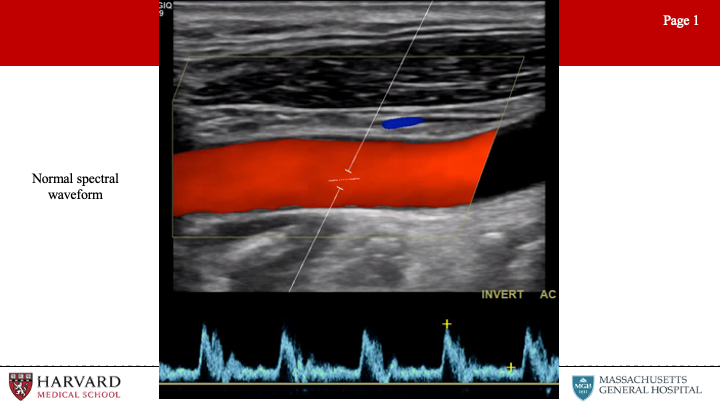
\includegraphics[width=5in]{images/vasc_lab/Slide2}

\uline{Low vs high resistance waveforms:}

Waveform profiles change depending upon the nature of the distal
vascular bed being supplied. Organs like the brain, kidneys, liver, and
spleen have constant high metabolic demand, and are therefore low
resistance vascular beds. Waveforms for arteries supplying these organs
demonstrate constant forward flow throughout the cardiac cycle because
the distal bed being supplied has low resistance leading to high
end-diastolic flow.

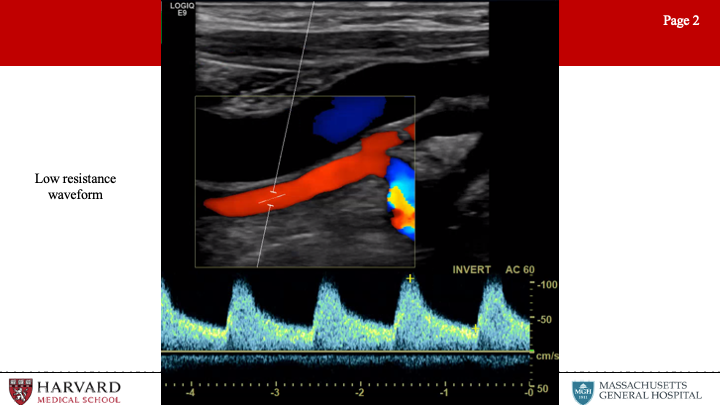
\includegraphics[width=5in]{images/vasc_lab/Slide3}

This would also be seen in the postprandial SMA. In contrast, high
resistance waveforms are seen for arteries supplying resting peripheral
muscles, fasted mesenteric beds (such as the~fasting~SMA), and the
External carotid artery. High resistance waveforms are characterized by
triphasic morphology (preprandial~ SMA or ECA).

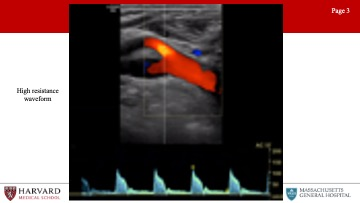
\includegraphics[width=5in]{images/vasc_lab/Slide4}

That is, sharp peaks, early diastolic flow reversal, brief forward flow
from elastic recoil of the artery, and then no flow during the remainder
of the diastolic phase.

\textbf{How does flow-limiting stenosis change the waveform?}

First let's define~\uline{Stenosis:}~A hemodynamically significant
stenosis (area reduction \textgreater50\%) will result in a doubling of velocity
from the inflow segment to the area of maximal stenosis (velocity ratio
\textgreater{} 2).

\textbf{Now what do waveforms look like AFTER a flow-limiting stenosis?}

\uline{Tardus et parvus}~refers to a pattern of Doppler ultrasound
spectral waveform resulting from arterial stenosis. The tardus et parvus
waveform is delayed with prolonged systolic acceleration (tardus) and
diminished with a small systolic amplitude and rounded systolic peak
(parvus). This phenomenon is observed downstream from the site of
stenosis. Tardus parvus in the CFA? Upstream (iliac) stenosis. Tardus
parvus in the brachial artery? Upstream (subclavian or axillary)
stenosis.

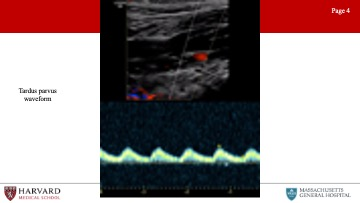
\includegraphics[width=5in]{images/vasc_lab/Slide5}

\textbf{So what will the waveform look like BEFORE a flow-limiting stenosis?}

\uline{Distal stenosis:} Distal occlusive disease will result in a high
resistance waveform, with absent diastolic flow. (Image 5: Distal
stenosis with absent diastolic flow)

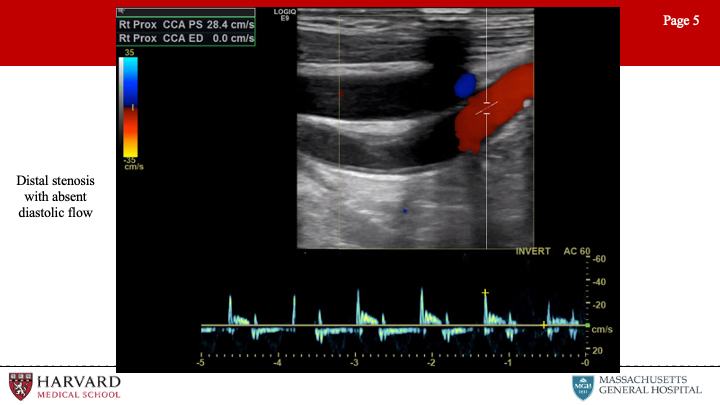
\includegraphics[width=5in]{images/vasc_lab/Slide6}

Now that we've covered the basics, let's move through by organ-~system
high-yield vascular lab studies, findings, and pathologies.We'll start
with the extracranial evaluation, a highly-tested area of vascular
ultrasonography.

\hypertarget{extracranial}{%
\section{Extracranial}\label{extracranial}}

\textbf{What does a typical extracranial evaluation involve?}

Examine CCA (2 views), ICA (2 views), ECA, vertebral arteries

\textbf{What are normal ICA and ECA waveforms?}

\uline{Normal ECA vs ICA waveform:} The external carotid artery waveform
reflects a high resistance vascular bed. This means minimal diastolic
flow. Conversely, the ICA waveform reflects a low resistance vascular
bed with antegrade diastolic flow.

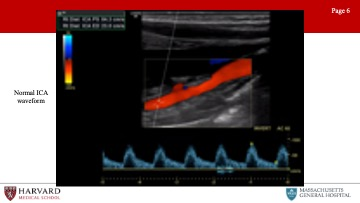
\includegraphics[width=5in]{images/vasc_lab/Slide7}

This makes sense, as the ICA is supplying the brain while the ECA is
supplying the face. Intuitively, the common carotid artery~ is a mixture
of the ICA and ECA waveform morphologies. Like the ICA with forward flow
throughout diastole, but less as compared to the ICA due to the high
resistance influence of the ECA.

Another way of differentiating the external and internal carotid
arteries is the ``temporal tap''. Tapping on the superficial temporal
artery (a branch of the ECA) will be transmitted as small pulsations in
the diastolic component of the external carotid artery.

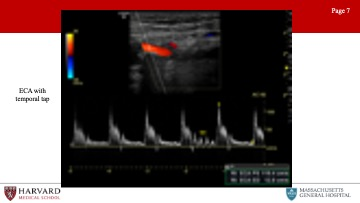
\includegraphics[width=5in]{images/vasc_lab/Slide8}

\textbf{Can you talk about diagnostic criteria for ICA stenosis?}

\uline{Parameters for ICA stenosis}: These are a few numbers that are
(unfortunately) essential to memorize for the VSITE and RPVI.

Although criteria differ between guidelines, the Carotid Consensus
Criteria, define ICA stenosis \textgreater= 70\% as a peak systolic velocity \textgreater=
230 cm/sec, EDV \textgreater{} 100 cm/sec, and ICA/CCA ratio \textgreater{} 4.0. Of note,
post-stenting criteria vary from pre-stenting criteria. Stenosis
criteria are not clearly defined for the CCA or ECA.

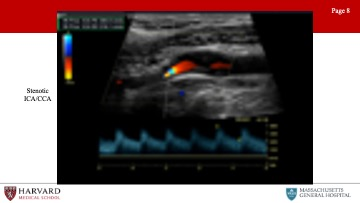
\includegraphics[width=5in]{images/vasc_lab/Slide9}

\textbf{When is surgery indicated for ICA stenosis?}

\uline{Parameters for when surgery indicated:}

Asymptomatic Carotid Atherosclerosis Study (ACAS) \textgreater60\% stenosis
asymptomatic, NASCET \textgreater50\% stenosis symptomatic

\textbf{Let's talk about other pathologies that can be visualized on
extracranial ultrasound:}

\uline{Pathologies:} Stenosis (plaque), dissection (flap), aneurysms
(rare), occlusion (no flow, do not operate), carotid body tumor
(splaying of ECA/ICA, fed by ECA branches), FMD.

FMD is frequently encountered on the VSITE/RPVI. How would this appear
on the exams?

\uline{Fibromuscular dysplasia}~of the internal carotid arteries affects
women more commonly than men. Duplex findings show a ``chain of lakes''
appearance, demonstrative of multiple septa and small aneurysms.
Velocity elevations and increased turbulence in the waveform patterns is
typically found on Doppler interrogation.

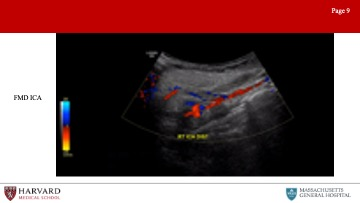
\includegraphics[width=5in]{images/vasc_lab/Slide10}

\textbf{How to treat?}

Aspirin if asymptomatic, POBA if symptomatic.

\textbf{Are there other frequently tested pathologies demonstrated on
extracranial exam?}

\uline{Subclavian steal:}~Subclavian steal occurs when a proximal
subclavian stenosis or occlusion leads to reversal of vertebral artery
flow. This causes ``stealing'' of~ blood from the posterior cerebral
circulation, and presents as vertebrobasilar insufficiency. How does
this look on duplex? Normal vertebral flow looks very similar to ICA:
antegrade low resistance waveforms with constant forward flow throughout
the cardiac cycle. As subclavian stenosis progresses, one can see
mid-systolic velocity decelerations ('bunny ears'') , and with severe
steal, there is a complete reversal of flow in the vertebral artery
towards the arm rather than towards the brain.

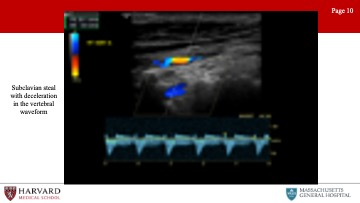
\includegraphics[width=5in]{images/vasc_lab/Slide11}

\uline{Innominate stenosis:}~A phenomenon that is related to this, is
innominate stenosis. Here again the patient will present with
vertebrobasilar insufficiency, indicative of diminished vertebral
antegrade flow, but additionally will experience right hemispheric
insufficiency secondary to diminished R ICA antegrade flow. The
right-side duplex will demonstrate flow reversal in the vertebral
artery, abnormal waveforms in the subclavian, as well as steal pattern
waveforms in the common and internal carotid arteries. The common
denominator for all of these findings is significant disease in the
innominate artery.

\hypertarget{intracranial}{%
\section{Intracranial}\label{intracranial}}

So that covers extracranial vascular lab evaluation. What about
intracranial? This is less frequently tested, so we will discuss just a
brief overview of views and some of the more commonly tested
pathologies.

\uline{\textbf{Intracranial:}}

\begin{itemize}
\item
  Three primary views: temporal, foraminal (occipital), orbital views

  \begin{itemize}
  \item
    \textbf{Temporal view:}~Used to interrogate PCA, ACA, MCA, and ICA.
    The~MCA, ICA and PCA flow direction is towards the probe, the~,
    The ACA~flow direction~is AWAY.
  \item
    \textbf{Occipital view:}~Basilar and vertebral arteries (both away).
  \item
    \textbf{Orbital view:}~Ophthalmic and ICA
  \item
    Arteries differentiated by depth. MCA 3-6 cm, everything else
    deeper.
  \end{itemize}
\end{itemize}

\textbf{What are some frequently tested pathologies that are identified on
TCD?}

Indications often tested:

\begin{itemize}
\item
  \uline{MCA spasm (severe PSV\textgreater200)}: Can be seen in sickle cell
  disease with studies indicating a strong correlation between mean
  velocities of \textgreater200cm/s and the rate of stroke in children with
  sickle cell disease. With blood transfusions, stroke risk can be
  reduced from \textgreater10\% to \textless1\% per year.
  \citep{bulasTranscranialDopplerTCD2000}
\item
  \uline{Cerebral ischemia during CEA:}~Comparing transcranial Doppler
  sonography, near-infrared spectroscopy, stump pressure measurement,
  and somatosensory evoked potentials, cerebral ischemia was most
  accurately predicted by the percent change in transcranial Doppler
  detected middle cerebral artery velocity. Detection of a greater
  than 50\% drop in middle cerebral artery velocity using transcranial
  Doppler is 100\% sensitive for detecting cerebral
  ischemia.\citep{moritzAccuracyCerebralMonitoring2007}
\item
  TCD can also demonstrate microemboli (high spikes on spectral
  doppler) during CEA
\end{itemize}

\hypertarget{upper-extremity}{%
\section{Upper Extremity}\label{upper-extremity}}

Having covered head and neck vasculature, let's move on to peripheral
vasculature. This is a huge area both on the VSITE/RPVI and in practice.
In this section we'll cover first the upper, then the lower extremity
vasculature.

\textbf{So first, what are characteristics of waveforms in the peripheral
vasculature?}

\uline{Peripheral}: Normal waveforms are indicative of high resistance
distal beds, so we would expect triphasic waveforms

\textbf{What are normal arterial parameters in the upper extremities?}

\uline{Upper Extremity:}

\begin{itemize}
\tightlist
\item
  \textbf{Normal parameters:}~Normal pressure gradient between the right
  and left brachial pressures is \textless20 mmHg. Normal finger pressure
  is \textgreater80\% of the ipsilateral brachial systolic pressure. So a normal
  digital brachial index is \textgreater=0.80. A gradient between digits of \textgreater15
  mmHg is considered abnormal.~
\end{itemize}

\textbf{Let's talk about some of the most frequently tested pathologies,
starting with arterial TOS.}

\uline{Arterial TOS:}~Results from compression of the subclavian artery
at the level of the first rib within the scalene triangle. Arterial TOS
testing is done by placing a sensor, most often photoplethysmography
(PPG), on one finger of each hand, recording the resting waveforms and
then recording while during maneuvers to evoke arterial compression in
the thoracic outlet.

\textbf{Can you tell us a little more about PPG testing?}

\uline{Photoplethysmography (PPG)}~uses an infrared light to illuminate
superficial tissue. The reflection is received by a photosensor, and
amplitude of the reflected light is proportional to the volume of red
blood cells in the sample area. A normal digital arterial PPG has a
brisk upstroke with a narrow systolic peak, and a dicrotic notch on the
downslope during diastole.

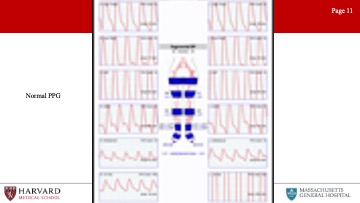
\includegraphics[width=5in]{images/vasc_lab/Slide12}

Digital PPGs change with progression of peripheral vascular disease. The
first changes are a loss of amplitude and loss of the dicrotic notch.
More advanced disease~findings include a flattened systolic peak and a
prolonged upstroke. Significant arterial TOS is suggested when there is
a loss or persistent flattening of the digit waveforms during any of the
positional changes that can compress the subclavian artery (either with
the clavicle, first rib and scalene muscle). However, it should be noted
that up to one-third of patients without arterial TOS may have some
degree of subclavian artery compression with positional maneuvers.

\textbf{What are other diseases affecting the upper extremity?}

\uline{Raynaud's:}~Vasospastic disorder characterized by temporary
vasospasm. Diagnosis may be assisted by decrease in digital waveforms
with immersion of the hand in cold water.

\uline{Thromboangiitis obliterans:}~Is a segmental non-atherosclerotic
inflammatory disorder characterized by microthrombosis that primarily
involves the small- and medium-sized arteries. Ultrasonography may
demonstrate the classical ``corkscrew'' collateral development at the
level of occlusion. TA has a male predominance and first line treatment
is smoking cessation.

\hypertarget{hemodialysis-access}{%
\subsection{Hemodialysis Access}\label{hemodialysis-access}}

Before we segue to the lower extremities, this is a good time to discuss
an entity frequently tested on the VSITE, and that constitutes for many
vascular surgeons a notable portion of their practice, and that is
hemodialysis access, and specifically fistulas.

\uline{Fistulas}: Ultrasound is one of the key modalities used in
identifying suitable anatomy for fistula placement, suitability of a
fistula for dialysis, and finally complications of fistulas.

\textbf{So first, assessment for fistula placement:}

The optimal configuration for an AVF is determined on the basis of vein
mapping and noninvasive studies. Veins should measure \textgreater3 mm in diameter
(\textgreater2.5 mm may be acceptable, as veins are likely to dilate under
anesthesia), and there should be no arterial inflow stenosis or venous
outflow stenosis. Duplex ultrasound arterial imaging can be performed at
the same time as vein mapping and can provide important predictors of
fistula maturation, such as arterial diameter and flow. The minimal
arterial lumen diameter is 2 mm.

\textbf{How can we tell if a fistula is ready to be used for hemodialysis
access?}

\uline{Assessment for fistula suitability for dialysis:}~Rule of 6's: At
six weeks post-creation the diameter of the fistula should be at least 6
mm and the depth no more than 0.6 cm. The flow rate should be at least
600mL/min, and the length of the fistula should be 6 cm to allow for a
successful two-needle dialysis.

\textbf{What do normal fistula spectral waveforms look like?}

\uline{Waveform:}~The arterial waveform should demonstrate very low
resistance throughout diastole. End diastolic velocity should be one
half to two thirds of peak systolic velocity in a well-functioning
fistula. As a side note, this is also what one would see in an
iatrogenic arteriovenous fistula, as between the femoral artery and
vein.

\textbf{Let's discuss commonly encountered complications and pathologies
identified in association with fistulas:}

\uline{Pseudoaneurysms:}~Pseudoaneurysms commonly occur when a puncture
fails to seal and the blood is contained by the surrounding soft tissue.
As in other locations, pseudoaneurysms are defined on imaging by a
communicating neck between the arterial vessel and pseudoaneurysmal sac
with ``to-and-fro'' waveform at duplex. While small pseudoaneurysms can be
managed without intervention or surgery, larger pseudoaneurysms,
pseudoaneurysms associated with infection or overlying skin changes or
bleeding may require excision and repair.

\uline{Steal syndrome:}~Hemodialysis-related steal, also known as
access-related hand ischemia, which may occur in over half of all
patients undergoing access creation. Steal is characterized by
retrograde diastolic flow distal to the donor artery. Of note, reversal
of flow in and of itself is not sufficient to cause distal ischemia with
an intact palmar arch. This is commonly seen after access creation and
represents physiologic steal phenomenon, rather than symptomatic steal
syndrome. Digital pressures \textless60 mm Hg are highly sensitive and specific
for predicting steal. Patients who have no symptoms (Grade 1
access-related hand ischemia), may be closely monitored without any
intervention. How do we treat more severe steal? Flow rate measurements
of the fistula can help determine the optimal treatment (banding,
revision using distal inflow, distal revascularization with interval
ligation, proximalization of arterial inflow or ligation of the
fistula).

\textbf{So steal can occur in the context of high fistula output, can we talk
a bit about low fistula flow, as from stenosis?}

\uline{Central venous stenosis:} Venous outflow stenosis is the most
common reason for arteriovenous graft failure. A low flow rate results
in recirculation during the dialysis session. Venous obstruction
manifests as arm swelling, and with central venous stenosis may present
with collateral development over the upper extremity and chest wall.

\uline{Stenosis of fistula:}~Arterial and mid-graft stenosis can also
cause complications, but are less common than venous stenosis. Stenosis
on imaging will be represented by narrowing of luminal diameter on
b-mode ultrasound, high-resistance waveform proximal to the stenosis,
and tardus parvus waveform distal to the stenosis.

\hypertarget{lower-extremity}{%
\section{Lower Extremity}\label{lower-extremity}}

\textbf{Can you please tell us about some of the diagnostic modalities that
are used to examine perfusion in the lower extremities?}

\uline{ABIs:}~Ankle-brachial index measurement requires calculating the
ratio of the highest ankle systolic pressure (posterior tibial artery or
dorsalis pedis) over the highest brachial systolic pressure. Regardless
of whether you're doing the R or L ABI, use the higher arm pressure for
both ratios. Normal ABI \textgreater0.9, severe disease indicated by ABI\textless0.5, and
CLI by ABI\textless0.3. The ankle-brachial index in diabetic patients is
frequently unreliable due to incompressibility of the tibial vessels at
the level of the cuff secondary to calcification. Consequently, toe
pressures are mandatory in all patients with diabetes mellitus. Normal
TBI\textgreater0.7.

\uline{TcPO2:}~When there is significant tissue loss, preventing TBI
measurement, another option is transcutaneous oximetry
(TcPO2).~~Transcutaneous oximetry is a non-invasive method of measuring
the tissue partial pressure of oxygen through a heated sensor on the
skin. A TcPO2 value of 40 mmHg is the critical value below which wound
healing is impaired and ischemia develops.

\textbf{Are there other non-invasive ways of determining extremity
perfusion?}

\uline{PVRs:}~Pulse volume recordings. Normal PVR waveforms have a rapid
upstroke, sharp peak, prominent dicrotic notch and downslope. Typically
4 cuffs. High thigh cuff should be 30\% greater than brachial pressure,
hence a thigh-brachial index of 1.3 is normal. However, ABI/PVRs may not
demonstrate significantly abnormal values/waveforms in individuals with
single level disease.

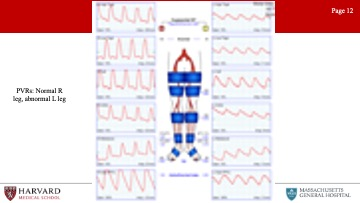
\includegraphics[width=5in]{images/vasc_lab/Slide13}

\uline{Exercise Test:}~During exercise testing, patients are placed on a
treadmill after baseline resting ABIs are measured. The patient is then
asked to walk for 5 minutes or until physical discomfort requires test
cessation. The point when a patient stops is defined as the absolute
claudication distance. Diagnostic criteria for a positive test include a
drop-in ankle pressure of greater than 20 mmHg from baseline, drop in
ABI greater than 0.2 from baseline, or inability of ankle pressures to
return to baseline after 3 minutes.

\textbf{So just to briefly summarize, what are parameters associated with poor
wound healing?}

\uline{Parameters associated with poor wound healing:}~Considering these
various testing modalities, what are factors associated with poor
likelihood of wound healing? An ankle pressure \textless50 mmHg, ABI \textless{} 0.40,
TcPO2 \textless20 mmHg, or a toe pressure \textless20 mmHg are considered predictive
of non-healing.

\textbf{Ultrasound is frequently used for graft surveillance. Can you talk
about graft surveillance parameters?}

\uline{Restenosis/Graft surveillance}: Suggested ultrasound surveillance
bypass graft begins immediately after surgery and then continues at 3,
6, and 12 months and then every 6 to 12 months thereafter. A velocity
ratio (Vr) is defined as the peak systolic velocity (PSV) at the site of
a stenosis divided by the PSV in a normal vessel segment proximal to the
stenosis. The highest risk for graft thrombosis, and highest cause for
concern is suggested by PSV \textgreater300 cm/s, Vr \textgreater3.5, a graft flow velocity
\textless45 cm/s or a drop in ABI \textgreater0.15.\citep{bandykHemodynamicsVeinGraft1988}

\hypertarget{pathologies}{%
\subsection{Pathologies}\label{pathologies}}

\textbf{Let's talk about pathologies frequently encountered in the lower
extremities:}

\uline{Pseudoaneurysms (particularly femoral):}~Gray-scale
ultrasonography demonstrates a hypoechoic cystic structure adjacent to
an arterial supply. Color Doppler typically demonstrates a ``yin-yang
sign'' within the pseudoaneurysm sac. The hallmark ultrasound sign is
identification of a neck between the sac and the feeding artery with a
``to-and-fro'' spectral Doppler waveform measured at the neck. This
represents the flow in and out of the PSA during systole and diastole.

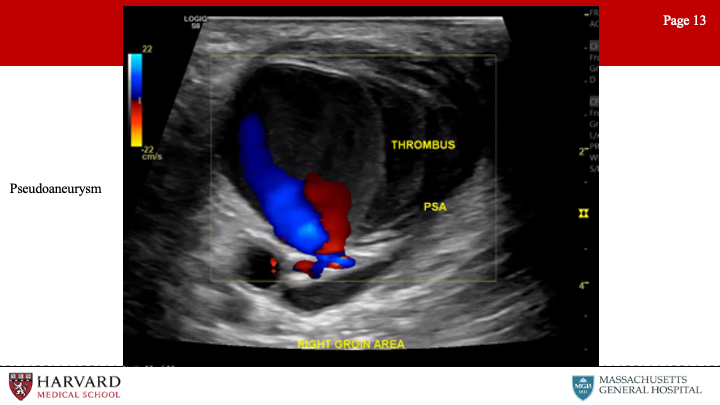
\includegraphics[width=5in]{images/vasc_lab/Slide14}

\uline{Dissections:}~Characteristic ultrasound findings on color Doppler
include a parallel blood-flow channel that separates the true and false
lumen.

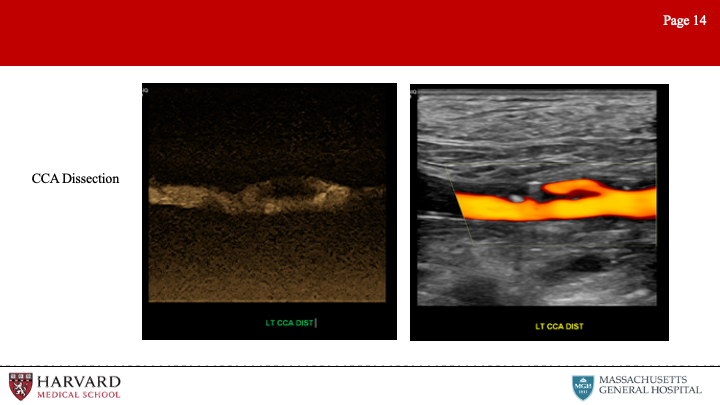
\includegraphics[width=5in]{images/vasc_lab/Slide15}

Of note, if the false lumen is filled by a thrombus, it may not
distinguishable from an intramural hematoma or noncalcified plaque

There are several disease pathologies that are frequently tested
relating to the popliteal fossa. Can you talk briefly about these?

\uline{Adventitial cystic disease:}~This is a rare (but often tested)
pathology. Adventitial cystic disease is a nonatherosclerotic etiology
of claudication, most often affecting the popliteal artery in the lower
extremity and leading to stenosis or occlusion. Duplex imaging of the
popliteal artery will demonstrate an anechoic~\emph{intraluminal}~region with
a smooth contour and stenosis documented by velocity increase on
spectral doppler.

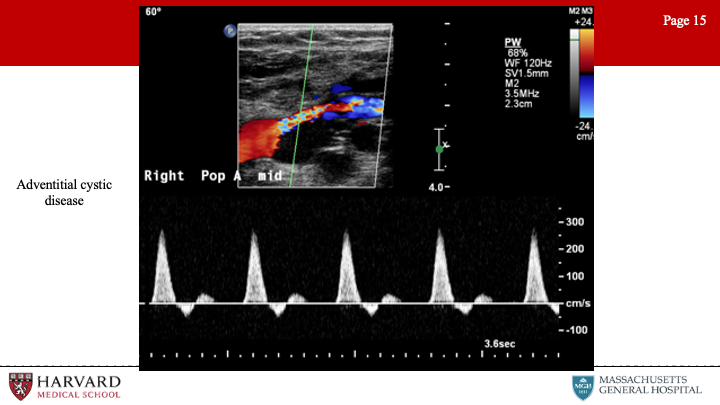
\includegraphics[width=5in]{images/vasc_lab/Slide16}

This is not to be confused with a

\uline{Bakers Cyst}\textbf{:}~which is a benign, cystic structure found in the
popliteal fossa and arising from the joint capsule. Flexion of the knee
may result in compression of the popliteal artery by the cyst. On b-mode
ultrasound, a well-defined, anechoic~ cystic structure with a `neck'
extending into the joint space between the semimembranosus tendon and
the medial head of the gastrocnemius will be identified.

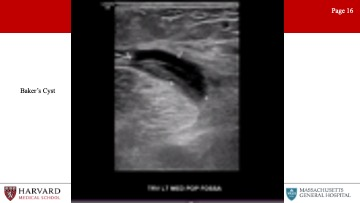
\includegraphics[width=5in]{images/vasc_lab/Slide17}

\uline{Popliteal entrapment syndrome:}~decrease in ABI or loss of distal
pulses with passive dorsiflexion or active plantar flexion of the foot
caused by compression of the popliteal artery by the gastrocnemius.

\hypertarget{abdominal}{%
\section{Abdominal}\label{abdominal}}

\hypertarget{aorta}{%
\subsection{Aorta}\label{aorta}}

\textbf{AAA:}~Ultrasound screening of a AAA is non-invasive, accurate, and
cost-effective. Sensitivity of 98\% and specificity of 99\% for AAA
diagnosis. Size criteria for AAA repair is 5.5 cm men, 5.0-5.5 cm in
women, measured outer~wall to outer~wall cross-sectional diameter.

\textbf{Can ultrasound be used for graft surveillance s/p EVAR?}

\uline{S/p EVAR:}~Surveillance color duplex ultrasound is safe if CT
imaging at 1 year exhibits no sac growth, graft migration, or endoleak
(or stable type II endoleak). Can detect endoleaks, sac expansion, and
limb occlusion. Migration difficult to assess given challenge of renal
arteries visualization in a long axis view of the aorta.

\textbf{What other pathologies can be identified on ultrasound evaluation of
the abdomen?}

\uline{CIA aneurysms:}~SVS defines CIA aneurysms as any permanent,
localized dilatation of the iliac artery \textgreater1.5 cm in diameter (diameter
1.5x the normal diameter)

\uline{Para-anastomotic pseudoaneurysms:}~As previously discussed
(reported in up to 0.5\% to 10\% of cases)

\uline{Penetrating aortic ulcers:}~Describes an ulcerating
atherosclerotic lesion that penetrates the intima and progresses into
the media. Associated with atherosclerotic plaque on ultrasound

\uline{Dissections:}~(as already discussed) a dissection flap is usually
identified and color flow demonstrates dual channels (true and false
lumens). Turbulent flow patterns are frequently encountered.

\hypertarget{mesenteric-vasculature}{%
\subsection{Mesenteric Vasculature}\label{mesenteric-vasculature}}

So far we have steered clear of the mesenteric vasculature. But this is
an area frequently encountered on exams. Let's start with mesenteric
vessel stenosis.

\textbf{Celiac and SMA stenosis:}~May present as chronic mesenteric
ischemia.~PSV \textgreater275 cm/s in the SMA or \textgreater200 cm/s in the celiac artery
indicates \textgreater=70\% stenosis. Normal SMA Doppler waveforms in the fasting
patient show high resistance waveform, PSV \textless275 cm/s and no spectral
broadening. In the postprandial state, the waveform becomes low
resistance, with a slightly increased PSV and little to no spectral
broadening. Significant SMA stenosis may be differentiated by the
presence of spectral broadening and elevated PSV and EDV. Distal to the
stenosis, one would expect a tardus parvis waveform. EDV \textgreater45 in SMA or
\textgreater55 in celiac are predictive of stenosis (would expect higher diastolic
flow in celiac trunk given low resistance vascular bed of liver and
spleen).

\textbf{What other mesenteric vessel pathologies may be identified on vascular
ultrasound?}

\uline{Dissections:}~Rare without concomitant aortic dissection.

\uline{Aneurysms:}~Rare. Repair \textgreater2 cm celiac, hepatic, SMA aneurysms and
\textgreater3 cm splenic and renal.

\uline{Median arcuate ligament syndrome:}~MALS can cause significantly
elevated velocities at the origin of the celiac artery. Testing is for
reversible mechanical compression, as opposed to a fixed lesion from
atherosclerotic disease. During deep inspiration or in the upright
position, celiac velocities should normalize if stenosis is secondary to
MALS.

\textbf{So I recognize that we are jumping ahead here discussing venous
circulation, but as this represents another component of a mesenteric
vascular exam, let's discuss portal venous ultrasonography.}

\uline{Portal vein:}~Normal portal venous flow is hepatopetal (toward the
liver), whereas abnormal portal venous flow is hepatofugal (away from
the liver). (The root ``fugua'' means to flee, or flight). Flow should be
in the same direction as the hepatic artery. Other abnormalities that
may be visualized are portal vein thrombosis (often associated with
portal venous hypertension in patients with chronic cirrhosis,
hepatitis, or hepatocellular carcinoma). Acute portal vein thrombosis on
ultrasound demonstrates dilatation of the portal vein with hypoechoic
intraluminal thrombus. Chronic portal vein thrombosis is characterized
by a contracted vein with heterogeneous/hyperechoic echoes and may be
associated with collateral formation.~ Can also assess for hepatic
artery stenosis/thrombosis and for functioning of TIPS (transjugular
intrahepatic portosystemic shunt).

\textbf{Awesome, and so before jumping fully into venous circulation, let's
complete our discussion of abdominal ultrasound evaluation with a
discussion of the renal vasculature.}

\uline{Renal Pathologies:}~ostial (atherosclerotic) vs mid-artery (FMD)

\uline{Atherosclerotic stenosis:}~PSV\textgreater200 cm/s predictive of \textgreater60\%
stenosis. Renal artery-to-aortic PSV ratio (RAR) \textgreater3.5 also correlates
with a \textgreater60\% stenosis. The renal resistive index (RRI) is calculated as
the RA PSV-EDV/PSV. The RRI (\textgreater0.8) is an indicator of intrinsic
parenchymal renal disease.

\uline{FMD:}~As discussed for the carotids, FMD manifests as beaded
lesions in medium and small arteries, with the renal arteries the most
commonly affected. Ultrasound demonstrates increased PSV in the mid and
distal renal artery. Stenoses in the mid and distal renal artery are
suggestive of FMD, atherosclerotic disease is primarily ostial in
nature.

\hypertarget{venous}{%
\section{Venous}\label{venous}}

\textbf{Venous Exam:}~Uses a linear transducer. Complete deep venous reflux
duplex examination includes color and pulsed wave spectral doppler
imaging. Spontaneous Doppler waveforms as well as provocative maneuvers
are recorded in the common femoral, femoral, popliteal, and tibial deep
veins. Superficial veins (GSV, SSV, and perforator veins) are evaluated
with provocative maneuvers to test valve competency. Diameters are also
included for superficial veins. Transverse B-mode images are used for
vessel compression (as when looking for thrombus) to ensure that the
vein is fully compressible under probe pressure as opposed to simply
slipping out of view, as may occur in longitudinal views. Reflux exam
should be performed with a patient standing, with assessment performed
on the non weight-bearing leg.

\textbf{We've talked extensively about normal arterial waveforms; what do
normal venous waveforms look like?}

\uline{Normal venous waveforms:}~Normal flow patterns of iliac and
femoral veins demonstrate phasicity and should augment with distal
compression. In the upper extremity central veins, doppler waveforms
normally demonstrate pulsatility and phasicity.

\textbf{What does this mean? Pulsatility, phasicity, and augmentation}?

\textbf{Pulsatility:}~Refers to changes in the venous waveform in accordance
with the cardiac cycle. Pulsatility is normal in the upper extremity
veins central veins, given their proximity to the heart.

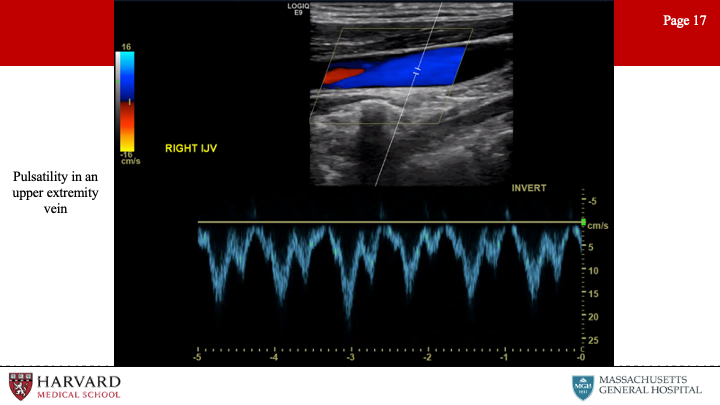
\includegraphics[width=5in]{images/vasc_lab/Slide18}

This is an abnormal finding in the lower extremity veins, and may be a
sign of pulmonary hypertension, right heart failure, or tricuspid
regurgitation.

\textbf{Phasicity:} (also called respiratory phasicity) is variation in the
waveform with respiration. This results from increasing and decreasing
intrathoracic pressures secondary to respiration. Phasicity is an
indicator of a patency proximal to the point of measurement. So if we
see lack of phasicity (continuous flow) in the left femoral vein but
normal phasicity in the right, we would be concerned for left iliac vein
occlusion or stenosis. If we saw absence of phasicity (continuous flow)
in the bilateral femoral veins, we would be concerned for IVC
obstruction or stenosis.

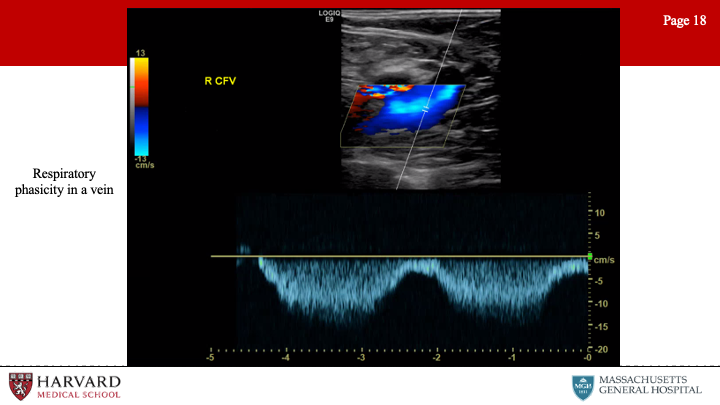
\includegraphics[width=5in]{images/vasc_lab/Slide19}

\textbf{Augmentation:}~Distal compression that augments forward flow. For
example, if we are measuring flow at the femoral vein and we squeeze the
calf and we see augmentation in the waveform, this indicates lack of
occlusion in the venous system from the knee to the probe.

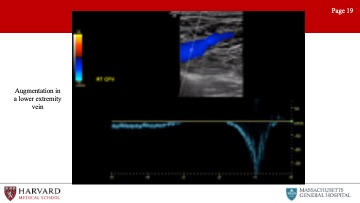
\includegraphics[width=5in]{images/vasc_lab/Slide20}

\textbf{What are venous pathologies that are commonly tested/encountered?}

\uline{Reflux:}~Venous reflux due to valvular incompetence is best
assessed with duplex scanning in the upright position. Reflux in the
common femoral vein and the saphenofemoral junction may be elicited with
a Valsalva maneuver (which increases intra-abdominal pressure), but
release of a pneumatic cuff compression is a more reproducible method.
Reflux is identified as reverse flow - that is, away from the heart -
following valsalva or release of the compression cuff.

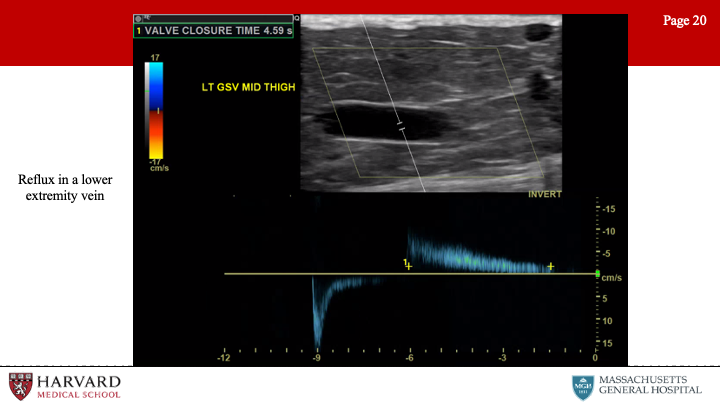
\includegraphics[width=5in]{images/vasc_lab/Slide21}

Consensus guidelines suggest a cutoff value of 1 second for abnormally
reversed flow (reflux) in the femoral and popliteal veins and of 0.5
seconds for the great saphenous vein, small saphenous vein, tibial, and
deep femoral veins.

\uline{Perforator veins:}~Perforator veins connect the deep and
superficial venous systems, penetrating the deep fascia overlying the
muscle.~ Size \textgreater3.5 mm and reflux \textgreater350 ms (deep to superficial) is
associated with perforator reflux. Pathological perforator = in
association with a healed or non-healed ulcer.

\textbf{What are some other examples of reflux?}

\uline{Ovarian vein reflux:}~The ultrasound evaluation of pelvic
congestion syndrome is performed in steep reverse Trendelenburg and
standing positions with a low-frequency probe. Reflux is identified
during the Valsalva maneuver. There are no validated criteria for the
duration of reflux. Rather, an ovarian vein diameter \textgreater6 mm is
considered significant.

\uline{May Thurner}\textbf{:}~Also known as iliac vein compression syndrome,
refers to a chronic compression of the left~\href{https://radiopaedia.org/articles/common-iliac-vein?lang=us}{common iliac
vein} by the
overlying right~\href{https://radiopaedia.org/articles/common-iliac-artery?lang=us}{common iliac
artery}~(CIA),
with or without~\href{https://radiopaedia.org/articles/deep-vein-thrombosis?lang=us}{deep venous
thrombosis}.
Notably, patients present with unilateral (left) lower extremity edema
and pain, varicosities, DVT or venous ulcers. Intravascular ultrasound
will demonstrate \textgreater50\% stenosis of the iliac vein from compression.
Distal waveforms will demonstrate absence of phasicity if
obstruction/stenosis is severe with continuous flow.

\textbf{Ok, let's transition from reflux to thrombosis:}

\uline{Thrombosis:}~Characteristics of acute thrombus are an echolucent
and incompressible thrombus in a thin-walled vein with significant
distension.

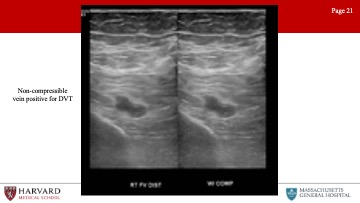
\includegraphics[width=5in]{images/vasc_lab/Slide22}

Acute thrombus typically causes the vein to dilate with a diameter
greater than the diameter of the adjacent artery. Venous wall
thickening/scarring, a contracted vein, recanalization, and
collateralization is found in chronic thrombosis.

\textbf{Let's discuss 2 Specific examples of venous thrombosis: VTOS and
EHIT}

\uline{Venous TOS:}~Venous thoracic outlet syndrome is thrombosis or
severe stenosis of the subclavian or axillary veins secondary to chronic
extrinsic mechanical compression. Repetitive injury to the subclavian
vein at the level of the costoclavicular space results in chronic injury
to the veins. Venous duplex may show a dilated, non-compressible vein
consistent with an acute subclavian vein DVT, or lack of
pulsatility/phasicity if obstruction/stenosis is more centrally located.

\uline{EHIT or Endovenous Heat Induced Thrombosis:}~S/p endovenous
thermal ablations (RFA or laser ablation) of the GSV. 4 Grades: Grade 1
is thrombus in the GSV up to the level of the CFV. If \textless{} 50\% of the CFV
lumen is involved this is EHIT grade 2. EHIT grade 3 is extension into
the CFV occupying \textgreater50\% of the lumen and grade 4 is occlusion of the
CFV.

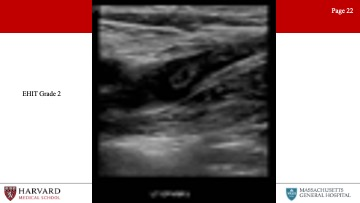
\includegraphics[width=5in]{images/vasc_lab/Slide23}

EHIT grades 3-4 are typically treated with anticoagulation to reduce
risk of PE. To minimize the risk of EHIT, the catheter should be
positioned at least 2 cm from the saphenofemoral junction.

\hypertarget{artifacts}{%
\section{Artifacts}\label{artifacts}}

Finally, let's wrap up this episode with a discussion of imaging
artifacts. These are frequently encountered and tested in vascular
ultrasound, and it is important to recognize imaging artifacts in order
to prevent incorrect interpretation.

\textbf{Acoustic shadowing:}~Shadowing on an ultrasound image is
characterized by a signal void behind structures that strongly absorb,
reflect, or refract ultrasonic waves.

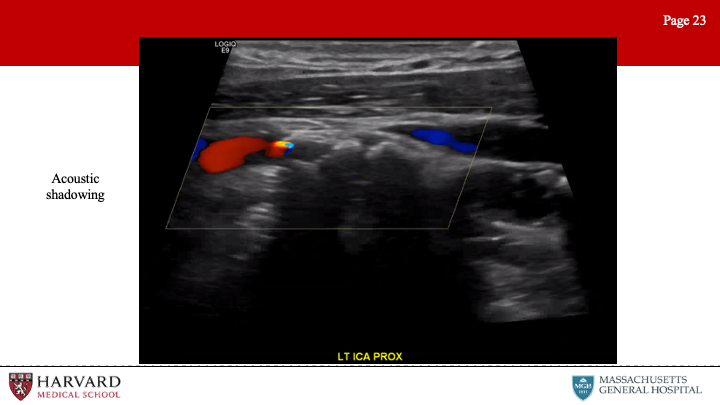
\includegraphics[width=5in]{images/vasc_lab/Slide24}

Practically speaking, this most typically occurs deep to strongly
reflective surfaces such as calcified plaques, and appears as a ``dark
area'' beneath the plaque.~\textbf{Acoustic enhancement}~is essentially the
inverse situation, and appears as a ``bright area'' deep to structures
that transmit ultrasound waves exceptionally well. This can happen deep
to fluid-filled structures such as cysts.

\textbf{Mirroring}: A mirror-image artifact is caused by reverberation of
ultrasound and shows structures that exist on one side of a strong
reflector as also being present on the other side of the reflector.

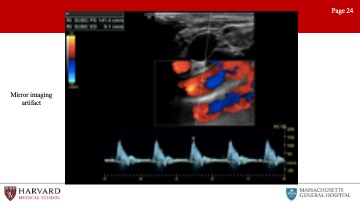
\includegraphics[width=5in]{images/vasc_lab/Slide25}

This is often seen around the pleura and the diaphragm, due to the
strong reflection of ultrasound from the air-filled lung. These
artifacts can occur in both B-mode imaging where you see the mirrored
image and Doppler, in which you see the mirrored waveform.

\textbf{Refraction:}~A refraction artifact is the result of ultrasound waves
passing through tissues with different propagation velocities (such as
air and water) and causes a structure to be improperly positioned
laterally in the image. This is the phenomenon that results in a straw
appearing bent when in a glass of water.

\textbf{Speed artifact:}~Depth determination by an ultrasound machine is
based on calculations using an average propagation velocity of sound in
soft tissue of 1540 m/s. If the ultrasound wave passes through a medium
at a different speed than predicted by the machine, an inaccurate image
depth will be displayed. If the ultrasound passes less quickly through
the material than soft tissue (as occurs in air or fluid), then the
image will be displayed deeper than the true depth. In practical
application, this is what causes a ``bayonet'' sign, or apparent bending
of a needle when it passes from soft tissue into a cystic structure.

\textbf{Inappropriate color gain:}~Overly gained images will show ``speckling''
in areas in which no flow is present (such as in soft tissue).

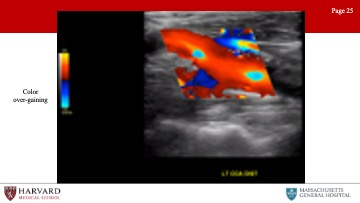
\includegraphics[width=5in]{images/vasc_lab/Slide26}

Under-gaining will result in reduced sensitivity to low velocity flow.

\textbf{Inappropriate angle correction:}~Make sure the angle correction
cursor is centered in the vessel and parallel to the walls, otherwise
the Doppler velocity measurement will be incorrect.

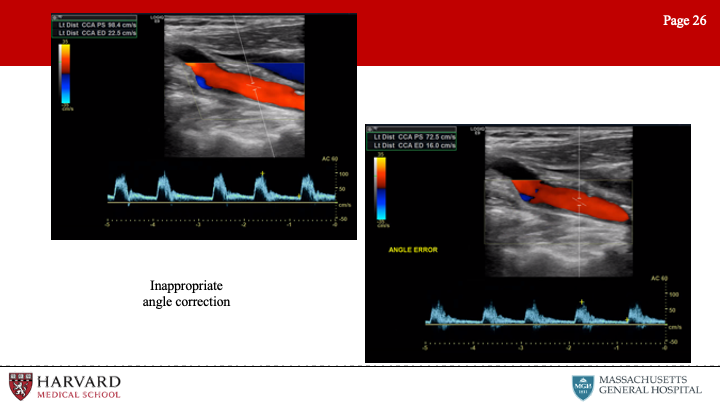
\includegraphics[width=5in]{images/vasc_lab/Slide27}

Finally, can we talk about aliasing, as I feel like this comes up a lot
on exams:

\textbf{Aliasing:}~Unlike~\href{https://radiopaedia.org/articles/continuous-wave-doppler?lang=us}{continuous wave
Doppler},
pulsed wave and color flow Doppler are characterized by rapid pulses of
ultrasound waves (at a rate called the pulse repetition frequency).
The~\href{https://radiopaedia.org/articles/nyquist-limit?lang=us}{Nyquist
limit}~defines
the frequency at which aliasing will occur, as equal to the PRF/2. So
what does this mean practically? In pulsed wave doppler, if the velocity
of blood is greater than ½ the PRF, the peak velocity will be cut off,
and wrapped around to the bottom of the scale.

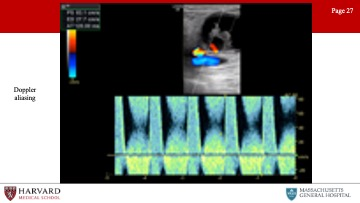
\includegraphics[width=5in]{images/vasc_lab/Slide28}

This results in inaccurate measurement of peak velocities, and may be
remedied by increasing the PRF and hence the scale. In color flow
doppler, aliasing appears as red to blue hues without separation of a
black region indicating no flow. This occurs in areas of high velocity
(such as immediately post-stenosis). This can be remedied with an
increase in the color scale. Of note, if asked to determine the
direction of blood flow in a vessel demonstrating aliasing, one should
assess the flow in low-velocity areas of blood flow, as seen along
vessel walls.

\hypertarget{endovascular}{%
\chapter{Endovascular}\label{endovascular}}

\hypertarget{vascular-access}{%
\section{Vascular Access}\label{vascular-access}}

\textbf{29 Apr 2020}: \emph{Sammy Siada, MD and Rafael Malgor, MD}

Endovascular procedures are the cornerstone of any modern vascular
surgery practice. Because most endovascular procedures are performed
percutaneously using arterial or venous access, it is critical that
vascular surgeons are facile with various techniques and devices used
for endovascular access. Today we'll be discussing the various access
sites, techniques for access, closure devices, and complications.

\textbf{What factors play a role when choosing a site for access?}

The factors to think about when thinking about which vessel to access
are:

\begin{itemize}
\item
  The appropriateness of the access site the procedure performed
\item
  Ability to obtain hemostasis at the conclusion of the procedure
\item
  Ability to convert to open if necessary
\item
  Effects of access on the tissues supplied by the accessed vessel and
  distal limb perfusion
\end{itemize}

\textbf{What makes a vessel appropriate for access?}

One of the most important factors when planning your access is the size
of the vessel. The vessel needs to be able to accommodate the catheters
and devices that will be used to perform the procedure. For instance, a
brachial artery with less than 4mm diameter should not be accessed by a
large bore sheaths, such as a 12Fr sheath.

The vessel also needs to be a in a location that can allow access to the
target vessel of interest. Additionally, the vessel needs to have an
area that is relatively healthy to access the vessel safely and minimize
complications. Heavily calcified vessels especially those with anterior
wall calcification might not be appropriate for access.

\textbf{What about the ability obtaining hemostasis at the end of the
procedure?}

The ability to obtain hemostasis is critical to be able to perform
endovascular procedures safely which is one reason why the common
femoral artery is the most commonly accessed vessel.

Hemostasis is most commonly achieved through manual compression by
compressing the artery against the femoral head. The brachial artery can
also be compressed against the humerus, but because it's a more mobile
vessel, compression is less effective and can lead to hematoma or
pseudoaneurysm formation which may necessitate an operation to prevent
compression of the median nerve

Patients who will need to be uninterruptedly anticoagulated peri and
postoperatively pose a challenge to hemostasis. The use of closure
devices is very important in these situations to prevent access
bleeding.

A variety of closure devices can also be used to assist in hemostasis,
each with their own inherent advantages and disadvantages. In general,
closure devices are contraindicated in small diameter and heavily
calcified vessels.

\textbf{In any minimally invasive procedure, there is always a chance that you
may need to convert to open. How does converting to open play a role in
vascular access?}

Conversion to open is uncommon with vessel access accounting for \textless5\% of
the cases. Sometimes a large sheath is accidentally pulled out and a
cutdown becomes necessary to repair the artery. Closure devices aren't
100\% effective in hemostasis and may also require a cutdown for
definitive control if they fail, especially when obtaining large bore
access.

This makes choosing the right vessel critical. For example, if a large
sheath is accidentally pulled out of the CFA during an EVAR, the repair
can be done through a straightforward groin cutdown. In contrast, the
subclavian artery is rarely accessed percutaneously because converting
to open would require a more challenging peri-clavicular incision or
even a thoracotomy for repair.

\textbf{Large diameter sheaths are often used, particularly in aortic
procedures. These sheaths can be occlusive which can result in
downstream tissue ischemia. What considerations should be taken when
thinking about downstream tissue ischemia?}

When performing diagnostic procedures using small diameter sheaths and
catheters, anticoagulation may or may not be necessary depending on how
diseased the access vessel is.

However, when using large devices (e.g.~in EVARs), the sheaths can be
partially or completely occlusive which mandates full anticoagulation to
prevent thrombosis. The other thing to consider is the length of time
that the sheath remains in the vessel as the leg can only tolerate
ischemia for 4-6 hours. This is usually pertinent when performing
complex endovascular aortic procedures.

To minimize downstream tissue ischemia, a large bore sheath should be
pulled back to decrease the length of vessel obstruction by its shaft in
order to unblock proximal vessel collateral branch vessels. For
instance, when performing an aortic procedure through a femoral access
attempt to pull the sheath back into the external iliac artery to
increase distal limb perfusion through the internal to femoral artery
collateral branch vessels.~~

The long story short is to be liberal with anticoagulation when there is
reduced flow in the vessel such as the iliofemoral system during EVAR or
tibial access

\textbf{Do the principles that we've described also apply to veins?}

The same principles apply but there are some notable differences between
arterial and venous access.

Veins are a low-pressure system, so hemostasis is easier to achieve and
hemorrhagic complications are much less common. However, this poses a
challenge during access as there is less radial force keeping the vein
open making the vein more susceptible to compression by the ultrasound
probe and the needle.

If a large bore sheath is necessary to perform a venous procedure, a
suture-mediated closure device can be utilized to achieve hemostasis
especially in patients that will be kept fully anticoagulated

Additionally, a syringe may be needed to confirm access and can also
prevent air embolism

\textbf{Let's talk about accessing the common femoral artery. Why is the CFA
the most common vessel used for access?}

It is large caliber and can accommodate large sheaths up to 26-28 Fr.~It
also allows for a wide set of procedures and is ergonomically easy to
work with given its location. It is relatively easy to hold manual
pressure and if a conversion to open is needed, a femoral cutdown is
relatively straightforward.

\textbf{Where in the common femoral artery is the best spot to access?}

The ideal puncture site is in the CFA in the medial third of the femoral
head in between the inguinal ligament and the femoral bifurcation in the
middle of the femoral head.

Accessing the vessel above the inguinal ligament makes compressing the
artery very difficult which can lead to life-threatening retroperitoneal
bleed.

A puncture that is too distal and into the SFA increase the risk of
thrombosis or dissection causing acute limb ischemia as well as AV
fistula formation between the superficial femoral and profunda femoris
artery.

\textbf{What are the different ways to obtain CFA access?}

There are three different ways to access the CFA: manual palpation,
fluoroscopic guided, and ultrasound guided.

With manual palpation, a finger is placed above and below the desired
access point directly on the pulse and the needle is inserted in between
the two fingers.

Fluoroscopic guidance uses bony landmarks relative to the position of
the needle.

The standard of care in the modern era for obtaining CFA access is to
use ultrasound guidance. Ultrasound allows visualization of the vessel
and surrounding structures. PAD within the vessel can readily be
identified with ultrasound, allowing safe access in a relatively
disease-free part of the artery. Ultrasound also clearly shows the
femoral bifurcation. Using ultrasound allows for subtle corrections in
the angle of the needle and how it interacts with the surrounding
tissues. It is rapid, real-time, inexpensive, and safe.

\textbf{What anatomic considerations should be taken when accessing the CFA?}

The CFA is the continuation of the external iliac artery as it courses
under the inguinal ligament. It is about 5-8 cm in length and then
bifurcates in to the superficial femoral and profunda femoris arteries

The inguinal ligament is a good external landmark to estimate where the
CFA is. It is critical to emphasize that the inguinal ligament does not
correspond to the groin crease and this is especially true in obese
patients. An imaginary line is drawn from the ASIS to the pubic
tubercle. The artery generally runs a third of the way from the pubic
tubercle to the ASIS. A metallic instrument can be placed in this area
to mark it externally and a fluoroscopic image can be obtained to
identify the relation of the instrument to the medial third of the
femoral head. This imaginary line also marks the superior-most extent of
the access

The CFA is most often accessed in a retrograde fashion in between the
inguinal ligament and femoral bifurcation. This allows for a multitude
of potential diagnostic and therapeutic procedures in most parts of the
body.

\textbf{Can the CFA be accessed antegrade?}

Yes. Sometimes antegrade CFA access is used when performing an
intervention distal on the ipsilateral leg. The advantage of antegrade
access is better pushability and torquability of wires, catheters, and
sheaths when performing complex peripheral intervention where no other
proximal procedures are needed.

Antegrade access is more challenging than retrograde access, however.
This is particularly true in patients with a very short CFA, short
distance between the inguinal ligament and the femoral bifurcation
because the needle requires a steeper angle of entry to allow for
cannulation well above the femoral bifurcation.

Obtaining antegrade access is especially difficult in obese patients and
will usually require an assistant to retract the pannus to allow proper
needle placement. I would say antegrade access is relatively
contra-indicated in morbidly obese patients with large pannus.
Ultrasound guidance remains key here as well.

\textbf{What are some other commonly accessed arteries for endovascular
procedures?}

The tibial vessels can be accessed percutaneously for retrograde
recanalization for severe LE PAD. It is usually performed using
micropuncture kits which we will discuss a little later. It is usually
done with ultrasound guidance and uses small sheaths and wires. The PT
and AT are more commonly used because they are easier to access.

The radial artery is commonly used in coronary interventions and is
increasingly being used by vascular surgeons. It is easily palpable over
the distal radius and can be cannulated with ease. Hemostasis is
straightforward using compression. In the rare setting of radial
occlusion, the hand rarely becomes ischemic because most people are
ulnar dominant. It can accommodate sheaths up to 6 French.

The brachial artery can be accessed percutaneously over the olecranon
process with the arm supinated. Ultrasound guidance allows for
visualization of the brachial bifurcation. It can accommodate 6-7 Fr
sheaths. Hemostasis is critically important as bleeding can result in a
hematoma that results in median nerve compression, which is a surgical
emergency.

\textbf{Let's not forget about venous access. What are some of the most
commonly accessed veins?}

The CFV is commonly accessed for procedures involving the IVC and iliac
vessels and their branches for conditions such as May-Thurner, pelvic
congestion syndrome, and IVC filter placement. Treatment of PE can also
be performed through the CFV. The CFV can easily be compressed over the
femoral head and is located medial to the CFA. Ultrasound guidance
should be used to prevent arterial injury and backwalling.

The internal jugular vein can be accessed using US guidance (to prevent
carotid injury; IJ is lateral to the carotid). IJ access is used most
commonly for central venous catheters as well as IVC placement and
filter retrieval. It is also an excellent access to treat pulmonary
embolism via thrombolysis or thrombectomy. The IJ can be utilized to
perform ovarian and internal iliac vein embolization. IJ is also the
preferred access to perform TIPS, which is often of less interest to
vascular surgeon.

The popliteal vein can be accessed with the patient in the prone
position or the distal femoral vein in the supine position to diagnose
and treat DVTs of the extremity veins. Ultrasound is also helpful to
avoid arterial access and especially if the vein is thrombosed

Arm veins (cephalic/basilic) can be also readily accessed for vein
mapping or fistula interventions.

\textbf{Let's move on to access technique. Historically, there are two types
of puncture needles: single-wall and double-wall. Can you talk about the
differences?}

Double wall needles were commonly used back in the day for femoral
access. They have an outer hollow blunt-tipped needle and an inner sharp
stylet. The needle was inserted through and through the artery and the
stylet removed and the blunt hollow needle pulled back until blood is
returned. These aren't favored anymore because they cause unnecessary
backwalling of the artery. Double wall access kits are used in treating
endoleaks from both a transcaval and translumbar routes to allow access
into the aneurysm sack and needle removal to avoid puncturing the
endograft.

Single wall needles are typically the choice for diagnostic procedures.
18-gauge needles accommodate an 0.035 in wire and 21 gauge accommodates
a 0.018 in wire.

\textbf{Can you describe the micropuncture technique for percutaneous
access?}

Micropuncture technique is the most commonly used method for
percutaneous access nowadays. The advantage of the micropuncture
technique is the use of a small needle which can be removed and
repositioned with a negligible risk of bleeding and minimal amount of
manual compression needed.

Ultrasound is used to cannulate the artery with a 21-gauge needle. It is
best to visualize the needle entering the artery and to be intraluminal
without being against the wall Blood return is then seen and a floppy
tip micropuncture (0.018) wire is inserted under fluoroscopic guidance
to make sure the wire passes into the vessel easily. A 4 Fr introducer
sheath is placed over the wire gently to avoid kinking the wire. The
inner cannula of the sheath is removed, and a 0.035 guidewire is placed
under fluoroscopic guidance. It is important to remember that there are
two types of introducer sheath depending on amount of subcutaneous scar
tissue containing either a soft or a stiffened cannula. The 4 Fr is
removed over the wire while holding manual pressure and desired sheath
(usually 5 or 6 Fr) is placed for definitive access. The side port is
then aspirated for arterial blood and flushed with heparinized saline.

\textbf{With any invasive procedure, there are risks of complications. What
are some of the complications of percutaneous vascular access?}

Hematomas are the most common complication and have an incidence of
about 3\%. Most of these hematomas are clinically insignificant but
retroperitoneal hemorrhage from a high puncture above the inguinal
ligament can be life-threatening. These may require conversion to open
and direct repair of the vessel or covered stent placement (especially
if the puncture is above the inguinal ligament). Proximal balloon
occlusion can be helpful to control hemorrhage while the vessel is being
repaired.

Groin hematomas are not uncommon and are usually self-limiting. An
expanding hematoma that is seen early can be treated with simple manual
pressure at the bedside. If the hematoma is large and compressing
surrounding structures or threatening skin integrity or if the patient
is hemodynamically unstable, then surgical evacuation may be necessary

Pseudoaneurysms are an uncommon complication with an incidence of about
0.6\%. Most pseudoaneurysms are treated with ultrasound-guided
compression or thrombin injection. Thrombin injection requires a narrow
neck into the pseudoaneurysm. If the pseudoaneurysm is \textgreater2cm, compresses
surrounding structures, threatens skin integrity, or has failed thrombin
injection, then surgical repair is required.

Thrombosis of the CFA is a known complication but fortunately is rare
with an incidence of 0.2\%. This can result from manual compression of
the CFA that has severe atherosclerotic disease or prior groin
reconstruction. This generally requires a cutdown, endarterectomy,
thrombectomy, and patch angioplasty.

Lastly, AV fistula can form and are usually between the femoral artery
and vein with an incidence of 0.5-0.9\%). These usually occur from a low
puncture of the CFA bifurcation or profunda. They are usually
asymptomatic and detected on exam (palpable thrill) and confirmed with
duplex imaging. If the fistula is small, it generally can be observed
with close duplex surveillance. If it enlarges or becomes symptomatic,
then repair is indicated. Covered stent grafts can be placed with
minimal morbidity, making this optimal for high risk patients. Open
surgery also is highly successful. Deciding between non-operative,
endovascular, or open treatment is up for debate and is up to the
clinical judgement of the surgeon.

  \bibliography{references.bib}

\end{document}
